\documentclass[]{book}
\usepackage{lmodern}
\usepackage{amssymb,amsmath}
\usepackage{ifxetex,ifluatex}
\usepackage{fixltx2e} % provides \textsubscript
\ifnum 0\ifxetex 1\fi\ifluatex 1\fi=0 % if pdftex
  \usepackage[T1]{fontenc}
  \usepackage[utf8]{inputenc}
\else % if luatex or xelatex
  \ifxetex
    \usepackage{mathspec}
  \else
    \usepackage{fontspec}
  \fi
  \defaultfontfeatures{Ligatures=TeX,Scale=MatchLowercase}
\fi
% use upquote if available, for straight quotes in verbatim environments
\IfFileExists{upquote.sty}{\usepackage{upquote}}{}
% use microtype if available
\IfFileExists{microtype.sty}{%
\usepackage{microtype}
\UseMicrotypeSet[protrusion]{basicmath} % disable protrusion for tt fonts
}{}
\usepackage[margin=1in]{geometry}
\usepackage{hyperref}
\hypersetup{unicode=true,
            pdftitle={Programirajmo u R-u},
            pdfauthor={Damir Pintar},
            pdfborder={0 0 0},
            breaklinks=true}
\urlstyle{same}  % don't use monospace font for urls
\usepackage{natbib}
\bibliographystyle{apalike}
\usepackage{color}
\usepackage{fancyvrb}
\newcommand{\VerbBar}{|}
\newcommand{\VERB}{\Verb[commandchars=\\\{\}]}
\DefineVerbatimEnvironment{Highlighting}{Verbatim}{commandchars=\\\{\}}
% Add ',fontsize=\small' for more characters per line
\usepackage{framed}
\definecolor{shadecolor}{RGB}{248,248,248}
\newenvironment{Shaded}{\begin{snugshade}}{\end{snugshade}}
\newcommand{\KeywordTok}[1]{\textcolor[rgb]{0.13,0.29,0.53}{\textbf{#1}}}
\newcommand{\DataTypeTok}[1]{\textcolor[rgb]{0.13,0.29,0.53}{#1}}
\newcommand{\DecValTok}[1]{\textcolor[rgb]{0.00,0.00,0.81}{#1}}
\newcommand{\BaseNTok}[1]{\textcolor[rgb]{0.00,0.00,0.81}{#1}}
\newcommand{\FloatTok}[1]{\textcolor[rgb]{0.00,0.00,0.81}{#1}}
\newcommand{\ConstantTok}[1]{\textcolor[rgb]{0.00,0.00,0.00}{#1}}
\newcommand{\CharTok}[1]{\textcolor[rgb]{0.31,0.60,0.02}{#1}}
\newcommand{\SpecialCharTok}[1]{\textcolor[rgb]{0.00,0.00,0.00}{#1}}
\newcommand{\StringTok}[1]{\textcolor[rgb]{0.31,0.60,0.02}{#1}}
\newcommand{\VerbatimStringTok}[1]{\textcolor[rgb]{0.31,0.60,0.02}{#1}}
\newcommand{\SpecialStringTok}[1]{\textcolor[rgb]{0.31,0.60,0.02}{#1}}
\newcommand{\ImportTok}[1]{#1}
\newcommand{\CommentTok}[1]{\textcolor[rgb]{0.56,0.35,0.01}{\textit{#1}}}
\newcommand{\DocumentationTok}[1]{\textcolor[rgb]{0.56,0.35,0.01}{\textbf{\textit{#1}}}}
\newcommand{\AnnotationTok}[1]{\textcolor[rgb]{0.56,0.35,0.01}{\textbf{\textit{#1}}}}
\newcommand{\CommentVarTok}[1]{\textcolor[rgb]{0.56,0.35,0.01}{\textbf{\textit{#1}}}}
\newcommand{\OtherTok}[1]{\textcolor[rgb]{0.56,0.35,0.01}{#1}}
\newcommand{\FunctionTok}[1]{\textcolor[rgb]{0.00,0.00,0.00}{#1}}
\newcommand{\VariableTok}[1]{\textcolor[rgb]{0.00,0.00,0.00}{#1}}
\newcommand{\ControlFlowTok}[1]{\textcolor[rgb]{0.13,0.29,0.53}{\textbf{#1}}}
\newcommand{\OperatorTok}[1]{\textcolor[rgb]{0.81,0.36,0.00}{\textbf{#1}}}
\newcommand{\BuiltInTok}[1]{#1}
\newcommand{\ExtensionTok}[1]{#1}
\newcommand{\PreprocessorTok}[1]{\textcolor[rgb]{0.56,0.35,0.01}{\textit{#1}}}
\newcommand{\AttributeTok}[1]{\textcolor[rgb]{0.77,0.63,0.00}{#1}}
\newcommand{\RegionMarkerTok}[1]{#1}
\newcommand{\InformationTok}[1]{\textcolor[rgb]{0.56,0.35,0.01}{\textbf{\textit{#1}}}}
\newcommand{\WarningTok}[1]{\textcolor[rgb]{0.56,0.35,0.01}{\textbf{\textit{#1}}}}
\newcommand{\AlertTok}[1]{\textcolor[rgb]{0.94,0.16,0.16}{#1}}
\newcommand{\ErrorTok}[1]{\textcolor[rgb]{0.64,0.00,0.00}{\textbf{#1}}}
\newcommand{\NormalTok}[1]{#1}
\usepackage{longtable,booktabs}
\usepackage{graphicx,grffile}
\makeatletter
\def\maxwidth{\ifdim\Gin@nat@width>\linewidth\linewidth\else\Gin@nat@width\fi}
\def\maxheight{\ifdim\Gin@nat@height>\textheight\textheight\else\Gin@nat@height\fi}
\makeatother
% Scale images if necessary, so that they will not overflow the page
% margins by default, and it is still possible to overwrite the defaults
% using explicit options in \includegraphics[width, height, ...]{}
\setkeys{Gin}{width=\maxwidth,height=\maxheight,keepaspectratio}
\IfFileExists{parskip.sty}{%
\usepackage{parskip}
}{% else
\setlength{\parindent}{0pt}
\setlength{\parskip}{6pt plus 2pt minus 1pt}
}
\setlength{\emergencystretch}{3em}  % prevent overfull lines
\providecommand{\tightlist}{%
  \setlength{\itemsep}{0pt}\setlength{\parskip}{0pt}}
\setcounter{secnumdepth}{5}
% Redefines (sub)paragraphs to behave more like sections
\ifx\paragraph\undefined\else
\let\oldparagraph\paragraph
\renewcommand{\paragraph}[1]{\oldparagraph{#1}\mbox{}}
\fi
\ifx\subparagraph\undefined\else
\let\oldsubparagraph\subparagraph
\renewcommand{\subparagraph}[1]{\oldsubparagraph{#1}\mbox{}}
\fi

%%% Use protect on footnotes to avoid problems with footnotes in titles
\let\rmarkdownfootnote\footnote%
\def\footnote{\protect\rmarkdownfootnote}

%%% Change title format to be more compact
\usepackage{titling}

% Create subtitle command for use in maketitle
\newcommand{\subtitle}[1]{
  \posttitle{
    \begin{center}\large#1\end{center}
    }
}

\setlength{\droptitle}{-2em}
  \title{Programirajmo u R-u}
  \pretitle{\vspace{\droptitle}\centering\huge}
  \posttitle{\par}
  \author{Damir Pintar}
  \preauthor{\centering\large\emph}
  \postauthor{\par}
  \predate{\centering\large\emph}
  \postdate{\par}
  \date{2017-11-27}

\usepackage{booktabs}
\usepackage{amsthm}
\makeatletter
\def\thm@space@setup{%
  \thm@preskip=8pt plus 2pt minus 4pt
  \thm@postskip=\thm@preskip
}
\makeatother

\usepackage{amsthm}
\newtheorem{theorem}{Zadatak}[chapter]
\newtheorem{lemma}{Lema}[chapter]
\theoremstyle{definition}
\newtheorem{definition}{Definicija}[chapter]
\newtheorem{corollary}{Korolar}[chapter]
\newtheorem{proposition}{Primjer}[chapter]
\theoremstyle{definition}
\newtheorem{example}{Example}[chapter]
\theoremstyle{definition}
\newtheorem{exercise}{Exercise}[chapter]
\theoremstyle{remark}
\newtheorem*{remark}{Komentar}
\newtheorem*{solution}{Solution}
\begin{document}
\maketitle

{
\setcounter{tocdepth}{1}
\tableofcontents
}
\chapter*{\texorpdfstring{(Udžbenik za vještinu ``Osnove programskog
jezika
R'')}{(Udžbenik za vještinu Osnove programskog jezika R)}}\label{udzbenik-za-vjestinu-osnove-programskog-jezika-r}
\addcontentsline{toc}{chapter}{(Udžbenik za vještinu ``Osnove
programskog jezika R'')}


\includegraphics{figures/proba.png}

\section*{Predgovor}\label{predgovor}
\addcontentsline{toc}{section}{Predgovor}

Ovaj udžbenik nastao je iz interaktivnih lekcija korištenih na vještini
``Osnove programskog jezika R'' na Fakultetu elektrotehnike i
računarstva Sveučilišta u Zagrebu. No teme koje se ovdje obrađuju nisu
korisne samo studentima navedenog fakulteta - poznavanje jezika R dobro
će doći kako u akademskom, tako i u poslovnom svijetu.

Iako je R poznat kao ``programski jezik napravljen od statističara, za
statističare'' te se najčešće povezuje sa poljem podatkovne znanosti
unutar kojeg se koristi za složene statističke i dubinske analize, on se
može pokazati vrlo koristan i za poslove vezane uz upravljanje manjim
ili većim podatkovnim skupovima koji nisu nužno strogo orijentirani
naprednoj analitici. Naime, popularni grafički alati sa svojim
interaktivnim tabličnim prikazom vrlo su intuitivni i odlični za
jednostavnije poslove, no kako se pojavljuju potrebe za složenijim
zadacima oni vrlo brzo gube na učinkovitosti i jednostavnosti; s druge
strane, interaktivni programski pristup kojeg nudi R inicijalno je nešto
zahtjevniji, no dugoročno vrlo isplativ jer se i vrlo složeni zadaci
mogu rješavati na učinkovit, konzistentan i pregledan način. Upravo iz
tog razloga u poslovnom svijetu pojavljuje se jasna tendencija odmaka od
klasičnih grafičkih alata prema platformama sa boljom podrškom za
provođenje složenijih izračuna i stvaranje atraktivnih vizualizacija.
Ovo se očituje snažnim porastom popularnosti jezika R i drugih platformi
sa sličnim pristupom analizi podataka.

Navedena popularnost jezika R rezultira i povećanom potrebom za
resursima za učenje, kojih na hrvatskom jeziku trenutno nema baš
previše. Ovaj udžbenik svojim pristupom ``učenja kroz primjere''
pokušati će učenje R-a učiniti što lakšim i zanimljivijim. Naglasak će
biti stavljen prvenstveno na svladavanje R-a kao programskog jezika.
Upravo zbog toga početna poglavlja baviti će se poglavito
``programerskim aspektima'', a potom će biti dan pregled dostupnih alata
za zadatke za koje pretpostavlja da su korisni najširem skupu čitatelja
- upravljanje podatkovnim skupovima, izvlačenje korisnih informacija i
stvaranje vizualizacija. Budući da je R ipak domenski orijentirani
jezik, priča o R-u zaokružiti će se kratkim uvidom u njegovu podršku za
statističke analize te pregledom odabranih metoda strojnog učenja i
njihove primjene. Iako će biti dano dovoljno informacija da se sve
prikazane metode stave u kontekst, ideja ovog udžbenika nije naučiti
čitatelja statistiku niti duboko ući u polje strojnog učenja - namjera
autora jest zaintrigirati čitatelja da nastavi istraživanje ovog
interesantnog područja, adekvatno naoružanog znanjem platforme koje će
omogućiti da sva novousvojena znanja odmah praktično primjeni u svojim
daljnjim istraživanjima.

\part{Osnovni elementi jezika
R}\label{part-osnovni-elementi-jezika-r}

\chapter{Uvod}\label{uvod}

\begin{center}\rule{0.5\linewidth}{\linethickness}\end{center}

\section{Što je programski jezik R?}\label{sto-je-programski-jezik-r}

\subsection{Općenito o R-u}\label{opcenito-o-r-u}

Programski jezik R proizašao je iz \textbf{programskog jezika S},
razvijenog za potrebe \emph{Bell Telephone} Laboratorija u vlasništvu
\emph{AT \& T} korporacije. Zamišljen je kao interni \textbf{alat za
statističku analizu}. Osnovna filozofija jezika S (koju je naslijedio i
programski jezik R) bila je \textbf{domenska orijentiranost} - tj.
olakšavanje posla podatkovnim analitičarima bez potrebe za
prilagođavanjem konvencijama tradicionalnih programskih jezika. Jezik S
je kroz 80.-te i 90.-te dosegnuo značajnu popularnost u krugovima
poslovnih analitičara i statističara, no dostupan samo kroz
\textbf{komercijalnu varijantu nazvanoj S-PLUS}.

\textbf{Programski jezik R} nastao je na sveučilištu u Aucklandu (NZ) po
uzoru na S, a 2000. objavljuje se pod \textbf{GNU licencom otvorenog
koda}.

Standardna distribucija R programskog jezika sastoji se od:

\begin{itemize}
\tightlist
\item
  ``jezgre'' R-a, sa temeljnim funkcijama i tzv. base paketom koji
  omogućuje osnovnu funkcionalnost
\item
  kolekcijom dodatnih paketa (``osnovni'' - \emph{base} i
  ``preporučeni'' - \emph{recommended}) za upravljanje podacima,
  vizualizacije i statističke analize
\end{itemize}

Ovdje ne treba zanemariti izvrsnu integraciju R-a sa bogatim
repozitorijem paketa zvanom \textbf{CRAN} (\emph{Coprehensive R Archive
Network}) koja omogućuje brzu i jednostavnu instalaciju bilo kojeg
paketa iz navedenog repozitorija nakon čega on postaje dio lokalne R
instalacije. Budući da je za jezik R specifičan iznimno jaki utjecaj R
zajednice na razvoj novih paketa, često se nakon pojavljivanja novih
eksperimentalnih metoda i pristupa podatkovne analize vrlo brzo na
CRAN-u mogu pronaći paketi koji iste implementiraju, a također treba
spomenuti i snažni i kontinuirani entuzijazam R zajednice za razvoj
poboljšanja postojećih elemenata R-a koji ublažavaju ili uklanjaju
veliki broj uočenih manjkavosti jezika. R se zbog toga često zna
uspoređivati sa ``uradi sam'' projektom gdje korisnik, nakon upoznavanja
sa isporučenim ``tvorničkim'' komponentama (u ovom slučaju temeljnim
funkcijama i paketima), počinje prilagođavati svoju razvojnu okolinu
odabirom paketa koji točno odgovaraju njegovim potrebama i preferencama.
Kreativnost i fleksibilnost u korištenju R-a se smatra njegovom velikom
prednošću, iako rezultira određenom neformalnošću i liberalnim pristupom
programiranju koji nije omiljen korisnicima naviknutim na stroge i
formalne programske okvire sa jasnim skupom smjernica i pravila koja se
moraju slijediti.

Usprkos iznimno velikoj prihvaćenosti jezika R za podatkovne analize te
mnoštvu opcija koje nudi korisniku, potrebno je odmah u početku biti
svjestan i njegovih određenih ograničenja:

\begin{itemize}
\item
  \textbf{R jako intenzivno koristi radnu memoriju} što je dugo vremena
  smatrano ozbiljnim ograničenjem; porastom kapaciteta modernih
  hardverskih sustava ovo ograničenje je danas puno prihvatljivije, a
  također su se pojavili brojni paketi koji racionaliziraju korištenje
  memorije. Ipak ostaje činjenica da R brzo ``pojede'' RAM našeg
  računala, iako je to često i rezultat nepažnje ili neznanja programera
  koji nije dovoljno dobro usvojio ``R-ovski'' način programiranja.
\item
  \textbf{R je prilično nekonvencionalan} tako da je krivulja učenja
  inicijalno nešto strmija, pogotovo za programere naviknute na
  standardne konvencije drugih programskih jezika. S druge strane, ako
  se gleda dugoročno, programiranje u R-u je prilično jednostavno budući
  da je većina kompleksnih zadataka apstrahirana u visokorazinske
  funkcije koje transparentno obavljaju operativne poslove niske razine.
  Često se kaže da je R više orijentiran cilju kojeg želimo postići a
  manje detaljima oko puta kojim do njega stižemo.
\item
  \textbf{R nije ``brzi'' jezik}; iako se radi o jeziku koji očekivano
  radi nad velikim skupovima podataka, R nije optimiziran za brzinu
  izvođenja, pa čak ni za višedretvenost; iako je veliki trud uložen da
  se gotovo sve ključne rutine implementiraju u C-u i da se spriječe
  znatna usporavanja, a postoji i niz paketa koji omogućuju višedretveno
  izvođenje R programa, i dalje stoji činjenica da R nije dizajniran s
  ciljem da se izvršava što je brže moguće; ukoliko je brzina prioritet,
  često je potrebno tražiti alternativna rješenja - zbog čega se često
  zna reći da je R primarno istraživački jezik, ne produkcijski.
\end{itemize}

R je prvenstveno namijenjen za \textbf{interaktivni rad}, tj. izvođenje
niza strojnih instrukcija koje se dinamički upisuju i izvode uz pomoć
programske konzole. Ovo je prilagođeno standardnom procesu analize
podataka gdje analitičar može učitavati podatke, čistiti ih,
transformirati, razvijati modele, testirati i sl. uz \textbf{konstantnu
povratnu informaciju} od računala, \textbf{mogućnost pregleda
međurezultata}, izmjene procesa prema trenutnim saznanjima i sl.

Ovo ne znači da se u programskom jeziku ne može programirati na klasičan
``proceduralni'' način, razvojem algoritama enkapsuliranih u funkcije
koje onda nakon pozivanja automatski obavljaju svoje zadatke, ali
činjenica jest da se učinkovitost R-a upravo odražava u interaktivnom
radu. Ovaj princip se prenosi i na učenje R-a; programski jezik R puno
se lakše uči interaktivnim pristupom uz izvršavanje konkretnih zadataka,
eksperimentiranjem s podatkovnim skupovima, dostupnim metodama i sl.
nego ``klasičnim'' pristupom izrade programskih skripti koje
implementiraju neke niskorazinske poslove.

\subsection{Alternative jeziku R}\label{alternative-jeziku-r}

Programski jezik R je popularno, ali ne i jedino rješenje za
interaktivnu analizu podataka i statističko programiranje. U nastavku
ćemo dati kratki pregled nekih popularnijih tehnologija i rješenja koje
se danas koriste u ovu svrhu, uz kratku usporedbu i osvrt na prednosti i
nedostatke u usporedbi sa onim što nudi jezik R.

\textbf{SAS} i \textbf{SPSS} -- SAS (\emph{Statistical Analysis System},
razvijen od strane \emph{SAS Institute}) i SPSS (\emph{Software Package
for Statistical Analysis}, razvijen od strane \emph{IBM}-a) su dva
različita softverska paketa koje stavljamo pod istu stavku prvenstveno
zato što se radi o komercijalnim alatima, tj. alatima koji za svoju punu
funkcionalnost zahtijevaju plaćanje licence. Isto tako, SAS i SPSS se
relativno lako uče a svoju funkcionalnost u velikoj mjeri zasnivaju na
pomno dizajniranim korisničkim sučeljima. Ovi alati naglasak stavljaju
na učinkovitost i odlična su opcija za velike tvrtke koje traže
konzistentno, robusno rješenje za svoju analitiku i kojima ne smeta
komercijalna priroda takvih rješenja.

\textbf{Weka} i \textbf{Orange} -- Weka (\emph{Waikato Environment for
Knowledge Analysis}, razvijen od strane sveučilišta Waikato na Novom
Zelandu) i \emph{Orange} (alat za dubinsku analizu podataka razvijen na
sveučilištu u Ljubljani) su besplatan softver za eksploratornu analizu
podataka i dubinsku analizu koji svoju funkcionalnost zasnivaju na
relativno jednostavnim grafičkim sučeljima i vizualnom pristupu
programiranju. Ova rješenja vrlo su dobra za korisnike koji nisu previše
zahtjevni glede fleksibilnosti i kompleksnosti svojih analiza jer na
vrlo pristupačan i jasan način omogućuju provedbu definiranih koraka
procesa analize. To ne znači da se u ovim alatima ne mogu raditi i
kompleksnije analize, samo da su oni ipak prilagođeniji analizama kroz
predefinirane funkcionalnosti pruženog grafičkog sučelja.

\textbf{Python (Numpy / Pandas / Scikit)} -- u zadnjih nekoliko godina
upravo je Python najozbiljniji konkurent jeziku R, prvenstveno zbog
činjenice da je Python sam po sebi vrlo popularan programski jezik koji
za potrebe analize podataka koristi pakete s vrlo sličnim pristupom
procesu analize onom kojeg koristi i jezik R. Rasprava o tome koji jezik
odabrati je vrlo česta u polju znanosti o podacima, obično bez jasnog
konačnog zaključka. Lako s uvjeriti da su razlike zapravo u nijansama -
dok je R snažno domenski orijentiran i veći naglasak stavlja na lakoću i
jednostavnost korištenja uz široku paletu dostupnih paketa sa
preklapajućim funkcionalnostima kako bi korisnik mogao odabrati onaj
koji mu najviše odgovara, Python naglašava rigidnu formalnu strukturu i
princip ``za jedan posao jedan način obavljanja''. Stoga bi se moglo
reći da je R nešto pogodniji za ``istraživanje podataka'' dok je
prednost Pythona lakši razvoj i integracija analitičkih modula u nekom
produkcijskom okruženju, pogotovo ako je navedeno okruženje već izvedeno
u Pythonu. No snažnim razvojem oba jezika i međusobnim praćenjem
funkcionalnosti i ova navedena razlika postaje sve manje relevantna -
danas više nije problem integrirati R skripte u postojeće sustave
neovisno o platformi na kojoj su izvedeni, a u Python zajednica razvija
svoje inačice popularnih paketa iz R-a koje vjerno preslikavaju njihovu
funkcionalnost. U konačnici se može reći da inicijalni odabir između ove
dvije alternative i nije toliko bitan - pristup kojeg koriste je toliko
sličan a praćenje funkcionalnosti toliko izraženo da se učenjem jednog
jezika svladava većina bitnih koncepata iz drugog tako da se podatkovni
znanstvenici često na kraju odlučuju na svladavanje oba jezika, kako bi
se lako prilagodili velikom broju okruženja u kojima moraju provoditi
svoje analize.

\begin{center}\rule{0.5\linewidth}{\linethickness}\end{center}

\section{Instalacija programske
podrške}\label{instalacija-programske-podrske}

Instalacija programske podrške za jezik R je prilično jednostavna,
pogotovo ako se kao platforma koristi preporučeno razvojno sučelje
\textbf{RStudio}. Ovo nije jedina opcija - jedna od popularnih
alternativa jest i višejezična platforma \textbf{Jupyter Notebook} koja
nudi vlastitu podršku za R. Čitateljima se dugoročno preporučuje
istraživanje svih dostupnih opcija i konačni odabir onog sučelja koje
osobno procijene najboljim za svoje potrebe, no ovaj udžbenik će se
usredotočiti na \textbf{RStudio} ponajviše zbog jasnog, preglednog
sučelja, lake instalacije i vrlo bogate podrške za različite
funkcionalnosti - od instalacije novih paketa, lakog dohvaćanja
dokumentacije, prikaza vizualizacija do stvaranja i objave izvještaja.
Radne bilježnice o kojima će više riječi biti u nastavku uglavnom
pretpostavljaju da ste odabrali sučelje \textbf{RStudio}.

Za uspješno postavljanje razvojne platforme potrebno je instalirati
dvije stvari

\begin{itemize}
\tightlist
\item
  distribuciju jezika \textbf{R}
\item
  razvojno sučelje \textbf{RStudio}
\end{itemize}

Preporučuje se koristiti najnovije dostupne inačice. U trenutku pisanja
ovog dokumenta to su \textbf{R 3.3.2} i \textbf{RStudio 1.0.136}.
Ukoliko se ove inačice razlikuju od one koje se nalaze na vašem
računalu, vjerojatno neće biti problema ukoliko su brojevi inačica viši
od navedenih; u suprotnom preporučuje se njihova nadogradnja.

U nastavku će se opisati postupak za instalaciju navedenog softvera na
operacijski sustav \emph{Microsoft Windows}. Ukoliko radite na nekom od
drugih operacijskih sustava, kao što je neka od \emph{Linux}
distribucija ili \emph{Mac OS} procedura je nešto drugačija, no i dalje
ne previše složena - dovoljno je pratiti upute na web stranicama
spomenutim u nastavku koje su orijentirane platformi koju koristite.

\begin{center}\rule{0.5\linewidth}{\linethickness}\end{center}

Kako bi pronašli spomenuti softver u tražilicu upišite sljedeće pojmove:

\begin{itemize}
\tightlist
\item
  \emph{download R}
\item
  \emph{download RStudio}
\end{itemize}

U oba slučaja dobiti ćete stranice sa poveznicama na izvršne datoteke
koje morate pokrenuti kako bi se softver instalirao na vaše računalo. U
slučaju jezika R to može biti datoteka \emph{R-3.3.2-win.exe} (točni
brojevi se mogu razlikovati). Kod sučelja \emph{RStudio} možete vidjeti
više opcija - odaberite besplatnu ``\emph{desktop}'' inačicu.
Komercijalne inačice imaju neke dodatne funkcionalnosti koje su većinom
orijentirane uporabi u profesionalnim, višekorisničkim okruženjima te
nisu bitne za uobičajeni rad.

Izvršne datoteke možete pokrenuti i pustiti čarobnjaka da instalira sve
potrebne komponente na vaše računalo. Preporučuje se prihvatiti sve
nazivne opcije osim mape instalacije - umjesto podmape ``\emph{Program
Files}'' bolje je instalirati R direktno u osnovnu mapu (npr.
``\emph{C:\textbackslash{}R\textbackslash{}R-3.3.2}''). Na ovaj način
biti će lakše pronaći trenutno instaliranu inačicu i eventualno kasnije
ažurirati. Iz istih razloga preporučuje se \emph{RStudio} instalirati u
mapu ``\emph{C:\textbackslash{}R\textbackslash{}RStudio}''. U slučaju da
niste mogućnosti ili ne želite odabrati ove mape, možete definirati neke
druge ili zadržati nazivne opcije - ovaj izbor ne bi u konačnici trebao
bitno utjecati na daljnji rad.

Nakon instalacije sučelja \emph{RStudio} dovoljno je isto jednostavno
pokrenuti uz pomoć stvorene kratice na radnoj mapi (ili alternativno, uz
pomoć izvršne datoteke \emph{RStudio.exe} u odabranoj mapi za
instalaciju). Nakon pokretanja aplikacija bi trebala izgledati slično
sljedećoj slici:

\begin{figure}
\centering
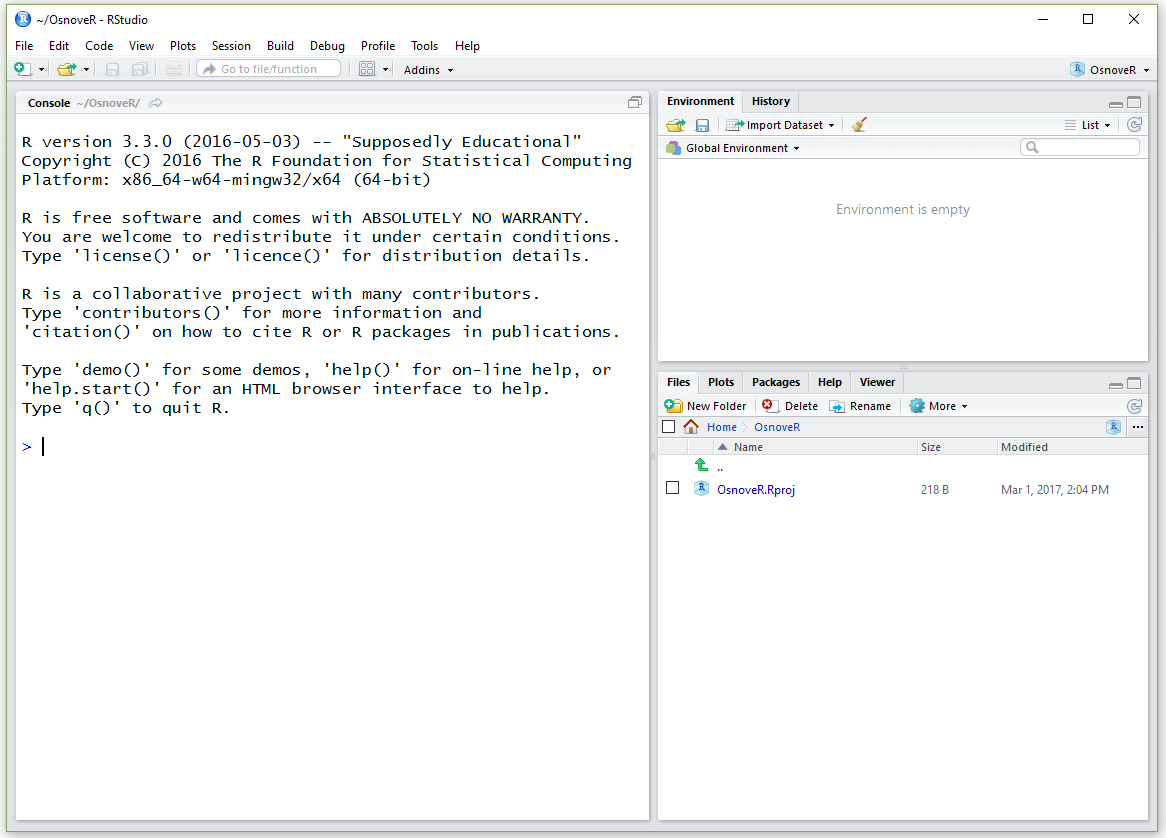
\includegraphics{figures/RStudio1.png}
\caption{\label{fig:unnamed-chunk-3}Izgled sucelja RStudio}
\end{figure}

Ukoliko je došlo do nekih problema, provjerite da li ste ispravno
proveli sve navedene korake instalacije. U nastavku ćemo se pozabaviti
detaljima prikazanog sučelja.

\begin{center}\rule{0.5\linewidth}{\linethickness}\end{center}

\section{\texorpdfstring{Pregled razvojnog sučelja
\emph{RStudio}}{Pregled razvojnog sučelja RStudio}}\label{pregled-razvojnog-sucelja-rstudio}

Pogledajmo sučelje \emph{RStudio}. Vidimo da je podijeljeno na tri
prozora - lijevi dio je ``radni'' i u njega upisujemo programski kod. S
desne strane se nalaze pomoćni prozori koji prikazuju različite stvari,
ovisno o odabranoj kartici; u gornjem desnom dijelu između ostalog
možemo vidjeti što se trenutno nalazi u našoj radnoj okolini (koja je na
početku prazna) te povijest naredbi koje smo izvršavali. Donji dio služi
za prikaz dokumentacije, datoteka u radnoj mapi, instaliranih paketa,
vizualizacija i sl.

\begin{center}\rule{0.5\linewidth}{\linethickness}\end{center}

\subsection{Interaktivna konzola}\label{interaktivna-konzola}

Vratimo se na lijevi dio sučelja. Ovdje se zapravo radi o tzv.
``interaktivnoj konzoli''. Naime, po svojoj prirodi R je tzv.
``interpreterski jezik'' u smislu da se naredbe odmah interpretiraju i
izvršavaju. Iako je moguće izrađivati i veće skripte koje se onda
izvršavaju ``u komadu'', rad sa jezikom R vrlo često se svodi na princip
\emph{naredba - odgovor}. Upravo zbog toga govorimo o ``interaktivnoj
programskoj analizi podataka'' - analitičar ``programira'' upisivanjem
naredbi te u svakom trenutku može proučiti dobivene međurezultate i
odlučiti se na daljnje korake.

\begin{center}\rule{0.5\linewidth}{\linethickness}\end{center}

Prikažimo kako radi interaktivna konzola. Uz pomoć tipkovnice možemo
utipkati jednostavan matematički izraz - npr. \texttt{3\ +\ 2} i
stisnuti tipku \emph{ENTER}. Vidimo da će nam R odmah pružiti rezultat -
možemo ga koristiti i kao kalkulator!

Za matematičke izraze koje nije jednostavno ``utipkati'' moramo
koristiti funkcije. Tako npr. drugi korijen možemo izračunati uz pomoć
funkcije \texttt{sqrt()}. Pokušajmo u konzolu utipkati \texttt{sqrt(10)}
i stisnuti \emph{ENTER}. R nam opet odmah prikazuje rezultat. U ovom
trenutku zaslon bi nam trebao izgledati otprilike kao na sljedećoj
slici.

\begin{figure}
\centering
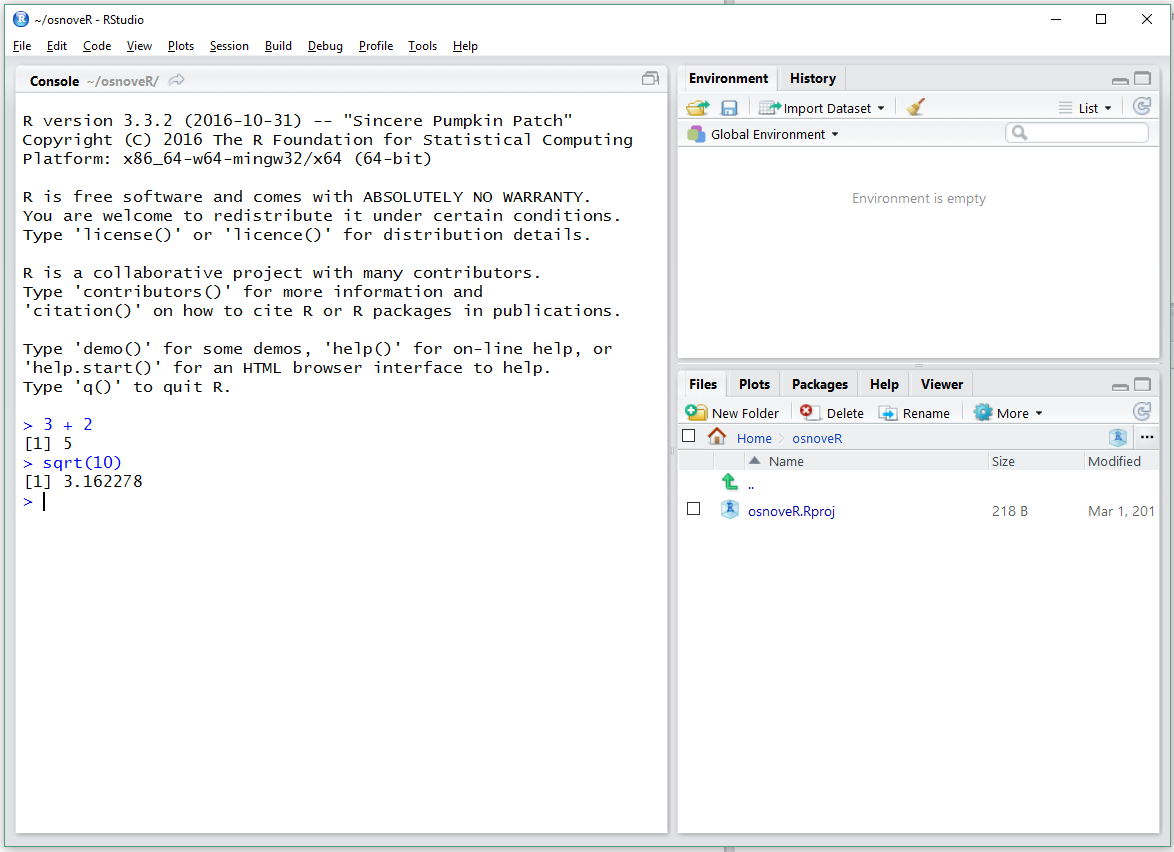
\includegraphics{figures/RStudio2.png}
\caption{\label{fig:unnamed-chunk-4}R kao kalkulator}
\end{figure}

Jedan od problema ovakvog načina korištenja R-a jest taj što nam se
miješaju naredbe i rezultati, a povijest niza naredbi postaje sve teže
vidljiva kako se korištenjem konzole spuštamo sve ``niže i niže''. Isto
tako, ako iz nekog razloga naredba koju izvršavamo rezultira greškom
koju pokušavamo ispraviti, konzola vrlo brzo postaje ``prljava'' budući
da se miješaju korektni pozivi sa izvještajima o greškama čime bilo
kakva složenija procedura koju želimo provesti postaje ``rastrgana'' i
nepregledna. Zbog toga analitičari vrlo često koriste tzv. ``R skripte''
koje omogućuju da vizualno izdvojimo naredbe koje želimo izvršiti od
same konzole, ali i dalje uz mogućnost da ih lako upišemo u konzolu,
slijedno izvršimo i pogledamo rezultat.

\begin{center}\rule{0.5\linewidth}{\linethickness}\end{center}

\subsection{Pisanje R skripti}\label{pisanje-r-skripti}

Na alatnoj traci odaberimo
\texttt{File\ -\textgreater{}\ New\ File\ -\textgreater{}\ R\ Script}
(ili stisnemo kombinaciju tipaka CTRL + SHIFT + N).

Vidimo da se ``radni dio'' na lijevoj strani razdvojio na dva dijela.
Gornji dio predstavlja prostor za našu ``skriptu'' - zapravo niz naredbi
koje želimo izvršiti - dok interaktivna konzola sada zauzima donji dio
radne plohe. Ukoliko želimo, možemo pomicanjem granice promijeniti
veličinu ovih (a i ostalih prozora), no za sada je bitno da imamo
pregled i skripte i konzole.

Upišimo dvije naredbe u prozor za pisanje skripte - prva neka bude
\texttt{print("Pozdrav!")} a ispod nje opet jednostavan matematički
izraz \texttt{3\ +\ 4}. Vratimo kursor na prvi redak i stisnimo
kombinaciju tipki CTRL + ENTER. Ukoliko smo ispravno pratili navedene
korake, naredba na mjestu koje se nalazio kursor automatski će se
preslikati u interaktivnu konzolu i izvršiti. Kursor će sada biti na
mjestu sljedeće naredbe koju također možemo izvršiti sa CTRL + ENTER.
Zaslon bi sada trebao izgledati slično sljedećoj slici.

\begin{figure}
\centering
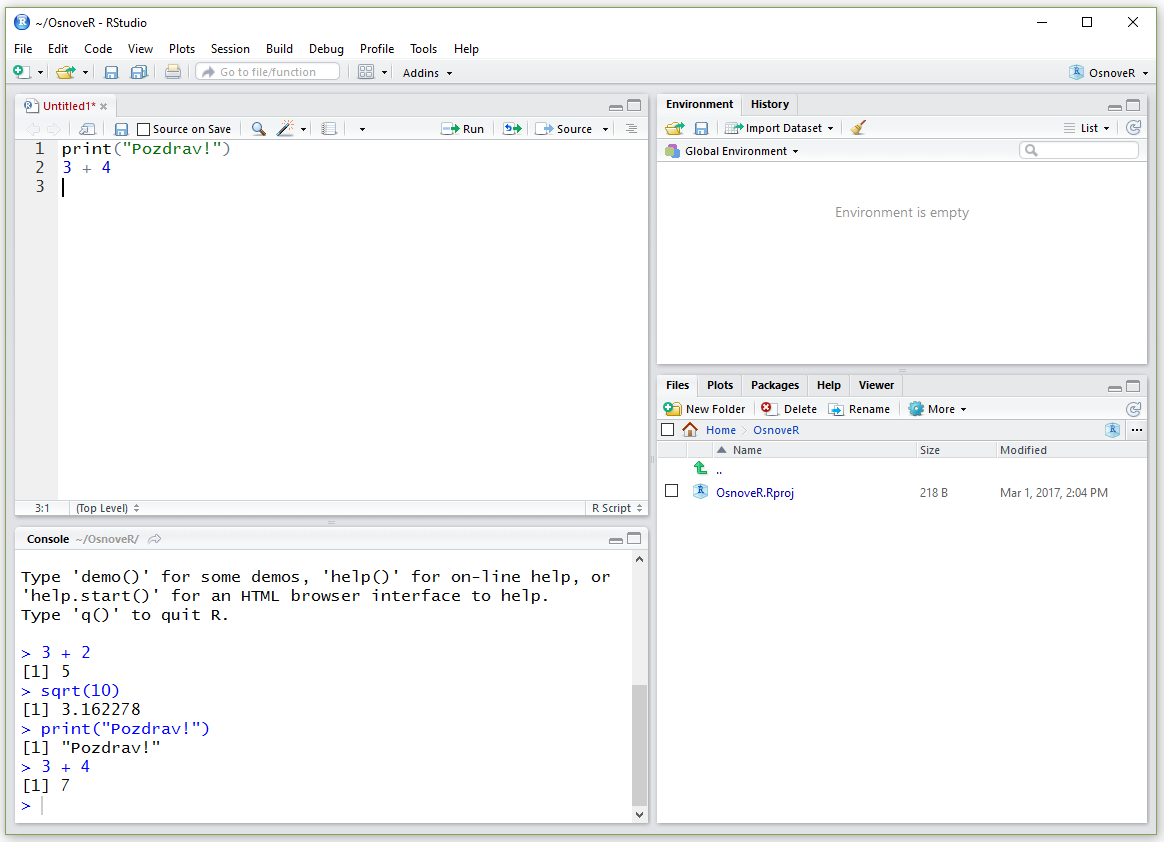
\includegraphics{figures/RStudio3.png}
\caption{\label{fig:unnamed-chunk-5}R skripta}
\end{figure}

Ovo je zapravo uobičajeni način rada u jeziku R - u prostor za skripte
upisujemo naredbe koje potom izvršavamo njihovim automatskim
preslikavanjem u konzolu. Ako nešto ne štima s naredbom, lako ju
preinačimo i ponovo izvršimo. Ukoliko želimo izvesti blok naredbi,
odaberemo ih povlačenjem miša i izvršimo kombinacijom tipaka CTRL +
ENTER. Skripte možemo proširiti komentarima (koji počinju znakom
\texttt{\#} kojeg R interpretira kao ``ovaj redak ignoriraj''), a na
kraju rada spremiti pod odabranim imenom na čvrsti disk.

No možemo otići i korak dalje. Iako su R skripte sasvim adekvatne za
ugodan rad u jeziku R, postoji dodatna tehnologija koja nam omogućuje
još veću fleksibilnost u radu sa programskim jezikom R - \emph{R
Markdown}.

\begin{center}\rule{0.5\linewidth}{\linethickness}\end{center}

\subsection{\texorpdfstring{\emph{R
Markdown}}{R Markdown}}\label{r-markdown}

Pisanje R skripti vrlo je slično klasičnom poimanju ``programiranja'' -
pišemo programske naredbe koje se u pravilu izvršavaju slijedno te
kojima opcionalno dodajemo komentare u svrhu dokumentacije. No budući da
je rad u R-u vrlo često interaktivne prirode te da se kao završni korak
neke analize podataka obično očekuje oblikovanje izvještaja koji će na
adekvatan način prikazati dobivene rezultate, sučelje RStudio podržava
tehnologiju koja omogućuje učinkovitu kombinacije programiranja i
strukturiranog dokumentiranja na principu ``interaktivne bilježnice''``;
analitičar može pisati''čisti" tekst, opcionalno sa formulama, slikama
te izmjenama veličine i prirode tekstualnog fonta, da bi potom u takav
tekst ``ugradio'' izvršivi programski kod zajedno sa njegovim
rezultatima. Tehnologija koja ovo omogućuje je tzv. \textbf{R Markdown},
koji je relativno nedavno proširen novim konceptom nazvanim \textbf{R
Notebook}.

Rad ove tehnologije najlakše je prikazati preko primjera - u alatnoj
traci odaberimo
\texttt{File\ -\textgreater{}\ New\ File\ -\textgreater{}\ R\ Markdown...}
te u idućem prozoru odaberimo proizvoljni naslov (npr. \texttt{Proba}),
opcionalno ime autora te jednu od opcija za konačni oblik izvještaja
(preporučeno HTML zbog najmanje ovisnosti o dodatnim paketima).

\begin{center}\rule{0.5\linewidth}{\linethickness}\end{center}

Za razliku od R skripte, R će kod novog \emph{R Markdown} dokumenta
stvoriti ``popunjeni'' dokument. Ovo je izvedeno na ovaj način iz
jednostavnog razloga da korisnik dobije predložak koji istovremeno služi
i kao podsjetnik te kojeg onda lako izmjeni prema svojem nahođenju. Mi
ćemo za naše potrebe obrisati veći dio ovog predloška - sve poslije
inicijalnog zaglavlja, tj. ispod druge pojave znakova \texttt{-\/-\/-}.

Potom možemo ispod napisati bilo kakav tekst. Znakovima \texttt{\#},
\texttt{\#\#}, \texttt{\#\#\#} itd. možemo postaviti naslov određene
kategorije (to sada nisu komentari, jer ovo zapravo nije R kod!), dok
znakovima \texttt{*} i \texttt{**} ispred i iza odabranih riječi
odabiremo nakošeni ili masni otisak u konačnom izvještaju. Ovo je tzv.
čisti ``\emph{markdown}'', tj. običan tekst koji se uz pomoć dodatnih
alata može pretvoriti u oblikovani tekst, ukoliko želimo.

Kada želimo u ovaj naš ``izvještaj'' ugraditi programski kod, moramo
stvoriti tzv. ``isječak'' (engl. \emph{chunk}). To možemo učiniti
odabirom \texttt{Insert\ -\textgreater{}\ R} na alatnoj traci ili
kombinacijom tipaka CTRL + ALT + I.

Uočite da isječak počinje i završava posebno odabranim nizom znakova -
tri ``apostrofa nalijevo'' (engl. \emph{backticks}). Isto tako, početak
isječka u vitičastim zagradama opisuje parametre isječka, od čega je
najvažniji programski jezik kojeg ćemo koristiti. U ovom udžbeniku ćemo
gotovo isključivo koristiti jezik R, iako je moguće koristiti i druge
jezike ukoliko su oni instalirani na platformi na kojoj je pokrenut
\emph{RStudio}.

Isječak koda ponaša se isto kao i standardna R skripta - možemo
upisivati naredbe i izvršavati ih. Razlika je samo u tome što - ukoliko
želimo - rezultate možemo vidjeti i odmah u samom \emph{R Markdown}
dokumentu. Ako nam ova opcija smeta možemo ju isključiti (klik na
zupčanik u alatnoj traci i odabir \texttt{Chunk\ output\ in\ console})
no u pravilu nam odgovara da se rezultat ugradi u dokument kako bi
naknadno mogli ponovo pregledavati rezultate prethodnih isječaka.

Ako smo pratili upute, zaslon bi mogao izgledati slično sljedećoj slici:

\begin{figure}
\centering
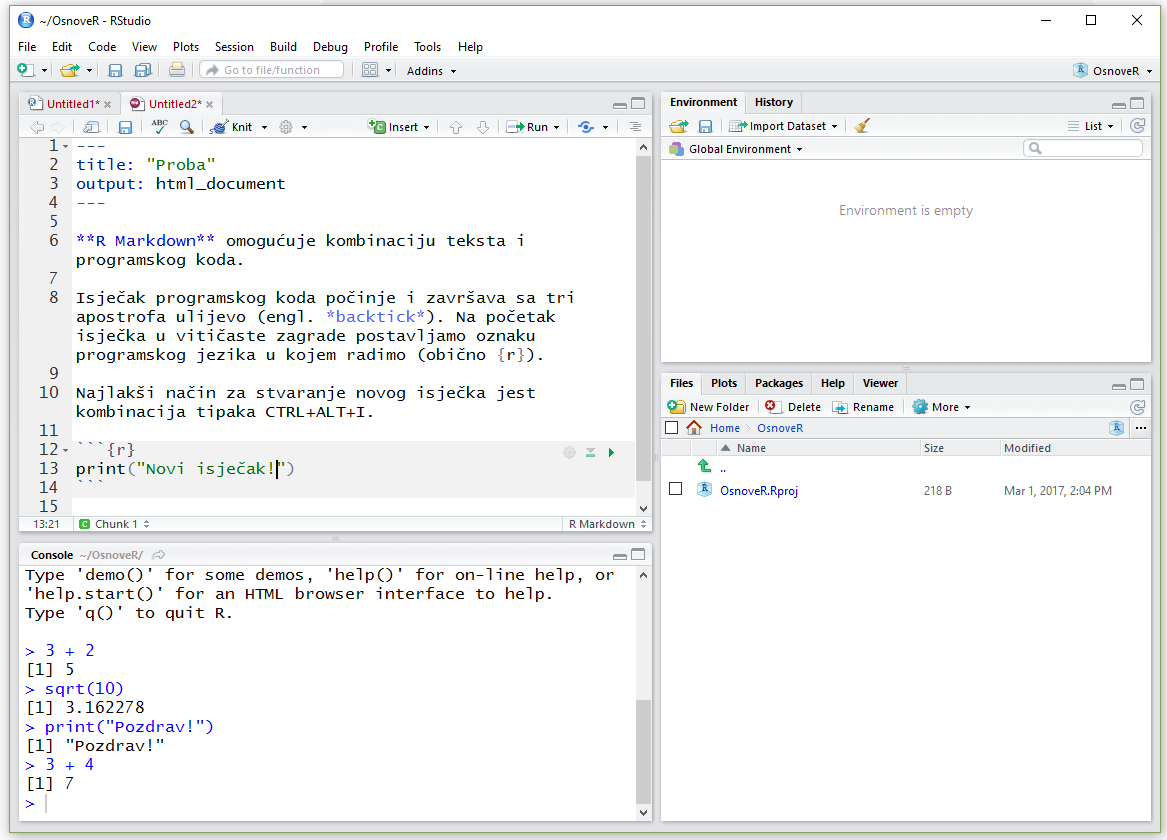
\includegraphics{figures/RStudio4.png}
\caption{\label{fig:unnamed-chunk-6}R Markdown dokument}
\end{figure}

Ukoliko želimo, možemo pokušati stvoriti ``izvještaj'' od trenutnog
dokumenta. Prvo ga moramo spremiti pod određenim imenom (npr.
\texttt{Proba.rmd}), a potom možemo kliknuti na gumb \texttt{Knit} koji
će dokument iz čistog teksta pretvoriti u HTML datoteku.

\emph{R Markdown} dokumenti su puno moćniji nego što se možda daje
naslutiti do sada prikazanim elementima. Isječcima možemo dodavati niz
parametara kako bismo utjecali na njihovo ponašanje. Izlazni oblik može
biti PDF, DOCX ali i drugi oblici kao što slajdovi raznih tehnologija,
knjige namijenjene mobilnim uređajima, interaktivna Web aplikacija i sl.
Udžbenik kojeg čitate zapravo nije ništa drugo do niz RMD datoteka
pretvoren u adekvatni oblik kojeg trenutno koristite. Kao što ćemo
objasniti u sljedećem poglavlju, RMD datoteke su također i glavni način
na kojeg ćete moći na interaktivan način pratiti ovaj udžbenik i
isprobavati primjere i zadatke koje slijede. Univerzalnost i
fleksibilnost tehnologije \emph{R Markdown} je iznimno velika, čemu u
prilog govori i njezina velika popularnost u R zajednici.

\begin{center}\rule{0.5\linewidth}{\linethickness}\end{center}

\section{Kako koristiti ovaj
udžbenik?}\label{kako-koristiti-ovaj-udzbenik}

Osnovna ideja ovog udžbenika jest ``učenje kroz primjenu''. Zbog toga se
u lekcijama u nastavku neće koristiti previše primjera, već se čitatelja
potiče da svaki novi koncept usvoji kroz rješavanje niza lakših i težih
zadataka.

Svako poglavlje koje slijedi ima prateću ``radnu bilježnicu''.
Jednostavno rečeno, radi se o RMD datoteci koja sadrži sve primjere iz
zadatke iz ovog udžbenika, popraćene sažetim tekstom radi lakšeg
snalaženja i referenciranja na koncepte koji se obrađuju. Osnovna ideja
je da čitatelj paralelno čita udžbenik i rješava radnu bilježnicu,
gledajući rješenje zadatka tek nakon što ga samostalno riješi unutar
programskog alata.

Poneki zadaci zahtijevati će jednostavno uklanjanje znaka \texttt{\#}
(koji označava ``komentar'') sa početka naredbe te njezino izvršavanje.
Usprkos trivijalnom pristupu, na ovaj način se ipak jasnije potiče
čitatelja za samostalno isprobavanje naredbe, umjesto da samo pogleda
njezin rezultat. Drugi zadaci zahtijevati će nešto veći angažman.
Konačno, nakon svake lekcije nalazi se niz ``Zadataka za vježbu'' uz
koje se neće nalaziti rješenje te koji će predstavljati svojevrsnu
provjeru svih danih koncepata lekcije. Čitateljima se snažno preporučuje
rješavanje svih primjera i zadataka prije prelaska na iduću lekciju,
budući da lekcije koje slijede pretpostavljaju dobro usvojeno znanje
svih do tada obrađenih tema.

Naravno, udžbenik je moguće čitati i bez navedenog ``interaktivnog''
pristupa. Rješenja uz zadatke otkrivaju ispravnu metodu pristupa
problemu, a većina naredbi popraćena je ispisom kojeg bi korisnik dobio
na zaslonu njihovim izvršavanjem. Usprkos tome, stav autora udžbenika
jest da se programski jezici ne mogu učiti čitanjem te da se dodatni
trud isprobavanja svih, pa čak i najjednostavnijih koncepata, u
konačnici višestruko isplati.

\begin{center}\rule{0.5\linewidth}{\linethickness}\end{center}

Upoznajmo se pobliže sa konceptom radnih bilježnica. Prvo je potrebno
pronaći i otvoriti radnu bilježnicu koja odgovara lekciji koju čitate.
Nju je lako prepoznati prema odgovarajućem broju lekcije - radna
bilježnica za ovu lekciju nosi naziv \texttt{01\_Uvod\_RB.Rmd}.
Preporučuje se da sve radne bilježnice na kojima namjeravati raditi
kopirate negdje na lokalno računalo zajedno sa svim pratećim datotekama
koje se nalaze u istoj mapi ako ih ima.

Kao što je rečeno, radna bilježnica će u pravilu sadržavati sav
programski kod lekcije na koje se odnosi, ali samo dio teksta koliko je
dovoljno za lakše snalaženje. Ukoliko ovaj tekst čitate direktno iz
radne bilježnice, a ne kao dio udžbenika, možete vidjeti da nedostaje
cijeli prethodni dio lekcije; to je zato što se uvodni koraci opisani u
njemu tiču koncepata koje je potrebno usvojiti prije korištenja radne
bilježnice. Ako ih niste prošli, preporuka je da se vratite i prođete ih
te potom nastavite sa primjerima i zadacima koji slijede.

Radne bilježnice razlikuju \textbf{Primjere} i \textbf{Zadatke}.
Primjere je u pravilu potrebno samo izvršiti. Zadaci s druge strane
očekuju izvjesne preinake ili unos novog programskog koda. Kao što je
rečeno, udžbenik će postaviti daleko veći naglasak na zadatke.

Primjer može izgledati ovako:

\begin{center}\rule{0.5\linewidth}{\linethickness}\end{center}

\textbf{Primjer - nekoliko jednostavnih naredbi R programskog jezika}

\begin{Shaded}
\begin{Highlighting}[]
\DecValTok{3}\OperatorTok{+}\DecValTok{2}         \CommentTok{#zbrajanje}
\KeywordTok{log}\NormalTok{(}\DecValTok{10}\NormalTok{)    }\CommentTok{# prirodni logaritam!}
\KeywordTok{log10}\NormalTok{(}\DecValTok{10}\NormalTok{)   }\CommentTok{# ovo je logaritam baze 10! Usput, komentare pišemo znakom "#"}
\KeywordTok{sin}\NormalTok{(}\FloatTok{0.5} \OperatorTok{*}\StringTok{ }\NormalTok{pi)      }\CommentTok{# pi je jedna od ugrađenih konstanti}
\end{Highlighting}
\end{Shaded}

\begin{verbatim}
## [1] 5
## [1] 2.302585
## [1] 1
## [1] 1
\end{verbatim}

Naredbe iz primjera možete izvršiti pojedinačno, ili cijeli isječak
odjednom kombinacijom tipaka CTRL + SHIFT + ENTER. Nikakve preinake koda
nisu nužne (iako često nije loše eksperimentirati sa danim naredbama!).

Zadaci s druge strane uvijek traže određenu - makar minimalnu -
intervenciju.

\begin{center}\rule{0.5\linewidth}{\linethickness}\end{center}

\textbf{Zadatak 1.1 - naredbe za provjeru i izmjenu radne mape}

\begin{Shaded}
\begin{Highlighting}[]
\CommentTok{# izvršite sljedeće naredbe uklanjanjem znaka komentara}

\CommentTok{#getwd()     # mapa u kojoj trenutno radimo}
\CommentTok{#setwd(".")  # ovdje možemo navesti novu radnu mapu ukoliko želimo}
\end{Highlighting}
\end{Shaded}

\begin{Shaded}
\begin{Highlighting}[]
\KeywordTok{getwd}\NormalTok{()     }\CommentTok{# mapa u kojoj trenutno radimo}
\KeywordTok{setwd}\NormalTok{(}\StringTok{"."}\NormalTok{)  }\CommentTok{# ovdje možemo navesti novu radnu mapu ukoliko želimo}
\end{Highlighting}
\end{Shaded}

\begin{center}\rule{0.5\linewidth}{\linethickness}\end{center}

Zadatak će se često odnositi na upravo uvedeni koncept. Npr. zgodno je
za napomenuti da, iako jezik R podržava operator \texttt{=} za
pridruživanje vrijednosti nekoj varijabli, preporučuje se korištenje
operatora \texttt{\textless{}-} u tu svrhu koji je nešto više
``R-ovski''. Također, uočimo da R podržava tzv. \emph{autoprint}, tj.
uvijek će ispisati rezultat zadnje naredbe na zaslon. To znači da ako u
isječku stvaramo novu varijablu \texttt{x} te ju želimo ispisati na
zaslon, ne moramo kao zadnju naredbu staviti \texttt{print(x)} već je
dovoljno staviti samo \texttt{x}. Isprobajmo ovo u zadatku.

\begin{center}\rule{0.5\linewidth}{\linethickness}\end{center}

\textbf{Zadatak 1.2 - R-ovski operator pridruživanja}

\begin{Shaded}
\begin{Highlighting}[]
\CommentTok{# upišite `5` u varijablu `x`}
\CommentTok{# potom ispišite varijablu `x` na zaslon}
\end{Highlighting}
\end{Shaded}

\begin{Shaded}
\begin{Highlighting}[]
\NormalTok{x <-}\StringTok{ }\DecValTok{5}
\NormalTok{x}
\end{Highlighting}
\end{Shaded}

\begin{verbatim}
## [1] 5
\end{verbatim}

\begin{center}\rule{0.5\linewidth}{\linethickness}\end{center}

Sada kada smo se dobro upoznali sa radnom platformom, možemo početi sa
učenjem osnovnih elemenata programskog jezika R.

\begin{center}\rule{0.5\linewidth}{\linethickness}\end{center}

{Programirajmo u R-u} by Damir Pintar is licensed under a Creative
Commons Attribution-NonCommercial-NoDerivatives 4.0 International
License.Based on a work at https://ratnip.github.io/FER\_OPJR/

\chapter{Osnovni tipovi podataka i operatori}\label{tipovi}

\begin{center}\rule{0.5\linewidth}{\linethickness}\end{center}

``Osnovni'' ili ``primitivni'' tipovi podataka su temeljni izgradbeni
blokovi programskih jezika. Ovdje se najčešće misli na ugrađene
mehanizme koji omogućuju pohrane elementarne informacije - najčešće
logičkog, numeričkog ili znakovnog tipa. Većina programskih jezika
koristi iste ili vrlo slične načine pohrane takvih informacija, što
znači da implementira slične osnovne tipove podataka - razlika je često
u detaljima kao što su odabrani nazivu tipa, nazivni broj bajtova i sl.
U svakom slučaju najčešći prvi korak kod učenja novog programskog jezika
jest upoznavanje osnovnih tipova podataka koje isti podržava.

Sljedeća stvar koja nas potom može zanimati jest sintaksa jezika, tj.
način na kojeg pišemo naredbe koje interpreter jezika može razumjeti i
izvršiti. Jezik R u svojoj sintaksi slijedi slične konvencije viđene u
jezicima kao što su \emph{Python}, \emph{Ruby} ili \emph{Java}, naravno
uz određene specifičnosti (kao i svaki pojedini programski jezik). Neka
osnovna sintaksna pravila su: svaka naredba u pravilu mora ići u svoj
redak, ali uvlačenje naredbi nije bitno kao ni stavljanje točke-zareza
na kraj naredbe; blokove definiramo vitičastim zagradama; tipove
varijabli ne moramo definirati unaprijed već se oni samo prilagođavaju
pridruženoj vrijednosti; komentari započinju znakom \texttt{\#}; i sl.
Sintaksu ćemo najbolje naučiti kroz primjere - učenjem elemenata jezika
sintaksna pravila često postaju intuitivno jasna. Najbolje je krenuti sa
jednostavnim funkcijama i operatorima, što ćemo i učiniti u ovoj
lekciji.

Lekciju ćemo završiti raspravom o tzv. ``nedostajućim'' ili
``nepostojećim'' vrijednostima. Budući da R ima svoj vlastiti način
definiranja takve vrste vrijednosti, odmah ćemo pojasniti način na koji
su one u R-u implementirane kako bi u lekcijama koje slijede bili
pripremljeni za lako upravljanje takvim vrijednostima (koje se vrlo
često susreću u radu sa stvarnim podatkovnim skupovima).

\begin{center}\rule{0.5\linewidth}{\linethickness}\end{center}

\section{Osnovni tipovi podataka}\label{osnovni-tipovi-podataka}

R poznaje šest osnovnih tipova podataka:

\begin{longtable}[]{@{}lll@{}}
\toprule
tip & izvorni naziv tipa & primjeri\tabularnewline
\midrule
\endhead
logički & \emph{logical} & \texttt{TRUE}, \texttt{FALSE} ili \texttt{T},
\texttt{F}\tabularnewline
cjelobrojni & \emph{integer} & \texttt{2L}, \texttt{5L},
\texttt{123456789L}\tabularnewline
realni & \emph{double} & \texttt{4}, \texttt{6}, \texttt{3.14},
\texttt{2e5}\tabularnewline
kompleksni & \emph{complex} & \texttt{5\ +\ 2i},
\texttt{7\ +\ 1i}\tabularnewline
znakovni & \emph{character} & \texttt{"A"}, \texttt{"B"},
\texttt{"Pero"}, \texttt{"ABCDEFGHijklmnoPQRSTUVwyz"}\tabularnewline
bajtovi & \emph{raw} & \texttt{as.raw(2)},
\texttt{charToRaw("1")}\tabularnewline
\bottomrule
\end{longtable}

Neke opaske:

\begin{itemize}
\tightlist
\item
  cjelobrojni i realni tipovi se često zajedno tretiraju kao tip
  \texttt{numeric} (iako ovo nije u potpunosti konzistentno!)
\item
  kompleksni tip mora imati deklariranu imaginarnu konstantu čak i ako
  je ona 1 (\texttt{2\ +\ i} nije dobar zapis!)
\item
  tip ``sirovih'' bajtova se relativno rijetko koristi
\end{itemize}

Provjeru da li je neka varijabla određenog tipa možemo raditi uz pomoć
funkcije \texttt{is.\textless{}naziv\_tipa\textgreater{}}. Ovo ćemo
isprobati u sljedećem zadatku. Prije nego što počnemo s rješavanjem
uvedimo jedan novitet: u zadacima gdje ispisujemo više stvari na zaslon
korisno je vizualno odvojiti različite segmente ispisa kako bismo lakše
shvatili na koji dio koda se referenciraju. U tu svrhu ćemo koristiti
naredbu \texttt{cat("-\/-\/-\/-\/-\/-\/-\/-\/-\/-\/-\textbackslash{}n")}
koja jednostavno na zaslon ispisuje niz crtica i prelazi u novi red.
Mogli smo koristiti i funkciju \texttt{print()}, no ona uvijek započinje
ispis sa indeksom elementa dok naredba \texttt{cat} predstavlja
``sirovi'' ispis, što nam u ovom slučaju više odgovara.

\begin{center}\rule{0.5\linewidth}{\linethickness}\end{center}

\textbf{Zadatak 2.1 - provjera tipova podataka}

\begin{Shaded}
\begin{Highlighting}[]
\CommentTok{#isprobajte sljedeće naredbe:}
\CommentTok{#is.logical(FALSE)}
\CommentTok{#is.integer(2L)}
\CommentTok{#is.double(1.11)}

\CommentTok{# izvedite sljedeće provjere:}

\CommentTok{# da li je 5L numerički tip?}
\CommentTok{# da li je 3.14 numerički tip?}
\CommentTok{# da li je "ABC" znakovni tip?}
\CommentTok{# da li je 4 + 2i kompleksni tip?}
\CommentTok{# da li je 5 cjelobrojni tip?}
\end{Highlighting}
\end{Shaded}

\begin{Shaded}
\begin{Highlighting}[]
\KeywordTok{is.logical}\NormalTok{(}\OtherTok{FALSE}\NormalTok{)}
\KeywordTok{is.integer}\NormalTok{(2L)}
\KeywordTok{is.double}\NormalTok{(}\FloatTok{1.11}\NormalTok{)}

\KeywordTok{cat}\NormalTok{(}\StringTok{"-----------}\CharTok{\textbackslash{}n}\StringTok{"}\NormalTok{)}

\KeywordTok{is.numeric}\NormalTok{(5L)}
\KeywordTok{is.numeric}\NormalTok{(}\FloatTok{3.14}\NormalTok{)}
\KeywordTok{is.character}\NormalTok{(}\StringTok{"ABC"}\NormalTok{)}
\KeywordTok{is.complex}\NormalTok{(}\DecValTok{4} \OperatorTok{+}\StringTok{ }\NormalTok{2i)}
\KeywordTok{is.integer}\NormalTok{(}\DecValTok{5}\NormalTok{)}
\end{Highlighting}
\end{Shaded}

\begin{verbatim}
## [1] TRUE
## [1] TRUE
## [1] TRUE
## -----------
## [1] TRUE
## [1] TRUE
## [1] TRUE
## [1] TRUE
## [1] FALSE
\end{verbatim}

\begin{center}\rule{0.5\linewidth}{\linethickness}\end{center}

Da li ste uočili nešto neobično u ovim provjerama? Pokušajte objasniti
dobiveni rezultat.

Tip neke varijable ili konstante možemo dohvatiti uz pomoć funkcija
\texttt{typeof} ili \texttt{class}. Razlika između njih je sljedeća:

\begin{itemize}
\tightlist
\item
  \texttt{typeof} - dohvaća ``primitivni'' ili ``osnovni'' tip podatka
  (\texttt{integer}, \texttt{double} )
\item
  \texttt{class} - ``objektni tip'', zapravo vrijednost atributa
  \texttt{class}
\end{itemize}

\begin{center}\rule{0.5\linewidth}{\linethickness}\end{center}

\textbf{Zadatak 2.2 - dohvat tipova podataka}

\begin{Shaded}
\begin{Highlighting}[]
\CommentTok{# ispišite tipove sljedećih konstanti: TRUE, 2L, F, 3.14, "ABC"}

\CommentTok{# ispišite klase istih konstanti. Ima li razlike?}
\end{Highlighting}
\end{Shaded}

\begin{Shaded}
\begin{Highlighting}[]
\KeywordTok{typeof}\NormalTok{(}\OtherTok{TRUE}\NormalTok{)}
\KeywordTok{typeof}\NormalTok{(2L)}
\KeywordTok{typeof}\NormalTok{(F)}
\KeywordTok{typeof}\NormalTok{(}\FloatTok{3.14}\NormalTok{)}
\KeywordTok{typeof}\NormalTok{(}\StringTok{"ABC"}\NormalTok{)}

\KeywordTok{cat}\NormalTok{(}\StringTok{"-----------}\CharTok{\textbackslash{}n}\StringTok{"}\NormalTok{)}

\KeywordTok{class}\NormalTok{(}\OtherTok{TRUE}\NormalTok{)}
\KeywordTok{class}\NormalTok{(2L)}
\KeywordTok{class}\NormalTok{(F)}
\KeywordTok{class}\NormalTok{(}\FloatTok{3.14}\NormalTok{)}
\KeywordTok{class}\NormalTok{(}\StringTok{"ABC"}\NormalTok{)}
\end{Highlighting}
\end{Shaded}

\begin{verbatim}
## [1] "logical"
## [1] "integer"
## [1] "logical"
## [1] "double"
## [1] "character"
## -----------
## [1] "logical"
## [1] "integer"
## [1] "logical"
## [1] "numeric"
## [1] "character"
\end{verbatim}

\begin{center}\rule{0.5\linewidth}{\linethickness}\end{center}

Podatke možemo eksplicitno pretvarati iz jednog tipa u drugi uz pomoć
funkcije \texttt{as.\textless{}naziv\_tipa\textgreater{}}:

\begin{center}\rule{0.5\linewidth}{\linethickness}\end{center}

\textbf{Zadatak 2.3 - pretvorba tipova podataka}

\begin{Shaded}
\begin{Highlighting}[]
\CommentTok{# Izvedite sljedeće pretvorbe i ispišite rezultat}

\CommentTok{#  2.35 u integer}
\CommentTok{#  TRUE u numeric}
\CommentTok{#  100L u character}
\CommentTok{#  2.35 u character}
\CommentTok{#  2e2  u character}
\CommentTok{#  0 u logical}
\CommentTok{#  2.75  u logical}
\end{Highlighting}
\end{Shaded}

\begin{Shaded}
\begin{Highlighting}[]
\KeywordTok{as.integer}\NormalTok{(}\FloatTok{2.35}\NormalTok{)}
\KeywordTok{as.numeric}\NormalTok{(}\OtherTok{TRUE}\NormalTok{)}
\KeywordTok{as.character}\NormalTok{(100L)}
\KeywordTok{as.character}\NormalTok{(}\FloatTok{2.35}\NormalTok{)}
\KeywordTok{as.character}\NormalTok{(}\FloatTok{2e2}\NormalTok{)}
\KeywordTok{as.logical}\NormalTok{(}\DecValTok{0}\NormalTok{)}
\KeywordTok{as.logical}\NormalTok{(}\FloatTok{2.75}\NormalTok{)}
\end{Highlighting}
\end{Shaded}

\begin{verbatim}
## [1] 2
## [1] 1
## [1] "100"
## [1] "2.35"
## [1] "200"
## [1] FALSE
## [1] TRUE
\end{verbatim}

\begin{center}\rule{0.5\linewidth}{\linethickness}\end{center}

\emph{R} će sam provoditi implicitnu pretvorbu ukoliko je moguća:

\begin{center}\rule{0.5\linewidth}{\linethickness}\end{center}

\textbf{Zadatak 2.4 - implicitna pretvorba}

\begin{Shaded}
\begin{Highlighting}[]
\CommentTok{# napišite izraze koji odgovaraju sljedećem i ispišite rezultat:}

\CommentTok{# aritmetički operator između logičke i numeričke varijable}
\CommentTok{# aritmetički operator između cjelobrojne i numeričke varijable}
\CommentTok{# logički operator negacije primjenjen na numeričku varijablu}
\end{Highlighting}
\end{Shaded}

\begin{Shaded}
\begin{Highlighting}[]
\CommentTok{# aritmetički operator između logičke i numeričke varijable}
\OtherTok{TRUE} \OperatorTok{+}\StringTok{ }\DecValTok{5}

\CommentTok{# aritmetički operator između cjelobrojne i numeričke varijable}
\NormalTok{5L  }\OperatorTok{+}\StringTok{ }\FloatTok{3.14}

\CommentTok{# logički operator negacije primjenjen na numeričku varijablu}
\OperatorTok{!}\DecValTok{25}
\end{Highlighting}
\end{Shaded}

\begin{verbatim}
## [1] 6
## [1] 8.14
## [1] FALSE
\end{verbatim}

\begin{center}\rule{0.5\linewidth}{\linethickness}\end{center}

Implicitna pretvorba će se izvesti samo ako je smislen - npr.
aritmetički operator između znakovne i numeričke varijable rezultirati
će greškom.

\begin{center}\rule{0.5\linewidth}{\linethickness}\end{center}

\section{Operatori}\label{operatori}

Kao i u drugim programskim jezicima, R dozvoljava korištenje operatora u
izrazima. Neki od češće korištenih operatora su:

\begin{itemize}
\tightlist
\item
  \emph{aritmetički} \texttt{+}, \texttt{-}, \texttt{*}, \texttt{/},
  \texttt{**} (potencija), \texttt{\%\%} (modulo), \texttt{\%/\%}
  (cjelobrojno dijeljenje)
\item
  \emph{usporedni} \texttt{\textless{}}, \texttt{\textless{}=},
  \texttt{\textgreater{}}, \texttt{\textgreater{}=}, \texttt{==},
  \texttt{!=}
\item
  \emph{logički} \texttt{!} (negacija), \texttt{\&\&} (skalarni ``i''),
  \texttt{\textbar{}\textbar{}} (skalarni ``ili''), \texttt{\&}
  (vektorski ``i''), \texttt{\textbar{}} (vektorski ``ili'')
\item
  \emph{pridruživanje} \texttt{\textless{}-} ili \texttt{=}
\end{itemize}

\begin{center}\rule{0.5\linewidth}{\linethickness}\end{center}

\textbf{Zadatak 2.5 - operatori}

\begin{Shaded}
\begin{Highlighting}[]
\CommentTok{# isprobajte izraze `5 / 2` i `5 %/% 2`}

\CommentTok{# provjerite koliko iznosi "17 na kvadrat" i "ostatak dijeljenja 101 sa 12"}

\CommentTok{# provjerite što je rezultat sljedećih izraza: `17 > 13`, `!TRUE`,  `5 && 0`, `0. || 2`}
\end{Highlighting}
\end{Shaded}

\begin{Shaded}
\begin{Highlighting}[]
\CommentTok{# isprobajte izraze `5 / 2` i `5 %/% 2`}
\DecValTok{5} \OperatorTok{/}\StringTok{ }\DecValTok{2}
\DecValTok{5} \OperatorTok\StringTok{ }\DecValTok{2}

\KeywordTok{cat}\NormalTok{(}\StringTok{"-----------}\CharTok{\textbackslash{}n}\StringTok{"}\NormalTok{)}

\CommentTok{# provjerite koliko iznosi "17 na kvadrat" i "ostatak dijeljenja 101 sa 12"}
\DecValTok{17} \OperatorTok{^}\StringTok{ }\DecValTok{2}
\DecValTok{101} \OperatorTok\StringTok{ }\DecValTok{12}

\KeywordTok{cat}\NormalTok{(}\StringTok{"-----------}\CharTok{\textbackslash{}n}\StringTok{"}\NormalTok{)}

\CommentTok{# provjerite što je rezultat sljedećih izraza: `17 > 13`, `!TRUE`,  `5 && 0`, `0. || 2`, }
\DecValTok{17} \OperatorTok{>}\StringTok{ }\DecValTok{13}
\OperatorTok{!}\OtherTok{TRUE}
\DecValTok{5} \OperatorTok{&&}\StringTok{ }\DecValTok{0}
\DecValTok{0}\NormalTok{. }\OperatorTok{||}\StringTok{ }\DecValTok{2}
\end{Highlighting}
\end{Shaded}

\begin{verbatim}
## [1] 2.5
## [1] 2
## -----------
## [1] 289
## [1] 5
## -----------
## [1] TRUE
## [1] FALSE
## [1] FALSE
## [1] TRUE
\end{verbatim}

\begin{center}\rule{0.5\linewidth}{\linethickness}\end{center}

Logičke vrijednosti i usporedne operatore najčešće ćemo koristiti kod
tzv. ``uvjetnog izvođenja naredbi'', poznatog iz drugih programskih
jezika kao ``\emph{IF ELSE}'' naredba. U R-u njezina sintaksa izgleda
ovako:

\texttt{if\ (izraz)\ \{blok\}\ else\ \{blok\}}

Isprobajmo ovu naredbu na sljedećem zadatku:

\begin{center}\rule{0.5\linewidth}{\linethickness}\end{center}

\textbf{Zadatak 2.6 - uvjetno izvođenje naredbi}

\begin{Shaded}
\begin{Highlighting}[]
\CommentTok{# napišite naredbu koja izvodi sljedeće:}
\CommentTok{# "ako je 100 paran broj ispiši 'Uspjeh!'"}
\end{Highlighting}
\end{Shaded}

\begin{Shaded}
\begin{Highlighting}[]
\ControlFlowTok{if}\NormalTok{ (}\DecValTok{100} \OperatorTok\StringTok{ }\DecValTok{2} \OperatorTok{==}\StringTok{ }\DecValTok{0}\NormalTok{) }\KeywordTok{print}\NormalTok{(}\StringTok{"Uspjeh!"}\NormalTok{)}
\end{Highlighting}
\end{Shaded}

\begin{verbatim}
## [1] "Uspjeh!"
\end{verbatim}

\begin{center}\rule{0.5\linewidth}{\linethickness}\end{center}

Uočili smo gore da imamo dvije vrste logičkih operatora za ``i'' i
``ili''. Razliku ćemo objasniti kasnije, za sada je dovoljno reći da se
kod uvjetnog izvođenja naredbi ili programskih petlji gotovo isključivo
koristimo operatorima \texttt{\&\&} i \texttt{\textbar{}\textbar{}}
(``C++ - ovski''" operatori!).

Isto tako, već smo spomenuli da R nudi dva operatora pridruživanja,
\texttt{\textless{}-} i \texttt{=}. Pogledajmo ima li očitih razlika
između njih.

\begin{center}\rule{0.5\linewidth}{\linethickness}\end{center}

\textbf{Zadatak 2.7 - operatori pridruživanja}

\begin{Shaded}
\begin{Highlighting}[]
\CommentTok{# stvorite varijable x i y i objema dodijelite broj 5, jednoj sa operatorom <-, }
\CommentTok{# drugoj sa operatorom =}
\CommentTok{# ispišite varijable na zaslon}
\CommentTok{# uočavate li razliku između ova dva operatora?}
\end{Highlighting}
\end{Shaded}

\begin{Shaded}
\begin{Highlighting}[]
\NormalTok{x <-}\StringTok{ }\DecValTok{5}
\NormalTok{y =}\StringTok{ }\DecValTok{5}
\NormalTok{x}
\NormalTok{y}
\end{Highlighting}
\end{Shaded}

\begin{verbatim}
## [1] 5
## [1] 5
\end{verbatim}

\begin{center}\rule{0.5\linewidth}{\linethickness}\end{center}

Kao što smo se mogli posvjedočiti, nema uočljivih razlika između
operatora \texttt{\textless{}-} i \texttt{=}. Neke sitnije razlike
zapravo postoje, no one nemaju gotovo utjecaj na uobičajeno korištenje
ovog operatora u praksi. U literaturi se za pridruživanje vrijednosti
novim varijablama može vidjeti i jedna i druga inačica, no mi ćemo u
nastavku primarno i konzistentno koristiti \texttt{\textless{}-},
ponajviše zato kako bi programski kod bio vizualno distinktivniji od
drugih programskih jezika.

Kod pridruživanja pazimo da je s lijeve strane tzv. ``lijeva
vrijednost'' (engl. \emph{lvalue}). Ovo u programerskom smislu
interpretiramo kao ``nešto u što se može pohraniti izračunata
vrijednost''.

\begin{Shaded}
\begin{Highlighting}[]
\NormalTok{x }\OperatorTok{+}\StringTok{ }\DecValTok{1}\NormalTok{ <-}\StringTok{ }\DecValTok{2}          \CommentTok{# greška!!!]}
\end{Highlighting}
\end{Shaded}

U pravilu se u R-u kao \emph{lvalue} koristi varijabla, iako se tu
ponekad može pojaviti i poziv funkcije. Ovu možda inicijalno zbunjujuću
pojavu razjasniti ćemo kasnije.

\begin{center}\rule{0.5\linewidth}{\linethickness}\end{center}

Imenovanje varijabli uglavnom slijedi pravila iz drugih programskih
jezika - dozvoljena su slova, brojke, podcrta ali i točka . Prvi simbol
mora biti slovo ili točka.

\begin{Shaded}
\begin{Highlighting}[]
\NormalTok{.mojaVarijabla <-}\StringTok{ }\DecValTok{5}   \CommentTok{#OK}
\NormalTok{moja.Varijabla <-}\StringTok{ }\DecValTok{5}  \CommentTok{#OK}
\NormalTok{_mojaVarijabla <-}\StringTok{ }\DecValTok{5}  \CommentTok{# nije OK}
\NormalTok{123Varijabla <-}\StringTok{ }\DecValTok{5}  \CommentTok{# nije OK}
\end{Highlighting}
\end{Shaded}

U praksi za varijable složenih imena trebamo odabrati jednu od sljedećih
konvencija:

\begin{Shaded}
\begin{Highlighting}[]
\NormalTok{mojaVarijabla <-}\StringTok{ }\DecValTok{1}    \CommentTok{# tzv. camelcase}
\NormalTok{moja_varijabla <-}\StringTok{ }\DecValTok{2}   \CommentTok{#  podcrta ili}
\NormalTok{moja.varijabla <-}\StringTok{ }\DecValTok{3}   \CommentTok{# točka}
\end{Highlighting}
\end{Shaded}

Bitno je da u programskom kodu ne miješamo konvencije tj. da nakon
odabira budemo konzistentni.

Ukoliko baš inzistiramo na čudnim imenima koja koriste specijalne
znakove, onda ih moramo staviti pod tzv. ``lijeve jednostruke
apostrofe'' (engl. \emph{backticks}):

\begin{center}\rule{0.5\linewidth}{\linethickness}\end{center}

\textbf{Zadatak 2.8 - ime varijable sa specijalnim znakovima}

\begin{Shaded}
\begin{Highlighting}[]
\CommentTok{# upišite proizvoljno ime sa specijalnim znakovima unutar lijevih apostrofa }
\CommentTok{# i ispišite vrijednost varijable}
\CommentTok{#`` <- 2               }
\end{Highlighting}
\end{Shaded}

\begin{Shaded}
\begin{Highlighting}[]
\StringTok{`}\DataTypeTok{!%^$*@__=}\StringTok{`}\NormalTok{ <-}\StringTok{ }\DecValTok{2} 
\StringTok{`}\DataTypeTok{!%^$*@__=}\StringTok{`}
\end{Highlighting}
\end{Shaded}

\begin{verbatim}
## [1] 2
\end{verbatim}

Ovakav način imenovanja varijabli nije previše koristan u praksi, ali
ima i svoju svrhu - budući da su operatori u R-u zapravo funkcije (čija
su imena doslovno \texttt{+}, \texttt{**} i sl.) upotrebom lijevih
apostrofa možemo ih direktno referencirati u njihovom originalnom
obliku, što se može pokazati vrlo praktičnim kod tzv. funkcijskog
programiranja (o čemu ćemo govoriti u jednoj od budućih lekcija).

\begin{center}\rule{0.5\linewidth}{\linethickness}\end{center}

Pridjeljivanje vrijednosti novim nazivima varijabli mi zapravo stvaramo
nove varijable u radnoj okolini (koja se u R-u naziva ``globalna
okolina''). Sve varijable koje smo do sada stvorili možemo vidjeti uz
pomoć funkcije \texttt{ls()}. Ukoliko želimo obrisati neke varijable,
samo navedemo njihova imena u pozivu funkcije \texttt{rm()} (npr.
\texttt{rm(x,\ y,\ z)}). Za brisanje \emph{svih} varijabli iz radne
okoline koristimo poziv \texttt{rm(list=ls())}, s time što tu moramo
biti oprezni (nema ``\emph{undo}''!).

\begin{center}\rule{0.5\linewidth}{\linethickness}\end{center}

\textbf{Zadatak 2.9 - ispis i brisanje varijabli globalne okoline}

\begin{Shaded}
\begin{Highlighting}[]
\CommentTok{# ispišite sve do sada stvorene varijable globalne okoline}

\CommentTok{# obrišite neke od gore ispisanih varijabli - npr. rm(x, y, z)}
\CommentTok{# ponovo ispišite dostupne varijable}

\CommentTok{# obrišite SVE varijable globalne okoline}
\CommentTok{# (oprezno s ovim pozivom u praksi!)}
\CommentTok{# uvjerite se da je globalna okolina prazna}
\end{Highlighting}
\end{Shaded}

\begin{Shaded}
\begin{Highlighting}[]
\CommentTok{# ispišite sve do sada stvorene varijable globalne okoline}
\KeywordTok{ls}\NormalTok{()}

\CommentTok{# obrišite neke od upravo ispisanih varijabli - npr. rm(x, y, z)}
\CommentTok{# ponovo ispišite dostupne varijable}
\KeywordTok{rm}\NormalTok{(x, y)}
\KeywordTok{ls}\NormalTok{()}

\CommentTok{# obrišite SVE varijable globalne okoline}
\CommentTok{# (oprezno s ovim pozivom u praksi!)}
\CommentTok{# uvjerite se da je globalna okolina prazna}
\KeywordTok{rm}\NormalTok{(}\DataTypeTok{list=}\KeywordTok{ls}\NormalTok{())}
\KeywordTok{ls}\NormalTok{()}
\end{Highlighting}
\end{Shaded}

\begin{center}\rule{0.5\linewidth}{\linethickness}\end{center}

Konačno, kad god nam treba pomoć oko neke funkcije, imamo sljedeće
opcije na raspolaganju:

\begin{itemize}
\tightlist
\item
  napišemo samo \texttt{\textless{}ime\_funkcije\textgreater{}} (bez
  zagrada sa parametrima) i stisnemo \emph{} - ukoliko je funkcija
  pisana u \emph{R}-u (a nije samo \emph{proxy} prema implementaciji u
  C-u) na zaslon ćemo dobiti ispis izvornog koda funkcije
\item
  napišemo \texttt{help(\textless{}ime\_funkcije\textgreater{})} ili
  \texttt{?\textless{}ime\_funkcije\textgreater{}} čime dobijamo
  stranicu pomoći o funkciji sa popisom parametara, primjerima i sl.
\item
  napišemo \texttt{example(\textless{}ime\_funkcije\textgreater{})} pri
  čemu dobijemo popis primjera korištenja funkcije i dobivenih rezultata
\end{itemize}

Sljedeći isječak koda prikazuje način korištenja gornjih metoda (zbog
štednje prostora ne prikazujemo njihov rezultat).

\begin{Shaded}
\begin{Highlighting}[]
\CommentTok{#programski kod funkcije `ls`}
\NormalTok{ls}

\CommentTok{# pomoć za funkciju `ls`}
\NormalTok{?ls    }\CommentTok{# ili help(ls)}

\CommentTok{# primjeri korištenja funkcije `ls`}
\KeywordTok{example}\NormalTok{(ls)}
\end{Highlighting}
\end{Shaded}

\begin{center}\rule{0.5\linewidth}{\linethickness}\end{center}

\section{Nedostajuće, nepoznate i nemoguće
vrijednosti}\label{nedostajuce-nepoznate-i-nemoguce-vrijednosti}

U R-u postoji tri načina modeliranja ``nepostojećih'' vrijednosti:

\begin{itemize}
\tightlist
\item
  \texttt{NA} - (\emph{not available}) nedostajuća ili nepoznata
  vrijednost određenog tipa
\item
  \texttt{NaN} - (\emph{not a number}) ``nemogući'' broj, npr.
  \texttt{0/0}
\item
  \texttt{NULL} - nepostojeća vrijednost, doslovno ``ništa''
\end{itemize}

\begin{center}\rule{0.5\linewidth}{\linethickness}\end{center}

\textbf{Zadatak 2.10 - rad sa NA, NaN i NULL}

\begin{Shaded}
\begin{Highlighting}[]
\CommentTok{# Koliko je "5 + nepoznati broj"?}


\CommentTok{# Koliko je "5 + nepostojeći broj"?   }


\CommentTok{# provjerite klase sljedećih konstanti i izraza:}
   \CommentTok{#  NA}
   \CommentTok{#  aritmetička operacija između numeric i NA}
   \CommentTok{#  NaN}
   \CommentTok{#  NULL}
\end{Highlighting}
\end{Shaded}

\begin{Shaded}
\begin{Highlighting}[]
\CommentTok{# Koliko je "5 + nepoznati broj"?}
\DecValTok{5} \OperatorTok{+}\StringTok{ }\OtherTok{NaN}

\CommentTok{# Koliko je "5 + nepostojeći broj"?   }
\DecValTok{5} \OperatorTok{+}\StringTok{ }\OtherTok{NA}

\KeywordTok{cat}\NormalTok{(}\StringTok{"-----------}\CharTok{\textbackslash{}n}\StringTok{"}\NormalTok{)}

\CommentTok{# provjerite klase sljedećih konstanti i izraza i objasnite rezultat:}
   \CommentTok{#  NA}
   \CommentTok{#  aritmetička operacija između numeric i NA}
   \CommentTok{#  NaN}
   \CommentTok{#  NULL}
\KeywordTok{class}\NormalTok{(}\OtherTok{NA}\NormalTok{)        }\CommentTok{# logički tip je "najslabiji"!}
\KeywordTok{class}\NormalTok{(}\DecValTok{5} \OperatorTok{+}\StringTok{ }\OtherTok{NA}\NormalTok{)}
\KeywordTok{class}\NormalTok{(}\OtherTok{NaN}\NormalTok{)}
\KeywordTok{class}\NormalTok{(}\OtherTok{NULL}\NormalTok{)}
\end{Highlighting}
\end{Shaded}

\begin{verbatim}
## [1] NaN
## [1] NA
## -----------
## [1] "logical"
## [1] "numeric"
## [1] "numeric"
## [1] "NULL"
\end{verbatim}

\begin{center}\rule{0.5\linewidth}{\linethickness}\end{center}

Provjeru nedostajućih vrijednosti radimo slično provjeri tipova podataka
- koristimo funkcije \texttt{is.na}, \texttt{is.nan} i \texttt{is.null}.
Moramo voditi računa da je \texttt{NaN} zapravo podvrsta od \texttt{NA}
te da je \texttt{NULL} zapravo potpuno zasebna klasa sa specifičnim
ponašanjem - pokušaj aritmetičkih ili logičkih operacija nad
\texttt{NULL} vrijednosti neće rezultirati ``novom'' nepostojećom
vrijednosti već upozorenjima i ``praznim'' rezultatima. Ovo je posebno
bitno napomenuti poznavateljima jezika \emph{SQL} - ono što je
\texttt{NULL} u SQL-u je \texttt{NA} u R-u i to je ono što u pravilu
koristimo u praksi, dok \texttt{NULL} ima vrlo specifične primjene te ga
puno rjeđe koristimo u programskom kodu.

\begin{center}\rule{0.5\linewidth}{\linethickness}\end{center}

\textbf{Zadatak 2.11 - provjera vrijednosti NA, NaN i NULL}

\begin{Shaded}
\begin{Highlighting}[]
\CommentTok{# Što je od idućeg NA?      NA, NaN, NULL, "", 0}

\CommentTok{# Što je od idućeg NaN?     NA, NaN, NULL}

\CommentTok{# Što je od idućeg NULL?    NA, NaN, NULL}
\end{Highlighting}
\end{Shaded}

\begin{Shaded}
\begin{Highlighting}[]
\CommentTok{# Što je od idućeg NA?      NA, NaN, NULL, "", 0}
\KeywordTok{is.na}\NormalTok{(}\OtherTok{NA}\NormalTok{)}
\KeywordTok{is.na}\NormalTok{(}\OtherTok{NaN}\NormalTok{)}
\KeywordTok{is.na}\NormalTok{(}\OtherTok{NULL}\NormalTok{)}
\KeywordTok{is.na}\NormalTok{(}\StringTok{""}\NormalTok{)}
\KeywordTok{is.na}\NormalTok{(}\DecValTok{0}\NormalTok{)}

\KeywordTok{cat}\NormalTok{(}\StringTok{"-----------}\CharTok{\textbackslash{}n}\StringTok{"}\NormalTok{)}

\CommentTok{# Što je od idućeg NaN?     NA, NaN, NULL}
\KeywordTok{is.nan}\NormalTok{(}\OtherTok{NA}\NormalTok{)}
\KeywordTok{is.nan}\NormalTok{(}\OtherTok{NaN}\NormalTok{)}
\KeywordTok{is.nan}\NormalTok{(}\OtherTok{NULL}\NormalTok{)}

\KeywordTok{cat}\NormalTok{(}\StringTok{"-----------}\CharTok{\textbackslash{}n}\StringTok{"}\NormalTok{)}

\CommentTok{# Što je od idućeg NULL?    NA, NaN, NULL}
\KeywordTok{is.null}\NormalTok{(}\OtherTok{NA}\NormalTok{)}
\KeywordTok{is.null}\NormalTok{(}\OtherTok{NaN}\NormalTok{)}
\KeywordTok{is.null}\NormalTok{(}\OtherTok{NULL}\NormalTok{)}
\end{Highlighting}
\end{Shaded}

\begin{verbatim}
## [1] TRUE
## [1] TRUE
## logical(0)
## [1] FALSE
## [1] FALSE
## -----------
## [1] FALSE
## [1] TRUE
## logical(0)
## -----------
## [1] FALSE
## [1] FALSE
## [1] TRUE
\end{verbatim}

\begin{center}\rule{0.5\linewidth}{\linethickness}\end{center}

Za kraj posvetimo se malo \texttt{NA} vrijednosti, budući da ćemo ju
vrlo često susretati u praksi. Pojednostavljeno rečeno, ukoliko se
pojavljuju \texttt{NA} vrijednosti, možemo očekivati sljedeće nuspojave:

\begin{itemize}
\tightlist
\item
  rezultati aritmetičkih izraza rezultiraju sa \texttt{NA} vrijednosti
\item
  rezultati poziva nekih funkcija rezultiraju sa \texttt{NA} (osim ako
  ne navedemo kompenzacijske akcije, kao npr. parametar
  \texttt{na.rm\ =\ T} koji zapravo znači ``ignoriraj \texttt{NA}'')
\item
  rezultati logičkih izraza mogu ali ne moraju rezultirati sa
  \texttt{NA} vrijednosti ovisno o tom da li izraz ovisi o \texttt{NA}
  ili ne (npr. \texttt{TRUE\ \textbar{}\textbar{}\ NA} ima rezultat
  \texttt{TRUE}, ali \texttt{FALSE\ \textbar{}\textbar{}\ NA} ima
  rezultat \texttt{NA})
\end{itemize}

S ovim zadnjim moramo biti posebno oprezni, budući da \texttt{NA} u
uvjetnom izrazu rezultira greškom:

\begin{Shaded}
\begin{Highlighting}[]
\ControlFlowTok{if}\NormalTok{ (}\OtherTok{NA} \OperatorTok{<}\StringTok{ }\DecValTok{2}\NormalTok{) }\KeywordTok{print}\NormalTok{(}\StringTok{"Uspjeh!"}\NormalTok{)  }\CommentTok{# greška!!}
\end{Highlighting}
\end{Shaded}

U ovoj lekciji upoznali smo se sa osnovnim elementima jezika R. U radu s
R-om u pravilu radimo sa složenim tipovima podataka koje ćemo upoznati u
nastavku - a to su vektori, matrice, podatkovni okviri i liste.

\begin{center}\rule{0.5\linewidth}{\linethickness}\end{center}

\section*{Zadaci za vježbu}\label{zadaci-za-vjezbu}
\addcontentsline{toc}{section}{Zadaci za vježbu}

\begin{enumerate}
\def\labelenumi{\arabic{enumi}.}
\tightlist
\item
  Što je rezultat sljedećih naredbi? Razmislite o mogućem rezultatu
  prije izvršavanja.
\end{enumerate}

\begin{Shaded}
\begin{Highlighting}[]
\KeywordTok{as.complex}\NormalTok{(}\DecValTok{2}\NormalTok{)}
\KeywordTok{as.integer}\NormalTok{(}\OperatorTok{-}\FloatTok{3.25}\NormalTok{)}
\KeywordTok{as.logical}\NormalTok{(}\StringTok{"0"}\NormalTok{)}
\KeywordTok{as.numeric}\NormalTok{(}\OtherTok{TRUE}\NormalTok{)}
\KeywordTok{as.character}\NormalTok{(}\FloatTok{11.5}\OperatorTok{+}\NormalTok{2i)}
\KeywordTok{as.numeric}\NormalTok{(}\StringTok{"ABC"}\NormalTok{)}
\end{Highlighting}
\end{Shaded}

\begin{enumerate}
\def\labelenumi{\arabic{enumi}.}
\setcounter{enumi}{1}
\tightlist
\item
  Kako u R-u izgledaju sljedeći opisni izrazi:
\end{enumerate}

\begin{itemize}
\tightlist
\item
  ``tri puta deset na devetu''
\item
  ``logaritam od 5''
\item
  ``cjelobrojno dijeljenje 10 sa 3''
\item
  ``ostatak cjelobrojnog dijeljenja 10 sa 3''
\item
  ``tangens od 75 stupnjeva'' \textbar{}
\end{itemize}

\begin{enumerate}
\def\labelenumi{\arabic{enumi}.}
\setcounter{enumi}{2}
\item
  Uz pomoć \texttt{if} izraza provjerite da li se rezultat dijeljenja
  cijelog broja s nulom smatra kao vrijednost \texttt{NA}, \texttt{NaN}
  ili \texttt{NULL}.
\item
  Ubacite u varijablu \texttt{x} vrijednost \texttt{5}. Ispišite sve
  varijable okoline. Potom u varijablu \texttt{x} ubacite \texttt{NULL}.
  Postoji li i dalje ova varijabla?
\end{enumerate}

\begin{center}\rule{0.5\linewidth}{\linethickness}\end{center}

{Programirajmo u R-u} by Damir Pintar is licensed under a Creative
Commons Attribution-NonCommercial-NoDerivatives 4.0 International
License.Based on a work at https://ratnip.github.io/FER\_OPJR/

\chapter{Vektori, matrice i liste}\label{vektori}

\begin{center}\rule{0.5\linewidth}{\linethickness}\end{center}

\section{Vektori}\label{vektori}

Vektor je jedan od ``složenih'' tipova podataka u jeziku R, u smislu da
sadržava više vrijednosti istog tipa. On je kao takav sličan pojmu
``polja'' u jeziku C. No ovdje postoji jedna bitna razlika, koju je
nužno usvojiti budući da se radi o jednoj od najvažnijih karakteristika
jezika R - u R-u je (gotovo) svaki tip varijable zapravo vektor. Čak i
varijable i konstante koje smo koristili u prethodnoj lekciji su zapravo
bili jednoelementni vektori. Ovo ima dalekosežne posljedice o kojima
ćemo detaljno raspravljati u nastavku, a za početak se prvo upoznajmo sa
sintaksom stvaranja i upravljanja vektorima.

\subsection{Stvaranje vektora}\label{stvaranje-vektora}

Novi vektor (koji ima više od jednog elementa) stvaramo uz pomoć
funkcije \texttt{c} (od engl. \emph{combine}).

\begin{Shaded}
\begin{Highlighting}[]
\CommentTok{# numerički vektor}
\NormalTok{m <-}\StringTok{ }\KeywordTok{c}\NormalTok{(}\DecValTok{1}\NormalTok{, }\DecValTok{2}\NormalTok{, }\DecValTok{3}\NormalTok{, }\DecValTok{4}\NormalTok{, }\DecValTok{5}\NormalTok{)  }

\CommentTok{# logički vektor}
\NormalTok{v <-}\StringTok{ }\KeywordTok{c}\NormalTok{(T, F, T)}

\CommentTok{# znakovni vektor}
\NormalTok{imena <-}\StringTok{ }\KeywordTok{c}\NormalTok{(}\StringTok{"Ivo"}\NormalTok{, }\StringTok{"Pero"}\NormalTok{, }\StringTok{"Ana"}\NormalTok{)}
\end{Highlighting}
\end{Shaded}

Dakle, jednostavno rečeno, \textbf{vektor je uređeni skup elemenata
istog tipa}. Ovo konkretno znači da u vektor određenog tipa možemo
stavljati samo podatke tog tipa - ili tipa u kojeg je moguća implicitna
pretvorba (pri čemu onda cijeli vektor mijenja svoj tip). Ukoliko
stvaramo novi vektor sa elementima različitog tipa, R će provesti
implicitnu pretvorbu u tip koji može na adekvatan način pohraniti svu
zadanu informaciju (u općenitom slučaju pretvorba ide u smjeru logički
-\textgreater{} numerički -\textgreater{} znakovni tip).

\begin{center}\rule{0.5\linewidth}{\linethickness}\end{center}

\textbf{Zadatak 3.1 - stvaranje vektora}

\begin{Shaded}
\begin{Highlighting}[]
\CommentTok{# stvorite novi vektor `x` sa četiri proizvoljna elementa sljedećih tipova: }
\CommentTok{#  logički, realni, znakovni i cjelobrojni}

\CommentTok{# ispišite na zaslon sadržaj vektora i njegovu klasu}
\end{Highlighting}
\end{Shaded}

\begin{Shaded}
\begin{Highlighting}[]
\CommentTok{# stvorite novi vektor `x` sa četiri proizvoljna elementa sljedećih tipova: }
\CommentTok{#  logički, realni, znakovni i cjelobrojni}
\NormalTok{x <-}\StringTok{ }\KeywordTok{c}\NormalTok{(T, }\FloatTok{1.25}\NormalTok{, }\StringTok{"Ivo"}\NormalTok{, 10L)}

\CommentTok{# ispišite na zaslon sadržaj vektora i njegovu klasu}
\NormalTok{x}
\KeywordTok{class}\NormalTok{(x)}
\end{Highlighting}
\end{Shaded}

\begin{verbatim}
## [1] "TRUE" "1.25" "Ivo"  "10"  
## [1] "character"
\end{verbatim}

\begin{center}\rule{0.5\linewidth}{\linethickness}\end{center}

Vektor možemo eksplicitno pretvoriti u drugi tip uz pomoć već upoznatih
funkcija \texttt{as.\textless{}naziv\_tipa\textgreater{}}. Ukoliko je
pretvorbu nemoguće provesti element će biti pretvoren u \texttt{NA} uz
prikladno upozorenje.

\begin{center}\rule{0.5\linewidth}{\linethickness}\end{center}

\textbf{Zadatak 3.2 - eksplicitna pretvorba tipa vektora}

\begin{Shaded}
\begin{Highlighting}[]
\NormalTok{x <-}\StringTok{ }\KeywordTok{c}\NormalTok{(}\DecValTok{1}\NormalTok{, T, 2L)}
\NormalTok{y <-}\StringTok{ }\KeywordTok{c}\NormalTok{(1L, 2L, 3L)}
\NormalTok{z <-}\StringTok{ }\KeywordTok{c}\NormalTok{(}\FloatTok{1.25}\NormalTok{, }\OtherTok{TRUE}\NormalTok{, }\StringTok{"Ana"}\NormalTok{ )}

\CommentTok{# razmislite o mogućem rezultatu a potom pokušajte izvršiti sljedeće pretvorbe}
\CommentTok{# vektor `x` u numerički tip}
\CommentTok{# vektor `y` u znakovni tip}
\CommentTok{# vektor `z` u cjelobrojni tip}
\end{Highlighting}
\end{Shaded}

\begin{Shaded}
\begin{Highlighting}[]
\CommentTok{# razmislite o mogućem rezultatu a potom pokušajte izvršiti sljedeće pretvorbe}
\CommentTok{# vektor `x` u numerički tip}
\CommentTok{# vektor `y` u znakovni tip}
\CommentTok{# vektor `z` u cjelobrojni tip}
\KeywordTok{as.numeric}\NormalTok{(x)}
\KeywordTok{as.character}\NormalTok{(y)}
\KeywordTok{as.integer}\NormalTok{(z)}
\end{Highlighting}
\end{Shaded}

\begin{verbatim}
## Warning: NAs introduced by coercion
\end{verbatim}

\begin{verbatim}
## [1] 1 1 2
## [1] "1" "2" "3"
## [1]  1 NA NA
\end{verbatim}

Možete li odgovoriti na pitanje - zašto u zadnjem primjeru vrijednost
\texttt{TRUE} nije postala \texttt{1L} već \texttt{NA}? Pokušajte
ispisati vektor \texttt{z} i uočite rezultate implicitne pretvorbe koju
ste možda zanemarili (a koja je logičku vrijednost \texttt{TRUE}
pretvorila u niz znakova \texttt{"TRUE"} kojeg više nije moguće
``vratiti'' u numeričku vrijednost \texttt{1L}).

\begin{center}\rule{0.5\linewidth}{\linethickness}\end{center}

Funkcijom \texttt{c} možemo također i više vektora spojiti u jedan:

\begin{Shaded}
\begin{Highlighting}[]
\NormalTok{a <-}\StringTok{ }\KeywordTok{c}\NormalTok{(}\DecValTok{1}\NormalTok{, }\DecValTok{2}\NormalTok{, }\DecValTok{3}\NormalTok{)}
\NormalTok{b <-}\StringTok{ }\KeywordTok{c}\NormalTok{(}\DecValTok{4}\NormalTok{, }\DecValTok{5}\NormalTok{)}
\NormalTok{c <-}\StringTok{ }\KeywordTok{c}\NormalTok{(}\DecValTok{6}\NormalTok{, }\DecValTok{7}\NormalTok{, }\DecValTok{8}\NormalTok{)   }\CommentTok{# varijablu smijemo nazvati "c" usprkos tome što postoji funkcija c()}

\NormalTok{d <-}\StringTok{ }\KeywordTok{c}\NormalTok{(a, b, c)   }\CommentTok{# d je sada c(1, 2, 3, 4, 5, 6, 7, 8)}
\end{Highlighting}
\end{Shaded}

\begin{center}\rule{0.5\linewidth}{\linethickness}\end{center}

Pored funkcije \texttt{c}, R nudi i dodatne pogodne načine stvaranja
novih vektora:

\begin{itemize}
\tightlist
\item
  \texttt{:} - operator ``raspona'' (engl. \emph{range}), pri čemu
  dajemo raspon od gornje do donje granice, obje uključive
\item
  \texttt{seq} - funkcija sekvence (engl. \emph{sequence}), radi slično
  operatoru raspona, ali s dodatnim mogućnostima
\item
  \texttt{rep} - funkcija repliciranja (engl. \emph{replicate}),
  ponavlja zadane elemente zadani broj puta
\end{itemize}

\begin{center}\rule{0.5\linewidth}{\linethickness}\end{center}

\textbf{Zadatak 3.3 - pomćne funkcije za stvaranje vektora}

\begin{Shaded}
\begin{Highlighting}[]
\CommentTok{# ispišite rezultate sljedećih naredbi}

\CommentTok{# 1:5}
\CommentTok{# rep(c(1, 2, 3), times = 3)}
\CommentTok{# rep(c(1, 2, 3), each = 3)}
\CommentTok{# seq(1, 5, by = 0.5)}
\end{Highlighting}
\end{Shaded}

\begin{Shaded}
\begin{Highlighting}[]
\CommentTok{# ispišite rezultate sljedećih naredbi}

\DecValTok{1}\OperatorTok{:}\DecValTok{5}
\KeywordTok{rep}\NormalTok{(}\KeywordTok{c}\NormalTok{(}\DecValTok{1}\NormalTok{, }\DecValTok{2}\NormalTok{, }\DecValTok{3}\NormalTok{), }\DataTypeTok{times =} \DecValTok{3}\NormalTok{)}
\KeywordTok{rep}\NormalTok{(}\KeywordTok{c}\NormalTok{(}\DecValTok{1}\NormalTok{, }\DecValTok{2}\NormalTok{, }\DecValTok{3}\NormalTok{), }\DataTypeTok{each =} \DecValTok{3}\NormalTok{)}
\KeywordTok{seq}\NormalTok{(}\DecValTok{1}\NormalTok{, }\DecValTok{5}\NormalTok{, }\DataTypeTok{by =} \FloatTok{0.5}\NormalTok{)}
\end{Highlighting}
\end{Shaded}

\begin{verbatim}
## [1] 1 2 3 4 5
## [1] 1 2 3 1 2 3 1 2 3
## [1] 1 1 1 2 2 2 3 3 3
## [1] 1.0 1.5 2.0 2.5 3.0 3.5 4.0 4.5 5.0
\end{verbatim}

\begin{center}\rule{0.5\linewidth}{\linethickness}\end{center}

Vektore možemo stvoriti i uz pomoć funkcija koje odgovaraju imenima
tipova vektora (\texttt{numeric}, \texttt{character} i sl.) pri čemu kao
parametar navodimo željenu duljinu vektora. Ovo često radimo kao
``pripremu'' vektora za naknadno punjenje stvarnim vrijednostima, tj.
svojevrsnu rezervaciju mjesta u radnoj memoriji. Ono što je interesantno
jest činjenica da možemo stvoriti i ``prazan'' vektor određenog tipa
koji je i dalje vektor, samo sa duljinom nula (a kojem npr. uz pomoć
funkcije \texttt{c} možemo naknadno dodavati elemente).

\begin{Shaded}
\begin{Highlighting}[]
\NormalTok{x <-}\StringTok{ }\KeywordTok{numeric}\NormalTok{(}\DecValTok{2}\NormalTok{)         }\CommentTok{# vektor se puni "nultim" elementima, u ovom slučaju (0, 0)}
\NormalTok{y <-}\StringTok{ }\KeywordTok{character}\NormalTok{(}\DecValTok{5}\NormalTok{)}
\NormalTok{z <-}\StringTok{ }\KeywordTok{integer}\NormalTok{(}\DecValTok{0}\NormalTok{)         }\CommentTok{# "prazan" vektor!}
\end{Highlighting}
\end{Shaded}

Konačno, provjeru da li stvoreni vektor sadrži određeni element možemo
napraviti uz pomoć operatora \texttt{\%in\%}:

\begin{Shaded}
\begin{Highlighting}[]
\DecValTok{4} \OperatorTok\StringTok{ }\KeywordTok{seq}\NormalTok{(}\DecValTok{1}\NormalTok{, }\DecValTok{10}\NormalTok{, }\DecValTok{2}\NormalTok{)     }\CommentTok{# vraća FALSE}
\StringTok{"d"} \OperatorTok\StringTok{ }\KeywordTok{c}\NormalTok{(}\StringTok{"a"}\NormalTok{, }\StringTok{"b"}\NormalTok{, }\StringTok{"c"}\NormalTok{, }\StringTok{"d"}\NormalTok{)   }\CommentTok{# vraća TRUE}
\end{Highlighting}
\end{Shaded}

Pogledajmo sada kako pristupiti pojedinim elementima vektora

\begin{center}\rule{0.5\linewidth}{\linethickness}\end{center}

\subsection{\texorpdfstring{Operator
\texttt{{[}}}{Operator {[}}}\label{operator}

Elementima vektora pristupamo preko indeksnog operatora \texttt{{[}}, uz
pomoć kojeg možemo i mijenjati elemente vektora:

\begin{Shaded}
\begin{Highlighting}[]
\NormalTok{a <-}\StringTok{ }\KeywordTok{c}\NormalTok{(}\DecValTok{2}\NormalTok{, }\DecValTok{4}\NormalTok{, }\DecValTok{6}\NormalTok{)}
\NormalTok{a[}\DecValTok{1}\NormalTok{]             }\CommentTok{# ispisuje vrijednost 2}
\NormalTok{a[}\DecValTok{2}\NormalTok{] <-}\StringTok{ }\DecValTok{5}        \CommentTok{# element na 2. mjestu postaje 5}
\NormalTok{a[}\DecValTok{5}\NormalTok{] <-}\StringTok{ }\DecValTok{7}        \CommentTok{# na 5. mjesto dodaje se 7, a "rupa" se popunjava sa NA}
\NormalTok{a}
\end{Highlighting}
\end{Shaded}

\begin{verbatim}
## [1] 2
## [1]  2  5  6 NA  7
\end{verbatim}

Uočite jednu pomalo neuobičajenu činjenicu - \emph{prvi element vektora
u R-u ima indeks 1, a ne 0!} Ovo je bitna razlika u odnosu na
indeksiranje elemenata u drugim programskim jezicima. Razlog ove
specifičnosti je jednostavan - R se primarno smatra jezikom za analizu
podataka, poglavito u tabličnom obliku, a u praksi je puno lakše brojati
retke ili stupce redoslijedom kako se pojavljuju u podatkovnom skupu
nego raditi ``posmak za 1''.

Primjer gore zapravo prikazuje vrlo pojednostavljeni slučaj pristupanja
elementima vektora i način njihove izmjene. Naime, jedna od
specifičnosti jezika R je tzv. \emph{vektoriziranost}, tj. princip da se
u R-u vrlo često radi ``više stvari odjednom'' - ne toliko u smislu
paralelnog izvršavanja, već u smislu zadavanja naredbi što želimo da se
izvede. Konkretno, u slučaju indeksiranja vektora vrlo rijetko dohvaćamo
ili mijenjamo elemente jedan po jedan, već obuhvaćamo veći broj
elemenata odjednom korištenjem principa \emph{vektorizacije} i
\emph{recikliranja}. Razumijevanje ovih pojmova presudno je za
svladavanje jezika R, tako da ćemo ih detaljno objasniti u nastavku.

\begin{center}\rule{0.5\linewidth}{\linethickness}\end{center}

\subsection{Principi vektorizacije i
recikliranja}\label{principi-vektorizacije-i-recikliranja}

Pojam \emph{vektorizacije} ili bolje rečeno \emph{vektoriziranih
operacija i funkcija} jednostavno znači da se operacije rade nad više
elemenata odjednom. Ako zadamo R-u da radi neku operaciju ili funkciju
nad nekim vektorom vrijednosti, R će funkciju ili operaciju izvesti nad
svakim elementom posebno i vratiti rezultantni vektor kao rezultat. Isto
tako, ako provodimo binarnu operaciju nad dva vektora, ona će se
provesti nad ``uparenim'' ili ``poravnatim'' elementima obaju vektora
(pretpostavimo za sada da su vektori jednake duljine).

\begin{center}\rule{0.5\linewidth}{\linethickness}\end{center}

\textbf{Zadatak 3.4 - princip vektorizacije}

\begin{Shaded}
\begin{Highlighting}[]
\NormalTok{x <-}\StringTok{ }\KeywordTok{seq}\NormalTok{(}\OperatorTok{-}\DecValTok{5}\NormalTok{, }\DecValTok{5}\NormalTok{, }\DecValTok{1}\NormalTok{)}
\NormalTok{a <-}\StringTok{ }\DecValTok{1}\OperatorTok{:}\DecValTok{3}
\NormalTok{b <-}\StringTok{ }\DecValTok{4}\OperatorTok{:}\DecValTok{6}


\CommentTok{# pozovite funkciju `abs` za računanje apsolutne vrijednosti}
\CommentTok{# nad vektorom `x` i ispišite rezultat}


\CommentTok{# zbrojite vektore `a` i `b` uz pomoć operatora `+`}
\CommentTok{# i ispišite rezultat}


\CommentTok{# pomnožite vektore `a` i `b` uz pomoć operatora `*`}
\CommentTok{# i ispišite rezultat}
\end{Highlighting}
\end{Shaded}

\begin{Shaded}
\begin{Highlighting}[]
\CommentTok{# pozovite funkciju `abs` za računanje apsolutne vrijednosti}
\CommentTok{# nad vektorom `x` i ispišite rezultat}
\KeywordTok{abs}\NormalTok{(x)}

\KeywordTok{cat}\NormalTok{(}\StringTok{"-----------}\CharTok{\textbackslash{}n}\StringTok{"}\NormalTok{)}

\CommentTok{# zbrojite vektore `a` i `b` uz pomoć operatora `+`}
\CommentTok{# i ispišite rezultat}
\NormalTok{a }\OperatorTok{+}\StringTok{ }\NormalTok{b}

\KeywordTok{cat}\NormalTok{(}\StringTok{"-----------}\CharTok{\textbackslash{}n}\StringTok{"}\NormalTok{)}

\CommentTok{# pomnožite vektore `a` i `b` uz pomoć operatora `*`}
\CommentTok{# i ispišite rezultat}
\NormalTok{a }\OperatorTok{*}\StringTok{ }\NormalTok{b}
\end{Highlighting}
\end{Shaded}

\begin{verbatim}
##  [1] 5 4 3 2 1 0 1 2 3 4 5
## -----------
## [1] 5 7 9
## -----------
## [1]  4 10 18
\end{verbatim}

\begin{center}\rule{0.5\linewidth}{\linethickness}\end{center}

Pažljivo razmotrite rezultate prethodnog zadatka. Ukoliko je potrebno,
skicirajte vektore \texttt{a} i \texttt{b} na papiru sa vertikalno
poslaganim elementima i uočite kako radi paralelno ``uparivanje''
elemenata. Primijetite da ovdje ne pričamo o ``vektorskim operacijama''
u strogom matematičkom smislu, već o poravnavanju elemenata dvaju nizova
i provođenja jednostavnih operacija nad svakim od tih parova. Ovo je
pogotovo očito u zadnjem primjeru gdje nema nikakvog ``množenja
vektora'' u nekoj od matematičkih interpretacija, već se provodi
jednostavno množenje paralelnih elemenata dvaju vektora.

Što ako vektori nisu jednake duljine? R u ovom slučaju koristi
\emph{princip recikliranja}.

\textbf{Princip recikliranja} navodi da se kod nejednake duljine vektora
kraći vektor ``reciklira'' onoliko puta koliko je potrebno da se
dostigne duljina duljeg vektora. Najčešći scenarij korištenja ovog
principa su operacije u kojima je s jedne strane vektor s više elemenata
a s druge strane jednoelementni vektor koji se onda reciklira za svaki
element ``velikog'' vektora. Ono što bismo trebali izbjegavati jest
scenarij recikliranja gdje duljina ``velikog'' vektora nije višekratnik
duljine ``malog'' - R će i dalje reciklirati kraći vektor, samo će ga na
kraju morati ``odrezati'' što će rezultirati odgovarajućim upozorenjem.

\begin{center}\rule{0.5\linewidth}{\linethickness}\end{center}

\textbf{Zadatak 3.5 - princip recikliranja}

\begin{Shaded}
\begin{Highlighting}[]
\NormalTok{a <-}\StringTok{ }\DecValTok{1}\OperatorTok{:}\DecValTok{4}
\NormalTok{b <-}\StringTok{ }\KeywordTok{c}\NormalTok{(}\DecValTok{1}\NormalTok{, }\DecValTok{2}\NormalTok{)}
\NormalTok{c <-}\StringTok{ }\KeywordTok{rep}\NormalTok{(}\DecValTok{5}\NormalTok{, }\DecValTok{3}\NormalTok{)}

\CommentTok{# udvostručite elemente vektora `a` i ispišite rezultat}

\CommentTok{# podijelite vektor `a` vektorom `b` i ispišite rezultat}

\CommentTok{# pomnožite vektore `a` i `c` i ispišite rezultat}
\end{Highlighting}
\end{Shaded}

\begin{Shaded}
\begin{Highlighting}[]
\NormalTok{a <-}\StringTok{ }\DecValTok{1}\OperatorTok{:}\DecValTok{4}
\NormalTok{b <-}\StringTok{ }\KeywordTok{c}\NormalTok{(}\DecValTok{1}\NormalTok{, }\DecValTok{2}\NormalTok{)}
\NormalTok{c <-}\StringTok{ }\KeywordTok{rep}\NormalTok{(}\DecValTok{5}\NormalTok{, }\DecValTok{3}\NormalTok{)}

\CommentTok{# udvostručite elemente vektora `a` i ispišite rezultat}
\DecValTok{2} \OperatorTok{*}\StringTok{ }\NormalTok{a}

\CommentTok{# podijelite vektor `a` vektorom `b` i ispišite rezultat}
\NormalTok{a }\OperatorTok{/}\StringTok{ }\NormalTok{b}

\CommentTok{# pomnožite vektore `a` i `c` i ispišite rezultat}
\NormalTok{a }\OperatorTok{*}\StringTok{ }\NormalTok{c}
\end{Highlighting}
\end{Shaded}

\begin{verbatim}
## Warning in a * c: longer object length is not a multiple of shorter object
## length
\end{verbatim}

\begin{verbatim}
## [1] 2 4 6 8
## [1] 1 1 3 2
## [1]  5 10 15 20
\end{verbatim}

\begin{center}\rule{0.5\linewidth}{\linethickness}\end{center}

Sada konačno možemo demistificirati razliku između ``skalarnih'' i
``vektorskih'' logičkih operatora (podsjetimo se, skalarni su
\texttt{\textbar{}\textbar{}} i \texttt{\&\&}, dok su vektorski
\texttt{\textbar{}} i \texttt{\&}).

\begin{itemize}
\item
  \emph{Skalarni} logički operatori namijenjeni su korištenju sa
  jednoelementnim vektorima, vraćaju jedinstvenu vrijednosti
  \texttt{TRUE} ili \texttt{FALSE} te su pogodni za korištenje raznim u
  uvjetnim izrazima.
\item
  \emph{Vektorski} logički operatori koriste standardne R-ove principe
  vektorizacije i recikliranja, tj. namijenjeni su radu sa logičkim
  vektorima i kao rezultat daju logički vektor
\end{itemize}

\begin{center}\rule{0.5\linewidth}{\linethickness}\end{center}

\textbf{Zadatak 3.6 - skalarni i vektorski logički operatori}

\begin{Shaded}
\begin{Highlighting}[]
\NormalTok{a <-}\StringTok{ }\KeywordTok{c}\NormalTok{(T, F, F)}
\NormalTok{b <-}\StringTok{ }\KeywordTok{c}\NormalTok{(T, T, F)}

\CommentTok{# primjenite skalarnu i vektorsku inačicu logičkog operatora "ili"}
\CommentTok{# nad vektorima `a` i `b` i ispišite rezultat}
\end{Highlighting}
\end{Shaded}

\begin{Shaded}
\begin{Highlighting}[]
\CommentTok{# primjenite skalarnu i vektorsku inačicu logičkog operatora "ili"}
\CommentTok{# nad vektorima `a` i `b` i ispišite rezultat}

\NormalTok{a }\OperatorTok{||}\StringTok{ }\NormalTok{b}
\NormalTok{a }\OperatorTok{|}\StringTok{ }\NormalTok{b}
\end{Highlighting}
\end{Shaded}

\begin{verbatim}
## [1] TRUE
## [1]  TRUE  TRUE FALSE
\end{verbatim}

Vidimo da će skalarna inačica ``iskoristiti'' samo prvi par elemenata
logičkih vektora. Ovo znači da ju u teoriji možemo koristiti u uvjetnim
izrazima, iako za to nema opravdanog smisla, a R će se u tom slučaju
oglasiti upozorenjem kako bi nam obratio pažnju na činjenicu da
vjerojatno koristimo ``krivi'' operator.

\begin{center}\rule{0.5\linewidth}{\linethickness}\end{center}

Sljedeći primjer sa usporednim operatorima će možda inicijalno izgledati
trivijalan, no potrebno je obratiti posebnu pažnju na rezultate koje
ćemo dobiti budući da će oni imati vrlo važnu primjenu u nastavku
lekcije. Dakle, pogledajmo što se događa kod vektorizacije usporednih
operatora.

\begin{center}\rule{0.5\linewidth}{\linethickness}\end{center}

\textbf{Zadatak 3.7 - vektorizacija usporednih operatora}

\begin{Shaded}
\begin{Highlighting}[]
\NormalTok{x <-}\StringTok{ }\DecValTok{1}\OperatorTok{:}\DecValTok{5}
\NormalTok{y <-}\StringTok{ }\KeywordTok{seq}\NormalTok{(}\OperatorTok{-}\DecValTok{10}\NormalTok{, }\DecValTok{10}\NormalTok{, }\DecValTok{5}\NormalTok{)}

\CommentTok{#ispišite x i y}

\CommentTok{#ispišite rezultat naredbe x > y i objasnite rezultat}

\CommentTok{#ispišite rezultat naredbe x < 3 i objasnite rezultat}
\end{Highlighting}
\end{Shaded}

\begin{Shaded}
\begin{Highlighting}[]
\CommentTok{#ispišite x i y}
\NormalTok{x}
\NormalTok{y}

\KeywordTok{cat}\NormalTok{(}\StringTok{"-----------}\CharTok{\textbackslash{}n}\StringTok{"}\NormalTok{)}


\CommentTok{#ispišite rezultat naredbe x > y i objasnite rezultat}
\NormalTok{x }\OperatorTok{>}\StringTok{ }\NormalTok{y}

\KeywordTok{cat}\NormalTok{(}\StringTok{"-----------}\CharTok{\textbackslash{}n}\StringTok{"}\NormalTok{)}

\CommentTok{#ispišite rezultat naredbe x < 3 i objasnite rezultat}
\NormalTok{x }\OperatorTok{<}\StringTok{ }\DecValTok{3}
\end{Highlighting}
\end{Shaded}

\begin{verbatim}
## [1] 1 2 3 4 5
## [1] -10  -5   0   5  10
## -----------
## [1]  TRUE  TRUE  TRUE FALSE FALSE
## -----------
## [1]  TRUE  TRUE FALSE FALSE FALSE
\end{verbatim}

\begin{center}\rule{0.5\linewidth}{\linethickness}\end{center}

Dakle vektoriziranom primjenom usporednih operatora nad vektorima (ili
kombinacijama vektora i ``skalara'') kao rezultat dobivamo logičke
vektore. Interpretacija ovih rezultata je ključna - ona zapravo odgovara
na pitanje ``na kojim indeksima je zadovoljen uvjet zadan ovim
izrazom''? Drugim riječima, dobiveni rezultati zapravo predstavljaju
predložak koji opisuje kako filtrirati elemente prema zadanom principu.
Ovo je osnovni temelj tzv. \emph{logičkog indeksiranja}, što je jedna od
metoda indeksiranja koje ćemo upoznati u nastavku.

\begin{center}\rule{0.5\linewidth}{\linethickness}\end{center}

\section{Indeksni vektori}\label{indeksni-vektori}

Već smo naučili da elementu polja možemo pristupiti preko numeričkog
indeksa (a nismo zaboravili ni činjenicu da prvi element ima indeks 1).
Ovaj koncept možemo proširiti tako da iz vektora uzimamo više elemenata
odjednom. što se često naziva ``rezanjem'' vektora (engl.
\emph{slicing}).

Osnovni princip odabira više elemenata odjednom je jednostavan - samo
moramo na određeni navesti indekse elemenata koje želimo. R nudi tri
osnovna načina indeksiranja:

\begin{itemize}
\tightlist
\item
  lokacijsko indeksiranje (engl. \emph{integer- or location-based
  indexing})
\item
  uvjetno indeksiranje (engl.\emph{conditional or boolean-based
  indexing})
\item
  imensko indeksiranje (engl.\emph{label-based indexing})
\end{itemize}

Koje indeksiranje ćemo odabrati ovisi o tome želimo li elementima
pristupati ovisno o njihovoj lokaciji, imenu ili prema zadanom uvjetu, a
svaki tip indeksiranja u suštini se svodi na korištenje određenog tipa
vektora kao parametra za operator indeksiranja. Ovakav vektor se zbog
svoje uloge naziva ``indeksnim vektorom''.

Upoznajmo detaljno svaki od tipova indeksiranja.

\begin{center}\rule{0.5\linewidth}{\linethickness}\end{center}

\subsection{Lokacijsko indeksiranje}\label{lokacijsko-indeksiranje}

\emph{Lokacijsko indeksiranje} smo zapravo već upoznali, tako da ćemo
samo poopćiti prikazani princip kako bi omogućili uzimanje više
elemenata odjednom.

Pokušajte riješiti sljedeći zadatak korištenjem odgovarajućih numeričkih
vektora kao parametara indeksiranja.

\begin{center}\rule{0.5\linewidth}{\linethickness}\end{center}

\textbf{Zadatak 3.8 - lokacijsko indeksiranje}

\begin{Shaded}
\begin{Highlighting}[]
\NormalTok{x <-}\StringTok{ }\DecValTok{1}\OperatorTok{:}\DecValTok{10}

\CommentTok{# ispišite prvi element vektora x}

\CommentTok{# ispišite prva tri elementa vektora x}

\CommentTok{# ispišite prvi, peti i sedmi element vektora x}
\end{Highlighting}
\end{Shaded}

\begin{Shaded}
\begin{Highlighting}[]
\CommentTok{# ispišite prvi element vektora x}
\NormalTok{x[}\DecValTok{1}\NormalTok{]}

\CommentTok{# ispišite prva tri elementa vektora x}
\NormalTok{x[}\DecValTok{1}\OperatorTok{:}\DecValTok{3}\NormalTok{]}

\CommentTok{# ispišite prvi, peti i sedmi element vektora x}
\NormalTok{x[}\KeywordTok{c}\NormalTok{(}\DecValTok{1}\NormalTok{,}\DecValTok{5}\NormalTok{,}\DecValTok{7}\NormalTok{)]}
\end{Highlighting}
\end{Shaded}

\begin{verbatim}
## [1] 1
## [1] 1 2 3
## [1] 1 5 7
\end{verbatim}

\begin{center}\rule{0.5\linewidth}{\linethickness}\end{center}

Dakle, lokacijski indeksni vektor nije ništa drugo nego običan numerički
vektor kojeg koristimo zajedno sa indeksnim operatorom da bi odredili
koje elemente nekog drugog vektora želimo ``zadržati''.

Pogledajmo još neke značajke lokacijskih indeksnih vektora:

\begin{center}\rule{0.5\linewidth}{\linethickness}\end{center}

\textbf{Zadatak 3.9 - lokacijsko indeksiranje (2)}

\begin{Shaded}
\begin{Highlighting}[]
\NormalTok{x <-}\StringTok{ }\DecValTok{1}\OperatorTok{:}\DecValTok{10}

\CommentTok{# odgovorite na sljedeća pitanja uz pomoć prikladnog primjera}

\CommentTok{# što vraća indeks 0? }

\CommentTok{# što vraća negativni indeks? }

\CommentTok{# što vraća indeks izvan granica duljine vektora}
\end{Highlighting}
\end{Shaded}

\begin{Shaded}
\begin{Highlighting}[]
\NormalTok{x <-}\StringTok{ }\DecValTok{1}\OperatorTok{:}\DecValTok{10}

\CommentTok{# odgovorite na sljedeća pitanja uz pomoć prikladnog primjera}

\CommentTok{# što vraća indeks 0? }
\NormalTok{x[}\DecValTok{0}\NormalTok{]}

\CommentTok{# što vraća negativni indeks? }
\NormalTok{x[}\OperatorTok{-}\DecValTok{1}\NormalTok{]}

\CommentTok{# što vraća indeks izvan granica duljine vektora}
\NormalTok{x[}\DecValTok{20}\NormalTok{]}
\end{Highlighting}
\end{Shaded}

\begin{verbatim}
## integer(0)
## [1]  2  3  4  5  6  7  8  9 10
## [1] NA
\end{verbatim}

\begin{center}\rule{0.5\linewidth}{\linethickness}\end{center}

Indeksiranje se ne koristi samo za dohvaćanje elemenata. Kombinacijom
operatora indeksiranja i operatora pridruživanja možemo mijenjati
elemente vektora (i to također po principu ``više elemenata odjednom'':

\begin{center}\rule{0.5\linewidth}{\linethickness}\end{center}

\textbf{Zadatak 3.10 - lokacijsko indeksiranje i pridruživanje}

\begin{Shaded}
\begin{Highlighting}[]
\NormalTok{a <-}\StringTok{ }\DecValTok{1}\OperatorTok{:}\DecValTok{10}

\CommentTok{# postavite sve elemente vektora `a` od drugog do osmog mjesta na nulu }
\CommentTok{# ispišite vektor `a`}

\NormalTok{b <-}\StringTok{ }\DecValTok{1}\OperatorTok{:}\DecValTok{20}
\NormalTok{b[}\DecValTok{2} \OperatorTok{*}\StringTok{ }\DecValTok{1}\OperatorTok{:}\DecValTok{5}\NormalTok{] <-}\StringTok{ }\DecValTok{0}

\CommentTok{# razmislite kako izgleda vektor `b` nakon gornje naredbe}
\CommentTok{# ispišite vektor `b` i objasnite rezultat}
\end{Highlighting}
\end{Shaded}

\begin{Shaded}
\begin{Highlighting}[]
\NormalTok{a <-}\StringTok{ }\DecValTok{1}\OperatorTok{:}\DecValTok{10}

\CommentTok{# postavite sve elemente vektora `a` od drugog do osmog mjesta na nulu }
\CommentTok{# ispišite vektor `a`}
\NormalTok{a[}\DecValTok{2}\OperatorTok{:}\DecValTok{8}\NormalTok{] <-}\StringTok{ }\DecValTok{0}
\NormalTok{a}

\NormalTok{b <-}\StringTok{ }\DecValTok{1}\OperatorTok{:}\DecValTok{20}
\NormalTok{b[}\DecValTok{2} \OperatorTok{*}\StringTok{ }\DecValTok{1}\OperatorTok{:}\DecValTok{5}\NormalTok{] <-}\StringTok{ }\OtherTok{NA}

\CommentTok{# razmislite kako izgleda vektor `b` nakon gornje naredbe}
\CommentTok{# ispišite vektor `b` i objasnite rezultat}
\NormalTok{b}
\end{Highlighting}
\end{Shaded}

\begin{verbatim}
##  [1]  1  0  0  0  0  0  0  0  9 10
##  [1]  1 NA  3 NA  5 NA  7 NA  9 NA 11 12 13 14 15 16 17 18 19 20
\end{verbatim}

\begin{center}\rule{0.5\linewidth}{\linethickness}\end{center}

\subsection{Uvjetno indeksiranje}\label{uvjetno-indeksiranje}

Ako smo pažljivo razmotrili rezultate dobivene kod primjera sa
vektoriziranim usporednim operatorima onda smo mogli vrlo dobro
naslutiti kako radi \emph{uvjetno indeksiranje}. Princip je jednostavan
- za indeksni vektor postavljamo logički vektor iste duljine kao i
vektor čije elemente želimo dohvatiti. Elementi logičkog vektora
određuju koje elemente zadržavamo (pozicije gdje se nalazi vrijednost
\texttt{TRUE}) a koje odbacujemo (pozicije gdje se nalazi vrijednost
\texttt{FALSE}).

\begin{center}\rule{0.5\linewidth}{\linethickness}\end{center}

\textbf{Zadatak 3.11 - uvjetno indeksiranje}

\begin{Shaded}
\begin{Highlighting}[]
\NormalTok{x <-}\StringTok{ }\DecValTok{1}\OperatorTok{:}\DecValTok{10}

\CommentTok{# napravite logički vektor `y` duljine 10 sa proizvoljnom kombinacijom}
\CommentTok{# vrijednosti TRUE i FALSE}

\CommentTok{# indeksirajte vektor `x` vektorom `y`, ispišite i objasnite rezultat}


\CommentTok{# ispišite sve elemente vektora `x` manje ili jednake 5}
\CommentTok{# kao logi;ki indeksni vektor upotrijebite odgovarajući izraz}
\CommentTok{# koji koristi usporedni operator}
\end{Highlighting}
\end{Shaded}

\begin{Shaded}
\begin{Highlighting}[]
\NormalTok{x <-}\StringTok{ }\DecValTok{1}\OperatorTok{:}\DecValTok{10}

\CommentTok{# napravite logički vektor `y` duljine 10 sa proizvoljnom kombinacijom}
\CommentTok{# vrijednosti TRUE i FALSE}
\NormalTok{y <-}\StringTok{ }\KeywordTok{c}\NormalTok{(T, T, F, T, F, F, F, T, F, T)}

\CommentTok{# indeksirajte vektor `x` vektorom `y`, ispišite i objasnite rezultat}
\NormalTok{x[y]}

\CommentTok{# ispišite sve elemente vektora `x` manje ili jednake 5}
\CommentTok{# kao logički indeksni vektor upotrijebite odgovarajući izraz}
\CommentTok{# koji koristi usporedni operator}
\NormalTok{x[x }\OperatorTok{<=}\StringTok{ }\DecValTok{5}\NormalTok{]}
\end{Highlighting}
\end{Shaded}

\begin{verbatim}
## [1]  1  2  4  8 10
## [1] 1 2 3 4 5
\end{verbatim}

\begin{center}\rule{0.5\linewidth}{\linethickness}\end{center}

Zadnja naredba, naoko jednostavna, predstavlja jedan od ključnih
principa odabira elemenata u jeziku R. Kombinacija indeksnog operatora i
uvjetnog izraza predstavlja sažet ali vrlo moćan mehanizam rezanja
vektora prema odabranom kriteriju.

Isprobajmo ovaj princip na još nekoliko primjera.

\begin{center}\rule{0.5\linewidth}{\linethickness}\end{center}

\textbf{Zadatak 3.12 - uvjetno indeksiranje}

\begin{Shaded}
\begin{Highlighting}[]
\NormalTok{y <-}\StringTok{ }\KeywordTok{seq}\NormalTok{(}\DecValTok{1}\NormalTok{, }\DecValTok{100}\NormalTok{, }\DecValTok{7}\NormalTok{)}
\NormalTok{studenti <-}\StringTok{ }\KeywordTok{c}\NormalTok{(}\StringTok{"Ivo"}\NormalTok{, }\StringTok{"Petra"}\NormalTok{, }\StringTok{"Marijana"}\NormalTok{, }\StringTok{"Ana"}\NormalTok{, }\StringTok{"Tomislav"}\NormalTok{, }\StringTok{"Tin"}\NormalTok{)}

\CommentTok{# ispišite sve parne, a potom sve neparne elemente vektora `y`}

\CommentTok{# ispišite sve elemente vektora `studenti` koji predstavljaju imena od 3 slova}
\CommentTok{# (napomena: za prebrojavanje slova znakovnog niza u R-u koristimo funkciju `nchar`)}
\end{Highlighting}
\end{Shaded}

\begin{Shaded}
\begin{Highlighting}[]
\NormalTok{y <-}\StringTok{ }\KeywordTok{seq}\NormalTok{(}\DecValTok{1}\NormalTok{, }\DecValTok{100}\NormalTok{, }\DecValTok{7}\NormalTok{)}
\NormalTok{studenti <-}\StringTok{ }\KeywordTok{c}\NormalTok{(}\StringTok{"Ivo"}\NormalTok{, }\StringTok{"Petra"}\NormalTok{, }\StringTok{"Marijana"}\NormalTok{, }\StringTok{"Ana"}\NormalTok{, }\StringTok{"Tomislav"}\NormalTok{, }\StringTok{"Tin"}\NormalTok{)}

\CommentTok{# ispišite sve parne, a potom sve neparne elemente vektora `y`}
\NormalTok{y[y }\OperatorTok\StringTok{ }\DecValTok{2} \OperatorTok{==}\StringTok{ }\DecValTok{0}\NormalTok{]}
\NormalTok{y[y }\OperatorTok\StringTok{ }\DecValTok{2} \OperatorTok{!=}\StringTok{ }\DecValTok{0}\NormalTok{]}

\CommentTok{# ispišite sve elemente vektora `studenti` koji predstavljaju imena od 3 slova}
\CommentTok{# (napomena: za prebrojavanje slova znakovnog niza u R-u koristimo funkciju `nchar`)}
\NormalTok{studenti[}\KeywordTok{nchar}\NormalTok{(studenti) }\OperatorTok{==}\StringTok{ }\DecValTok{3}\NormalTok{]}
\end{Highlighting}
\end{Shaded}

\begin{verbatim}
## [1]  8 22 36 50 64 78 92
## [1]  1 15 29 43 57 71 85 99
## [1] "Ivo" "Ana" "Tin"
\end{verbatim}

\begin{center}\rule{0.5\linewidth}{\linethickness}\end{center}

Ukoliko koncept uvjetnog indeksiranja uz pomoć uvjetnih izraza i dalje
nije jasan, jedna od stvari koje mogu pomoći jest skiciranje
``međurezultata'' - jednostavno na papir ispišite rezultat izraza unutar
uglatih zagrada indeksnog operatora i potom razmislite kako taj rezultat
utječe na konačno rješenje.

Preostao nam je još samo zadnji tip indeksiranja koji radi na principu
dohvaćanja elemenata vektora ovisno o njihovom imenu.

\begin{center}\rule{0.5\linewidth}{\linethickness}\end{center}

\subsection{Imensko indeksiranje}\label{imensko-indeksiranje}

\emph{Imensko indeksiranje} radi na principu eksplicitnog imenovanja
elemenata koje želimo ``zadržati''. Da bi mogli koristiti ovakav tip
indeksiranja moramo zadovoljiti nužan preduvjet - elementi vektora
moraju imati definirana ``imena''.

Vektori koje smo do sada koristili nisu imali imenovane elemente. Svaki
element imao je svoju definiranu poziciju unutar vektora te svoju
vrijednost, ali nije imao nikakav poseban dodatni identifikator.
Programski jezik R dopušta pridavanje imena elementima vektora na vrlo
jednostavan način - korištenjem funkcije \texttt{names} kojoj
proslijedimo odabrani vektor kao parametar te potom uz pomoć operatora
pridruživanja definiramo znakovni vektor sa odabranim imenima. Moramo
voditi računa da vektor imena bude jednake duljine kao originalni
vektor.

\begin{center}\rule{0.5\linewidth}{\linethickness}\end{center}

\textbf{Zadatak 3.13 - imensko indeksiranje}

\begin{Shaded}
\begin{Highlighting}[]
\NormalTok{visine <-}\StringTok{ }\KeywordTok{c}\NormalTok{(}\DecValTok{165}\NormalTok{, }\DecValTok{173}\NormalTok{, }\DecValTok{185}\NormalTok{, }\DecValTok{174}\NormalTok{, }\DecValTok{190}\NormalTok{)}
\KeywordTok{names}\NormalTok{(visine) <-}\StringTok{ }\KeywordTok{c}\NormalTok{(}\StringTok{"Marica"}\NormalTok{, }\StringTok{"Pero"}\NormalTok{, }\StringTok{"Josip"}\NormalTok{, }\StringTok{"Ivana"}\NormalTok{, }\StringTok{"Stipe"}\NormalTok{)}

\CommentTok{# ispišite vektor `visine`}


\CommentTok{# ispišite koliko su visoki Pero i Ivana}
\end{Highlighting}
\end{Shaded}

\begin{Shaded}
\begin{Highlighting}[]
\NormalTok{visine <-}\StringTok{ }\KeywordTok{c}\NormalTok{(}\DecValTok{165}\NormalTok{, }\DecValTok{173}\NormalTok{, }\DecValTok{185}\NormalTok{, }\DecValTok{174}\NormalTok{, }\DecValTok{190}\NormalTok{)}
\KeywordTok{names}\NormalTok{(visine) <-}\StringTok{ }\KeywordTok{c}\NormalTok{(}\StringTok{"Marica"}\NormalTok{, }\StringTok{"Pero"}\NormalTok{, }\StringTok{"Josip"}\NormalTok{, }\StringTok{"Ivana"}\NormalTok{, }\StringTok{"Stipe"}\NormalTok{)}

\CommentTok{# ispišite vektor `visine`}
\NormalTok{visine}

\CommentTok{# ispišite koliko su visoki Pero i Ivana}
\NormalTok{visine[}\KeywordTok{c}\NormalTok{(}\StringTok{"Pero"}\NormalTok{, }\StringTok{"Ivana"}\NormalTok{)]}
\end{Highlighting}
\end{Shaded}

\begin{verbatim}
## Marica   Pero  Josip  Ivana  Stipe 
##    165    173    185    174    190 
##  Pero Ivana 
##   173   174
\end{verbatim}

\begin{center}\rule{0.5\linewidth}{\linethickness}\end{center}

Vidimo da se imensko indeksiranje očekivano svodi na prosljeđivanje
odgovarajućeg znakovnog vektora kao parametra indeksiranja.

(NAPOMENA: Pažljiviji čitatelj uočiti će jednu neobičnu činjenicu u
gornjem programskom kodu - poziv funkcije se koristi kao
\texttt{lvalue}! Odgovor na pitanje zašto je ovo moguće zahtijeva malo
više znanja o internom funkcioniranju jezika R, a ovdje je dovoljno reći
da se ovdje zapravo radi o pozivu funkcije pravog imena
\texttt{names\textless{}-} koji se ``skriva'' iza puno intuitivnije i
lako razumljive sintakse)

Ukoliko iz nekog razloga poželimo obrisati imena elemenata vektora,
jednostavno pozivu funkcije \texttt{names} proslijedimo \texttt{NULL}.

\begin{Shaded}
\begin{Highlighting}[]
\KeywordTok{names}\NormalTok{(visine) <-}\StringTok{ }\OtherTok{NULL}
\end{Highlighting}
\end{Shaded}

Ovime ćemo zaključiti priču o vektorima. Naučili smo različite načine
stvaranja vektora te dohvaćanja i izmjene njegovih elemenata. Sada je
vrijeme da pokušamo vektorima dodati dodatnu ``dimenziju'' - upoznajmo
matrice i polja.

\begin{center}\rule{0.5\linewidth}{\linethickness}\end{center}

\section{Matrice i polja}\label{matrice-i-polja}

Matrice i polja su, jednostavno rečeno, višedimenzionalni vektori.
\emph{Matrica} (engl. \emph{matrix}) je tako vektor sa dvije dimenzije,
tj. vektor koji elemente smiješta u ``retke'' i ``stupce''. \emph{Polje}
(engl. \emph{array}) je vektor sa tri ili više dimenzija. Dok se matrice
relativno često koriste u praksi, polja su ipak nešto više ograničena na
posebne scenarije. Zbog ove činjenice u ovom poglavlju uglavnom ćemo se
baviti matricama, iako se prikazani koncepti vrlo lako poopćuju na
polja.

Ono što je zajedničko matricama i poljima, a što je poznata činjenica
čitateljima sa programerskim iskustvom, jest da je njihova
višedimenzionalnost zapravo prividna. I matrice i polja su zapravo
jednodimenzionalni vektori kojima je dodan atribut dimenzionalnosti, a
uz pomoć tog atributa jezik R mapira naše višedimenzionalno indeksiranje
u ``stvarni'' indeks elementa jednodimenzionalnog vektora. Ova činjenica
nas ne ograničava - mi i dalje možemo u većini slučajeva tretirati
matricu kao da je zaista dvodimenzionalna, a znanje o
jednodimenzionalnoj prirodi nam može samo dati dodatnu fleksibilnost u
radu s matricama.

Postoji nekoliko načina stvaranja nove matrice:

\begin{itemize}
\tightlist
\item
  uz pomoć funkcije \texttt{matrix} kojoj prosljeđujemo
  jednodimenzionalni vektor i željeni broj redaka i stupaca kroz
  parametre \texttt{nrow} i \texttt{ncol}
\item
  ``ručnim'' postavljanjem dimenzija jednodimenzionalnog vektora uz
  pomoć funkcije \texttt{dim} i pridruživanja dvoelementnog numeričkog
  vektora sa dimenzijama matrice
\item
  ``ljepljenjem'' jednodimenzionalnih vektora koji predstavljaju retke
  ili stupce nove matrice uz pomoć funkcija \texttt{rbind} (engl.
  \emph{row bind}) i \texttt{cbind} (engl. \emph{column bind})
\end{itemize}

Demonstrirajmo ove načine u primjerima koji slijede.

\begin{center}\rule{0.5\linewidth}{\linethickness}\end{center}

\textbf{Zadatak 3.14 - funkcija `matrix'}

\begin{Shaded}
\begin{Highlighting}[]
\NormalTok{x <-}\StringTok{ }\DecValTok{1}\OperatorTok{:}\DecValTok{12}

\CommentTok{# uz pomoć funkcije `matrix` stvorite matricu sa 3 retka i 4 stupca}
\CommentTok{# ispišite rezultat na zaslon}

\CommentTok{# ponovite postupak ali pozivu funkcije dodajte parametar `byrow = T`}
\CommentTok{# ispišite rezultat na zaslon i usporedite s prethodnim rezultatom}
\end{Highlighting}
\end{Shaded}

\begin{Shaded}
\begin{Highlighting}[]
\CommentTok{# uz pomoć funkcije `matrix` stvorite matricu sa 3 retka i 4 stupca}
\CommentTok{# ispišite rezultat na zaslon}
\KeywordTok{matrix}\NormalTok{(x, }\DataTypeTok{nrow =} \DecValTok{3}\NormalTok{, }\DataTypeTok{ncol =} \DecValTok{4}\NormalTok{)}

\CommentTok{# ponovite postupak ali pozivu funkcije dodajte parametar `byrow = T`}
\CommentTok{# ispišite rezultat na zaslon i usporedite s prethodnim rezultatom}
\KeywordTok{matrix}\NormalTok{(x, }\DataTypeTok{nrow =} \DecValTok{3}\NormalTok{, }\DataTypeTok{ncol =} \DecValTok{4}\NormalTok{, }\DataTypeTok{byrow =}\NormalTok{ T)}
\end{Highlighting}
\end{Shaded}

\begin{verbatim}
##      [,1] [,2] [,3] [,4]
## [1,]    1    4    7   10
## [2,]    2    5    8   11
## [3,]    3    6    9   12
##      [,1] [,2] [,3] [,4]
## [1,]    1    2    3    4
## [2,]    5    6    7    8
## [3,]    9   10   11   12
\end{verbatim}

\begin{center}\rule{0.5\linewidth}{\linethickness}\end{center}

Uočite da ga ukoliko eksplicitno ne zamolimo drugačije, R matricu
popunjava po stupcima. Ovo je napravljeno zbog sličnosti matrice sa
tabličnim prikazom podataka koje najčešće analiziramo gledajući pojedine
stupce. No budući da nam je često punjenje po retcima ``prirodnije'', ne
smijemo zaboraviti na vrlo korisni parametar \texttt{byrow}.

\begin{center}\rule{0.5\linewidth}{\linethickness}\end{center}

\textbf{Zadatak 3.15 - funkcija `dim'}

\begin{Shaded}
\begin{Highlighting}[]
\NormalTok{m <-}\StringTok{ }\DecValTok{1}\OperatorTok{:}\DecValTok{10}

\CommentTok{# ispišite rezultat poziva funkcije `dim` nad vektorom `m`}

\CommentTok{# pozivu funkcije `dim` nad vektorom `m` pridružite vektor c(2, 5)}

\CommentTok{# ispišite `m` i komentirajte rezultat}

\CommentTok{# ispišite rezultate poziva funkcija `nrow` i `ncol` nad matricom `m`}
\end{Highlighting}
\end{Shaded}

\begin{Shaded}
\begin{Highlighting}[]
\NormalTok{m <-}\StringTok{ }\DecValTok{1}\OperatorTok{:}\DecValTok{10}

\CommentTok{# ispišite rezultat poziva funkcije `dim` nad vektorom `m`}
\KeywordTok{dim}\NormalTok{(m)}

\CommentTok{# pozivu funkcije `dim` nad vektorom `m` pridružite vektor c(2, 5)}
\KeywordTok{dim}\NormalTok{(m) <-}\StringTok{ }\KeywordTok{c}\NormalTok{(}\DecValTok{2}\NormalTok{, }\DecValTok{5}\NormalTok{)}

\CommentTok{# ispišite `m` i komentirajte rezultat}
\NormalTok{m}

\CommentTok{# ispišite rezultate poziva funkcija `nrow` i `ncol` nad matricom `m`}
\KeywordTok{nrow}\NormalTok{(m)}
\KeywordTok{ncol}\NormalTok{(m)}
\end{Highlighting}
\end{Shaded}

\begin{verbatim}
## NULL
##      [,1] [,2] [,3] [,4] [,5]
## [1,]    1    3    5    7    9
## [2,]    2    4    6    8   10
## [1] 2
## [1] 5
\end{verbatim}

\begin{center}\rule{0.5\linewidth}{\linethickness}\end{center}

Vidimo da ``običan'' vektor zapravo nema dimenziju, što se očituje preko
\texttt{NULL} vrijednosti koju smo dobili kao rezultat. Pozivom funkcije
\texttt{dim} mi vektoru zapravo dodajemo atribut naziva \texttt{dim}
čime on formalno postaje matrica (tj. polje u općenitom slučaju). Upravo
dimenzije su te koje definiraju kako su elementi složeni po retcima i
stupcima a postavljanjem dimenzija moramo biti oprezni da one odgovaraju
trenutnom broju elemenata. Jednom kad matrica ima dodane dimenzije,
možemo ih dohvatiti ``zajedno'' uz pomoć funkcije \texttt{dim}, ili samo
broj redaka ili stupaca uz pomoć funkcija \texttt{nrow} i \texttt{ncol}.

Rezultantna matrica je poput one iz prethodnog primjera popunjena po
stupcima. Budući da ovdje nemamo priliku koristiti parametar
\texttt{byrow}, jedan od načina da dobijemo matricu popunjenu po retcima
jest da transponiramo dobiveni rezultat uz pomoć funkcije \texttt{t}.

\begin{Shaded}
\begin{Highlighting}[]
\NormalTok{m <-}\StringTok{ }\KeywordTok{t}\NormalTok{(m)  }\CommentTok{# transponiramo matricu i pohranjujemo natrag u varijablu `m`}
\end{Highlighting}
\end{Shaded}

Konačno, matricu možemo stvoriti ``ljepljenjem'' redaka i stupaca uz
pomoć funkcija \texttt{rbind} i \texttt{cbind}. Ovo je također zgodan
način dodavanja novih redaka i stupaca postojećoj matrici.

\begin{center}\rule{0.5\linewidth}{\linethickness}\end{center}

\textbf{Zadatak 3.16 - funkcije `rbind' i `cbind'}

\begin{Shaded}
\begin{Highlighting}[]
\NormalTok{a <-}\StringTok{ }\DecValTok{1}\OperatorTok{:}\DecValTok{4}
\NormalTok{b <-}\StringTok{ }\DecValTok{5}\OperatorTok{:}\DecValTok{8}
\NormalTok{c <-}\StringTok{ }\KeywordTok{c}\NormalTok{(}\DecValTok{0}\NormalTok{,}\DecValTok{0}\NormalTok{)}

\CommentTok{# stvorite matricu `m` u kojoj će vektori `a` i `b` biti retci}

\CommentTok{# dodajte novi redak na vrh matrice `m` sa elementima vektora `c`}
\CommentTok{# ispišite matricu `m`}
\end{Highlighting}
\end{Shaded}

\begin{Shaded}
\begin{Highlighting}[]
\NormalTok{a <-}\StringTok{ }\DecValTok{1}\OperatorTok{:}\DecValTok{4}
\NormalTok{b <-}\StringTok{ }\DecValTok{5}\OperatorTok{:}\DecValTok{8}
\NormalTok{c <-}\StringTok{ }\KeywordTok{c}\NormalTok{(}\DecValTok{0}\NormalTok{,}\DecValTok{0}\NormalTok{)}

\CommentTok{# stvorite matricu `m` u kojoj će vektori `a` i `b` biti stupci}
\NormalTok{m <-}\StringTok{ }\KeywordTok{cbind}\NormalTok{(a,b)}


\CommentTok{# dodajte novi redak na vrh matrice `m` sa elementima vektora `c`}
\CommentTok{# ispišite matricu `m`}
\NormalTok{m <-}\StringTok{ }\KeywordTok{rbind}\NormalTok{(c, m)}
\NormalTok{m}
\end{Highlighting}
\end{Shaded}

\begin{verbatim}
##   a b
## c 0 0
##   1 5
##   2 6
##   3 7
##   4 8
\end{verbatim}

\begin{center}\rule{0.5\linewidth}{\linethickness}\end{center}

\subsection{Rezanje matrica}\label{rezanje-matrica}

Sve naučene principe za ``rezanje'' vektora uz pomoć indeksnih vektora
možemo direktno primijeniti nad matricama. Razlike su sljedeće:

\begin{itemize}
\tightlist
\item
  indeksiramo svaku dimenziju zasebno
\item
  prvo indeksiramo retke, a potom stupce, a indeksne vektore odvajamo
  zarezom
\item
  ako želimo ``sve retke'' ili ``sve stupce'' taj indeksni vektor
  jednostavno izostavimo (ali i dalje koristimo zarez)
\end{itemize}

\begin{Shaded}
\begin{Highlighting}[]
\CommentTok{# pretpostavimo da je `m` matrica dimenzija 3 x 5, sa imenima stupaca od `a` do `e`}

\NormalTok{m[}\DecValTok{1}\NormalTok{, }\DecValTok{2}\OperatorTok{:}\DecValTok{5}\NormalTok{]                       }\CommentTok{# prvi redak, svi stupci od drugog do petog}
\NormalTok{m[}\KeywordTok{c}\NormalTok{(F, T, T), }\KeywordTok{c}\NormalTok{(}\StringTok{"a"}\NormalTok{, }\StringTok{"b"}\NormalTok{)]      }\CommentTok{# drugi i treći redak, stupci `a` i `b`}
\NormalTok{m[,]                            }\CommentTok{# svi retci i svi stupci (može i samo `m`)}
\end{Highlighting}
\end{Shaded}

U praksi kod matrica najčešće koristimo lokacijsko i imensko
indeksiranje; uvjetno indeksiranje nije previše praktično zbog
dvodimenzionalne prirode matrice (iako je izvedivo, samo moramo voditi
računa da logički indeksni vektori duljinom odgovaraju pripadajućoj
dimenziji).

Jedna od stvari na koju moramo voditi računa jest tendencija jezika R da
nam ``pomaže'' pojednostavljujući rezultat. Tako će rezultat operacije
rezanja matrice koja ostavlja samo jedan redak ili stupac automatski
postati vektor, tj. izgubiti će atribut dimenzije. Ovo nam nekad ne
odgovara, pogotovo ako radimo programske skripte koje u daljnjoj
proceduri očekuju matricu, pa makar ona imala dimenziju redaka ili
stupaca 1. U tom slučaju kod indeksiranja moramo postaviti i dodatni
parametar \texttt{drop\ =\ F}. Ovo često izgleda dosta nezgrapno, zbog
čega danas postoje mnogi paketi proširenja jezika R koji ovo
``popravljaju'', tj. koji se trude rezultat ostavljati u konzistentnom
obliku. No parametar \texttt{drop} postavljen na \texttt{FALSE} treba
imati u vidu, budući da će se pojavljivati i na drugim mjestima u
sličnoj funkciji.

\begin{center}\rule{0.5\linewidth}{\linethickness}\end{center}

\textbf{Zadatak 3.17 - rezanje matrica}

\begin{Shaded}
\begin{Highlighting}[]
\NormalTok{m <-}\StringTok{ }\KeywordTok{matrix}\NormalTok{(}\DecValTok{1}\OperatorTok{:}\DecValTok{30}\NormalTok{, }\DecValTok{6}\NormalTok{, }\DecValTok{5}\NormalTok{, T)}
\KeywordTok{colnames}\NormalTok{(m) <-}\StringTok{ }\KeywordTok{c}\NormalTok{(}\StringTok{"a"}\NormalTok{, }\StringTok{"b"}\NormalTok{, }\StringTok{"c"}\NormalTok{, }\StringTok{"d"}\NormalTok{, }\StringTok{"e"}\NormalTok{)}

\CommentTok{# ispišite sve elemente matrice m od drugog do četvrtog retka}
\CommentTok{# te od trećeg do petog stupca}

\CommentTok{# sve elemente u stupcu naziva "c" postavite na nulu}
\CommentTok{# a potom ispišite prva dva retka matrice `m`}

\CommentTok{# ispišite samo stupac "d"}

\CommentTok{# ispišite opet stupac "d", ali kod indeksiranja dodajte parametar `drop = FALSE`}
\CommentTok{# parametar odvojite zarezom (kao da se radi o "trećoj" dimenziji indeksiranja)}
\end{Highlighting}
\end{Shaded}

\begin{Shaded}
\begin{Highlighting}[]
\NormalTok{m <-}\StringTok{ }\KeywordTok{matrix}\NormalTok{(}\DecValTok{1}\OperatorTok{:}\DecValTok{30}\NormalTok{, }\DecValTok{6}\NormalTok{, }\DecValTok{5}\NormalTok{, T)}
\KeywordTok{colnames}\NormalTok{(m) <-}\StringTok{ }\KeywordTok{c}\NormalTok{(}\StringTok{"a"}\NormalTok{, }\StringTok{"b"}\NormalTok{, }\StringTok{"c"}\NormalTok{, }\StringTok{"d"}\NormalTok{, }\StringTok{"e"}\NormalTok{)}

\CommentTok{# ispišite sve elemente matrice `m` od drugog do četvrtog retka}
\CommentTok{# te od trećeg do petog stupca}
\NormalTok{m[}\DecValTok{2}\OperatorTok{:}\DecValTok{4}\NormalTok{, }\DecValTok{3}\OperatorTok{:}\DecValTok{5}\NormalTok{]}

\CommentTok{# sve elemente u stupcu naziva "c" postavite na nulu}
\CommentTok{# a potom ispišite prva dva retka matrice `m`}
\NormalTok{m[, }\StringTok{"c"}\NormalTok{] <-}\StringTok{ }\DecValTok{0}
\NormalTok{m[}\DecValTok{1}\OperatorTok{:}\DecValTok{2}\NormalTok{,]}

\CommentTok{# ispišite samo stupac "d"}
\NormalTok{m[, }\StringTok{"d"}\NormalTok{]}

\CommentTok{# ispišite opet stupac "d", ali kod indeksiranja dodajte parametar `drop = FALSE`}
\CommentTok{# parametar odvojite zarezom (kao da se radi o "trećoj" dimenziji indeksiranja)}
\NormalTok{m[, }\StringTok{"d"}\NormalTok{, drop =}\StringTok{ }\NormalTok{F]}
\end{Highlighting}
\end{Shaded}

\begin{verbatim}
##       c  d  e
## [1,]  8  9 10
## [2,] 13 14 15
## [3,] 18 19 20
##      a b c d  e
## [1,] 1 2 0 4  5
## [2,] 6 7 0 9 10
## [1]  4  9 14 19 24 29
##       d
## [1,]  4
## [2,]  9
## [3,] 14
## [4,] 19
## [5,] 24
## [6,] 29
\end{verbatim}

\begin{center}\rule{0.5\linewidth}{\linethickness}\end{center}

Ovdje ćemo završiti priču o matricama. Ove strukture su vrlo korisne kod
rješavanja matematičkih zadataka zasnovanih na matricama, pri čemu je
često zgodno pogledati dokumentaciju jezika R kako bi vidjeli koje
funkcije i operatori su nam dostupni za takav posao. Isto tako, neki
prikazani principi upravljanja matricama biti će korisni kod upravljanja
tzv. podatkovnim okvirima - vjerojatno najpopularnijem tipu objekta
jezika R kojeg ćemo upoznati u jednom od nastupajućih poglavlja.

Konačno, iako se nećemo detaljno baviti poljima, prikažimo radi
potpunosti primjer programskog koda koji stvara trodimenzionalno polje
te potom ispisuje jedan njegov dio standardnim principom rezanja kojeg
smo upoznali kod vektora i matrica.

\begin{Shaded}
\begin{Highlighting}[]
\NormalTok{polje <-}\StringTok{ }\KeywordTok{array}\NormalTok{(}\DecValTok{1}\OperatorTok{:}\DecValTok{24}\NormalTok{, }\DataTypeTok{dim =} \KeywordTok{c}\NormalTok{(}\DecValTok{2}\NormalTok{, }\DecValTok{3}\NormalTok{, }\DecValTok{4}\NormalTok{))  }\CommentTok{# polje dimenzija 2 x 3 x 4}

\NormalTok{polje[, }\DecValTok{1}\OperatorTok{:}\DecValTok{2}\NormalTok{, }\DecValTok{3}\NormalTok{, drop =}\StringTok{ }\OtherTok{FALSE}\NormalTok{]           }\CommentTok{# ispis svih redaka, prvog i drugog stupca}
                                        \CommentTok{# trećeg "sloja", uz zadržavanje tipa polja}
\end{Highlighting}
\end{Shaded}

\begin{center}\rule{0.5\linewidth}{\linethickness}\end{center}

\section{Liste}\label{liste}

Lista je element programskog jezika R koji se koristi kao ``univerzalni
spremnik'' bilo kakvih podataka. Za razliku od vektora (tj. od pojma
vektora kakvog smo ga inicijalno definirali), lista može sadržavati
različite tipove podataka ili - češće - skupove različitih tipova
podataka.

Listu stvaramo uz pomoć funkcije \texttt{list} kojom dodajemo niz parova
naziva elemenata i njihovih sadržaja. Ovi elementi mogu biti bilo što,
pa čak i druge liste.

\begin{Shaded}
\begin{Highlighting}[]
\NormalTok{mojaLista <-}\StringTok{ }\KeywordTok{list}\NormalTok{(}\DataTypeTok{a =} \DecValTok{1}\NormalTok{, }\DataTypeTok{b =} \DecValTok{2}\OperatorTok{:}\DecValTok{100}\NormalTok{, }\DataTypeTok{c =} \KeywordTok{list}\NormalTok{(}\DataTypeTok{x =} \DecValTok{1}\NormalTok{, }\DataTypeTok{y =} \DecValTok{2}\NormalTok{))}
\end{Highlighting}
\end{Shaded}

Probajmo stvoriti vlastitu listu u sljedećem primjeru.

\begin{center}\rule{0.5\linewidth}{\linethickness}\end{center}

\textbf{Zadatak 3.18 - stvaranje liste}

\begin{Shaded}
\begin{Highlighting}[]
\CommentTok{# stvorite novu listu naziva `svastara` koja će imati sljedeće elemente}
\CommentTok{#      element naziva `brojevi` sa cijelim brojevima od 1 do 3}
\CommentTok{#      element naziva `slova` sa slovima "A" i "B"}
\CommentTok{#      bezimeni element sa logičkim vektorom `c(T,F)`}
\CommentTok{#      element naziva `imena` sa imenima "Ivo" i "Ana"}


\CommentTok{# ispišite listu `svastara`}
\end{Highlighting}
\end{Shaded}

\begin{Shaded}
\begin{Highlighting}[]
\NormalTok{svastara <-}\StringTok{ }\KeywordTok{list}\NormalTok{(}\DataTypeTok{brojevi =} \KeywordTok{c}\NormalTok{(}\DecValTok{1}\NormalTok{,}\DecValTok{2}\NormalTok{,}\DecValTok{3}\NormalTok{), }
                 \DataTypeTok{slova =} \KeywordTok{c}\NormalTok{(}\StringTok{"A"}\NormalTok{, }\StringTok{"B"}\NormalTok{), }
                 \KeywordTok{c}\NormalTok{(T,F), }
                 \DataTypeTok{imena =} \KeywordTok{c}\NormalTok{(}\StringTok{"Ivo"}\NormalTok{, }\StringTok{"Ana"}\NormalTok{))}


\CommentTok{# ispišite listu `svastara`}
\NormalTok{svastara}
\end{Highlighting}
\end{Shaded}

\begin{verbatim}
## $brojevi
## [1] 1 2 3
## 
## $slova
## [1] "A" "B"
## 
## [[3]]
## [1]  TRUE FALSE
## 
## $imena
## [1] "Ivo" "Ana"
\end{verbatim}

\begin{center}\rule{0.5\linewidth}{\linethickness}\end{center}

Uočite da lista zadržava poredak elemenata - element bez imena prikazan
je indeksom 3.

Funkcija \texttt{str} (engl. \emph{structure}) omogućuje nam uvid u
svojstva i sadržaj liste bez ispisivanja cijele liste. Ovu funkciju
analitičari često koriste, kako za pregled lista tako i za brzi uvid u
već spomenute podatkovne okvire koje ćemo raditi u idućem poglavlju.

\begin{center}\rule{0.5\linewidth}{\linethickness}\end{center}

\textbf{Zadatak 3.19 - struktura liste}

\begin{Shaded}
\begin{Highlighting}[]
\CommentTok{# ispišite strukturu liste `svastara`}
\end{Highlighting}
\end{Shaded}

\begin{Shaded}
\begin{Highlighting}[]
\CommentTok{# ispišite strukturu liste `svastara`}
\KeywordTok{str}\NormalTok{(svastara)}
\end{Highlighting}
\end{Shaded}

\begin{verbatim}
## List of 4
##  $ brojevi: num [1:3] 1 2 3
##  $ slova  : chr [1:2] "A" "B"
##  $        : logi [1:2] TRUE FALSE
##  $ imena  : chr [1:2] "Ivo" "Ana"
\end{verbatim}

\begin{center}\rule{0.5\linewidth}{\linethickness}\end{center}

Na početku ove lekcije smo rekli da u R-u vrijedi princip ``sve je
vektor'' te da su vektori zapravo uređeni skupovi elemenata istog tipa.
Iz ovog bi se moglo zaključiti da ta činjenica ne vrijedi za liste - oni
očito sadržavaju elemente različitih tipova. No pravi odgovor je - i
liste su zapravo vektori, a definicija zapravo nije narušena. Naime, svi
elementi liste su zapravo male jednoelementne liste, tako da su formalno
svi elementi istog tipa.

\begin{center}\rule{0.5\linewidth}{\linethickness}\end{center}

\textbf{Zadatak 3.20 - tip elemenata liste}

\begin{Shaded}
\begin{Highlighting}[]
\CommentTok{# ispišite prvi element liste svastara }

\CommentTok{# provjerite njegov tip}
\end{Highlighting}
\end{Shaded}

\begin{Shaded}
\begin{Highlighting}[]
\CommentTok{# ispišite prvi element liste svastara }
\NormalTok{svastara[}\DecValTok{1}\NormalTok{]}

\CommentTok{# provjerite njegov tip}
\KeywordTok{typeof}\NormalTok{(svastara[}\DecValTok{1}\NormalTok{])}
\end{Highlighting}
\end{Shaded}

\begin{verbatim}
## $brojevi
## [1] 1 2 3
## 
## [1] "list"
\end{verbatim}

\begin{center}\rule{0.5\linewidth}{\linethickness}\end{center}

Dakle, dokazali smo da su elementi liste zapravo male liste, što se vidi
iz ispisa samog elementa, kao i provjere njezinog tipa. Možda nam se
čini da bi elementi gore stvorene liste trebali biti vektori, budući da
smo listu i stvorili ``slaganjem'' različitih vektora, no u postupku
stvaranja objekta R je ``umotao'' elemente u jednoelementne liste prije
nego ih je uklopio u ``veliku'' listu.

Često ne želimo raditi s elementom liste kao ``malom listom'', nego ga
trebao u njegovom ``originalnom'' obliku. Za ovo koristimo operator
\texttt{{[}{[}}, tj. operator ``dvostruke uglate zagrade''.

\begin{center}\rule{0.5\linewidth}{\linethickness}\end{center}

\textbf{Zadatak 3.21 - operator `{[}{[}'}

\begin{Shaded}
\begin{Highlighting}[]
\CommentTok{# ispišite prvi element liste svastara korištenjem  operatora `[[`}


\CommentTok{# provjerite njegov tip}
\end{Highlighting}
\end{Shaded}

\begin{Shaded}
\begin{Highlighting}[]
\CommentTok{# ispišite prvi element liste svastara }
\NormalTok{svastara[[}\DecValTok{1}\NormalTok{]]}

\CommentTok{# provjerite njegov tip}
\KeywordTok{typeof}\NormalTok{(svastara[[}\DecValTok{1}\NormalTok{]])}
\end{Highlighting}
\end{Shaded}

\begin{verbatim}
## [1] 1 2 3
## [1] "double"
\end{verbatim}

\begin{center}\rule{0.5\linewidth}{\linethickness}\end{center}

Navedeni operator najčešće koristimo kako bi dohvatili odabrani element
liste kojeg definiramo brojem ili (ako ima ime) nazivom elementa. Kod
ovakvog dohvata moramo koristiti kombinaciju simbola
\texttt{lista{[}{[}"ime\_elementa"{]}{]}} koja je ponešto nespretna za
tipkanja. Zbog toga R nudi alternativni način pristupa elementima liste
prema nazivu korištenjem operatora \texttt{\$}, tj.
\texttt{lista\$ime\_elementa}.

\begin{center}\rule{0.5\linewidth}{\linethickness}\end{center}

\textbf{Zadatak 3.22 - operator `\$'}

\begin{Shaded}
\begin{Highlighting}[]
\CommentTok{# ispišite element naziva "slova" liste svastara}
\CommentTok{# korištenjem operatora `[[`}


\CommentTok{# ispišite isti element korištenjem operatora `$`}
\end{Highlighting}
\end{Shaded}

\begin{Shaded}
\begin{Highlighting}[]
\CommentTok{# ispišite element naziva "slova" liste svastara}
\CommentTok{# korištenjem operatora `[[`}
\NormalTok{svastara[[}\StringTok{"slova"}\NormalTok{]]}

\CommentTok{# ispišite isti element korištenjem operatora `$`}
\NormalTok{svastara}\OperatorTok{$}\NormalTok{slova}
\end{Highlighting}
\end{Shaded}

\begin{verbatim}
## [1] "A" "B"
## [1] "A" "B"
\end{verbatim}

\begin{center}\rule{0.5\linewidth}{\linethickness}\end{center}

Liste su iznimno popularni tip objekta u R-u budući da predstavljaju
univerzalni predložak za kompleksnije podatkovne strukture, između
ostalog i kompleksnije objekte u užem smislu (kao što ćemo vidjeti
kasnije). Lista je također ``temelj'' za daleko najpopularniji i
najčešće korišteni element jezika R - podatkovni okvir - kojeg ćemo
upoznati u idućoj lekciji.

Za kraj naučimo dodati element u listu. Ovo je najjednostavnije učiniti
korištenjem već spomenutog operatora \texttt{\$} - kao npr.
\texttt{lista\$noviElement\ \textless{}-\ noviElement}. Element brišemo
tako da mu dodijelimo vrijednost \texttt{NULL}.

\begin{center}\rule{0.5\linewidth}{\linethickness}\end{center}

\textbf{Zadatak 3.23 - dodavanje elementa u listu}

\begin{Shaded}
\begin{Highlighting}[]
\CommentTok{# listi `svastara` dodajte element `parniBrojevi` koji sadrži}
\CommentTok{# sve parne brojeve od 1 do 100}

\CommentTok{# obrišite treći element liste}


\CommentTok{# ispišite listu `svastara`}
\end{Highlighting}
\end{Shaded}

\begin{Shaded}
\begin{Highlighting}[]
\CommentTok{# listi `svastara` dodajte element `parniBrojevi` koji sadrži}
\CommentTok{# sve parne brojeve od 1 do 100}
\NormalTok{svastara}\OperatorTok{$}\NormalTok{parniBrojevi <-}\StringTok{ }\KeywordTok{seq}\NormalTok{(}\DecValTok{2}\NormalTok{, }\DecValTok{100}\NormalTok{, }\DecValTok{2}\NormalTok{)}

\CommentTok{# obrišite treći element liste}
\NormalTok{svastara[[}\DecValTok{3}\NormalTok{]] <-}\StringTok{ }\OtherTok{NULL}

\CommentTok{# ispišite listu `svastara`}
\KeywordTok{print}\NormalTok{(svastara)}
\end{Highlighting}
\end{Shaded}

\begin{verbatim}
## $brojevi
## [1] 1 2 3
## 
## $slova
## [1] "A" "B"
## 
## $imena
## [1] "Ivo" "Ana"
## 
## $parniBrojevi
##  [1]   2   4   6   8  10  12  14  16  18  20  22  24  26  28  30  32  34
## [18]  36  38  40  42  44  46  48  50  52  54  56  58  60  62  64  66  68
## [35]  70  72  74  76  78  80  82  84  86  88  90  92  94  96  98 100
\end{verbatim}

\begin{center}\rule{0.5\linewidth}{\linethickness}\end{center}

U sljedećoj lekciji konačno ćemo upoznati već više puta spominjane
podatkovne okvire kao daleko najpopularniji i najčešće korištenu
podatkovnu strukturu jezika R.

\begin{center}\rule{0.5\linewidth}{\linethickness}\end{center}

\section*{Zadaci za vježbu}\label{zadaci-za-vjezbu-1}
\addcontentsline{toc}{section}{Zadaci za vježbu}

\begin{enumerate}
\def\labelenumi{\arabic{enumi}.}
\tightlist
\item
  Stvorite sljedeće vektore:
\end{enumerate}

\begin{itemize}
\tightlist
\item
  (11, 12, 13,\ldots{}, 99)
\item
  (0, 0, 0, 0, \ldots{} , 0) (100 nula)
\item
  (0, 0.1, 0.2, \ldots{}., 1.0)
\end{itemize}

\begin{enumerate}
\def\labelenumi{\arabic{enumi}.}
\setcounter{enumi}{1}
\item
  Kolika je suma svih brojeva od 101 do 1001, ako preskočimo sve brojeve
  djeljive sa 10? Koristite se funkcijom \texttt{sum}.
\item
  Stvorite matricu 3 x 3 sa brojevima izvođenjem sljedećih naredbi
  (funkciju \texttt{sample} ćemo pobliže upoznati u jednoj od sljedećih
  lekcija):
\end{enumerate}

\begin{Shaded}
\begin{Highlighting}[]
\CommentTok{# stvaramo matricu 3x3 nasumično odabranih elemenata iz skupa od 1 do 100}
\KeywordTok{set.seed}\NormalTok{(}\DecValTok{1234}\NormalTok{)}
\NormalTok{m <-}\StringTok{ }\KeywordTok{matrix}\NormalTok{(}\KeywordTok{c}\NormalTok{(}\KeywordTok{sample}\NormalTok{(}\DecValTok{1}\OperatorTok{:}\DecValTok{100}\NormalTok{, }\DecValTok{9}\NormalTok{, T)), }\DataTypeTok{nrow =} \DecValTok{3}\NormalTok{, }\DataTypeTok{ncol =} \DecValTok{3}\NormalTok{, }\DataTypeTok{byrow =}\NormalTok{ T)}
\end{Highlighting}
\end{Shaded}

Izračunajte inverznu matricu uz pomoć funkcije \texttt{solve}.
Provjerite da li umnožak originalne i inverzne matrice daje jediničnu
matricu (za množenje matrica koristite se operatorom \texttt{\%*\%}).

\begin{enumerate}
\def\labelenumi{\arabic{enumi}.}
\setcounter{enumi}{3}
\tightlist
\item
  Inicijalizirajte ponovo listu \texttt{svastara} korištenu u lekciji.
  Napravite sljedeće:
\end{enumerate}

\begin{itemize}
\tightlist
\item
  ispišite klasu drugog elementa liste
\item
  ispišite element na trećem mjestu elementa liste naziva \texttt{slova}
\item
  provjerite duljinu elementa naziva \texttt{imena} te na zadnje mjesto
  dodajte ime \texttt{"Pero"}
\item
  provjerite da li se broj \texttt{4} nalazi u prvom elementu liste
\item
  na zadnje mjesto liste dodajte novu listu sa tri vektora \texttt{a},
  \texttt{b} i \texttt{c} koji svi sadrže elemente (1,2,3)
\end{itemize}

\begin{center}\rule{0.5\linewidth}{\linethickness}\end{center}

{Programirajmo u R-u} by Damir Pintar is licensed under a Creative
Commons Attribution-NonCommercial-NoDerivatives 4.0 International
License.Based on a work at https://ratnip.github.io/FER\_OPJR/

\chapter{Podatkovni okviri i faktori}\label{okviri}

\begin{center}\rule{0.5\linewidth}{\linethickness}\end{center}

\section{Podatkovni okviri}\label{podatkovni-okviri}

Kao što je već rečeno, podatkovni okvir je daleko najpopularniji element
programskog jezika R. Jezik R predviđen je primarno analizi podataka, a
podatkovni okvir zapravo predstavlja objektnu reprezentaciju podatkovnog
skupa kojeg namjeravamo analizirati. Drugim riječima, podatkovni okvir
je objekt slične funkcije kao tablica u \emph{Microsoft Excel}-u ili
relacijskoj bazi podataka. Gotovo svaka ``sesija'' u R-u svodi se na
manipuliranje podatkovnim okvirima - no dok u \emph{Excel}-u tablicom
upravljamo uz pomoć grafičkog sučelja, a u bazi uz pomoć upitnog jezika
\emph{SQL}, u R-u podatkovni okvirima upravljamo gotovo isključivo
programski.

Uzmimo za primjer sljedeću tablicu:

\begin{longtable}[]{@{}lllll@{}}
\toprule
pbr & nazivMjesta & prosjPlacaKn & brojStanovnika &
prirez\tabularnewline
\midrule
\endhead
10000 & Zagreb & 6359.00 & 790017 & 18\tabularnewline
51000 & Rijeka & 5418.00 & 128384 & 15\tabularnewline
21000 & Split & 5170.00 & 167121 & 10\tabularnewline
31000 & Osijek & 4892.00 & 84104 & 13\tabularnewline
20000 & Dubrovnik & 5348.00 & 28434 & 10\tabularnewline
\bottomrule
\end{longtable}

Ovdje se radi o podatkovnom skupu koji sadržava određene parametre
vezane uz gradove u Republici Hrvatskoj (navedene vrijednosti ne
odgovaraju nužno trenutnom stanju već ih koristimo samo za
demonstraciju). Lako možemo zamisliti kako ove podatke zapisujemo u
\emph{Excel} ili stvaramo relacijsku tablicu naziva npr. MJESTO u koju
onda pohranjujemo navedene podatke. Pokažimo sada kako bi sa istim
podacima manipulirati u sklopu jezika R, tj. pokušajmo stvoriti
podatkovni okvir koji će sadržavati ove podatke.

\begin{center}\rule{0.5\linewidth}{\linethickness}\end{center}

U prošloj lekciji smo napomenuli da je lista kao složeni tip zapravo
svojevrsni ``predložak'' uz pomoć kojeg možemo raditi nove objekte.
Podatkovni okvir tako zapravo nije ništa drugo nego lista -- tj.
``spremnik'' koji može sadržavati u sebi druge spremnike podataka
različitog tipa. No dok je ``lista`` zapravo \emph{univerzalni}
spremnik, tj. nemamo ograničenja što''trpamo" u nju, podatkovni okvir
ima određene restrikcije.

Najvažnije ograničenje koje podatkovni okvir nameće jest da
\textbf{svaki element unutar podatkovnog okvira mora imati isti broj
elemenata}. Zašto je tome tako? Zamislimo listu u kojoj svaki element
ima isti broj podelemenata. Ako svaki element skiciramo vertikalno, sa
podelementima napisanim jedan ispod drugog, onda će ti podelementi biti
``poravnati'' po retcima čime smo postigli klasičnu organizaciju
podataka u stupce (elemente liste) i retke (poravnati podelementi).
Dakle, ova restrikcija zapravo direktno nameće ``tabličnu'' ili
``matričnu'' strukturu liste sa jasno definiranim retcima i stupcima,
što nam zapravo omogućuje da podatkovnim okvirom upravljamo i uz pomoć
metoda vezanih uz liste, ali i uz pomoć metoda primarno namijenjenih
matricama.

\begin{center}\rule{0.5\linewidth}{\linethickness}\end{center}

Postoji više načina stvaranja podatkovnih okvira, a mi ćemo prikazati
dva u praksi najčešće susretana scenarija:

\begin{itemize}
\tightlist
\item
  programsko stvaranje uz pomoć funkcije \texttt{data.frame}
\item
  učitavanje podataka iz vanjskog izvora uz pomoć funkcije
  \texttt{read.csv}
\end{itemize}

Prikažimo oba slučaja. Prvo ćemo stvoriti podatkovni okvir programski.

\begin{center}\rule{0.5\linewidth}{\linethickness}\end{center}

\textbf{Zadatak 4.1 - programsko stvaranje podatkovnog okvira}

\begin{Shaded}
\begin{Highlighting}[]
\NormalTok{pbr =}\StringTok{ }\KeywordTok{c}\NormalTok{(}\DecValTok{10000}\NormalTok{, }\DecValTok{51000}\NormalTok{, }\DecValTok{21000}\NormalTok{, }\DecValTok{31000}\NormalTok{, }\DecValTok{2000}\NormalTok{)}
\NormalTok{nazivMjesta =}\StringTok{ }\KeywordTok{c}\NormalTok{(}\StringTok{"Zagreb"}\NormalTok{, }\StringTok{"Rijeka"}\NormalTok{, }\StringTok{"Split"}\NormalTok{, }\StringTok{"Osijek"}\NormalTok{, }\StringTok{"Dubrovnik"}\NormalTok{)}
\NormalTok{prosjPlacaKn =}\StringTok{ }\KeywordTok{c}\NormalTok{(}\DecValTok{6359}\NormalTok{., }\DecValTok{5418}\NormalTok{., }\DecValTok{5170}\NormalTok{., }\DecValTok{4892}\NormalTok{., }\DecValTok{5348}\NormalTok{.)}
\NormalTok{brojStanovnika =}\StringTok{ }\KeywordTok{c}\NormalTok{(}\DecValTok{790017}\NormalTok{, }\DecValTok{128384}\NormalTok{, }\DecValTok{167121}\NormalTok{, }\DecValTok{84104}\NormalTok{, }\DecValTok{28434}\NormalTok{)}
\NormalTok{prirez =}\StringTok{ }\KeywordTok{c}\NormalTok{(}\DecValTok{18}\NormalTok{, }\DecValTok{15}\NormalTok{, }\DecValTok{10}\NormalTok{, }\DecValTok{13}\NormalTok{, }\DecValTok{10}\NormalTok{)}

\CommentTok{# uz pomoć funkcije `data.frame` i gornjih vektora stvorite podatkovni okvir `mjesto`}
\CommentTok{# koristite istu sintaksu kao kod stvaranja liste}
\CommentTok{# elemente liste nazovite imenima varijabli}


\CommentTok{# ispišite podatkovni okvir `mjesto`}
\end{Highlighting}
\end{Shaded}

\begin{Shaded}
\begin{Highlighting}[]
\NormalTok{pbr =}\StringTok{ }\KeywordTok{c}\NormalTok{(}\DecValTok{10000}\NormalTok{, }\DecValTok{51000}\NormalTok{, }\DecValTok{21000}\NormalTok{, }\DecValTok{31000}\NormalTok{, }\DecValTok{2000}\NormalTok{)}
\NormalTok{nazivMjesta =}\StringTok{ }\KeywordTok{c}\NormalTok{(}\StringTok{"Zagreb"}\NormalTok{, }\StringTok{"Rijeka"}\NormalTok{, }\StringTok{"Split"}\NormalTok{, }\StringTok{"Osijek"}\NormalTok{, }\StringTok{"Dubrovnik"}\NormalTok{)}
\NormalTok{prosjPlacaKn =}\StringTok{ }\KeywordTok{c}\NormalTok{(}\DecValTok{6359}\NormalTok{., }\DecValTok{5418}\NormalTok{., }\DecValTok{5170}\NormalTok{., }\DecValTok{4892}\NormalTok{., }\DecValTok{5348}\NormalTok{.)}
\NormalTok{brojStanovnika =}\StringTok{ }\KeywordTok{c}\NormalTok{(}\DecValTok{790017}\NormalTok{, }\DecValTok{128384}\NormalTok{, }\DecValTok{167121}\NormalTok{, }\DecValTok{84104}\NormalTok{, }\DecValTok{28434}\NormalTok{)}
\NormalTok{prirez =}\StringTok{ }\KeywordTok{c}\NormalTok{(}\DecValTok{18}\NormalTok{, }\DecValTok{15}\NormalTok{, }\DecValTok{10}\NormalTok{, }\DecValTok{13}\NormalTok{, }\DecValTok{10}\NormalTok{)}

\CommentTok{# uz pomoć funkcije `data.frame` i gornjih vektora stvorite podatkovni okvir `mjesto`}
\CommentTok{# koristite istu sintaksu kao kod stvaranja liste}
\CommentTok{# elemente liste nazovite imenima varijabli}

\NormalTok{mjesto <-}\StringTok{ }\KeywordTok{data.frame}\NormalTok{( }\DataTypeTok{pbr =}\NormalTok{ pbr,}
                      \DataTypeTok{nazivMjesta =}\NormalTok{ nazivMjesta,}
                      \DataTypeTok{prosjPlacaKn =}\NormalTok{ prosjPlacaKn,}
                      \DataTypeTok{brojStanovnika =}\NormalTok{ brojStanovnika,}
                      \DataTypeTok{prirez =}\NormalTok{ prirez)}

\CommentTok{# ispišite podatkovni okvir `mjesto`}
\NormalTok{mjesto}
\end{Highlighting}
\end{Shaded}

\begin{verbatim}
##     pbr nazivMjesta prosjPlacaKn brojStanovnika prirez
## 1 10000      Zagreb         6359         790017     18
## 2 51000      Rijeka         5418         128384     15
## 3 21000       Split         5170         167121     10
## 4 31000      Osijek         4892          84104     13
## 5  2000   Dubrovnik         5348          28434     10
\end{verbatim}

\begin{center}\rule{0.5\linewidth}{\linethickness}\end{center}

Ukoliko želite, pokušajte ponovo stvoriti gornji podatkovni okvir ali uz
različite brojeve elemenata vektora koji čine stupce. Ova operacija
rezultirati će greškom uz prikladnu poruku a podatkovni okvir neće biti
stvoren - R se trudi da matrična priroda okvira uvijek bude očuvana.

Mala napomena glede terminologije: u nastavku ćemo zbog jednostavnosti
``podatkovni okvir'' često zvati jednostavno ``okvir'' ili ``tablica''.
Isto tako, često ćemo za elemente podatkovnog okvira jednakopravno
koristiti izraze ``stupac'', ``varijabla'' ili ``atribut'', dok ćemo
paralelne podelemente elemenata okvira nazivati ``retcima'' ili
``obzervacijama''. Ovi termini u skladu su sa standardnim načinom
referenciranja elemenata tablice te statističkim terminima koji se
odnose na tablične podatkovne skupove. Ukoliko iz konteksta postoji
šansa za dvosmislenost, koristiti će se onaj termin koji jasno opisuje
element koji se referencira.

\begin{center}\rule{0.5\linewidth}{\linethickness}\end{center}

Pokušajmo sada učitati tablicu iz vanjskog izvora. Iako R dopušta
različite oblike ``vanjskih'' podataka, mi ćemo pretpostaviti da podatke
dobivamo u tzv. ``CSV obliku'' (engl. CSV - \emph{comma-separated
values}). Ovaj oblik jedan je od najpopularnijih načina pohrane podataka
u čistom tekstualnom obliku koji ima prednosti da se lako izrađuje
ručno, a većina alata za upravljanje podacima implementira i logiku za
izvoz podataka u obliku CSV datoteke.

U nastavku možemo vidjeti primjer CSV datoteke koja odgovara podatkovnom
okviru izrađenom u prethodnom primjeru. Pretpostavimo da se datoteka
zove \texttt{mjesto.csv}. Podaci su odvojeni zarezom (bez razmaknice!),
svaka obzervacija u svojem retku, a opcionalni prvi redak predstavlja
nazive stupaca.

\begin{center}\rule{0.5\linewidth}{\linethickness}\end{center}

\begin{Shaded}
\begin{Highlighting}[]
\NormalTok{pbr,nazivMjesta,prosjPlacaKn,brojStanovnika,prirez}
\DecValTok{10000}\NormalTok{,Zagreb,}\FloatTok{6359.00}\NormalTok{,}\DecValTok{790017}\NormalTok{,}\DecValTok{18} 
\DecValTok{51000}\NormalTok{,Rijeka,}\FloatTok{5418.00}\NormalTok{,}\DecValTok{128384}\NormalTok{,}\DecValTok{15}
\DecValTok{21000}\NormalTok{,Split,}\FloatTok{5170.00}\NormalTok{,}\DecValTok{167121}\NormalTok{,}\DecValTok{10}
\DecValTok{31000}\NormalTok{,Osijek,}\FloatTok{4892.00}\NormalTok{,}\DecValTok{84104}\NormalTok{,}\DecValTok{13} 
\DecValTok{20000}\NormalTok{,Dubrovnik,}\FloatTok{5348.00}\NormalTok{,}\DecValTok{28434}\NormalTok{,}\DecValTok{10}
\end{Highlighting}
\end{Shaded}

\begin{center}\rule{0.5\linewidth}{\linethickness}\end{center}

Jedan od potencijalnih problema sa CSV datotekama jest taj što one
koriste zarez kao razdvojnik (\emph{delimiter}) elemenata zapisa, a na
određenim govornim područjima kao standard se umjesto decimalne točke
koristi upravo ``decimalni zarez''. Zbog ove činjenice postoji i
``alternativni'' CSV standard koji kao razdvojnik koristi
``točku-zarez'', tako da bi naša CSV datoteka u tom slučaju izgledala
ovako (nazovimo ju \texttt{mjestoAlt.csv}):

\begin{center}\rule{0.5\linewidth}{\linethickness}\end{center}

\begin{Shaded}
\begin{Highlighting}[]
\NormalTok{pbr;nazivMjesta;prosjPlacaKn;brojStanovnika;prirez}
\DecValTok{10000}\NormalTok{;Zagreb;}\DecValTok{6359}\NormalTok{,}\DecValTok{00}\NormalTok{;}\DecValTok{790017}\NormalTok{;}\DecValTok{18} 
\DecValTok{51000}\NormalTok{;Rijeka;}\DecValTok{5418}\NormalTok{,}\DecValTok{00}\NormalTok{;}\DecValTok{128384}\NormalTok{;}\DecValTok{15}
\DecValTok{21000}\NormalTok{;Split;}\DecValTok{5170}\NormalTok{,}\DecValTok{00}\NormalTok{;}\DecValTok{167121}\NormalTok{;}\DecValTok{10}
\DecValTok{31000}\NormalTok{;Osijek;}\DecValTok{4892}\NormalTok{,}\DecValTok{00}\NormalTok{;}\DecValTok{84104}\NormalTok{;}\DecValTok{13} 
\DecValTok{20000}\NormalTok{;Dubrovnik;}\DecValTok{5348}\NormalTok{,}\DecValTok{00}\NormalTok{;}\DecValTok{28434}\NormalTok{;}\DecValTok{10}
\end{Highlighting}
\end{Shaded}

\begin{center}\rule{0.5\linewidth}{\linethickness}\end{center}

Obzirom da je ``decimalni zarez'' propisani standard i na području
Republike Hrvatske, u radu sa CSV datotekama moramo biti oprezni koji od
dva standarda zapisa se koristi. Na sreću, jezik R nudi funkcije za
podršku oba standarda, tako da ne moramo posebno prilagođavati ulazne
datoteke, tek biti oprezni koju funkciju ćemo odabrati.

Pretpostavimo da u radnoj mapi imamo ove dvije datoteke:

\begin{itemize}
\tightlist
\item
  \texttt{mjesto.csv}
\item
  \texttt{mjestoAlt.csv}
\end{itemize}

Ukoliko nemamo dostupne ove datoteke lako ih možemo samostalno napraviti
uz pomoć običnog uređivača teksta (npr. \emph{Notepad} ili \emph{gedit})
i kopiranja gore navedenih redaka.

\begin{center}\rule{0.5\linewidth}{\linethickness}\end{center}

Za stvaranje podatkovnih okvira iz CSV datoteka koristimo funkcije: -
\texttt{read.csv} - za ``normalne'' CSV datoteke sa zarezom kao
razdvojnikom - \texttt{read.csv2} - za alternativni CSV standard koji
koristi točku-zarez

Osnovni parametar ovih funkcija je staza do CSV datoteke koju učitavamo.
Funkcije imaju i bogati niz dodatnih parametara koje omogućuju
prilagodbu raznim scenarijima, a ukoliko smo dobili neki od
``egzotičnijih'' oblika CSV datoteke, isplati se pogledati i funkciju
\texttt{read.table} koja je vrlo fleksibilna glede broja različitih
parametara i postavki kod učitavanja podataka (\texttt{read.csv} i
\texttt{read.csv2} su zapravo izvedene iz funkcije \texttt{read.table}
fiksiranjem određenih parametara na standardne CSV značajke).

\begin{center}\rule{0.5\linewidth}{\linethickness}\end{center}

Neke od parametara i pripadajućih vrijednosti funkcija \texttt{read.csv}
(ili \texttt{read.table}) koje je korisno znati su:

\begin{itemize}
\tightlist
\item
  \texttt{header\ =\ FALSE} - za datoteke bez zaglavlja
\item
  \texttt{sep\ =\ "\#"} - za datoteke koje koriste ``egzotični''
  razdvojnik, u ovom slučaju \texttt{\#}
\item
  \texttt{na.strings\ =\ "NULL"} - naznaka koji standard podaci koriste
  za reprezentaciju nedostajućih vrijednosti a koji će u R-u postati
  \texttt{NA}
\item
  \texttt{nrows\ =\ 2000} - maksimalan broj redaka koji će se pročitati,
  u ovom slučaju 2000
\item
  \texttt{stringsAsFactors\ =\ F} - sprječavanje automatskog stvaranja
  faktorskih stupaca (o kojima ćemo učiti u nastavku ove lekcije)
\item
  \texttt{encoding\ =\ "UTF-8"} - za standarde kodiranja teksta koji
  nisu ASCII (osobito bitno ako radimo sa podacima sa hrvatskog govornog
  područja koji koriste dijakritičke znakove)
\end{itemize}

Pokušajmo sada učitati podatke iz dostupnih CSV datoteka. Ovi podaci
neće zahtijevati posebne parametre te će se moći učitati samo pružanjem
staze do pripadnih datoteka (jedne koja koristi zarez i druge koja
koristi točku-zarez kao razdvojnik).

\begin{center}\rule{0.5\linewidth}{\linethickness}\end{center}

\textbf{Zadatak 4.2} \textbf{-} \textbf{čitanje podataka iz CSV
datoteke}

\begin{Shaded}
\begin{Highlighting}[]
\CommentTok{# učitajte podatke iz datoteka `mjesto.csv` i `mjestoAlt.csv`}
\CommentTok{# podatke spremite u okvire `mjesto2` i `mjesto3`}

\CommentTok{# ispišite okvire `mjesto2` i `mjesto3`}
\end{Highlighting}
\end{Shaded}

\begin{Shaded}
\begin{Highlighting}[]
\CommentTok{# učitajte podatke iz datoteka `mjesto.csv` i `mjestoAlt.csv`}
\CommentTok{# podatke spremite u okvire `mjesto2` i `mjesto3`}
\NormalTok{mjesto2 <-}\StringTok{ }\KeywordTok{read.csv}\NormalTok{(}\StringTok{"mjesto.csv"}\NormalTok{)}
\NormalTok{mjesto3 <-}\StringTok{ }\KeywordTok{read.csv2}\NormalTok{(}\StringTok{"mjestoAlt.csv"}\NormalTok{)}

\CommentTok{# ispišite okvire `mjesto2` i `mjesto3`}
\NormalTok{mjesto2}
\KeywordTok{cat}\NormalTok{(}\StringTok{"-----------}\CharTok{\textbackslash{}n}\StringTok{"}\NormalTok{)}
\NormalTok{mjesto3}
\end{Highlighting}
\end{Shaded}

\begin{verbatim}
##     pbr nazivMjesta prosjPlacaKn brojStanovnika prirez
## 1 10000      Zagreb         6359         790017     18
## 2 51000      Rijeka         5418         128384     15
## 3 21000       Split         5170         167121     10
## 4 31000      Osijek         4892          84104     13
## 5 20000   Dubrovnik         5348          28434     10
## -----------
##     pbr nazivMjesta prosjPlacaKn brojStanovnika prirez
## 1 10000      Zagreb         6359         790017     18
## 2 51000      Rijeka         5418         128384     15
## 3 21000       Split         5170         167121     10
## 4 31000      Osijek         4892          84104     13
## 5 20000   Dubrovnik         5348          28434     10
\end{verbatim}

\begin{center}\rule{0.5\linewidth}{\linethickness}\end{center}

Pogledajmo sada neke korisne funkcije za rad sa podatkovnim okvirima tj.
tablicama. Dobar dio njih će nam već otprije biti poznat iz iskustva u
radu sa listama i matricama:

\begin{itemize}
\tightlist
\item
  \texttt{nrow} - broj redaka
\item
  \texttt{ncol} ili \texttt{length} - broj stupaca (budući da se okvir
  ponaša i kao matrica i kao lista)
\item
  \texttt{dim} - dimenzije tablice
\item
  \texttt{names} - imena stupaca
\item
  \texttt{head} - ispis nekoliko redaka s početka tablice
\item
  \texttt{tail} - ispis nekoliko redaka s kraja tablice
\item
  \texttt{str} - ispis strukture tablice
\item
  \texttt{summary} - sažete statističke informacije o stupcima tablice
\end{itemize}

Isprobajmo neke od ovih funkcija:

\begin{center}\rule{0.5\linewidth}{\linethickness}\end{center}

\textbf{Zadatak 4.3 - funkcije za rad sa podatkovnim okvirima}

\begin{Shaded}
\begin{Highlighting}[]
\CommentTok{# ispišite dimenzije tablice `mjesto`}


\CommentTok{# ispišite strukturu tablice `mjesto`}


\CommentTok{# ispišite prvih nekoliko redaka tablice `mjesto`}


\CommentTok{# ispišite sažete statističke informacijeo stupcima tablice `mjesto`}
\end{Highlighting}
\end{Shaded}

\begin{Shaded}
\begin{Highlighting}[]
\CommentTok{# ispišite dimenzije tablice `mjesto`}
\KeywordTok{dim}\NormalTok{(mjesto)}

\KeywordTok{cat}\NormalTok{(}\StringTok{"-----------}\CharTok{\textbackslash{}n}\StringTok{"}\NormalTok{)}

\CommentTok{# ispišite strukturu tablice `mjesto`}
\KeywordTok{str}\NormalTok{(mjesto)}

\KeywordTok{cat}\NormalTok{(}\StringTok{"-----------}\CharTok{\textbackslash{}n}\StringTok{"}\NormalTok{)}

\CommentTok{# ispišite prvih nekoliko redaka tablice `mjesto`}
\KeywordTok{head}\NormalTok{(mjesto)}

\KeywordTok{cat}\NormalTok{(}\StringTok{"-----------}\CharTok{\textbackslash{}n}\StringTok{"}\NormalTok{)}

\CommentTok{# ispišite sažete statističke informacijeo stupcima tablice `mjesto`}
\KeywordTok{summary}\NormalTok{(mjesto)}
\end{Highlighting}
\end{Shaded}

\begin{verbatim}
## [1] 5 5
## -----------
## 'data.frame':    5 obs. of  5 variables:
##  $ pbr           : num  10000 51000 21000 31000 2000
##  $ nazivMjesta   : Factor w/ 5 levels "Dubrovnik","Osijek",..: 5 3 4 2 1
##  $ prosjPlacaKn  : num  6359 5418 5170 4892 5348
##  $ brojStanovnika: num  790017 128384 167121 84104 28434
##  $ prirez        : num  18 15 10 13 10
## -----------
##     pbr nazivMjesta prosjPlacaKn brojStanovnika prirez
## 1 10000      Zagreb         6359         790017     18
## 2 51000      Rijeka         5418         128384     15
## 3 21000       Split         5170         167121     10
## 4 31000      Osijek         4892          84104     13
## 5  2000   Dubrovnik         5348          28434     10
## -----------
##       pbr           nazivMjesta  prosjPlacaKn  brojStanovnika  
##  Min.   : 2000   Dubrovnik:1    Min.   :4892   Min.   : 28434  
##  1st Qu.:10000   Osijek   :1    1st Qu.:5170   1st Qu.: 84104  
##  Median :21000   Rijeka   :1    Median :5348   Median :128384  
##  Mean   :23000   Split    :1    Mean   :5437   Mean   :239612  
##  3rd Qu.:31000   Zagreb   :1    3rd Qu.:5418   3rd Qu.:167121  
##  Max.   :51000                  Max.   :6359   Max.   :790017  
##      prirez    
##  Min.   :10.0  
##  1st Qu.:10.0  
##  Median :13.0  
##  Mean   :13.2  
##  3rd Qu.:15.0  
##  Max.   :18.0
\end{verbatim}

\begin{center}\rule{0.5\linewidth}{\linethickness}\end{center}

\section{Odabir redaka i stupaca podatkovnih
okvira}\label{odabir-redaka-i-stupaca-podatkovnih-okvira}

Već smo rekli da se podatkovni okviri ponašaju i kao matrice i kao
liste, što je svojstvo kojim se posebno često služimo kod odabira redaka
i stupaca podatkovnih okvira. Konkretno, za ``rezanje'' okvira najčešće
koristimo:

\begin{itemize}
\tightlist
\item
  dvodimenzionalno indeksiranje uz pomoć indeksnih vektora
\item
  odabir pojedinog stupca uz pomoć operatora \texttt{\$}
\end{itemize}

Ovdje smo zapravo dosta fleksibilni - možemo npr. prvo ``izrezati''
određene retke matrice uz pomoć lokacijskog indeksiranja i potom
izdvojiti samo jedan stupac uz pomoć operatora \texttt{\$}. U praksi je
jedna od najčešćih kombinacija uvjetni odabir redaka uz imenski odabir
stupaca (poznavatelji \emph{SQL}-a prepoznati će ovo kao standardnu
kombinaciju \emph{WHERE} uvjeta i \emph{SELECT} liste).

Pokušajmo primijeniti naše znanje o indeksnim vektorima, matricama i
listama na rezanje podatkovnih okvira.

\begin{center}\rule{0.5\linewidth}{\linethickness}\end{center}

\textbf{Zadatak 4.4 - rezanje podatkovnih okvira}

\begin{Shaded}
\begin{Highlighting}[]
\CommentTok{# ispišite tablicu `mjesto` (za referencu)}

\CommentTok{# ispišite prva tri retka, treći i peti stupac}

\CommentTok{# ispišite stupac "prirez"}

\CommentTok{# ispišite poštanske brojeve i nazive svih mjesta koja }
\CommentTok{# imaju prirez veći od 12% i broj stanovnika veći od 100,000}
\end{Highlighting}
\end{Shaded}

\begin{Shaded}
\begin{Highlighting}[]
\CommentTok{#ispišite tablicu `mjesto` (za referencu)}
\NormalTok{mjesto}

\KeywordTok{cat}\NormalTok{(}\StringTok{"-----------}\CharTok{\textbackslash{}n}\StringTok{"}\NormalTok{)}

\CommentTok{#ispišite prva tri retka, treći i peti stupac}
\NormalTok{mjesto[}\DecValTok{1}\OperatorTok{:}\DecValTok{3}\NormalTok{, }\KeywordTok{c}\NormalTok{(}\DecValTok{2}\NormalTok{,}\DecValTok{5}\NormalTok{)]}

\KeywordTok{cat}\NormalTok{(}\StringTok{"-----------}\CharTok{\textbackslash{}n}\StringTok{"}\NormalTok{)}

\CommentTok{#ispišite stupac "prirez"}
\NormalTok{mjesto}\OperatorTok{$}\NormalTok{prirez}

\KeywordTok{cat}\NormalTok{(}\StringTok{"-----------}\CharTok{\textbackslash{}n}\StringTok{"}\NormalTok{)}

\CommentTok{#ispišite poštanske brojeve i nazive svih mjesta koji imaju }
\CommentTok{# prirez veći od 12% i broj stanovnika veći od 100,000}
\NormalTok{mjesto[mjesto}\OperatorTok{$}\NormalTok{prirez }\OperatorTok{>}\StringTok{ }\DecValTok{12} \OperatorTok{&}\StringTok{ }\NormalTok{mjesto}\OperatorTok{$}\NormalTok{brojStanovnika }\OperatorTok{>}\StringTok{ }\DecValTok{100000}\NormalTok{, }\KeywordTok{c}\NormalTok{(}\StringTok{"pbr"}\NormalTok{, }\StringTok{"nazivMjesta"}\NormalTok{)]}
\end{Highlighting}
\end{Shaded}

\begin{verbatim}
##     pbr nazivMjesta prosjPlacaKn brojStanovnika prirez
## 1 10000      Zagreb         6359         790017     18
## 2 51000      Rijeka         5418         128384     15
## 3 21000       Split         5170         167121     10
## 4 31000      Osijek         4892          84104     13
## 5  2000   Dubrovnik         5348          28434     10
## -----------
##   nazivMjesta prirez
## 1      Zagreb     18
## 2      Rijeka     15
## 3       Split     10
## -----------
## [1] 18 15 10 13 10
## -----------
##     pbr nazivMjesta
## 1 10000      Zagreb
## 2 51000      Rijeka
\end{verbatim}

\begin{center}\rule{0.5\linewidth}{\linethickness}\end{center}

Uočite sličnost između zadnjeg izraza i SQL upita: `

\begin{Shaded}
\begin{Highlighting}[]
\NormalTok{SELECT pbr, nazivMjesta}
\NormalTok{FROM mjesto}
\NormalTok{WHERE mjesto.prirez }\OperatorTok{>}\StringTok{ }\DecValTok{12}\NormalTok{ AND mjesto.brojStanovnika }\OperatorTok{>}\StringTok{ }\DecValTok{100000}
\end{Highlighting}
\end{Shaded}

Odabir stupaca i redaka nije težak ako dobro baratamo znanjem o
indeksnim vektorima, no kao što se vidi u zadnjem primjeru sintaksa
često nije previše čitljiva (u usporedbi sa npr. SQL-ovom sintaksom koja
obavlja isti posao). Zbog toga postoje različita proširenja R-a koji
ovaj posao uvelike olakšavaju, a koja ćemo detaljno obraditi u jednoj od
budućih lekcija koja će se baviti upravljanjem podatkovnim skupovima.

\begin{center}\rule{0.5\linewidth}{\linethickness}\end{center}

\section{Dodavanje i brisanje redaka i
stupaca}\label{dodavanje-i-brisanje-redaka-i-stupaca}

Za dodavanje i brisanje redaka i stupaca opet se dovoljno sjetiti da je
podatkovni okvir svojevrsni hibrid matrice i liste tj. ako znamo
dodavati retke i stupce u matricu ili nove elemente u listu onda
ekvivalentnim načinom možemo podatke dodavati i u podatkovni okvir. U
radu sa podatkovnim okvirima nešto češće dodajemo nove stupce (obično
kao transformacije postojećih stupaca) nego retke tako da možemo
primjere započeti sa dodavanjem stupaca.

Kao što je rečeno, stupce u podatkovni okvir dodajemo na isti način kao
što dodajemo elemente liste - uz pažnju da dodani stupac ima isti broj
elemenata kao i ostali stupci. Novi stupci često su izvedenice
postojećih stupaca koje predstavljaju binarne indikatore, rezultate
aritmetičkih izraza podataka u drugim stupcima i sl.

\begin{center}\rule{0.5\linewidth}{\linethickness}\end{center}

\textbf{Zadatak 4.5 - dodavanje novih stupaca u tablicu}

\begin{Shaded}
\begin{Highlighting}[]
\CommentTok{# tablici `mjesto` dodajte logički stupac `visokPrirez` }
\CommentTok{# koji će pokazivati da li je prirez veći od 12%}


\CommentTok{# pretpostavimo sljedeći (neregularni!) način izračuna prireza}
\CommentTok{# - mjesta imaju oko 60% radne populacije}
\CommentTok{# - svaki radnik plaća porez koji je otprilike jednak 10% neto plaće }
\CommentTok{# - prirez kojeg radnik plaća računamo kao (stopa prireza)*(iznos poreza)}
\CommentTok{#}
\CommentTok{# dodajte stupac `mjesecniPrihod` koji će uz pomoć prosječne plaće, prireza }
\CommentTok{# i broja stanovnika procijeniti koliki prihod pojedino mjesto dobija od prireza }
\CommentTok{# (izraženo u milijunima Kn)}
\CommentTok{# iznos zaokružite uz pomoć funkcije round ( primjer: round(100.12345, 2) ==>  100.12  )}


\CommentTok{# ispišite tablicu mjesto}
\end{Highlighting}
\end{Shaded}

\begin{Shaded}
\begin{Highlighting}[]
\CommentTok{# tablici `mjesto` dodajte logički stupac `visokPrirez` }
\CommentTok{# koji će pokazivati da li je prirez veći od 12%}
\NormalTok{mjesto}\OperatorTok{$}\NormalTok{visokPrirez <-}\StringTok{ }\NormalTok{mjesto}\OperatorTok{$}\NormalTok{prirez }\OperatorTok{>}\StringTok{ }\DecValTok{12}

\CommentTok{# pretpostavimo sljedeći (neregularni!) način izračuna prireza}
\CommentTok{# - mjesta imaju oko 60% radne populacije}
\CommentTok{# - svaki radnik plaća porez koji je otprilike jednak 10% neto plaće }
\CommentTok{# - prirez kojeg radnik plaća računamo kao (stopa prireza)*(iznos poreza)}
\CommentTok{#}
\CommentTok{# dodajte stupac `mjesecniPrihod` koji će uz pomoć prosječne plaće, prireza }
\CommentTok{# i broja stanovnika procijeniti koliki prihod pojedino mjesto dobija od prireza }
\CommentTok{# (izraženo u milijunima Kn)}
\CommentTok{# iznos zaokružite uz pomoć funkcije round ( primjer: round(100.12345, 2) ==>  100.12  )}
\NormalTok{mjesto}\OperatorTok{$}\NormalTok{mjesecniPrihod <-}\StringTok{ }\KeywordTok{round}\NormalTok{(}\FloatTok{0.6} \OperatorTok{*}\StringTok{ }\NormalTok{mjesto}\OperatorTok{$}\NormalTok{brojStanovnika }\OperatorTok{*}\StringTok{ }\FloatTok{0.01} \OperatorTok{*}\StringTok{ }
\StringTok{                          }\NormalTok{mjesto}\OperatorTok{$}\NormalTok{prosjPlacaKn  }\OperatorTok{*}\StringTok{ }\FloatTok{0.01} \OperatorTok{*}\StringTok{ }\NormalTok{mjesto}\OperatorTok{$}\NormalTok{prirez }\OperatorTok{/}\StringTok{ }\FloatTok{1e6}\NormalTok{ , }\DecValTok{2}\NormalTok{)}


\CommentTok{# ispišite tablicu mjesto}
\NormalTok{mjesto}
\end{Highlighting}
\end{Shaded}

\begin{verbatim}
##     pbr nazivMjesta prosjPlacaKn brojStanovnika prirez visokPrirez
## 1 10000      Zagreb         6359         790017     18        TRUE
## 2 51000      Rijeka         5418         128384     15        TRUE
## 3 21000       Split         5170         167121     10       FALSE
## 4 31000      Osijek         4892          84104     13        TRUE
## 5  2000   Dubrovnik         5348          28434     10       FALSE
##   mjesecniPrihod
## 1           5.43
## 2           0.63
## 3           0.52
## 4           0.32
## 5           0.09
\end{verbatim}

\begin{center}\rule{0.5\linewidth}{\linethickness}\end{center}

Retke i stupce smo također mogli dodati slično dodavanju redaka i
stupaca u matricu - uz pomoć funkcija \texttt{rbind} i \texttt{cbind}.
Kod funkcije \texttt{rbind} obično dodajemo novi podatkovni okvir sa
retcima koji imaju odgovarajući redoslijed i vrstu elemenata, dok kod
funkcije \texttt{cbind} možemo dodati i obični vektor no moramo paziti
da broj elemenata odgovara broju redaka originalnog okvira.

Isprobajmo ove funkcije na malim ``umjetnim'' podatkovnim okvirima kako
bi lakše predočili njihovu funkcionalnost.

\begin{center}\rule{0.5\linewidth}{\linethickness}\end{center}

\textbf{Zadatak 4.6 - funkcije `rbind'/`cbind' i podatkovni okviri}

\begin{Shaded}
\begin{Highlighting}[]
\NormalTok{df1 <-}\StringTok{ }\KeywordTok{data.frame}\NormalTok{(}\DataTypeTok{a =} \KeywordTok{c}\NormalTok{(}\DecValTok{1}\NormalTok{,}\DecValTok{2}\NormalTok{,}\DecValTok{3}\NormalTok{), }\DataTypeTok{b =} \KeywordTok{c}\NormalTok{(}\StringTok{"A"}\NormalTok{, }\StringTok{"B"}\NormalTok{, }\StringTok{"C"}\NormalTok{), }\DataTypeTok{c =} \KeywordTok{c}\NormalTok{(T, F, T))}
\NormalTok{df2 <-}\StringTok{ }\KeywordTok{data.frame}\NormalTok{(}\DataTypeTok{a =} \DecValTok{1}\NormalTok{, }\DataTypeTok{b =} \StringTok{"A"}\NormalTok{, }\DataTypeTok{c =} \DecValTok{3}\NormalTok{)}

\CommentTok{#spojite df1 i df2 u podatkovni okvir df12 uz pomoć funkcije `rbind`}


\CommentTok{# okviru df12 dodajte stupac `imena` sa imenima Ivo, Ana, Pero i Stipe}
\CommentTok{# koristite funkciju `cbind`}

\CommentTok{# ispišite okvir df12}
\end{Highlighting}
\end{Shaded}

\begin{Shaded}
\begin{Highlighting}[]
\NormalTok{df1 <-}\StringTok{ }\KeywordTok{data.frame}\NormalTok{(}\DataTypeTok{a =} \KeywordTok{c}\NormalTok{(}\DecValTok{1}\NormalTok{,}\DecValTok{2}\NormalTok{,}\DecValTok{3}\NormalTok{), }\DataTypeTok{b =} \KeywordTok{c}\NormalTok{(}\StringTok{"A"}\NormalTok{, }\StringTok{"B"}\NormalTok{, }\StringTok{"C"}\NormalTok{), }\DataTypeTok{c =} \KeywordTok{c}\NormalTok{(T, F, T))}
\NormalTok{df2 <-}\StringTok{ }\KeywordTok{data.frame}\NormalTok{(}\DataTypeTok{a =} \DecValTok{1}\NormalTok{, }\DataTypeTok{b =} \StringTok{"A"}\NormalTok{, }\DataTypeTok{c =} \DecValTok{3}\NormalTok{)}

\CommentTok{#spojite df1 i df2 u podatkovni okvir df12 uz pomoć funkcije `rbind`}
\NormalTok{df12 <-}\StringTok{ }\KeywordTok{rbind}\NormalTok{(df1, df2)}

\CommentTok{# okviru df12 dodajte stupac `imena` sa imenima Ivo, Ana, Pero i Stipe}
\CommentTok{# koristite funkciju `cbind`}
\NormalTok{df12 <-}\StringTok{ }\KeywordTok{cbind}\NormalTok{(df12, }\DataTypeTok{imena =} \KeywordTok{c}\NormalTok{(}\StringTok{"Ivo"}\NormalTok{, }\StringTok{"Ana"}\NormalTok{, }\StringTok{"Pero"}\NormalTok{, }\StringTok{"Stipe"}\NormalTok{))}

\CommentTok{# ispišite okvir df12}
\NormalTok{df12}
\end{Highlighting}
\end{Shaded}

\begin{verbatim}
##   a b c imena
## 1 1 A 1   Ivo
## 2 2 B 0   Ana
## 3 3 C 1  Pero
## 4 1 A 3 Stipe
\end{verbatim}

\begin{center}\rule{0.5\linewidth}{\linethickness}\end{center}

Za \emph{brisanje redaka i stupaca} također se možemo koristiti istim
metodama za upravljanje matricama i listama. Konkretno:

\begin{itemize}
\tightlist
\item
  brisanje redaka i stupaca možemo obaviti dvodimenzionalnim
  indeksiranjem redaka i stupaca koje želimo ``zadržati''
\item
  brisanje stupaca možemo obaviti pridjeljivanjem vrijednosti
  \texttt{NULL} odabranom stupcu
\end{itemize}

Isprobajmo ovo na primjeru.

\begin{center}\rule{0.5\linewidth}{\linethickness}\end{center}

\textbf{Zadatak 4.7 - brisanje redaka i stupaca}

\begin{Shaded}
\begin{Highlighting}[]
\CommentTok{# obrišite prvi redak i zadnji stupac iz df12 metodom indeksiranja}


\CommentTok{# obrišite stupac `imena` uz pomoć pridjeljivanja `NULL` vrijednosti}


\CommentTok{# ispišite df12}
\end{Highlighting}
\end{Shaded}

\begin{Shaded}
\begin{Highlighting}[]
\CommentTok{# obrišite prvi redak i zadnji stupac iz df12 metodom indeksiranja}
\NormalTok{df12 <-}\StringTok{ }\NormalTok{df12[}\OperatorTok{-}\DecValTok{1}\NormalTok{, }\OperatorTok{-}\DecValTok{4}\NormalTok{]    }

\CommentTok{# obrišite stupac `imena` uz pomoć pridjeljivanja `NULL` vrijednosti}
\NormalTok{df12}\OperatorTok{$}\NormalTok{imena <-}\StringTok{ }\OtherTok{NULL}

\CommentTok{# ispišite df12}
\NormalTok{df12}
\end{Highlighting}
\end{Shaded}

\begin{verbatim}
##   a b c
## 2 2 B 0
## 3 3 C 1
## 4 1 A 3
\end{verbatim}

\begin{center}\rule{0.5\linewidth}{\linethickness}\end{center}

Podatkovnim okvirima ćemo se nastaviti baviti u poglavlju o upravljanju
podatkovnim skupovima, gdje ćemo naučiti kako raditi sa okvirima sa
daleko više podataka od primjera koje smo koristili u ovoj lekciji, te
kako raditi sa dodatnim paketima koji značajno olakšavaju česte radnje
nad podacima u podatkovnim okvirima. U nastavku ćemo se pozabaviti još
jednim novim (i ponešto kontroverznim) tipom podatkovne strukture.

\begin{center}\rule{0.5\linewidth}{\linethickness}\end{center}

\section{Faktori}\label{faktori}

\textbf{Faktor} u R-u je zapravo tip podataka koji predstavlja ono onoga
što se u statistici naziva \textbf{nominalnom} ili
\textbf{kategorijskom} varijablom. Naime, atribut neke obzervacije često
poprima neku vrijednost iz skupa otprije poznatih kategorija (npr.
varijabla spola, dobne kategorije, obrazovanja, mjesta rođenja,
stranačke preferencije i sl.). Kategorije se često identificiraju
jedinstvenim nizom znakova, a u procesu analize uz pomoć njih često
provodimo razna agregiranja i grupacije (npr. u nekoj utrci možemo
gledati prosječno vrijeme ovisno o spolu ili dobnoj kategoriji) ili pak
dijelimo skup podataka ovisno o kategorijskoj pripadnosti.

Faktori u R-u su često i predmet rasprava budući da se radi o konstruktu
koji može olakšati rad nad podacima, ali i uzrokovati brojne probleme,
pogotovo ako nismo svjesni da u nekom trenutku radimo sa faktorom (ovaj
scenarij se zapravo vrlo lako izbjegava, što ćemo objasniti na kraju
ovog poglavlja).

\begin{center}\rule{0.5\linewidth}{\linethickness}\end{center}

Za početak ćemo predočiti što su zapravo faktori uz pomoć jednostavnog
primjera. Zamislimo da sljedeći znakovni vektor opisuje razinu krvnog
tlaka kod deset pacijenata:

\begin{Shaded}
\begin{Highlighting}[]
\NormalTok{tlak <-}\StringTok{ }\KeywordTok{c}\NormalTok{(}\StringTok{"nizak"}\NormalTok{, }\StringTok{"visok"}\NormalTok{, }\StringTok{"visok"}\NormalTok{, }\StringTok{"normalan"}\NormalTok{, }\StringTok{"normalan"}\NormalTok{, }
          \StringTok{"nizak"}\NormalTok{, }\StringTok{"visok"}\NormalTok{, }\StringTok{"nizak"}\NormalTok{, }\StringTok{"normalan"}\NormalTok{, }\StringTok{"normalan"}\NormalTok{)}
\end{Highlighting}
\end{Shaded}

Ovo je očito ``kategorijska'' varijabla budući da može poprimiti jednu
od tri diskretne vrijednosti - \texttt{"nizak"}, \texttt{"normalan"} i
\texttt{"visok"}. Prema tome, ovaj vektor je tipičan kandidat za
``faktoriziranje'', tj. za pretvorbu u objekt klase \texttt{factor}.
Faktorizaciju znakovnog vektora provodimo uz pomoć funkcije
\texttt{factor} kojoj prosljeđujemo (u pravilu) znakovni vektor kao
parametar.

\begin{center}\rule{0.5\linewidth}{\linethickness}\end{center}

\textbf{Zadatak 4.8 - faktoriziranje znakovnog vektora}

\begin{Shaded}
\begin{Highlighting}[]
\NormalTok{tlak <-}\StringTok{ }\KeywordTok{c}\NormalTok{(}\StringTok{"nizak"}\NormalTok{, }\StringTok{"visok"}\NormalTok{, }\StringTok{"visok"}\NormalTok{, }\StringTok{"normalan"}\NormalTok{, }\StringTok{"normalan"}\NormalTok{, }
          \StringTok{"nizak"}\NormalTok{, }\StringTok{"visok"}\NormalTok{, }\StringTok{"nizak"}\NormalTok{, }\StringTok{"normalan"}\NormalTok{, }\StringTok{"normalan"}\NormalTok{)}

\CommentTok{# ispišite varijablu `tlak`}

\CommentTok{# ispišite klasu varijable `tlak`}

\CommentTok{# stvorite varijablu `tlak.f` koja će biti faktorizirana}
\CommentTok{# inačice varijable `tlak`}

\CommentTok{# ispišite varijablu `tlak.f`}

\CommentTok{# ispišite klasu varijable tlak.f}
\end{Highlighting}
\end{Shaded}

\begin{Shaded}
\begin{Highlighting}[]
\NormalTok{tlak <-}\StringTok{ }\KeywordTok{c}\NormalTok{(}\StringTok{"nizak"}\NormalTok{, }\StringTok{"visok"}\NormalTok{, }\StringTok{"visok"}\NormalTok{, }\StringTok{"normalan"}\NormalTok{, }\StringTok{"normalan"}\NormalTok{, }
          \StringTok{"nizak"}\NormalTok{, }\StringTok{"visok"}\NormalTok{, }\StringTok{"nizak"}\NormalTok{, }\StringTok{"normalan"}\NormalTok{, }\StringTok{"normalan"}\NormalTok{)}

\CommentTok{# ispišite varijablu `tlak`}
\NormalTok{tlak}

\CommentTok{# ispišite klasu varijable `tlak`}
\KeywordTok{class}\NormalTok{(tlak)}

\CommentTok{# stvorite varijablu `tlak.f` koja će biti faktorizirana}
\CommentTok{# inačice varijable `tlak`}
\NormalTok{tlak.f <-}\StringTok{ }\KeywordTok{factor}\NormalTok{(tlak)}

\KeywordTok{cat}\NormalTok{(}\StringTok{"-----------}\CharTok{\textbackslash{}n}\StringTok{"}\NormalTok{)}

\CommentTok{# ispišite varijablu `tlak.f`}
\NormalTok{tlak.f}

\CommentTok{# ispišite klasu varijable tlak.f}
\KeywordTok{class}\NormalTok{(tlak.f)}
\end{Highlighting}
\end{Shaded}

\begin{verbatim}
##  [1] "nizak"    "visok"    "visok"    "normalan" "normalan" "nizak"   
##  [7] "visok"    "nizak"    "normalan" "normalan"
## [1] "character"
## -----------
##  [1] nizak    visok    visok    normalan normalan nizak    visok   
##  [8] nizak    normalan normalan
## Levels: nizak normalan visok
## [1] "factor"
\end{verbatim}

\begin{center}\rule{0.5\linewidth}{\linethickness}\end{center}

Vidimo da je ispis faktora dobio dodatni atribut \texttt{Levels}. To
znači da se sada ovdje radi o ``pravoj'' kategorijskoj varijabli sa
točno definiranim kategorijama koje smije poprimiti. Ako pokušamo dodati
novu vrijednost u faktor koja nije zastupljena u trenutnim kategorijama
(npr. ``prenizak'') dobiti ćemo upozorenje, a umjesto kategorije koju
smo naveli nova stavka imati će vrijednost \texttt{NA}.

Ovo ponekad nije scenarij kojeg priželjkujemo. Ukoliko unaprijed znamo
da znakovni vektor kojeg kategoriziramo ne sadrži sve moguće kategorije
koje se općenito mogu pojaviti, imamo opciju dodavanja parametra
\texttt{levels} u kojem ćemo uz pomoć znakovnog vektora eksplicitno
navesti niz ``mogućih'' kategorija.

\begin{center}\rule{0.5\linewidth}{\linethickness}\end{center}

\textbf{Zadatak 4.9 - nezastupljene kategorije i parametar `levels'}

\begin{Shaded}
\begin{Highlighting}[]
\CommentTok{# dodajte 11. element u vektor `tlak.f` sa sadržajem "prenizak"}

\CommentTok{# ispišite `tlak.f`}

\CommentTok{# napravite varijablu `tlak.f2` uz pomoć varijable `tlak`}
\CommentTok{# kategorijske razine navedite eksplicitno tako da sadrže}
\CommentTok{# i kategorije "prenizak" i "previsok"}

\CommentTok{# dodajte 11. element u vektor `tlak.f2` sa sadržajem "prenizak"}

\CommentTok{# ispišite `tlak.f2`}
\end{Highlighting}
\end{Shaded}

\begin{Shaded}
\begin{Highlighting}[]
\CommentTok{# dodajte 11. element u vektor `tlak.f` sa sadržajem "prenizak"}
\NormalTok{tlak.f[}\DecValTok{11}\NormalTok{] <-}\StringTok{ "prenizak"}
\end{Highlighting}
\end{Shaded}

\begin{verbatim}
## Warning in `[<-.factor`(`*tmp*`, 11, value = "prenizak"): invalid factor
## level, NA generated
\end{verbatim}

\begin{Shaded}
\begin{Highlighting}[]
\CommentTok{# ispišite `tlak.f`}
\NormalTok{tlak.f}

\KeywordTok{cat}\NormalTok{(}\StringTok{"-----------}\CharTok{\textbackslash{}n}\StringTok{"}\NormalTok{)}

\CommentTok{# napravite varijablu `tlak.f2` uz pomoć varijable `tlak`}
\CommentTok{# kategorijske razine navedite eksplicitno tako da sadrže}
\CommentTok{# i kategorije "prenizak" i "previsok"}
\NormalTok{tlak.f2 <-}\StringTok{ }\KeywordTok{factor}\NormalTok{(tlak, }\DataTypeTok{levels =} \KeywordTok{c}\NormalTok{(}\StringTok{"prenizak"}\NormalTok{, }\StringTok{"nizak"}\NormalTok{, }\StringTok{"normalan"}\NormalTok{,}
                    \StringTok{"visok"}\NormalTok{, }\StringTok{"previsok"}\NormalTok{))}

\CommentTok{# dodajte 11. element u vektor `tlak.f2` sa sadržajem "prenizak"}
\NormalTok{tlak.f2[}\DecValTok{11}\NormalTok{] <-}\StringTok{ "prenizak"}

\CommentTok{# ispišite `tlak.f2`}
\NormalTok{tlak.f2}
\end{Highlighting}
\end{Shaded}

\begin{verbatim}
##  [1] nizak    visok    visok    normalan normalan nizak    visok   
##  [8] nizak    normalan normalan <NA>    
## Levels: nizak normalan visok
## -----------
##  [1] nizak    visok    visok    normalan normalan nizak    visok   
##  [8] nizak    normalan normalan prenizak
## Levels: prenizak nizak normalan visok previsok
\end{verbatim}

\begin{center}\rule{0.5\linewidth}{\linethickness}\end{center}

Koja je prednost faktora? Zašto varijable ne bismo ostavili u
originalnom, ``znakovnom'' obliku? Razlog potrebe za faktoriziranjem
kategorijskih stupaca tj. varijabli je poglavito u tome što određene
statističke i vizualizacijske funkcije ``znaju'' na ispravan način
interpretirati i koristiti faktore te ih tretiraju drugačije od običnih
``znakovnih'' stupaca. Zbog toga je vrlo dobra dugoročna strategija već
u početku učenja R-a naviknuti se da kod rada sa podatkovnim okvirima
faktoriziramo stupce koji su zaista kategorijske varijable (ali također
i pripazimo da nemamo faktorizirane stupce koji nisu kategorijske
varijable, što se može događati ako nismo pažljivi).

Jedno od pitanja koje se često pitamo vezano uz kategorijske varijable
jest - kolika je zastupljenost pojedinih kategorija? Odgovor na ovo
pitanje daje nam funkcija \texttt{table} kojoj prosljeđujemo odabrani
faktor.

\begin{center}\rule{0.5\linewidth}{\linethickness}\end{center}

\textbf{Zadatak 4.10 - funkcija `table'}

\begin{Shaded}
\begin{Highlighting}[]
\CommentTok{# ispišite zastupljenost pojedinih kategorija u faktoru `tlak.f2`}
\end{Highlighting}
\end{Shaded}

\begin{Shaded}
\begin{Highlighting}[]
\CommentTok{# ispišite zastupljenost pojedinih kategorija u faktoru `tlak.f2`}
\KeywordTok{table}\NormalTok{(tlak.f2)}
\end{Highlighting}
\end{Shaded}

\begin{verbatim}
## tlak.f2
## prenizak    nizak normalan    visok previsok 
##        1        3        4        3        0
\end{verbatim}

Funkcija \texttt{table} ne zahtijeva nužno faktor i uredno će raditi čak
i sa znakovnim vektorom. No u tom slučaju ne bismo dobili informaciju o
kategorijama koje nisu uopće zastupljene.

\begin{center}\rule{0.5\linewidth}{\linethickness}\end{center}

Kategorijska varijabla iz naših primjera zapravo ima prirodu tzv.
ordinalne kategorijske varijable, što znači da kategorije imaju prirodni
poredak (nizak tlak je ``manji'' od normalnog koji je ``manji'' od
visokog). Ukoliko želimo, ovu činjenicu možemo ``ugraditi'' u faktor kod
njegove inicijalizacije, jednostavnim dodavanjem parametra
\texttt{order} postavljenog na \texttt{TRUE}. Prednost ordinalnog
faktora jest ta što nam omogućuje usporedbu vrijednosti faktora uz pomoć
usporednih operatora.

\begin{center}\rule{0.5\linewidth}{\linethickness}\end{center}

\textbf{Zadatak 4.11 - ordinalni faktor}

\begin{Shaded}
\begin{Highlighting}[]
\CommentTok{# napravite varijablu `tlak.f3` na isti način kao i `tlak.f2`}
\CommentTok{# ali uz dodatni parametar `order = TRUE`}
\CommentTok{# pripazite da poredak kategorija odgovara ordinalnom rasporedu}


\CommentTok{# ispišite `tlak.f3`}


\CommentTok{# provjerite radi li se uistinu o ordinalnom faktoru }
\CommentTok{# uz pomoć funkcije `is.ordered`}


\CommentTok{# provjerite da li je tlak prvog pacijenta}
\CommentTok{# (okvirno) niži od tlaka trećeg pacijenta}
\end{Highlighting}
\end{Shaded}

\begin{Shaded}
\begin{Highlighting}[]
\CommentTok{# napravite varijablu `tlak.f3` na isti način kao i `tlak.f2`}
\CommentTok{# ali uz dodatni parametar `order = TRUE`}
\CommentTok{# pripazite da poredak kategorija odgovara ordinalnom rasporedu}
\NormalTok{tlak.f3 <-}\StringTok{ }\KeywordTok{factor}\NormalTok{(tlak, }\DataTypeTok{levels =} \KeywordTok{c}\NormalTok{(}\StringTok{"prenizak"}\NormalTok{, }\StringTok{"nizak"}\NormalTok{, }\StringTok{"normalan"}\NormalTok{, }\StringTok{"visok"}\NormalTok{, }\StringTok{"previsok"}\NormalTok{), }\DataTypeTok{order =} \OtherTok{TRUE}\NormalTok{)}

\CommentTok{# ispišite `tlak.f3`}
\NormalTok{tlak.f3}

\CommentTok{# provjerite radi li se uistinu o ordinalnom faktoru }
\CommentTok{# uz pomoć funkcije `is.ordered`}
\KeywordTok{is.ordered}\NormalTok{(tlak.f3)}


\CommentTok{# provjerite da li je tlak prvog pacijenta}
\CommentTok{# (okvirno) niži od tlaka trećeg pacijenta}
\NormalTok{tlak.f3[}\DecValTok{1}\NormalTok{] }\OperatorTok{<}\StringTok{ }\NormalTok{tlak.f3[}\DecValTok{3}\NormalTok{]}
\end{Highlighting}
\end{Shaded}

\begin{verbatim}
##  [1] nizak    visok    visok    normalan normalan nizak    visok   
##  [8] nizak    normalan normalan
## Levels: prenizak < nizak < normalan < visok < previsok
## [1] TRUE
## [1] TRUE
\end{verbatim}

\begin{center}\rule{0.5\linewidth}{\linethickness}\end{center}

Već smo uvidjeli da je u R-u zapravo ``sve vektor'' - brojevi su
jednodimenzionalni numerički vektori, matrice su vektori sa dodanim
parametrom dimenzionalnosti, liste su vektori malih listi, podatkovni
okviri su liste za dodanom restrikcijom. Možemo se zapitati - što su
zapravo faktori?

Implementacijski, faktor je zapravo kodirani ili enumerirani skup
vrijednosti inicijalno definiranih znakovnih nizova, uz pridruženu kodnu
tablicu istih. Jednostavnije rečene, faktorizacija znakovnog vektora
uključuje:

\begin{itemize}
\tightlist
\item
  ``popisivanje'' svih uočenih kategorija (ili preuzimanje eksplicitnog
  popisa iz parametra \texttt{levels})
\item
  pridjeljivanje numeričkih vrijednosti redom svakoj kategoriji (npr:
  \texttt{"nizak"} -\textgreater{} \texttt{1}, \texttt{"normalan"}
  -\textgreater{} \texttt{2} itd.)
\item
  ``pakiranje'' novostvorenog numeričkog vektora i pripadajuće ``kodne
  tablice''
\end{itemize}

Iako ove korake R radi automatski, u internu strukturu faktora možemo se
uvjeriti ako faktor probamo pretvoriti u čisti numerički, odnosno čisti
znakovni tip.

\begin{center}\rule{0.5\linewidth}{\linethickness}\end{center}

\textbf{Zadatak 4.12 - interna struktura faktora}

\begin{Shaded}
\begin{Highlighting}[]
\CommentTok{# ispišite vrijednost varijable tlak.f3 pretvorene u znakovni tip}

\CommentTok{# ispišite vrijednost varijable tlak.f3 pretvorene u numerički tip}
\end{Highlighting}
\end{Shaded}

\begin{Shaded}
\begin{Highlighting}[]
\CommentTok{# ispišite vrijednost varijable tlak.f3 pretvorene u znakovni tip}
\KeywordTok{as.character}\NormalTok{(tlak.f3)}

\CommentTok{# ispišite vrijednost varijable tlak.f3 pretvorene u numerički tip}
\KeywordTok{as.numeric}\NormalTok{(tlak.f3)}
\end{Highlighting}
\end{Shaded}

\begin{verbatim}
##  [1] "nizak"    "visok"    "visok"    "normalan" "normalan" "nizak"   
##  [7] "visok"    "nizak"    "normalan" "normalan"
##  [1] 2 4 4 3 3 2 4 2 3 3
\end{verbatim}

\begin{center}\rule{0.5\linewidth}{\linethickness}\end{center}

Pretvaranjem faktora u znakovni tip zapravo radimo operaciju inverznu
faktoriziranju, tj. dobijamo originalni znakovni vektor. S druge strane
pretvaranjem faktora u numerički tip zapravo dobivamo ``prekodirane''
brojke koje faktor interno koristi za reprezentaciju kategorija. Možemo
se zapitati - zašto bi nam ovo bilo korisno? Odgovor je - ne, od ovog u
praksi nema neke direktne koristi. Zapravo je ovo nešto što nam može
stvoriti vrlo velike probleme ako to unaprijed ne očekujemo.

Ovdje se krije već prije navedena ``kontroverza'' oko faktora kao tipa
podataka. Ona zapravo uopće nije povezana sa samim faktorima, već sa
nekim nazivnim postavkama R-a i njegovim funkcijama učitavanja podataka
iz vanjske datoteke. Navedimo sada detaljne korake koji se odvijaju
tijekom stvaranja podatkovnog okvira iz datoteke i pokušajmo zaključiti
gdje nastaje potencijalni problem:

\begin{enumerate}
\def\labelenumi{\arabic{enumi}.}
\tightlist
\item
  R otvara CSV datoteku
\item
  na osnovu pročitanih podataka R \textbf{pokušava zaključiti kojeg je
  tipa koji stupac}
\item
  \textbf{svi znakovni stupci se automatski faktoriziraju} osim ako nije
  naveden parametar \texttt{stringsAsFactors\ -\ FALSE}
\item
  Formira se konačni podatkovni okvir
\end{enumerate}

Vidimo li mogući problem? Pretpostavimo sljedeći scenarij: u jednom
numeričkom stupcu potkrala se nenumerička vrijednost (npr. niz znakova
\texttt{NULL} zbog nedostajućih vrijednosti iz baze). Ovo može biti samo
jedna vrijednost od više milijuna redaka, no to je dovoljno da R
klasificira stupac kao ``znakovni''. Budući da R automatski faktorizira
znakovne stupce, u konačnom podatkovnom okviru taj numerički stupac
postaje kategorijski (iako su nazivi kategorija zapravo brojevi).
Nepažljivi analitičar (ili automatska skripta) ne uočava da se radi o
faktoru već provodi konverziju navedenog stupca u numerički tip - i
dobija potpuno semantički besmisleni niz ``prekodiranih'' cijelih
brojeva koji, ako nisu pravovremeno uočeni, mogu biti korišteni kao
ulazni podaci za daljnje analize.

\begin{center}\rule{0.5\linewidth}{\linethickness}\end{center}

Kako izbjeći ovaj scenarij? Procedura je zapravo vrlo jednostavna:

\begin{itemize}
\tightlist
\item
  kod korištenja funkcija \texttt{read.csv} ili \texttt{read.table}
  \textbf{uvijek koristiti parametar
  \texttt{stringsAsFactors\ =\ FALSE}}
\item
  pažljivo pregledati \textbf{tipove podataka stupaca} učitanog okvira
\item
  \textbf{provesti odgovarajuće konverzije} stupaca
\item
  \textbf{provjeriti dobivene rezultate}
\end{itemize}

Ako se pridržavamo ovih koraka gotovo nikada nećemo doći u situaciju da
nam faktori prave probleme. Postoje i alternativne procedure (npr.
eksplicitno navođenje tipova stupaca kod čitanja iz datoteke uz pomoć
parametara \texttt{colClasses}, ili korištenje sintagme
\texttt{as.numeric(as.character())} za pretvaranje stupaca u numerički
tip koja će provesti ispravnu konverziju neovisno o tome radi li se o
znakovnom stupcu ili ``prikrivenom'' faktoru), no gore navedeni koraci
bi u većini slučajeva trebali biti potpuno dovoljni. Najvažnija stvar za
zapamtiti jest ključna uloga parametra
\texttt{stringsAsFactors\ =\ FALSE} (koja se u literaturi zna navoditi
kao obavezni parametar, bez dodatnih objašnjenja).

\begin{center}\rule{0.5\linewidth}{\linethickness}\end{center}

\section*{Zadaci za vježbu}\label{zadaci-za-vjezbu-2}
\addcontentsline{toc}{section}{Zadaci za vježbu}

\begin{enumerate}
\def\labelenumi{\arabic{enumi}.}
\tightlist
\item
  U mapi zajedno sa ovom bilježnicom pronađite datoteku
  \texttt{mjestoNOHEADER.csv} koja predstavlja datoteku istovjetnu
  datoteci \texttt{mjesto.csv} osim sljedećih značajki:
\end{enumerate}

\begin{itemize}
\tightlist
\item
  nedostaju imena stupaca
\item
  korišten je razmak kao razdvojnik
\end{itemize}

Pokušajte uz pomoć dokumentacije učitati podatke iz ove datoteke u
varijablu \texttt{mjestoNH} koja će biti istovjetna varijabli
\texttt{mjesto} korištenoj u lekciji.

\begin{enumerate}
\def\labelenumi{\arabic{enumi}.}
\setcounter{enumi}{1}
\tightlist
\item
  U mapi zajedno sa ovom bilježnicom pronađite datoteku
  \texttt{racun.csv} i učitajte ju u varijablu \texttt{racun}. Pripazite
  da nizovi znakova nisu automatski pretvoreni u faktore. Ispišite na
  zaslon:
\end{enumerate}

\begin{itemize}
\tightlist
\item
  broj redaka ove tablice
\item
  broj stupaca tablice
\item
  imena stupaca tablice
\end{itemize}

\begin{enumerate}
\def\labelenumi{\arabic{enumi}.}
\setcounter{enumi}{2}
\tightlist
\item
  Za tablicu \texttt{racun} napravite sljedeće:
\end{enumerate}

\begin{itemize}
\tightlist
\item
  faktorizirajte stupac \texttt{katArtikl}
\item
  ispišite šifru, naziv i cijenu svih artikala kategorije ``slatkisi i
  grickalice'' jeftinijih od 12 Kn
\item
  ispišite koliko proizvoda koje kategorije se nalazi u računu
\item
  dodajte stupac ukupno koji će sadržavati ukupnu cijenu pojedine stavke
  uračunavajući i cijenu i količinu
\item
  izračunajte ukupni iznos računa
\end{itemize}

\begin{enumerate}
\def\labelenumi{\arabic{enumi}.}
\setcounter{enumi}{3}
\tightlist
\item
  U mapi zajedno sa ovom bilježnicom pronađite datoteku
  \texttt{mjestoNULL.csv} koja, ukoliko se učita bez parametra
  \texttt{stringsAsFactors\ =\ FALSE} može rezultirati problematičnim
  scenarijem opisanim u lekciji.
\end{enumerate}

Pokušajte izvesti sljedeće:

\begin{itemize}
\tightlist
\item
  učitajte podatke iz ove datoteke u varijablu \texttt{mjestoNULL} pri
  čemu namjerno izostavite parametar \texttt{stringsAsFactors\ =\ F}
\item
  okviru dodajte stupac \texttt{prosjPlacaNum1} koji će predstavljati
  rezultat primjene funkcije \texttt{as.numeric} nad stupcem
  \texttt{prosjPlaca}
\item
  okviru dodajte stupac \texttt{prosjPlacaNum2} koji će predstavljati
  rezultat ulančane primjene funkcija \texttt{as.character} i
  \texttt{as.numeric} (tim redom) nad stupcem \texttt{prosjPlaca}
\item
  ispišite okvir \texttt{mjestoNULL} i komentirajte rezultat
\end{itemize}

\begin{center}\rule{0.5\linewidth}{\linethickness}\end{center}

{Programirajmo u R-u} by Damir Pintar is licensed under a Creative
Commons Attribution-NonCommercial-NoDerivatives 4.0 International
License.Based on a work at https://ratnip.github.io/FER\_OPJR/

\chapter{Kontrola toka i objekti}\label{kontrola}

\begin{center}\rule{0.5\linewidth}{\linethickness}\end{center}

\section{Naredbe kontrole toka}\label{naredbe-kontrole-toka}

Pod naredbama kontrole toka smatramo uglavnom konstrukte za uvjetno
izvođenje naredbi i/ili tzv. ``programske petlje'' gdje se segment
programa kontinuirano izvodi sve do (opcionalnog) ispunjavana određenih
uvjeta koji će rezultirati ``izlaskom'' iz petlje i nastavljanjem
programa.

\subsection{Uvjetno izvođenje naredbi}\label{uvjetno-izvoenje-naredbi}

Uvjetno izvođenje naredbi već smo upoznali. Radi se o konstruktu
\texttt{if\ (uvjet)\ \{\ blok\ \}\ else\ \{\ blok\ \}} pri čemu se
vitičaste zagrade mogu izbaciti ako imamo samo jednu uvjetnu naredbu.
Ovdje je možda zgodno napomenuti kako izbjeći jednu relativno čestu
početničku grešku kod pisanja \texttt{if} naredbe. Pokušajte ju
samostalno uočiti i ispraviti u sljedećem primjeru.

\begin{center}\rule{0.5\linewidth}{\linethickness}\end{center}

\textbf{Zadatak 5.1 - naredba `if'}

\begin{Shaded}
\begin{Highlighting}[]
\CommentTok{# izvršite sljedeću naredbu uvjetnog izvođenja}
\ControlFlowTok{if}\NormalTok{ (}\DecValTok{2} \OperatorTok{>}\StringTok{ }\DecValTok{1}\NormalTok{) }\KeywordTok{print}\NormalTok{(}\StringTok{"Uspjeh!"}\NormalTok{)}


\CommentTok{# pronađite grešku u sljedećoj `if-else` naredbi i ispravite ju}
\ControlFlowTok{if}\NormalTok{ (}\DecValTok{1} \OperatorTok{>}\StringTok{ }\DecValTok{2}\NormalTok{) }\KeywordTok{print}\NormalTok{(}\StringTok{"Uspjeh!"}\NormalTok{)}
\ControlFlowTok{else} \KeywordTok{print}\NormalTok{(}\StringTok{"Nuspjeh!"}\NormalTok{)}
\end{Highlighting}
\end{Shaded}

\begin{Shaded}
\begin{Highlighting}[]
\CommentTok{# izvršite sljedeću naredbu uvjetnog izvođenja}
\ControlFlowTok{if}\NormalTok{ (}\DecValTok{2} \OperatorTok{>}\StringTok{ }\DecValTok{1}\NormalTok{) }\KeywordTok{print}\NormalTok{(}\StringTok{"Uspjeh!"}\NormalTok{)}


\CommentTok{# pronađite grešku u sljedećoj `if-else` naredbi i ispravite ju}
\ControlFlowTok{if}\NormalTok{ (}\DecValTok{1} \OperatorTok{>}\StringTok{ }\DecValTok{2}\NormalTok{) \{ }\KeywordTok{print}\NormalTok{(}\StringTok{"Uspjeh!"}\NormalTok{) }
\NormalTok{  \} }\ControlFlowTok{else} \KeywordTok{print}\NormalTok{(}\StringTok{"Neuspjeh!"}\NormalTok{)}
\end{Highlighting}
\end{Shaded}

\begin{verbatim}
## [1] "Uspjeh!"
## [1] "Neuspjeh!"
\end{verbatim}

\begin{center}\rule{0.5\linewidth}{\linethickness}\end{center}

Greška se javlja zbog toga što je R interpreterski jezik koji se u
pravilu izvršava redak po redak, osim u slučajevima kada smo R-u
proslijedili ``nedovršenu'' naredbu pri čemu će on čekati na ``ostatak''
prije no što krene sa izvršavanjem. U prethodnom primjeru druga naredba
\texttt{if} je zapravo završena u prvom retku, tako da se R ``iznenadi''
kada idući redak počinje sa \texttt{else}. Kako bi spriječili ovaj
scenarij, dovoljno je na nekim način objasniti R-u da naredba još nije
dovršena, što je najlakše izvesti otvaranjem bloka u prvom retku i
zatvaranjem u retku sa \texttt{else}.

Čitateljima koji programiraju u jezicima C ili Java biti će poznat pojam
tzv. ``ternarnog operatora'' koji zapravo predstavlja kompaktnu verziju
\emph{if-else} bloka:

\begin{Shaded}
\begin{Highlighting}[]
\NormalTok{x =}\StringTok{ }\NormalTok{(a }\OperatorTok{<}\StringTok{ }\NormalTok{b) ? c }\OperatorTok{:}\StringTok{ }\NormalTok{d       }\CommentTok{# nije primjer iz jezika R!}
\end{Highlighting}
\end{Shaded}

Ulogu ovog operatora u R-u obavlja funkcija \texttt{ifelse}.

\begin{center}\rule{0.5\linewidth}{\linethickness}\end{center}

\textbf{Zadatak 5.2 - funkcija `ifelse'}

\begin{Shaded}
\begin{Highlighting}[]
\NormalTok{a <-}\StringTok{ }\DecValTok{1}\OperatorTok{:}\DecValTok{3}
\NormalTok{b <-}\StringTok{ }\KeywordTok{c}\NormalTok{(}\DecValTok{0}\NormalTok{, }\DecValTok{2}\NormalTok{, }\DecValTok{4}\NormalTok{)}

\CommentTok{# kako izgleda vektor `x` nakon izvršavanja sljedeće naredbe?}
\CommentTok{# razmislite o odgovoru a potom provjerite ispravnost rješenja}

\NormalTok{x <-}\StringTok{ }\KeywordTok{ifelse}\NormalTok{(a }\OperatorTok{<}\StringTok{ }\NormalTok{b, }\DecValTok{2}\NormalTok{, }\DecValTok{5}\NormalTok{)}
\end{Highlighting}
\end{Shaded}

\begin{Shaded}
\begin{Highlighting}[]
\NormalTok{x <-}\StringTok{ }\KeywordTok{ifelse}\NormalTok{(a }\OperatorTok{<}\StringTok{ }\NormalTok{b, }\DecValTok{2}\NormalTok{, }\DecValTok{5}\NormalTok{)}
\NormalTok{x}
\end{Highlighting}
\end{Shaded}

\begin{verbatim}
## [1] 2 2 2 2
\end{verbatim}

Uočite da je funkcija \texttt{ifelse} (očekivano) vektorizirana, zbog
čega je posebno pogodna za stvaranje novih stupaca podatkovnih okvira
koji su izvedeni iz određenih uvjeta vezanih uz postojeće stupce.

\begin{center}\rule{0.5\linewidth}{\linethickness}\end{center}

\subsection{Programske petlje}\label{programske-petlje}

U programskom jeziku R imamo tri tipa petlji:

\begin{itemize}
\tightlist
\item
  \texttt{for} - iteratorska petlja (``petlja s poznatim brojem
  ponavljanja'')
\item
  \texttt{while} - petlja s provjerom uvjeta na početku
\item
  \texttt{repeat} - beskonačna petlja
\end{itemize}

\textbf{Iteratorska petlja} koristi ključnu riječ \texttt{for}, ime
iteratorske varijable, ključnu riječ \texttt{in} (koja nije isto što i
operator \texttt{\%in\%} koji provjerava da li je element u skupu!) te
vektor čije vrijednosti se uzimaju jedna po jedna i koriste unutar
petlje.

\begin{center}\rule{0.5\linewidth}{\linethickness}\end{center}

\textbf{Zadatak 5.3 - `for' petlja}

\begin{Shaded}
\begin{Highlighting}[]
\CommentTok{# stvorite proizvoljni vektor `a` kojim ćete definirati}
\CommentTok{# vrijednosti varijable `i` u izvođenju petlje}

\ControlFlowTok{for}\NormalTok{ (i }\ControlFlowTok{in}\NormalTok{ a) }\KeywordTok{print}\NormalTok{(i)}
\end{Highlighting}
\end{Shaded}

\begin{Shaded}
\begin{Highlighting}[]
\CommentTok{# stvorite proizvoljni vektor `a` kojim ćete definirati}
\CommentTok{# vrijednosti varijable `i` u izvođenju petlje}

\NormalTok{a <-}\StringTok{ }\KeywordTok{c}\NormalTok{(}\DecValTok{1}\NormalTok{, }\DecValTok{2}\NormalTok{, }\DecValTok{2}\NormalTok{, }\DecValTok{1}\NormalTok{)}
\ControlFlowTok{for}\NormalTok{ (i }\ControlFlowTok{in}\NormalTok{ a) }\KeywordTok{print}\NormalTok{(i)    }
\end{Highlighting}
\end{Shaded}

\begin{verbatim}
## [1] 1
## [1] 2
## [1] 2
## [1] 1
\end{verbatim}

Uočite da iteratorska petlja ne mora nužno ići ``od 1 do n'' već će
iterirati po elementima bilo kojeg vektora koji joj proslijedimo s desne
strane parametra \texttt{in}.

\begin{center}\rule{0.5\linewidth}{\linethickness}\end{center}

Petlja \texttt{while} je sintaksno gotovo identična analognoj petlji u
jezicima C, Java ili Python.

\begin{center}\rule{0.5\linewidth}{\linethickness}\end{center}

\textbf{Zadatak 5.4 - `while' petlja}

\begin{Shaded}
\begin{Highlighting}[]
\CommentTok{# dodajte uvjet petlje tako da se ona izvrši}
\CommentTok{# točno 7 puta}

\NormalTok{i <-}\StringTok{ }\DecValTok{1}

\ControlFlowTok{while}\NormalTok{() \{}
  \KeywordTok{print}\NormalTok{(i)}
\NormalTok{  i <-}\StringTok{ }\NormalTok{i}\OperatorTok{+}\DecValTok{1}
\NormalTok{\}}
\end{Highlighting}
\end{Shaded}

\begin{Shaded}
\begin{Highlighting}[]
\CommentTok{# dodajte uvjet petlje tako da se ona izvrši}
\CommentTok{# točno 7 puta}

\NormalTok{i <-}\StringTok{ }\DecValTok{1}

\ControlFlowTok{while}\NormalTok{(i }\OperatorTok{<=}\StringTok{ }\DecValTok{7}\NormalTok{) \{}
  \KeywordTok{print}\NormalTok{(i)}
\NormalTok{  i <-}\StringTok{ }\NormalTok{i}\OperatorTok{+}\DecValTok{1}
\NormalTok{\}}
\end{Highlighting}
\end{Shaded}

\begin{verbatim}
## [1] 1
## [1] 2
## [1] 3
## [1] 4
## [1] 5
## [1] 6
## [1] 7
\end{verbatim}

\begin{center}\rule{0.5\linewidth}{\linethickness}\end{center}

Petlja \texttt{while} može biti i beskonačna ako u zagrade postavimo
uvjet koji je uvijek \texttt{TRUE}; u tom slučaju jedini način izlaska
iz petlje jest korištenje ključne riječi \texttt{break} (alternativa je
naprasno prekidanje programa). Jezik R nudi poseban tip petlje
\texttt{repeat} koji upravo predstavlja eksplicitno definiranu
beskonačnu petlju iz koje se jedino izlazi uz pomoć naredbe
\texttt{break}.

Isprobajmo ovo u sljedećem primjeru. Usput možemo naučiti i naredbu
\texttt{next} koja omogućuje preskakanje ostalih naredbi petlje, ali ne
izlazi iz nje već se vraća na uvjet.

\begin{center}\rule{0.5\linewidth}{\linethickness}\end{center}

\textbf{Zadatak 5.5 - `repeat' petlja}

\begin{Shaded}
\begin{Highlighting}[]
\CommentTok{# prije izvršavanja sljedećeg bloka odgovorite na pitanja:}
\CommentTok{# - radi li se o beskonačnoj petlji?}
\CommentTok{# - što će se ispisati na zaslonu?}

\ControlFlowTok{repeat}\NormalTok{ \{}
\NormalTok{    i <-}\StringTok{ }\NormalTok{i }\OperatorTok{+}\StringTok{ }\DecValTok{1}
    \ControlFlowTok{if}\NormalTok{ (i }\OperatorTok\StringTok{ }\DecValTok{2} \OperatorTok{==}\StringTok{ }\DecValTok{0}\NormalTok{) }\ControlFlowTok{next}
    \KeywordTok{print}\NormalTok{(i)}
    \ControlFlowTok{if}\NormalTok{ (i }\OperatorTok{>}\StringTok{ }\DecValTok{10}\NormalTok{) }\ControlFlowTok{break}
\NormalTok{\}}
\end{Highlighting}
\end{Shaded}

\begin{verbatim}
## [1] 9
## [1] 11
\end{verbatim}

\begin{center}\rule{0.5\linewidth}{\linethickness}\end{center}

Sad kad smo naučili sintaksu petlji važno je naglasiti jednu činjenicu -
\textbf{u programskom jeziku R u pravilu se ne preporučuje korištenje
programskih petlji} . Iako ovo inicijalno možda djeluje neočekivano i
pomalo šokantno, razlog je jednostavan - R je jezik dizajniran upravo da
radi po principu ``sve odjednom''. Već smo vidjeli da principu
vektoriziranosti i recikliranja učinkovito obavljaju poslove koji bi u
drugim programskim jezicima zahtijevali petlju, a u poglavljima koje
slijede vidjet ćemo da R nudi i mnoge druge konstrukte koji izbjegavaju
eksplicitno ponavljanje koda uz uvjet nauštrb deklarativne sintakse koja
to obavlja automatski.

Na primjer, sljedeći primjer je sintaksno potpuno ispravan:

\begin{Shaded}
\begin{Highlighting}[]
\CommentTok{# primjer nepotrebnog korištenja petlje}
\NormalTok{a <-}\StringTok{ }\DecValTok{1}\OperatorTok{:}\DecValTok{5}
\NormalTok{b <-}\StringTok{ }\DecValTok{6}\OperatorTok{:}\DecValTok{10}
\NormalTok{c <-}\StringTok{ }\KeywordTok{numeric}\NormalTok{()}

\ControlFlowTok{for}\NormalTok{ (i }\ControlFlowTok{in} \DecValTok{1}\OperatorTok{:}\KeywordTok{length}\NormalTok{(a)) c[i] <-}\StringTok{ }\NormalTok{a[i] }\OperatorTok{+}\StringTok{ }\NormalTok{b[i]}
\end{Highlighting}
\end{Shaded}

ali vjerojatno radi sporije i puno je nečitljiviji od:

\begin{Shaded}
\begin{Highlighting}[]
\CommentTok{# R-ovska sintaksa}
\NormalTok{a <-}\StringTok{ }\DecValTok{1}\OperatorTok{:}\DecValTok{5}
\NormalTok{b <-}\StringTok{ }\DecValTok{6}\OperatorTok{:}\DecValTok{10}

\NormalTok{c <-}\StringTok{ }\NormalTok{a }\OperatorTok{+}\StringTok{ }\NormalTok{b}
\end{Highlighting}
\end{Shaded}

Sve navedeno naravno ne znači da petlje u R-u ne smijemo koristiti, samo
da bi njihovo korištenje trebalo biti popraćeno dodatnim razmatranjem da
li je na tom mjestu petlja zaista potrebna te da li postoji alternativna
sintaksa koji isti posao obavlja deklarativno (i potencijalno brže,
budući da su mnoge rutine R-a implementirane u jeziku C). Rano
prihvaćanje ``R-ovskog'' načina razmišljanja rezultirati će dugoročnim
benefitom koji će se očitovati kompaktnijim, čišćim i često
učinkovitijim programskim kodom.

\begin{center}\rule{0.5\linewidth}{\linethickness}\end{center}

\section{Objekti u R-u}\label{objekti-u-r-u}

R je u svojoj suštini \textbf{objektno-orijentirani jezik}, u smislu da
su \textbf{svi tipovi podataka} o kojima smo do sada raspravljali
\textbf{zapravo objekti} (u smislu da \textbf{imaju svoje atribute i
svoje metode}). Isto tako, R podržava klasične osobine
objektno-orijentiranih jezika kao što su \emph{enkapsulacija}
(združivanje različitih varijabli u zajedničku cjelinu),
\emph{polimorfizam} (korištenje iste funkcije nad različitim objektima
rezultira različitim operacijama ovisno o prirodi objekta) i
\emph{nasljeđivanje} (izvođenje novih objekata iz postojećih na način da
ih proširujemo dodatnim elementima). Usprkos navedenom, način na koji R
upravlja objektima se u mnogočemu dosta razlikuje od ``uobičajenog''
načina kojeg implementiraju jezici kao što su C++, Java ili Python.

Koncept objekta u R-u se mijenjao kroz godine, što je bio rezultat
porasta popularnosti R-a i snažne inicijative ``programerskog'' segmenta
R zajednice kojem se nije sviđao neformalan i relativno primitivan način
upravljanja objektima kojeg je inicijalno koristio R. Navedeni segment R
zajednice težio je k tome da se u R ugrade objektno-orijentirani
principi kakve nalazimo u drugim programskim jezicima, a koji se većinom
temelje na korištenju objekata kao entiteta koji posjeduju vlastito
stanje i koji međusobno komuniciraju preko ``poruka''. S druge strane,
originalni, ``primitivni'' način upravljanja objektima pogodovao je
korisnicima R-a koji preferiraju jednostavnost i funkcionalnost nauštrb
formalizma, tako da novi objektni mehanizmi nisu uspjeli zamijeniti
stare, pa čak ni umanjiti njihovu popularnost.

\begin{center}\rule{0.5\linewidth}{\linethickness}\end{center}

Sve je to dovelo do toga da danas formalno imamo čak četiri tipa
objekata u programskom jeziku R:

\begin{itemize}
\tightlist
\item
  osnovni objekti (\emph{base classes}) - ovo su jednostavno osnovni,
  ``bazični'' elementi jezika R
\item
  S3 objekti - princip dizajna objekata preuzet iz jezika S (inačica 3,
  odakle potiče i ime)
\item
  S4 objekti - formalniji i rigorozniji način stvaranja objekata koji se
  približava standardnim objektno-orijentiranim mehanizmima iz drugih
  jezika
\item
  RC objekti (\emph{reference classes}) - najnoviji način stvaranja
  objekata (uveden u inačici R 2.12) koji u potpunosti replicira
  ``klasične'' objektno-orijentirane principe utemeljene na razmjeni
  poruka
\end{itemize}

\begin{center}\rule{0.5\linewidth}{\linethickness}\end{center}

Iako ovolika količina ``tipova objekata'' može djelovati komplicirano i
obeshrabrujuće, u praksi je situacija dosta jednostavnija. S3 objekti su
i danas izrazito popularni i jako često korišteni, čak toliko da neki
izvori (npr. Google-ov vodič za programiranje u R-u) eksplicitno
preporučuju korištenje S3 objekata i izbjegavanje S4 i RC objekata
koliko god je to moguće. Drugim riječima, svakom korisniku R-a se
preporučuje svladavanje koncepata S3 objekata (koji su kao takvi
relativno jednostavni), dok se S4 i RC objekti mogu naučiti kasnije
ukoliko se za korištenje istih ukaže potreba.

U nastavku mi ćemo također prihvatiti ovaj pristup i držati se
isključivo S3 objekata. S4 i RC objekte nećemo posebno spominjati iako
se snažno preporučuje njihovo svladavanje svima koji dugoročno žele
koristiti programski jezik R i upoznati sve njegove aspekte.

\begin{center}\rule{0.5\linewidth}{\linethickness}\end{center}

\subsection{S3 objekti}\label{s3-objekti}

Kao što je već rečeno, S3 objekti zapravo su preneseni iz programskog
jezika S i predstavljaju relativno primitivno poimanje koncepta
``objekta'', barem što se tiče očekivanja glede standardnih metoda
stvaranja objekata i pripadajućih metoda. \textbf{S3 objekt je zapravo
obična lista kojoj smo definirali \texttt{class} atribut}.

\begin{Shaded}
\begin{Highlighting}[]
\CommentTok{# stvaramo novi objekt klase `osoba`}
\NormalTok{pero <-}\StringTok{ }\KeywordTok{list}\NormalTok{(}\DataTypeTok{oib =} \StringTok{"12345678"}\NormalTok{, }\DataTypeTok{prezime =} \StringTok{"Peric"}\NormalTok{, }\DataTypeTok{tezina =} \DecValTok{78}\NormalTok{)}
\KeywordTok{class}\NormalTok{(pero) <-}\StringTok{ "Osoba"}
\end{Highlighting}
\end{Shaded}

I to je to! Uočite da nemamo formalno definiranog ``predloška'' klase
kojeg onda instanciramo u objekt kao što je ustaljena praksa u drugim
programskim jezicima. Kod S3 objekata jednostavno stvaramo listu i onda
deklariramo da je ta lista objekt određene klase, iako je struktura te
klase zapravo samo implicirana izgledom objekta (i ne mora uopće
odgovarati strukturi nekog drugog objekta koji se deklarirao da pripada
istoj klasi).

Naravno, ovako ležeran način konstrukcije objekata ipak nije
preporučljiv te se zbog toga preporučuje da klase ne deklariramo
``ručno'' već da to radimo uz pomoć posebne konstruktorske funkcije čiji
će parametri zapravo definirati izgled objekta. Ovo ćemo naučiti u
sljedećem poglavlju, no za sada je bitno napomenuti da R ne nudi
formalnu definiciju ``konstruktora'', već je ostavljeno na izbor
programeru koliko će ``ozbiljno'' definirati svoju klasu te koje će
pomoćne funkcije programirati kako bi korištenju svoje klase omogućio
izvjesnu razinu robusnosti.

\begin{center}\rule{0.5\linewidth}{\linethickness}\end{center}

Gledajući gore definirani način dizajna objekta opravdano je postaviti i
dodatno pitanje - a gdje su metode? Kao što znamo, standardni
objektno-orijentirani principi pretpostavljaju enkapsulaciju atributa
ali i metoda u okvir objekta. Upravo tu leži osnovna razlika između S3
objekta i ``standardnih'' objekata iz drugih programskih jezika -
\textbf{kod S3 objekata metode se definiraju izvan objekta u obliku tzv.
generičkih funkcija}.

Zašto je tome tako? Ideja jest sljedeća - u radu sa objektima korisnik
(programer, analitičar) često poziva iste funkcije (npr. ``ispis'',
``crtanje'', ``sažeti opis'') nad objektima različitog tipa. Funkcija
istog imena ali različite implementacije ovisno o objektu nad kojim radi
zove se \textbf{generička funkcija}. Tako recimo funkcija \texttt{plot}
uvijek rezultira crtanjem grafa, ali kako će točno taj graf izgledati
ovisi o tome što zapravo crtamo.

Ovaj način dizajna objekata može djelovati iznimno nekonvencionalno, no
činjenica jest da on pozive funkcija čini puno intuitivnijim, pogotovo
korisnicima koji nemaju veliko iskustvo sa programiranjem. Konkretno,
usporedimo naredbu:

\begin{Shaded}
\begin{Highlighting}[]
\KeywordTok{pokreni}\NormalTok{(auto, }\DataTypeTok{brzina =} \DecValTok{20}\NormalTok{)}
\end{Highlighting}
\end{Shaded}

s naredbom:

\begin{Shaded}
\begin{Highlighting}[]
\KeywordTok{auto.pokreni}\NormalTok{(}\DataTypeTok{brzina =} \DecValTok{20}\NormalTok{)}
\end{Highlighting}
\end{Shaded}

Čitajući prvu naredbu auto doživljavamo kao ``objekt'' (u smislu službe
riječi u rečenicu), tj. nešto radimo ``nad'' tim objektom. Druga naredba
auto postavlja kao subjekt, što je uobičajena praksa u
objektno-orijentiranim jezicima ali nije u skladu sa općenitim poimanjem
obavljanja radnji nad nekim objektima.

\begin{center}\rule{0.5\linewidth}{\linethickness}\end{center}

Više detalja o generičkim metodama možete naći u poglavlju o korisnički
definiranim funkcijama. U nastavku ćemo objasniti još neke osnovne
principe rada sa S3 objektima.

Možemo se zapitati - što je s konceptima \emph{enkapsulacije} i
\emph{polimorfizma}? Ako pažljivo promotrimo što smo naučili do sada o
S3 objektima, vidjet ćemo da su ti principi u potpunosti podržani:

\begin{itemize}
\tightlist
\item
  lista \emph{enkapsulira} svoje elemente unutar sebe
\item
  ista generička funkcija ima različit način rada nad različitim
  objektima, što je osnovna ideja \emph{polimorfizma}
\end{itemize}

\begin{center}\rule{0.5\linewidth}{\linethickness}\end{center}

Jedini princip koji još nismo objasnili jest princip
\emph{nasljeđivanja}, gdje klasa-dijete nasljeđuje tj. proširuje
svojstva klase-roditelja.

R omogućuje nasljeđivanje, ali također na vrlo neformalan i relativno
trivijalan način. Umjesto da navedemo samo jedan ``naziv'' klase uz
pomoć atributa \texttt{class}, mi stvorimo znakovni vektor gdje će prvi
element biti naziv klase, a ostali elementi će biti klase roditelji,
poredani prema ``važnosti''. Na primjer, ako smo stvorili novi objekt
\texttt{mate} klase \texttt{Zaposlenik} nad kojim bi htjeli koristiti
iste implementacije određenih generičkih metoda razvijenih za potrebe
objekata klase \texttt{Osoba}, onda je dovoljno izvesti sljedeće:

\begin{Shaded}
\begin{Highlighting}[]
\KeywordTok{class}\NormalTok{(mate) <-}\StringTok{ }\KeywordTok{c}\NormalTok{(}\StringTok{"Zaposlenik"}\NormalTok{, }\StringTok{"Osoba"}\NormalTok{)}
\end{Highlighting}
\end{Shaded}

Primijetimo da sav posao oko nasljeđivanja atributa moramo obaviti
``ručno'', tj. moramo se sami pobrinuti da mate ima atribute klase Osoba
koje će generička funkcija koju pozivamo koristiti.

Ukratko, zaključci o S3 objektima mogu biti sljedeći:

\begin{itemize}
\tightlist
\item
  S3 objekti funkcioniraju na \textbf{jednostavan, neformalan način} -
  to su jednostavno liste sa postavljenom proizvoljnom vrijednosti
  \texttt{class} atributa
\item
  puno toga ostavljeno je na \textbf{odgovornosti programera}
\item
  jednostavni su za uporabu ako su i objektni modeli koje dizajniramo
  nisu jednostavni, ali \textbf{nisu pogodni za kompleksnije objektne
  modele} zbog teškog održavanja modela i velike mogućnosti pogrešaka
\end{itemize}

Uzimajući u obzir gore navedene činjenice, jasna je motivacija za
``poboljšavanjem'' tipova objekata u jeziku R, a S4 i RC objekti rade
značajne iskorake kako bi popravili manjkavosti S3 objekata. S druge
strane, za standardne postupke analize podataka S3 objekti su najčešće
sasvim dovoljni a, većina popularnih paketa u R-u gotovo isključivo
koristi upravo S3 objekte. Sve dovodi do činjenice da je poznavanje S3
objekata dovoljno za neku ``prosječnu'' razinu poznavanja jezika R, dok
se S4 ili RC objekte često pobliže upoznaju kada za to postoji konkretna
motivacija kao npr. scenarij korištenja paketa koji se zasniva nad S4/RC
objektima, ili rad na projektu sa izraženim potrebama za definiranjem
kompleksnijeg, robustnog objektnog modela.

\section*{Zadaci za vježbu}\label{zadaci-za-vjezbu-3}
\addcontentsline{toc}{section}{Zadaci za vježbu}

\begin{enumerate}
\def\labelenumi{\arabic{enumi}.}
\tightlist
\item
  Stvorite podatkovni okvir mjesto uz pomoć sljedeće naredbe:
\end{enumerate}

\begin{Shaded}
\begin{Highlighting}[]
\NormalTok{mjesto <-}\StringTok{ }\KeywordTok{data.frame}\NormalTok{( }\DataTypeTok{pbr =} \KeywordTok{c}\NormalTok{(}\DecValTok{10000}\NormalTok{, }\DecValTok{51000}\NormalTok{, }\DecValTok{21000}\NormalTok{, }\DecValTok{31000}\NormalTok{, }\DecValTok{2000}\NormalTok{),}
         \DataTypeTok{nazivMjesta =} \KeywordTok{c}\NormalTok{(}\StringTok{"Zagreb"}\NormalTok{, }\StringTok{"Rijeka"}\NormalTok{, }\StringTok{"Split"}\NormalTok{, }\StringTok{"Osijek"}\NormalTok{, }\StringTok{"Dubrovnik"}\NormalTok{),}
         \DataTypeTok{prirez =} \KeywordTok{c}\NormalTok{(}\DecValTok{18}\NormalTok{, }\DecValTok{15}\NormalTok{, }\DecValTok{10}\NormalTok{, }\DecValTok{13}\NormalTok{, }\DecValTok{10}\NormalTok{))}
\end{Highlighting}
\end{Shaded}

Dodajte ovom okviru stupac \texttt{prirezOpis} koji će biti ordinalna
faktorska varijabla sa razinama \texttt{"mali"}, \texttt{"srednji"} i
\texttt{"visok"} ovisno o tome da li je postotak prireza strogo manji od
12, između 12 i 15 ili strogo veći od 15. Koristite se naredbom
\texttt{ifelse}.

\begin{enumerate}
\def\labelenumi{\arabic{enumi}.}
\setcounter{enumi}{1}
\tightlist
\item
  Zamijenite petlje u sljedećem bloku ekvivalentnim vektoriziranim
  operacijama (za drugu petlju proučite dokumentaciju funkcije
  \texttt{sum}).
\end{enumerate}

\begin{Shaded}
\begin{Highlighting}[]
\NormalTok{a <-}\StringTok{ }\KeywordTok{numeric}\NormalTok{()}
\NormalTok{i <-}\StringTok{ }\DecValTok{1}

\ControlFlowTok{while}\NormalTok{ (i }\OperatorTok{<=}\StringTok{ }\DecValTok{100}\NormalTok{)  \{}
\NormalTok{  a <-}\StringTok{ }\KeywordTok{c}\NormalTok{(a, i)}
\NormalTok{  i <-}\StringTok{ }\NormalTok{i }\OperatorTok{+}\StringTok{ }\DecValTok{1}
\NormalTok{\}}

\NormalTok{suma <-}\StringTok{ }\DecValTok{0}

\ControlFlowTok{for}\NormalTok{ (i }\ControlFlowTok{in}\NormalTok{ a) \{}
  \ControlFlowTok{if}\NormalTok{ (i }\OperatorTok\StringTok{ }\DecValTok{2} \OperatorTok{==}\StringTok{ }\DecValTok{0}\NormalTok{) suma <-}\StringTok{ }\NormalTok{suma }\OperatorTok{+}\StringTok{ }\NormalTok{i}\OperatorTok{*}\NormalTok{i}
\NormalTok{\}}

\KeywordTok{print}\NormalTok{(suma)}
\end{Highlighting}
\end{Shaded}

\begin{enumerate}
\def\labelenumi{\arabic{enumi}.}
\setcounter{enumi}{2}
\tightlist
\item
  Stvorite objekt klase \texttt{Kvadar} sa atributima \texttt{visina},
  \texttt{sirina} i \texttt{dubina} jednakim \texttt{10}, \texttt{20} i
  \texttt{30}.
\end{enumerate}

\begin{center}\rule{0.5\linewidth}{\linethickness}\end{center}

{Programirajmo u R-u} by Damir Pintar is licensed under a Creative
Commons Attribution-NonCommercial-NoDerivatives 4.0 International
License.Based on a work at https://ratnip.github.io/FER\_OPJR/

\chapter{Paketi, ugrađene funkcije i okoline}\label{paketi}

\begin{center}\rule{0.5\linewidth}{\linethickness}\end{center}

\section{Rad s paketima}\label{rad-s-paketima}

Standardna R distribucija dolazi sa dvije kolekcije paketa (nazvanih
\texttt{r-base} i \texttt{r-recommended}) koje sadrže svojevrsnu
``jezgru'' jezika R - skup elemenata dostatnih za provođenje standardnih
tipova podatkovnih analiza uz pomoć programskog jezika R. Uz to,
\textbf{CRAN} (\emph{Comprehensive R Archive Network}) predstavlja
bogati repozitorij dodatnih paketa za najrazličitije primjene, od
``popravljanja'' osnovnih elemenata jezika R do strogo specijaliziranih
paketa za posebne tipove analiza.

Kao što je uobičajena praksa u drugim programskim jezicima, R koristi
sustav ``paketa'' ili ``biblioteka'' (engl. \emph{package} ili
\emph{library}) kako bi logički organizirao već ``isprogramirane''
kolekcije podataka, skupova i prevedenog programskog koda.

Kod podizanja R okoline automatski se učitavaju određeni paketi u radnu
memoriju čime njihovi elementi postaju dostupni za korištenje. Popis
učitanih paketa možemo dobiti korištenjem funkcije \texttt{search}.

\begin{center}\rule{0.5\linewidth}{\linethickness}\end{center}

\textbf{Zadatak 6.1 - staza pretrage}

\begin{Shaded}
\begin{Highlighting}[]
\CommentTok{# pozovite funkciju `search` (bez parametara) i pogledajte koji paketi su učitani u okolinu}
\end{Highlighting}
\end{Shaded}

\begin{Shaded}
\begin{Highlighting}[]
\CommentTok{# pozovite funkciju `search` (bez parametara) i pogledajte koji paketi su učitani u okolinu}
\KeywordTok{search}\NormalTok{()}
\end{Highlighting}
\end{Shaded}

\begin{verbatim}
##  [1] ".GlobalEnv"        "package:broom"     "package:car"      
##  [4] "package:Hmisc"     "package:Formula"   "package:survival" 
##  [7] "package:lattice"   "package:sn"        "package:stats4"   
## [10] "package:gridExtra" "package:RSQLite"   "package:hflights" 
## [13] "package:stringr"   "package:lubridate" "package:GGally"   
## [16] "package:dplyr"     "package:purrr"     "package:readr"    
## [19] "package:tidyr"     "package:tibble"    "package:ggplot2"  
## [22] "package:tidyverse" "package:MASS"      "package:stats"    
## [25] "package:graphics"  "package:grDevices" "package:utils"    
## [28] "package:datasets"  "package:methods"   "Autoloads"        
## [31] "package:base"
\end{verbatim}

\begin{center}\rule{0.5\linewidth}{\linethickness}\end{center}

Vidimo da većina paketa ima svoju stavku oblika
\texttt{"package:ime\_paketa"}. Raspored paketa predstavlja i njihov
``prioritet'' glede pretrage imenskog područja, o čemu će više riječi
biti kasnije.

Ukoliko želimo učitati novi paket u našu okolinu, to možemo izvesti uz
pomoć funkcije \texttt{library} kojoj dajemo ime paketa (bez navodnika).

\begin{center}\rule{0.5\linewidth}{\linethickness}\end{center}

\textbf{Zadatak 6.2} \textbf{-} \textbf{učitavanje paketa u radnu
okolinu}

\begin{Shaded}
\begin{Highlighting}[]
\CommentTok{# učitajte paket `dplyr` u R okolinu }
\end{Highlighting}
\end{Shaded}

\begin{Shaded}
\begin{Highlighting}[]
\CommentTok{# učitajte paket `dplyr` u R okolinu }
\KeywordTok{library}\NormalTok{(dplyr)}
\end{Highlighting}
\end{Shaded}

\begin{center}\rule{0.5\linewidth}{\linethickness}\end{center}

Naredba iz prethodnog primjera može imati dva ishoda: ukoliko paket
postoji na lokalnom računalu (u mapi predodređenoj za dodatne pakete),
on će biti učitan u radnu okolinu. Učitavanje paketa može biti popraćeno
porukama o objektima koji su nakon učitavanja ``maskirani''. To
konkretno znači da je novi paket privremeno uskratio dostupnost
pojedinim elementima iz ranije učitanih paketa iz razloga što im se
podudaraju imena. Ovo često ne predstavlja nikakav problem, ali ukoliko
korisnik ima potrebu za pristupom maskiranim elementima morati će
koristiti njihovo ``puno'' ime tj. morati će navesti i ime paketa gdje
se nalaze. Na primjer, ako je funkcija \texttt{filter} iz paketa
\texttt{stats} maskirana nakon učitavanja novog paketa, ona je i dalje
dostupna preko punog imena \texttt{stats::filter} ali ne direktno preko
\texttt{filter}, budući da će to pozivati funkciju iz najnovije učitanog
paketa. Više detalja o tome kako R razrješava nazive varijabli i
funkcija biti će dano u nastavku ove lekcije.

Ukoliko na lokalnom računalu nemamo navedeni paket dobivamo poruku o
grešci da taj paket ne postoji. U tom slučaju potrebno je prvo dohvatiti
paket iz CRAN repozitorija uz pomoć funkcije \texttt{install.packages}
kojoj dajemo naziv jednog ili više paketa (s navodnicima!) kao
parametre. Navedena funkcija pretpostavlja da R okolina ima definiran
CRAN \emph{mirror} tj. konkretnu adresu CRAN repozitorija odakle će se
paket dohvatiti. Veliki broj država ima svoju ``kopiju'' CRAN
repozitorija, no nažalost Republika Hrvatska iz nejasnih razloga više
nema svoj CRAN repozitorij te u trenutku pisanja ove bilježnice nema
pokazatelja da će se isti uspostaviti. Ako radimo u sučelju
\emph{RStudio}, CRAN repozitorij smo vrlo vjerojatno postavili kod prvog
pokretanja, (tj. odabrali smo opciju \emph{Global} koja naše zahtjeve za
instaliranjem paketa automatski prosljeđuje najbližem CRAN repozitoriju)
no ako to nismo obavili ili radimo u nekom drugom razvojnom sučelju onda
uz pomoć dokumentacije moramo potražiti način postavljanja CRAN
repozitorija ako želimo učitavati dodatne pakete.

\begin{center}\rule{0.5\linewidth}{\linethickness}\end{center}

\textbf{Zadatak 6.3 - instalacija paketa sa CRAN repozitorija}

\begin{Shaded}
\begin{Highlighting}[]
\CommentTok{# instalirajte paket `dplyr` sa CRAN repozitorija}
\CommentTok{# (ovo možete učiniti čak i ako već imate navedeni paket)}

\CommentTok{# učitajte ponovo paket u radnu okolinu}

\CommentTok{# ispišite stazu pretrage}
\end{Highlighting}
\end{Shaded}

\begin{Shaded}
\begin{Highlighting}[]
\CommentTok{# instalirajte paket `dplyr` sa CRAN repozitorija}
\CommentTok{# (nije nužno ako već imate navedeni paket, ali obratite pažnju na sintaksu)}
\KeywordTok{install.packages}\NormalTok{(}\StringTok{"dplyr"}\NormalTok{)}


\CommentTok{# učitajte ponovo paket u radnu okolinu}
\KeywordTok{library}\NormalTok{(dplyr)}
\end{Highlighting}
\end{Shaded}

\begin{Shaded}
\begin{Highlighting}[]
\CommentTok{# ispišite stazu pretrage}
\KeywordTok{search}\NormalTok{()}
\end{Highlighting}
\end{Shaded}

\begin{verbatim}
##  [1] ".GlobalEnv"        "package:broom"     "package:car"      
##  [4] "package:Hmisc"     "package:Formula"   "package:survival" 
##  [7] "package:lattice"   "package:sn"        "package:stats4"   
## [10] "package:gridExtra" "package:RSQLite"   "package:hflights" 
## [13] "package:stringr"   "package:lubridate" "package:GGally"   
## [16] "package:dplyr"     "package:purrr"     "package:readr"    
## [19] "package:tidyr"     "package:tibble"    "package:ggplot2"  
## [22] "package:tidyverse" "package:MASS"      "package:stats"    
## [25] "package:graphics"  "package:grDevices" "package:utils"    
## [28] "package:datasets"  "package:methods"   "Autoloads"        
## [31] "package:base"
\end{verbatim}

Napomena: u pravilu pakete instaliramo samo jednom i to preko konzole
tako da nikad nema potrebe naredbe za instalaciju paketa ugrađivati u
\emph{R Markdown} dokumente; također, zbog lakše organizacije
izvještaja, učitavanje svih potrebnih paketa se po konvenciji obavlja na
početku dokumenta, u isječku koda nazvanom \texttt{setup}.

\begin{center}\rule{0.5\linewidth}{\linethickness}\end{center}

Uočimo da će instalacija i učitavanje paketa automatski sa sobom povući
i učitavanje svih paketa koji su preduvjeti za korištenje traženog
paketa, što uvelike olakšava rad korisniku koji se ne mora brinuti o
tome što ``dodatno'' treba instalirati kako bi mogao koristiti elemente
paketa.

Ako želimo saznati više informacija o nekom paketu, to također možemo
izvesti uz pomoć funkcije \texttt{library} uz parametar \texttt{help}
postavljen na ime paketa.

\begin{Shaded}
\begin{Highlighting}[]
\KeywordTok{library}\NormalTok{(}\DataTypeTok{help =}\NormalTok{ dplyr)  }\CommentTok{# preporuka: isprobati direktno u konzoli}
\end{Highlighting}
\end{Shaded}

Još jedan prilično popularan način dokumentiranja paketa je uz pomoć
tzv. ``vinjeta'' (engl. \emph{vignettes}). Vinjete su zapravo
``mini-tutorial'' nekog paketa u HTML obliku koji služi za
predstavljanje funkcionalnosti paketa na pristupačan, čitljiv način uz
pomoć detaljnih objašnjenja i pripadajućeg programskog koda. Možemo
pogledati koje vinjete su instalirane na sustav pozivom funkcije
\texttt{browseVignettes()} bez parametara (ili opcionalno dodati kao
parametar imena paketa ako nas zanimaju samo njegove vinjete). Ako paket
ima samo jednu vinjetu (npr. paket \texttt{stringr}). Možemo također
odmah otvoriti vinjetu uz pomoć funkcije \texttt{vignette(ime\_paketa)}.

\begin{Shaded}
\begin{Highlighting}[]
\KeywordTok{vignette}\NormalTok{(}\StringTok{"stringr"}\NormalTok{)  }\CommentTok{# preporuka: isprobati direktno u konzoli}
\end{Highlighting}
\end{Shaded}

\begin{center}\rule{0.5\linewidth}{\linethickness}\end{center}

\section{Ugrađene funkcije}\label{ugraene-funkcije}

U prethodnim poglavljima već smo upoznali neke od gotovih funkcija koje
dobijamo zajedno sa našom R distribucijom. To su npr. numeričke funkcije
(\texttt{log}, \texttt{abs}, \texttt{sqrt}, \texttt{round} i sl.),
funkcije za stvaranje vektora (\texttt{rep}, \texttt{seq} i sl.),
funkcije za rad s paketima (\texttt{install.packages}, \texttt{library}
i sl.) i tako dalje.

U R-u se rijetko govori o ``ugrađenim'' funkcijama budući da - kao što
je već prikazano - R okolina automatski učitava neke često korištene
pakete čiji su elementi odmah dostupni za korištenje, bez nužnog
navođenja imena paketa u kojem se nalaze. Npr. paket \texttt{stats}
sadrži bogati skup funkcija vezanih uz statističke obrade. Jedna od tih
funkcija je i \texttt{rnorm} koja vraća numerički vektor željene duljine
čiji su elementi nasumično odabrani iz normalne distribucije sa
aritmetičkom sredinom 0 i standardnom devijacijom 1 (ove vrijednosti
možemo i promijeniti uz pomoć parametara \texttt{mean} i \texttt{sd}).
Ukoliko želimo, ovu funkciju možemo pozvati uz pomoć sintakse
\texttt{ime\_paketa::ime\_funkcije(parametri)}.

\begin{center}\rule{0.5\linewidth}{\linethickness}\end{center}

\textbf{Zadatak 6.4 - poziv funkcije iz definiranog paketa}

\begin{Shaded}
\begin{Highlighting}[]
\CommentTok{# stvorite vektor x koji će imati 10 slučajnih elemenata}
\CommentTok{# izvučenih iz standardne normalne distribucije}
\CommentTok{# koristite puni naziv funkcije `rnorm` iz paketa `stats`}


\CommentTok{# zaokružite elemente vektora x na dvije decimale}
\CommentTok{# koristite puni naziv funkcije `round` iz paketa `base`}

\CommentTok{# ispišite vektor x}
\end{Highlighting}
\end{Shaded}

\begin{Shaded}
\begin{Highlighting}[]
\CommentTok{# stvorite vektor x koji će imati 10 slučajnih elemenata}
\CommentTok{# izvučenih iz standardne normalne distribucije}
\CommentTok{# koristite puni naziv funkcije `rnorm` iz paketa `stats`}
\NormalTok{x <-}\StringTok{ }\NormalTok{stats}\OperatorTok{::}\KeywordTok{rnorm}\NormalTok{(}\DecValTok{10}\NormalTok{)}

\CommentTok{# zaokružite elemente vektora x na dvije decimale}
\CommentTok{# koristite puni naziv funkcije `round` iz paketa `base`}
\NormalTok{x <-}\StringTok{ }\NormalTok{base}\OperatorTok{::}\KeywordTok{round}\NormalTok{(x, }\DecValTok{2}\NormalTok{)}

\CommentTok{# ispišite vektor x}
\NormalTok{x }
\end{Highlighting}
\end{Shaded}

\begin{verbatim}
##  [1]  0.04  0.11  1.43  0.98 -0.62 -0.73 -0.52 -1.75  0.88  1.37
\end{verbatim}

\begin{center}\rule{0.5\linewidth}{\linethickness}\end{center}

Iako je ovo sintaksno korektan način pozivanja funkcije, R nam omogućuje
da izuzmemo nazive paketa i jednostavno navedemo samo naziv funkcije.

\begin{center}\rule{0.5\linewidth}{\linethickness}\end{center}

\textbf{Zadatak 6.5 - poziv funkcije bez imena paketa}

\begin{Shaded}
\begin{Highlighting}[]
\CommentTok{# stvorite vektor y po istom principu kao i vektor x}
\CommentTok{# obavite sve u jednom retku}
\CommentTok{# koristite nazive funkcija bez naziva paketa}

\CommentTok{# ispišite y}
\end{Highlighting}
\end{Shaded}

\begin{Shaded}
\begin{Highlighting}[]
\CommentTok{# stvorite vektor y po istom principu kao i vektor x}
\CommentTok{# obavite sve u jednom retku}
\CommentTok{# koristite nazive funkcija bez naziva paketa}
\NormalTok{y <-}\StringTok{ }\KeywordTok{round}\NormalTok{(}\KeywordTok{rnorm}\NormalTok{(}\DecValTok{10}\NormalTok{), }\DecValTok{2}\NormalTok{)}

\CommentTok{# ispišite y}
\NormalTok{y}
\end{Highlighting}
\end{Shaded}

\begin{verbatim}
##  [1] -1.69 -0.63  0.02  0.71 -0.65  0.87  0.38  0.31  0.01 -0.04
\end{verbatim}

\begin{center}\rule{0.5\linewidth}{\linethickness}\end{center}

Možemo se zapitati - kako R zna gdje se nalazi funkcija koju želimo
pozvati, ako nismo eksplicitno učitali niti naveli paket koji sadrži tu
funkciju? Točan razlog objasniti ćemo u idućem poglavlju koje se bavi
okolinama i već viđenom ``stazom pretrage''.

Popisivanje svih dostupnih funkcija, pa čak i onih češće korištenih,
bilo bi redundantno budući da se R jezik najbolje uči uz konkretnu
primjenu, pri čemu nakon određenog vremena korištenja korisnik polako
oformi ``vlastiti'' skup funkcija koje predstavljaju njegov uobičajeni
``alat'' za analize. U svakom slučaju, svakako se preporučuje odabir
nekog od javno dostupnih R podsjetnika (\emph{reference card} ili
\emph{cheat sheet}) koji će onda uvijek biti pri ruci za vrijeme R
programiranja.

Pojedini R podsjetnici dostupni su i na samom CRAN-u (dovoljno je
upisati \texttt{CRAN\ reference\ card} u tražilicu i pregledati
rezultate), no ovdje ćemo iskoristiti priliku i preporučiti izvrsne
``šalabahtere'' na stranicama sučelja RStudio dostupne na sljedećoj
poveznici: \emph{\url{https://www.rstudio.com/resources/cheatsheets/*}
(alternativno, upišite \texttt{RStudio\ cheat\ sheets} u tražilicu). Ovi
podsjetnici sadržajno pokrivaju većinu korisnih stvari vezanih uz
općenite elemente jezika R (}Base R\emph{, }Advanced R\emph{) ali i
konkretne pakete koje ćemo kasnije upoznati (}dplyr\emph{, }ggplot2*) te
predstavljaju vrlo vrijedne resurse kako za učenje R-a, tako i za
dugoročno korištenje. Za lakše praćenje lekcija koje slijede,
preporučujemo ispis navedenih podsjetnika i upoznavanje sa elementima
koje sadržavaju, budući da se predstavlja o dugoročno korisnom pomagalu
za programiranje u jeziku R.

Za kraj, spomenimo da nam R omogućuje brzo dohvaćanje pomoći o funkciji
jednostavnim pozivom \texttt{?ime\_funkcije} ili
\texttt{help(ime\_funkcije)} te da možemo dobiti primjere korištenja
funkcije kroz \texttt{example(ime\_funkcije)}. Ove pozive bismo trebali
vrlo često koristiti čak i ako smatramo da smo dobro upoznati sa
funkcijom koju pozivamo - lako je moguće da postoji neki dodatni
parametar (ili srodna funkcija koje se također često navode u
dokumentaciji) a koji će nam dodatno pomoći u obavljanju zadatka zbog
kojeg funkciju i koristimo.

\begin{center}\rule{0.5\linewidth}{\linethickness}\end{center}

\section{Okoline}\label{okoline}

Kao što je već rečeno, rad u R-u svodi se na upravljanje različitim
objektima. Kako bismo uopće mogli upravljati tim objektima, potrebni su
nam mehanizmi uz pomoć kojih referenciramo dotične objekte. U R-u se to
zove ``povezivanje'' (engl. \emph{binding}). Kada stvorimo varijablu
\texttt{x} numeričkog tipa i njoj pridružimo broj \texttt{5}, mi smo
zapravo stvorili (jednoelementni) numerički vektor i ``povezali'' taj
podatak sa nizom znakova \texttt{"x"} kojeg potom možemo koristiti za
daljnje referenciranje tog podatka (ili tih podataka).

Stoga, kada želimo pristupiti nekoj varijabli, R mora pretražiti svoj
interni ``zapisnik'' koje varijable trenutno postoje, kojeg su tipa te
kako im pristupiti. Kako bi R pronašao varijablu, on koristi mehanizam
zvan ``leksičko uokviravanje'' (engl. \emph{lexical scoping}) koji se
temelji na konceptu zvanom okoline (engl. \emph{environments}).

``Okolina'' se često naziva ``vrećom za nazive'' (engl. \emph{bag of
names}). Ona nam pomaže da logički grupiramo nazive objekata koje
koristimo i da pomognemo R-u naći naziv u drugim okolinama ako isti ne
postoji u trenutnoj okolini. Ovo potonje je omogućeno na način da
(gotovo) svaka okolina ima poveznicu na svoju okolinu-roditelja (engl.
\emph{parent environment}). Ovakav sustav poveznica na okoline-roditelje
stvara svojevrsnu ``hijerarhiju okolina'' koja se često naziva i ``staza
pretrage'' (engl. \emph{search path}); R, tražeći zadano ime varijable,
pretražuje okoline ``uzlazno'' sve dok ne pronađe prvu pojavu traženog
naziva ili naleti na krajnju okolinu bez roditelja (tzv. prazna okolina
- engl. \emph{empty environment}). Ono što je interesantno jest
činjenica da je i sama okolina objekt - možemo stvoriti referencu na
nju, slati ju u funkcije i sl.

``Osnovna'' okolina u kojoj radimo i u kojoj stvaramo nove varijable je
tzv. globalna okolina, ili \texttt{.GlobalEnv} (paziti na točku!). Ona
je na dnu hijerarhije okolina. Možemo dohvatiti referencu na nju preko
istoimene varijable, ili se poslužiti funkcijom \texttt{globalenv()}.

\begin{center}\rule{0.5\linewidth}{\linethickness}\end{center}

\textbf{Zadatak 6.6 - globalna okolina}

\begin{Shaded}
\begin{Highlighting}[]
\CommentTok{# stvorite varijablu e i u nju pohranite referencu na globalnu okolinu}

\CommentTok{# ispišite varijablu e}

\CommentTok{# stvorite varijablu x i u nju ubacite broj 5}

\CommentTok{# izvršite funkciju `ls` bez parametara}

\CommentTok{# izvršite funkciju `ls` sa varijablom `e` kao parametrom}

\CommentTok{# ispišite x}

\CommentTok{# ispišite e$x    (uočite sintaksu liste!)}
\end{Highlighting}
\end{Shaded}

\begin{Shaded}
\begin{Highlighting}[]
\CommentTok{# stvorite varijablu e i u nju pohranite referencu na globalnu okolinu}
\NormalTok{e <-}\StringTok{ }\NormalTok{.GlobalEnv  }\CommentTok{# ili e <- globalenv()}

\CommentTok{# ispišite varijablu e}
\NormalTok{e}

\CommentTok{# stvorite varijablu x i u nju ubacite broj 5}
\NormalTok{x <-}\StringTok{ }\DecValTok{5}

\CommentTok{# izvršite funkciju `ls` bez parametara}
\CommentTok{#ls()  # probati na konzoli!}

\CommentTok{# izvršite funkciju `ls` sa varijablom `e` kao parametrom}
\CommentTok{#ls(e)  # probati na konzoli!}

\CommentTok{# ispišite x}
\NormalTok{x}

\CommentTok{# ispišite e$x    (uočite sintaksu liste!)}
\NormalTok{e}\OperatorTok{$}\NormalTok{x}
\end{Highlighting}
\end{Shaded}

\begin{verbatim}
## <environment: R_GlobalEnv>
## [1] 5
## [1] 5
\end{verbatim}

\begin{center}\rule{0.5\linewidth}{\linethickness}\end{center}

Iz zadnjeg primjera možemo vidjeti da okolina bez problema može čuvati i
referencu na samu sebe obliku varijable e, tako da je ovo zapravo
potpuno ispravna (iako nepotrebno komplicirana) sintaksa za ispis
varijable \texttt{x}:

\begin{Shaded}
\begin{Highlighting}[]
\NormalTok{e}\OperatorTok{$}\NormalTok{e}\OperatorTok{$}\NormalTok{e}\OperatorTok{$}\NormalTok{e}\OperatorTok{$}\NormalTok{e}\OperatorTok{$}\NormalTok{e}\OperatorTok{$}\NormalTok{e}\OperatorTok{$}\NormalTok{e}\OperatorTok{$}\NormalTok{e}\OperatorTok{$}\NormalTok{e}\OperatorTok{$}\NormalTok{e}\OperatorTok{$}\NormalTok{e}\OperatorTok{$}\NormalTok{e}\OperatorTok{$}\NormalTok{e}\OperatorTok{$}\NormalTok{e}\OperatorTok{$}\NormalTok{e}\OperatorTok{$}\NormalTok{e}\OperatorTok{$}\NormalTok{e}\OperatorTok{$}\NormalTok{e}\OperatorTok{$}\NormalTok{e}\OperatorTok{$}\NormalTok{x}
\end{Highlighting}
\end{Shaded}

Okoline su u izvjesnoj mjeri slične listama, koje su isto zapravo
svojevrsni način ``enkapsulacije'' niza objekata u jedinstvenu
strukturu. Najbitnije razlike između okoline i liste su:

\begin{itemize}
\tightlist
\item
  poredak elemenata u okolini je nebitan
\item
  okolina (u pravilu) ima poveznicu na okolinu roditelja
\end{itemize}

Pogledajmo tko je okolina-roditelj globalnoj okolini uz pomoć funkcije
\texttt{parent.env}.

\begin{center}\rule{0.5\linewidth}{\linethickness}\end{center}

\textbf{Zadatak 6.7 - okoline roditelji}

\begin{Shaded}
\begin{Highlighting}[]
\CommentTok{# ispišite okolinu-roditelja globalne okoline i objasnite rezultat}
\end{Highlighting}
\end{Shaded}

\begin{Shaded}
\begin{Highlighting}[]
\CommentTok{# ispišite okolinu-roditelja globalne okoline i objasnite rezultat}
\KeywordTok{parent.env}\NormalTok{(e)}
\end{Highlighting}
\end{Shaded}

\begin{verbatim}
## <environment: package:broom>
## attr(,"name")
## [1] "package:broom"
## attr(,"path")
## [1] "C:/R/R-3.4.1/library/broom"
\end{verbatim}

\begin{center}\rule{0.5\linewidth}{\linethickness}\end{center}

Pomalo neočekivano, roditelj globalne okoline jest zadnje učitani paket!
Ovo zapravo nije neobično - globalna okolina ima ``prioritet'' kod
referenciranja varijable, ali prioritetno odmah ``ispod'' nje su oni
objekti i funkcije koje smo zadnje učitali u okolinu (što nam odgovara
budući da je pretpostavka da je ``najsvježije'' učitani paket onaj kojeg
namjeravamo odmah koristiti). Drugim riječima, učitavanjem paketa novi
paket se uvijek ``namjesti'' između globalne okoline i paketa koji je
prije njega bio zadnji učitan. Kada smo pozivali funkciju
\texttt{search}, zapravo smo dobili hijerarhiju okolina koje
predstavljaju učitane pakete. Ova hijerarhija okolina ujedno predstavlja
i već spominjanu ``stazu pretrage''.

Uz pomoć funkcije \texttt{parent.env} možemo sami odrediti koju okolinu
će neka okolina smatrati roditeljem. Na ovaj način možemo napraviti
vlastitu hijerarhiju okolina. Nadalje varijable koje stvaramo ne moraju
koristiti reference iz globalne okoline (što je zapravo i osnovna
funkcija operatora \texttt{\textless{}-}), mi ih možemo pohraniti u bilo
koju okolinu koju želimo, no za to se moramo koristiti funkcijama
\texttt{assign} i \texttt{get} ili kombinacijom operatora \texttt{\$} i
\texttt{\textless{}-}.

\begin{center}\rule{0.5\linewidth}{\linethickness}\end{center}

\begin{Shaded}
\begin{Highlighting}[]
\CommentTok{# primjer - stvaramo malu hijerarhiju okolina i pohranjujemo}
\CommentTok{# te ispisujemo varijablu koristeći jednu od njih}

\NormalTok{e2 <-}\StringTok{ }\KeywordTok{new.env}\NormalTok{()}
\NormalTok{e3 <-}\StringTok{ }\KeywordTok{new.env}\NormalTok{()}

\CommentTok{#  hijerarhija `e3` --> `e2` --> `e` (globalna)}
\KeywordTok{parent.env}\NormalTok{(e2) <-}\StringTok{ }\NormalTok{e       }
\KeywordTok{parent.env}\NormalTok{(e3) <-}\StringTok{ }\NormalTok{e2}

\CommentTok{# stvaramo varijablu `x` u okolini `e2`}
\KeywordTok{assign}\NormalTok{(}\StringTok{"x"}\NormalTok{, }\DecValTok{5}\NormalTok{, e2)     }\CommentTok{#  ili e2$x <- 5   }

\CommentTok{# provjera postoji li varijabla `x` u okolini `e2`}
\KeywordTok{exists}\NormalTok{(}\StringTok{"x"}\NormalTok{, e2)}

\CommentTok{# ispis varijable `x` iz okoline e2}
\KeywordTok{get}\NormalTok{(}\StringTok{"x"}\NormalTok{, e2)       }\CommentTok{#ili e2$x}
\end{Highlighting}
\end{Shaded}

\begin{verbatim}
## [1] TRUE
## [1] 5
\end{verbatim}

\begin{center}\rule{0.5\linewidth}{\linethickness}\end{center}

Zašto bi koristili okoline u praksi? Okolina predstavlja zgodan način
``omatanja'' skupa varijabli koje onda zajedno možemo slati u neku
funkciju - što je pogotovo zgodno ako dotične varijable referenciraju
neke velike skupove podataka. Kao što ćemo vidjeti u sljedećoj lekciji,
R ne podržava tzv. \emph{call-by-reference} princip već kod slanja
objekata u funkciju R koristi tzv. \emph{copy-on-modify} mehanizam. Ovo
znači da će funkcija \textbf{koristiti referencu na originalni objekt
poslan u nju kao parametar sve do naredbe koja taj objekt odluči
mijenjati}; u tom trenutku stvara se kopija tog objekta i tek onda se
provode izmjene. Ovo može dovesti do značajnih usporavanja programa kod
programera koji nisu upoznati s ovom činjenicom a koji npr. programiraju
funkciju koja transformira podatkovni okvir. Ako funkciji umjesto
reference na podatkovni okvir pošaljemo referencu na okolinu u koju je
``zamotan'' okvir, onda neće doći do kopiranja varijable jer je okolina
jedini objekt za kojeg \emph{copy-on-modify} ne vrijedi. Uočimo da je
specijalni slučaj ove metode ``slanje'' globalne okoline u funkciju, što
se zapravo svodi na korištenje ``globalne varijable'' - nečega što se u
drugim programskim jezicima često izbjegava, ali u R-u nije pretjerano
rijetka pojava upravo zbog činjenice da nas znatno usporavanje programa
puno više smeta od potencijalnih problema koje globalne varijable sa
sobom donose.

Za kraj demonstrirajmo rad funkcije \texttt{attach} koju analitičari
često koriste kako bi ubrzali postupak analize ali koja može uzrokovati
probleme ako nismo pažljivi sa njenim korištenjem. Ova funkcija ubaciti
će podatkovni okvir direktno u stazu pretrage kako bi nam omogućila
``lakši'' pristup varijablama, ni uz potencijalne nezgodne nuspojave.
Pogledajmo ovo na primjeru.

\begin{center}\rule{0.5\linewidth}{\linethickness}\end{center}

\textbf{Zadatak 6.8 - funkcija `attach'}

\begin{Shaded}
\begin{Highlighting}[]
\NormalTok{mjesto <-}\StringTok{ }\KeywordTok{data.frame}\NormalTok{( }\DataTypeTok{pbr =} \KeywordTok{c}\NormalTok{(}\DecValTok{10000}\NormalTok{, }\DecValTok{51000}\NormalTok{, }\DecValTok{21000}\NormalTok{, }\DecValTok{31000}\NormalTok{, }\DecValTok{2000}\NormalTok{),}
         \DataTypeTok{nazivMjesta =} \KeywordTok{c}\NormalTok{(}\StringTok{"Zagreb"}\NormalTok{, }\StringTok{"Rijeka"}\NormalTok{, }\StringTok{"Split"}\NormalTok{, }\StringTok{"Osijek"}\NormalTok{, }\StringTok{"Dubrovnik"}\NormalTok{),}
         \DataTypeTok{prosjPlacaKn =} \KeywordTok{c}\NormalTok{(}\DecValTok{6359}\NormalTok{., }\DecValTok{5418}\NormalTok{., }\DecValTok{5170}\NormalTok{., }\DecValTok{4892}\NormalTok{., }\DecValTok{5348}\NormalTok{.),}
         \DataTypeTok{brojStanovnika =} \KeywordTok{c}\NormalTok{(}\DecValTok{790017}\NormalTok{, }\DecValTok{128384}\NormalTok{, }\DecValTok{167121}\NormalTok{, }\DecValTok{84104}\NormalTok{, }\DecValTok{28434}\NormalTok{),}
         \DataTypeTok{prirez =} \KeywordTok{c}\NormalTok{(}\DecValTok{18}\NormalTok{, }\DecValTok{15}\NormalTok{, }\DecValTok{10}\NormalTok{, }\DecValTok{13}\NormalTok{, }\DecValTok{10}\NormalTok{))}

\CommentTok{# pozovite funkciju `attach` i proslijedite podatkovni okvir `mjesto` kao parametar}
\CommentTok{# ovo napravite samo jednom kako ne bi okvir ubacili više puta u stazu pretrage}


\CommentTok{# ispišite stazu pretrage i komentirajte rezultat}


\CommentTok{# ispišite varijablu pbr (bez reference na `mjesto`!)}


\CommentTok{# promjenite treći element varijable prirez na 12}


\CommentTok{# ispišite tablicu `mjesto`}


\CommentTok{# ispišite varijable globalne okoline}


\CommentTok{# uz pomoć funkcije `detach` uklonite tablicu `mjesto` iz staze pretrage}
\end{Highlighting}
\end{Shaded}

\begin{Shaded}
\begin{Highlighting}[]
\CommentTok{# pozovite funkciju `attach` i proslijedite podatkovni okvir `mjesto` kao parametar}
\CommentTok{# ovo napravite samo jednom kako ne bi okvir ubacili više puta u stazu pretrage}
\KeywordTok{attach}\NormalTok{(mjesto)}
\end{Highlighting}
\end{Shaded}

\begin{verbatim}
## The following objects are masked _by_ .GlobalEnv:
## 
##     brojStanovnika, nazivMjesta, pbr, prirez, prosjPlacaKn
\end{verbatim}

\begin{Shaded}
\begin{Highlighting}[]
\CommentTok{# ispišite stazu pretrage i komentirajte rezultat}
\KeywordTok{search}\NormalTok{()}

\KeywordTok{cat}\NormalTok{(}\StringTok{"-------------------------}\CharTok{\textbackslash{}n}\StringTok{"}\NormalTok{)    }\CommentTok{# radi preglednijeg ispisa}

\CommentTok{# ispišite varijablu pbr (bez reference na `mjesto`!)}
\NormalTok{pbr}

\KeywordTok{cat}\NormalTok{(}\StringTok{"-------------------------}\CharTok{\textbackslash{}n}\StringTok{"}\NormalTok{)    }\CommentTok{# radi preglednijeg ispisa}

\CommentTok{# promjenite treći element varijable prirez na 12}
\NormalTok{prirez[}\DecValTok{3}\NormalTok{] <-}\StringTok{ }\DecValTok{12}

\CommentTok{# ispišite tablicu `mjesto`}
\NormalTok{mjesto}

\KeywordTok{cat}\NormalTok{(}\StringTok{"-------------------------}\CharTok{\textbackslash{}n}\StringTok{"}\NormalTok{)    }\CommentTok{# radi preglednijeg ispisa}

\CommentTok{# ispišite varijable globalne okoline}
\CommentTok{#ls()  # probati na konzoli!}

\CommentTok{# uz pomoć funkcije `detach` uklonite tablicu `mjesto` iz staze pretrage}
\KeywordTok{detach}\NormalTok{(mjesto)}
\end{Highlighting}
\end{Shaded}

\begin{verbatim}
##  [1] ".GlobalEnv"        "mjesto"            "package:broom"    
##  [4] "package:car"       "package:Hmisc"     "package:Formula"  
##  [7] "package:survival"  "package:lattice"   "package:sn"       
## [10] "package:stats4"    "package:gridExtra" "package:RSQLite"  
## [13] "package:hflights"  "package:stringr"   "package:lubridate"
## [16] "package:GGally"    "package:dplyr"     "package:purrr"    
## [19] "package:readr"     "package:tidyr"     "package:tibble"   
## [22] "package:ggplot2"   "package:tidyverse" "package:MASS"     
## [25] "package:stats"     "package:graphics"  "package:grDevices"
## [28] "package:utils"     "package:datasets"  "package:methods"  
## [31] "Autoloads"         "package:base"     
## -------------------------
## [1] 10000 51000 21000 31000  2000
## -------------------------
##     pbr nazivMjesta prosjPlacaKn brojStanovnika prirez
## 1 10000      Zagreb         6359         790017     18
## 2 51000      Rijeka         5418         128384     15
## 3 21000       Split         5170         167121     10
## 4 31000      Osijek         4892          84104     13
## 5  2000   Dubrovnik         5348          28434     10
## -------------------------
\end{verbatim}

\begin{center}\rule{0.5\linewidth}{\linethickness}\end{center}

Objasnimo što se dogodilo u gornjem primjeru. Uz pomoć funkcije
\texttt{attach} podatkovni okvir \texttt{mjesto} postao je
``mini-okolina'', tj. njegovi stupci postali su dostupni unutar staze
pretrage. Očiti benefit ovoga jest to da ih možemo referencirati
direktno, bez reference na originalni podatkovni okvir i operatora
\texttt{\$}. No ovaj naočigled praktičan trik ima skrivene zamke - prvo,
ako se imena stupaca podudaraju sa postojećim varijablama globalne
okoline, onda ti stupci neće biti vidljivi (o ovom ćemo biti
obaviješteni adekvatnim upozorenjem). Drugo - i puno problematičnije -
ako pokušamo mijenjati stupac okvira direktnim referenciranjem, R će to
spriječiti i potiho će primijeniti \emph{copy-on-modify} princip
stvaranjem nove, globalne varijable koja će biti kopija referenciranog
stupca. Neopreznom analitičaru tako može promaknuti činjenica da se
promjene koje naizgled unosi uopće ne odražavaju na samom podatkovnom
okviru, što može imati dalekosežne posljedice.

Ovi potencijalni problemi su vrlo rašireni među početnicima u jeziku R
tako da se u literaturi često može naći preporuka da se funkcija
\texttt{attach} ne koristi ukoliko to iz nekog razloga nije nužno. Npr.
Google-ov stilski vodič za R kaže ``mogućnosti greške kod korištenja
funkcije \texttt{attach} su brojne, zato ju izbjegavajte''. Ukoliko
zaista želimo pojednostaviti svoj kod i izbjeći ponavljanje imena
podatkovnog okvira svaki put kad referenciramo neki njegov stupac,
preporučuje se korištenje dodatnih paketa koji su upravo dizajnirani na
način da olakšaju upravljanje okvirima. Ovakve pakete upoznati ćemo u
nekim od idućih poglavlja.

\begin{center}\rule{0.5\linewidth}{\linethickness}\end{center}

\section*{Zadaci za vježbu}\label{zadaci-za-vjezbu-4}
\addcontentsline{toc}{section}{Zadaci za vježbu}

\begin{enumerate}
\def\labelenumi{\arabic{enumi}.}
\item
  Učitajte sljedeće pakete u radnu okolinu: \texttt{magrittr},
  \texttt{dplyr}, \texttt{tidyr}, \texttt{ggplot2}. Ispišite stazu
  pretrage i provjerite gdje se nalaze učitani paketi.
\item
  Sljedeća naredba stvoriti će vektor od 20 nasumično odabranih
  prirodnih brojeva od 1 do 100. Uz pomoć podsjetnika i/ili službene
  dokumentacije pronađite ugrađene funkcije koje izvršavaju zadane
  zadatke.
\end{enumerate}

\begin{Shaded}
\begin{Highlighting}[]
\CommentTok{# učitavamo 20 prirodnih brojeva od 1 do 100, sa ponavljanjem}

\KeywordTok{set.seed}\NormalTok{(}\DecValTok{1234}\NormalTok{)}
\NormalTok{a <-}\StringTok{ }\KeywordTok{sample}\NormalTok{(}\DecValTok{1}\OperatorTok{:}\DecValTok{100}\NormalTok{, }\DecValTok{20}\NormalTok{, }\DataTypeTok{replace =}\NormalTok{ T)}
\end{Highlighting}
\end{Shaded}

ispišite:

\begin{itemize}
\tightlist
\item
  vektor a
\item
  vrijednosti vektora a poredane obrnutim redoslijedom
\item
  jedinstvene vrijednosti iz vektora a
\item
  vrijednosti vektora a poredane uzlazno
\end{itemize}

\begin{enumerate}
\def\labelenumi{\arabic{enumi}.}
\setcounter{enumi}{2}
\tightlist
\item
  Spomenuli smo da su učitani paketi zapravo ``okoline''. Ukoliko želimo
  dobiti direktnu referencu na njih, moramo se poslužiti funkcijom
  \texttt{as.environment} i imenom paketa. Pokušajte dobiti referencu na
  paket \texttt{package:magrittr} u obliku okoline te uz pomoć funkcije
  \texttt{ls} provjerite koje nazive ona sadrži u sebi.
\end{enumerate}

\begin{center}\rule{0.5\linewidth}{\linethickness}\end{center}

{Programirajmo u R-u} by Damir Pintar is licensed under a Creative
Commons Attribution-NonCommercial-NoDerivatives 4.0 International
License.Based on a work at https://ratnip.github.io/FER\_OPJR/

\chapter{Korisnički definirane funkcije}\label{korisnik}

\begin{center}\rule{0.5\linewidth}{\linethickness}\end{center}

Programski jezik R, iako objektnog tipa, u svojoj je srži jezik za
funkcijsko programiranje. Ova programska paradigma nije nova (datira još
iz 50-tih godina prošlog stoljeća), no u posljednje vrijeme dobiva
znatno na popularnosti kao svojevrsni komplement objektno-orijentiranom
programiranju, za koje bi se moglo reći da je dominantna programska
paradigma u zadnjih nekoliko desetljeća.

Kako ne bi preduboko ulazili u značajke funkcijskog programiranja te
provodili detaljnu usporednu analizu sa objektno-orijentiranim
principima, navesti ćemo samo nekoliko okvirnih značajki i smjernica
vezano uz te dvije paradigme. \textbf{Objektno-orijentirano
programiranje} u principu program gleda kao \textbf{sustav imenica} gdje
komponente realiziramo u obliku objekata koji enkapsuliraju atribute
spomenute imenice te metoda koje izvršavaju određene zadatke vezane uz
navedenu imenicu. Isto tako, objektno-orijentirani sustavi
usredotočavaju se na \textbf{kontroliranu izmjenu stanja komponenata}
informacijskog sustava kao rezultat razmjene poruka između njih.
\textbf{Funkcijsko programiranje} program gleda kao \textbf{sustav
glagola} gdje funkcije, tj zadaci koje želimo izvršavati imaju prioritet
naspram komponenata nad kojima se ti zadaci izvršavaju. Funkcijsko
programiranje modelira informacijski sustav kroz \textbf{komponente koje
u pravilu ne mijenjaju vlastito stanje}, tako da rezultat programa
strogo ovisi o ulazima što olakšava testiranje i održavanje. Ukratko,
razlika između objektno-orijentiranog programiranja i funkcijskog
programiranje se često navodi na sljedeći način: \emph{``Kod
objektno-orijentiranog programiranja stvaramo podatke koji sadrže
funkcije; kod funkcijskog stvaramo funkcije koje sadrže podatke''}.

Za učenje R-a ne moramo se previše zamarati sa karakteristikama
funkcijskog programiranja niti biti primorani usvojiti potpuno novu
programsku paradigmu. No za uspješno učenje R-a svladavanje nekih
koncepata funkcijskog programiranja može se pokazati iznimno korisnim
budući da će nam omogućiti pisanje čišćeg i učinkovitijeg programskog
koda koji će biti u skladu sa načinom na koji je R kao jezik i
dizajniran. U R-u vrijedi sljedeće: \emph{funkcije su ``punokrvni''
objekti}, možemo ih \emph{referencirati varijablom} iz birane okoline,
\emph{slati u funkcije} kao argumente, \emph{primati kao povratnu
vrijednost} funkcije ili \emph{pohranjivati u podatkovne strukture} kao
što je npr. lista. Funkcija u R-u je jednostavno objekt kojeg se može
``izvršiti'' tj. natjerati da obavi neki posao. Veliki broj funkcija -
pogotovo onih koje zamjenjuju konstrukt programske petlje - radi na
principu funkcijskih jezika gdje posao obavljamo na način da
deklarativno navedemo koju funkciju želimo primijeniti na kojoj
podatkovnoj strukturi te pustimo da programski jezik sam obavlja
niskorazinske poslove kao što je iteriranje po strukturi i pripremanje
rezultata. Primjere ovoga ćemo naučiti uskoro, a sada se prvo upoznajmo
sa sintaksom definiranja funkcije u R-u.

\begin{center}\rule{0.5\linewidth}{\linethickness}\end{center}

\section{Kako definirati funkciju}\label{kako-definirati-funkciju}

U općenitom slučaju, definicija nove funkcije izgleda ovako:

\begin{Shaded}
\begin{Highlighting}[]
\NormalTok{ime_funkcije <-}\StringTok{ }\ControlFlowTok{function}\NormalTok{(ulazni argumenti) \{}
\NormalTok{    tijelo funkcije}
\NormalTok{\}}
\end{Highlighting}
\end{Shaded}

Uočimo da kod definicije funkcije koristimo operator
\texttt{\textless{}-}. Ovo nije slučajno - definicija funkcije nije
ništa drugo nego stvaranje objekta klase \texttt{function} kojeg onda
pridružujemo određenoj varijabli; ime varijable zapravo je ``naziv''
funkcije.

U R-u ne definiramo tipove ulaznih i izlaznih argumenata. Ulazni
argumenti imaju ime i opcionalnu nazivnu vrijednost. Funkcija formalno
vraća jednu vrijednost, što nije nužno restrikcija ukoliko želimo
vratiti više vrijednosti - jednostavno ih enkapsuliramo u obliku vektora
ili liste. Ključna riječ \texttt{return} je opcionalna - funkcija vraća
rezultat zadnjeg izraza u funkciji pa je često dovoljno navesti samo
varijablu koja predstavlja povratnu vrijednost kao zadnji red funkcije.

Konačno, ukoliko želimo povećati robusnost funkcije na način da ćemo
odbiti izvođenje logike unutar funkcije ako nisu zadovoljeni određeni
uvjeti, za to možemo koristiti funkciju
\texttt{stopifnot(\textless{}logički\ izraz\textgreater{})}. Ova
funkcija izračunava zadani logički izraz i prekida funkciju ako navedeni
uvjet \emph{nije istinit}.

\begin{center}\rule{0.5\linewidth}{\linethickness}\end{center}

\textbf{Zadatak 7.1 - prva } \textbf{korisnički definirana funkcija}

\begin{Shaded}
\begin{Highlighting}[]
\CommentTok{# napišite funkciju `veci` koja prima dva numerička vektora iste duljine }
\CommentTok{# i vraća vektor koji sadrži veći od dva elementa na istim mjestima}
\CommentTok{# ukoliko jedan ili oba vektora nisu numerički ili nisu iste duljine, }
\CommentTok{# funkcija mora izbaciti grešku}
\CommentTok{# u funkciji nemojte koristiti petlje}

\CommentTok{# pozovite funkciju `veci` nad kombinacijama vektora}
\CommentTok{# c(T, F, T) i c(1, 2, 3)}
\CommentTok{# c(1, 2, 3, 4) i c(5, 6, 7)}
\CommentTok{# c(1, 2, 3) i c(0, 4, 2)}

\CommentTok{# (preporuka - drugi dio zadatka isprobati direktno u konzoli!)}
\end{Highlighting}
\end{Shaded}

\begin{Shaded}
\begin{Highlighting}[]
\CommentTok{# napišite funkciju `veci` koja prima dva numerička vektora iste duljine }
\CommentTok{# i vraća vektor koji sadrži veći od dva elementa na istim mjestima}
\CommentTok{# ukoliko jedan ili oba vektora nisu numerički ili nisu iste duljine, }
\CommentTok{# funkcija mora izbaciti grešku}
\CommentTok{# u funkciji nemojte koristiti petlje}

\NormalTok{veci <-}\StringTok{ }\ControlFlowTok{function}\NormalTok{(a, b) \{}
    \KeywordTok{stopifnot}\NormalTok{(}\KeywordTok{is.numeric}\NormalTok{(a) }\OperatorTok{&&}\StringTok{ }\KeywordTok{is.numeric}\NormalTok{(b) }\OperatorTok{&&}\StringTok{ }\KeywordTok{length}\NormalTok{(a) }\OperatorTok{==}\StringTok{ }\KeywordTok{length}\NormalTok{(b));}
    \KeywordTok{ifelse}\NormalTok{(a }\OperatorTok{>}\StringTok{ }\NormalTok{b, a, b)}
\NormalTok{\}}
\end{Highlighting}
\end{Shaded}

\begin{center}\rule{0.5\linewidth}{\linethickness}\end{center}

Kod poziva funkcije možemo ali ne moramo navesti imena parametara, a R
dozvoljava miješanje imenovanih i neimenovanih parametara (iako to nije
nešto što bismo trebali često koristiti u praksi). Kada R bude povezivao
poslane vrijednosti sa formalnim parametrima, imenovani parametri imati
će prioritet te će se prvi razriješiti, a potom će se redom razrješavati
neimenovani parametri.

U ovo se možemo uvjeriti u sljedećem zadatku, u kojem ćemo usput
iskoristiti priliku i pokazati rad jedne vrlo često korištene funkcije -
\texttt{paste}. Ova funkcija konkatenira znakovne nizove uz dodavanje
razmaka (za spajanje bez razmaka postoji alternativna funkcija
\texttt{paste0}).

\begin{center}\rule{0.5\linewidth}{\linethickness}\end{center}

\textbf{Zadatak 7.2 - parametri funkcije}

\begin{Shaded}
\begin{Highlighting}[]
\NormalTok{ispisiABC <-}\StringTok{ }\ControlFlowTok{function}\NormalTok{(a, b, c) \{}
   \KeywordTok{print}\NormalTok{(}\KeywordTok{paste}\NormalTok{(}\StringTok{"A:"}\NormalTok{, a, }\StringTok{"B:"}\NormalTok{, b, }\StringTok{"C:"}\NormalTok{, c))   }
\NormalTok{\}}

\CommentTok{# razmislite - što ispisuje sljedeći poziv funkcije? }
\KeywordTok{ispisiABC}\NormalTok{(}\DecValTok{1}\NormalTok{, }\DataTypeTok{a =} \DecValTok{2}\NormalTok{, }\DecValTok{3}\NormalTok{)}
\end{Highlighting}
\end{Shaded}

\begin{Shaded}
\begin{Highlighting}[]
\NormalTok{ispisiABC <-}\StringTok{ }\ControlFlowTok{function}\NormalTok{(a, b, c) \{}
   \KeywordTok{print}\NormalTok{(}\KeywordTok{paste}\NormalTok{(}\StringTok{"A:"}\NormalTok{, a, }\StringTok{"B:"}\NormalTok{, b, }\StringTok{"C:"}\NormalTok{, c))   }
\NormalTok{\}}

\KeywordTok{ispisiABC}\NormalTok{(}\DecValTok{1}\NormalTok{, }\DataTypeTok{a =} \DecValTok{2}\NormalTok{, }\DecValTok{3}\NormalTok{)}
\end{Highlighting}
\end{Shaded}

\begin{verbatim}
## [1] "A: 2 B: 1 C: 3"
\end{verbatim}

\begin{center}\rule{0.5\linewidth}{\linethickness}\end{center}

U praksi bismo se trebali držati konvencije da prvo koristimo
neimenovane parametre, a potom imenovane. Uobičajeno je da postavljamo
samo one imenovane parametre čija nazivna vrijednost nam ne odgovara pri
čemu strogi raspored nije bitan (iako će praćenje rasporeda zadanog
potpisom funkcije povećati čitljivost našeg koda).

Ako želimo napisati funkciju koja prima proizvoljan broj argumenata,
koristimo se elementom \texttt{...}, tj. trotočkom. Primjer ovakve
funkcije jest gore prikazana ugrađena funkcija \texttt{paste} koja može
primiti proizvoljan broj znakovnih nizova. Ako koristimo trotočku u
našoj funkciji, u potpisu ju u pravilu stavljamo na kraj liste
argumenata, a unutar same funkcije ju potom jednostavno pretvorimo u
listu te potom pristupamo njenim parametrima na način koji nam odgovara.

\begin{center}\rule{0.5\linewidth}{\linethickness}\end{center}

\textbf{Zadatak 7.3 - funkcija sa proizvoljnim brojem parametara}

\begin{Shaded}
\begin{Highlighting}[]
\NormalTok{ispisiParametre <-}\StringTok{ }\ControlFlowTok{function}\NormalTok{(...) \{}
\NormalTok{   parametri <-}\StringTok{ }\KeywordTok{list}\NormalTok{(...)}
   \ControlFlowTok{for}\NormalTok{ (p }\ControlFlowTok{in}\NormalTok{ parametri) }\KeywordTok{print}\NormalTok{(p)}
\NormalTok{\}}

\CommentTok{# pozovite gornju funkciju sa proizvoljnim parametrima}
\end{Highlighting}
\end{Shaded}

\begin{Shaded}
\begin{Highlighting}[]
\KeywordTok{ispisiParametre}\NormalTok{(}\KeywordTok{c}\NormalTok{(}\DecValTok{1}\NormalTok{, }\DecValTok{2}\NormalTok{, }\DecValTok{3}\NormalTok{), }\DecValTok{5}\NormalTok{, T, }\KeywordTok{data.frame}\NormalTok{(}\DataTypeTok{x =} \DecValTok{1}\OperatorTok{:}\DecValTok{2}\NormalTok{, }\DataTypeTok{y =} \KeywordTok{c}\NormalTok{(T, F)))}
\end{Highlighting}
\end{Shaded}

\begin{verbatim}
## [1] 1 2 3
## [1] 5
## [1] TRUE
##   x     y
## 1 1  TRUE
## 2 2 FALSE
\end{verbatim}

\begin{center}\rule{0.5\linewidth}{\linethickness}\end{center}

Za kraj, prisjetimo se poglavlja 1.4 u kojem smo između ostalog pričali
o S3 objektima i činjenici da R nema formalni sustav stvaranja i
korištenja objekata, ali da se preporučuje korištenje zasebne
konstruktorske funkcije koja zamjenjuje ``ručno'' slaganje objekta i
deklariranje njegove klase. Sada kada znamo stvoriti vlastitu funkciju
možemo pogledati kako bi izgledao mogući konstruktor klase
\texttt{Osoba}.

\begin{Shaded}
\begin{Highlighting}[]
\CommentTok{# konstruktor klase osoba}

\NormalTok{Osoba <-}\StringTok{ }\ControlFlowTok{function}\NormalTok{(oib, prezime, tezina) \{}

    \KeywordTok{stopifnot}\NormalTok{(}\KeywordTok{is.character}\NormalTok{(oib))}
    \KeywordTok{stopifnot}\NormalTok{(}\KeywordTok{is.character}\NormalTok{(prezime))}
    \KeywordTok{stopifnot}\NormalTok{(}\KeywordTok{is.numeric}\NormalTok{(tezina) }\OperatorTok{&&}\StringTok{ }\NormalTok{tezina }\OperatorTok{>}\StringTok{ }\DecValTok{0}\NormalTok{)}

\NormalTok{    o <-}\StringTok{ }\KeywordTok{list}\NormalTok{(}\DataTypeTok{oib =}\NormalTok{ oib, }\DataTypeTok{prezime =}\NormalTok{ prezime, }\DataTypeTok{tezina =}\NormalTok{ tezina)}
    \KeywordTok{class}\NormalTok{(o) <-}\StringTok{ "Osoba"}

\NormalTok{    o}
\NormalTok{\}}
\end{Highlighting}
\end{Shaded}

Pokušajmo uz pomoć prikazanog konstruktora stvoriti novi objekt klase
\texttt{Osoba}.

\begin{center}\rule{0.5\linewidth}{\linethickness}\end{center}

\textbf{Zadatak 7.4 - konstruktorska funkcija}

\begin{Shaded}
\begin{Highlighting}[]
\CommentTok{# stvorite varijablu `ivo` koja će biti klase `Osoba` a koja će imati sljedeće vrijednosti atributa:}
\CommentTok{# OIB: 1357135713, prezime: Ivić, tezina: 76}

\CommentTok{# ispišite varijablu `ivo`}
\end{Highlighting}
\end{Shaded}

\begin{Shaded}
\begin{Highlighting}[]
\NormalTok{ivo <-}\StringTok{ }\KeywordTok{Osoba}\NormalTok{(}\StringTok{"135135713"}\NormalTok{, }\StringTok{"Ivić"}\NormalTok{, }\DecValTok{76}\NormalTok{)}

\NormalTok{ivo}
\end{Highlighting}
\end{Shaded}

\begin{verbatim}
## $oib
## [1] "135135713"
## 
## $prezime
## [1] "Ivic"
## 
## $tezina
## [1] 76
## 
## attr(,"class")
## [1] "Osoba"
\end{verbatim}

\begin{center}\rule{0.5\linewidth}{\linethickness}\end{center}

Prednost konstruktora je dodatna robustnost u vidu točno definiranih
imena atributa ali i mogućnosti ugrađivanja i dodatnih kontrola (npr.
\texttt{OIB} i \texttt{prezime} moraju biti znakovni nizovi dok
\texttt{tezina} mora biti realni broj i sl.). Ukoliko stvaramo vlastite
S3 objekte, preporuka je da za njih definiramo pripadajuće
konstruktorske funkcije.

\begin{center}\rule{0.5\linewidth}{\linethickness}\end{center}

\subsection{\texorpdfstring{Princip ``kopiranja kod izmjene''
(copy-on-modify)}{Princip kopiranja kod izmjene (copy-on-modify)}}\label{princip-kopiranja-kod-izmjene-copy-on-modify}

Jedno od češćih pitanja koje se postavlja kod učenja novih programskih
jezika jest da li funkcije rada na način ``poziva preko vrijednosti''
(engl. \emph{call-by-value}) ili ``poziva preko reference'' (engl.
\emph{call-by-reference}). Razlika se svodi na sposobnost funkcije da
mijenja vrijednosti varijabli koje su poslane na mjestu formalnih
argumenata funkcije; kod \emph{call-by-value} principa u funkciju se
šalju samo ``vrijednosti'' parametara, tj. ``kopije'' originalnih
argumenata. S druge strane, kod ``\emph{call-by-reference}'' principa
funkcija prima ``reference'' originalnih varijabli, tj. ponaša se kao da
su originalne varijable proslijeđene funkciji i sve izmjene nad njima
odraziti će se u pozivajućem programu.

Jezik R koristi hibridni princip poznat po nazivom ``kopiranje kod
izmjene'' (engl. \emph{copy-on-modify}). Kod ovog principa u funkciju se
prosljeđuju reference argumenata, što nam omogućuje da prenosimo i
``velike'' varijable bez straha da će doći do nepotrebnog kopiranja. No
ovo vrijedi samo ukoliko funkcija ne mijenja vrijednost dobivenih
varijabli - u trenutku kada funkcija pokuša provesti bilo kakvu izmjenu,
provodi se kopiranje varijable i funkcija dalje nastavlja rad na kopiji.
Zbog ovoga se kaže da R kao takav ne podržava \emph{call-by-reference}
(jedan razlog uvođenja objekata tipa ``\emph{reference classes}'' tj. RC
objekata u jezik R upravo je uvođenje ovog principa).

Provjerimo gore navedene tvrdnje na konkretnom primjeru.

\begin{center}\rule{0.5\linewidth}{\linethickness}\end{center}

\begin{Shaded}
\begin{Highlighting}[]
\CommentTok{# pokušaj izmjene varijable iz pozivajuće okoline}

\NormalTok{f <-}\StringTok{ }\ControlFlowTok{function}\NormalTok{(x) \{}
\NormalTok{    x <-}\StringTok{ }\NormalTok{x }\OperatorTok{+}\StringTok{ }\DecValTok{1}
\NormalTok{\}}

\NormalTok{x <-}\StringTok{ }\DecValTok{5}
\KeywordTok{f}\NormalTok{(x)}
\KeywordTok{print}\NormalTok{(x)}
\end{Highlighting}
\end{Shaded}

\begin{verbatim}
## [1] 5
\end{verbatim}

\begin{center}\rule{0.5\linewidth}{\linethickness}\end{center}

Funkcija pri izvođenju stvara privremenu vlastitu okolinu unutar koje se
pohranjuju ``lokalne'' varijable. U gornjem primjeru unutar tijela
funkcije \texttt{f} pojavljuje se varijabla \texttt{x} koja ``maskira''
vanjsku varijablu \texttt{x} tako da se sve izmjene više ne odražavaju
na vrijednost vanjske varijable. Važno je uočiti da bi funkcija mogla
pristupiti vanjskoj varijabli čak i bez njenog slanja u funkciju, budući
da bi referenciranjem varijable \texttt{x} koja ne postoji u lokalnoj
okolini funkcije R pretragu nastavio u okolini roditelju što bi u ovom
slučaju bila globalna okolina. Pokušaj izmjene ove varijable ipak ne bi
uspio - R bi detektirao pokušaj izmjene varijable i stvorio lokalnu
kopiju istog imena.

Da li ovo znači da funkcija nikada ne može mijenjati varijable iz
pozivajuće okoline? Naravno da ne. Jedan od načina kako ovo izvesti jest
taj da funkciji pošaljemo referencu na okolinu unutar kojeg se nalazi
objekt kojeg mijenjamo (ili pustimo funkciju da sama dohvati referencu
na globalnu okolinu ukoliko se varijabla tamo nalazi).

\begin{center}\rule{0.5\linewidth}{\linethickness}\end{center}

\textbf{Zadatak 7.5 - izmjena varijable globalne okoline}

\begin{Shaded}
\begin{Highlighting}[]
\CommentTok{# implementirajte funkciju f tako da dohvati referencu na globalnu okolinu }
\CommentTok{# i poveća "vanjski" x za 1}

\NormalTok{x <-}\StringTok{ }\DecValTok{5}
\CommentTok{# pozovite f(x) i ispisite x}
\end{Highlighting}
\end{Shaded}

\begin{Shaded}
\begin{Highlighting}[]
\NormalTok{f <-}\StringTok{ }\ControlFlowTok{function}\NormalTok{() \{}
\NormalTok{  e <-}\StringTok{ }\KeywordTok{globalenv}\NormalTok{()}
\NormalTok{  e}\OperatorTok{$}\NormalTok{x <-}\StringTok{ }\NormalTok{e}\OperatorTok{$}\NormalTok{x }\OperatorTok{+}\StringTok{ }\DecValTok{1}
\NormalTok{\}}

\NormalTok{x <-}\StringTok{ }\DecValTok{5}
\KeywordTok{f}\NormalTok{()}
\KeywordTok{print}\NormalTok{(x)}
\end{Highlighting}
\end{Shaded}

\begin{verbatim}
## [1] 6
\end{verbatim}

\begin{center}\rule{0.5\linewidth}{\linethickness}\end{center}

Jednostavniji način rješavanja gornjeg zadatka bio bi korištenjem
operatora \texttt{\textless{}\textless{}-}. Ovo je tzv. ``operator
dodjele vanjskom opsegu'' (engl. \emph{scoping assignment operator}), a
njegova funkcija jest da izmjeni varijablu zadanog imena koja se nalazi
'negdje" na stazi pretrage. R ide sekvencijalno po stazi pretrage i
mijenja prvu pojavu navedene varijable. Ukoliko varijabla tog naziva ne
postoji nigdje u stazi pretrage, R će stvoriti novu varijablu u prvoj
okolini iznad okoline funkcije.

\begin{Shaded}
\begin{Highlighting}[]
\CommentTok{# operator `<<-`}
\NormalTok{f <-}\StringTok{ }\ControlFlowTok{function}\NormalTok{(x) \{}
\NormalTok{    x <-}\StringTok{ }\DecValTok{6}
\NormalTok{    x <<-}\StringTok{ }\DecValTok{7}
\NormalTok{\}}

\NormalTok{x <-}\StringTok{ }\DecValTok{5}
\KeywordTok{f}\NormalTok{()}
\NormalTok{x}
\end{Highlighting}
\end{Shaded}

\begin{verbatim}
## [1] 7
\end{verbatim}

Ovaj operator je potencijalno nepredvidiv tako da ćemo veću robusnost
ipak postići korištenjem funkcije \texttt{assign} ili operatora
\texttt{\$} uz referencu na okolinu gdje se nalazi varijabla koju želimo
mijenjati.

Za kraj spomenimo samo jedno svojstvo funkcija u R-u - tzv. ``lijena
evaluacija'' (engl. \emph{lazy evaluation}). Ovo jednostavno znači da R
neće evaluirati primljeni parametar sve do trenutka kada ga eksplicitno
koristimo. Do tog trenutka taj objekt je tzv. ``obećanje'' (engl.
\emph{promise}) - R ``zna'' kako evaluirati taj objekt ali to ne radi
dok zaista ne treba a do tada imamo samo njegovo obećanje da će to
učiniti :) . Na ovaj način povećava se učinkovitost jezika; ako se neki
parametar koristi samo u nekoj uvjetnoj grani, onda se u scenarijima
kada on nije potreban neće na njega trošiti memorija. No isto tako,
moramo biti oprezni jer lijena evaluacija može dovesti do neočekivanih
problema ako ne vodimo računa o njenom postojanju.

\subsection{Funkcija kao objekt}\label{funkcija-kao-objekt}

Već smo rekli da R ima kvalitetnu podršku za tzv. ``funkcionalno
programiranje'' što predstavlja programsku paradigmu koja naglasak
stavlja na dizajniranje funkcija bez oslanjanja na objekte sa
izmjenjivim stanjima. Jedna od karakteristika ovakvih jezika su i tzv.
``funkcije prve klase'' (engl. \emph{first class functions}), što
zapravo znači da jezik podržava definiciju funkcija na način da su one
ravnopravni objekti svim drugim tipovima objekata - mogu se pohraniti u
varijablu, koristiti kao ulazni argument druge funkcije ili kao njezina
povratna vrijednost, pohranjivati u druge podatkovne strukture i sl.
Iako koncepti funkcionalnog programiranja izlaze iz okvira gradiva kojeg
želimo prikazati, činjenicu da R tretira funkcije kao sve druge objekte
je vrlo važno znati budući da se ova činjenica iznimno često koristi kod
programiranja u jeziku R.

Pokažimo ovo na trivijalnom primjeru. Znamo da R nudi funkciju
\texttt{sum} unutar paketa \texttt{base} koja računa aritmetičku sumu
elemenata vektora koje joj proslijedimo. No \texttt{sum} je zapravo
\emph{ime varijable} koja referencira kod koji implementira dotičnu
funkciju. Ukoliko želimo, možemo vrlo lako pridružiti ovu funkciju nekoj
drugoj varijabli čime smo joj efektivno ``promijenili ime'' ili bolje
reći dodali alternativni način pozivanja iz potpuno druge okoline.

\begin{Shaded}
\begin{Highlighting}[]
\NormalTok{zbroji <-}\StringTok{ }\NormalTok{sum}

\KeywordTok{zbroji}\NormalTok{(}\DecValTok{1}\OperatorTok{:}\DecValTok{10}\NormalTok{)  }\CommentTok{# isto kao sum(1:10)}
\end{Highlighting}
\end{Shaded}

Ovo je najlakše shvatiti na način da je funkcija jednostavno ``varijabla
koja se može pozvati'', pri čemu pod ``pozivom'' smatramo korištenje
sintakse koja uključuje referencu na funkciju i ulazne argumente
uokvirene u zagrade, a koja će nakon izvršavanja u R okolini vratiti
nekakvu vrijednost.

\begin{center}\rule{0.5\linewidth}{\linethickness}\end{center}

Funkcija može uredno vraćati i neku drugu funkciju.

\begin{Shaded}
\begin{Highlighting}[]
\NormalTok{stvoriteljFje <-}\StringTok{ }\ControlFlowTok{function}\NormalTok{() \{}
\NormalTok{    f <-}\StringTok{ }\ControlFlowTok{function}\NormalTok{(x) x }\OperatorTok{+}\StringTok{ }\DecValTok{1}
    \KeywordTok{return}\NormalTok{(f)}
\NormalTok{\}}

\NormalTok{novaFja <-}\StringTok{ }\KeywordTok{stvoriteljFje}\NormalTok{() }\CommentTok{# dobili smo funkciju "dodavanja jedinice"}
\KeywordTok{novaFja}\NormalTok{(}\DecValTok{5}\NormalTok{)  }
\end{Highlighting}
\end{Shaded}

\begin{verbatim}
## [1] 6
\end{verbatim}

Funkcija je jednostavno stvorila novu funkciju i vratila ju pozivajućem
programu kao što bi učinila sa bilo kojim drugim objektom. Povratnu
vrijednost spremili smo u varijablu koja je sad ``pozivljiva'' - ako joj
dodamo zagrade i parametre ona će se izvršiti na način na koji je
definirana unutar funkcije koja ju je stvorila.

Uočite da smo mogli iskoristiti činjenicu da funkcija vraća rezultat
zadnjeg izraza i funkciju definirati i kraće:

\begin{Shaded}
\begin{Highlighting}[]
\CommentTok{#kraća definicija}
\NormalTok{stvoriteljFje <-}\StringTok{ }\ControlFlowTok{function}\NormalTok{() \{}
    \ControlFlowTok{function}\NormalTok{(x) x }\OperatorTok{+}\StringTok{ }\DecValTok{1}
\NormalTok{\}}
\end{Highlighting}
\end{Shaded}

Ovakve funkcije često se zovu i ``tvornicama'' ili ``generatorima''
funkcija, a za razliku od gornjeg primjera u praksi generatoru funkcija
često šaljemo i neke parametre koji određuju kako će se vraćena funkcija
ponašati.

Pokušajte samostalno napraviti generator funkcija koji vraća funkcije za
množenje sa unaprijed postavljenim parametrom.

\begin{center}\rule{0.5\linewidth}{\linethickness}\end{center}

\textbf{Zadatak 7.6 - generator funkcija}

\begin{Shaded}
\begin{Highlighting}[]
\CommentTok{# stvorite funkciju `tvornicaMnozenja` koja stvara funkcije množenja primljenog broja }
\CommentTok{# sa nekom predefiniranom konstantom}

\CommentTok{# uz pomoć gornje funkcije napravite funkciju `puta2` koja udvostručuje primljeni broj}

\CommentTok{# pozovite funkciju `puta2` s parametrom 3 i ispišite rezultat}
\end{Highlighting}
\end{Shaded}

\begin{Shaded}
\begin{Highlighting}[]
\CommentTok{# stvorite funkciju `tvornicaMnozenja` koja stvara funkcije množenja primljenog broja }
\CommentTok{# sa nekom predefiniranom konstantom}
\NormalTok{tvornicaMnozenja <-}\StringTok{ }\ControlFlowTok{function}\NormalTok{(x) \{}
  \ControlFlowTok{function}\NormalTok{(a) a}\OperatorTok{*}\NormalTok{x}
\NormalTok{\}}

\CommentTok{# uz pomoć gornje funkcije napravite funkciju `puta2` koja udvostručuje primljeni broj}
\NormalTok{puta2 <-}\StringTok{ }\KeywordTok{tvornicaMnozenja}\NormalTok{(}\DecValTok{2}\NormalTok{)}

\CommentTok{# pozovite funkciju `puta2` s parametrom 3 i ispišite rezultat}
\KeywordTok{puta2}\NormalTok{(}\DecValTok{2}\NormalTok{)}
\end{Highlighting}
\end{Shaded}

\begin{verbatim}
## [1] 4
\end{verbatim}

Funkcija \texttt{tvornicaMnozenja} zapravo stvara ``porodicu'' funkcija
koje sve pružaju mogućnost množenja sa odabranim brojem - tj. parametrom
kojeg odabire sam programer. Ovakav način upravljanja funkcijama je
možda inicijalno zbunjujući, no korištenjem istoga u praksi (što ćemo
prikazati već u idućem poglavlju) lako se uočava dodatna fleksibilnost i
učinkovitost ovakvog pristupa.

\begin{center}\rule{0.5\linewidth}{\linethickness}\end{center}

Ako definiramo funkciju, a ne pridružimo ju nekoj varijabli, onda smo
stvorili tzv. ``anonimnu funkciju''.

\begin{Shaded}
\begin{Highlighting}[]
\CommentTok{# anonimna funkcija}
\ControlFlowTok{function}\NormalTok{(x) x }\OperatorTok{*}\StringTok{ }\NormalTok{x }
\end{Highlighting}
\end{Shaded}

Uočimo da je svaka funkcija inicijalno ``anonimna''. Ako se vratimo na
sintaksu definicije funkcije, vidimo da je ona zapravo kombinacija
stvaranja anonimne funkcije i pridjeljivanja iste nekoj varijabli uz
operator pridruživanja. Naravno, ostavljanje funkcije anonimnom kao što
smo izveli u gornjem primjeru nema previše smisla, isto kao što nema
smisla definirati neki vektor ili listu bez pridjeljivanja reference na
taj objekt - u tom slučaju stvoreni objekt nije ni na koji način
iskoristiv jer nema nijedne poveznice prema njemu te će ga R vrlo brzo
obrisati u sklopu rutine ``čišćenja smeća''.

Možemo se zapitati - kako onda izgleda scenarij gdje je korištenje
anonimne funkcije smisleno i korisno? Eksplicitne anonimne funkcije
koristimo kada nam dobro dođe ``jednokratna'' funkcija, recimo kao
argument neke druge funkcije. Ako je funkciju koju želimo poslati kao
argument lako definirati u jednom retku, a ne planiramo ju više
koristiti u programu, onda nema smisla zasebno ju definirati i
dodijeliti joj vlastitu referencu. Primjer ovoga vidjet ćemo u lekciji o
\texttt{apply} porodici funkcija.

\begin{center}\rule{0.5\linewidth}{\linethickness}\end{center}

Za kraj ovog dijela ponovimo najbitnije stvari - u R-u je funkcija
objekt kao i svaki drugi, jedina specifičnost jest da se radi o objektu
koji je ``izvršiv'', tj. koji uz korištenje sintakse za poziv funkcije
obavlja neki posao i vraća neku vrijednost. Čak i anonimnu funkciju
možemo bez problema izvršiti (iako samo jednom, budući da nemamo
referencu za njezino ponovno zvanje).

\begin{Shaded}
\begin{Highlighting}[]
\CommentTok{# anonimna funkcija s pozivom}
\NormalTok{(}\ControlFlowTok{function}\NormalTok{(x) x }\OperatorTok{+}\StringTok{ }\DecValTok{1}\NormalTok{)(}\DecValTok{2}\NormalTok{)}
\end{Highlighting}
\end{Shaded}

\begin{verbatim}
## [1] 3
\end{verbatim}

\begin{center}\rule{0.5\linewidth}{\linethickness}\end{center}

\subsection{Generičke funkcije}\label{genericke-funkcije}

Generičke funkcije već smo spominjali u poglavlju o objektima no
svejedno se kratko podsjetimo o čemu se zapravo radi. Programski jezik R
svoje objektno orijentirane principe ne temelji na takozvanom ``principu
razmjene poruka'' gdje bi npr. poziv za crtanje grafa mogao izgledati
ovako:

\begin{Shaded}
\begin{Highlighting}[]
\CommentTok{# uobičajeni OOP princip poziva metode objekta}
\KeywordTok{graf.crtaj}\NormalTok{()}
\end{Highlighting}
\end{Shaded}

već ovako:

\begin{Shaded}
\begin{Highlighting}[]
\CommentTok{# R-ovski princip poziva metode objekta}
\KeywordTok{crtaj}\NormalTok{(graf)}
\end{Highlighting}
\end{Shaded}

U prvom slučaju graf je objekt koji implementira posebnu metodu za
crtanje te koju moramo pozvati kako bi dobili traženu sliku grafa. U
drugom postoji ``vanjska'' funkcija koja ``zna'' nacrtati graf. Ovu
funkciju nazivamo generička funkcija.

\begin{center}\rule{0.5\linewidth}{\linethickness}\end{center}

Općenita svojstva generičke funkcije su sljedeća:

\begin{itemize}
\tightlist
\item
  funkcija ima intuitivnu, jasno određenu svrhu
\item
  očekivani način rada sličan je za više tipova objekata (npr. crtanje
  će rezultirati slikom)
\item
  svaki tip objekta zahtjeva vlastitu implementaciju ovisno o
  karakteristikama objekta (npr. način crtanja kruga se razlikuje se od
  načina crtanja kvadrata)
\end{itemize}

Način implementacije generičkih funkcija (za S3 objekte!) zapravo je
iznimno jednostavan, što je vjerojatno i razlog njihove široke
prihvaćenosti i velike popularnosti u R zajednici. Postupak se svodi na
tri jednostavna koraka:

\begin{itemize}
\tightlist
\item
  izaberemo naziv generičke funkcije (npr. \texttt{ispisi}) i
  deklariramo da se radi o generičkoj funkciji

  \begin{itemize}
  \tightlist
  \item
    alternativno, odaberemo neku od postojećih generičkih funkcija
  \end{itemize}
\item
  stvorimo objekt i deklariramo njegovu klasu (npr. \texttt{Osoba})
\item
  implementiramo funkciju naziva \texttt{ime\_gen\_fje.ime\_klase} (npr.
  \texttt{ispisi.Osoba})
\end{itemize}

I to je sve! R ne zahtjeva nikakve dodatne korake, gore navedeno je
sasvim dovoljno da R prepoznaje novu generičku funkciju i da ju
primjenjuje na sve objekte za čiju klasu je implementirana ta generička
funkcija u obliku \texttt{ime\_gen\_fje.ime\_klase} (ili
\texttt{ime\_gen\_fje.default} za sve klase za koje ne postoji posebna
implementacija).

Pokušajmo u sljedećem zadatku implementirati generičku metodu
\texttt{ispisi} za objekt klase \texttt{Osoba}.

\begin{center}\rule{0.5\linewidth}{\linethickness}\end{center}

\textbf{Zadatak 7.7 - nova } \textbf{generička metoda}

\begin{Shaded}
\begin{Highlighting}[]
\NormalTok{pero <-}\StringTok{ }\KeywordTok{Osoba}\NormalTok{(}\DataTypeTok{oib =} \StringTok{"12345678"}\NormalTok{, }\DataTypeTok{prezime =} \StringTok{"Peric"}\NormalTok{, }\DataTypeTok{tezina =} \DecValTok{78}\NormalTok{)}

\CommentTok{# stvaramo novu generičku funkciju `ispisi` uz pomoć funkcije `UseMethod`}
\NormalTok{ispisi <-}\StringTok{ }\ControlFlowTok{function}\NormalTok{(x) }\KeywordTok{UseMethod}\NormalTok{(}\StringTok{"ispisi"}\NormalTok{)}

\CommentTok{# implementirajte funkciju naziva `ispisi.Osoba` koja prima jedan parametar (očekivano klase `Osoba`)}
\CommentTok{# te na zaslon ispisuje podatke o osobi na sljedeći način:}
\CommentTok{# OIB: <oib>, Prezime: <prezime>, tezina: <tezina>}
\CommentTok{# za slaganje ispisa koristite funkciju `paste`}
\CommentTok{# a za sam ispis funkciju `cat`}

\CommentTok{# implementirajte funkciju naziva ispisi.default koja prima jedan parametar}
\CommentTok{# i ispisuje ga na zaslon uz pomoć funkcije `cat`}

\CommentTok{# ispišite varijablu `pero` uz pomoć generičke funkcije `ispisi`}

\CommentTok{# ispišite vektor c(1, 2, 3, 4, 5) uz pomoć generičke funkcije `ispisi`}
\end{Highlighting}
\end{Shaded}

\begin{Shaded}
\begin{Highlighting}[]
\CommentTok{# implementirajte funkciju naziva `ispisi.Osoba` koja prima jedan parametar (očekivano klase `Osoba`)}
\CommentTok{# te na zaslon ispisuje podatke o osobi na sljedeći način:}
\CommentTok{# OIB: <oib>, Prezime: <prezime>, tezina: <tezina>}
\CommentTok{# za slaganje ispisa koristite funkciju `paste`}
\CommentTok{# a za sam ispis funkciju `cat`}
\NormalTok{ispisi.Osoba <-}\StringTok{ }\ControlFlowTok{function}\NormalTok{(o) \{}
\NormalTok{    rez <-}\StringTok{ }\KeywordTok{paste}\NormalTok{(}\StringTok{"OIB:"}\NormalTok{, o}\OperatorTok{$}\NormalTok{oib, }\StringTok{", Prezime:"}\NormalTok{, o}\OperatorTok{$}\NormalTok{prezime, }\StringTok{", tezina:"}\NormalTok{, o}\OperatorTok{$}\NormalTok{tezina, }\StringTok{"}\CharTok{\textbackslash{}n}\StringTok{"}\NormalTok{)}
    \KeywordTok{cat}\NormalTok{(rez)}
\NormalTok{\}}

\CommentTok{# implementirajte funkciju naziva ispisi.default koja prima jedan parametar}
\CommentTok{# i ispisuje ga na zaslon uz pomoć funkcije `cat`}
\NormalTok{ispisi.default <-}\StringTok{ }\ControlFlowTok{function}\NormalTok{(x) }\KeywordTok{cat}\NormalTok{(x)}

\CommentTok{# ispišite varijablu `pero` uz pomoć generičke funkcije `ispisi`}
\KeywordTok{ispisi}\NormalTok{(pero)}

\CommentTok{# ispišite vektor c(1, 2, 3, 4, 5) uz pomoć generičke funkcije `ispisi`}
\KeywordTok{ispisi}\NormalTok{(}\DecValTok{1}\OperatorTok{:}\DecValTok{5}\NormalTok{)}
\end{Highlighting}
\end{Shaded}

\begin{verbatim}
## OIB: 12345678 , Prezime: Peric , tezina: 78 
## 1 2 3 4 5
\end{verbatim}

\begin{center}\rule{0.5\linewidth}{\linethickness}\end{center}

Naravno, nismo morali nužno stvoriti vlastitu funkciju ispisi -
vjerojatno bi bolji odabir bio korištenje već postojećih generičkih
funkcija kao to su \texttt{print} ili \texttt{cat}.

\begin{center}\rule{0.5\linewidth}{\linethickness}\end{center}

\textbf{Zadatak 7.8 - korištenje postojećih generičkih metoda}

\begin{Shaded}
\begin{Highlighting}[]
\CommentTok{# provjerite da li je print generička funkcija }
\CommentTok{# (jednostavno ispišite njezin izvorni kod navođenjem samog imena funkcije)}

\CommentTok{# omogućite ispis klase `Osoba` uz pomoć generičke funkcije `print`}
\CommentTok{# (možete se poslužiti funkcijom iz prethodnog zadatka)}

\CommentTok{# ispišite varijablu `Pero` uz pomoć generičke funkcije `print`}
\end{Highlighting}
\end{Shaded}

\begin{Shaded}
\begin{Highlighting}[]
\CommentTok{# provjerite da li je print generička funkcija }
\CommentTok{# (jednostavno ispišite njezin izvorni kod navođenjem samog imena funkcije)}
\NormalTok{print}

\CommentTok{# omogućite ispis klase `Osoba` uz pomoć generičke funkcije `print`}
\CommentTok{# (možete se poslužiti funkcijom iz prethodnog zadatka)}
\NormalTok{print.Osoba <-}\StringTok{ }\NormalTok{ispisi.Osoba}


\CommentTok{# ispišite varijablu `Pero` uz pomoć generičke funkcije `print`}
\KeywordTok{print}\NormalTok{(pero)}
\end{Highlighting}
\end{Shaded}

\begin{verbatim}
## function (x, ...) 
## UseMethod("print")
## <bytecode: 0x0000000016a4dbc8>
## <environment: namespace:base>
## OIB: 12345678 , Prezime: Peric , tezina: 78
\end{verbatim}

\begin{center}\rule{0.5\linewidth}{\linethickness}\end{center}

Za kraj, prikažimo mogućnost R-a da nam izlista sve trenutno poznate
implementacije neke generičke metode. Za to se jednostavno koristimo
funkcijom \texttt{methods} kojoj proslijedimo ime dotične metode. Istom
funkcijom možemo i provjeriti koje sve implementacije generičkih
funkcija postoje za određenu klasu. Za to koristimo parametar
\texttt{class} kojem prosljeđujemo naziv klase za koju tražimo spomenute
implementacije.

\begin{center}\rule{0.5\linewidth}{\linethickness}\end{center}

\textbf{Zadatak 7.9 - funkcija `methods'}

\begin{Shaded}
\begin{Highlighting}[]
\CommentTok{# prikažite sve do sad poznate implementacije generičke funkcije `summary`}

\CommentTok{# provjerite koje sve implementacije generičkih funkcija postoje za klasu `factor`}
\end{Highlighting}
\end{Shaded}

\begin{Shaded}
\begin{Highlighting}[]
\CommentTok{# prikažite sve do sad poznate implementacije generičke funkcije `summary`}
\CommentTok{#methods(summary)   # probati na konzoli}

\KeywordTok{cat}\NormalTok{(}\StringTok{"-----------------------}\CharTok{\textbackslash{}n}\StringTok{"}\NormalTok{)}

\CommentTok{# provjerite koje sve implementacije generičkih funkcija postoje za klasu `factor`}
\KeywordTok{methods}\NormalTok{(}\DataTypeTok{class =} \StringTok{"factor"}\NormalTok{)}
\end{Highlighting}
\end{Shaded}

\begin{verbatim}
## -----------------------
##  [1] /             [             [[            [[<-          [<-          
##  [6] +             all.equal     Arith         as.character  as.data.frame
## [11] as.Date       as.duration   as.interval   as.list       as.logical   
## [16] as.period     as.POSIXlt    as.vector     as_date       as_datetime  
## [21] cbind2        coerce        Compare       corresp       droplevels   
## [26] format        histogram     initialize    is.na<-       is_vector_s3 
## [31] kronecker     length<-      levels<-      Logic         Math         
## [36] Ops           plot          print         rbind2        recode       
## [41] relevel       relist        rep           show          slotsFromS3  
## [46] summary       Summary       type_sum      xtfrm        
## see '?methods' for accessing help and source code
\end{verbatim}

\begin{center}\rule{0.5\linewidth}{\linethickness}\end{center}

\section*{Zadaci za vježbu}\label{zadaci-za-vjezbu-5}
\addcontentsline{toc}{section}{Zadaci za vježbu}

\begin{enumerate}
\def\labelenumi{\arabic{enumi}.}
\item
  R ima funkciju \texttt{which} koja pretvara logički vektor u numerički
  sa rednim brojevima elemenata koji su \texttt{TRUE} (tako
  \texttt{c(T,\ F,\ F,\ F,\ F,\ T,\ F,\ T)} postaje
  \texttt{c(1,\ 6,\ 8)}). Implementirajte vlastitu inačicu ove funkcije.
\item
  Uzmimo numerički vektor x duljine n. U statistici standardiziranim
  momentom k-tog reda zovemo vrijednost:
\end{enumerate}

\[\frac{1}{n}\sum_{i=1}^n{(x_i - \bar{x})}^{k+1}\]

Stvorite generator funkcija \texttt{moment(k)} koji će stvarati funkcije
za računanje standardiziranog centralnog momenta k-tog reda. Stvorite
funkcije \texttt{nulti\_moment(x)} i \texttt{prvi\_moment(x)} sa
vrijednosti parametra \texttt{k} redom \texttt{0} i \texttt{1}.
Testirajte funkcije na vektoru \texttt{1:1000}. Usporedite rezultate
koje daje funkcija \texttt{sd} (standardna devijacija) nad vektorom
\texttt{1:1000} i korijen rezultata funkcije \texttt{prvi\_moment} nad
istim vektorom.

\begin{enumerate}
\def\labelenumi{\arabic{enumi}.}
\setcounter{enumi}{2}
\tightlist
\item
  Implementirajte konstruktor klase \texttt{Zaposlenik} koja nasljeđuje
  objekt klase \texttt{Osoba} sa sljedećom konstruktorskom funkcijom i
  funkcijom ispisa:
\end{enumerate}

\begin{Shaded}
\begin{Highlighting}[]
\NormalTok{Osoba <-}\StringTok{ }\ControlFlowTok{function}\NormalTok{(oib, prezime, tezina) \{}
\NormalTok{    o <-}\StringTok{ }\KeywordTok{list}\NormalTok{(}\DataTypeTok{oib =}\NormalTok{ oib, }\DataTypeTok{prezime =}\NormalTok{ prezime, }\DataTypeTok{tezina =}\NormalTok{ tezina)}
    \KeywordTok{class}\NormalTok{(o) <-}\StringTok{ "Osoba"}
\NormalTok{    o}
\NormalTok{\}}

\NormalTok{print.Osoba <-}\StringTok{ }\ControlFlowTok{function}\NormalTok{(o) \{}
\NormalTok{    rez <-}\StringTok{ }\KeywordTok{paste}\NormalTok{(}\StringTok{"OIB:"}\NormalTok{, o}\OperatorTok{$}\NormalTok{oib, }\StringTok{", Prezime:"}\NormalTok{, o}\OperatorTok{$}\NormalTok{prezime, }\StringTok{", tezina:"}\NormalTok{, o}\OperatorTok{$}\NormalTok{tezina, }\StringTok{"}\CharTok{\textbackslash{}n}\StringTok{"}\NormalTok{)}
    \KeywordTok{cat}\NormalTok{(rez)}
\NormalTok{\}}
\end{Highlighting}
\end{Shaded}

\texttt{Zaposlenik} uz atribute klase \texttt{Osoba} ima i atribut
\texttt{nadredjeni} koji predstavlja referencu na nadređenog zaposlenika
(ukoliko postoji, inače je \texttt{NULL}).

Stvorite dva objekta klase \texttt{Zaposlenik} (jedan nadređen drugom) i
ispišite ih uz pomoć funkcije \texttt{print}. Potom implementirajte
vlastitu inačicu generičke funkcije \texttt{print} za klasu
\texttt{Zaposlenik} koja ispisuje podatke o zaposleniku i podatke o
nadređenom zaposleniku (ako postoji, inače ispisuje poruku da nema
nadređenog zaposlenika). Ponovo ispišite oba zaposlenika uz pomoć
funkcije \texttt{print}.

\begin{center}\rule{0.5\linewidth}{\linethickness}\end{center}

{Programirajmo u R-u} by Damir Pintar is licensed under a Creative
Commons Attribution-NonCommercial-NoDerivatives 4.0 International
License.Based on a work at https://ratnip.github.io/FER\_OPJR/

\chapter{\texorpdfstring{Porodica funkcija
\texttt{apply}}{Porodica funkcija apply}}\label{apply}

\begin{center}\rule{0.5\linewidth}{\linethickness}\end{center}

\section{\texorpdfstring{Što su \texttt{apply}
funkcije?}{Što su apply funkcije?}}\label{sto-su-apply-funkcije}

Vrlo često se poznavanje osnova jezika R procjenjuje znanjem korištenja
tzv. \texttt{apply} porodice funkcija dostupnih u paketu \texttt{base}.
Ove funkcije specifično su dizajnirane za provođenje repetitivnih
zadataka nad skupovima podataka i kao takve zamjenjuju programsku logiku
koja bi se u nekom drugom jeziku realizirala programskom petljom.
Dodatno, ove funkcije u pravilu primaju druge funkcije kao ulazne
argumente i tako u izvjesnoj mjeri potiču paradigmu funkcionalnog
programiranja.

Naziv porodice potiče od činjenice da funkcije iz nje imaju sufiks
``\emph{apply}''. Neke funkcije iz ove porodice su:

\begin{itemize}
\tightlist
\item
  \texttt{apply}
\item
  \texttt{lapply}
\item
  \texttt{sapply}
\item
  \texttt{vapply}
\item
  \texttt{tapply}, \texttt{mapply}, \texttt{rapply}\ldots{}
\end{itemize}

Sve ove funkcije rade na sličan način - kao ulazne argumente primaju
skup podataka, funkciju koju želimo primijeniti na elemente tog skupa te
opcionalne dodatne parametre, a kao izlaz daju skup rezultata funkcije,
najčešće ``upakirane'' u prigodni format. Razlika se uglavnom svodi na
tipove ulaznih i izlaznih argumenata, te konkretne detalje oko provedbe
same funkcije i/ili pripreme rezultata.

Ovu porodicu funkcija najlakše je upoznati preko primjera. Započnimo sa
``osnovnom'' funkcijom - \texttt{apply}.

\section{\texorpdfstring{Funkcija
\texttt{apply}}{Funkcija apply}}\label{funkcija-apply}

Funkcija \texttt{apply} jedina je koja doslovno dijeli ime sa porodicom
ovih funkcija. Namijenjena je \textbf{radu s matricama} (zapravo sa
poljima, ali budući da se relativno rijetko radi sa strukturama koje
imaju više od dvije dimenzije, ovdje ćemo se usredotočiti samo na
matrice).

Sintaksa naredbe je sljedeća:

\begin{Shaded}
\begin{Highlighting}[]
\NormalTok{rezultat <-}\StringTok{ }\KeywordTok{apply}\NormalTok{( }\OperatorTok{<}\NormalTok{matrica}\OperatorTok{>}\NormalTok{, }\OperatorTok{<}\KeywordTok{redovi}\NormalTok{ (}\DecValTok{1}\NormalTok{) ili }\KeywordTok{stupci}\NormalTok{ (}\DecValTok{2}\NormalTok{)}\OperatorTok{>}\NormalTok{, }\OperatorTok{<}\NormalTok{funkcija}\OperatorTok{>}\StringTok{ }\NormalTok{)}
\end{Highlighting}
\end{Shaded}

Ili, opisano riječima, za provođenje funkcije
\texttt{apply}\textgreater{} - odaberemo matricu - odlučimo se da li ju
``režemo'' po retcima ili stupcima - primjenjujemo odabranu funkciju na
sve retke ili stupce jedan po jedan.

Ovisno o tome što funkcija radi, kao rezultat dobivamo matricu ili (što
je češći slučaj) vektor.

Pokušajmo primijeniti ovu funkciju na konkretnom primjeru.

\begin{center}\rule{0.5\linewidth}{\linethickness}\end{center}

\textbf{Zadatak 8.1 - funkcija `apply'}

\begin{Shaded}
\begin{Highlighting}[]
\NormalTok{m <-}\StringTok{ }\KeywordTok{matrix}\NormalTok{(}\DecValTok{1}\OperatorTok{:}\DecValTok{9}\NormalTok{, }\DataTypeTok{nrow =} \DecValTok{3}\NormalTok{, }\DataTypeTok{ncol =} \DecValTok{3}\NormalTok{, }\DataTypeTok{byrow =} \OtherTok{TRUE}\NormalTok{)}

\CommentTok{# ispišite matricu `m`}

\CommentTok{# uz pomoć funkcije `apply` izračunajte }
\CommentTok{# i ispišite zbrojeve stupaca matrice `m` }


\CommentTok{# uz pomoć funkcije `apply` izračunajte }
\CommentTok{# i ispišite umnoške redaka matrice `m` }
\end{Highlighting}
\end{Shaded}

\begin{Shaded}
\begin{Highlighting}[]
\NormalTok{m}

\KeywordTok{cat}\NormalTok{(}\StringTok{"------------}\CharTok{\textbackslash{}n}\StringTok{"}\NormalTok{)  }\CommentTok{# za pregledniji ispis}

\KeywordTok{apply}\NormalTok{(m, }\DecValTok{2}\NormalTok{, sum)}

\KeywordTok{cat}\NormalTok{(}\StringTok{"------------}\CharTok{\textbackslash{}n}\StringTok{"}\NormalTok{) }

\KeywordTok{apply}\NormalTok{(m, }\DecValTok{1}\NormalTok{, prod)}
\end{Highlighting}
\end{Shaded}

\begin{verbatim}
##      [,1] [,2] [,3]
## [1,]    1    2    3
## [2,]    4    5    6
## [3,]    7    8    9
## ------------
## [1] 12 15 18
## ------------
## [1]   6 120 504
\end{verbatim}

\begin{center}\rule{0.5\linewidth}{\linethickness}\end{center}

Ukoliko želimo nad retcima / stupcima provesti neki specifičan zadatak,
za to vrlo često koristimo anonimnu funkciju, npr:

\begin{Shaded}
\begin{Highlighting}[]
\KeywordTok{apply}\NormalTok{(m, }\DecValTok{1}\NormalTok{, }\ControlFlowTok{function}\NormalTok{(x) x[}\DecValTok{1}\NormalTok{])   }\CommentTok{# izvlačimo prvi element svakog retka}
\end{Highlighting}
\end{Shaded}

\begin{center}\rule{0.5\linewidth}{\linethickness}\end{center}

\textbf{Zadatak 8.2 - funkcija `apply' i anonimne funkcije}

\begin{Shaded}
\begin{Highlighting}[]
\CommentTok{# uz pomoć funkcije `apply` za svaki redak matrice `m` }
\CommentTok{# izračunajte prirodni logaritam sume elemenata}
\CommentTok{# zaokružen na 2 decimale  (funkcija `round`!)}
\end{Highlighting}
\end{Shaded}

\begin{Shaded}
\begin{Highlighting}[]
\KeywordTok{apply}\NormalTok{(m, }\DecValTok{1}\NormalTok{, }\ControlFlowTok{function}\NormalTok{(x) }\KeywordTok{round}\NormalTok{(}\KeywordTok{log}\NormalTok{(}\KeywordTok{sum}\NormalTok{(x)),}\DecValTok{2}\NormalTok{))}
\end{Highlighting}
\end{Shaded}

\begin{verbatim}
## [1] 1.79 2.71 3.18
\end{verbatim}

\begin{center}\rule{0.5\linewidth}{\linethickness}\end{center}

Ponovimo - funkcija \texttt{apply} (i srodne funkcije) implicitno
\emph{``rastavljaju'' ulaznu podatkovnu strukturu na elemente}. U
primjerima gore ti elementi - retci ili stupci - su zapravo numerički
vektori. Argument \texttt{x} kojeg prima anonimna funkcija je upravo taj
vektor, ili bolje reći \emph{svaki od tih vektora} koji joj se
prosljeđuju jedan po jedan. \emph{Rezultati funkcije se ``pamte'' i
``pakiraju''} u konačni rezultat.

Pokušajmo isprogramirati zadnji primjer bez korištenja funkcije
\texttt{apply}.

\begin{center}\rule{0.5\linewidth}{\linethickness}\end{center}

\textbf{Zadatak 8.3 - petlja kao alternativa funkciji `apply'}

\begin{Shaded}
\begin{Highlighting}[]
\CommentTok{# uz pomoć programske petlje za svaki redak matrice `m` }
\CommentTok{# izračunajte prirodni logaritam sume elemenata}
\CommentTok{# zaokružen na 2 decimale  (funkcija `round`!)}
\end{Highlighting}
\end{Shaded}

\begin{Shaded}
\begin{Highlighting}[]
\NormalTok{rez <-}\StringTok{ }\KeywordTok{numeric}\NormalTok{(}\KeywordTok{nrow}\NormalTok{(m))}
\ControlFlowTok{for}\NormalTok{ (i }\ControlFlowTok{in} \DecValTok{1}\OperatorTok{:}\KeywordTok{nrow}\NormalTok{(m)) rez[i] <-}\StringTok{ }\KeywordTok{round}\NormalTok{(}\KeywordTok{log}\NormalTok{(}\KeywordTok{sum}\NormalTok{(m[i,])), }\DecValTok{2}\NormalTok{)}
\NormalTok{rez}
\end{Highlighting}
\end{Shaded}

\begin{verbatim}
## [1] 1.79 2.71 3.18
\end{verbatim}

\begin{center}\rule{0.5\linewidth}{\linethickness}\end{center}

Ako usporedimo sintakse primjera sa i bez korištenja funkcije
\texttt{apply}, možemo se uvjeriti koliko je sintaksa koja koristi
\texttt{apply} zapravo ``čišća'' i jasnija. Ako koristimo petlje moramo
eksplicitno navesti logiku prolaženja strukturom i čuvanja
međurezultata, što odvlači pažnju od opisa posla kojeg zapravo želimo
obaviti.

Što ako \texttt{apply} funkciji želimo proslijediti više parametara?
Npr. recimo da umjesto gornje funkcije koja izvlači prvi element retka
želimo funkciju sa dva parametra - prvi je vektor a drugi cijeli broj
koji označava koji broj treba izvući. Odgovor je jednostavan - dodatne
parametre jednostavno navedemo na kraju poziva funkcije.

\begin{Shaded}
\begin{Highlighting}[]
\CommentTok{# apply funkcija i ulazna funkcija sa više parametara}
\KeywordTok{apply}\NormalTok{(m, }\DecValTok{1}\NormalTok{, }\ControlFlowTok{function}\NormalTok{(x,y) x[y], }\DecValTok{2}\NormalTok{)  }\CommentTok{# izvlačimo drugi element svakog retka}
\end{Highlighting}
\end{Shaded}

Konačno, treba napomenuti da za sličnu obradu podataka u matričnom
obliku ne moramo nužno koristiti \texttt{apply} - dosta popularnih
operacija kao što su zbrajanje elemenata redaka ili stupaca, računanje
prosjeka elemenata redaka i stupaca i sl. već je implementirano kroz
funkcije kao što su \texttt{rowSums}, \texttt{colSums},
\texttt{rowMeans}, \texttt{colMeans} i sl. One su jednostavnije za
uporabu, no specijalizirane - za dodatnu fleksibilnost najčešće je
\texttt{apply} najpogodnija opcija.

\begin{center}\rule{0.5\linewidth}{\linethickness}\end{center}

\section{\texorpdfstring{Funkcije \texttt{lapply}, \texttt{sapply} i
\texttt{vapply}}{Funkcije lapply, sapply i vapply}}\label{funkcije-lapply-sapply-i-vapply}

Ime funkcije \texttt{lapply} dolazi od ``\emph{list apply}'' - tj.
**``\texttt{apply} funkcija koja radi sa listama**``. Jednostavno - radi
se o funkciji koja će kao ulazni argument primiti listu i neku funkciju,
primijeniti funkciju na svaki pojedini element liste i rezultat vratiti
opet u obliku liste.

\begin{center}\rule{0.5\linewidth}{\linethickness}\end{center}

\textbf{Zadatak 8.4 - funkcija `lapply'}

\begin{Shaded}
\begin{Highlighting}[]
\NormalTok{l <-}\StringTok{ }\KeywordTok{list}\NormalTok{(}\DataTypeTok{a =} \DecValTok{1}\OperatorTok{:}\DecValTok{3}\NormalTok{, }\DataTypeTok{b =} \KeywordTok{rep}\NormalTok{(}\KeywordTok{c}\NormalTok{(T, F), }\DecValTok{10}\NormalTok{), }\DataTypeTok{c =}\NormalTok{ LETTERS)}

\CommentTok{# pomoću funkcije `lapply` izračunajte duljinu (broj elemenata) }
\CommentTok{# svakog elementa liste `l`}
\end{Highlighting}
\end{Shaded}

\begin{Shaded}
\begin{Highlighting}[]
\KeywordTok{lapply}\NormalTok{(l, length)}
\end{Highlighting}
\end{Shaded}

\begin{verbatim}
## $a
## [1] 3
## 
## $b
## [1] 20
## 
## $c
## [1] 26
\end{verbatim}

\begin{center}\rule{0.5\linewidth}{\linethickness}\end{center}

Isto kao kod funkcije \texttt{apply}, kod funkcije \texttt{lapply} često
kao parametar koristimo anonimne funkcije. Sljedeći zadatak nema posebnu
praktičnu uporabu, ali će nam pomoći da shvatimo funkcioniranje funkcije
\texttt{lapply} te usvojimo činjenicu kako anonimne funkcije ne moraju
nužno biti kratke i jednostavne.

\begin{center}\rule{0.5\linewidth}{\linethickness}\end{center}

\textbf{Zadatak 8.5 - funkcija `lapply' i anonimne funkcije}

\begin{Shaded}
\begin{Highlighting}[]
\CommentTok{# obradite elemente liste `l` na sljedeći način:}

\CommentTok{# - izračunajte srednju vrijednost ako se radi o numeričkom vektoru}
\CommentTok{# - prebrojite vrijednosti TRUE ako se radi o logičkom vektoru}
\CommentTok{# - odretdite klasu vektora za sve ostale slučajeve}

\CommentTok{# koristite funkciju `lapply` i anonimnu funkciju}

\CommentTok{# ne zaboravite da i anonimna funkcija može koristiti blokove!}
\end{Highlighting}
\end{Shaded}

\begin{Shaded}
\begin{Highlighting}[]
\KeywordTok{lapply}\NormalTok{(l, }\ControlFlowTok{function}\NormalTok{(x) \{}
    \ControlFlowTok{if}\NormalTok{ (}\KeywordTok{is.numeric}\NormalTok{(x)) \{}
        \KeywordTok{mean}\NormalTok{(x)}
\NormalTok{    \} }\ControlFlowTok{else} \ControlFlowTok{if}\NormalTok{ (}\KeywordTok{is.logical}\NormalTok{(x)) \{}
        \KeywordTok{sum}\NormalTok{(x)}
\NormalTok{    \} }\ControlFlowTok{else} \KeywordTok{length}\NormalTok{(x)}
\NormalTok{\})}
\end{Highlighting}
\end{Shaded}

\begin{verbatim}
## $a
## [1] 2
## 
## $b
## [1] 10
## 
## $c
## [1] 26
\end{verbatim}

\begin{center}\rule{0.5\linewidth}{\linethickness}\end{center}

Funkcija \texttt{lapply} je u suštini dosta jednostavna za korištenje i
baš zbog te činjenice vrlo popularna. No nakon što ju koristimo jedno
vrijeme može nas zasmetati činjenica da ona uvijek kao rezultat vraća
listu, iako bi nam nekad više odgovarala neka druga podatkovna
struktura, kao npr. vektor, pogotovo ako rezultantna lista ima kao
elemente jednostavne brojeve. Upravo iz ovog razloga nudi funkciju
\texttt{unlist} za ``pojednostavljivanje'' liste u vektor ako ona sadrži
jednostavne elemente.

\begin{center}\rule{0.5\linewidth}{\linethickness}\end{center}

\textbf{Zadatak 8.6 - funkcija `unlist'}

\begin{Shaded}
\begin{Highlighting}[]
\NormalTok{l <-}\StringTok{ }\KeywordTok{list}\NormalTok{(}\DataTypeTok{a =} \DecValTok{1}\OperatorTok{:}\DecValTok{10}\NormalTok{, }\DataTypeTok{b =} \DecValTok{10}\OperatorTok{:}\DecValTok{20}\NormalTok{, }\DataTypeTok{c =} \DecValTok{100}\OperatorTok{:}\DecValTok{200}\NormalTok{)}


\CommentTok{# izračunajte srednje vrijednosti elemenata liste `l`}
\CommentTok{# rezultate ispišite kao numerički vektor}
\CommentTok{# koristite lapply i unlist}
\end{Highlighting}
\end{Shaded}

\begin{Shaded}
\begin{Highlighting}[]
\KeywordTok{unlist}\NormalTok{(}\KeywordTok{lapply}\NormalTok{(l, mean))}
\end{Highlighting}
\end{Shaded}

\begin{verbatim}
##     a     b     c 
##   5.5  15.0 150.0
\end{verbatim}

\begin{center}\rule{0.5\linewidth}{\linethickness}\end{center}

Prikazana kombinacija \texttt{lapply} i \texttt{unlist} će nam kao
rezultat dati jednodimenzionalni vektor, što nam u velikom broju
slučajeva odgovara. No ponekad bi nam više odgovarala neka druga
podatkovna struktura - npr. matrica. U ovom slučaju potreban nam je i
dodatni korak preoblikovanja jednodimenzionalnog vektora u matricu uz
pomoć funkcije \texttt{matrix}, pri čemu moramo eksplicitno zadati broj
redaka i stupaca.

Može se postaviti pitanje - zašto funkcija \texttt{lapply} ne bi mogla
``pogledati'' rezultat kojeg je dobila i sama odrediti optimalnu
podatkovnu strukturu za oblikovanje rezultata (vektor, matrica ili
lista)? Upravo je to ideja iza funkcije \texttt{sapply}, ili
``\emph{simplified list apply}''. Ova funkcija prvo interno obavlja
\texttt{lapply}, a potom se rezultat pojednostavljuje na vektor, matricu
ili polje, ovisno o karakteristikama dobivenih rezultata.

\begin{center}\rule{0.5\linewidth}{\linethickness}\end{center}

\textbf{Zadatak 8.7 - funkcija `sapply'}

\begin{Shaded}
\begin{Highlighting}[]
\NormalTok{l <-}\StringTok{ }\KeywordTok{list}\NormalTok{(}\DataTypeTok{a =} \DecValTok{1}\OperatorTok{:}\DecValTok{10}\NormalTok{, }\DataTypeTok{b =} \DecValTok{10}\OperatorTok{:}\DecValTok{20}\NormalTok{, }\DataTypeTok{c =} \DecValTok{100}\OperatorTok{:}\DecValTok{200}\NormalTok{)}


\CommentTok{# izračunajte medijane elemenata liste `l` }
\CommentTok{# i rezultate ispišite kao numerički vektor}
\CommentTok{# koristite funkciju `sapply`}


\CommentTok{# izvucite prvi i zadnji element svakog od elemenata liste `l`}
\CommentTok{# koristite `sapply` i anonimnu funkciju}
\end{Highlighting}
\end{Shaded}

\begin{Shaded}
\begin{Highlighting}[]
\KeywordTok{sapply}\NormalTok{(l, median)}

\KeywordTok{cat}\NormalTok{(}\StringTok{"------------}\CharTok{\textbackslash{}n}\StringTok{"}\NormalTok{)  }\CommentTok{# za pregledniji ispis}

\KeywordTok{sapply}\NormalTok{(l, }\ControlFlowTok{function}\NormalTok{(x) }\KeywordTok{c}\NormalTok{(x[}\DecValTok{1}\NormalTok{], x[}\KeywordTok{length}\NormalTok{(x)]))}
\end{Highlighting}
\end{Shaded}

\begin{verbatim}
##     a     b     c 
##   5.5  15.0 150.0 
## ------------
##       a  b   c
## [1,]  1 10 100
## [2,] 10 20 200
\end{verbatim}

\begin{center}\rule{0.5\linewidth}{\linethickness}\end{center}

Uočite da smo kao rezultat zadnjeg primjera dobili matricu, ali da ju je
R oblikovao ``po stupcima''. Ukoliko bismo htjeli matricu sa elementima
poredanim po retcima, za to nažalost ne možemo koristiti \texttt{sapply}
jer se matrica formira interno, bez mogućnosti prosljeđivanja parametra
\texttt{byrow\ =\ T}. Za dobivanje takve matrice jedna opcija nam je već
spomenuta kombinacija funkcija \texttt{lapply}, \texttt{unlist} i
\texttt{matrix} ili - što je jednostavnije - transponiranje rezultata
\texttt{sapply} uz pomoć funkcije \texttt{t} (od engl.
\emph{transpose}).

\begin{center}\rule{0.5\linewidth}{\linethickness}\end{center}

Funkcija \texttt{sapply} je prilično omiljena zbog svoje jednostavnosti
i učinkovitosti tako da se relativno često koristi u interaktivnoj
analizi. S druge strane, korištenje ove funkcije u programskim skriptama
se ne preporučuje budući da je rezultat u općenitom slučaju nepredvidiv
- npr. skripta može u nastavku programskog koda očekivati matricu, a
funkcija \texttt{sapply} je zbog specifičnosti ulaznih podataka vratila
vektor, što može uzrokovati nepredviđene rezultate u nastavku skripte a
što nije lako naknadno uočiti te dijagnosticirati gdje je nastala
greška.

Ukoliko razvijamo vlastite programe u R-u i želimo koristiti
\texttt{sapply}, onda će nam bolji izbor predstavljati funkcija
\texttt{vapply} (od engl. ``\emph{verified sapply}'') koja radi
identično funkciji \texttt{sapply}, ali koristi dodatni parametar nazvan
\texttt{FUN.VALUE} pomoću kojeg eksplicitno definiramo kakvo
``pojednostavljenje'' očekujemo. Npr. \texttt{numeric(3)} znači da bi
rezultat primjene funkcije \textbf{na svaki element originalne liste}
trebao biti numerički vektor od tri elementa. Ukoliko se rezultat za
bilo koji element liste razlikuje od očekivanog, funkcija će izbaciti
grešku.

\begin{center}\rule{0.5\linewidth}{\linethickness}\end{center}

\textbf{Zadatak 8.8 - funkcija `vapply'}

\begin{Shaded}
\begin{Highlighting}[]
\NormalTok{podaci <-}\StringTok{ }\KeywordTok{list}\NormalTok{(brojevi <-}\StringTok{ }\KeywordTok{c}\NormalTok{(}\DecValTok{1}\OperatorTok{:}\DecValTok{5}\NormalTok{), }
\NormalTok{               imena <-}\StringTok{ }\KeywordTok{c}\NormalTok{(}\StringTok{"Ivo"}\NormalTok{, }\StringTok{"Pero"}\NormalTok{, }\StringTok{"Ana"}\NormalTok{), }
\NormalTok{               abeceda <-}\StringTok{ }\NormalTok{LETTERS)}


\CommentTok{# razmislite koji će od sljedećih poziva biti uspješan, }
\CommentTok{# a koji će izbaciti grešku}
\CommentTok{# rezultate provjerite na konzoli}

\KeywordTok{vapply}\NormalTok{(podaci, length, }\DataTypeTok{FUN.VALUE =} \KeywordTok{numeric}\NormalTok{(}\DecValTok{1}\NormalTok{))}
\KeywordTok{vapply}\NormalTok{(podaci, }\ControlFlowTok{function}\NormalTok{(x) }\KeywordTok{as.character}\NormalTok{(}\KeywordTok{c}\NormalTok{(x[}\DecValTok{1}\NormalTok{], x[}\DecValTok{2}\NormalTok{])), }\DataTypeTok{FUN.VALUE =} \KeywordTok{character}\NormalTok{(}\DecValTok{2}\NormalTok{))}
\KeywordTok{vapply}\NormalTok{(podaci, }\ControlFlowTok{function}\NormalTok{(x) }\KeywordTok{as.logical}\NormalTok{(x), }\DataTypeTok{FUN.VALUE =} \KeywordTok{character}\NormalTok{(}\DecValTok{1}\NormalTok{))}
\end{Highlighting}
\end{Shaded}

\begin{center}\rule{0.5\linewidth}{\linethickness}\end{center}

Konačno, vratimo se nakratko funkciji \texttt{lapply} i razmotrimo jednu
bitnu činjenicu - ona je namijenjena uporabi nad listama, a
\textbf{podaktovni okviri su zapravo liste}. Drugim riječima, funkcija
\texttt{lapply} je vrlo zgodna za obradu tabličnih podataka kada želimo
određenu funkciju primijeniti na stupce podatkovnog okvira.

Jedna od češćih operacija koje se provode kod analize podataka jest tzv.
``normalizacija'' numeričkih stupaca podatkovnog okvira - tj. svođenje
svih numeričkih vrijednosti na interval {[}0,1{]} tako što svaku
pojedinu vrijednost umanjimo za najmanju vrijednost stupca te podijelimo
sa rasponom između najveće i najmanje vrijednosti stupca. Ovo je odličan
scenarij za demonstraciju korištenja funkcije \texttt{lapply}.

\begin{center}\rule{0.5\linewidth}{\linethickness}\end{center}

\textbf{Zadatak 8.9 - funkcija `lapply' i podatkovni okviri}

\begin{Shaded}
\begin{Highlighting}[]
\NormalTok{df <-}\StringTok{ }\KeywordTok{data.frame}\NormalTok{( }\DataTypeTok{a =} \DecValTok{1}\OperatorTok{:}\DecValTok{10}\NormalTok{, }\DataTypeTok{b =} \KeywordTok{seq}\NormalTok{(}\DecValTok{100}\NormalTok{, }\DecValTok{550}\NormalTok{, }\DecValTok{50}\NormalTok{), }
                  \DataTypeTok{c =}\NormalTok{ LETTERS[}\DecValTok{1}\OperatorTok{:}\DecValTok{10}\NormalTok{], }\DataTypeTok{d =} \KeywordTok{rep}\NormalTok{(}\KeywordTok{c}\NormalTok{(T,F), }\DecValTok{5}\NormalTok{), }
                  \DataTypeTok{e =} \OperatorTok{-}\DecValTok{10}\OperatorTok{:-}\DecValTok{1}\NormalTok{)}

\CommentTok{# normalizirajte numeričke stupce uz pomoć funkcije `lapply`}
\CommentTok{# ostale stupce nemojte mijenjati}
\CommentTok{# normalizirane vrijednosti zaokružite na tri decimale}
\CommentTok{# rezultat pohranite u varijablu df}

\CommentTok{# ispišite df}
\end{Highlighting}
\end{Shaded}

\begin{Shaded}
\begin{Highlighting}[]
\NormalTok{df <-}\StringTok{ }\KeywordTok{lapply}\NormalTok{(df, }\ControlFlowTok{function}\NormalTok{(x) \{}
    \ControlFlowTok{if}\NormalTok{ (}\KeywordTok{is.numeric}\NormalTok{(x)) \{}
        \KeywordTok{round}\NormalTok{((x }\OperatorTok{-}\StringTok{ }\KeywordTok{min}\NormalTok{(x))}\OperatorTok{/}\NormalTok{(}\KeywordTok{max}\NormalTok{(x) }\OperatorTok{-}\StringTok{ }\KeywordTok{min}\NormalTok{(x)), }\DecValTok{3}\NormalTok{)}
\NormalTok{    \} }\ControlFlowTok{else}\NormalTok{ x \})}

\NormalTok{df}
\end{Highlighting}
\end{Shaded}

\begin{verbatim}
## $a
##  [1] 0.000 0.111 0.222 0.333 0.444 0.556 0.667 0.778 0.889 1.000
## 
## $b
##  [1] 0.000 0.111 0.222 0.333 0.444 0.556 0.667 0.778 0.889 1.000
## 
## $c
##  [1] A B C D E F G H I J
## Levels: A B C D E F G H I J
## 
## $d
##  [1]  TRUE FALSE  TRUE FALSE  TRUE FALSE  TRUE FALSE  TRUE FALSE
## 
## $e
##  [1] 0.000 0.111 0.222 0.333 0.444 0.556 0.667 0.778 0.889 1.000
\end{verbatim}

\begin{center}\rule{0.5\linewidth}{\linethickness}\end{center}

Vidimo da smo nakon korištenja \texttt{lapply} dobili listu te da
ukoliko želimo rezultat u obliku podatkovnog okvira moramo dodati još
jedan korak korištenja funkcije \texttt{as.data.frame}. Ukoliko tražimo
jednostavniji način koji odmah daje podatkovni okvir kao rezultat,
postoji jedan zgodan ``trik'' kojeg ćemo objasniti u nastavku.

Pogledajmo rješenje prethodnog zadatka, konkretno red gdje rezultat
poziva funkcije \texttt{lapply} pohranjujemo u varijablu \texttt{df}
koji se sastoji u tome da umjesto pridruživanja rezultata samoj
varijabli (\texttt{df\ \textless{}-}) rezultat pridružimo varijabli sa
``praznim'' operatorom indeksiranja (\texttt{df{[}{]}\ \textless{}-}).
Na ovaj način R neće napraviti ``novu'' varijablu imena \texttt{df}, već
će rezultat funkcije \texttt{lapply} upisati u ``sve retke i stupce
okvira \texttt{df}''. Time smo postigli da smo umjesto liste rezultat
dobili u obliku podatkovnog okvira, što smo zapravo i htjeli. Upravo
zbog ovoga vrlo često ćemo u R skriptama vidjeti sličnu sintaksu
(\texttt{df{[}{]}\ \textless{}-\ lapply...}). Pokušajte preinačiti
gornji primjer na navedeni način i uvjerite se da će rezultat biti
podatkovni okvir.

Još jedan često korišteni trik u radu sa podatkovnim okvirima i
funkcijama iz porodice \texttt{apply} jest sljedeća naredba:

\begin{Shaded}
\begin{Highlighting}[]
\KeywordTok{sapply}\NormalTok{(df, class)   }
\end{Highlighting}
\end{Shaded}

Ova naredba nam zapravo daje odgovor na pitanje - kojeg su tipa stupci
navedenog podatkovnog okvira? Iako postoje i drugi načini da dođemo do
ove informacije, ovaj način popularan je kako zbog kompaktnosti
rezultata, tako i neovisnosti o dodatnim paketima.

\section{\texorpdfstring{Ostale funkcije iz porodice \texttt{apply} i
dostupne
alternative}{Ostale funkcije iz porodice apply i dostupne alternative}}\label{ostale-funkcije-iz-porodice-apply-i-dostupne-alternative}

U prethodnim poglavljima naveli smo vjerojatno najpopularnije članove
porodice \texttt{apply}. Ova porodica broji još članova, uključujući i
neke koji nemaju sufiks \emph{-apply}:

\begin{itemize}
\tightlist
\item
  \texttt{mapply}, koja primjenjuje funkcije paralelno nad više
  podatkovnih struktura
\item
  \texttt{rapply}, koja rekurzivno primjenjuje funkcije unutar strukture
\item
  \texttt{tapply}, koja primjenjuje funkcije nad podskupovima unutar
  strukture definirane faktorima
\item
  \texttt{Map}, inačica \texttt{mapply} koja ne pojednostavljuje
  rezultat
\item
  \texttt{by}, inačica \texttt{tapply} predviđena za podatkovne okvire
\item
  itd.
\end{itemize}

Razlog zašto ove funkcije nećemo detaljno obrađivati jest dvojak: prvo,
kao što je već rečeno, ove funkcije se u praksi primjenjuju puno rjeđe
od funkcija koje smo prikazali u prethodnim poglavljima. Drugo, porastom
popularnosti jezika R pojavio se i veliki broj paketa orijentiranih
upravo poboljšanju postojećih funkcija jezika R u smislu lakšeg i
učinkovitijeg programiranja, poglavito u radu s podatkovnim okvirima.

Ukoliko tražimo zgodne alternative funkcijama iz porodice
\texttt{apply}, preporučuje se pogledati neke od sljedećih paketa

\begin{itemize}
\tightlist
\item
  \texttt{plyr} - iznimno popularan paket koji između ostalog nudi niz
  funkcija vrlo srodnih \texttt{apply}¸funkcijama, ali izvedenih na
  način da imaju konzistentan potpis te eksplicitno definirane ulazne i
  izlazne oblike koji se lako čitaju iz samog imena funkcije (konkretno,
  prvih slova); tako funkcija \texttt{llply} kao ulaz prima te kao izlaz
  daje listu, dok funkcija \texttt{mdply} kao ulaz prima matricu a kao
  izlaz daje podatkovni okvir
\item
  \texttt{purrr} - paket koji zamjenjuje funkcije porodice
  \texttt{apply} sa funkcijama koje odgovaraju sličnim funkcijama iz
  drugih programskih jezika za funkcijsko programiranje; budući da se
  primjena iste funkcije na niz elemenata neke podatkovne strukture u
  funkcijskim jezicima često zove ``mapiranje'', niz funkcija ovog
  paketa nosi prefiks \texttt{map\_} a imena funkcija često odgovaraju
  očekivanim rezultatima (npr. \texttt{map2\_lgl} znači da kao rezultat
  očekujemo logički vektor, a \texttt{map2\_df} podatkovni okvir)
\item
  \texttt{dplyr} - relativno novi paket koji u izvjesnom smislu
  predstavlja ``nasljednika'' paketa \texttt{plyr} za rad sa podatkovnim
  okvirima; funkcije ovog paketa nisu toliko orijentirane zamjeni
  funkcijama porodice \texttt{apply} koliko pružanju svojevrsne
  platforme za rad sa podatkovnim okvirima na način sličan jezicima
  domenski orijentiranim upravo za tu svrhu, kao što je npr. jezik SQL
\end{itemize}

U lekciji o upravljanju podatkovnim skupovima upoznati ćemo se upravo sa
paketom \texttt{dplyr}, upravo zbog činjenice da ovaj paket uvelike
olakšava i ubrzava proces analize podataka te je iznimno dobro prihvaćen
u R zajednici.

\begin{center}\rule{0.5\linewidth}{\linethickness}\end{center}

\section*{Zadaci za vježbu}\label{zadaci-za-vjezbu-6}
\addcontentsline{toc}{section}{Zadaci za vježbu}

\begin{enumerate}
\def\labelenumi{\arabic{enumi}.}
\tightlist
\item
  Uzmimo matricu \texttt{m} stvorenu sljedećom naredbom:
\end{enumerate}

\begin{Shaded}
\begin{Highlighting}[]
\NormalTok{m <-}\StringTok{ }\KeywordTok{rbind}\NormalTok{(}\DecValTok{1}\OperatorTok{:}\DecValTok{5}\NormalTok{, }\KeywordTok{seq}\NormalTok{(}\DecValTok{2}\NormalTok{, }\DecValTok{10}\NormalTok{, }\DecValTok{2}\NormalTok{), }\KeywordTok{rep}\NormalTok{(}\DecValTok{3}\NormalTok{, }\DecValTok{5}\NormalTok{), }\DecValTok{3}\OperatorTok{:}\DecValTok{7}\NormalTok{, }\KeywordTok{seq}\NormalTok{(}\DecValTok{100}\NormalTok{, }\DecValTok{500}\NormalTok{, }\DecValTok{100}\NormalTok{))}
\end{Highlighting}
\end{Shaded}

Uz pomoć funkcije \texttt{apply} i nove anonimne funkcije stvorite
vektor koji će sadržavati prvi parni element svakog retka, ili nulu ako
pripadajući redak nema parnih elemenata.

\begin{enumerate}
\def\labelenumi{\arabic{enumi}.}
\setcounter{enumi}{1}
\tightlist
\item
  Sljedeće naredbe stvoriti će listu od 100 elemenata gdje će svaki
  element biti numerički vektor nasumične duljine od 1 do 10.
\end{enumerate}

\begin{Shaded}
\begin{Highlighting}[]
\KeywordTok{set.seed}\NormalTok{(}\DecValTok{1234}\NormalTok{)}
\NormalTok{lista <-}\StringTok{ }\KeywordTok{replicate}\NormalTok{(}\DecValTok{100}\NormalTok{, }\KeywordTok{sample}\NormalTok{(}\DecValTok{1}\OperatorTok{:}\DecValTok{10}\NormalTok{, }\KeywordTok{sample}\NormalTok{(}\DecValTok{1}\OperatorTok{:}\DecValTok{10}\NormalTok{, }\DecValTok{1}\NormalTok{)))}
\end{Highlighting}
\end{Shaded}

Uz pomoć funkcija \texttt{lapply} / \texttt{sapply} (i dodatnih naredbi
ako je potrebno) stvorite:

\begin{itemize}
\tightlist
\item
  numerički vektor \texttt{v} sa duljinama elemenata liste
\item
  listu \texttt{l} sa normaliziranim numeričkim vektorima originalne
  liste
\item
  numerički vektor \texttt{ind4} sa indeksima svih elemenata liste koji
  sadrže broj 4
\item
  podatkovni okvir \texttt{df5} koji kao stupce sadrži sve elemente
  liste duljine 5
\end{itemize}

\begin{center}\rule{0.5\linewidth}{\linethickness}\end{center}

{Programirajmo u R-u} by Damir Pintar is licensed under a Creative
Commons Attribution-NonCommercial-NoDerivatives 4.0 International
License.Based on a work at https://ratnip.github.io/FER\_OPJR/

\part{Upravljanje podacima i
vizualizacije}\label{part-upravljanje-podacima-i-vizualizacije}

\chapter{Operator cjevovoda i uredni podaci}\label{cijev}

\begin{center}\rule{0.5\linewidth}{\linethickness}\end{center}

\section{Operator cjevovoda}\label{operator-cjevovoda}

Pogledajmo sljedeći primjer: zamislimo da u jeziku R želimo stvoriti 100
nasumičnih realnih varijabli u rasponu {[}0,100{]}, zaokružiti ih na
dvije decimale, iz ovog skupa odabrati uzorak od 10 varijabli,
izračunati aritmetičku sredinu uzorka i ispisati ga na zaslon. Jedno od
mogućih programskih rješenja moglo bi biti sljedeće:

\begin{Shaded}
\begin{Highlighting}[]
\KeywordTok{set.seed}\NormalTok{(}\DecValTok{1234}\NormalTok{)  }\CommentTok{# (zbog ponovljivosti)}

\CommentTok{# rješenje gornjeg primjera}
\NormalTok{rez <-}\StringTok{ }\KeywordTok{runif}\NormalTok{(}\DecValTok{100}\NormalTok{, }\DecValTok{0}\NormalTok{, }\DecValTok{100}\NormalTok{) }\CommentTok{# 100 nasumičnih varijabli iz uniformne razdiobe od 0 do 100}
\NormalTok{rez <-}\StringTok{ }\KeywordTok{round}\NormalTok{(rez,}\DecValTok{2}\NormalTok{)}
\NormalTok{rez <-}\StringTok{ }\KeywordTok{sample}\NormalTok{(rez, }\DecValTok{10}\NormalTok{)}
\NormalTok{rez <-}\StringTok{ }\KeywordTok{mean}\NormalTok{(rez)}
\NormalTok{rez}
\end{Highlighting}
\end{Shaded}

\begin{verbatim}
## [1] 51.123
\end{verbatim}

Ovakav kod ima dosta nepotrebnog ponavljanja - u svakom retku koristimo
varijablu \texttt{rez} koja čuva međurezultate i operator pridruživanja
pomoću kojeg pridružujemo nove rezultate varijabli \texttt{rez}.
Alternativno, mogli smo sve obaviti u jednom retku.

\begin{center}\rule{0.5\linewidth}{\linethickness}\end{center}

\textbf{Zadatak 9.1 - učahurene funkcije}

\begin{Shaded}
\begin{Highlighting}[]
\KeywordTok{set.seed}\NormalTok{(}\DecValTok{1234}\NormalTok{)}

\CommentTok{# ponovite gornji primjer, ali uz pomoć samo jednog retka programskog koda}
\end{Highlighting}
\end{Shaded}

\begin{Shaded}
\begin{Highlighting}[]
\KeywordTok{mean}\NormalTok{(}\KeywordTok{sample}\NormalTok{(}\KeywordTok{round}\NormalTok{(}\KeywordTok{runif}\NormalTok{(}\DecValTok{100}\NormalTok{, }\DecValTok{0}\NormalTok{, }\DecValTok{100}\NormalTok{), }\DecValTok{2}\NormalTok{), }\DecValTok{10}\NormalTok{))}
\end{Highlighting}
\end{Shaded}

\begin{verbatim}
## [1] 51.123
\end{verbatim}

\begin{center}\rule{0.5\linewidth}{\linethickness}\end{center}

Ovdje vidimo jedan tipičan primjer ``kodnog sendviča'' koji nije problem
samo u R-u, već se pojavljuje u većini programskih jezika - rezultat
jedne funkcije postaje ulaz u drugu te ukoliko želimo sve obaviti bez
eksplicitnog čuvanja međurezultata kao rezultat ćemo dobiti programski
kod koji je podložan greškama kod pisanja te je vrlo teško čitljiv.

Prirodan način interpretacije ovakvog primjera bio bi ``slijeva na
desno''; kad obavimo jedan posao, rezultat postaje ulaz u drugi posao i
tako sve do završetka procesa. Ako bi postojao način kada bi mogli
ovakvu intuitivnu interpretaciju predočiti programskim kodom,
pojednostavili bismo si ne samo pisanje koda, već bi takav kod postao
daleko čitljiviji i lakši za održavanje i eventualnu naknadnu
prilagodbu. Upravo ovo bila je motivacija za razvoj tzv.
``\emph{pipeline}'' operatora kojeg nudi paket \texttt{magrittr}
\citep{R-magrittr}.

Paket čudnog imena zapravo je inspiriran imenom apstraktnog slikara
Renea Magrittea, točnije njegovom slavnom slikom ``\emph{La trahison des
images}'' koja prikazuje lulu ispod koje su riječi ``\emph{Ceci n'est
pas une pipe}''. Na isti način paket \texttt{magrittr} donosi
``\emph{pipeline}'' ili ``\emph{pipe}'' operator
\texttt{\%\textgreater{}\%} koji ``nije lula''. Štogod mislili o
navedenom slikarskom djelu ili igri riječi koja je inspirirala ovaj
paket, ono što je neporecivo jest činjenica da ``\emph{pipeline}''
operator programski kod čini daleko čitljivijim te da je postao izrazito
omiljen u R zajednici, pogotovo kod procedura koje uključuju intenzivno
``ulančavanje'' funkcija.

Kako radi \texttt{\%\textgreater{}\%} operator? Vrlo jednostavno -
postavimo ga nakon poziva neke funkcije i iza njega navedemo poziv druge
funkcije u kojem mjesto rezultata prve naznačimo točkom. Ovo možemo
raditi koliko god puta želimo, tj. ovisno koliko poziva ``ulančavamo''.

\begin{Shaded}
\begin{Highlighting}[]
\KeywordTok{h}\NormalTok{(}\KeywordTok{g}\NormalTok{(}\KeywordTok{f}\NormalTok{(x), y), z, w)                      }\CommentTok{# kod bez %>% operatora}

\KeywordTok{f}\NormalTok{(x) }\OperatorTok\StringTok{ }\KeywordTok{g}\NormalTok{(., y) }\OperatorTok\StringTok{ }\KeywordTok{h}\NormalTok{(., z, w)          }\CommentTok{# kod sa %>% operatorom}
\end{Highlighting}
\end{Shaded}

Ako je rezultat prethodne funkcije na prvom mjestu sljedeće funkcije,
onda se točka (štoviše, cijeli taj argument) može izbaciti, tako da je
sintaksa još kraća:

\begin{Shaded}
\begin{Highlighting}[]
\KeywordTok{f}\NormalTok{(x) }\OperatorTok\StringTok{ }\KeywordTok{g}\NormalTok{(y) }\OperatorTok\StringTok{ }\KeywordTok{h}\NormalTok{(z,w)                 }\CommentTok{# kod sa %>% bez korištenja točke}
\end{Highlighting}
\end{Shaded}

Ukoliko ne želimo koristiti točku, moramo samo voditi računa da su
pozivi funkcija u lancu zapravo formalno nepravilni, jer imaju
``nevidljivi'' prvi argument. Usprkos tome, mnogi R programeri vole
ovakvu sintaksu jer zahtijeva manje tipkanja i nešto je preglednija, a
spomenuta nepravilnost ne smeta dok god je programer upoznat sa
postojanjem ``nevidljivog'' argumenta.

Probajmo sada preoblikovati naš prvi primjer uz pomoć
\texttt{\%\textgreater{}\%} operatora.

\begin{center}\rule{0.5\linewidth}{\linethickness}\end{center}

\textbf{Zadatak 9.2 - operator `\%\textgreater{}\%'}

\begin{Shaded}
\begin{Highlighting}[]
\KeywordTok{set.seed}\NormalTok{(}\DecValTok{1234}\NormalTok{)}

\CommentTok{# ponovo rješite prvi primjer uz pomoć %>% operatora}
\end{Highlighting}
\end{Shaded}

\begin{Shaded}
\begin{Highlighting}[]
\KeywordTok{set.seed}\NormalTok{(}\DecValTok{1234}\NormalTok{)}

\KeywordTok{runif}\NormalTok{(}\DecValTok{100}\NormalTok{, }\DecValTok{0}\NormalTok{, }\DecValTok{100}\NormalTok{) }\OperatorTok\StringTok{ }\KeywordTok{round}\NormalTok{(}\DecValTok{2}\NormalTok{) }\OperatorTok\StringTok{ }\KeywordTok{sample}\NormalTok{(}\DecValTok{10}\NormalTok{) }\OperatorTok\StringTok{ }\KeywordTok{mean}\NormalTok{() }\OperatorTok\StringTok{ }\KeywordTok{print}\NormalTok{()}
\end{Highlighting}
\end{Shaded}

\begin{verbatim}
## [1] 51.123
\end{verbatim}

\begin{center}\rule{0.5\linewidth}{\linethickness}\end{center}

Uočite kako čitanjem gornjeg programskog koda vrlo lagano interpretiramo
smisao te linije programskog koda, pogotovo u usporedbi sa istom
naredbom napisanom u obliku ``sendviča''.

Krajnji rezultat našeg ``lanca'' funkcija možemo pohraniti uobičajenim
načinom:

\begin{Shaded}
\begin{Highlighting}[]
\NormalTok{suma <-}\StringTok{ }\DecValTok{1}\OperatorTok{:}\DecValTok{10} \OperatorTok\StringTok{ }\NormalTok{sum   }\CommentTok{# rezultat se pohranjuje u varijablu 'suma'}
\end{Highlighting}
\end{Shaded}

ali je možda vizualno konzistentnije koristiti ``obrnuti'' operator
pridruživanja: \texttt{-\textgreater{}}.

\begin{Shaded}
\begin{Highlighting}[]
\DecValTok{1}\OperatorTok{:}\DecValTok{10} \OperatorTok\StringTok{ }\NormalTok{sum ->}\StringTok{ }\NormalTok{suma   }\CommentTok{# radi istovjetno gornjem primjeru}
\end{Highlighting}
\end{Shaded}

Uočite da u situacijama kada je rezultat prethodne funkcije jedini
parametar sljedeće možemo izbaciti zagrade u potpunosti (dakle u gornjim
primjerima \texttt{sum}, \texttt{sum()} ili \texttt{sum(.)} bi svi
radili jednako).

Pokušajmo sada kombinirati \texttt{\%\textgreater{}\%} operator i
\texttt{lapply} na primjeru već viđenom u poglavlju o funkcijama iz
porodice \texttt{apply}.

\begin{center}\rule{0.5\linewidth}{\linethickness}\end{center}

\textbf{Zadatak 9.3 - funkcija `lapply' i operator `\%\textgreater{}\%'}

\begin{Shaded}
\begin{Highlighting}[]
\NormalTok{l <-}\StringTok{ }\KeywordTok{list}\NormalTok{(}\DataTypeTok{a =} \DecValTok{1}\OperatorTok{:}\DecValTok{10}\NormalTok{, }\DataTypeTok{b =} \DecValTok{10}\OperatorTok{:}\DecValTok{20}\NormalTok{, }\DataTypeTok{c =} \DecValTok{100}\OperatorTok{:}\DecValTok{200}\NormalTok{)}

\CommentTok{# stvorite matricu koja će sadržavati prvi i zadnji element svakog elementa liste}
\CommentTok{# elementi moraju biti poredani po retcima}
\CommentTok{# koristite funkcije lapply, unlist i matrix te %>% operator}
\CommentTok{# rezultat spremite u varijablu `rez`}

    
\CommentTok{# ispišite `rez`}
\end{Highlighting}
\end{Shaded}

\begin{Shaded}
\begin{Highlighting}[]
\NormalTok{l <-}\StringTok{ }\KeywordTok{list}\NormalTok{(}\DataTypeTok{a =} \DecValTok{1}\OperatorTok{:}\DecValTok{10}\NormalTok{, }\DataTypeTok{b =} \DecValTok{10}\OperatorTok{:}\DecValTok{20}\NormalTok{, }\DataTypeTok{c =} \DecValTok{100}\OperatorTok{:}\DecValTok{200}\NormalTok{)}

\NormalTok{l }\OperatorTok\StringTok{ }\KeywordTok{lapply}\NormalTok{(}\ControlFlowTok{function}\NormalTok{(x) }\KeywordTok{c}\NormalTok{(x[}\DecValTok{1}\NormalTok{], x[}\KeywordTok{length}\NormalTok{(x)])) }\OperatorTok\StringTok{ }\NormalTok{unlist }\OperatorTok\StringTok{ }\KeywordTok{matrix}\NormalTok{(}\DataTypeTok{ncol =} \DecValTok{2}\NormalTok{, }\DataTypeTok{byrow =}\NormalTok{ T) ->}\StringTok{ }\NormalTok{rez}
    
\NormalTok{rez}
\end{Highlighting}
\end{Shaded}

\begin{verbatim}
##      [,1] [,2]
## [1,]    1   10
## [2,]   10   20
## [3,]  100  200
\end{verbatim}

\begin{center}\rule{0.5\linewidth}{\linethickness}\end{center}

\texttt{\%\textgreater{}\%} operator je posebno pogodan za upravljanje
podatkovnim skupovima, pogotovo u scenarijima kada imamo definiranu
proceduru transformacije podataka (npr. filtriramo neke retke, potom
odaberemo stupce, zatim grupiramo podatke ovisno o nekoj kategorijskoj
varijabli). Uz pomoć ovog operatora dobivamo preglednu reprezentaciju
našeg procesa prilagodbe podataka koju kasnije lako prilagođavamo i po
potrebi proširujemo. Primjeri u nastavku će često prema potrebi
koristiti ovaj operator, te preporučujemo njegovo svladavanje prije
nastavka sa lekcijama koje slijede.

\begin{center}\rule{0.5\linewidth}{\linethickness}\end{center}

\section{Uredni podaci}\label{uredni-podaci}

U literaturi možemo naći činjenicu kako je u procesu analize priprema
podataka često vremenski najzahtjevniji segment procesa - u knjizi
``Exploratory Data Mining and Data Cleaning'' spominje se da se na
pripremu često troši od 50\% do 80\% ukupnog vremena. Isto tako, kako
navodi Hadley Wickham u svojem članku ``Tidy Data'', priprema podataka
često nije samo prvi korak već je proces koji se ponavlja kako se
otkrivaju nova saznanja ili prikupljaju novi podaci.

Hadley Wickham je uveo termin ``urednih podataka'' koji se odnosi na
organizaciju podatkovnog skupa na način da u što većoj mjeri olakša
njihovu daljnju obradu i analizu. Činjenica je da ulazni podaci često
nisu originalno namijenjeni za potrebe analize te kao takvi nisu
organizirani na način koji bi omogućio njihovo lako korištenje u
analitičkom procesu. ``Uredni podaci'' zapravo predstavljaju princip
kako - prema potrebi - ``presložiti'' podatke tako da njihova struktura
odgovara standardnom, očekivanom metapredlošku.

Principi urednih podataka imaju sličnosti sa relacijskim modelom
podataka no definirani su na način koji više odgovara statističarima i
programerima. Ugrubo te principe možemo popisati na sljedeći način:

\begin{itemize}
\tightlist
\item
  podaci su organizirani u tablicu
\item
  svaki redak predstavlja obzervaciju
\item
  svaki stupac predstavlja svojstvo ili varijablu te obzervacije
\end{itemize}

Budući da ovo možda zvuči previše trivijalno, pogledajmo koja svojstva
Hadley navodi kao tipična za ``neuredne'' podatke:

\begin{itemize}
\tightlist
\item
  imena stupaca nisu nazivi varijabli, već njihove vrijednosti
\item
  više različitih varijabli spremljeno je u isti stupac
\item
  varijable su spremljene u retke
\item
  više tipova različitih obzervacija spremljeno je u istu tablicu
\item
  jedan tip obzervacije spremljen je u više tablica
\end{itemize}

U nastavku ćemo dati nekoliko primjera tablica koje ne odgovaraju u
potpunosti definiciji urednih podataka te prikazati kako ih na
jednostavan način preoblikovati, tj. ``urediti''. Za taj posao koristiti
ćemo metode paketa \texttt{tidyr}.

\begin{center}\rule{0.5\linewidth}{\linethickness}\end{center}

\subsection{\texorpdfstring{Funkcije \texttt{gather} i
\texttt{spread}}{Funkcije gather i spread}}\label{funkcije-gather-i-spread}

U radnoj mapi trebala bi se nalaziti datoteka \texttt{studenti.csv}.
Učitajmo ju u radnu okolinu. Budući da je datoteka pohranjena uz pomoć
UTF-8 kodiranja (budući da sadrži hrvatska slova), naredbi
\texttt{read.csv} možete dodati i parametar
\texttt{fileEncoding\ =\ "UTF-8"} kako bi dobili korektni ispis posebnih
znakova.

\begin{center}\rule{0.5\linewidth}{\linethickness}\end{center}

\textbf{Zadatak 9.4 - podatkovni skup `studenti'}

\begin{Shaded}
\begin{Highlighting}[]
\CommentTok{# učitajte podatke iz datoteke `studenti.csv` u varijablu `studenti`}
\CommentTok{# ne zaboravite na parametar `stringsAsFactors`!}

\CommentTok{# upoznajte se sa podacima uz pomoć standardnih funkcija za tu svrhu}
\CommentTok{# (names, sapply - class, str, head, summary ...)}
\CommentTok{# u daljnim primjerima za ovaj postupak koristiti ćemo se izrazom "proučite okvir.."}
\end{Highlighting}
\end{Shaded}

\begin{Shaded}
\begin{Highlighting}[]
\NormalTok{studenti <-}\StringTok{ }\KeywordTok{read.csv}\NormalTok{(}\StringTok{"studenti.csv"}\NormalTok{, }\DataTypeTok{fileEncoding=}\StringTok{"UTF-8"}\NormalTok{, }\DataTypeTok{stringsAsFactors =}\NormalTok{ F)}

\KeywordTok{str}\NormalTok{(studenti)}
\KeywordTok{head}\NormalTok{(studenti)}
\end{Highlighting}
\end{Shaded}

\begin{verbatim}
## 'data.frame':    27 obs. of  10 variables:
##  $ JMBAG                : int  1341 1342 1343 1344 1345 1346 1347 1348 1349 1350 ...
##  $ Prezime              : chr  "Anic" "Babic" "Crnoja" "Crnjac" ...
##  $ Ime                  : chr  "Iva" "Josip" "Petra" "Lucija" ...
##  $ Matematika.1         : chr  "2" "5" "4" "2" ...
##  $ Fizika.1             : chr  "2" "3" "3" "5" ...
##  $ Programiranje        : chr  "NULL" "4" "4" "2" ...
##  $ Osnove.elektrotehnike: chr  "NULL" "3" "2" "2" ...
##  $ Digitalna.logika     : chr  "4" "NULL" "3" "3" ...
##  $ Matematika.2         : chr  "2" "5" "4" "3" ...
##  $ Algoritmi.1          : chr  "2" "5" "3" "4" ...
##   JMBAG Prezime    Ime Matematika.1 Fizika.1 Programiranje
## 1  1341    Anic    Iva            2        2          NULL
## 2  1342   Babic  Josip            5        3             4
## 3  1343  Crnoja  Petra            4        3             4
## 4  1344  Crnjac Lucija            2        5             2
## 5  1345   Dizla  Stipe         NULL        4             3
## 6  1346   Ermic   Igor         NULL        3          NULL
##   Osnove.elektrotehnike Digitalna.logika Matematika.2 Algoritmi.1
## 1                  NULL                4            2           2
## 2                     3             NULL            5           5
## 3                     2                3            4           3
## 4                     2                3            3           4
## 5                     5                2            2           2
## 6                     5                5            5           5
\end{verbatim}

\begin{center}\rule{0.5\linewidth}{\linethickness}\end{center}

Uočite da ovaj podatkovni skup ima dosta nedostajućih vrijednosti koje
su zapisane kao \texttt{NULL}. Budući da R ne prepoznaje ovo kao
nedostajuću vrijednost on je podatke učitao kao znakovne nizove (ili kao
faktore, ako smo zaboravili na parametar \texttt{stringsAsFactors}).
Budući da su stupci koji se odnose na ocjene očito numerički, možemo ih
lako pretvoriti u takve uz pomoć naredbe \texttt{as.numeric()} (ili
\texttt{as.numeric(as.character())} ako su faktori!). No, postoji
jednostavniji način - ako znamo na koji način je nedostajuća vrijednost
reprezentirana u podatkovnom skupu, možemo to direktno ugraditi u
naredbu \texttt{read.csv} uz pomoć parametra \texttt{na.strings}.

\begin{center}\rule{0.5\linewidth}{\linethickness}\end{center}

\textbf{Zadatak 9.5 - prilagodba parametara učitavanja podatkovnog
skupa}

\begin{Shaded}
\begin{Highlighting}[]
\CommentTok{# ponovo učitajte podatke iz datoteke `studenti.csv` u varijablu `studenti`}
\CommentTok{# naredbi `read.csv` dodajte parametar `na.strings` sa znakovnim nizom koji predstavlja NA}


\CommentTok{# proučite okvir `studenti`}
\end{Highlighting}
\end{Shaded}

\begin{Shaded}
\begin{Highlighting}[]
\NormalTok{studenti <-}\StringTok{ }\KeywordTok{read.csv}\NormalTok{(}\StringTok{"studenti.csv"}\NormalTok{, }\DataTypeTok{fileEncoding=}\StringTok{"UTF-8"}\NormalTok{, }\DataTypeTok{stringsAsFactors =}\NormalTok{ F, }\DataTypeTok{na.strings =} \StringTok{"NULL"}\NormalTok{)}


\KeywordTok{str}\NormalTok{(studenti)}
\KeywordTok{head}\NormalTok{(studenti)}
\end{Highlighting}
\end{Shaded}

\begin{verbatim}
## 'data.frame':    27 obs. of  10 variables:
##  $ JMBAG                : int  1341 1342 1343 1344 1345 1346 1347 1348 1349 1350 ...
##  $ Prezime              : chr  "Anic" "Babic" "Crnoja" "Crnjac" ...
##  $ Ime                  : chr  "Iva" "Josip" "Petra" "Lucija" ...
##  $ Matematika.1         : int  2 5 4 2 NA NA NA 3 3 4 ...
##  $ Fizika.1             : int  2 3 3 5 4 3 3 4 2 2 ...
##  $ Programiranje        : int  NA 4 4 2 3 NA 3 3 3 4 ...
##  $ Osnove.elektrotehnike: int  NA 3 2 2 5 5 3 4 2 2 ...
##  $ Digitalna.logika     : int  4 NA 3 3 2 5 2 4 3 5 ...
##  $ Matematika.2         : int  2 5 4 3 2 5 2 5 NA 4 ...
##  $ Algoritmi.1          : int  2 5 3 4 2 5 5 4 3 2 ...
##   JMBAG Prezime    Ime Matematika.1 Fizika.1 Programiranje
## 1  1341    Anic    Iva            2        2            NA
## 2  1342   Babic  Josip            5        3             4
## 3  1343  Crnoja  Petra            4        3             4
## 4  1344  Crnjac Lucija            2        5             2
## 5  1345   Dizla  Stipe           NA        4             3
## 6  1346   Ermic   Igor           NA        3            NA
##   Osnove.elektrotehnike Digitalna.logika Matematika.2 Algoritmi.1
## 1                    NA                4            2           2
## 2                     3               NA            5           5
## 3                     2                3            4           3
## 4                     2                3            3           4
## 5                     5                2            2           2
## 6                     5                5            5           5
\end{verbatim}

\begin{center}\rule{0.5\linewidth}{\linethickness}\end{center}

Vidimo da podaci sada imaju odgovarajući tip - no očito ne odgovaraju u
potpunosti definiciji ``urednih podataka''. Imena stupaca su zapravo
kategorije varijable \texttt{Predmet} a ``obzervacija'' u ovoj tablici
reprezentirana je studentom. Dodavanje nove ocjene iz nekog predmeta
moguće je jedino dodavanjem novog stupca, pri čemu bismo morali voditi
računa da se na taj način dodaju ocjene za \emph{sve} student, tj. da bi
tablica morala imati puno \texttt{NA} vrijednosti za sve kombinacije
studenata i predmeta koje su neprimjenjive jer ocjene trenutno nema (i
možda je neće ni biti ukoliko student niti ne sluša taj predmet).

Budući da su podaci u tablici zapravo skup ocjena, bilo bi pogodno
preoblikovati tablicu tako da svaki redak upravo bude ``ocjena koju je
dobio neki student na nekom predmetu''. Razmislite koje korake bi
trebalo poduzeti da stvorimo takvu tablicu. Trebamo:

\begin{itemize}
\tightlist
\item
  stvoriti kategorijsku varijablu \texttt{Predmet} koja bi kao razine
  imala nazive predmeta koji su trenutno stupci
\item
  stvoriti sve pripadne kombinacije student-predmet
\item
  popuniti kombinacije pripadajućom vrijednosti ocjene
\end{itemize}

Ovaj postupak nije nemoguć ali zahtjeva dosta truda oko preoblikovanja
podatkovnog okvira. Kako bi se ovaj postupak pojednostavio, možemo
koristiti funkciju \texttt{gather} iz paketa \texttt{tidyr} koja obavlja
upravo gore opisani postupak: ona ``prikuplja'' stupce u jedinstvenu
varijablu i onda popunjava vrijednosti te varijable uz pomoć postojećih
kombinacija naziv stupca / redak. Potpis funkcije izgleda ovako:

\begin{Shaded}
\begin{Highlighting}[]
\KeywordTok{gather}\NormalTok{(data, key, value, ..., }\DataTypeTok{na.rm =} \OtherTok{FALSE}\NormalTok{, }\DataTypeTok{convert =} \OtherTok{FALSE}\NormalTok{, }\DataTypeTok{factor_key =} \OtherTok{FALSE}\NormalTok{)}
\end{Highlighting}
\end{Shaded}

Detaljni opis funkcije možete dobiti pozivom naredbe \texttt{?gather}, a
ovdje ćemo samo ukratko objasniti parametre:

\begin{itemize}
\tightlist
\item
  \texttt{data} očito predstavlja naš podatkovni okvir
\item
  \texttt{key} predstavlja naziv novog stupca - kategorijske varijable
  kojeg stvaramo a (u našem slučaju \texttt{Predmet}); kako bi se
  olakšao posao programeru, ova funkcija ne zahtijeva da naziv stupca
  stavljamo u navodnike
\item
  \texttt{value} predstavlja naziv novog stupca - varijable sa
  vrijednostima (u našem slučaju \texttt{Ocjena})
\item
  \texttt{...} predstavlja skup stupaca koje prikupljamo; možemo navesti
  samo nazive stupaca odvojene zarezima (navodnici također nisu
  potrebni) ili se koristiti skraćenom sintaksom
  \texttt{prvi\_stupac:zadnji\_stupac} (možemo i naznačiti samo
  ``izbačene'' stupce sa predznakom \texttt{-})
\item
  \texttt{na.rm} opisuje da li želimo izostaviti stupce sa \texttt{NA}
\item
  \texttt{convert} će obaviti konverziju podataka ukoliko to smatramo
  potrebnim
\item
  \texttt{factor\_key} nas pita želimo li faktorizirati novu varijablu
  koju stvaramo
\end{itemize}

Obavimo ovu funkciju nad našim podatkovnim okvirom.

\begin{center}\rule{0.5\linewidth}{\linethickness}\end{center}

\textbf{Zadatak 9.6 - funkcija `gather'}

\begin{Shaded}
\begin{Highlighting}[]
\CommentTok{# stvorite podatkovni okvir `ocjene` uz pomoć funkcije `gather` i okvira `studenti`}


\CommentTok{# proučite okvir `ocjene`}
\end{Highlighting}
\end{Shaded}

\begin{Shaded}
\begin{Highlighting}[]
\NormalTok{ocjene <-}\StringTok{ }\KeywordTok{gather}\NormalTok{(studenti, Predmet, Ocjena, Matematika.}\DecValTok{1}\OperatorTok{:}\NormalTok{Algoritmi.}\DecValTok{1}\NormalTok{, }\DataTypeTok{na.rm =}\NormalTok{ T, }\DataTypeTok{factor_key =}\NormalTok{ T )}

\KeywordTok{str}\NormalTok{(ocjene)}
\KeywordTok{head}\NormalTok{(ocjene)}
\end{Highlighting}
\end{Shaded}

\begin{verbatim}
## 'data.frame':    168 obs. of  5 variables:
##  $ JMBAG  : int  1341 1342 1343 1344 1348 1349 1350 1351 1352 1353 ...
##  $ Prezime: chr  "Anic" "Babic" "Crnoja" "Crnjac" ...
##  $ Ime    : chr  "Iva" "Josip" "Petra" "Lucija" ...
##  $ Predmet: Factor w/ 7 levels "Matematika.1",..: 1 1 1 1 1 1 1 1 1 1 ...
##  $ Ocjena : int  2 5 4 2 3 3 4 2 4 5 ...
##   JMBAG Prezime    Ime      Predmet Ocjena
## 1  1341    Anic    Iva Matematika.1      2
## 2  1342   Babic  Josip Matematika.1      5
## 3  1343  Crnoja  Petra Matematika.1      4
## 4  1344  Crnjac Lucija Matematika.1      2
## 8  1348 Grubiša   Ivan Matematika.1      3
## 9  1349   Gobac  Davor Matematika.1      3
\end{verbatim}

\begin{center}\rule{0.5\linewidth}{\linethickness}\end{center}

Funkcija koja radi inverzan posao od \texttt{gather} jest funkcija
\texttt{spread}. Ona će podatke iz kombinacije kategorijskog stupca i
vrijednosti ``raširiti'' tako da kategorije postaju nazivi stupaca a
vrijednosti se ``raspršuju'' po odgovarajućim stupcima.

Potpis funkcije izgleda ovako:

\begin{Shaded}
\begin{Highlighting}[]
\KeywordTok{spread}\NormalTok{(data, key, value, }\DataTypeTok{fill =} \OtherTok{NA}\NormalTok{, }\DataTypeTok{convert =} \OtherTok{FALSE}\NormalTok{, }\DataTypeTok{drop =} \OtherTok{TRUE}\NormalTok{, }\DataTypeTok{sep =} \OtherTok{NULL}\NormalTok{)}
\end{Highlighting}
\end{Shaded}

Dokumentaciju ove funkcije lako dohvaćamo naredbom \texttt{?spread} a
neke elemente već možemo lako prepoznati korištenjem znanja kako radi
funkcija \texttt{gather}. Parametri koje možda treba dodatno pojasniti
su:

\begin{itemize}
\tightlist
\item
  \texttt{fill} koji opisuje koju vrijednost staviti kod
  ``nepostojećih'' kombinacija nakon ``širenja''
\item
  \texttt{drop} koji opisuje da li treba raditi stupce za nepostojeće
  kategorije ako je stupac kojeg širimo faktoriziran
\item
  \texttt{sep} koji nam omogućuje da naziv stupca ne bude samo
  vrijednost kategorije već kombinacija naziva postojećeg kategorijskog
  stupca i vrijednosti (uz definirani separator)
\end{itemize}

Pokušajmo uz pomoć ove naredbe ``rekonstruirati'' originalni podatkovni
okvir \texttt{studenti}.

\begin{center}\rule{0.5\linewidth}{\linethickness}\end{center}

\textbf{Zadatak 9.7 - funkcija `spread'}

\begin{Shaded}
\begin{Highlighting}[]
\CommentTok{# "raširite" podatkovni okvir `ocjene` uz pomoć naredbe `spread`}
\CommentTok{# rezultat pohranite u okvir `studenti2`}

\CommentTok{# proučite okvire `studenti` i `studenti2`}
\end{Highlighting}
\end{Shaded}

\begin{Shaded}
\begin{Highlighting}[]
\NormalTok{studenti2 <-}\StringTok{ }\KeywordTok{spread}\NormalTok{(ocjene, Predmet, Ocjena)}

\KeywordTok{head}\NormalTok{(studenti)}
\KeywordTok{head}\NormalTok{(studenti2)}
\KeywordTok{str}\NormalTok{(studenti)}
\KeywordTok{str}\NormalTok{(studenti2)}
\end{Highlighting}
\end{Shaded}

\begin{verbatim}
##   JMBAG Prezime    Ime Matematika.1 Fizika.1 Programiranje
## 1  1341    Anic    Iva            2        2            NA
## 2  1342   Babic  Josip            5        3             4
## 3  1343  Crnoja  Petra            4        3             4
## 4  1344  Crnjac Lucija            2        5             2
## 5  1345   Dizla  Stipe           NA        4             3
## 6  1346   Ermic   Igor           NA        3            NA
##   Osnove.elektrotehnike Digitalna.logika Matematika.2 Algoritmi.1
## 1                    NA                4            2           2
## 2                     3               NA            5           5
## 3                     2                3            4           3
## 4                     2                3            3           4
## 5                     5                2            2           2
## 6                     5                5            5           5
##   JMBAG Prezime    Ime Matematika.1 Fizika.1 Programiranje
## 1  1341    Anic    Iva            2        2            NA
## 2  1342   Babic  Josip            5        3             4
## 3  1343  Crnoja  Petra            4        3             4
## 4  1344  Crnjac Lucija            2        5             2
## 5  1345   Dizla  Stipe           NA        4             3
## 6  1346   Ermic   Igor           NA        3            NA
##   Osnove.elektrotehnike Digitalna.logika Matematika.2 Algoritmi.1
## 1                    NA                4            2           2
## 2                     3               NA            5           5
## 3                     2                3            4           3
## 4                     2                3            3           4
## 5                     5                2            2           2
## 6                     5                5            5           5
## 'data.frame':    27 obs. of  10 variables:
##  $ JMBAG                : int  1341 1342 1343 1344 1345 1346 1347 1348 1349 1350 ...
##  $ Prezime              : chr  "Anic" "Babic" "Crnoja" "Crnjac" ...
##  $ Ime                  : chr  "Iva" "Josip" "Petra" "Lucija" ...
##  $ Matematika.1         : int  2 5 4 2 NA NA NA 3 3 4 ...
##  $ Fizika.1             : int  2 3 3 5 4 3 3 4 2 2 ...
##  $ Programiranje        : int  NA 4 4 2 3 NA 3 3 3 4 ...
##  $ Osnove.elektrotehnike: int  NA 3 2 2 5 5 3 4 2 2 ...
##  $ Digitalna.logika     : int  4 NA 3 3 2 5 2 4 3 5 ...
##  $ Matematika.2         : int  2 5 4 3 2 5 2 5 NA 4 ...
##  $ Algoritmi.1          : int  2 5 3 4 2 5 5 4 3 2 ...
## 'data.frame':    27 obs. of  10 variables:
##  $ JMBAG                : int  1341 1342 1343 1344 1345 1346 1347 1348 1349 1350 ...
##  $ Prezime              : chr  "Anic" "Babic" "Crnoja" "Crnjac" ...
##  $ Ime                  : chr  "Iva" "Josip" "Petra" "Lucija" ...
##  $ Matematika.1         : int  2 5 4 2 NA NA NA 3 3 4 ...
##  $ Fizika.1             : int  2 3 3 5 4 3 3 4 2 2 ...
##  $ Programiranje        : int  NA 4 4 2 3 NA 3 3 3 4 ...
##  $ Osnove.elektrotehnike: int  NA 3 2 2 5 5 3 4 2 2 ...
##  $ Digitalna.logika     : int  4 NA 3 3 2 5 2 4 3 5 ...
##  $ Matematika.2         : int  2 5 4 3 2 5 2 5 NA 4 ...
##  $ Algoritmi.1          : int  2 5 3 4 2 5 5 4 3 2 ...
\end{verbatim}

\begin{center}\rule{0.5\linewidth}{\linethickness}\end{center}

U prethodnom primjeru demonstrirali smo inverznu funkcionalnost funkcija
\texttt{gather} i \texttt{spread} ali narednom \texttt{spread} nismo
postigli uredne podatke, samo smo se vratili na originalni okvir.
Pogledajmo sada primjer gdje upravo naredbom \texttt{spread}
``sređujemo'' podatke.

Učitajmo podatke iz datoteke \texttt{auti.csv} koja pohranjuje tehničke
karakteristike određenih automobila.

\begin{center}\rule{0.5\linewidth}{\linethickness}\end{center}

\textbf{Zadatak 9.8 - podatkovni skup `auti'}

\begin{Shaded}
\begin{Highlighting}[]
\CommentTok{# učitajte datoteku `auti.csv` u podatkovni okvir naziva `auti`}

\CommentTok{# proučite okvir `auti`}
\end{Highlighting}
\end{Shaded}

\begin{Shaded}
\begin{Highlighting}[]
\NormalTok{auti <-}\StringTok{ }\KeywordTok{read.csv}\NormalTok{(}\StringTok{"auti.csv"}\NormalTok{, }\DataTypeTok{fileEncoding=}\StringTok{"UTF-8"}\NormalTok{, }\DataTypeTok{stringsAsFactors =}\NormalTok{ F)}

\KeywordTok{str}\NormalTok{(auti)}
\KeywordTok{head}\NormalTok{(auti)}
\end{Highlighting}
\end{Shaded}

\begin{verbatim}
## 'data.frame':    18 obs. of  3 variables:
##  $ Model.auta             : chr  "Opel Astra" "Opel Astra" "Opel Astra" "Opel Astra" ...
##  $ Tehnicka.karakteristika: chr  "Cilindara" "KS" "Duzina m" "Masa kg" ...
##  $ Vrijednost             : num  4 125 4.27 1285 4 ...
##   Model.auta Tehnicka.karakteristika Vrijednost
## 1 Opel Astra               Cilindara      4.000
## 2 Opel Astra                      KS    125.000
## 3 Opel Astra                Duzina m      4.267
## 4 Opel Astra                 Masa kg   1285.000
## 5    Audi A4               Cilindara      4.000
## 6    Audi A4                      KS    136.000
\end{verbatim}

\begin{center}\rule{0.5\linewidth}{\linethickness}\end{center}

U ovoj tablici očito je narušen princip urednih podataka da u jedan
stupac treba biti pohranjen samo jedan tip varijable - tehničke
karakteristike automobila smještene su u jedinstveni stupac naziva
\texttt{Tehnicka.karakteristika} a u stupcu \texttt{Vrijednost} nalaze
se vrijednosti vrlo različitih tipova (masa u kg, dužina u m i sl.).

Pokušajte urediti ovaj okvir uz pomoć naredbe \texttt{spread}.

\begin{center}\rule{0.5\linewidth}{\linethickness}\end{center}

\textbf{Zadatak 9.9 - funkcija `spread' (2)}

\begin{Shaded}
\begin{Highlighting}[]
\CommentTok{# stvorite okvir `auti2` koji će biti uređena inačica okvira `auti`}

\CommentTok{# proučite okvir `auti2`}
\end{Highlighting}
\end{Shaded}

\begin{Shaded}
\begin{Highlighting}[]
\NormalTok{auti2 <-}\StringTok{ }\KeywordTok{spread}\NormalTok{(auti, Tehnička.karakteristika, Vrijednost)}

\KeywordTok{str}\NormalTok{(auti2)}
\KeywordTok{head}\NormalTok{(auti2)}
\end{Highlighting}
\end{Shaded}

\begin{verbatim}
## 'data.frame':    5 obs. of  6 variables:
##  $ Model.auta: chr  "Audi A4" "Citroen C6" "Fiat 500L" "Opel Astra" ...
##  $ Cilindara : num  4 6 2 4 4
##  $ Duzina m  : num  4.7 NA NA 4.27 4.56
##  $ KS        : num  136 215 103 125 110
##  $ Masa kg   : num  1470 1816 1260 1285 NA
##  $ Ventila   : num  NA NA NA NA 16
##             Model.auta Cilindara Duzina m  KS Masa kg Ventila
## 1              Audi A4         4    4.703 136    1470      NA
## 2           Citroen C6         6       NA 215    1816      NA
## 3            Fiat 500L         2       NA 103    1260      NA
## 4           Opel Astra         4    4.267 125    1285      NA
## 5 Renault Grand Scenic         4    4.560 110      NA      16
\end{verbatim}

\begin{center}\rule{0.5\linewidth}{\linethickness}\end{center}

Naredbe \texttt{gather} i \texttt{spread} ne koriste se samo za
``neuredne'' podatke. One mogu biti vrlo korisne kod pretvorbe tzv.
``širokih'' podatka (\emph{wide data}) u ``dugačke'' (\emph{long data}).
Prikažimo ovo na primjeru tzv. podataka o potrošačkim košaricama.

Potrošačka košarica predstavlja zapis artikala koje je kupac kupio
tijekom jednog dolaska u trgovinu (bilo da se radi o virtualnoj trgovini
ili stvarnom prodajnom mjestu). Ako podatke o potrošačkoj košarici
zapisujemo u ``širokom'' formatu, onda podatke organiziramo tako da
stupci predstavljaju pojedine artikle a retci jednu kupnju (ili račun).
Vrijednost \texttt{1} znači da se artikl našao u košarici, \texttt{0} da
nije bio prisutan. Ovakav prikaz pogodan je za različite tipove analiza,
ali nije ekonomičan - podaci će često imati jako puno ``nula''. S druge
strane, ``dugački'' format jednostavno u svaki redak stavlja kombinaciju
identifikatora košarice (ili broja računa) i naziv (ili šifru) kupljenog
artikla. Ovakav zapis imati će znatno više redaka, ali je znatno
pogodniji u slučajevima kada je broj artikala u asortimanu daleko veći
od broja artikala u prosječnoj košarici.

\begin{center}\rule{0.5\linewidth}{\linethickness}\end{center}

\textbf{Zadatak 9.10 - podatkovni skup `potrosackaKosarica'}

\begin{Shaded}
\begin{Highlighting}[]
\CommentTok{# učitajte podatke iz datoteke `potrosackaKosarica.csv` u podatkovni okvir imena `racuni`}

\CommentTok{# proučite okvir `racuni`}
\end{Highlighting}
\end{Shaded}

\begin{Shaded}
\begin{Highlighting}[]
\NormalTok{racuni <-}\StringTok{ }\KeywordTok{read.csv}\NormalTok{(}\StringTok{"potrosackaKosarica.csv"}\NormalTok{, }\DataTypeTok{stringsAsFactors =}\NormalTok{ F, }\DataTypeTok{encoding =} \StringTok{"UTF-8"}\NormalTok{)}

\KeywordTok{str}\NormalTok{(racuni)}
\KeywordTok{head}\NormalTok{(racuni)}
\end{Highlighting}
\end{Shaded}

\begin{verbatim}
## 'data.frame':    104 obs. of  21 variables:
##  $ racunID        : int  15671 15672 15673 15674 15675 15676 15677 15678 15679 15680 ...
##  $ Coca.cola.2l   : int  0 1 1 0 1 0 0 0 0 0 ...
##  $ Cipi.Cips      : int  0 0 1 0 0 0 0 1 0 0 ...
##  $ Nutella.400.g  : int  0 1 0 0 1 0 0 0 0 0 ...
##  $ Karlovacko.pivo: int  0 1 0 0 0 0 0 0 0 1 ...
##  $ Ožujsko.pivo   : int  1 0 0 1 0 0 0 0 0 1 ...
##  $ Omekšivac.1.5l : int  0 0 0 0 0 0 0 1 0 1 ...
##  $ Voda.2l        : int  0 0 1 0 0 0 0 0 1 1 ...
##  $ Narance        : int  0 0 0 1 1 0 0 0 1 1 ...
##  $ Jabuke         : int  1 0 0 1 0 0 0 0 0 0 ...
##  $ Mandarine      : int  0 0 1 0 0 0 0 1 1 1 ...
##  $ Salvete        : int  0 0 0 0 1 1 0 0 0 0 ...
##  $ Ajvar          : int  0 0 1 1 0 0 0 0 0 1 ...
##  $ Ketchup        : int  1 0 0 1 0 0 0 0 0 1 ...
##  $ Senf           : int  1 0 0 0 0 0 0 1 0 0 ...
##  $ Mlijeko.0.5l   : int  0 1 0 1 1 0 0 0 0 0 ...
##  $ Kiselo.vrhnje  : int  0 1 0 0 0 0 1 0 0 1 ...
##  $ Feta.sir       : int  0 0 0 1 0 0 0 0 0 0 ...
##  $ Sardine        : int  0 0 0 0 0 0 0 0 0 1 ...
##  $ Tuna.pašteta   : int  1 1 1 0 0 1 0 0 0 0 ...
##  $ Nescaffe       : int  0 0 1 0 0 0 0 0 1 0 ...
##   racunID Coca.cola.2l Cipi.Cips Nutella.400.g Karlovacko.pivo
## 1   15671            0         0             0               0
## 2   15672            1         0             1               1
## 3   15673            1         1             0               0
## 4   15674            0         0             0               0
## 5   15675            1         0             1               0
## 6   15676            0         0             0               0
##   Ožujsko.pivo Omekšivac.1.5l Voda.2l Narance Jabuke Mandarine Salvete
## 1            1              0       0       0      1         0       0
## 2            0              0       0       0      0         0       0
## 3            0              0       1       0      0         1       0
## 4            1              0       0       1      1         0       0
## 5            0              0       0       1      0         0       1
## 6            0              0       0       0      0         0       1
##   Ajvar Ketchup Senf Mlijeko.0.5l Kiselo.vrhnje Feta.sir Sardine
## 1     0       1    1            0             0        0       0
## 2     0       0    0            1             1        0       0
## 3     1       0    0            0             0        0       0
## 4     1       1    0            1             0        1       0
## 5     0       0    0            1             0        0       0
## 6     0       0    0            0             0        0       0
##   Tuna.pašteta Nescaffe
## 1            1        0
## 2            1        0
## 3            1        1
## 4            0        0
## 5            0        0
## 6            1        0
\end{verbatim}

\begin{center}\rule{0.5\linewidth}{\linethickness}\end{center}

\textbf{Zadatak 9.11 - pretvorba okvira u `dugi' format}

\begin{Shaded}
\begin{Highlighting}[]
\CommentTok{# pretvorite podatke okvira `racuni` iz "širokog" formata u "dugi"}

\CommentTok{# novi okvir nazovite `racuniDugi`}
\end{Highlighting}
\end{Shaded}

\begin{Shaded}
\begin{Highlighting}[]
\NormalTok{racuni <-}\StringTok{ }\KeywordTok{read.csv}\NormalTok{(}\StringTok{"potrosackaKosarica.csv"}\NormalTok{, }\DataTypeTok{encoding =} \StringTok{"UTF-8"}\NormalTok{)}
\KeywordTok{head}\NormalTok{(racuni)}

\NormalTok{racuniDugi <-}\StringTok{ }\KeywordTok{gather}\NormalTok{(racuni, artikl, vrijednost, }\OperatorTok{-}\NormalTok{racunID)}
\NormalTok{racuniDugi <-}\StringTok{ }\NormalTok{racuniDugi [racuniDugi}\OperatorTok{$}\NormalTok{vrijednost }\OperatorTok{!=}\StringTok{ }\DecValTok{0}\NormalTok{, }\DecValTok{1}\OperatorTok{:}\DecValTok{2}\NormalTok{]}
\NormalTok{racuniDugi <-}\StringTok{ }\NormalTok{racuniDugi[}\KeywordTok{order}\NormalTok{(racuniDugi}\OperatorTok{$}\NormalTok{racunID), ]}
\KeywordTok{head}\NormalTok{(racuniDugi)}
\KeywordTok{write.csv}\NormalTok{(racuniDugi, }\DataTypeTok{file =} \StringTok{'potrosackaKosaricaDugiFormat.csv'}\NormalTok{, }\DataTypeTok{row.names =}\NormalTok{ F)}
\end{Highlighting}
\end{Shaded}

\begin{verbatim}
##   racunID Coca.cola.2l Cipi.Cips Nutella.400.g Karlovacko.pivo
## 1   15671            0         0             0               0
## 2   15672            1         0             1               1
## 3   15673            1         1             0               0
## 4   15674            0         0             0               0
## 5   15675            1         0             1               0
## 6   15676            0         0             0               0
##   Ožujsko.pivo Omekšivac.1.5l Voda.2l Narance Jabuke Mandarine Salvete
## 1            1              0       0       0      1         0       0
## 2            0              0       0       0      0         0       0
## 3            0              0       1       0      0         1       0
## 4            1              0       0       1      1         0       0
## 5            0              0       0       1      0         0       1
## 6            0              0       0       0      0         0       1
##   Ajvar Ketchup Senf Mlijeko.0.5l Kiselo.vrhnje Feta.sir Sardine
## 1     0       1    1            0             0        0       0
## 2     0       0    0            1             1        0       0
## 3     1       0    0            0             0        0       0
## 4     1       1    0            1             0        1       0
## 5     0       0    0            1             0        0       0
## 6     0       0    0            0             0        0       0
##   Tuna.pašteta Nescaffe
## 1            1        0
## 2            1        0
## 3            1        1
## 4            0        0
## 5            0        0
## 6            1        0
##      racunID       artikl
## 417    15671 Ožujsko.pivo
## 833    15671       Jabuke
## 1249   15671      Ketchup
## 1353   15671         Senf
## 1873   15671 Tuna.pašteta
## 2      15672 Coca.cola.2l
\end{verbatim}

\begin{center}\rule{0.5\linewidth}{\linethickness}\end{center}

\textbf{Zadatak 9.12 - pretvorba okvira u `široki' format}

\begin{Shaded}
\begin{Highlighting}[]
\CommentTok{# pokušajte "dugi" format oblikovati natrag u "široki"}
\CommentTok{# pohranite rezultat u datoteku `potrosackaKosaricaSirokiFormat.csv`}
\end{Highlighting}
\end{Shaded}

\begin{Shaded}
\begin{Highlighting}[]
\NormalTok{racuniSiroki <-}\StringTok{ }\NormalTok{racuniDugi}
\NormalTok{racuniSiroki}\OperatorTok{$}\NormalTok{Vrijednost <-}\StringTok{ }\DecValTok{1}
\NormalTok{racuniSiroki <-}\StringTok{ }\KeywordTok{spread}\NormalTok{(racuniSiroki, artikl, Vrijednost, }\DataTypeTok{fill =} \DecValTok{0}\NormalTok{)}
\KeywordTok{head}\NormalTok{(racuniSiroki)}
\KeywordTok{write.csv}\NormalTok{(racuniSiroki, }\DataTypeTok{file =} \StringTok{'potrosackaKosaricaSirokiFormat.csv'}\NormalTok{, }\DataTypeTok{row.names =}\NormalTok{ F)}
\end{Highlighting}
\end{Shaded}

\begin{verbatim}
##   racunID Ajvar Cipi.Cips Coca.cola.2l Feta.sir Jabuke Karlovacko.pivo
## 1   15671     0         0            0        0      1               0
## 2   15672     0         0            1        0      0               1
## 3   15673     1         1            1        0      0               0
## 4   15674     1         0            0        1      1               0
## 5   15675     0         0            1        0      0               0
## 6   15676     0         0            0        0      0               0
##   Ketchup Kiselo.vrhnje Mandarine Mlijeko.0.5l Narance Nescaffe
## 1       1             0         0            0       0        0
## 2       0             1         0            1       0        0
## 3       0             0         1            0       0        1
## 4       1             0         0            1       1        0
## 5       0             0         0            1       1        0
## 6       0             0         0            0       0        0
##   Nutella.400.g Omekšivac.1.5l Ožujsko.pivo Salvete Sardine Senf
## 1             0              0            1       0       0    1
## 2             1              0            0       0       0    0
## 3             0              0            0       0       0    0
## 4             0              0            1       0       0    0
## 5             1              0            0       1       0    0
## 6             0              0            0       1       0    0
##   Tuna.pašteta Voda.2l
## 1            1       0
## 2            1       0
## 3            1       1
## 4            0       0
## 5            0       0
## 6            1       0
\end{verbatim}

\begin{center}\rule{0.5\linewidth}{\linethickness}\end{center}

\subsection{\texorpdfstring{Funkcije \texttt{separate} i
\texttt{unite}}{Funkcije separate i unite}}\label{funkcije-separate-i-unite}

\begin{center}\rule{0.5\linewidth}{\linethickness}\end{center}

Paket \texttt{tidyr} ima još niz korisnih funkcija namijenjenih
``uređivanju'' podataka a mi ćemo ovdje obratiti još dvije koje se
relativno često koriste - \texttt{separate} i \texttt{unite}.

Funkcija \texttt{separate} je korisna kada neki stupac ima ``složene''
vrijednosti koje želimo rastaviti u dva ili više stupaca.

\textbf{Zadatak 9.13 - podatkovni skup `odjeli'}

\begin{Shaded}
\begin{Highlighting}[]
\CommentTok{# čitajte podatke iz datoteke `odjeli.csv` u varijablu `odjeli`}

\CommentTok{# proučite okvir `odjeli`}
\end{Highlighting}
\end{Shaded}

\begin{Shaded}
\begin{Highlighting}[]
\NormalTok{odjeli <-}\StringTok{ }\KeywordTok{read.csv}\NormalTok{(}\StringTok{"odjeli.csv"}\NormalTok{, }\DataTypeTok{stringsAsFactors =}\NormalTok{ F)}

\KeywordTok{str}\NormalTok{(odjeli)}
\KeywordTok{head}\NormalTok{(odjeli)}
\end{Highlighting}
\end{Shaded}

\begin{verbatim}
## 'data.frame':    28 obs. of  4 variables:
##  $ Odjel   : chr  "A" "A" "A" "A" ...
##  $ Kvartal : chr  "Q1-2015" "Q2-2015" "Q3-2015" "Q4-2015" ...
##  $ PrihodKn: num  12416 224290 10644 191229 258697 ...
##  $ RashodKn: num  23101 63886 35468 12249 61515 ...
##   Odjel Kvartal PrihodKn RashodKn
## 1     A Q1-2015  12416.2  23100.5
## 2     A Q2-2015 224290.1  63886.1
## 3     A Q3-2015  10643.7  35467.8
## 4     A Q4-2015 191229.3  12249.1
## 5     A Q1-2016 258697.4  61514.6
## 6     A Q2-2016 121865.3  46092.6
\end{verbatim}

\begin{center}\rule{0.5\linewidth}{\linethickness}\end{center}

Ova tablica prikazuje prihode i rashode odjela neke tvrtke po
kvartalima. Kvartali su trenutno pohranjeni u složenu varijablu
\texttt{Kvartal} koja se sastoji od identifikatora godišnjeg kvartala
(Q1, Q2, Q3 ili Q4) i godine. Za potrebe analize vjerojatno bi bilo
zgodno ovo rastaviti u dva stupca - \texttt{Kvartal} (koji bi
pohranjivao samo identifikator kvartala) i \texttt{Godina}.

Paket \texttt{tidyr} za ovakve potrebe nudi funkciju \texttt{separate}
sa sljedećim potpisom:

\begin{Shaded}
\begin{Highlighting}[]
\KeywordTok{separate}\NormalTok{(data, col, into, }\DataTypeTok{sep =} \StringTok{"[^[:alnum:]]+"}\NormalTok{, }\DataTypeTok{remove =} \OtherTok{TRUE}\NormalTok{,}
  \DataTypeTok{convert =} \OtherTok{FALSE}\NormalTok{, }\DataTypeTok{extra =} \StringTok{"warn"}\NormalTok{, }\DataTypeTok{fill =} \StringTok{"warn"}\NormalTok{, ...)}
\end{Highlighting}
\end{Shaded}

Potpunu dokumentaciju funkcije možemo pogledati naredbom
\texttt{?separate} a ovdje ćemo navesti objašnjenje nekih važnijih
parametara:

\begin{itemize}
\tightlist
\item
  \texttt{col} - stupac kojeg rastavljamo (ne moramo koristiti
  navodnike)
\item
  \texttt{into} - imena novih stupaca (preporučuje se koristiti znakovni
  vektor)
\item
  \texttt{sep} - separator vrijednosti u originalnom stupcu,
  \emph{default}-na vrijednost je zapravo regularni izraz za ``nešto što
  nije alfanumerički znak''
\item
  \texttt{remove} - opisuje da li je potrebno ukloniti originalni stupac
  ili ne
\end{itemize}

Pokušajmo primijeniti ovu funkciju na tablicu \texttt{odjeli}. Ponovimo
usput princip korištenja \emph{pipeline} operatora.

\begin{center}\rule{0.5\linewidth}{\linethickness}\end{center}

\textbf{Zadatak 9.14 - funkcija `separate'}

\begin{Shaded}
\begin{Highlighting}[]
\CommentTok{# razdvojite stupac `Kvartal` u stupce `Kvartal` i `Godina` uz uklanjanje originalnog stupca}
\CommentTok{# rezultat pohranite u varijablu `odjeli2`}
\CommentTok{# sve učinite u sklopu jedne naredbe uz pomoć `%>%` operatora}


\CommentTok{# proučite okvir `odjeli2`}
\end{Highlighting}
\end{Shaded}

\begin{Shaded}
\begin{Highlighting}[]
\NormalTok{odjeli }\OperatorTok\StringTok{ }\KeywordTok{separate}\NormalTok{(Kvartal, }\KeywordTok{c}\NormalTok{(}\StringTok{"Kvartal"}\NormalTok{, }\StringTok{"Godina"}\NormalTok{), }\StringTok{"-"}\NormalTok{) ->}\StringTok{ }\NormalTok{odjeli2}

\KeywordTok{str}\NormalTok{(odjeli2)}
\KeywordTok{head}\NormalTok{(odjeli2)}
\end{Highlighting}
\end{Shaded}

\begin{verbatim}
## 'data.frame':    28 obs. of  5 variables:
##  $ Odjel   : chr  "A" "A" "A" "A" ...
##  $ Kvartal : chr  "Q1" "Q2" "Q3" "Q4" ...
##  $ Godina  : chr  "2015" "2015" "2015" "2015" ...
##  $ PrihodKn: num  12416 224290 10644 191229 258697 ...
##  $ RashodKn: num  23101 63886 35468 12249 61515 ...
##   Odjel Kvartal Godina PrihodKn RashodKn
## 1     A      Q1   2015  12416.2  23100.5
## 2     A      Q2   2015 224290.1  63886.1
## 3     A      Q3   2015  10643.7  35467.8
## 4     A      Q4   2015 191229.3  12249.1
## 5     A      Q1   2016 258697.4  61514.6
## 6     A      Q2   2016 121865.3  46092.6
\end{verbatim}

\begin{center}\rule{0.5\linewidth}{\linethickness}\end{center}

Uočite da su stupci \texttt{Kvartal} i \texttt{Godina} zapravo
kategorijske varijable i da bi ih bilo dobro faktorizirati.
Faktoriziranje stupaca je nešto teže izvesti uz pomoć \emph{pipeline}
operatora (iako je izvedivo!) no u narednim poglavljima naučiti ćemo
kako to puno lakše napraviti uz pomoć funkcija iz paketa \texttt{dplyr}.

Funkcija \texttt{separate} se često koristi za rastavljanje datuma (npr.
\texttt{2016-10-28} u godinu, mjesec i dan) no u takvim situacijama
preporuka je koristiti paket \texttt{lubridate} koji je stvoren upravo
za lakše upravljanje datumima. Ovaj paket upoznati ćemo u jednom od
sljedećih poglavlja.

\begin{center}\rule{0.5\linewidth}{\linethickness}\end{center}

Za kraj naučimo još funkciju \texttt{unite} koja se nešto rijeđe koristi
a zapravo je inverz funkcije \texttt{separate}. Potpis funkcije
\texttt{unite} je:

\begin{Shaded}
\begin{Highlighting}[]
\KeywordTok{unite}\NormalTok{(data, col, ..., }\DataTypeTok{sep =} \StringTok{"_"}\NormalTok{, }\DataTypeTok{remove =} \OtherTok{TRUE}\NormalTok{)}
\end{Highlighting}
\end{Shaded}

I u ovom slučaju dokumentaciju lako dohvaćamo sa \texttt{?unite}, a
ovdje dajemo opis parametara koji potencijalno zahtijevaju dodatno
objašnjenje:

\begin{itemize}
\tightlist
\item
  \texttt{col} - ime novog stupca (nije nužno koristiti navodnike)
\item
  \texttt{...} - imena stupaca koje spajamo - ne moramo koristiti
  navodnike, a ukoliko ima puno stupaca možemo se koristiti sličnom
  sintaksom za odabir kao i kod funkcije \texttt{gather}
\end{itemize}

Isprobajmo naredbu na okviru \texttt{odjeli2}.

\begin{center}\rule{0.5\linewidth}{\linethickness}\end{center}

\textbf{Zadatak 9.15 - funkcija `unite'}

\begin{Shaded}
\begin{Highlighting}[]
\CommentTok{# spojite stupce `Kvartal` i `Godina` iz tablice `odjeli2` u jedinstven stupac `Kvartal`}
\CommentTok{# uklonite stupce `Kvartal` i `Godina`}
\CommentTok{# koristite `-` kao separator}
\CommentTok{# spremite rezultat u varijablu `odjeli3`}
\CommentTok{# sve ovo izvedite u sklopu jedne naredbe uz pomoć `%>%` operatora}


\CommentTok{# proučite okvire `odjeli` i `odjeli3`}
\end{Highlighting}
\end{Shaded}

\begin{Shaded}
\begin{Highlighting}[]
\NormalTok{odjeli2 }\OperatorTok\StringTok{ }\KeywordTok{unite}\NormalTok{(Kvartal, Kvartal, Godina, }\DataTypeTok{sep =} \StringTok{"-"}\NormalTok{) ->}\StringTok{ }\NormalTok{odjeli3}

\KeywordTok{str}\NormalTok{(odjeli)}
\KeywordTok{str}\NormalTok{(odjeli3)}
\KeywordTok{head}\NormalTok{(odjeli)}
\KeywordTok{head}\NormalTok{(odjeli3)}
\end{Highlighting}
\end{Shaded}

\begin{verbatim}
## 'data.frame':    28 obs. of  4 variables:
##  $ Odjel   : chr  "A" "A" "A" "A" ...
##  $ Kvartal : chr  "Q1-2015" "Q2-2015" "Q3-2015" "Q4-2015" ...
##  $ PrihodKn: num  12416 224290 10644 191229 258697 ...
##  $ RashodKn: num  23101 63886 35468 12249 61515 ...
## 'data.frame':    28 obs. of  4 variables:
##  $ Odjel   : chr  "A" "A" "A" "A" ...
##  $ Kvartal : chr  "Q1-2015" "Q2-2015" "Q3-2015" "Q4-2015" ...
##  $ PrihodKn: num  12416 224290 10644 191229 258697 ...
##  $ RashodKn: num  23101 63886 35468 12249 61515 ...
##   Odjel Kvartal PrihodKn RashodKn
## 1     A Q1-2015  12416.2  23100.5
## 2     A Q2-2015 224290.1  63886.1
## 3     A Q3-2015  10643.7  35467.8
## 4     A Q4-2015 191229.3  12249.1
## 5     A Q1-2016 258697.4  61514.6
## 6     A Q2-2016 121865.3  46092.6
##   Odjel Kvartal PrihodKn RashodKn
## 1     A Q1-2015  12416.2  23100.5
## 2     A Q2-2015 224290.1  63886.1
## 3     A Q3-2015  10643.7  35467.8
## 4     A Q4-2015 191229.3  12249.1
## 5     A Q1-2016 258697.4  61514.6
## 6     A Q2-2016 121865.3  46092.6
\end{verbatim}

\begin{center}\rule{0.5\linewidth}{\linethickness}\end{center}

\section*{Zadaci za vježbu}\label{zadaci-za-vjezbu-7}
\addcontentsline{toc}{section}{Zadaci za vježbu}

\begin{enumerate}
\def\labelenumi{\arabic{enumi}.}
\tightlist
\item
  Inicijalizirajte generator slučajnih brojeva uz pomoć naredbe
  \texttt{set.seed(1234)}. Potom uz pomoć jedne naredbe i
  \texttt{\%\textgreater{}\%} operatora izvedite sljedeće:
\end{enumerate}

\begin{itemize}
\tightlist
\item
  stvorite 100000 nasumičnih brojeva izvučenih iz normalne razdiobe za
  aritmetičkom sredinom 10000 i standardnom devijacijom 1000
\item
  zaokružite brojeve na prvi veći cijeli broj
\item
  izbacite duplikate iz skupa
\item
  poredajte skup po veličini
\item
  slučajnim odabirom iz skupa izvucite 100 elemenata
\item
  organizirajte tih 100 elemenata u matricu 10 x 10, složenu po retcima
\item
  izračunajte sume redaka matrice
\item
  ispišite prosjek suma redaka na zaslon.
\end{itemize}

\begin{enumerate}
\def\labelenumi{\arabic{enumi}.}
\setcounter{enumi}{1}
\tightlist
\item
  U datoteci \texttt{weather.csv} nalaze se podaci o izmjerenim
  vremenskim uvjetima od strane meteorološke stanice koja svaki sat
  vremena mjeri temperaturu, tlak, vlažnost i brzinu vjetra (podaci su
  preuzeti i prilagođeni iz podatkovnog skupa paketa
  \texttt{weatherData} dostupnog na CRAN-u). Izvedite sljedeće:
\end{enumerate}

\begin{itemize}
\tightlist
\item
  učitajte datoteku u podatkovni okvir i proučite učitane podatke
  (\texttt{names}, \texttt{str}, \texttt{summary},
  \texttt{head}\ldots{})
\item
  odgovorite: da li se radi o urednim podacima? Zašto?
\item
  poduzmite odgovarajuće korake kako bi dobili podatkovni okvir koji
  odgovara principu urednih podataka
\item
  spremite ``uređeni'' u okvir u datoteku \texttt{weatherClean.csv}
\end{itemize}

\begin{center}\rule{0.5\linewidth}{\linethickness}\end{center}

{Programirajmo u R-u} by Damir Pintar is licensed under a Creative
Commons Attribution-NonCommercial-NoDerivatives 4.0 International
License.Based on a work at https://ratnip.github.io/FER\_OPJR/

\chapter{Rad sa datumima i znakovnim nizovima}\label{datumi}

\begin{center}\rule{0.5\linewidth}{\linethickness}\end{center}

\section{Rad sa datumima}\label{rad-sa-datumima}

Upravljanje datumima i vremenskim oznakama uvijek predstavlja izazov kod
rada sa podatkovnim skupovima budući da moramo voditi računa o stvarima
kao što su:

\begin{itemize}
\tightlist
\item
  različiti oblici prikaza datuma i vremena
\item
  različite interne reprezentacije
\item
  različite vremenske zone
\item
  razlika između matematičkog i kalendarskog poimanja vremenskih perioda
\end{itemize}

Jedan od češće korištenih standarda je tzv ``unix vrijeme'' (ili ``POSIX
vrijeme'') koja vrijeme računa kao broj sekundi protekao od ponoći 1.
siječnja 1970. UTC (\emph{Coordinated Universal Time}). Ne koriste svi
informacijski sustavi POSIX vrijeme; npr. Microsoft Excel ima svoj
format gdje broji dane od 1.1.1900. i onda za određeni dan broj sati,
minuta i sekundi protekao od ponoći.

Programski jezik R ima tri klase za upravljanje datumima / vremenskim
oznakama:

-\texttt{Date} za prikaz datuma -\texttt{POSIXct} za kompaktni prikaz
vremenske oznake - \texttt{POSIXlt} za ``dugi'' prikaz vremenske oznake
(u obliku liste)

\subsection{\texorpdfstring{Klasa
\texttt{Date}}{Klasa Date}}\label{klasa-date}

Klasu Date koristimo kada nas zanima datum ali ne i vrijeme neke
obzervacije ili poslovnog događaja. Ova klasa nema svoj konstruktor, već
objekte ovog tipa (najčešće) stvaramo uz pomoć sljedećih funkcija:

\begin{itemize}
\tightlist
\item
  \texttt{Sys.Date()} koja vraća današnji datum
\item
  \texttt{as.Date()} kojoj kao parametar prosljeđujemo znakovni niz koji
  reprezentira datum
\end{itemize}

Funkcija \texttt{as.Date()} po \emph{default}-u prihvaća datume oblika
\texttt{\%Y-\%m-\%d}, gdje \texttt{\%Y} predstavlja četveroznamenkastu
godinu a \texttt{\%m} i \texttt{\%d} dvoznamenkasti mjesec i dan.
Ukoliko želimo interpretirati datum koji je zapisan u nekom drugom
obliku onda moramo funkciji dodati parametar format koji će parametarski
opisati oblik kojeg koristimo (npr. za \texttt{28/10/1978} bi vrijednost
parametra format trebala biti \texttt{\%d/\%m/\%Y}). Sve moguće
oblikovne specifikacije mogu se pogledati uz pomoć naredbe
\texttt{?strptime} iako, kao što ćemo se uvjeriti kasnije, jednostavnija
metoda jest koristiti se funkcijama paketa \texttt{lubridate}.

\begin{center}\rule{0.5\linewidth}{\linethickness}\end{center}

\textbf{Zadatak 10.1 - klasa `Date'}

\begin{Shaded}
\begin{Highlighting}[]
\CommentTok{# ispišite današnji datum}

\CommentTok{# pretvorite sljedeće znakovne nizove u objekt tipa `Date` i ispišite rezultat na zaslon:}
\CommentTok{# '1986-12-27','2016-31-05', '17. 10. 2015.', '01#01#2001'}
\end{Highlighting}
\end{Shaded}

\begin{Shaded}
\begin{Highlighting}[]
\KeywordTok{Sys.Date}\NormalTok{()}

\KeywordTok{as.Date}\NormalTok{(}\StringTok{'1986-12-27'}\NormalTok{)}
\KeywordTok{as.Date}\NormalTok{(}\StringTok{'2016-31-05'}\NormalTok{, }\DataTypeTok{format =} \StringTok{'%Y-%d-%m'}\NormalTok{)}
\KeywordTok{as.Date}\NormalTok{(}\StringTok{'17. 10. 2015.'}\NormalTok{,  }\DataTypeTok{format =} \StringTok{'%d. %m. %Y'}\NormalTok{)}
\KeywordTok{as.Date}\NormalTok{(}\StringTok{'01#01#2001'}\NormalTok{, }\DataTypeTok{format =} \StringTok{'%d#%m#%Y'}\NormalTok{)}
\end{Highlighting}
\end{Shaded}

\begin{verbatim}
## [1] "2017-11-27"
## [1] "1986-12-27"
## [1] "2016-05-31"
## [1] "2015-10-17"
## [1] "2001-01-01"
\end{verbatim}

\begin{center}\rule{0.5\linewidth}{\linethickness}\end{center}

Sa datumima možemo raditi jednostavne računske operacije kao što je
dodavanje i oduzimanje dana (koristimo operatore + i - i cijele brojeve)
ili razliku u danima između dva datuma (operator -).

\begin{center}\rule{0.5\linewidth}{\linethickness}\end{center}

\textbf{Zadatak 10.2 - aritmetika s datumima}

\begin{Shaded}
\begin{Highlighting}[]
\CommentTok{# ispišite koji je datum bio 1000 dana prije današnjeg datuma}

\CommentTok{# dodajte jedan dan datumima 28.2.2015. i 28.2.2016 i ispišite rezultat}

\CommentTok{# ispišite koliko je dana prošlo od 1.1.2000. do danas}
\end{Highlighting}
\end{Shaded}

\begin{Shaded}
\begin{Highlighting}[]
\KeywordTok{Sys.Date}\NormalTok{() }\OperatorTok{-}\StringTok{ }\DecValTok{1000}

\KeywordTok{as.Date}\NormalTok{(}\StringTok{'2015-02-28'}\NormalTok{) }\OperatorTok{+}\StringTok{ }\DecValTok{1}
\KeywordTok{as.Date}\NormalTok{(}\StringTok{'2016-02-28'}\NormalTok{) }\OperatorTok{+}\StringTok{ }\DecValTok{1}

\KeywordTok{Sys.Date}\NormalTok{() }\OperatorTok{-}\StringTok{ }\KeywordTok{as.Date}\NormalTok{(}\StringTok{'2001-01-01'}\NormalTok{)}
\end{Highlighting}
\end{Shaded}

\begin{verbatim}
## [1] "2015-03-03"
## [1] "2015-03-01"
## [1] "2016-02-29"
## Time difference of 6174 days
\end{verbatim}

\begin{center}\rule{0.5\linewidth}{\linethickness}\end{center}

Zadnji izraz će zapravo rezultirati objektom klase \texttt{difftime}
koja označava vremenski interval. Ispis koristi tzv. ``automatski''
odabir jedinice (konkretno, parametar \texttt{units} postavljen na
\texttt{"auto"}) koji će pokušati odabrati najprikladniju vremensku
jedinicu za ispis. Ukoliko želimo eksplicitno odabrati koju vremensku
jedinicu želimo (sekunde, minute, sate, dane ili tjedne) onda možemo
umjesto operatora \texttt{-} koristiti funkciju \texttt{difftime} uz
parametar \texttt{units} postavljen na znakovni niz odabrane vremenski
jedinice (\texttt{"seconds"}, \texttt{"minutes"}, itd.).

\begin{center}\rule{0.5\linewidth}{\linethickness}\end{center}

\textbf{Zadatak 10.3 - funkcija `difftime'}

\begin{Shaded}
\begin{Highlighting}[]
\CommentTok{# Koliko je prošlo tjedana između 1.3.2016. i 1.3.2015.?}
\CommentTok{# koristite funkciju `difftime`}
\CommentTok{# NAPOMENA: ne morate eksplicitno pozvati funkciju `as.Date`, funkcija `difftime`}
\CommentTok{#       će to sama učiniti ako pošaljete datum u default-nom obliku}

\CommentTok{# koliko je prošlo sati od 1.3.2015. do danas?}
\end{Highlighting}
\end{Shaded}

\begin{Shaded}
\begin{Highlighting}[]
\KeywordTok{difftime}\NormalTok{(}\StringTok{'2016-03-01'}\NormalTok{, }\StringTok{'2015-03-01'}\NormalTok{, }\DataTypeTok{units =} \StringTok{"weeks"}\NormalTok{)}
\KeywordTok{difftime}\NormalTok{(}\KeywordTok{Sys.Date}\NormalTok{(), }\StringTok{'2015-03-01'}\NormalTok{, }\DataTypeTok{units =} \StringTok{"hours"}\NormalTok{)}
\end{Highlighting}
\end{Shaded}

\begin{verbatim}
## Time difference of 52.28571 weeks
## Time difference of 24049 hours
\end{verbatim}

\begin{center}\rule{0.5\linewidth}{\linethickness}\end{center}

Funkcija \texttt{difftime} zapravo radi i sa vremenskim oznakama (tj. ne
moramo nužno raditi na razini datuma, već se možemo spustiti do razine
sekunde). Ovo ćemo isprobati kada naučimo klasu \texttt{POSIXct} u
nastavku. Isto tako, ako nam treba samo broj (sekundi, sati, dana i
sl.), lako se poslužimo funkcijom \texttt{as.numeric}.

Jezik R implementira i posebnu varijantu funkcije \texttt{seq} za rad sa
datumima koja ima sljedeći potpis:

\begin{Shaded}
\begin{Highlighting}[]
\KeywordTok{seq}\NormalTok{(from, to, by, }\DataTypeTok{length.out =} \OtherTok{NULL}\NormalTok{, }\DataTypeTok{along.with =} \OtherTok{NULL}\NormalTok{, ...)}
\end{Highlighting}
\end{Shaded}

Parametri ove funkcije su sljedeći:

\begin{itemize}
\tightlist
\item
  \texttt{from} - početni datum (obvezni parametar)
\item
  \texttt{to} - konačni datum
\item
  \texttt{by} - korak sekvence u danima ili znakovni niz tipa
  \texttt{"7\ days"}, \texttt{"2\ weeks"} i sl. (za sve mogućnosti
  pogledati dokumentaciju!)
\item
  \texttt{length.out} - duljina sekvence
\item
  \texttt{along.with} - vektor čiju duljinu uzimamo za referencu
\end{itemize}

Isprobajmo ovu funkciju.

\begin{center}\rule{0.5\linewidth}{\linethickness}\end{center}

\textbf{Zadatak 10.4 - funkcija `seq' i datumi}

\begin{Shaded}
\begin{Highlighting}[]
\CommentTok{# ispišite sekvencu datuma od 1.1.2010. do 1.1.2030. u koracima od 6 mjeseci}


\CommentTok{# napravite raspored čišćenja zajedničkih prostora za stambenu zgradu}
\CommentTok{# prostori se moraju čistiti svaka 3 tjedna}
\CommentTok{# svaki stan mora imati svoj datum čišćenja}

\CommentTok{# stanovi su opisani sljedećim podatkovnim okvirom}
\NormalTok{stanovi <-}\StringTok{ }\KeywordTok{data.frame}\NormalTok{(}\DataTypeTok{broj_stana =} \DecValTok{1}\OperatorTok{:}\DecValTok{10}\NormalTok{,}
                      \DataTypeTok{prezime =} \KeywordTok{c}\NormalTok{(}\StringTok{"Ebert"}\NormalTok{, }\StringTok{"Ladovac"}\NormalTok{, }\StringTok{"Cerić"}\NormalTok{, }\StringTok{"Dikla"}\NormalTok{, }\StringTok{"Anić"}\NormalTok{,}
                                  \StringTok{"Perić"}\NormalTok{, }\StringTok{"Žužić", "}\NormalTok{Babić}\StringTok{", "}\NormalTok{Ibiz}\StringTok{", "}\NormalTok{Radler}\StringTok{"))}

\StringTok{# dodajte stupac `ciscenje` sa po jednim datumom za svaki pojedini stan }
\StringTok{# redom po brojevima stana, počevši od današnjeg datuma}


\StringTok{# ispišite podatkovni okvir `stanovi` (koristite `print` }
\StringTok{# ili pretvorite datume u znakovni stupac)}
\end{Highlighting}
\end{Shaded}

\begin{Shaded}
\begin{Highlighting}[]
\KeywordTok{seq}\NormalTok{(}\KeywordTok{as.Date}\NormalTok{(}\StringTok{'2010-01-01'}\NormalTok{), }\KeywordTok{as.Date}\NormalTok{(}\StringTok{'2030-01-01'}\NormalTok{), }\DataTypeTok{by =} \StringTok{"6 months"}\NormalTok{)}

\KeywordTok{seq}\NormalTok{(}\KeywordTok{Sys.Date}\NormalTok{(), }\DataTypeTok{by =} \StringTok{"3 weeks"}\NormalTok{, }
    \DataTypeTok{along.with =}\NormalTok{ stanovi}\OperatorTok{$}\NormalTok{broj_stana) }\OperatorTok\StringTok{ }\KeywordTok{as.character}\NormalTok{() ->}\StringTok{ }\NormalTok{stanovi}\OperatorTok{$}\NormalTok{ciscenje}

\NormalTok{stanovi}
\end{Highlighting}
\end{Shaded}

\begin{verbatim}
##  [1] "2010-01-01" "2010-07-01" "2011-01-01" "2011-07-01" "2012-01-01"
##  [6] "2012-07-01" "2013-01-01" "2013-07-01" "2014-01-01" "2014-07-01"
## [11] "2015-01-01" "2015-07-01" "2016-01-01" "2016-07-01" "2017-01-01"
## [16] "2017-07-01" "2018-01-01" "2018-07-01" "2019-01-01" "2019-07-01"
## [21] "2020-01-01" "2020-07-01" "2021-01-01" "2021-07-01" "2022-01-01"
## [26] "2022-07-01" "2023-01-01" "2023-07-01" "2024-01-01" "2024-07-01"
## [31] "2025-01-01" "2025-07-01" "2026-01-01" "2026-07-01" "2027-01-01"
## [36] "2027-07-01" "2028-01-01" "2028-07-01" "2029-01-01" "2029-07-01"
## [41] "2030-01-01"
##    broj_stana prezime   ciscenje
## 1           1   Ebert 2017-11-27
## 2           2 Ladovac 2017-12-18
## 3           3   Ceric 2018-01-08
## 4           4   Dikla 2018-01-29
## 5           5    Anic 2018-02-19
## 6           6   Peric 2018-03-12
## 7           7   Žužic 2018-04-02
## 8           8   Babic 2018-04-23
## 9           9    Ibiz 2018-05-14
## 10         10  Radler 2018-06-04
\end{verbatim}

\begin{center}\rule{0.5\linewidth}{\linethickness}\end{center}

\subsection{\texorpdfstring{Klase \texttt{POSIXct} i
\texttt{POSIXlt}}{Klase POSIXct i POSIXlt}}\label{klase-posixct-i-posixlt}

Klasa \texttt{POSIXct} nam je pogodna kada nam nije dosta samo pohraniti
datum, već moramo znati i točno vrijeme za neku obzervaciju ili poslovni
događaj. Objekt ove klase najčešće stvaramo uz pomoć sljedećih funkcija:

\begin{itemize}
\tightlist
\item
  \texttt{Sys.time()} koja vraća trenutnu vremensku oznaku uzimajući u
  obzir postavljenu vremensku zonu
\item
  \texttt{as.POSIXct()} kojoj kao parametar prosljeđujemo znakovni niz
  koji predstavlja datum i vrijeme
\end{itemize}

Funkcija \texttt{as.POSIXct()} kao parametar očekuje vremensku oznaku
tipa \texttt{\%Y-\%m-\%d\ \%H:\%M:\%S} gdje su prve tri oblikovne
specifikacije istovjetne već poznatoj specifikaciji datuma, dok
\texttt{\%H}, \texttt{\%M} i \texttt{\%S} predstavljaju dvoznamenkaste
sate, minute i sekunde (gleda se 24-satni oblik prikaza vremena). Za
parsiranje drugih oblika vremenskih oznaka potrebno je - kao i kod klase
\texttt{Date} - dodati parametar format sa oblikovnom specifikacijom
kako intepretirati zadani znakovni niz. Opet, tu nam pomaže funkcija
\texttt{?strptime} iako je poželjna opcija za lakši rad proučiti paket
\texttt{lubridate} kojeg ćemo raditi kasnije. Funkciji
\texttt{as.POSIXct} možemo dodati i parametar \texttt{tz} postavljen na
znakovni niz koji definira vremensku zonu.

\begin{center}\rule{0.5\linewidth}{\linethickness}\end{center}

\textbf{Zadatak 10.5 - klasa `POSIXct'}

\begin{Shaded}
\begin{Highlighting}[]
\CommentTok{# ispišite trenutni datum i  vrijeme}

\CommentTok{# pretvorite sljedeće znakovne nizove u vremenske oznake i ispišite ih na zaslon:}
\CommentTok{# "2015-10-28 15:30:42"}
\CommentTok{# "01-12-2001 14:30"   <-- oznaka očitana u New York-u, SAD, vremenska zona EST}
\end{Highlighting}
\end{Shaded}

\begin{Shaded}
\begin{Highlighting}[]
\KeywordTok{Sys.time}\NormalTok{()}

\KeywordTok{as.POSIXct}\NormalTok{(}\StringTok{"2015-10-28 15:30:42"}\NormalTok{)}
\KeywordTok{as.POSIXct}\NormalTok{(}\StringTok{"01-12-2001 14:30"}\NormalTok{, }\DataTypeTok{tz =} \StringTok{"EST"}\NormalTok{, }\DataTypeTok{format =} \StringTok{"%d-%m-%Y %H:%M"}\NormalTok{)}
\end{Highlighting}
\end{Shaded}

\begin{verbatim}
## [1] "2017-11-27 12:34:02 CET"
## [1] "2015-10-28 15:30:42 CET"
## [1] "2001-12-01 14:30:00 EST"
\end{verbatim}

\begin{center}\rule{0.5\linewidth}{\linethickness}\end{center}

Imena vremenskih zona su standardizirana (tzv. ``Olsonove vremenske
zone'') a dohvaćaju se uz pomoć operativnog sustava a možemo ih ispisati
uz pomoć funkcije \texttt{OlsonNames()}. Trenutnu vremensku zonu
platforme možemo ispisati uz pomoć funkcije \texttt{Sys.timezone()}.

\begin{center}\rule{0.5\linewidth}{\linethickness}\end{center}

\textbf{Zadatak 10.6 - vremenske zone}

\begin{Shaded}
\begin{Highlighting}[]
\CommentTok{# ispišite trenutnu vremensku zonu}

\CommentTok{# ispišite 10 nasumično odabranih oznaka vremenskih zona instaliranih na trenutnoj platformi}
\end{Highlighting}
\end{Shaded}

\begin{Shaded}
\begin{Highlighting}[]
\KeywordTok{Sys.timezone}\NormalTok{()}

\KeywordTok{sample}\NormalTok{(}\KeywordTok{OlsonNames}\NormalTok{(), }\DecValTok{10}\NormalTok{)}
\end{Highlighting}
\end{Shaded}

\begin{verbatim}
## [1] "Europe/Warsaw"
##  [1] "Etc/Zulu"                       "America/Argentina/Buenos_Aires"
##  [3] "Pacific/Truk"                   "America/Argentina/Ushuaia"     
##  [5] "America/Indiana/Petersburg"     "Pacific/Guam"                  
##  [7] "Pacific/Rarotonga"              "America/Monterrey"             
##  [9] "America/Aruba"                  "Europe/San_Marino"
\end{verbatim}

\begin{center}\rule{0.5\linewidth}{\linethickness}\end{center}

Vremenske oznake također mogu koristiti operatore \texttt{+} i
\texttt{-} uz cjelobrojne vrijednosti kao drugi operand pri čemu se od
vremenske oznake oduzimaju ili dodaju sekunde. Isto tako, možemo
oduzimati dvije vremenske oznake kako bi dobili razliku u sekundama, ili
koristiti funkciju \texttt{difftime} sa odabranom vrijednosti vremenske
jedinice.

\begin{center}\rule{0.5\linewidth}{\linethickness}\end{center}

\textbf{Zadatak 10.7 - aritmetika sa vremenskim oznakama}

\begin{Shaded}
\begin{Highlighting}[]
\CommentTok{# ispišite koje će biti vrijeme 1000 sekundi od ovog trenutka}

\CommentTok{# ispišite koliko je prošlo sati od ponoći 1.1.2015. do sad}
\end{Highlighting}
\end{Shaded}

\begin{Shaded}
\begin{Highlighting}[]
\KeywordTok{Sys.time}\NormalTok{() }\OperatorTok{+}\StringTok{ }\DecValTok{1000}

\KeywordTok{difftime}\NormalTok{(}\KeywordTok{Sys.time}\NormalTok{(), }\StringTok{"2015-01-01 00:00:00"}\NormalTok{, }\DataTypeTok{units =} \StringTok{"hours"}\NormalTok{)}
\end{Highlighting}
\end{Shaded}

\begin{verbatim}
## [1] "2017-11-27 12:50:42 CET"
## Time difference of 25476.57 hours
\end{verbatim}

\begin{center}\rule{0.5\linewidth}{\linethickness}\end{center}

Klasa \texttt{POSIXlt} se ponaša isto kao i \texttt{POSIXct} (za
stvaranje se koristimo funkcijom \texttt{as.POSIXlt}), no zapravo se
radi o listi koja nam omogućuje jednostavno izvlačenje određenih
parametara iz vremenske oznake, kao što su broj sekundi, broj minuta,
dan u tjednu i sl. Sve elemente liste lako možemo vidjeti ako napravimo
\texttt{POSIXlt} objekt i onda pozovemo funkciju \texttt{unclass} nad
njim, pri čemu će se on pretvoriti u ``običnu'' listu. Možemo ići i
korak dalje - ako listu ubacimo u funkciju \texttt{unlist}, kao rezultat
dobivamo obični znakovni vektor.

\begin{center}\rule{0.5\linewidth}{\linethickness}\end{center}

\textbf{Zadatak 10.8 - klasa `POSIXlt'}

\begin{Shaded}
\begin{Highlighting}[]
\CommentTok{# pretvorite sljedeći znakovni niz u vremensku oznaku tipa `POSIXlt`}
\CommentTok{# pohranite rezultat u varijablu `t_long`}
\CommentTok{# "1.5.2013 13:35"}

\CommentTok{# ispišite broj sati i broj minuta vremenske oznake `t_long`}
\CommentTok{# ispisom njenih atributa naziva `hour` i `min`}

\CommentTok{# pretvorite varijablu `t_long` u znakovni vektor i ispišite rezultat}
\CommentTok{# obavite sve u jednoj naredbi uz pomoć operatora %>% }
\end{Highlighting}
\end{Shaded}

\begin{Shaded}
\begin{Highlighting}[]
\NormalTok{t_long <-}\StringTok{ }\KeywordTok{as.POSIXlt}\NormalTok{(}\StringTok{"1.5.2013 13:35"}\NormalTok{, }\DataTypeTok{format =} \StringTok{"%d.%m.%Y %H:%M"}\NormalTok{)}

\NormalTok{t_long}\OperatorTok{$}\NormalTok{hour}
\NormalTok{t_long}\OperatorTok{$}\NormalTok{min}

\NormalTok{t_long }\OperatorTok\StringTok{ }\KeywordTok{unclass}\NormalTok{() }\OperatorTok\StringTok{ }\KeywordTok{unlist}\NormalTok{()}
\end{Highlighting}
\end{Shaded}

\begin{verbatim}
## [1] 13
## [1] 35
##    sec    min   hour   mday    mon   year   wday   yday  isdst   zone 
##    "0"   "35"   "13"    "1"    "4"  "113"    "3"  "120"    "1" "CEST" 
## gmtoff 
##     NA
\end{verbatim}

\begin{center}\rule{0.5\linewidth}{\linethickness}\end{center}

\subsection{\texorpdfstring{Paket
\texttt{lubridate}}{Paket lubridate}}\label{paket-lubridate}

Iako jezik R ima relativno dobru podršku za rad sa datumima i vremenskim
oznakama, upravljanje istima možemo učiniti znatno učinkovitijim uz
paket \texttt{lubridate}. Ukoliko analiziramo podatke gdje je vremenska
komponenta jako bitna, ili upravljamo podatkovnim skupovima koji koriste
različite oblike zapisa datuma i vremenskih oznaka, onda si proces
analize uvelike olakšavamo i ubrzavamo korištenjem funkcija iz ovog
paketa.

Jedna od stvari koja je možda najkorisnija programerima koji ne vole
pisati oblikovne specifikacije za parsiranje datuma je porodica funkcija
za parsiranje datuma čija imena odgovaraju okvirnom izgledu zapisa kojeg
želimo parsirati. Npr. funkcija imena \texttt{ymd} zna parsirati
znakovne nizove u kojima je datum zapisan redoslijedom
\emph{godina-mjesec-dan}. Funkcija je dovoljno ``pametna'' da sama
interpretira pojedinosti oko zapisa, kao što su delimiteri, znakovna
polja i sl. Ukoliko zapis ima drugi raspored dana, mjeseca i godine,
potrebno je samo adekvatno razmjestiti slova u nazivu funkcije.

\begin{center}\rule{0.5\linewidth}{\linethickness}\end{center}

\textbf{Zadatak 10.9 - funkcije paketa `lubridate' za parsiranje datuma}

\begin{Shaded}
\begin{Highlighting}[]
\CommentTok{# library(lubridate)   #učitati ako je potrebno!}

\CommentTok{# koristeći se funkcijama iz paketa `lubridate`}
\CommentTok{# parsirajte  u datume i ispišite sljedeće znakovne nizove}
\CommentTok{#  "2016-07-31"}
\CommentTok{#  "28.2.1983."}
\CommentTok{#  "07#31#1996"}
\CommentTok{#  "20010830"}
\end{Highlighting}
\end{Shaded}

\begin{Shaded}
\begin{Highlighting}[]
\KeywordTok{ymd}\NormalTok{(}\StringTok{"2016-07-31"}\NormalTok{)}
\KeywordTok{dmy}\NormalTok{(}\StringTok{"28.2.1983."}\NormalTok{)}
\KeywordTok{mdy}\NormalTok{(}\StringTok{"07#31#1996"}\NormalTok{)}
\KeywordTok{ymd}\NormalTok{(}\StringTok{"20010830"}\NormalTok{)}
\end{Highlighting}
\end{Shaded}

\begin{verbatim}
## [1] "2016-07-31"
## [1] "1983-02-28"
## [1] "1996-07-31"
## [1] "2001-08-30"
\end{verbatim}

\begin{center}\rule{0.5\linewidth}{\linethickness}\end{center}

Navedeni koncept može se koristiti i za vremenske oznake, samo imenu
funkcije dodamo podcrtu i ``specifikaciju'' sati, minuta i sekundi (npr.
\texttt{ymd\_hms}).

\begin{center}\rule{0.5\linewidth}{\linethickness}\end{center}

\textbf{Zadatak 10.10 - funkcije paketa `lubridate' za parsiranje
vremenskih oznaka}

\begin{Shaded}
\begin{Highlighting}[]
\CommentTok{# koristeći se funkcijama iz paketa `lubridate`}
\CommentTok{# parsirajte u vremenske oznake i ispišite sljedeće znakovne nizove}
\CommentTok{# "17.5.1977. 10:15pm"}
\CommentTok{# "20160429 10.05.17"}
\end{Highlighting}
\end{Shaded}

\begin{Shaded}
\begin{Highlighting}[]
\KeywordTok{dmy_hm}\NormalTok{(}\StringTok{"17.5.1977. 10:15pm"}\NormalTok{)}
\KeywordTok{ymd_hms}\NormalTok{(}\StringTok{"20160429 10.05.17"}\NormalTok{)}
\end{Highlighting}
\end{Shaded}

\begin{verbatim}
## [1] "1977-05-17 22:15:00 UTC"
## [1] "2016-04-29 10:05:17 UTC"
\end{verbatim}

\begin{center}\rule{0.5\linewidth}{\linethickness}\end{center}

Iako su ove funkcije paketa \texttt{lubridate} sposobne uspješno
parsirati različite oblike datuma, uvijek je dobro provjeriti krajnji
rezultat kako bi bili sigurni da nije došlo do neočekivanih rezultata
(pogotovo ako radimo sa nekim iznimno egzotičnim načinima zapisa datuma
i vremena).

Paket \texttt{lubridate} također uvelike olakšava izvlačenje segmenata
datuma i vremena iz vremenskih oznaka uz pomoć funkcija kao što su
\texttt{year}, \texttt{week}, \texttt{month} i sl. Uz pomoć istih
funkcija možemo lako i izmijeniti neku od komponenti vremena.

\begin{center}\rule{0.5\linewidth}{\linethickness}\end{center}

\textbf{Zadatak 10.11 - izvlacenje elemenata vremenskih oznaka}

\begin{Shaded}
\begin{Highlighting}[]
\NormalTok{x <-}\StringTok{ }\KeywordTok{dmy_hms}\NormalTok{(}\StringTok{"19.7.1996. 16:15:27"}\NormalTok{)}

\CommentTok{# iz gornje vremenske oznake izvucite i ispišite sate i minute}

\CommentTok{# postavite godinu gornje vremenske oznake na 2011., a mjesec na lipanj}

\CommentTok{# ispišite `x`}
\end{Highlighting}
\end{Shaded}

\begin{Shaded}
\begin{Highlighting}[]
\KeywordTok{hour}\NormalTok{(x)}
\KeywordTok{minute}\NormalTok{(x)}

\KeywordTok{year}\NormalTok{(x) <-}\StringTok{ }\DecValTok{2011}
\KeywordTok{month}\NormalTok{(x) <-}\StringTok{ }\DecValTok{6}

\NormalTok{x}
\end{Highlighting}
\end{Shaded}

\begin{verbatim}
## [1] 16
## [1] 15
## [1] "2011-06-19 16:15:27 UTC"
\end{verbatim}

\begin{center}\rule{0.5\linewidth}{\linethickness}\end{center}

Za potpuni popis funkcija pogledajte dokumentaciju paketa
\texttt{lubridate}.

Za trenutni datum i vrijeme \texttt{lubridate} nudi alternative
funkcijama \texttt{Sys.Date()} i \texttt{Sys.time()} koje se jednostavno
zovu \texttt{today()} i \texttt{now()}.

\begin{center}\rule{0.5\linewidth}{\linethickness}\end{center}

\textbf{Zadatak 10.12 - funkcije `today' i `now'}

\begin{Shaded}
\begin{Highlighting}[]
\CommentTok{# ispišite sutrašnji datum}

\CommentTok{# ispišite koliko je bilo sati, minuta i sekundi prije točno sat vremena}
\end{Highlighting}
\end{Shaded}

\begin{Shaded}
\begin{Highlighting}[]
\KeywordTok{today}\NormalTok{() }\OperatorTok{+}\StringTok{ }\DecValTok{1}

\KeywordTok{now}\NormalTok{() }\OperatorTok{-}\StringTok{ }\DecValTok{60}\OperatorTok{*}\DecValTok{60}
\end{Highlighting}
\end{Shaded}

\begin{verbatim}
## [1] "2017-11-28"
## [1] "2017-11-27 11:34:02 CET"
\end{verbatim}

\begin{center}\rule{0.5\linewidth}{\linethickness}\end{center}

Već smo rekli da upravljanje vremenskom komponentom u podacima može
postati vrlo kompleksno, pogotovo ako uzmemo u obzir da vremenski
intervali mogu biti zadani generički (npr. ``2 godine'') ili konkretno
(raspon između dva datuma) te da se matematički i kalendarski način
računanja vremena često ne poklapaju (npr. ``za godinu dana'' može
značiti točan matematički izračun sekundi u 365 dana, ili kalendarski
``isti datum iduće godine'').

Paket \texttt{lubridate} definira četiri mogućnosti kod definiranja
vremena i vremenskih intervala:

\begin{itemize}
\tightlist
\item
  trenutak (\emph{instant}) - vremenska oznaka zaokružena na sekundu
\item
  trajanje (\emph{duration}) - ``generički'' definiran interval u
  sekundama
\item
  period - slično trajanju, ali omogućuje definiranje trajanja koja
  matematički ne traju uvijek isto (npr. ``3 mjeseca'')
\item
  interval - vrijeme omeđeno između dva točno određena trenutka
\end{itemize}

Trenutke smo već upoznali, to su vremenske oznake koje smo do sada
stvarali. Za stvaranje trajanja i perioda imamo intuitivno definirane
funkcije koje se nazivaju po engleskim nazivima za vremenske jedinice,
pri čemu trajanja imaju dodano slovo d kao prefiks (od \emph{duration}).
Tako imamo funkcije \texttt{minutes} i \texttt{dminutes}, \texttt{hours}
i \texttt{dhours}, \texttt{weeks} i \texttt{dweeks} i sl. (uočite da ne
postoji funkcija \texttt{dmonths}, budući da ``mjesec dana'' ne možemo
jednoznačno pretvoriti u sekunde!).

\begin{center}\rule{0.5\linewidth}{\linethickness}\end{center}

\textbf{Zadatak 10.13 - trajanja i periodi}

\begin{Shaded}
\begin{Highlighting}[]
\CommentTok{# ispišite trajanje i period od 3 tjedna}

\CommentTok{# u varijablu `v` upišite period od 5 godina, 3 mjeseca i 2 dana}

\CommentTok{# dodajte gornji period današnjem datumu}
\end{Highlighting}
\end{Shaded}

\begin{Shaded}
\begin{Highlighting}[]
\KeywordTok{weeks}\NormalTok{(}\DecValTok{3}\NormalTok{)}
\KeywordTok{dweeks}\NormalTok{(}\DecValTok{3}\NormalTok{)}

\NormalTok{v <-}\StringTok{ }\KeywordTok{years}\NormalTok{(}\DecValTok{5}\NormalTok{) }\OperatorTok{+}\StringTok{ }\KeywordTok{months}\NormalTok{(}\DecValTok{3}\NormalTok{) }\OperatorTok{+}\StringTok{ }\KeywordTok{days}\NormalTok{(}\DecValTok{2}\NormalTok{)}

\KeywordTok{today}\NormalTok{() }\OperatorTok{+}\StringTok{ }\NormalTok{v}
\end{Highlighting}
\end{Shaded}

\begin{verbatim}
## [1] "21d 0H 0M 0S"
## [1] "1814400s (~3 weeks)"
## [1] "2023-03-01"
\end{verbatim}

\begin{center}\rule{0.5\linewidth}{\linethickness}\end{center}

Uočite da gornji izraz nismo lako mogli dobiti ``matematički''.

Konačno, interval stvaramo uz pomoć funkcije interval kojoj dajemo
početni i konačni trenutak, ili uz pomoć funkcije \texttt{as.interval}
kojoj dajemo trajanje/period i početni trenutak. Možemo također
koristiti i operator \texttt{\%-\/-\%} sa dvije vremenske oznake (tj.
trenutka) kao operandima.

\begin{center}\rule{0.5\linewidth}{\linethickness}\end{center}

\textbf{Zadatak 10.14 - intervali}

\begin{Shaded}
\begin{Highlighting}[]
\CommentTok{# stvorite varijablu `interval1` koja će pohraniti interval }
\CommentTok{# od 6 mjeseci prije današnjeg dana}
\CommentTok{# do 6 mjeseci iza današnjeg dana}

\CommentTok{# stvorite varijablu `interval2` koja će pohraniti interval od današnjeg dana}
\CommentTok{# do datuma koji će se dogoditi za 6 mjeseci, 3 tjedna i 2 dana}

\CommentTok{# stvorite varijablu `interval3` koja će pohraniti interval }
\CommentTok{# od 1.5.2002. do 1.7.2002.}

\CommentTok{# ispišite sva tri intervala}
\end{Highlighting}
\end{Shaded}

\begin{Shaded}
\begin{Highlighting}[]
\NormalTok{interval1 <-}\StringTok{ }\KeywordTok{interval}\NormalTok{(}\KeywordTok{today}\NormalTok{() }\OperatorTok{-}\StringTok{ }\KeywordTok{months}\NormalTok{(}\DecValTok{6}\NormalTok{), }\KeywordTok{today}\NormalTok{() }\OperatorTok{+}\StringTok{ }\KeywordTok{months}\NormalTok{(}\DecValTok{6}\NormalTok{))}

\NormalTok{interval2 <-}\StringTok{ }\KeywordTok{as.interval}\NormalTok{(}\KeywordTok{months}\NormalTok{(}\DecValTok{6}\NormalTok{) }\OperatorTok{+}\StringTok{ }\KeywordTok{weeks}\NormalTok{(}\DecValTok{3}\NormalTok{) }\OperatorTok{+}\StringTok{ }\KeywordTok{days}\NormalTok{(}\DecValTok{2}\NormalTok{), }\KeywordTok{today}\NormalTok{())}

\NormalTok{interval3 <-}\StringTok{ }\KeywordTok{dmy}\NormalTok{(}\StringTok{"1.5.2002."}\NormalTok{) }\OperatorTok\StringTok{ }\KeywordTok{dmy}\NormalTok{(}\StringTok{"1.7.2002."}\NormalTok{)}

\NormalTok{interval1}
\NormalTok{interval2}
\NormalTok{interval3}
\end{Highlighting}
\end{Shaded}

\begin{verbatim}
## [1] 2017-05-27 UTC--2018-05-27 UTC
## [1] 2017-11-27 UTC--2018-06-19 UTC
## [1] 2002-05-01 UTC--2002-07-01 UTC
\end{verbatim}

\begin{center}\rule{0.5\linewidth}{\linethickness}\end{center}

Kod intervala je zgodno što između ostalog možemo:

\begin{itemize}
\tightlist
\item
  provjeriti da li se neki trenutak nalazi unutar nekog intervala uz
  pomoć operatora \texttt{\%within\%}
\item
  provjeriti da li se intervali preklapaju uz pomoć funkcije
  \texttt{int\_overlaps()}
\item
  lako dohvatiti početak i kraj intervala uz pomoć funkcija
  \texttt{int\_start()} i \texttt{int\_end}
\item
  ``spojiti'' dva intervala uz pomoć funkcije \texttt{union} ili naći
  presjek uz pomoć funkcije \texttt{intersect}
\item
  brojne druge mogućnosti koje možemo naučiti gledajući dokumentaciju
\end{itemize}

\begin{center}\rule{0.5\linewidth}{\linethickness}\end{center}

\textbf{Zadatak 10.15 - pomoćne funkcije za rad sa intervalima}

\begin{Shaded}
\begin{Highlighting}[]
\CommentTok{# provjerite da li je današnji dan unutar intervala definiranog varijablom `interval1`}

\CommentTok{# ukoliko se `interval1` i `interval2` preklapaju}
\CommentTok{# ispišite njihov presjek}
\end{Highlighting}
\end{Shaded}

\begin{Shaded}
\begin{Highlighting}[]
\KeywordTok{today}\NormalTok{() }\OperatorTok\StringTok{ }\NormalTok{interval1}

\ControlFlowTok{if}\NormalTok{ (}\KeywordTok{int_overlaps}\NormalTok{(interval1, interval1)) }\KeywordTok{intersect}\NormalTok{(interval1, interval2)}
\end{Highlighting}
\end{Shaded}

\begin{verbatim}
## [1] TRUE
## [1] 2017-11-27 UTC--2018-05-27 UTC
\end{verbatim}

\begin{center}\rule{0.5\linewidth}{\linethickness}\end{center}

U ovom dijelu upoznali smo se sa jednim dijelom funkcionalnosti koje
nude klase za upravljanje datumima i vremenskim oznakama jezika R te
paket \texttt{lubridate}. Za dodatne informacije pogledajte službenu
dokumentaciju jezika R i paketa \texttt{lubridate}, a dobar izvor je i
članak \emph{``Dates and Times Made Easy with lubridate''} kojeg je
napisao sam autor paketa Hadley Wickham a koji je dostupan na ovoj
poveznici.

\section{Rad sa znakovnim nizovima}\label{rad-sa-znakovnim-nizovima}

\emph{R} ima jako dobru podršku za rad sa znakovnim nizovima, no
funkcije koje nudi osnovni R nisu intuitivne niti konzistentne ako ih
uspoređujemo sa sličnim funkcijama u drugim programskim jezicima.

Upravo iz ovih razloga pojavio se paket \texttt{stringr} koji nudi vrlo
učinkovitu alternativu postojećim funkcijama vezanih uz znakovne nizove
te predstavlja jedan od najpopularnijih ``dodatnih'' R paketa. No prije
upoznavanja sa funkcijama koje nudi ovaj paket potrebno je kratko se
osvrnuti na općenitu problematiku upravljanja znakovnim nizovima u
analizi podataka te na tehnologiju bez koje je provedba analize
znakovnih nizova gotovo nezamisliva - tzv. regularni izrazi.

\subsection{Analiza teksta i regularni
izrazi}\label{analiza-teksta-i-regularni-izrazi}

Analiza teksta neizbježan je element kod analize podatkovnih skupova.
Bilo da se radi o jednostavnoj identifikaciji kategorija, traženju
podnizova ili nečem daleko složenijem kao što su specijalizirane metode
rudarenja teksta (engl. \emph{text mining}), teško je zamisliti bilo
kakvu smislenu analizu podataka koja prije ili kasnije ne zahtijeva
poznavanje barem osnovnih metoda analize znakovnih nizova.

Neovisno o razini složenosti analize znakovnih nizova koju želimo
provesti, jedna tehnologija je sveprisutna i univerzalno primjenjiva -
\textbf{regularni izrazi}. Ovdje se radi o posebnom jeziku uz pomoć
kojeg definiramo ``uzorke'' (\emph{patterns}) na osnovu kojih
pretražujemo neki tekst, radimo izmjene i sl.

Detaljni pregled tehnologije regularnih izraza izlazi iz okvira ovog
udžbenika. U nastavku ćemo navesti samo kratke informacije u svrhu brzog
pregleda ili podsjetnika. Ukoliko se do sada uopće niste susretali s
ovom tehnologijom, snažno preporučujemo ulaganje truda i svladavanje
barem osnovnih koncepata, npr. uz pomoć nekog od dostupnih internetskih.
Jedan od vrlo kratkih ali učinkovitih mini-tečajeva regularnih izraza
možete naći ovdje .

Regularni izraz jednostavno je niz znakova koji predstavlja uzorak kojeg
tražimo unutar nekog teksta. Npr. regularni izraz \texttt{gram} se
nalazi u znakovnom nizu \texttt{Programski\ jezik\ R} ali se ne nalazi u
znakovnom nizu \texttt{Analiza\ teksta}. Kažemo da smo pronašli
``slaganje'' (\emph{match}) regularnog izraza sa prvim nizom ali ne i sa
drugim.

Ovakav regularni izraz nije previše fleksibilan - prava moć regularnih
izraza krije se u mogućnosti slaganja posebnih izraza koji će se uz
pomoć posebnog opisa moći slagati sa ``općenitijim'' oblicima znakovnih
nizova. Tipičan primjer je adresa elektroničke pošte - konkretnije,
provjera da li je korisnik unio adresu koja odgovara ``općenitom''
obliku adrese elektroničke pošte. Jedno od mogućnosti je jednostavno
izraz \texttt{@} kojim zapravo samo provjeravamo postojanje tog znaka u
danom znakovnom nizu. Time smo osigurali određenu razinu kontrole, ali
isto tako smo dopustili ``adrese'' tipa \texttt{@@@} i \texttt{@23456}.
Uz malo ``rada'' na izrazu mogli bi doći do malo boljeg rješenja, koje
npr. može izgledati ovako:

\begin{Shaded}
\begin{Highlighting}[]
\NormalTok{[\textbackslash{}w]}\OperatorTok{+}\ErrorTok{@}\NormalTok{([\textbackslash{}w]}\OperatorTok{+}\NormalTok{\textbackslash{}.)}\OperatorTok{+}\NormalTok{[\textbackslash{}w]}\OperatorTok{+}
\end{Highlighting}
\end{Shaded}

Iako izgleda kao niz nasumičnih znakova, osnovnim poznavanjem regularnih
izraza možemo relativno lako interpretirati gornji izraz. Znak
\texttt{\textbackslash{}w} označava ``slovo ili znamenku'', znak
\texttt{+} znači ``1 ili više'' i sl. Ako bi htjeli ``prepričati''
gornji regularni izraz govornim jezikom, to bi bilo ``jedno ili više
slova ili znamenki, potom znak \texttt{@}, pa jedno ili više slova ili
znamenki, zatim točka i onda konačno opet jedno ili više slova ili
znamenki''. Iako ovo nije pretjerano sofisticirani izraz, on je ipak
kvalitetniji od prvog pokušaja. Daljnje proširenje je itekako moguće i
iako naknadnim dodavanjima sve više gubimo neposrednu čitljivost, isto
tako postižemo sve višu i višu razinu kontrole koja se približava
formalnim odrednicama kako adresa elektroničke pošte mora izgledati (za
ovakve specifične uporabe često se isplati i provjeriti javno dostupne
repozitorije regularnih izraza gdje možemo naći složene ali kvalitetne i
pomno testirane izraze koje je dovoljno jednostavno prekopirati u naš
programski kod).

Važno je napomenuti da nema jednog jedinstvenog standarda za regularne
izraze. Postoji tzv. \emph{``POSIX standard''} u dvije inačice -
\emph{BRE} i \emph{ERE} (\emph{Basic Regular Expressions} i
\emph{Extended Regular Expressions}) koje su zapravo gotovo iste, osim
što \emph{BRE} zahtjeva malo intenzivniju uporabu znaka
\texttt{\textbackslash{}}. Još jedan popularni standard je tzv.
\emph{``Perl standard''} koji predstavlja inačicu regularnih izraza
implementiranih u jeziku \emph{Perl}. Budući da je \emph{Perl} jedan od
vodećih jezika za upravljanje tekstom tako je i ovaj standard postao
jedan od najšire prihvaćenih načina korištenja regularnih izraza.

U općenitom slučaju, gotovo svi popularniji programski jezici imaju
podršku za regularne izraze, bilo već ugrađene u jezik, bilo uz pomoć
dodatnih paketa. \emph{R} je jedan od jezika koji već sadrži podršku za
regularne izraze u svojem osnovnom paketu. Štoviše, \emph{R} ima
ugrađenu paralelnu podršku za tri najraširenija standarda - \emph{POSIX
ERE}, \emph{POSIX BRE} i \emph{Perl}. \emph{POSIX ERE} je zadana
postavka, a određenim parametrima možemo se lako ``prebaciti'' na
\emph{BRE} (\texttt{extended\ =\ FALSE}) ili \emph{Perl}
(\texttt{perl\ =\ TRUE}). U daljnjim poglavljima držati ćemo se
\emph{ERE} standarda, ali bitno je znati i za prethodno navedene
postavke želimo li koristiti već gotove izraze koji su razvijeni u nekom
drugom standardu (a ne želimo se zamarati sa prebacivanjem iz jednog
standarda u drugi).

Sljedeća tablica daje kratki pregled nekih češće korištenih elemenata
regularnih izraza u jeziku \emph{R}:

\begin{longtable}[]{@{}ll@{}}
\toprule
Element & Značenje\tabularnewline
\midrule
\endhead
\texttt{abcd} & niz slova ``abcd''\tabularnewline
\texttt{1234} & niz znamenki ``1234''\tabularnewline
\texttt{\textbackslash{}\textbackslash{}d} ili \texttt{{[}:digit:{]}} &
ili \texttt{{[}0-9{]}} bilo koja znamenka\tabularnewline
\texttt{\textbackslash{}\textbackslash{}D} ili \texttt{{[}:alpha:{]}} &
ili \texttt{{[}A-Za-z{]}} bilo koje slovo\tabularnewline
\texttt{{[}:alnum:{]}} & bilo koje slovo ili znamenka\tabularnewline
\texttt{.} & bilo koji znak\tabularnewline
\texttt{\textbackslash{}\textbackslash{}.} & točka\tabularnewline
\texttt{{[}abc{]}} & samo navedeni znakovi\tabularnewline
\texttt{{[}\^{}abc{]}} & svi znakovi osim navedenih\tabularnewline
\texttt{*} & nula ili više ponavljanja\tabularnewline
\texttt{+} & jedno ili više ponavljanja\tabularnewline
\texttt{\{n\}} & točno n ponavljanja\tabularnewline
\texttt{\{m,\ n\}} & najmanje m, najviše n ponavljanja\tabularnewline
\texttt{?} & opcionalni znak\tabularnewline
\texttt{{[}:space:{]}} ili \texttt{\textbackslash{}\textbackslash{}s} &
bilo kakva praznina\tabularnewline
\texttt{{[}:punct:{]}} & znakovi interpunkcije\tabularnewline
\texttt{\^{}...\$} & oznaka za početak i kraj\tabularnewline
\texttt{(ab\textbar{}cd)} & niz ``ab'' ili niz ``cd''\tabularnewline
\bottomrule
\end{longtable}

Uočite da kod korištenja specijalnog znaka \texttt{\textbackslash{}}
zapravo moramo koristiti ``dvostruki znak''
\texttt{\textbackslash{}\textbackslash{}} (prvi put da naznačimo
\emph{R}-u da se radi o specijalnom znaku, drugi put da ga doslovno
upotrijebimo kao dio regularnog izraza).

Osnovne funkcije jezika \emph{R} za rad sa znakovnim nizovima (a time i
regularnim izrazima) su između ostalog \texttt{grep}, \texttt{grepl},
\texttt{regexrp}, \texttt{gregexrp}, \texttt{regmatches}, \texttt{sub},
\texttt{gsub} itd. No budući da paket \texttt{stringr} nudi skup
alternativnih funkcija sa gotovo istim funkcionalnostima ali uz daleko
intuitivnija imena i konzistentnije potpise, mi ćemo se usredotočiti na
upravo te funkcije a učenje osnovnih ostavljamo čitateljima koji žele
upotpuniti svoje znanje učenjem svih dostupnih alata koje nudi jezik
\emph{R}.

\subsection{\texorpdfstring{Paket
\texttt{stringr}}{Paket stringr}}\label{paket-stringr}

Već smo rekli da paket \texttt{stringr} zapravo u izvjesnoj mjeri
reimplementira već postojeće funkcije jezika \emph{R}, ali na
intuitivniji i konzistentniji način. Ako želimo biti precizni, funkcije
paketa \texttt{stringr} su zapravo funkcionalno nešto skromnije, no to
je napravljeno s konkretnom namjerom - funkcionalnost je reducirana na
poslove za koje se smatra da predstavljaju daleko najčešće korištene
funkcionalnosti kod analize teksta. Funkcionalnost koja je ``izbačena''
tiče se specifičnih slučajeva za koje će programer morati potražiti
alternativna rješenja (često u obliku osnovnih funkcija), no dobitak je
u jednostavnijim, intuitivnijim funkcijama koje su lakše za učenje i
učinkovito dugoročno korištenje.

Pored navedenih ``popravljanja'' paket \texttt{stringr} omogućuje i
sljedeće:

\begin{itemize}
\tightlist
\item
  konzistentno tretiranje faktora kao znakovnih nizova
\item
  lakše korištenje izlaza funkcija za ulaz nastupajuće funkcije, što je
  pogotovo korisno uz operator \texttt{\%\textgreater{}\%}
\end{itemize}

Možemo početi sa nekim jednostavnijim funkcijama za koje ne trebamo
regularne izraze (navodimo pojednostavljene potpise funkcija, za potpune
pogledajte dokumentaciju):

\begin{itemize}
\tightlist
\item
  \texttt{str\_c(string1,\ string2,\ ...)} - spajanje znakovnih nizova,
  alternativa funkciji paste0
\item
  \texttt{str\_length(string)} - vraća duljinu znakovnog niza
\item
  \texttt{str\_sub(string,\ start,\ end)} - vraća podniz
\item
  \texttt{str\_sub(string,\ start,\ end)\ \textless{}-\ string2} -
  umetanje novog podniza (ne mora biti iste duljine kao izbačeni
  podniz!)
\item
  \texttt{str\_trim(string)} - uklanjanje praznina s početka i kraja
  niza
\end{itemize}

\begin{center}\rule{0.5\linewidth}{\linethickness}\end{center}

\textbf{Zadatak 10.16 - osnovne funkcije za rad sa znakovnim nizovima}

\begin{Shaded}
\begin{Highlighting}[]
\NormalTok{niz1 <-}\StringTok{ "        Ovo je primjer "}
\NormalTok{niz2 <-}\StringTok{ "spajanja nizova!       "}

\CommentTok{# uz pomoć jedne naredbe spojite gornje nizove, potom}
\CommentTok{# iz rezultata uklonite praznine s početka i kraja niza,}
\CommentTok{# zatim izdvojite podniz od 8. do 23. znaka te konačni rezultat ispišite na zaslon}

\NormalTok{niz <-}\StringTok{ "R je pretjerano kompliciran i nimalo lagan jezik!"}

\CommentTok{# u gornjem nizu znakova zamjenite sve od 9. znaka (brojeno od početka)}
\CommentTok{# do 13. (brojeno od kraja) sa praznim nizom }

\CommentTok{# ispišite niz}
\end{Highlighting}
\end{Shaded}

\begin{Shaded}
\begin{Highlighting}[]
\KeywordTok{str_c}\NormalTok{(niz1, niz2) }\OperatorTok\StringTok{ }\KeywordTok{str_trim}\NormalTok{() }\OperatorTok\StringTok{ }\KeywordTok{str_sub}\NormalTok{(}\DecValTok{8}\NormalTok{, }\DecValTok{23}\NormalTok{)}

\KeywordTok{str_sub}\NormalTok{(niz, }\DecValTok{9}\NormalTok{, }\OperatorTok{-}\DecValTok{13}\NormalTok{) <-}\StringTok{ ""}

\NormalTok{niz}
\end{Highlighting}
\end{Shaded}

\begin{verbatim}
## [1] "primjer spajanja"
## [1] "R je prelagan jezik!"
\end{verbatim}

\begin{center}\rule{0.5\linewidth}{\linethickness}\end{center}

Funkcija \texttt{str\_c} ima i parametar \texttt{sep} za dodavanje
separatora, te parametar \texttt{collapse} za spajanje elemenata
znakovnog vektora u jedinstveni niz uz vrijednost parametra kao
separator.

\begin{center}\rule{0.5\linewidth}{\linethickness}\end{center}

\textbf{Zadatak 10.17 - spajanje znakovnih nizova}

\begin{Shaded}
\begin{Highlighting}[]
\NormalTok{niz1 <-}\StringTok{ "Za spajanje"}
\NormalTok{niz2 <-}\StringTok{ "ovih nizova"}
\NormalTok{niz3 <-}\StringTok{ "potreban je razmak!"}

\CommentTok{# spojite gornje nizove u jedinstveni niz i ispišite rezultat}

\NormalTok{nizovi <-}\StringTok{ }\KeywordTok{c}\NormalTok{(}\StringTok{"A"}\NormalTok{, }\StringTok{"ovi"}\NormalTok{, }\StringTok{"nizovi"}\NormalTok{, }\StringTok{"su"}\NormalTok{, }\StringTok{"elementi"}\NormalTok{, }\StringTok{"vektora..."}\NormalTok{)}

\CommentTok{# spojite elemente gornjeg vektora u jedan niz i ispišite rezultat}
\end{Highlighting}
\end{Shaded}

\begin{Shaded}
\begin{Highlighting}[]
\KeywordTok{str_c}\NormalTok{(niz1, niz2, niz3, }\DataTypeTok{sep =} \StringTok{" "}\NormalTok{)}

\KeywordTok{str_c}\NormalTok{(nizovi, }\DataTypeTok{collapse =} \StringTok{" "}\NormalTok{)}
\end{Highlighting}
\end{Shaded}

\begin{verbatim}
## [1] "Za spajanje ovih nizova potreban je razmak!"
## [1] "A ovi nizovi su elementi vektora..."
\end{verbatim}

\begin{center}\rule{0.5\linewidth}{\linethickness}\end{center}

Pogledajmo sada neke funkcije koje rade sa regularnim izrazima:

\begin{itemize}
\tightlist
\item
  \texttt{str\_detect(string,\ pattern)} - vraća \texttt{TRUE} ako niz
  sadrži uzorak, inače \texttt{FALSE}
\item
  \texttt{str\_extract(string,\ pattern)} - vraća niz znakova koji
  odgovara prvoj pojavi uzorka
\item
  \texttt{str\_extract\_all(string,\ pattern)} - vraća listu sa svim
  pojavama koje odgovaraju uzorku
\item
  \texttt{str\_replace(string,\ pattern,\ replacement)} - mijenja prvu
  pojavu uzorka sa zadanim novim nizom
\item
  \texttt{str\_replace\_all(string,\ pattern,\ replacement)} - mijenja
  sve pojave uzorka sa zadanim novim nizom
\end{itemize}

Sve ove funkcije su vektorizirane, tj. ponašaju se logično (tj.
``paralelizirano'') kad im kao određeni parametar pošaljemo vektor -
npr. ako funkciji \texttt{str\_replace} pošaljemo vektor znakovnih
nizova i vektor ``zamjena'', svaka prva pojava uzorka biti će
zamijenjena odgovarajućim elementom u poretku zamjena. Za detalje oko
ovakvog proširenog korištenja uputno je pogledati dokumentaciju.

\begin{center}\rule{0.5\linewidth}{\linethickness}\end{center}

\textbf{Zadatak 10.18 - funkcije i regularni izrazi}

\begin{Shaded}
\begin{Highlighting}[]
\NormalTok{adrese <-}\StringTok{ }\KeywordTok{c}\NormalTok{(}\StringTok{"pero.peric@fer.hr"}\NormalTok{, }\StringTok{"iva.ivic@etfos.hr"}\NormalTok{, }\StringTok{"ppetrovic@gmail.com"}\NormalTok{, }
            \StringTok{"branko1987@yahoo.com"}\NormalTok{, }\StringTok{"jaRULZ4EVR@gmail.nz"}\NormalTok{, }\StringTok{"dperkovic@efzg.hr"}\NormalTok{, }
            \StringTok{"lalaic1998@gmail.co.uk"}\NormalTok{, }\StringTok{"perica.markic@fer.hr"}\NormalTok{)}

\CommentTok{# prebrojite i ispišite koliko u gornjem popisu ima mail adresa iz domene `fer.hr`}

\CommentTok{# ispišite sve adrese koje sadrže bar jednu znamenku}

\CommentTok{# ispišite sve adrese koje na drugom mjestu imaju samoglasnik}

\CommentTok{# ispišite sve jedinstvene domene adresa elektroničke pošte iz gornjeg niza adresa}
\CommentTok{# (domenom smatramo dio adrese iza znaka `@`)}

\CommentTok{# anonomizirajte gornje adrese: niz znakova ispred znaka '@'}
\CommentTok{# zamijenite nasumičnim šesteroznamenkastim prirodnim brojem }
\end{Highlighting}
\end{Shaded}

\begin{Shaded}
\begin{Highlighting}[]
\KeywordTok{sum}\NormalTok{(}\KeywordTok{str_detect}\NormalTok{(adrese, }\StringTok{"fer.hr"}\NormalTok{))}

\NormalTok{adrese[}\KeywordTok{str_detect}\NormalTok{(adrese, }\StringTok{'[:digit:]'}\NormalTok{)]}

\KeywordTok{str_detect}\NormalTok{(adrese, }\StringTok{"^.(a|e|i|o|u)"}\NormalTok{) }\OperatorTok\StringTok{ }\NormalTok{adrese[.]}

\KeywordTok{str_extract}\NormalTok{(adrese, }\StringTok{'@(.*)'}\NormalTok{) }\OperatorTok\StringTok{ }\KeywordTok{str_sub}\NormalTok{(}\DecValTok{2}\NormalTok{) }\OperatorTok\StringTok{ }\KeywordTok{unique}\NormalTok{()}

\KeywordTok{sample}\NormalTok{(}\DecValTok{100000}\OperatorTok{:}\DecValTok{999999}\NormalTok{, }\KeywordTok{length}\NormalTok{(adrese)) }\OperatorTok\StringTok{ }\NormalTok{as.character }\OperatorTok\StringTok{ }\KeywordTok{str_replace}\NormalTok{(adrese, }\StringTok{'^[^@]*'}\NormalTok{, .)}
\end{Highlighting}
\end{Shaded}

\begin{verbatim}
## [1] 2
## [1] "branko1987@yahoo.com"   "jaRULZ4EVR@gmail.nz"   
## [3] "lalaic1998@gmail.co.uk"
## [1] "pero.peric@fer.hr"      "jaRULZ4EVR@gmail.nz"   
## [3] "lalaic1998@gmail.co.uk" "perica.markic@fer.hr"  
## [1] "fer.hr"      "etfos.hr"    "gmail.com"   "yahoo.com"   "gmail.nz"   
## [6] "efzg.hr"     "gmail.co.uk"
## [1] "769849@fer.hr"      "924375@etfos.hr"    "995136@gmail.com"  
## [4] "948121@yahoo.com"   "537519@gmail.nz"    "355112@efzg.hr"    
## [7] "326389@gmail.co.uk" "552926@fer.hr"
\end{verbatim}

\begin{center}\rule{0.5\linewidth}{\linethickness}\end{center}

Konačno, naučimo jednu relativno korisnu funkciju nazvanu
\texttt{str\_split}. Ova funkcija rastavlja znakovni niz na vektor
znakovnih nizova, ovisno o danom separatoru (koji može biti razmak, neki
odabrani znak ali i regularni izraz), a često se koristi kao
``primitivnija'' alternativa funkcijama \texttt{read.csv} i
\texttt{read.table} kada ulazne podatke želimo ``ručno'' rastaviti i
parsirati, ili za analizu teksta kada paragrafe teksta ``razbijamo'' na
pojedinačne riječi. Ova funkcija pretpostavlja da ćemo joj proslijediti
niz znakovnih nizova za rastavljanje te nam kao rezultat vraća listu;
ukoliko rastavljamo samo jedan niz, lako rezultat pretvaramo u vektor
korištenjem funkcije \texttt{unlist}.

Pokažimo sada jedan vrlo jednostavni primjer analize teksta. Izračunati
ćemo frekvenciju pojave različitih u riječi u sljedećem paragrafu
teksta.

\begin{center}\rule{0.5\linewidth}{\linethickness}\end{center}

\textbf{Zadatak 10.19 - jednostavna analiza teksta}

\begin{Shaded}
\begin{Highlighting}[]
\NormalTok{tekst <-}\StringTok{ "In a hole in the ground there lived a hobbit. Not a nasty, }
\StringTok{dirty, wet hole, filled with the ends of worms and an oozy smell, nor }
\StringTok{yet a dry, bare, sandy hole with nothing in it to sit down on or to eat; }
\StringTok{it was a hobbit-hole, and that means comfort.}

\StringTok{It had a perfectly round door like a porthole, painted green, with a shiny }
\StringTok{yellow brass knob in the exact middle. The door opened on to a tube-shaped hall }
\StringTok{like a tunnel: a very comfortable tunnel without smoke, with paneled walls, and }
\StringTok{floors tiled and carpeted, provided with polished chairs, and lots and lots }
\StringTok{of pegs for hats and coats – the hobbit was fond of visitors. The tunnel wound }
\StringTok{on and on, going fairly but not quite straight into the side of the hill – The }
\StringTok{Hill, as all the people for many miles round called it – and many little round }
\StringTok{doors opened out of it, first on one side and then on another. No going upstairs }
\StringTok{for the hobbit: bedrooms, bathrooms, cellars, pantries (lots of these), }
\StringTok{wardrobes (he had whole rooms devoted to clothes), kitchens, dining-rooms, }
\StringTok{all were on the same floor, and indeed on the same passage. The best rooms }
\StringTok{were all on the left-hand side (going in), for these were the only ones to have }
\StringTok{windows, deep-set round windows looking over his garden, and meadows beyond, }
\StringTok{sloping down to the river."}


\CommentTok{# pronađite najčešće riječi u gornjem tekstu korištenjem sljedeće procedure}
\CommentTok{# - uklonite interpunkcijske znakove iz teksta}
\CommentTok{# - rastavite tekst na riječi po praznimama}
\CommentTok{# - izbacite riječi od samo jednog ili dva znaka}
\CommentTok{# - izbacite riječi 'the' i 'The'}
\CommentTok{# - uz pomoć funkcije table izračunajte frekvenciju pojedinih riječi}
\CommentTok{# - izbacite riječi koje se pojavljuju samo jedan put}
\CommentTok{# - sortirajte rezultat uz pomoć funkcije sort}
\CommentTok{# - ispišite konačni rezultat na zaslon}
\end{Highlighting}
\end{Shaded}

\begin{Shaded}
\begin{Highlighting}[]
\KeywordTok{str_replace_all}\NormalTok{(tekst, }\StringTok{'[:punct:]'}\NormalTok{, }\StringTok{''}\NormalTok{) }\OperatorTok\StringTok{ }\KeywordTok{str_split}\NormalTok{(}\StringTok{'[:space:]'}\NormalTok{) }\OperatorTok\StringTok{ }\KeywordTok{unlist}\NormalTok{() ->}\StringTok{ }\NormalTok{rez}
\NormalTok{rez <-}\StringTok{ }\NormalTok{rez[}\KeywordTok{str_length}\NormalTok{(rez) }\OperatorTok{>}\StringTok{ }\DecValTok{2}\NormalTok{] }
\NormalTok{rez <-}\StringTok{ }\NormalTok{rez[rez }\OperatorTok{!=}\StringTok{ 'The'} \OperatorTok{&}\StringTok{ }\NormalTok{rez }\OperatorTok{!=}\StringTok{ 'the'}\NormalTok{]}
\NormalTok{rez <-}\StringTok{ }\KeywordTok{table}\NormalTok{(rez) }
\NormalTok{rez <-}\StringTok{ }\NormalTok{rez[rez }\OperatorTok{>}\StringTok{ }\DecValTok{1}\NormalTok{]}
\KeywordTok{sort}\NormalTok{(rez, }\DataTypeTok{decreasing =}\NormalTok{ T)}
\end{Highlighting}
\end{Shaded}

\begin{verbatim}
## rez
##     and    with     for   round     all   going  hobbit    hole    lots 
##      12       5       4       4       3       3       3       3       3 
##    side  tunnel    were    door    down     had    like    many  opened 
##       3       3       3       2       2       2       2       2       2 
##   rooms    same   these     was windows 
##       2       2       2       2       2
\end{verbatim}

\begin{center}\rule{0.5\linewidth}{\linethickness}\end{center}

\section*{Zadaci za vježbu}\label{zadaci-za-vjezbu-8}
\addcontentsline{toc}{section}{Zadaci za vježbu}

Sljedeći zadaci odnose se na podatkovni skup pohranjen u CSV datoteci
\texttt{crimeSample.csv} a koji predstavlja uzorak iz evidencije
kriminalnih incidenata u gradu Philadelphiji (originalni podatkovni skup
može se naći na ovoj poveznici). Originalni skup stupaca je reduciran a
iz skupa svih obzervacija slučajnim odabirom uzorkovano je 1000
incidenata.

Prije rješavanja zadataka učitajte podatke u podatkovni okvir crimes i
upoznajte se s podatkovnim skupom (`str', `head', itd.)

\begin{enumerate}
\def\labelenumi{\arabic{enumi}.}
\item
  Pretvorite stupac sa vremenskom oznakom iz znakovnog tipa u
  \texttt{POSIXct} tip.
\item
  Podatkovnom okviru dodajte sljedeće stupce: \texttt{Year},
  \texttt{Month}, \texttt{Hour}. Stupce popunite odgovarajućim
  informacijama iz vremenske oznake. Odgovorite na pitanje: u kojem
  mjesecu se događa najviše zločina? Koji sat u danu je prema podacima
  ``najopasniji''?
\item
  Odgovorite na pitanje: koliki je postotak incidenata gdje opis
  incidenta sadrži riječ \texttt{"burglary"} ili \texttt{"robbery"}?
  (savjet: pretvorite cijeli stupac sa opisom zločina u mala slova uz
  pomoć funkcije \texttt{tolower()}).
\item
  Ispišite na zaslon sve jedinstvene četveroznamenkaste brojeve koje
  možete naći u nazivima ulica u kojima je evidentiran kriminalni
  incident.
\end{enumerate}

\begin{center}\rule{0.5\linewidth}{\linethickness}\end{center}

{Programirajmo u R-u} by Damir Pintar is licensed under a Creative
Commons Attribution-NonCommercial-NoDerivatives 4.0 International
License.Based on a work at https://ratnip.github.io/FER\_OPJR/

\chapter{\texorpdfstring{Prilagodba podatkovnih skupova uz paket
\texttt{dplyr}}{Prilagodba podatkovnih skupova uz paket dplyr}}\label{prilagodba-podatkovnih-skupova-uz-paket-dplyr}

Paket \texttt{dplyr} jedan je od novijih paketa jezika \emph{R} čija je
glavna funkcija učinkovito i pojednostavljeno upravljanje podatkovnim
okvirima uz pomoć skupa intuitivno dizajniranih funkcija. U trenutku
pisanja ove lekcije nalazi se na vrhu liste najpopularnijih paketa
usprkos jakoj ``konkurenciji'' u ovom području koju čine iznimno
popularni paketi kao što su \texttt{plyr}, \texttt{data.table} ali i
osnovne, tradicionalne metode za rad sa podatkovnim okvirima. Bilo koja
od ovih opcija predstavlja dobar izbor, a iako paket \texttt{dplyr} nije
najučinkovitiji glede samih performansi (daleko najbolje performanse
trenutno nudi paket \texttt{data.table}), prednost ovog paketa je
njegova intuitivna, čitljiva sintaksa koja programski rad sa podatkovnim
okvirima čini brzim i jednostavnim te je odličan izbor za programere
koji se upoznaju sa \emph{R}-om ili se jednostavno žele usredotočiti na
rad sa podacima kroz čitljiv, lako održiv programski kod.

Konkretne prednosti koje donosi paket dplyr su sljedeće:

\begin{itemize}
\tightlist
\item
  jednostavna sintaksa (slična SQL-u, ali proceduralna) koja koristi pet
  glavnih ``glagola'' za manipulaciju podatkovnim okvirima i kao takva
  definira svojevrsni samostalni jezik unutar jezika \emph{R}
\item
  veća učinkovitost od metoda koje nudi osnovni paket (inicijalno je
  \texttt{dplyr} dizajniran za veću učinkovitost programiranja, ne nužno
  za bolje performanse, no u međuvremenu implementacija određenih rutina
  u C-u omogućila je i poboljšanje i performansi izvođenja)
\item
  integracija sa relacijskim bazama podataka (funkcije paketa
  \texttt{dplyr} mogu se koristiti direktno nad tablicama u bazi uz
  pomoć automatskog prevođenja funkcija paketa \texttt{dplyr} u SQL
  naredbe)
\end{itemize}

Spomenutih osnovnih ``pet glagola'' koje nudi paket \texttt{dplyr} su
sljedeći:

\begin{itemize}
\tightlist
\item
  \texttt{filter} - za filtriranje podatkovnog skupa po retcima
\item
  \texttt{select} - za odabir pojedinih stupaca
\item
  \texttt{arrange} - za promjenu redoslijeda redaka
\item
  \texttt{mutate} - za stvaranje novih stupaca iz postojećih
\item
  \texttt{summarise} - za agregiranje podataka
\end{itemize}

Pored pet osnovnih glagola vrlo često koristimo i:

\begin{itemize}
\tightlist
\item
  \texttt{group\_by} za grupiranje podataka unutar podatkovnog skupa
\item
  porodicu \texttt{join} funkcija za spajanje podatkovnih okvira
\end{itemize}

Poznavatelji jezika SQL lako će uočiti paralele između tog jezika i
navedenih funkcionalnosti paketa \texttt{dplyr}. Najveća razlika jest u
tome što SQL radi ``deklarativno'', tj. moramo pratiti pravila izgradnje
SQL naredbe koja ``sve radi odjednom'', dok u \emph{R}-u uz pomoć
funkcija paketa \texttt{dplyr} i već ranije upoznatog operatora
\texttt{\%\textgreater{}\%} radnje nad podatkovnim skupovima možemo
izvoditi proceduralno, s jasnim tijekom obrade podataka slijeva na
desno.

Prije detaljnog pregleda funkcionalnosti paketa \texttt{dplyr}
pogledajmo ogledni podatkovni skup kojeg ćemo koristiti tijekom ove
lekcije.

\section{\texorpdfstring{Ogledni podatkovni skup:
\emph{Titanic}}{Ogledni podatkovni skup: Titanic}}\label{ogledni-podatkovni-skup-titanic}

Odaberimo za početak jedan često korišteni podatkovni skup --
\emph{``Titanic Passenger Survival Dataset''}. Ovaj skup pruža
informacije o sudbinama putnika prekoocenaskog putničkog broda Titanic
koji je potonuo 14. travnja 1912. godine pri čemu je od 2223 putnika i
članova posade preživjelo samo njih 706. Podatkovni skup između ostalog
sadrži imena putnika, spol, godište u trenutku potonuća, putničku klasu
i sl. Postoji inačica ovog podatkovnog skupa koja dolazi sa samom
\emph{R} distribucijom, no mi ćemo koristiti njegovu proširenu inačicu
sa \emph{Kaggle} natjecanja \emph{``Titanic: Machine Learning From
Disaster''} o kojem se više detalja može saznati na ovoj poveznici.

Učitajmo navedeni podatkovni skup.

\begin{center}\rule{0.5\linewidth}{\linethickness}\end{center}

\textbf{Zadatak 11.1 - podatkovni skup `Titanic'}

\begin{Shaded}
\begin{Highlighting}[]
\CommentTok{#učitajte podatkovni skup iz datoteke `Titanic.csv` u varijablu `titanic`}

\CommentTok{#pogledajte strukturu podatkovnog okvira `titanic` uz pomoć funkcije `str`}
\CommentTok{#i prvih nekoliko redaka uz pomoć funkcije `head`}
\end{Highlighting}
\end{Shaded}

\begin{Shaded}
\begin{Highlighting}[]
\NormalTok{titanic <-}\StringTok{ }\KeywordTok{read.csv}\NormalTok{(}\StringTok{"Titanic.csv"}\NormalTok{, }\DataTypeTok{stringsAsFactors =}\NormalTok{ F)}

\KeywordTok{str}\NormalTok{(titanic)}
\KeywordTok{head}\NormalTok{(titanic)}
\end{Highlighting}
\end{Shaded}

\begin{verbatim}
## 'data.frame':    891 obs. of  12 variables:
##  $ PassengerId: int  1 2 3 4 5 6 7 8 9 10 ...
##  $ Survived   : int  0 1 1 1 0 0 0 0 1 1 ...
##  $ Pclass     : int  3 1 3 1 3 3 1 3 3 2 ...
##  $ Name       : chr  "Braund, Mr. Owen Harris" "Cumings, Mrs. John Bradley (Florence Briggs Thayer)" "Heikkinen, Miss. Laina" "Futrelle, Mrs. Jacques Heath (Lily May Peel)" ...
##  $ Sex        : chr  "male" "female" "female" "female" ...
##  $ Age        : num  22 38 26 35 35 NA 54 2 27 14 ...
##  $ SibSp      : int  1 1 0 1 0 0 0 3 0 1 ...
##  $ Parch      : int  0 0 0 0 0 0 0 1 2 0 ...
##  $ Ticket     : chr  "A/5 21171" "PC 17599" "STON/O2. 3101282" "113803" ...
##  $ Fare       : num  7.25 71.28 7.92 53.1 8.05 ...
##  $ Cabin      : chr  "" "C85" "" "C123" ...
##  $ Embarked   : chr  "S" "C" "S" "S" ...
##   PassengerId Survived Pclass
## 1           1        0      3
## 2           2        1      1
## 3           3        1      3
## 4           4        1      1
## 5           5        0      3
## 6           6        0      3
##                                                  Name    Sex Age SibSp
## 1                             Braund, Mr. Owen Harris   male  22     1
## 2 Cumings, Mrs. John Bradley (Florence Briggs Thayer) female  38     1
## 3                              Heikkinen, Miss. Laina female  26     0
## 4        Futrelle, Mrs. Jacques Heath (Lily May Peel) female  35     1
## 5                            Allen, Mr. William Henry   male  35     0
## 6                                    Moran, Mr. James   male  NA     0
##   Parch           Ticket    Fare Cabin Embarked
## 1     0        A/5 21171  7.2500              S
## 2     0         PC 17599 71.2833   C85        C
## 3     0 STON/O2. 3101282  7.9250              S
## 4     0           113803 53.1000  C123        S
## 5     0           373450  8.0500              S
## 6     0           330877  8.4583              Q
\end{verbatim}

\begin{center}\rule{0.5\linewidth}{\linethickness}\end{center}

Prije nastavka pokažimo dvije funkcije dostupne preko paketa
\texttt{dplyr} koje se mogu pokazati jako korisne kod rada sa
podatkovnim okvirima: \texttt{tbl\_df} i \texttt{glimpse}.

Funkcijom \texttt{tbl\_df} pretvaramo obični podatkovni okvir u objekt
klase \texttt{tbl}, koja je zapravo ``omotač'' oko podatkovnog okvira, a
s ciljem da se rad s podacima učini u izvjesnoj mjeri praktičnijim.
Najveća prednost ovog tipa objekta jest što će se kod pokušaja ispisa
cijelog okvira na zaslon (što se najčešće događa omaškom i što rezultira
``smrzavanjem'' \emph{R} konzole) pozvati posebna funkcija koja će
ispisati samo dio okvira i moći će se odmah nastaviti s radom. Postoje i
neke dodatne prednosti - npr. bilo kakav tip ispisa samih podataka na
zaslon automatski se prilagođava širini zaslona - no prethodno navedena
funkcionalnost je sama po sebi dovoljan razlog korištenja ove funkcije,
što znaju svi korisnici \emph{R}-a kojima se dogodio naprasni prekid
procesa analize samo zbog nesmotrenog unosa imena varijable okvira i
pritiska tipke \emph{``enter''}.

Druga funkcija koju ćemo prikazati je \texttt{glimpse} - inačica
funkcije str nešto intuitivnijeg imena koja također ima prednost
maksimalnog iskorištavanja dostupnog prostora za ispis.

\begin{center}\rule{0.5\linewidth}{\linethickness}\end{center}

\textbf{Zadatak 11.2 - funkcije `tbl\_df' i `glimpse'}

\begin{Shaded}
\begin{Highlighting}[]
\CommentTok{#pozovite funkciju `tbl_df` nad tablicom `titanic`}
\CommentTok{#rezultat smjestite u istu varijablu}

\CommentTok{#pozovite funkciju `glimpse` nad tablicom `titanic`}
\end{Highlighting}
\end{Shaded}

\begin{Shaded}
\begin{Highlighting}[]
\NormalTok{titanic <-}\StringTok{ }\KeywordTok{tbl_df}\NormalTok{(titanic)}

\KeywordTok{glimpse}\NormalTok{(titanic)}
\end{Highlighting}
\end{Shaded}

\begin{verbatim}
## Observations: 891
## Variables: 12
## $ PassengerId <int> 1, 2, 3, 4, 5, 6, 7, 8, 9, 10, 11, 12, 13, 14, 15,...
## $ Survived    <int> 0, 1, 1, 1, 0, 0, 0, 0, 1, 1, 1, 1, 0, 0, 0, 1, 0,...
## $ Pclass      <int> 3, 1, 3, 1, 3, 3, 1, 3, 3, 2, 3, 1, 3, 3, 3, 2, 3,...
## $ Name        <chr> "Braund, Mr. Owen Harris", "Cumings, Mrs. John Bra...
## $ Sex         <chr> "male", "female", "female", "female", "male", "mal...
## $ Age         <dbl> 22, 38, 26, 35, 35, NA, 54, 2, 27, 14, 4, 58, 20, ...
## $ SibSp       <int> 1, 1, 0, 1, 0, 0, 0, 3, 0, 1, 1, 0, 0, 1, 0, 0, 4,...
## $ Parch       <int> 0, 0, 0, 0, 0, 0, 0, 1, 2, 0, 1, 0, 0, 5, 0, 0, 1,...
## $ Ticket      <chr> "A/5 21171", "PC 17599", "STON/O2. 3101282", "1138...
## $ Fare        <dbl> 7.2500, 71.2833, 7.9250, 53.1000, 8.0500, 8.4583, ...
## $ Cabin       <chr> "", "C85", "", "C123", "", "", "E46", "", "", "", ...
## $ Embarked    <chr> "S", "C", "S", "S", "S", "Q", "S", "S", "S", "C", ...
\end{verbatim}

\begin{center}\rule{0.5\linewidth}{\linethickness}\end{center}

Navedene funkcije nisu nužne za korištenje ostalih funkcija paketa
\texttt{dplyr}, no u svakom slučaju se preporučuju.

Prije nastavka bilo bi dobro pobliže se upoznati sa podatkovnim skupom
kojeg ćemo koristiti, bilo nešto detaljnijim istraživanjem podatkovnog
skupa, bilo prikupljanjem dokumentacije o istom. Kraći opis samog
podatkovnog skupa preuzet sa službenih stranica Keggle natjecanja
slijedi:

\begin{Shaded}
\begin{Highlighting}[]
\NormalTok{VARIABLE DESCRIPTIONS}\OperatorTok{:}
\NormalTok{survival        Survival}
\NormalTok{                (}\DecValTok{0}\NormalTok{ =}\StringTok{ }\NormalTok{No; }\DecValTok{1}\NormalTok{ =}\StringTok{ }\NormalTok{Yes)}
\NormalTok{pclass          Passenger Class}
\NormalTok{                (}\DecValTok{1}\NormalTok{ =}\StringTok{ }\NormalTok{1st; }\DecValTok{2}\NormalTok{ =}\StringTok{ }\NormalTok{2nd; }\DecValTok{3}\NormalTok{ =}\StringTok{ }\NormalTok{3rd)}
\NormalTok{name            Name}
\NormalTok{sex             Sex}
\NormalTok{age             Age}
\NormalTok{sibsp           Number of Siblings}\OperatorTok{/}\NormalTok{Spouses Aboard}
\NormalTok{parch           Number of Parents}\OperatorTok{/}\NormalTok{Children Aboard}
\NormalTok{ticket          Ticket Number}
\NormalTok{fare            Passenger Fare}
\NormalTok{cabin           Cabin}
\NormalTok{embarked        Port of Embarkation}
\NormalTok{                (}\DataTypeTok{C =}\NormalTok{ Cherbourg; }\DataTypeTok{Q =}\NormalTok{ Queenstown; }\DataTypeTok{S =}\NormalTok{ Southampton)}

\NormalTok{SPECIAL NOTES}\OperatorTok{:}
\NormalTok{Pclass is a proxy }\ControlFlowTok{for}\NormalTok{ socio}\OperatorTok{-}\NormalTok{economic }\KeywordTok{status}\NormalTok{ (SES)}
\NormalTok{ 1st }\OperatorTok{~}\StringTok{ }\NormalTok{Upper; 2nd }\OperatorTok{~}\StringTok{ }\NormalTok{Middle; 3rd }\OperatorTok{~}\StringTok{ }\NormalTok{Lower}

\NormalTok{Age is }\ControlFlowTok{in}\NormalTok{ Years; Fractional }\ControlFlowTok{if}\NormalTok{ Age less than }\KeywordTok{One}\NormalTok{ (}\DecValTok{1}\NormalTok{)}
\NormalTok{ If the Age is Estimated, it is }\ControlFlowTok{in}\NormalTok{ the form xx.}\DecValTok{5}

\NormalTok{With respect to the family relation }\KeywordTok{variables}\NormalTok{ (i.e. sibsp and parch)}
\NormalTok{some relations were ignored.  The following are the definitions used}
\ControlFlowTok{for}\NormalTok{ sibsp and parch.}

\NormalTok{Sibling}\OperatorTok{:}\StringTok{  }\NormalTok{Brother, Sister, Stepbrother, or Stepsister of Passenger Aboard Titanic}
\NormalTok{Spouse}\OperatorTok{:}\StringTok{   }\NormalTok{Husband or Wife of Passenger Aboard }\KeywordTok{Titanic}\NormalTok{ (Mistresses and Fiances Ignored)}
\NormalTok{Parent}\OperatorTok{:}\StringTok{   }\NormalTok{Mother or Father of Passenger Aboard Titanic}
\NormalTok{Child}\OperatorTok{:}\StringTok{    }\NormalTok{Son, Daughter, Stepson, or Stepdaughter of Passenger Aboard Titanic}

\NormalTok{Other family relatives excluded from this study include cousins,}
\NormalTok{nephews}\OperatorTok{/}\NormalTok{nieces, aunts}\OperatorTok{/}\NormalTok{uncles, and }\ControlFlowTok{in}\OperatorTok{-}\NormalTok{laws.  Some children travelled}
\NormalTok{only with a nanny, therefore parch=}\DecValTok{0} \ControlFlowTok{for}\NormalTok{ them.  As well, some}
\NormalTok{travelled with very close friends or neighbors }\ControlFlowTok{in}\NormalTok{ a village, however,}
\NormalTok{the definitions do not support such relations.}
\end{Highlighting}
\end{Shaded}

Sada kada dobro razumijemo naš podatkovni skup, možemo krenuti sa
upoznavanjem funkcija paketa \texttt{dplyr}.

\section{\texorpdfstring{Stvaranje podskupa obzervacija uz
\texttt{filter} i
\texttt{slice}}{Stvaranje podskupa obzervacija uz filter i slice}}\label{stvaranje-podskupa-obzervacija-uz-filter-i-slice}

U poglavlju o podatkovnim okvirima smo već naučili da se ``rezanje''
podatkovnih okvira može raditi slično rezanju matrica - uz pomoć
indeksnih vektora kojima definiramo koje retke/stupce zadržavamo. Isto
tako, naučili smo da indeksni vektori mogu biti cjelobrojni
(lokacijski), logički i imenski.

Kod definicije podskupa redaka daleko najčešći tip indeksnog vektora je
logički - uz pomoć varijabli tj. stupaca definiramo određeni kriterij
koji ``filtrira'' retke. Nažalost, osnovna \emph{R}-ova sintaksa
korištenja logičkih indeksnih redaka za određivanje podskupa redaka je
ponešto nespretna, što se može vidjeti iz primjera:

\begin{Shaded}
\begin{Highlighting}[]
\NormalTok{podaci[podaci}\OperatorTok{$}\NormalTok{a }\OperatorTok{>}\StringTok{ }\DecValTok{5} \OperatorTok{&}\StringTok{ }\NormalTok{podaci}\OperatorTok{$}\NormalTok{b }\OperatorTok{!=}\StringTok{ }\DecValTok{3}\NormalTok{, ]}
\end{Highlighting}
\end{Shaded}

Prvi i očiti problem jest potreba ponavljanja imena podatkovnog okvira
(koju možemo eliminirati uz pomoć funkcije \texttt{attach}, što smo
rekli da nije idealno rješenje jer donosi niz novih potencijalnih
problema). Drugo pitanje jest problem čitljivosti - gornju naredbu nije
lako vizualno interpretirati, tj. naknadnim pregledom koda nije lako
odmah uočiti da se radi o reduciranju broja redaka.

Funkcija \texttt{filter} eksplicitnom sintaksom odaje da se radi o
filtriranju redaka, a također omogućuje korištenje imena stupaca bez
potrebe za referenciranjem imena podatkovnog okvira:

\begin{Shaded}
\begin{Highlighting}[]
\KeywordTok{filter}\NormalTok{(podaci, a }\OperatorTok{>}\StringTok{ }\DecValTok{5} \OperatorTok{&}\StringTok{ }\NormalTok{b }\OperatorTok{!=}\StringTok{ }\DecValTok{3}\NormalTok{)}
\end{Highlighting}
\end{Shaded}

Isto tako, dobro je uočiti da je prvi argument funkcije sam podatkovni
skup, što nam omogućuje jednostavno ulančavanje. Na ovom principu
dizajnirana je većina funkcija paketa \texttt{dplyr}.

Gore navedena funkcija predstavlja najčešći način odabira podskupa
redaka (poznavatelji SQL-a uočiti će sličnost sa WHERE segmentom SQL
upita). Pored funkcije filter, za određivanje podskupa redaka imamo i
sljedeće funkcije, također vrlo intuitivnih imena (radi lakše
interpretacije umjesto potpisa funkcija dajemo primjere parametara):

\begin{itemize}
\tightlist
\item
  \texttt{distinct(podaci)} - za uklanjanje duplikata
\item
  \texttt{slice(podaci,\ 1:10)} - za lokacijsko indeksiranje
\item
  \texttt{sample\_frac(podaci,\ 0.2)} - nasumični odabir dijela skupa po
  danom omjeru
\item
  \texttt{sample\_n(podaci,\ 50)} - nasumični odabir zadanog broja
  redaka
\item
  \texttt{top\_n(podaci,\ 10,\ a)} - prvih n redaka, gledano po poretku
  stupca a
\end{itemize}

Za poredak redaka u ispisu možemo koristiti:

\begin{itemize}
\tightlist
\item
  \texttt{arrange(podaci,\ a,\ desc(b))} - poredaj po stupcu \texttt{a}
  uzlazno pa po \texttt{b} silazno
\end{itemize}

Isprobajmo ovo na primjerima:

\begin{center}\rule{0.5\linewidth}{\linethickness}\end{center}

\textbf{Zadatak 11.3 - funkcija `filter'}

\begin{Shaded}
\begin{Highlighting}[]
\CommentTok{# ispišite podatke o svim putnicima prve klase starijim od 60 godina}

\CommentTok{# ispišite podatke o svim preživjelim muškim putnicima koji }
\CommentTok{# u imenu imaju `George` ili `Frank`}

\CommentTok{# provjerite ima li u podatkovnom skupu duplih obzervacija}

\CommentTok{# nasumično izaberite i ispišite podatke o pet putnika koji nisu preživjeli potonuće}
\CommentTok{# ispis poredati silazno po cijeni karte}

\CommentTok{# ispišite podatke o pet najstarijih putnica prve klase }
\end{Highlighting}
\end{Shaded}

\begin{Shaded}
\begin{Highlighting}[]
\CommentTok{# ispišite podatke o svim putnicima prve klase starijim od 60 godina}
\KeywordTok{filter}\NormalTok{(titanic, Pclass }\OperatorTok{==}\StringTok{ }\DecValTok{3} \OperatorTok{&}\StringTok{ }\NormalTok{Age }\OperatorTok{>}\StringTok{ }\DecValTok{60}\NormalTok{)}
\end{Highlighting}
\end{Shaded}

\begin{verbatim}
## # A tibble: 5 x 12
##   PassengerId Survived Pclass                      Name    Sex   Age SibSp
##         <int>    <int>  <int>                     <chr>  <chr> <dbl> <int>
## 1         117        0      3      Connors, Mr. Patrick   male  70.5     0
## 2         281        0      3          Duane, Mr. Frank   male  65.0     0
## 3         327        0      3 Nysveen, Mr. Johan Hansen   male  61.0     0
## 4         484        1      3    Turkula, Mrs. (Hedwig) female  63.0     0
## 5         852        0      3       Svensson, Mr. Johan   male  74.0     0
## # ... with 5 more variables: Parch <int>, Ticket <chr>, Fare <dbl>,
## #   Cabin <chr>, Embarked <chr>
\end{verbatim}

\begin{Shaded}
\begin{Highlighting}[]
\CommentTok{# ispišite podatke o svim preživjelim muškim putnicima koji }
\CommentTok{# u imenu imaju `George` ili `Frank`}
\KeywordTok{filter}\NormalTok{(titanic, }\KeywordTok{str_detect}\NormalTok{(Name, }\StringTok{"(George|Frank)"}\NormalTok{) }\OperatorTok{&}\StringTok{ }\NormalTok{Sex }\OperatorTok{==}\StringTok{ "male"} \OperatorTok{&}\StringTok{ }\NormalTok{Survived)}
\end{Highlighting}
\end{Shaded}

\begin{verbatim}
## # A tibble: 6 x 12
##   PassengerId Survived Pclass
##         <int>    <int>  <int>
## 1         166        1      3
## 2         371        1      1
## 3         508        1      1
## 4         571        1      2
## 5         710        1      3
## 6         832        1      2
## # ... with 9 more variables: Name <chr>, Sex <chr>, Age <dbl>,
## #   SibSp <int>, Parch <int>, Ticket <chr>, Fare <dbl>, Cabin <chr>,
## #   Embarked <chr>
\end{verbatim}

\begin{Shaded}
\begin{Highlighting}[]
\CommentTok{# provjerite ima li u podatkovnom skupu duplih obzervacija}
\KeywordTok{nrow}\NormalTok{(titanic) }\OperatorTok{==}\StringTok{ }\KeywordTok{nrow}\NormalTok{(}\KeywordTok{distinct}\NormalTok{(titanic))}
\end{Highlighting}
\end{Shaded}

\begin{verbatim}
## [1] TRUE
\end{verbatim}

\begin{Shaded}
\begin{Highlighting}[]
\CommentTok{# nasumično izaberite i ispišite podatke o pet putnika koji nisu preživjeli potonuće}
\CommentTok{# ispis poredati silazno po cijeni karte}
\KeywordTok{filter}\NormalTok{(titanic, }\OperatorTok{!}\NormalTok{Survived) }\OperatorTok\StringTok{ }\KeywordTok{sample_n}\NormalTok{(}\DecValTok{5}\NormalTok{) }\OperatorTok\StringTok{ }\KeywordTok{arrange}\NormalTok{(}\KeywordTok{desc}\NormalTok{(Fare))}
\end{Highlighting}
\end{Shaded}

\begin{verbatim}
## # A tibble: 5 x 12
##   PassengerId Survived Pclass                                        Name
##         <int>    <int>  <int>                                       <chr>
## 1         267        0      3                   Panula, Mr. Ernesti Arvid
## 2         568        0      3 Palsson, Mrs. Nils (Alma Cornelia Berglund)
## 3         452        0      3             Hagland, Mr. Ingvald Olai Olsen
## 4         853        0      3                     Boulos, Miss. Nourelain
## 5         114        0      3                     Jussila, Miss. Katriina
## # ... with 8 more variables: Sex <chr>, Age <dbl>, SibSp <int>,
## #   Parch <int>, Ticket <chr>, Fare <dbl>, Cabin <chr>, Embarked <chr>
\end{verbatim}

\begin{Shaded}
\begin{Highlighting}[]
\CommentTok{# ispišite podatke o pet najstarijih putnica prve klase }
\KeywordTok{filter}\NormalTok{(titanic, Pclass }\OperatorTok{==}\StringTok{ }\DecValTok{1} \OperatorTok{&}\StringTok{ }\NormalTok{Sex }\OperatorTok{==}\StringTok{ "female"}\NormalTok{) }\OperatorTok\StringTok{ }\KeywordTok{top_n}\NormalTok{(}\DecValTok{5}\NormalTok{, Age) }\OperatorTok\StringTok{ }\KeywordTok{arrange}\NormalTok{(Age)}
\end{Highlighting}
\end{Shaded}

\begin{verbatim}
## # A tibble: 6 x 12
##   PassengerId Survived Pclass
##         <int>    <int>  <int>
## 1          12        1      1
## 2         196        1      1
## 3         269        1      1
## 4         367        1      1
## 5         830        1      1
## 6         276        1      1
## # ... with 9 more variables: Name <chr>, Sex <chr>, Age <dbl>,
## #   SibSp <int>, Parch <int>, Ticket <chr>, Fare <dbl>, Cabin <chr>,
## #   Embarked <chr>
\end{verbatim}

\begin{center}\rule{0.5\linewidth}{\linethickness}\end{center}

Uočite da ``prvih n'' redaka samo odabire podskup redaka, neće ga nužno
ispisati po redu. Ukoliko želimo poredani ispis moramo koristiti i
funkciju \texttt{arrange}.

\section{\texorpdfstring{Stvaranje podskupa varijabli uz
\texttt{select}}{Stvaranje podskupa varijabli uz select}}\label{stvaranje-podskupa-varijabli-uz-select}

Druga metoda rezanja podatkovnog okvira jest odabir podskupa stupaca. Za
razliku od biranja podskupa redaka, gdje se najčešće služimo logičkim
indeksiranjem tj. filtriranjem po određenom kriteriju, stupce tj.
varijable najčešće referenciramo po njihovom imenu. Sintaksa odabira
podskupa stupaca po imenu uz pomoć osnovnog načina indeksiranja u
\emph{R}-u izgleda na primjer ovako:

\begin{Shaded}
\begin{Highlighting}[]
\NormalTok{podaci[, }\KeywordTok{c}\NormalTok{(}\StringTok{"a"}\NormalTok{, }\StringTok{"b"}\NormalTok{, }\StringTok{"c"}\NormalTok{)]}
\end{Highlighting}
\end{Shaded}

Ovdje također uočavamo određenu nespretnost i teškoću interpretacije.
Nazivi stupaca moraju biti ugrađeni u funkciju stvaranja vektora što
smanjuje čitljivost, a naredba nigdje eksplicitno ne iskazuje da se radi
o odabiru stupaca već do moramo zaključiti iz položaja indeksnog
vektora. Dodatno, nema jednostavnog načina za odabir raspona stupaca po
imenu, postojanju nekog podniza ili uzorka unutar imena i sl.

Funkcija \texttt{select} nam omogućuje eksplicitni odabir stupaca uz
pomoć sintakse:

\begin{Shaded}
\begin{Highlighting}[]
\KeywordTok{select}\NormalTok{(podaci, a, b, c)}
\end{Highlighting}
\end{Shaded}

Dakle jednostavno navodimo podatkovni okvir i niz stupaca koje želimo
odabrati. Ovdje je također lako uočiti sličnost sa SQL-om, konkretno
SELECT segmentom SQL upita.

No gornja sintaksa nije sve što ova funkcija nudi - \texttt{select} ima
čitav niz pomoćnih funkcija i operatora koji uvelike proširuju njezinu
funkcionalnost, kao npr:

\begin{itemize}
\tightlist
\item
  \texttt{select(podaci,\ a:c)} - odaberi stupce od \texttt{a} do
  \texttt{c}
\item
  \texttt{select(podaci,\ -a,\ -b)} - odaberi sve stupce osim \texttt{a}
  i \texttt{b}
\item
  \texttt{select(podaci,\ starts\_with("PO")))} - odaberi stupce koji
  počinju sa slovima \texttt{"PO"}
\item
  \texttt{select(podaci,\ contains("stup"))} - odaberi stupce koji
  sadrže podniz \texttt{"stup"}
\item
  \texttt{select(podaci,\ matches("{[}123{]}\{2,3\}"))} - odaberi stupce
  koji odgovaraju danom regularnom izrazu
\end{itemize}

Ovo nisu sve mogućnosti, no dodatne opcije lako je pronaći u službenoj
dokumentaciji.

Isprobajmo ovu naredbu, također na podatkovnom skupu Titanic.

\begin{center}\rule{0.5\linewidth}{\linethickness}\end{center}

\textbf{Zadatak 11.4 - funkcija `select'}

\begin{Shaded}
\begin{Highlighting}[]
\CommentTok{# za nasumično odabranih 10 redaka ispišite ime putnika, dob te }
\CommentTok{# da li je preživio potonuće ili ne}

\CommentTok{# za prvih 10 najstarijih putnika ispišite sve atribute od imena do cijene karte}

\CommentTok{# za nasumično odabranih 1% redaka ispišite sve atribute osim identifikatora }
\CommentTok{# putnika i broja kabine}

\CommentTok{# za retke od broja 10 do broja 20 ispišite sve stupce koji počinju samoglasnikom}

\CommentTok{# za nasumičnih 10 putnika koji imaju nepoznat broj godina ispišite sve }
\CommentTok{# atribute od imena do cijene karte, }
\CommentTok{# potom putničku klasu te konačno da li je putnik preživio ili ne}
\CommentTok{# poredajte ispis abecedno po imenu}
\end{Highlighting}
\end{Shaded}

\begin{Shaded}
\begin{Highlighting}[]
\CommentTok{# za nasumično odabranih 10 redaka ispišite ime putnika, dob te}
\CommentTok{# da li je preživio potonuće ili ne}
\KeywordTok{sample_n}\NormalTok{(titanic, }\DecValTok{10}\NormalTok{) }\OperatorTok\StringTok{ }\KeywordTok{select}\NormalTok{(Name, Age, Survived)}
\end{Highlighting}
\end{Shaded}

\begin{verbatim}
## # A tibble: 10 x 3
##                                            Name   Age Survived
##                                           <chr> <dbl>    <int>
##  1              Landergren, Miss. Aurora Adelia    22        1
##  2           Andersson, Miss. Ebba Iris Alfrida     6        0
##  3      Meek, Mrs. Thomas (Annie Louise Rowley)    NA        0
##  4                       Andrews, Mr. Thomas Jr    39        0
##  5                     Quick, Miss. Phyllis May     2        1
##  6 de Messemaeker, Mrs. Guillaume Joseph (Emma)    36        1
##  7             Gronnestad, Mr. Daniel Danielsen    32        0
##  8            Johannesen-Bratthammer, Mr. Bernt    NA        1
##  9                  van Melkebeke, Mr. Philemon    NA        0
## 10                      de Mulder, Mr. Theodore    30        1
\end{verbatim}

\begin{Shaded}
\begin{Highlighting}[]
\CommentTok{# za prvih 10 najstarijih putnika ispišite sve atribute od imena do cijene karte}
\KeywordTok{top_n}\NormalTok{(titanic, }\DecValTok{10}\NormalTok{, Age) }\OperatorTok\StringTok{ }\KeywordTok{select}\NormalTok{(Name}\OperatorTok{:}\NormalTok{Fare)}
\end{Highlighting}
\end{Shaded}

\begin{verbatim}
## # A tibble: 11 x 7
##                                    Name   Sex   Age SibSp Parch     Ticket
##                                   <chr> <chr> <dbl> <int> <int>      <chr>
##  1                Wheadon, Mr. Edward H  male  66.0     0     0 C.A. 24579
##  2       Ostby, Mr. Engelhart Cornelius  male  65.0     0     1     113509
##  3            Goldschmidt, Mr. George B  male  71.0     0     0   PC 17754
##  4                 Connors, Mr. Patrick  male  70.5     0     0     370369
##  5                     Duane, Mr. Frank  male  65.0     0     0     336439
##  6            Millet, Mr. Francis Davis  male  65.0     0     0      13509
##  7              Artagaveytia, Mr. Ramon  male  71.0     0     0   PC 17609
##  8 Barkworth, Mr. Algernon Henry Wilson  male  80.0     0     0      27042
##  9          Mitchell, Mr. Henry Michael  male  70.0     0     0 C.A. 24580
## 10         Crosby, Capt. Edward Gifford  male  70.0     1     1  WE/P 5735
## 11                  Svensson, Mr. Johan  male  74.0     0     0     347060
## # ... with 1 more variables: Fare <dbl>
\end{verbatim}

\begin{Shaded}
\begin{Highlighting}[]
\CommentTok{# za nasumično odabranih 1% redaka ispišite sve atribute osim identifikatora }
\CommentTok{# putnika i broja kabine}
\KeywordTok{sample_frac}\NormalTok{(titanic, }\FloatTok{0.01}\NormalTok{) }\OperatorTok\StringTok{ }\KeywordTok{select}\NormalTok{(}\OperatorTok{-}\NormalTok{PassengerId, }\OperatorTok{-}\NormalTok{Cabin)}
\end{Highlighting}
\end{Shaded}

\begin{verbatim}
## # A tibble: 9 x 10
##   Survived Pclass                           Name    Sex   Age SibSp Parch
##      <int>  <int>                          <chr>  <chr> <dbl> <int> <int>
## 1        0      3               Flynn, Mr. James   male    NA     0     0
## 2        0      2           Moraweck, Dr. Ernest   male    54     0     0
## 3        0      1            Robbins, Mr. Victor   male    NA     0     0
## 4        0      2   Eitemiller, Mr. George Floyd   male    23     0     0
## 5        0      3 O'Sullivan, Miss. Bridget Mary female    NA     0     0
## 6        0      3    van Melkebeke, Mr. Philemon   male    NA     0     0
## 7        1      3       Daly, Mr. Eugene Patrick   male    29     0     0
## 8        0      3           Sadlier, Mr. Matthew   male    NA     0     0
## 9        0      3            Sage, Mr. Frederick   male    NA     8     2
## # ... with 3 more variables: Ticket <chr>, Fare <dbl>, Embarked <chr>
\end{verbatim}

\begin{Shaded}
\begin{Highlighting}[]
\CommentTok{# za retke od broja 10 do broja 20 ispišite sve stupce koji počinju samoglasnikom}
\KeywordTok{slice}\NormalTok{(titanic, }\DecValTok{10}\OperatorTok{:}\DecValTok{20}\NormalTok{) }\OperatorTok\StringTok{ }\KeywordTok{select}\NormalTok{(}\KeywordTok{matches}\NormalTok{(}\StringTok{"^[AEIOU]"}\NormalTok{))}
\end{Highlighting}
\end{Shaded}

\begin{verbatim}
## # A tibble: 11 x 2
##      Age Embarked
##    <dbl>    <chr>
##  1    14        C
##  2     4        S
##  3    58        S
##  4    20        S
##  5    39        S
##  6    14        S
##  7    55        S
##  8     2        Q
##  9    NA        S
## 10    31        S
## 11    NA        C
\end{verbatim}

\begin{Shaded}
\begin{Highlighting}[]
\CommentTok{# za nasumičnih 10 putnika koji imaju nepoznat broj godina ispišite sve }
\CommentTok{# atribute od imena do cijene karte, }
\CommentTok{# potom putničku klasu te konačno da li je putnik preživio ili ne}
\CommentTok{# poredajte ispis abecedno po imenu}
\KeywordTok{filter}\NormalTok{(titanic, }\KeywordTok{is.na}\NormalTok{(Age)) }\OperatorTok\StringTok{ }\KeywordTok{sample_n}\NormalTok{(}\DecValTok{10}\NormalTok{) }\OperatorTok\StringTok{ }
\StringTok{  }\KeywordTok{select}\NormalTok{(Name}\OperatorTok{:}\NormalTok{Fare, Pclass, Survived) }\OperatorTok\StringTok{ }\KeywordTok{arrange}\NormalTok{(Name)}
\end{Highlighting}
\end{Shaded}

\begin{verbatim}
## # A tibble: 10 x 9
##                                            Name    Sex   Age SibSp Parch
##                                           <chr>  <chr> <dbl> <int> <int>
##  1                  Clifford, Mr. George Quincy   male    NA     0     0
##  2 Goldenberg, Mrs. Samuel L (Edwiga Grabowska) female    NA     1     0
##  3                         Knight, Mr. Robert J   male    NA     0     0
##  4                           McCoy, Miss. Agnes female    NA     2     0
##  5                          O'Brien, Mr. Thomas   male    NA     1     0
##  6        "Sage, Miss. Dorothy Edith \"Dolly\"" female    NA     8     2
##  7                          Sage, Mr. Frederick   male    NA     8     2
##  8                           Scanlan, Mr. James   male    NA     0     0
##  9                            Webber, Mr. James   male    NA     0     0
## 10                            Woolner, Mr. Hugh   male    NA     0     0
## # ... with 4 more variables: Ticket <chr>, Fare <dbl>, Pclass <int>,
## #   Survived <int>
\end{verbatim}

\begin{center}\rule{0.5\linewidth}{\linethickness}\end{center}

\section{\texorpdfstring{Stvaranje novih stupaca uz
\texttt{mutate}}{Stvaranje novih stupaca uz mutate}}\label{stvaranje-novih-stupaca-uz-mutate}

U radu sa podatkovnim skupovima često se pojavi potreba za stvaranjem
dodatnih varijabli uz pomoć informacija pohranjenih u jednoj ili više
postojećih varijabli. Novi stupac najčešće stvaramo uz pomoć nekog
izraza koji opisuje na koji način transformiramo postojeće podatke;
motivacija može biti normalizacija numeričke varijable, stvaranje
indikatorske ili kategorijske varijable, sumiranje više varijabli u
jednu jedinstvenu varijablu ili bilo koja druga transformacija s ciljem
dobivanja nove varijable koja je na neki način potrebna za daljnji
proces analize.

Ako pretpostavimo stvaranje novog stupca koji će pohraniti zbroj
numeričkih vrijednosti postojećih stupaca, onda bi uz pomoć osnovnih
funkcija \emph{R}-a to proveli na sljedeći način:

\begin{Shaded}
\begin{Highlighting}[]
\NormalTok{podaci}\OperatorTok{$}\NormalTok{c <-}\StringTok{ }\NormalTok{podaci}\OperatorTok{$}\NormalTok{a }\OperatorTok{+}\StringTok{ }\NormalTok{podaci}\OperatorTok{$}\NormalTok{b}
\end{Highlighting}
\end{Shaded}

Paket \texttt{dplyr} nam nudi alternativu u obliku funkcija
\texttt{mutate} i \texttt{transmute}:

\begin{Shaded}
\begin{Highlighting}[]
\KeywordTok{mutate}\NormalTok{(podaci, }\DataTypeTok{c =}\NormalTok{ a }\OperatorTok{+}\StringTok{ }\NormalTok{b)}

\KeywordTok{transmute}\NormalTok{(podaci, }\DataTypeTok{c =}\NormalTok{ a }\OperatorTok{+}\StringTok{ }\NormalTok{b)}
\end{Highlighting}
\end{Shaded}

Ove funkcije eksplicitno navode da se radi o stvaranju novih varijabli,
a razlika je samo u tome što će \texttt{transmute} zadržati samo
novostvorene stupce. Isto tako, uočite da ove funkcije neće mijenjati
postojeći okvir, već će stvoriti novi okvir sa dodanim stupcima. Ukoliko
želimo da se izmjena reflektira u originalnom okviru, onda to moramo
učiniti uz pomoć operatora pridruživanja.

(NAPOMENA: Ovdje se ne moramo bojati degradacije performansi zbog
kopiranja okvira, budući da \emph{R} kod dodavanja stupca radi ``plitku
kopiju'' (\emph{shallow copy}), tj. novi okvir samo referencira novi
stupac dok dijeli reference na preostale stupce sa ``originalnim''
okvirom. ``Duboka kopija'' (\emph{deep copy}) bi značilo da se svi
stupci kopiraju u potpuno novi okvir, u kojem slučaju bi ova operacija
bila resursno ``skupa'')

Uočite da \texttt{mutate} i \texttt{transmute} nisu alternative naredbi
\emph{UPDATE} iz \emph{SQL}-a, već zapravo odgovaraju \emph{SELECT}
segmentu naredbe u scenarijima kada ne biramo pojedine stupce već ih
kombiniramo u sklopu izraza.

Funkcije \texttt{mutate} i \texttt{transmute} koriste uobičajene
(vektorizirane) funkcije i operatore, a imamo na raspolaganju i niz
dodatnih tzv. ``prozorskih'' (\emph{window}) funkcija koje nam omogućuju
dodatnu fleksibilnost kod stvaranja novih varijabli, kao npr:

\begin{itemize}
\tightlist
\item
  \texttt{ntile}, \texttt{cut} - stvaranje kategorijske varijable koja
  grupira vrijednosti u \texttt{n} ladica; \texttt{ntile} će napraviti
  kategorije jednake veličine, dok će \texttt{cut} rezati u ovisnosti o
  veličini intervala numeričkih vrijednosti
\item
  \texttt{rank}, \texttt{dense\_rank}, \texttt{min\_rank} - rangiranje
  obzervacija (razlika je samo u tretiranju obzervacija sa istim
  vrijednostima)
\item
  \texttt{between} - opisuje da li je varijabla nekog stupca u intervalu
  zadanom sa dva druga stupca
\item
  \texttt{pmin}, \texttt{pmax} - ``paralelni minimum i maksimum'', tj.
  minimum i maksimum gledano stupce jedne obzervacije
\item
  itd.
\end{itemize}

Popis svih dostupnih funkcija može se pronaći u dokumentaciji.

\begin{center}\rule{0.5\linewidth}{\linethickness}\end{center}

\textbf{Zadatak 11.5 - funkcija `mutate'}

\begin{Shaded}
\begin{Highlighting}[]
\CommentTok{# tablici `titanic` dodajte logički stupac `hadRelativesOnBoard` koji će opisivati}
\CommentTok{# da li je putnik imao rodbine na brodu}


\CommentTok{# za nasumičnih 10 putnica starijih od 20 godina koje su se ukrcale u Southamptonu}
\CommentTok{# ispišite ime putnice, putničku klasu i prilagođenu cijenu karte}
\CommentTok{# cijenu karte zamijenite odgovarajućom cijenom koliko bi ona iznosila danas}
\CommentTok{#   (pretpostavite da je $1 iz 1912. jednak današnjih $23.85, uračunavajući inflaciju)}
\CommentTok{# novi stupac nazovite `FareToday` a }
\CommentTok{# iznos zaokružite na dvije decimale i dodajte prefiks `$`}
\CommentTok{# ispis poredajte po putničkoj klasi silazno}


\CommentTok{# stvorite stupac FareCategory kojim ćete podijeliti cijene karata }
\CommentTok{# u pet kategorija jednake veličine}
\CommentTok{# potom nasumično izaberite 20 putnika i ispišite }
\CommentTok{# ime putnika, putničku klasu, cijenu karte i kategoriju}
\CommentTok{# ispis poredajte po kategoriji cijene}


\CommentTok{# tablici `titanic` dodajte stupac `EmbarkationPort` u kojem će pisati puno }
\CommentTok{# ime luke ukrcaja (Southampton, Queenstown ili Cherbourg)}
\CommentTok{# koristite `mutate` i dva `ifelse`}


\CommentTok{# ispišite prvih 10 redaka tablice `titanic`}
\end{Highlighting}
\end{Shaded}

\begin{Shaded}
\begin{Highlighting}[]
\CommentTok{# tablici `titanic` dodajte logički stupac `hadRelativesOnBoard` koji će opisivati}
\CommentTok{# da li je putnik imao rodbine na brodu}
\NormalTok{titanic <-}\StringTok{ }\KeywordTok{mutate}\NormalTok{(titanic, }\DataTypeTok{hadRelativesOnBoard =}\NormalTok{ SibSp }\OperatorTok{>}\StringTok{ }\DecValTok{0} \OperatorTok{&}\StringTok{ }\NormalTok{Parch }\OperatorTok{>}\StringTok{ }\DecValTok{0}\NormalTok{)}
\end{Highlighting}
\end{Shaded}

\begin{Shaded}
\begin{Highlighting}[]
\CommentTok{# za nasumičnih 10 putnica starijih od 20 godina koje su se ukrcale u Southamptonu}
\CommentTok{# ispišite ime putnice, putničku klasu i prilagođenu cijenu karte}
\CommentTok{# cijenu karte zamijenite odgovarajućom cijenom koliko bi ona iznosila danas}
\CommentTok{#   (pretpostavite da je $1 iz 1912. jednak današnjih $23.85, uračunavajući inflaciju)}
\CommentTok{# novi stupac nazovite `FareToday` a iznos zaokružite na dvije decimale i dodajte prefiks `$`}
\CommentTok{# ispis poredajte po putničkoj klasi silazno}

\KeywordTok{filter}\NormalTok{(titanic, Sex }\OperatorTok{==}\StringTok{ 'female'}\NormalTok{, Age }\OperatorTok{>}\StringTok{ }\DecValTok{20}\NormalTok{,  Embarked }\OperatorTok{==}\StringTok{ 'S'}\NormalTok{) }\OperatorTok\StringTok{ }\KeywordTok{sample_n}\NormalTok{(}\DecValTok{10}\NormalTok{) }\OperatorTok\StringTok{  }
\KeywordTok{transmute}\NormalTok{(Name, Pclass, }\DataTypeTok{FareToday =} \KeywordTok{str_c}\NormalTok{(}\StringTok{"$"}\NormalTok{, }\KeywordTok{round}\NormalTok{(Fare }\OperatorTok{*}\StringTok{ }\FloatTok{23.85}\NormalTok{, }\DecValTok{2}\NormalTok{))) }\OperatorTok\StringTok{ }\KeywordTok{arrange}\NormalTok{(}\KeywordTok{desc}\NormalTok{(Pclass))}
\end{Highlighting}
\end{Shaded}

\begin{verbatim}
## # A tibble: 10 x 3
##                                                             Name Pclass
##                                                            <chr>  <int>
##  1                                           Cacic, Miss. Marija      3
##  2                             Lindblom, Miss. Augusta Charlotta      3
##  3     Andersson, Mrs. Anders Johan (Alfrida Konstantia Brogren)      3
##  4                                  Nye, Mrs. (Elizabeth Ramell)      2
##  5                                     Funk, Miss. Annie Clemmer      2
##  6            Faunthorpe, Mrs. Lizzie (Elizabeth Anne Wilkinson)      2
##  7 Brown, Mrs. Thomas William Solomon (Elizabeth Catherine Ford)      2
##  8                       West, Mrs. Edwy Arthur (Ada Mary Worth)      2
##  9           Holverson, Mrs. Alexander Oskar (Mary Aline Towner)      1
## 10                  Harris, Mrs. Henry Birkhardt (Irene Wallach)      1
## # ... with 1 more variables: FareToday <chr>
\end{verbatim}

\begin{Shaded}
\begin{Highlighting}[]
\CommentTok{# stvorite stupac FareCategory kojim ćete podijeliti cijene karata }
\CommentTok{# u pet kategorija jednake veličine}
\CommentTok{# potom nasumično izaberite 20 putnika i ispišite }
\CommentTok{# ime putnika, putničku klasu, cijenu karte i kategoriju}
\CommentTok{# ispis poredajte po kategoriji cijene}

\KeywordTok{mutate}\NormalTok{(titanic, }\DataTypeTok{FareCategory =} \KeywordTok{ntile}\NormalTok{(Fare, }\DecValTok{5}\NormalTok{)) }\OperatorTok\StringTok{ }\KeywordTok{sample_n}\NormalTok{(}\DecValTok{20}\NormalTok{) }\OperatorTok\StringTok{ }
\KeywordTok{select}\NormalTok{(Name, Pclass, Fare, FareCategory) }\OperatorTok\StringTok{ }\KeywordTok{arrange}\NormalTok{(FareCategory)}
\end{Highlighting}
\end{Shaded}

\begin{verbatim}
## # A tibble: 20 x 4
##                                     Name Pclass     Fare FareCategory
##                                    <chr>  <int>    <dbl>        <int>
##  1           Lundahl, Mr. Johan Svensson      3   7.0542            1
##  2            Watson, Mr. Ennis Hastings      2   0.0000            1
##  3       Landergren, Miss. Aurora Adelia      3   7.2500            1
##  4              Persson, Mr. Ernst Ulrik      3   7.7750            1
##  5               Masselmani, Mrs. Fatima      3   7.2250            1
##  6                    Ohman, Miss. Velin      3   7.7750            1
##  7          Tornquist, Mr. William Henry      3   0.0000            1
##  8       Stanley, Miss. Amy Zillah Elsie      3   7.5500            1
##  9                    Zimmerman, Mr. Leo      3   7.8750            2
## 10 "Williams, Mr. Howard Hugh \"Harry\""      3   8.0500            2
## 11          Nye, Mrs. (Elizabeth Ramell)      2  10.5000            2
## 12           Alhomaki, Mr. Ilmari Rudolf      3   7.9250            2
## 13                    Ivanoff, Mr. Kanio      3   7.8958            2
## 14           Hocking, Mr. Richard George      2  11.5000            3
## 15              Bystrom, Mrs. (Karolina)      2  13.0000            3
## 16                 Bidois, Miss. Rosalie      1 227.5250            5
## 17        Allison, Master. Hudson Trevor      1 151.5500            5
## 18        Eustis, Miss. Elizabeth Mussey      1  78.2667            5
## 19             White, Mr. Richard Frasar      1  77.2875            5
## 20                   Robbins, Mr. Victor      1 227.5250            5
\end{verbatim}

\begin{Shaded}
\begin{Highlighting}[]
\CommentTok{# tablici `titanic` dodajte stupac `EmbarkationPort` u kojem će pisati puno ime luke ukrcaja}
\CommentTok{#   (Southampton, Queenstown ili Cherbourg)}
\CommentTok{# koristite `mutate` i dva `ifelse`}
\KeywordTok{mutate}\NormalTok{(titanic, }\DataTypeTok{EmbarkationPort =} \KeywordTok{ifelse}\NormalTok{(Embarked }\OperatorTok{==}\StringTok{ 'S'}\NormalTok{, }\StringTok{'Southampton'}\NormalTok{, }
            \KeywordTok{ifelse}\NormalTok{(Embarked }\OperatorTok{==}\StringTok{ 'C'}\NormalTok{, }\StringTok{'Cherbourg'}\NormalTok{, }\StringTok{'Queenstown'}\NormalTok{))) ->}\StringTok{ }\NormalTok{titanic}

\CommentTok{# ispišite prvih 10 redaka tablice `titanic`}
\KeywordTok{head}\NormalTok{(titanic, }\DecValTok{10}\NormalTok{)}
\end{Highlighting}
\end{Shaded}

\begin{verbatim}
## # A tibble: 10 x 14
##    PassengerId Survived Pclass
##          <int>    <int>  <int>
##  1           1        0      3
##  2           2        1      1
##  3           3        1      3
##  4           4        1      1
##  5           5        0      3
##  6           6        0      3
##  7           7        0      1
##  8           8        0      3
##  9           9        1      3
## 10          10        1      2
## # ... with 11 more variables: Name <chr>, Sex <chr>, Age <dbl>,
## #   SibSp <int>, Parch <int>, Ticket <chr>, Fare <dbl>, Cabin <chr>,
## #   Embarked <chr>, hadRelativesOnBoard <lgl>, EmbarkationPort <chr>
\end{verbatim}

\section{\texorpdfstring{Ogledni podatkovni skup: \emph{Houston
flights}}{Ogledni podatkovni skup: Houston flights}}\label{ogledni-podatkovni-skup-houston-flights}

Učitajmo paket \texttt{dplyr} i podatkovni okvir \texttt{hflights} koji
se nalazi u paketu istog imena i može ga se dohvatiti iz CRAN
repozitorija. Nakon učitavanja paketa podatkovni okvir možemo prebaciti
u globalnu okolinu uz pomoć funkcije \texttt{data}.

\begin{center}\rule{0.5\linewidth}{\linethickness}\end{center}

\textbf{Zadatak 11.6 - podatkovni skup `hflights'}

\begin{Shaded}
\begin{Highlighting}[]
\CommentTok{# učitajte paket `hflights`}
\CommentTok{# ukoliko je potrebno instalirajte ga sa CRAN repozitorija}
\CommentTok{# uz pomoć funkcije `data` učitajte okvir u globalnu okolinu}

\CommentTok{# pretvorite okvir u `hflights` u klasu `tbl`}

\CommentTok{# upoznajte se s podatkovnim skupom `hflights`}
\CommentTok{# pored funkcija glimpse/head/itd. možete pogledati i dokumentaciju}
\CommentTok{# skupa uz pomoć naredbe `?hflights`}
\end{Highlighting}
\end{Shaded}

\begin{Shaded}
\begin{Highlighting}[]
\CommentTok{#install.packages("hflights")  # ukoliko je potrebno}
\CommentTok{#library(dplyr)               # ako već nisu učitani}
\CommentTok{#library(hflights)             }
\KeywordTok{data}\NormalTok{(hflights)}

\NormalTok{hflights <-}\StringTok{ }\KeywordTok{tbl_df}\NormalTok{(hflights)}

\KeywordTok{glimpse}\NormalTok{(hflights)}
\KeywordTok{head}\NormalTok{(hflights)}
\end{Highlighting}
\end{Shaded}

\begin{verbatim}
## Observations: 227,496
## Variables: 21
## $ Year              <int> 2011, 2011, 2011, 2011, 2011, 2011, 2011, 20...
## $ Month             <int> 1, 1, 1, 1, 1, 1, 1, 1, 1, 1, 1, 1, 1, 1, 1,...
## $ DayofMonth        <int> 1, 2, 3, 4, 5, 6, 7, 8, 9, 10, 11, 12, 13, 1...
## $ DayOfWeek         <int> 6, 7, 1, 2, 3, 4, 5, 6, 7, 1, 2, 3, 4, 5, 6,...
## $ DepTime           <int> 1400, 1401, 1352, 1403, 1405, 1359, 1359, 13...
## $ ArrTime           <int> 1500, 1501, 1502, 1513, 1507, 1503, 1509, 14...
## $ UniqueCarrier     <chr> "AA", "AA", "AA", "AA", "AA", "AA", "AA", "A...
## $ FlightNum         <int> 428, 428, 428, 428, 428, 428, 428, 428, 428,...
## $ TailNum           <chr> "N576AA", "N557AA", "N541AA", "N403AA", "N49...
## $ ActualElapsedTime <int> 60, 60, 70, 70, 62, 64, 70, 59, 71, 70, 70, ...
## $ AirTime           <int> 40, 45, 48, 39, 44, 45, 43, 40, 41, 45, 42, ...
## $ ArrDelay          <int> -10, -9, -8, 3, -3, -7, -1, -16, 44, 43, 29,...
## $ DepDelay          <int> 0, 1, -8, 3, 5, -1, -1, -5, 43, 43, 29, 19, ...
## $ Origin            <chr> "IAH", "IAH", "IAH", "IAH", "IAH", "IAH", "I...
## $ Dest              <chr> "DFW", "DFW", "DFW", "DFW", "DFW", "DFW", "D...
## $ Distance          <int> 224, 224, 224, 224, 224, 224, 224, 224, 224,...
## $ TaxiIn            <int> 7, 6, 5, 9, 9, 6, 12, 7, 8, 6, 8, 4, 6, 5, 6...
## $ TaxiOut           <int> 13, 9, 17, 22, 9, 13, 15, 12, 22, 19, 20, 11...
## $ Cancelled         <int> 0, 0, 0, 0, 0, 0, 0, 0, 0, 0, 0, 0, 0, 0, 0,...
## $ CancellationCode  <chr> "", "", "", "", "", "", "", "", "", "", "", ...
## $ Diverted          <int> 0, 0, 0, 0, 0, 0, 0, 0, 0, 0, 0, 0, 0, 0, 0,...
## # A tibble: 6 x 21
##    Year Month DayofMonth DayOfWeek DepTime ArrTime UniqueCarrier FlightNum
##   <int> <int>      <int>     <int>   <int>   <int>         <chr>     <int>
## 1  2011     1          1         6    1400    1500            AA       428
## 2  2011     1          2         7    1401    1501            AA       428
## 3  2011     1          3         1    1352    1502            AA       428
## 4  2011     1          4         2    1403    1513            AA       428
## 5  2011     1          5         3    1405    1507            AA       428
## 6  2011     1          6         4    1359    1503            AA       428
## # ... with 13 more variables: TailNum <chr>, ActualElapsedTime <int>,
## #   AirTime <int>, ArrDelay <int>, DepDelay <int>, Origin <chr>,
## #   Dest <chr>, Distance <int>, TaxiIn <int>, TaxiOut <int>,
## #   Cancelled <int>, CancellationCode <chr>, Diverted <int>
\end{verbatim}

\begin{center}\rule{0.5\linewidth}{\linethickness}\end{center}

\section{\texorpdfstring{Grupiranje i agregacija uz \texttt{group\_by} i
\texttt{summarise}}{Grupiranje i agregacija uz group\_by i summarise}}\label{grupiranje-i-agregacija-uz-group_by-i-summarise}

U literaturi koja se bavi analizom podataka često ćemo naići na tzv. SAC
paradigmu (engl. \emph{Split-Apply-Combine}). Radi se o strategiji koja
se svodi na rastavljanje velikog zadatka na manje dijelove, obavljanje
određenog posla na svakom od dijelova te konačno kombiniranje svih
rezultata u jedinstvenu cjelinu. Potrebu za ovom paradigmom nailazimo u
različitim scenarijima analize - u eksploratornoj analizi podataka htjet
ćemo izračunati različite statistike ili stvoriti nove varijable zasebno
za različite podskupove podataka (npr. ovisno o nekoj kategorijskoj
varijabli); kod obrade iznimno velikih količina podataka često želimo
ubrzati proces obrade na način da podatke razbijemo u manje skupove koji
će se svaki obrađivati zasebno (poznati princip \emph{Map-Reduce}).

Poznavatelji \emph{SQL}-a će ovaj princip lako prepoznati kao grupiranje
i agregaciju koji se provode kroz \emph{GROUP BY} segment \emph{SQL}
upita uz prateće elemente u \emph{SELECT} dijelu. Paket \texttt{dplyr}
nudi vrlo sličnu funkcionalnost (iako na proceduralni način) - prvo
provedemo ``grupiranje'', tj. stvaranje podskupova redaka nekog okvira,
a onda provodimo daljnje obrade paralelno nad svakim podskupom, da bi na
kraju sve rezultate sakupili u jedinstveni podatkovni okvir.

Za grupiranje \texttt{dplyr} nudi funkciju \texttt{group\_by} kojom
tablicu (podatkovni okvir) pretvaramo u ``grupiranu tablicu''
(\texttt{grouped\_tbl}):

\begin{Shaded}
\begin{Highlighting}[]
\KeywordTok{group_by}\NormalTok{(podaci, a, b, c)}
\end{Highlighting}
\end{Shaded}

Isprobajmo ovu funkciju na našem okviru \texttt{hflights}.

\begin{center}\rule{0.5\linewidth}{\linethickness}\end{center}

\textbf{Zadatak 11.7 - grupirana tablica}

\begin{Shaded}
\begin{Highlighting}[]
\CommentTok{# stvorite varijablu `flight815` koja će sadržavati retke iz tablice `hflights`}
\CommentTok{# vezane uz let broj 815}

\CommentTok{# stvorite varijablu `grouped815` koja će sadržavati retke iz `flight815`}
\CommentTok{# grupirane po mjesecu}

\CommentTok{# provjerite klasu varijabli `flight815` i `grouped815`}


\CommentTok{# uz pomoć funkcije `glimpse` pogledajte strukture varijabli `flight815` i `grouped815`}
\end{Highlighting}
\end{Shaded}

\begin{Shaded}
\begin{Highlighting}[]
\CommentTok{# stvorite varijablu `flight815` koja će sadržavati retke iz tablice `hflights`}
\CommentTok{# vezane uz let broj 815}
\NormalTok{flight815 <-}\StringTok{ }\KeywordTok{filter}\NormalTok{(hflights, FlightNum }\OperatorTok{==}\StringTok{ }\DecValTok{815}\NormalTok{) }

\CommentTok{# stvorite varijablu `grouped815` koja će sadržavati retke iz `flight815`}
\CommentTok{# grupirane po mjesecu}
\NormalTok{grouped815 <-}\StringTok{ }\KeywordTok{group_by}\NormalTok{(flight815, Month)}

\CommentTok{# provjerite klasu varijabli `flight815` i `grouped815`}
\KeywordTok{class}\NormalTok{(flight815)}
\KeywordTok{class}\NormalTok{(grouped815)}
\end{Highlighting}
\end{Shaded}

\begin{verbatim}
## [1] "tbl_df"     "tbl"        "data.frame"
## [1] "grouped_df" "tbl_df"     "tbl"        "data.frame"
\end{verbatim}

\begin{Shaded}
\begin{Highlighting}[]
\CommentTok{# uz pomoć funkcije `glimpse` pogledajte strukture varijabli `flight815` i `grouped815`}
\KeywordTok{glimpse}\NormalTok{(flight815)}
\KeywordTok{print}\NormalTok{(}\StringTok{"------------------------"}\NormalTok{)  }\CommentTok{# radi preglednijeg ispisa na konzoli}
\KeywordTok{glimpse}\NormalTok{(grouped815)}
\end{Highlighting}
\end{Shaded}

\begin{verbatim}
## Observations: 95
## Variables: 21
## $ Year              <int> 2011, 2011, 2011, 2011, 2011, 2011, 2011, 20...
## $ Month             <int> 4, 4, 4, 4, 4, 4, 4, 4, 4, 4, 4, 4, 4, 4, 4,...
## $ DayofMonth        <int> 30, 29, 28, 27, 26, 25, 24, 23, 22, 21, 20, ...
## $ DayOfWeek         <int> 6, 5, 4, 3, 2, 1, 7, 6, 5, 4, 3, 2, 1, 7, 6,...
## $ DepTime           <int> 2116, 2109, 2111, 2112, 2124, 2145, 2114, 21...
## $ ArrTime           <int> 2255, 2252, 2255, 2326, 2321, 2327, 2324, 23...
## $ UniqueCarrier     <chr> "CO", "CO", "CO", "CO", "CO", "CO", "CO", "C...
## $ FlightNum         <int> 815, 815, 815, 815, 815, 815, 815, 815, 815,...
## $ TailNum           <chr> "N74856", "N57852", "N78866", "N57863", "N57...
## $ ActualElapsedTime <int> 219, 223, 224, 254, 237, 222, 250, 231, 229,...
## $ AirTime           <int> 194, 191, 190, 197, 198, 200, 192, 187, 186,...
## $ ArrDelay          <int> 12, 6, 9, 40, 35, 41, 38, 18, 19, 10, 29, 33...
## $ DepDelay          <int> 6, -1, 1, 2, 14, 35, 4, 0, 6, 9, 6, 17, 38, ...
## $ Origin            <chr> "IAH", "IAH", "IAH", "IAH", "IAH", "IAH", "I...
## $ Dest              <chr> "LAX", "LAX", "LAX", "LAX", "LAX", "LAX", "L...
## $ Distance          <int> 1379, 1379, 1379, 1379, 1379, 1379, 1379, 13...
## $ TaxiIn            <int> 10, 13, 15, 18, 12, 10, 14, 19, 12, 12, 20, ...
## $ TaxiOut           <int> 15, 19, 19, 39, 27, 12, 44, 25, 31, 13, 39, ...
## $ Cancelled         <int> 0, 0, 0, 0, 0, 0, 0, 0, 0, 0, 0, 0, 0, 0, 0,...
## $ CancellationCode  <chr> "", "", "", "", "", "", "", "", "", "", "", ...
## $ Diverted          <int> 0, 0, 0, 0, 0, 0, 0, 0, 0, 0, 0, 0, 0, 0, 0,...
## [1] "------------------------"
## Observations: 95
## Variables: 21
## $ Year              <int> 2011, 2011, 2011, 2011, 2011, 2011, 2011, 20...
## $ Month             <int> 4, 4, 4, 4, 4, 4, 4, 4, 4, 4, 4, 4, 4, 4, 4,...
## $ DayofMonth        <int> 30, 29, 28, 27, 26, 25, 24, 23, 22, 21, 20, ...
## $ DayOfWeek         <int> 6, 5, 4, 3, 2, 1, 7, 6, 5, 4, 3, 2, 1, 7, 6,...
## $ DepTime           <int> 2116, 2109, 2111, 2112, 2124, 2145, 2114, 21...
## $ ArrTime           <int> 2255, 2252, 2255, 2326, 2321, 2327, 2324, 23...
## $ UniqueCarrier     <chr> "CO", "CO", "CO", "CO", "CO", "CO", "CO", "C...
## $ FlightNum         <int> 815, 815, 815, 815, 815, 815, 815, 815, 815,...
## $ TailNum           <chr> "N74856", "N57852", "N78866", "N57863", "N57...
## $ ActualElapsedTime <int> 219, 223, 224, 254, 237, 222, 250, 231, 229,...
## $ AirTime           <int> 194, 191, 190, 197, 198, 200, 192, 187, 186,...
## $ ArrDelay          <int> 12, 6, 9, 40, 35, 41, 38, 18, 19, 10, 29, 33...
## $ DepDelay          <int> 6, -1, 1, 2, 14, 35, 4, 0, 6, 9, 6, 17, 38, ...
## $ Origin            <chr> "IAH", "IAH", "IAH", "IAH", "IAH", "IAH", "I...
## $ Dest              <chr> "LAX", "LAX", "LAX", "LAX", "LAX", "LAX", "L...
## $ Distance          <int> 1379, 1379, 1379, 1379, 1379, 1379, 1379, 13...
## $ TaxiIn            <int> 10, 13, 15, 18, 12, 10, 14, 19, 12, 12, 20, ...
## $ TaxiOut           <int> 15, 19, 19, 39, 27, 12, 44, 25, 31, 13, 39, ...
## $ Cancelled         <int> 0, 0, 0, 0, 0, 0, 0, 0, 0, 0, 0, 0, 0, 0, 0,...
## $ CancellationCode  <chr> "", "", "", "", "", "", "", "", "", "", "", ...
## $ Diverted          <int> 0, 0, 0, 0, 0, 0, 0, 0, 0, 0, 0, 0, 0, 0, 0,...
\end{verbatim}

\begin{Shaded}
\begin{Highlighting}[]
\CommentTok{# ispišite prvih pet redaka varijable `flight815` }
\KeywordTok{head}\NormalTok{(flight815)}

\KeywordTok{print}\NormalTok{(}\StringTok{"------------------------"}\NormalTok{)   }

\CommentTok{# ispišite prvih pet redaka varijable `grouped815` }
\KeywordTok{head}\NormalTok{(grouped815)}
\end{Highlighting}
\end{Shaded}

\begin{verbatim}
## # A tibble: 6 x 21
##    Year Month DayofMonth DayOfWeek DepTime ArrTime UniqueCarrier FlightNum
##   <int> <int>      <int>     <int>   <int>   <int>         <chr>     <int>
## 1  2011     4         30         6    2116    2255            CO       815
## 2  2011     4         29         5    2109    2252            CO       815
## 3  2011     4         28         4    2111    2255            CO       815
## 4  2011     4         27         3    2112    2326            CO       815
## 5  2011     4         26         2    2124    2321            CO       815
## 6  2011     4         25         1    2145    2327            CO       815
## # ... with 13 more variables: TailNum <chr>, ActualElapsedTime <int>,
## #   AirTime <int>, ArrDelay <int>, DepDelay <int>, Origin <chr>,
## #   Dest <chr>, Distance <int>, TaxiIn <int>, TaxiOut <int>,
## #   Cancelled <int>, CancellationCode <chr>, Diverted <int>
## [1] "------------------------"
## # A tibble: 6 x 21
## # Groups:   Month [1]
##    Year Month DayofMonth DayOfWeek DepTime ArrTime UniqueCarrier FlightNum
##   <int> <int>      <int>     <int>   <int>   <int>         <chr>     <int>
## 1  2011     4         30         6    2116    2255            CO       815
## 2  2011     4         29         5    2109    2252            CO       815
## 3  2011     4         28         4    2111    2255            CO       815
## 4  2011     4         27         3    2112    2326            CO       815
## 5  2011     4         26         2    2124    2321            CO       815
## 6  2011     4         25         1    2145    2327            CO       815
## # ... with 13 more variables: TailNum <chr>, ActualElapsedTime <int>,
## #   AirTime <int>, ArrDelay <int>, DepDelay <int>, Origin <chr>,
## #   Dest <chr>, Distance <int>, TaxiIn <int>, TaxiOut <int>,
## #   Cancelled <int>, CancellationCode <chr>, Diverted <int>
\end{verbatim}

\begin{center}\rule{0.5\linewidth}{\linethickness}\end{center}

Vidimo da grupiranjem nismo ``izgubili'' nikakvu informaciju - grupirani
podatkovni okvir i dalje izgleda identično originalnom, ``negrupiranom''
okviru. Zapravo jedina naznaka da je nešto drugačije jest nova,
nasljeđena klasa te redak \texttt{Groups:..} u ispisu redaka. Ovo znači
da je grupiranje okvira samo naznaka da se neke daljnje (najčešće
agregacijske) operacije ne izvode nad cijelim okvirom, već nad pojedinim
grupama.

Za agregaciju se koristimo funkcijom \texttt{summarise} koja prima
podatke (grupiranu tablicu) a potom kombinacije agregacijskih funkcija i
stupaca nad kojim se iste izvršavaju, npr.:

\begin{Shaded}
\begin{Highlighting}[]
\KeywordTok{summarise}\NormalTok{(podaci, }\KeywordTok{mean}\NormalTok{(a), }\KeywordTok{sd}\NormalTok{(a))}
\end{Highlighting}
\end{Shaded}

Za agregacijsku funkciju u pravilu možemo koristiti bilo koju funkciju
koja vektor vrijednosti svodi na jednu vrijednost (npr. \texttt{mean},
\texttt{max}, \texttt{sd} itd.), a često korištene funkcije koje nudi
sam paket \texttt{dplyr} su:

\begin{itemize}
\tightlist
\item
  \texttt{first}, \texttt{last}, \texttt{nth} - prvi, zadnji,
  \texttt{n}-ti element grupe
\item
  \texttt{n}, \texttt{n\_distinct} - broj (jedinstvenih) vrijednosti
\end{itemize}

\begin{center}\rule{0.5\linewidth}{\linethickness}\end{center}

\textbf{Zadatak 11.8 - funkcija `summarise'}

\begin{Shaded}
\begin{Highlighting}[]
\CommentTok{# izračunajte prosječno kašnjenje u dolasku leta za varijable `flight815` i `grouped815`}
\CommentTok{# koristite funkciju `summarise`}
\end{Highlighting}
\end{Shaded}

\begin{Shaded}
\begin{Highlighting}[]
\KeywordTok{summarise}\NormalTok{(flight815, }\KeywordTok{mean}\NormalTok{(ArrDelay))}
\KeywordTok{print}\NormalTok{(}\StringTok{"------------------------"}\NormalTok{)   }
\KeywordTok{summarise}\NormalTok{(grouped815, }\KeywordTok{mean}\NormalTok{(ArrDelay))}
\end{Highlighting}
\end{Shaded}

\begin{verbatim}
## # A tibble: 1 x 1
##   `mean(ArrDelay)`
##              <dbl>
## 1         21.61053
## [1] "------------------------"
## # A tibble: 6 x 2
##   Month `mean(ArrDelay)`
##   <int>            <dbl>
## 1     4         21.10714
## 2     5         20.87097
## 3     6         28.03333
## 4     8        -27.50000
## 5     9         14.00000
## 6    10        -13.00000
\end{verbatim}

\begin{center}\rule{0.5\linewidth}{\linethickness}\end{center}

U praksi ne čuvamo referencu na grupirane tablice već unutar jedne
naredbe provodimo cijeli proces odabira redaka i stupaca, grupiranja i
provođenja agregacije. Ako koristimo operator
\texttt{\%\textgreater{}\%}, onda to može izgledati ovako:

\begin{Shaded}
\begin{Highlighting}[]
\KeywordTok{filter}\NormalTok{(podaci, a }\OperatorTok{>}\StringTok{ }\DecValTok{5}\NormalTok{) }\OperatorTok\StringTok{ }\KeywordTok{select}\NormalTok{(a, b, c) }\OperatorTok\StringTok{ }\KeywordTok{group_by}\NormalTok{(a,b) }\OperatorTok\StringTok{ }
\StringTok{  }\KeywordTok{summarise}\NormalTok{(}\KeywordTok{mean}\NormalTok{(c)) }\OperatorTok\StringTok{ }\KeywordTok{ungroup}\NormalTok{() }\OperatorTok\StringTok{ }\KeywordTok{arrange}\NormalTok{(}\KeywordTok{desc}\NormalTok{(b))}
\end{Highlighting}
\end{Shaded}

Uočite funkciju \texttt{ungroup} kojom uklanjamo postojeća grupiranja -
ovo radimo kad god želimo da se naknadne operacije više ne rade ``po
grupama'', već na razini cijelog podatkovnog okvira. Naime, grupiranje
neće samo utjecati na agregacijske funkcije, već će se odraziti i na
funkcije kao što su \texttt{mutate} (npr. rangiranje unutar grupa) ili
\texttt{arrange} tj. promjena redoslijeda (uređivanje rasporeda redaka
unutar grupa). Kombinacijama \texttt{ungroup} i \texttt{group\_by} lako
uvodimo i ukidamo grupiranja prema želji.

Konačno, ponovimo još jednom lako uočljivu sličnost gornjeg izraza sa
\emph{SQL} upitima u relacijskim bazama, uz bitnu razliku da ovdje
operacije provodimo proceduralno što uvelike povećava čitljivost te da
vrlo lako u bilo kojem trenutku možemo pohraniti i provjeriti
međurezultat.

Pokušajmo sada iskoristiti sva dosadašnja saznanja o paketu
\texttt{dplyr} i riješiti sljedeće primjere. Svi zadaci vezani su uz
cijeli podatkovni skup \texttt{hflights}.

\begin{center}\rule{0.5\linewidth}{\linethickness}\end{center}

\textbf{Zadatak 11.9 - složeniji upiti}

\begin{Shaded}
\begin{Highlighting}[]
\CommentTok{# ispišite koliko je bilo otkazanih letova zbog lošeg vremena u svakom mjesecu}
\CommentTok{# tablica rezultata mora imati stupce `Month` i `BadWeatherCancellations`}

\CommentTok{# ispišite prosječno vrijeme kašnjenja u dolasku (ignorirajte retke sa NA)}
\CommentTok{# za zrakoplovne luke LAX, JFK i LGA u različitim danima u tjednu}
\CommentTok{# novi stupac nazovite 'MeanArrDelay'}
\CommentTok{# ispis poredajte po vremenu kašnjenja silazno}


\CommentTok{# pretpostavimo da ste stvorili vlastitu funkciju `mostFreqValue` }
\CommentTok{# za pronalazak najčešće vrijednosti (tzv. "moda") unutar faktora ili znakovnog vektora:}
\NormalTok{mostFreqValue <-}\StringTok{ }\ControlFlowTok{function}\NormalTok{(x) }\KeywordTok{table}\NormalTok{(x) }\OperatorTok\StringTok{ }\KeywordTok{sort}\NormalTok{(}\DataTypeTok{decreasing =}\NormalTok{ T) }\OperatorTok\StringTok{ }\NormalTok{names }\OperatorTok\StringTok{ }\NormalTok{.[}\DecValTok{1}\NormalTok{]}
\CommentTok{# u tablici `hflights` podijelite vrijeme kašnjenja u dolasku u 10 kategorija uz pomoć funkcije `ntile`}
\CommentTok{# novi stupac nazovite `ArrDelayCatId`}
\CommentTok{# za svaku tu kategoriju ispišite identifikator kategorije, ukupan broj letova unutar kategorije,}
\CommentTok{# minimalno i maksimalno vrijeme kašnjenja u dolasku }
\CommentTok{# te koja zrakoplovna luka se najčešće pojavljuje u toj kategoriji}


\CommentTok{# ponovite prethodni primjer ali umjesto funkcije `ntile` isprobajte funkciju `cut`}
\end{Highlighting}
\end{Shaded}

\begin{Shaded}
\begin{Highlighting}[]
\CommentTok{# ispišite koliko je bilo otkazanih letova zbog lošeg vremena u svakom mjesecu}
\CommentTok{# tablica rezultata mora imati stupce `Month` i `BadWeatherCancellations`}

\KeywordTok{filter}\NormalTok{(hflights, CancellationCode }\OperatorTok{==}\StringTok{ 'B'}\NormalTok{) }\OperatorTok\StringTok{ }\KeywordTok{group_by}\NormalTok{(Month) }\OperatorTok\StringTok{ }
\KeywordTok{summarise}\NormalTok{(}\DataTypeTok{BadWeatherCancellations =} \KeywordTok{n}\NormalTok{())}
\end{Highlighting}
\end{Shaded}

\begin{verbatim}
## # A tibble: 12 x 2
##    Month BadWeatherCancellations
##    <int>                   <int>
##  1     1                     149
##  2     2                     929
##  3     3                      50
##  4     4                      40
##  5     5                     106
##  6     6                      49
##  7     7                      29
##  8     8                     108
##  9     9                      38
## 10    10                      46
## 11    11                      13
## 12    12                      95
\end{verbatim}

\begin{Shaded}
\begin{Highlighting}[]
\CommentTok{# ispišite prosječno vrijeme kašnjenja u dolasku (ignorirajte retke sa NA)}
\CommentTok{# za zrakoplovne luke LAX, JFK i LGA u različitim danima u tjednu}
\CommentTok{# novi stupac nazovite 'MeanArrDelay'}
\CommentTok{# ispis poredajte po vremenu kašnjenja silazno}

\KeywordTok{filter}\NormalTok{(hflights, Dest }\OperatorTok\StringTok{ }\KeywordTok{c}\NormalTok{(}\StringTok{'LAX'}\NormalTok{, }\StringTok{'JFK'}\NormalTok{, }\StringTok{'LGA'}\NormalTok{)) }\OperatorTok\StringTok{ }\KeywordTok{group_by}\NormalTok{(DayOfWeek, Dest) }\OperatorTok\StringTok{ }
\KeywordTok{summarise}\NormalTok{(}\DataTypeTok{MeanArrDelay =} \KeywordTok{round}\NormalTok{(}\KeywordTok{mean}\NormalTok{(ArrDelay, }\DataTypeTok{na.rm =}\NormalTok{ T) , }\DecValTok{2}\NormalTok{)) }\OperatorTok
\KeywordTok{ungroup}\NormalTok{() }\OperatorTok\StringTok{ }\KeywordTok{arrange}\NormalTok{(}\KeywordTok{desc}\NormalTok{(MeanArrDelay))}
\end{Highlighting}
\end{Shaded}

\begin{verbatim}
## # A tibble: 21 x 3
##    DayOfWeek  Dest MeanArrDelay
##        <int> <chr>        <dbl>
##  1         4   LGA        21.26
##  2         4   JFK        17.23
##  3         5   LGA        13.59
##  4         1   LGA        13.46
##  5         7   JFK        10.78
##  6         1   LAX        10.69
##  7         3   LGA        10.47
##  8         4   LAX        10.30
##  9         2   LGA         9.85
## 10         6   JFK         9.76
## # ... with 11 more rows
\end{verbatim}

\begin{Shaded}
\begin{Highlighting}[]
\CommentTok{# pretpostavimo da ste stvorili vlastitu funkciju `mostFreqValue` }
\CommentTok{# za pronalazak najčešće vrijednosti (tzv. "moda") unutar faktora ili znakovnog vektora:}
\NormalTok{mostFreqValue <-}\StringTok{ }\ControlFlowTok{function}\NormalTok{(x) }\KeywordTok{table}\NormalTok{(x) }\OperatorTok\StringTok{ }\KeywordTok{sort}\NormalTok{(}\DataTypeTok{decreasing =}\NormalTok{ T) }\OperatorTok\StringTok{ }\NormalTok{names }\OperatorTok\StringTok{ }\NormalTok{.[}\DecValTok{1}\NormalTok{]}
\CommentTok{# u tablici `hflights` podijelite vrijeme kašnjenja u dolasku u 10 kategorija uz pomoć funkcije `ntile`}
\CommentTok{# novi stupac nazovite `ArrDelayCatId`}
\CommentTok{# za svaku tu kategoriju ispišite identifikator kategorije, ukupan broj letova unutar kategorije,}
\CommentTok{# minimalno i maksimalno vrijeme kašnjenja u dolasku }
\CommentTok{# te koja zrakoplovna luka se najčešće pojavljuje u toj kategoriji}

\KeywordTok{mutate}\NormalTok{(hflights, }\DataTypeTok{ArrDelayCatId =} \KeywordTok{ntile}\NormalTok{(ArrDelay, }\DecValTok{10}\NormalTok{)) }\OperatorTok\StringTok{ }
\KeywordTok{group_by}\NormalTok{(ArrDelayCatId) }\OperatorTok\StringTok{ }\KeywordTok{summarise}\NormalTok{(}\DataTypeTok{totalFlights =} \KeywordTok{n}\NormalTok{(), }\DataTypeTok{minArrDelay =} \KeywordTok{min}\NormalTok{(ArrDelay), }
                                    \DataTypeTok{maxArrDelay =} \KeywordTok{max}\NormalTok{(ArrDelay), }\DataTypeTok{mostFreqDest =} \KeywordTok{mostFreqValue}\NormalTok{(Dest))}
\end{Highlighting}
\end{Shaded}

\begin{verbatim}
## # A tibble: 11 x 5
##    ArrDelayCatId totalFlights minArrDelay maxArrDelay mostFreqDest
##            <int>        <int>       <dbl>       <dbl>        <chr>
##  1             1        22388         -70         -14          ATL
##  2             2        22387         -14          -9          ATL
##  3             3        22388          -9          -6          DAL
##  4             4        22387          -6          -3          DAL
##  5             5        22387          -3           0          DAL
##  6             6        22388           0           3          DAL
##  7             7        22387           3           8          DAL
##  8             8        22388           8          15          DAL
##  9             9        22387          15          32          DAL
## 10            10        22387          32         978          DAL
## 11            NA         3622          NA          NA          DAL
\end{verbatim}

\begin{Shaded}
\begin{Highlighting}[]
\CommentTok{# ponovite prethodni primjer ali umjesto funkcije `ntile` isprobajte funkciju `cut`}

\KeywordTok{mutate}\NormalTok{(hflights, }\DataTypeTok{ArrDelayCat =} \KeywordTok{cut}\NormalTok{(ArrDelay, }\DecValTok{10}\NormalTok{)) }\OperatorTok\StringTok{ }
\KeywordTok{group_by}\NormalTok{(ArrDelayCat) }\OperatorTok\StringTok{ }\KeywordTok{summarise}\NormalTok{(}\DataTypeTok{totalFlights =} \KeywordTok{n}\NormalTok{(), }\DataTypeTok{minArrDelay =} \KeywordTok{min}\NormalTok{(ArrDelay), }
                                    \DataTypeTok{maxArrDelay =} \KeywordTok{max}\NormalTok{(ArrDelay), }\DataTypeTok{mostFreqDest =} \KeywordTok{mostFreqValue}\NormalTok{(Dest))}
\end{Highlighting}
\end{Shaded}

\begin{verbatim}
## # A tibble: 11 x 5
##    ArrDelayCat totalFlights minArrDelay maxArrDelay mostFreqDest
##         <fctr>        <int>       <dbl>       <dbl>        <chr>
##  1  (-71,34.8]       203101         -70          34          DAL
##  2  (34.8,140]        18551          35         139          DAL
##  3   (140,244]         1849         140         244          ATL
##  4   (244,349]          294         245         346          ATL
##  5   (349,454]           48         350         450          ATL
##  6   (454,559]           16         458         556          ATL
##  7   (559,664]            4         579         663          DFW
##  8   (664,768]            4         685         766          DFW
##  9   (768,873]            4         775         861          DEN
## 10   (873,979]            3         918         978          DFW
## 11        <NA>         3622          NA          NA          DAL
\end{verbatim}

\begin{center}\rule{0.5\linewidth}{\linethickness}\end{center}

\section{Spajanje podatkovnih okvira uz join
funkcije}\label{spajanje-podatkovnih-okvira-uz-join-funkcije}

Spajanje podatkovnih okvira jest operacija poznata svim programerima
koji imaju iskustvo u radu sa relacijskim bazama podataka i
\emph{SQL}-om. Kod pohrane u relacijsku bazu podataka tablice se često
dekomponiraju u više tablica postupkom koji se naziva ``normalizacija''.
Svrha normalizacije je poglavito uklanjanje nepotrebne redundancije -
svaka tablica zadržava dovoljno podataka kako bi se prema potrebi
operacijom spajanja mogli rekonstruirati originalni podaci tj. skupovi
obzervacija.

Iako postoje različiti oblici spajanja tablica, daleko najčešće je tzv.
``prirodno'' spajanje kod koje u jednoj tablici imamo jedinstvene
identifikatore vezane uz podatke koji se nalaze u drugoj tablici. Na
primjer - zamislimo da imamo tablice Korisnik i Mjesto, gdje tablica
korisnika sustava može imati stupac koji pohranjuje poštanski broj
mjesta boravišta korisnika, dok se ostali podaci vezani uz mjesta nalaze
u drugoj tablici. Pohraniti naziv mjesta u tablicu s korisnicima bilo bi
redundantno, budući da poštanski broj kao takav jedinstveno identificira
mjesto, a ukoliko želimo kod ispisa korisnika vidjeti i nazive mjesta,
obavljamo operaciju prirodnog spajanja dvije tablice po poštanskom broju
mjesta koje je tzv. ``strani ključ'' u tablici \emph{Korisnik} a
istovremeno i ``primarni ključ'' u tablici \emph{Mjesto}.

Stvorimo ovakve podatkovne okvire (sa tek nekoliko redaka kako bi
koncept bio jasniji).

\begin{Shaded}
\begin{Highlighting}[]
\CommentTok{# inicijalizacija podatkovnih okvira `korisnik` i `mjesto`}

\NormalTok{korisnik <-}\StringTok{ }\KeywordTok{data.frame}\NormalTok{( }\DataTypeTok{id =} \KeywordTok{c}\NormalTok{(}\DecValTok{1}\OperatorTok{:}\DecValTok{3}\NormalTok{), }\DataTypeTok{prezime =} \KeywordTok{c}\NormalTok{(}\StringTok{"Ivic"}\NormalTok{, }\StringTok{"Peric"}\NormalTok{, }\StringTok{"Anic"}\NormalTok{),}
                        \DataTypeTok{pbrBoravista =} \KeywordTok{c}\NormalTok{(}\DecValTok{10000}\NormalTok{, }\DecValTok{31000}\NormalTok{, }\DecValTok{10000}\NormalTok{))}

\NormalTok{mjesto <-}\StringTok{ }\KeywordTok{data.frame}\NormalTok{( }\DataTypeTok{pbr =} \KeywordTok{c}\NormalTok{(}\DecValTok{10000}\NormalTok{, }\DecValTok{21000}\NormalTok{, }\DecValTok{31000}\NormalTok{), }
                      \DataTypeTok{naziv =} \KeywordTok{c}\NormalTok{(}\StringTok{"Zagreb"}\NormalTok{, }\StringTok{"Split"}\NormalTok{, }\StringTok{"Osijek"}\NormalTok{))}
\end{Highlighting}
\end{Shaded}

Ako bi htjeli imati okvir sa stupcima \emph{(id, prezime, pbrBoravista,
naziv)}, moramo prirodno spojiti ova dva okvira. Paket \texttt{dplyr} za
ovo nudi funkciju \texttt{inner\_join}:

\begin{Shaded}
\begin{Highlighting}[]
\KeywordTok{inner_join}\NormalTok{(df1, df2, }\KeywordTok{by}\NormalTok{(}\StringTok{"s1"}\NormalTok{ =}\StringTok{ "s2"}\NormalTok{)}
\end{Highlighting}
\end{Shaded}

gdje su \texttt{df1} i \texttt{df2} podatkovni okviri koje spajamo, a
nizovi znakova \emph{``s1''} i \emph{``s2''} označavaju imena stupaca
``lijevog'' i ``desnog'' okvira prema kojima provodimo spajanje (uočite
samo jedan znak jednakosti!). Ukoliko stupac kojeg koristimo ima isto
ime u obje tablice možemo navesti samo ime tog stupca (ili znakovni
vektor više stupaca ako spajamo preko tzv. ``kompozitnog'' stranog
ključa), ili taj parametar potpuno ispustiti (ako su stupci prema kojima
provodimo spajanje jedini stupci čiji se nazivi poklapaju).

\begin{center}\rule{0.5\linewidth}{\linethickness}\end{center}

\textbf{Zadatak 11.10 - prirodno spajanje}

\begin{Shaded}
\begin{Highlighting}[]
\CommentTok{# stvorite okvir `korisnikMjesto` koji će biti rezultat}
\CommentTok{# prirodnog spajanja okvira `korisnik` i `mjesto`}


\CommentTok{# ispišite okvir `korisnikMjesto`}
\end{Highlighting}
\end{Shaded}

\begin{Shaded}
\begin{Highlighting}[]
\NormalTok{korisnikMjesto <-}\StringTok{ }\KeywordTok{inner_join}\NormalTok{(korisnik, mjesto, }\DataTypeTok{by =} \KeywordTok{c}\NormalTok{(}\StringTok{"pbrBoravista"}\NormalTok{ =}\StringTok{ "pbr"}\NormalTok{))}


\NormalTok{korisnikMjesto}
\end{Highlighting}
\end{Shaded}

\begin{verbatim}
##   id prezime pbrBoravista  naziv
## 1  1    Ivic        10000 Zagreb
## 2  2   Peric        31000 Osijek
## 3  3    Anic        10000 Zagreb
\end{verbatim}

\begin{center}\rule{0.5\linewidth}{\linethickness}\end{center}

Vodite računa da je spajanje vrlo ``skupa'' operacija; ako spajate
okvire sa vrlo velikim brojem redaka operacija bi mogla trajati vrlo
dugo i zauzeti dosta memorije. U slučaju da često dolazi do potrebe za
ovakvim ``velikim'' spajanjima, onda se snažno preporučuje korištenje
paketa data.table koji implementira algoritme sa znatno boljim
performansama kod operacija spajanja (korištenjem indeksiranja), ili -
ukoliko radimo s podacima iz relacijske baze - provesti spajanja na
strani baze podataka i onda u \emph{R} povući rezultat, umjesto da se
spajanje ostavlja na odgovornost \emph{R}-u. U idućem poglavlju
prikazati ćemo kako se ovo potencijalno može izvesti i bez potrebe za
pisanjem zasebnih \emph{SQL} naredbi.

Ako pogledamo rezultat gornjeg primjera, možemo vidjeti da smo
``izgubili'' jedan redak tablice mjesto. Naime, redak \emph{(21000,
`Split')} nije imao pripadajućeg korisnika te je ``nestao'' iz
rezultata. Ovo je potpuno očekivani rezultat prirodnog spajanja, no
postoje slučajevi kada želimo zadržati sve retke iz jedne od tablica
koje spajamo. U tom slučaju koristimo tzv. ``vanjsko spajanje'' koje
radi identično već viđenom, ali zadržava sve retke iz jedne ili obje od
tablica na način da retci koji se ne uspiju spojiti ostaju u rezultatu,
ali sa \texttt{NA} vrijednostima sa suprotne strane. Razlikujemo
``lijevo'', ``desno'', i ``puno'' vanjsko spajanje, u ovisnosti želimo
li zadržati sve retke iz lijeve, desne ili obje tablice. Paket
\texttt{dplyr} nudi funkcije koje obavljaju sve ove tipove spajanja, one
imaju potpis identičan gore viđenoj funkciji a zovu se
\texttt{left\_join}, \texttt{right\_join} i \texttt{full\_join}.

\begin{center}\rule{0.5\linewidth}{\linethickness}\end{center}

\textbf{Zadatak 11.11 - vanjsko spajanje}

\begin{Shaded}
\begin{Highlighting}[]
\CommentTok{# stvorite okvir `korisnikMjesto2` koji će biti rezultat}
\CommentTok{# prirodnog spajanja okvira `korisnik` i `mjesto`}
\CommentTok{# ali će zadržati sve retke iz tablice 'mjesto`}

\CommentTok{# ispišite okvir `korisnikMjesto2`}
\CommentTok{# retke poredajte po identifikatoru korisnika}
\end{Highlighting}
\end{Shaded}

\begin{Shaded}
\begin{Highlighting}[]
\NormalTok{korisnikMjesto2 <-}\StringTok{ }\KeywordTok{right_join}\NormalTok{(korisnik, mjesto, }\DataTypeTok{by =} \KeywordTok{c}\NormalTok{(}\StringTok{"pbrBoravista"}\NormalTok{ =}\StringTok{ "pbr"}\NormalTok{))}


\NormalTok{korisnikMjesto2 }\OperatorTok\StringTok{ }\KeywordTok{arrange}\NormalTok{(id)}
\end{Highlighting}
\end{Shaded}

\begin{verbatim}
##   id prezime pbrBoravista  naziv
## 1  1    Ivic        10000 Zagreb
## 2  2   Peric        31000 Osijek
## 3  3    Anic        10000 Zagreb
## 4 NA    <NA>        21000  Split
\end{verbatim}

\begin{center}\rule{0.5\linewidth}{\linethickness}\end{center}

\section{Integracija sa relacijskim bazama
podataka}\label{integracija-sa-relacijskim-bazama-podataka}

Relacijske baze česti su izvor podataka za analize koje radimo u jeziku
\emph{R}. Jedna od standardnih procedura pripreme podataka za analitički
proces je tzv. ``izvoženje'' (engl. \emph{export}) podataka iz baze u
\emph{CSV} datoteku, koja se potom učitava u \emph{R}. Često se prije
stvaranja \emph{CSV} datoteke prvo podaci iz baze moraju prikupiti i
pripremiti na adekvatan način, što znači da cjelokupni proces pripreme
podataka incijalno zahtjeva rad u \emph{SQL}-u nad bazom podataka. Ovo
je pogotovo bitno ako radimo sa većim skupovima podataka koji bi
nepotrebno opteretili stroj nad kojim radimo analize u \emph{R}-u, a
koji bi se mogli znatno učinkovitije i brže mogli obraditi u bazi
podataka.

Gore navedeno ne znači nužno da nam za prikupljanje podataka iz baze
treba zaseban alat pomoću kojeg ćemo izvoditi \emph{SQL} upite. \emph{R}
sadrži niz paketa za direktno spajanje i rad sa popularnijim bazama
podataka, kao što su npr. \emph{MySQL} ili \emph{PostgreSQL}. Uz pomoć
ovih paketa možemo unutar \emph{R} skripte uspostaviti konekciju sa
bazom i izvoditi \emph{SQL} upite, a sve uz pomoć R naredbi pri čemu kao
konačni rezultat dobivamo podatkovni okvir spreman za daljnje korake
analize. Npr. rad direktno nad \emph{MySQL} bazom može izgledati ovako:

\begin{Shaded}
\begin{Highlighting}[]
\KeywordTok{install.packages}\NormalTok{(}\StringTok{"RMySQL"}\NormalTok{)}

\KeywordTok{library}\NormalTok{(RMySQL)}

\CommentTok{# unijeti stvarne parametre kod realnog scenarija!}
\NormalTok{conn =}\StringTok{ }\KeywordTok{dbConnect}\NormalTok{(}\KeywordTok{MySQL}\NormalTok{(), }\DataTypeTok{user=}\StringTok{'user'}\NormalTok{, }\DataTypeTok{password=}\StringTok{'password'}\NormalTok{, }\DataTypeTok{dbname=}\StringTok{'database_name'}\NormalTok{, }\DataTypeTok{host=}\StringTok{'host'}\NormalTok{)}

\NormalTok{df =}\StringTok{ }\KeywordTok{dbSendQuery}\NormalTok{(conn, }\StringTok{"SELECT * FROM MY_TABLE"}\NormalTok{)}
\end{Highlighting}
\end{Shaded}

Vidimo da prvo moramo učitati paket s podrškom za spajanje na odabranu
bazu, potom uspostavljamo konekciju sa bazom (parametre nam obično daje
administrator same baze), a onda uz pomoć odgovarajućih funkcija
postavljamo \emph{SQL} upite). Iako ovakav pristup nije kompliciran i
relativno se često koristi, on neumitno zahtijeva miješanje programskog
koda u \emph{SQL}-u i programskog koda u \emph{R}-u.

Paket dplyr može ovdje pomoći na način da rastereti programera od
potrebe pisanja \emph{SQL} upita unutar \emph{R} skripte. Naime,
\texttt{dplyr} sadrži integriranu podršku za automatsku konverziju
izraza koji koriste \texttt{dplyr} funkcije direktno u \emph{SQL} upit,
a što je transparentno za korisnika. Drugim riječima, do izvjesne mjere
možemo na isti način raditi nad relacijskom bazom podataka kao da se
radi o podatkovnim okvirima u memoriji računala. Ovdje trebamo biti
oprezni jer ne možemo očekivati da će nam sve funkcionalnosti
\texttt{dplyr}-a moći biti automatski prevedene u \emph{SQL}, ali neke
standardne pripremne operacije poput spajanje i filtriranja se na ovaj
način mogu raditi direktno u bazi, a kroz čisti \emph{R} programski kod.

Kako bi mogli ovo isprobati u praksi, potrebna nam je relacijska baza
podataka. Budući da nije praktično u ovom trenutku instalirati ili
pripremati postojeću relacijsku bazu podataka samo za potrebe nekolicine
primjera, učinit ćemo ono što radi većina \emph{R} programera kada želi
razvijati programski kod vezan uz relacijske baze, ali izbjeći potrebu
za pristupom konkretnoj bazi podataka - koristiti ćemo se tzv.
\emph{SQLite }bazom. Ovo je jednostavna baza koja ne zahtijeva posebnu
instalaciju, ne koristi poslužitelj i sve podatke drži u jednoj
datoteci.

U sljedećem programskom odsječku učitavamo paket \emph{RSQLite},
stvaramo novu bazu kreiranjem nove datoteke (ili se spajamo na postojeću
ako datoteka ne postoji) te spremamo okvir \texttt{mtcars} u tablicu
\emph{AUTI} što će nam glumiti ``podatke u bazi''.

\begin{Shaded}
\begin{Highlighting}[]
\CommentTok{# instalacija i učitavanje paketa `RSQLite` (izvesti ako je potrebno)}
\CommentTok{#install.packages("RSQLite")      }
\CommentTok{#library(RSQLite)                 }

\CommentTok{# otvaramo konekciju sa bazom "SQLite"}
\CommentTok{# (zapravo stvaramo datoteku 'moja.baza')}
\NormalTok{conn <-}\KeywordTok{dbConnect}\NormalTok{(}\DataTypeTok{drv=}\KeywordTok{SQLite}\NormalTok{(), }\DataTypeTok{dbname=}\StringTok{"moja.baza"}\NormalTok{)}

\CommentTok{# stvaramo tablicu `AUTI` u koju pohranjujemo}
\CommentTok{# prvih 100 redaka tablice `mtcars`}
\CommentTok{# ovo simulira "tablicu u bazi"}
\KeywordTok{dbWriteTable}\NormalTok{(conn, }\StringTok{"AUTI"}\NormalTok{, mtcars[}\DecValTok{1}\OperatorTok{:}\DecValTok{100}\NormalTok{,], }\DataTypeTok{overwrite =}\NormalTok{ T)}

\CommentTok{# provjeramo popis svih tablica}
\KeywordTok{dbListTables}\NormalTok{(conn)}
\end{Highlighting}
\end{Shaded}

\begin{verbatim}
## [1] "AUTI"
\end{verbatim}

Uobičajeni način prikupljanja podataka iz baze jest ugradnja \emph{SQL}
upita direktno u \emph{R} programski kod i pohrana rezultata u
varijablu.

\begin{Shaded}
\begin{Highlighting}[]
\CommentTok{# ispisujemo podatke o maksimalnoj brzini i težini svih automobila sa 6 cilindara}

\KeywordTok{dbGetQuery}\NormalTok{(conn, }\StringTok{"SELECT mpg, wt FROM AUTI WHERE cyl = 6"}\NormalTok{)}
\end{Highlighting}
\end{Shaded}

\begin{verbatim}
##    mpg    wt
## 1 21.0 2.620
## 2 21.0 2.875
## 3 21.4 3.215
## 4 18.1 3.460
## 5 19.2 3.440
## 6 17.8 3.440
## 7 19.7 2.770
\end{verbatim}

Ako dobro poznajemo SQL, onda ovakav način prikupljanja podataka
vjerojatno ne izgleda pretjerano kompleksno i uistinu, veliki broj
programera i analitičara rado kombinira \emph{SQL} i \emph{R} kako bi
optimizirali proces prikupljanja i pripreme podataka. No ako nismo
``jaki'' u \emph{SQ}L-u, ili jednostavno želimo ``čistiji'' kod, možemo
se koristiti alatima koje nam nudi paket \texttt{dplyr}.

U idućem primjeru ponoviti ćemo dio gore prikazanog postupka (spojiti
ćemo se na \emph{SQLite} bazu nazvanu \emph{moja.baza} i ispisati
podatke iz tablice \emph{AUTI}), ali ćemo sve izvesti uz pomoć
\texttt{dplyr} funkcija.

\begin{Shaded}
\begin{Highlighting}[]
\CommentTok{# povezujem se sa postojećom SQLite bazom}
\NormalTok{conn2 <-}\StringTok{ }\KeywordTok{src_sqlite}\NormalTok{(}\StringTok{"moja.baza"}\NormalTok{, }\DataTypeTok{create =} \OtherTok{FALSE}\NormalTok{)}

\CommentTok{# pogledajmo da li je tablica AUTI u bazi}
\KeywordTok{src_tbls}\NormalTok{(conn2)}

\CommentTok{# stvaram referencu na ovu tablicu}
\CommentTok{# (ništa se ne učitava dok ne pristupam podacima!)}
\NormalTok{auti <-}\StringTok{ }\KeywordTok{tbl}\NormalTok{(conn2, }\StringTok{"AUTI"}\NormalTok{)}

\CommentTok{# ispisujemo podatke o maksimalnoj brzini i težini svih automobila sa 6 cilindara}
\NormalTok{auti }\OperatorTok\StringTok{ }\KeywordTok{filter}\NormalTok{(cyl }\OperatorTok{==}\StringTok{ }\DecValTok{6}\NormalTok{) }\OperatorTok\StringTok{ }\KeywordTok{select}\NormalTok{(mpg, wt) }\OperatorTok\StringTok{ }\NormalTok{collect}
\end{Highlighting}
\end{Shaded}

\begin{verbatim}
## [1] "AUTI"
## # A tibble: 7 x 2
##     mpg    wt
##   <dbl> <dbl>
## 1  21.0 2.620
## 2  21.0 2.875
## 3  21.4 3.215
## 4  18.1 3.460
## 5  19.2 3.440
## 6  17.8 3.440
## 7  19.7 2.770
\end{verbatim}

Ključno je znati da \texttt{dplyr} neće ništa izvoditi do trenutka kada
mi eksplicitno zatražimo tražene podatke, a i tada će ih dohvaćati ``u
porcijama'' kako nam ne bi zagušio memoriju. Upravo zbog toga smo u
gornjem primjeru koristili funkciju \texttt{collect}, koja zapravo znači
``dohvati cijeli rezultat i pohrani ga u podatkovni okvir'' (u našem
slučaju mi smo ga jednostavno ispisali na zaslon). Na ovaj način
\emph{R} programer može znatno rasteretiti svoju \emph{R} okolinu
prebacujući odgovornost ``teških'' proračuna na bazu podataka, a sve uz
korištenje istih funkcija koje koristi za upravljanje podatkovnim
skupovima pohranjenim u memoriji računala u obliku podatkovnih okvira.

\begin{center}\rule{0.5\linewidth}{\linethickness}\end{center}

\section*{Zadaci za vježbu}\label{zadaci-za-vjezbu-9}
\addcontentsline{toc}{section}{Zadaci za vježbu}

U zadacima za vježbu poslužiti ćemo se proširenom podatkovnim skupom
\emph{mammals sleep} dostupnim u vizualizacijskom paketu
\texttt{ggplot2}. Učitajte paket \texttt{ggplot2} te potom prenesite
podatkovni okvir \texttt{msleep} u globalnu okolinu uz pomoć funkcije
\texttt{data}.

Prije rješavanja učitajte podatkovni skup i upoznajte se s njim uz pomoć
uobičajenih funkcija.

\begin{enumerate}
\def\labelenumi{\arabic{enumi}.}
\item
  Za 10 biljojeda koji najdulje spavaju ispišite ime, koliko dnevno
  spavaju i prosječnu tjelesnu, težinu u kg. Ispis poredajte po duljini
  spavanja silazno.
\item
  Ispišite prosječno, najdulje i najkraće vrijeme spavanja životinja
  ovisno o njihovom tipu prehrane.
\item
  Podijelite ukupno vrijeme spavanja u 5 razreda jednoliko po ukupnoj
  duljini dnevnog spavanja. Za svaki razred ispišite ukupan broj
  životinja koje pripadaju razredu, a potom posebno ukupan broj
  pripadnika razreda koji nisu biljojedi. Ispis poredajte od razreda
  životinja koje najmanje spavaju naviše. Stupce nazovite smisleno i
  pripazite da konačna tablica nema NA vrijednosti.
\item
  Sljedeći okvir sadrži šifre statusa očuvanja životinja i njihove
  opise:
\end{enumerate}

\begin{Shaded}
\begin{Highlighting}[]
\NormalTok{conservationStatus <-}\StringTok{ }\KeywordTok{data.frame}\NormalTok{( }
  \DataTypeTok{code =} \KeywordTok{c}\NormalTok{(}\StringTok{"ex"}\NormalTok{, }\StringTok{"ew"}\NormalTok{, }\StringTok{"cr"}\NormalTok{, }\StringTok{"en"}\NormalTok{, }\StringTok{"vu"}\NormalTok{, }\StringTok{"nt"}\NormalTok{, }\StringTok{"cd"}\NormalTok{, }\StringTok{"lc"}\NormalTok{),}
  \DataTypeTok{description =} \KeywordTok{c}\NormalTok{(}\StringTok{"extinct"}\NormalTok{, }\StringTok{"extinct in the wild"}\NormalTok{, }
                 \StringTok{"critically endangered"}\NormalTok{, }\StringTok{"endangered"}\NormalTok{,}
                 \StringTok{"vulnerable"}\NormalTok{, }\StringTok{"near threatened"}\NormalTok{, }
                 \StringTok{"conservation dependent"}\NormalTok{, }\StringTok{"least concern"}\NormalTok{))}
\end{Highlighting}
\end{Shaded}

Dodajte okviru \texttt{msleep} stupac \texttt{conservationDesc} koji će
sadržavati pripadajuće opise preuzete iz gornjeg okvira. Pripazite da
kod proširenja ne izgubite nijedan redak iz okvira \texttt{msleep}.

\begin{center}\rule{0.5\linewidth}{\linethickness}\end{center}

{Programirajmo u R-u} by Damir Pintar is licensed under a Creative
Commons Attribution-NonCommercial-NoDerivatives 4.0 International
License.Based on a work at https://ratnip.github.io/FER\_OPJR/

\chapter{\texorpdfstring{Vizualizacija podataka uz paket
\texttt{ggplot2}}{Vizualizacija podataka uz paket ggplot2}}\label{ggplot2}

\begin{center}\rule{0.5\linewidth}{\linethickness}\end{center}

\section{Eksploratorna analiza
podataka}\label{eksploratorna-analiza-podataka}

Eksploratorna analiza podataka (engl. EDA - \emph{exploratory data
analysis}) proces je analize podatkovnog skupa s ciljem upoznavanja s
podacima i donošenjem određenih zaključaka. Knjiga R for Data Science
(čiji je koautor Hadley Wickham, autor megapopularnih R paketa kao što
su \texttt{stringr}, \texttt{lubridate}, \texttt{plyr}, \texttt{dplyr} i
sl.)) navodi da se eksploratorna analiza u principu sastoji od tri
dijela:

\begin{itemize}
\tightlist
\item
  prilagodba podataka (engl. \emph{data wrangling})
\item
  vizualizacija podataka
\item
  izrada modela
\end{itemize}

pri čemu ovo nije slijedni proces već cirkularni, a faze se često
međusobno prožimaju. Bitno je naglasiti da eksploratorna analiza nije
proces koji se može automatizirati niti pasivno provoditi; analitičar
nije tek promatrač podataka, već ima aktivnu ulogu u procesu. Inicijator
cijelog procesa analize upravo su pitanja o podacima koje analitičar
uočava i zadaje, a na koje odgovor može dati eksploratorna analiza;
pitanja mogu biti raznolika, sažeta ili kompleksna, općenita ili
specifična, a vrlo često zahtijevaju visoku razinu kreativnosti i
znatiželje od strane analitičara. Ukoliko bismo pokušali dati općeniti
predložak o kakvim pitanjima se radi, mogli bi doći do zaključka da su
to pitanja: kako se ponaša neka varijabla? Na koji način se mijenja?
Koji su odnosi između dvije ili više varijabli? Može li izmjena jedne
varijable objasniti izmjenu neke druge varijable? i sl.

Prilagodbu podataka već smo djelomice upoznali učenjem osnovnog R-a te
paketa \texttt{tidyr} i \texttt{dplyr}, a u ovoj lekciji upoznat ćemo
ono što mnogi smatraju okosnicom eksploratorne analize - vizualizaciju
podataka. Treća spomenuta faza procesa - izrada modela - tiče se
stvaranja sažetih reprezentacija podataka u obliku matematičkih (ili
drugih) modela, a koji opisuju odnose i ponašanje varijabli na koristan
i/ili lako interpretabilan način (npr. uočavanje linearne ovisnosti
između dvije varijable što se može opisati jednostavnom matematičkom
jednadžbom). Modeliranjem ćemo se baviti u jednoj od nastupajućih
lekcija.

\begin{center}\rule{0.5\linewidth}{\linethickness}\end{center}

\section{Vizualizacija podataka uz pomoć jezika
R}\label{vizualizacija-podataka-uz-pomoc-jezika-r}

Jedna od često spominjanih karakteristika jezika R su njegove vrhunske
funkcionalnosti vezane uz vizualizaciju podataka. Postoji veliki broj
analitičara i programera koji R koriste isključivo kao vizualizacijski
alat budući da na vrlo brz i jednostavan način mogu proizvesti
profesionalne, atraktivne i lako interpretabilne grafove. Osnovni jezik
R sam po sebi sadrži vrlo dobru podršku za stvaranje grafova (tzv.
\emph{base plot} sustav), no prava moć vizualizacije krije se u brojnim
dodatnim paketima koji su danas dostupni preko CRAN repozitorija.

Osnovna podrška za stvaranje grafova ostvaruje se uz pomoć generičke
funkcije \texttt{plot} a njena velika prednost je iznimna jednostavnost.
Gotovo svaka popularnija klasa ima vlastitu implementaciju ove funkcije,
što znači da je za ``brzu'' vizualizaciju često dovoljno samo
proslijediti željeni objekt (ili objekte) navedenoj funkciji. Npr. ako
funkciji proslijedimo dva numerička vektora jednake veličine, funkcija
plot će automatski stvoriti graf sa prvim vektorom mapiranim na x-os a
drugim na y-os (prikazane uz pomoć linearne kontinuirane skale).
Funkcija će također automatski dodati prikladne anotacije kao što su
linije za osi, oznake na osima (engl. \emph{tickmarks}) i pripadajuće
vrijednosti, nazive osi i sl.

\begin{center}\rule{0.5\linewidth}{\linethickness}\end{center}

\textbf{Zadatak 12.1 - funkcija `plot'}

\begin{Shaded}
\begin{Highlighting}[]
\NormalTok{x <-}\StringTok{ }\DecValTok{1}\OperatorTok{:}\DecValTok{50}
\CommentTok{# proslijedite `x` i `x*x` funkciji `plot`}
\end{Highlighting}
\end{Shaded}

\begin{Shaded}
\begin{Highlighting}[]
\KeywordTok{plot}\NormalTok{(x, x}\OperatorTok{*}\NormalTok{x)}
\end{Highlighting}
\end{Shaded}

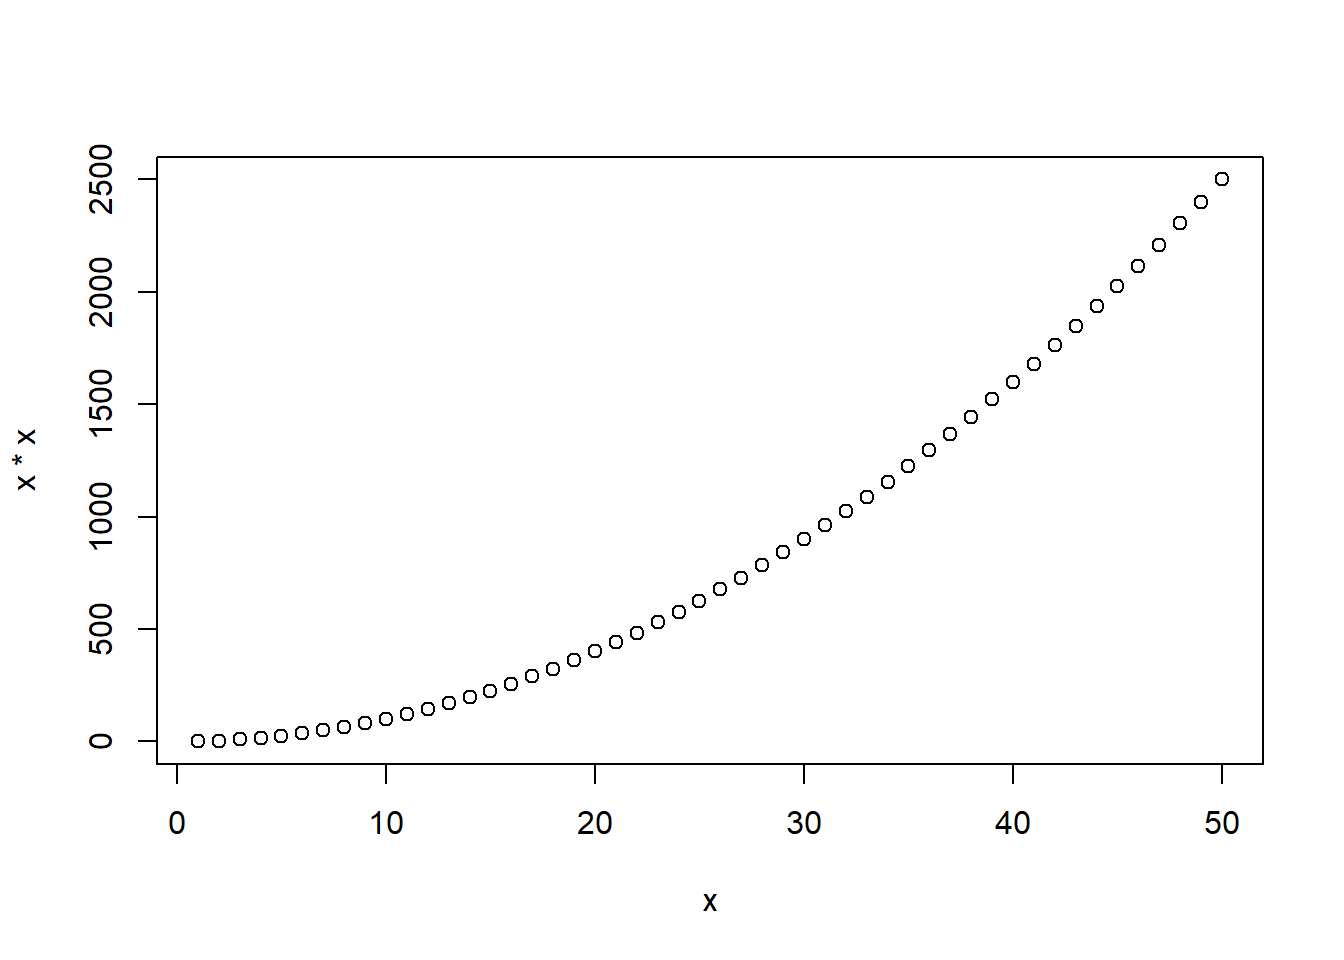
\includegraphics{osnoveR_files/figure-latex/unnamed-chunk-365-1.pdf}

\begin{center}\rule{0.5\linewidth}{\linethickness}\end{center}

Osnovna podrška je funkcionalna i jednostavna, ali ograničena. Na
stvoreni graf se mogu dodavati nove stvari, ali ne i modificirati. Isto
tako, fino podešavanje pojedinih aspekata grafa često pozive čini
glomaznim i nečitljivim te se gubi dimenzija jednostavnosti (koja je
glavni razlog korištenja funkcije plot).

Neki od popularnih paketa za vizualizaciju su \texttt{grid} i
\texttt{lattice}. Paket \texttt{grid} nudi bogatiji skup funkcija za
stvaranje vizualizacija od onih dostupnih unutar osnovne podrške, ali
nema mogućnosti izračuna statistika vezanih uz samu vizualizaciju te je
to često potrebno obaviti ``ručno'' prije pozivanja vizualizacijskih
funkcija. Paket \texttt{lattice} je posebno popularan za stvaranje tzv.
``uvjetnih'' ili ``facetiranih'' grafova (engl. \emph{facet} - aspekt,
značajka), što znači veći broj grafova istog tipa gdje svaki odgovara
pojedinoj vrijednosti neke značajke (npr. usporedba nekih veličina u
nekoj populaciji ovisno o spolu ili dobi). Paket \texttt{lattice}
također ima podršku za automatsko stvaranje legendi i sl. što se kod
drugih paketa često mora raditi ručno. Potencijalni problem ovog paketa
jest činjenica da nije zasnovan ni na kakvom formalnom modelu, tako da
ga je teško proširivati dodatnim funkcionalnostima.

Postoji još popularnih paketa, bilo namijenjenih općenitom stvaranju
vizualizacija ili nekim specifičnim primjenama, no za kraj ćemo
spomenuti jedan od danas najpopularnijih vizualizacijskih paketa jezika
R - paket \texttt{ggplot2}. Autor ovog paketa je već spominjani Hadley
Wickham, a zasnovan je na tzv. ``grafičkoj gramatici'' (zato se i zove
\texttt{ggplot2}, gdje dvojka zapravo dolazi od činjenice da je to paket
za crtanje dvodimenzionalnih vizualizacija).

Popularnost ovog paketa krije se u tome da pokušava objediniti prednosti
osnovne podrške za crtanje grafova kao i paketa \texttt{lattice} ali na
temelju formalnog, jasno definiranog modela. Prednost ovog pristupa jest
ta što omogućuje stvaranje širokog spektra vizualizacija na osnovu
koncizne, jasne i sažete sintakse te omogućuje lako proširenje dodatnim
funkcionalnostima. Potencijalni problem jest nešto strmija inicijalna
krivulja učenja budući da je potrebno prvo usvojiti ``logiku'' stvaranja
grafa, tj. osnovne principe navedene ``grafičke gramatike''. No jednom
kada se premosti ova početna prepreka, stvaranje kvalitetnih
vizualizacija jest brzo, lako i učinkovito, što dokazuje i činjenica da
je \texttt{ggplot2} danas jedan od najpopularnijih paketa za
vizualizaciju podataka koji je izišao iz granica jezika R te se
reimplementira i u drugim programskim jezicima za analizu podataka (npr.
paket \texttt{ggplot} u jeziku \emph{Python}, paket \texttt{gramm} u
\emph{Matlab}-u).

Zbog svega gore navedenog, mi ćemo se u nastavku usredotočiti upravo na
paket \texttt{ggplot2} kao jedan od najpopularnijih i najprimjenjivijih
vizualizacijskih paketa jezika R.

\begin{center}\rule{0.5\linewidth}{\linethickness}\end{center}

\section{\texorpdfstring{Grafička gramatika i paket
\texttt{ggplot2}}{Grafička gramatika i paket ggplot2}}\label{graficka-gramatika-i-paket-ggplot2}

Grafička gramatika (engl. \emph{grammar of graphics}) nam daje sljedeće:

\begin{itemize}
\tightlist
\item
  principe koji omogućuju stvaranje i interpretaciju kompleksnih
  vizualizacija
\item
  naputke što predstavlja ``dobro oblikovanu'' ili ``kvalitetnu''
  vizualizaciju
\end{itemize}

Kao što jezična gramatika omogućuje oblikovanje ``kvalitetnih''
rečenica, tako i grafička gramatika zapravo grafove gleda kao svojevrsne
``rečenice'' čije razumijevanje ovisi o tome kako pojedine komponente
uklopiti u jasnu, razumljivu cjelinu. No, također kao kod jezične
gramatike, rečenica može biti gramatički ispravna ali i dalje besmislena
- drugim riječima, gramatika je temelj za kvalitetu, ali ne i garancija
iste; smislenost i svrhovitost konačnog rezultata i dalje ovisi o
kreativnosti i sposobnosti stvoritelja rečenice, tj. vizualizacije.

Kako bi olakšali učenje grafičke gramatike, što realno predstavlja
najveću prepreku svladavanju paketa \texttt{ggplot2}, važno je da se
pridržavamo osnovnog principa kojeg možemo parafrazirati ovako -
kvalitetna vizualizacija je zapravo kompozicija niza sastavnica od kojih
svaka ima jasno definiranu ulogu. Shodno tome, graf ne bismo trebali
gledati kao jednu kompaktnu cjelinu, već trebamo pokušati identificirati
pojedine dijelove i naučiti na koji način oni doprinose konačnoj
vizualizaciji. Navedeni dijelovi nisu nužno vizualne komponente grafa,
tj. dijelovi koji sačinjavaju grafiku koju gledamo, već gradivni
elementi koje vizualizacijski sustav koristi kako bi stvorio konačni
rezultat.

\begin{center}\rule{0.5\linewidth}{\linethickness}\end{center}

\subsection{Aspekti podataka, estetike i
geometrije}\label{aspekti-podataka-estetike-i-geometrije}

Za početak uvedimo pojednostavljeni model gramatike od tri komponente:

\begin{itemize}
\tightlist
\item
  podaci (koje želimo vizualizirati)
\item
  estetike (mapiranje podataka na elemente grafa)
\item
  geometrije (grafička reprezentacija podataka na grafu)
\end{itemize}

Podaci su, naravno, ključna komponenta grafa. Oni predstavljaju ono što
želimo prikazati grafom. Isto tako, oni su relativno neovisni od ostalih
komponenti vizualizacije - iste principe vizualizacije možemo
primijeniti nad različitim podatkovnim skupovima. No usprkos tome,
stvaranje novog grafa najčešće počinje sa odabirom podatkovnog skupa,
čije značajke diktiraju daljnje korake procesa vizualizacije.

\textbf{Estetike} (engl. \emph{aesthetics}) zapravo nemaju veze sa
doslovnom interpretacijom ``znanosti o lijepom'', već se zapravo radi o
odabiru načina kako određene segmente podatkovnog skupa prikazati na
grafu. Naime da bi vizualizacija podatka imala smisla, mi taj podatak
moramo prikazati na vizualno interpretabilan način. Uobičajen princip
jest prikaz uz pomoć položaja na dvodimenzionalnoj ravnini uz pomoć
kartezijevog koordinatnog sustava koji ravninu ortogonalno segmentira uz
pomoć dvije osi, nazvane \emph{x} i \emph{y}, koje predstavljaju dvije
``osnovne estetike''. One nisu jedine - estetike su također i boja,
oblik, uzorak i sl. Jedan od načina lakšeg razumijevanja što je zapravo
estetika može biti i ``ono što se često objašnjava legendom uz graf'';
ako je estetika zapravo mapiranje na vizualnu komponentu grafa, legenda
grafa je njezin inverz - objašnjenje što koja komponenta zapravo znači.

Konačno, \textbf{geometrija} zapravo predstavlja opis kako konkretno
nacrtati ono što želimo vizualizirati. Na primjer, ako smo mapirali neke
stupce na \emph{x} i \emph{y} os, onda bi se pojedina obzervacija mogla
prikazati točkom, što je tzv. \emph{point geometry}. Mogli smo se isto
tako odlučiti na linijsku geometriju (\emph{line geometry}) i iste
podatke prikazati linijom koja povezuje obzervacije. Geometrija je
zapravo ono što kolokvijalno zovemo ``tip grafa'', tj. crtamo tzv.
``točkaste grafove'' (engl. \emph{scatterplot}), linijske grafove,
stupčaste grafove, pite, histograme i sl. - a sve se to svodi na
dodavanje odgovarajuće ``geometrije'' \texttt{ggplot} grafu.

Svaka geometrija ima svoje parametre koji mogu biti opisani fiksno ili
biti ovisni o podacima - npr. točka ima svojstva položaja (\emph{x} i
\emph{y} koordinate), boje i oblika; točke na grafu možemo npr.
prikazati kružićem, iksićem ili nekim drugim simbolom, a možemo ih
povezati i s nekom estetikom tako da će npr. oblik točke ovisiti o
vrijednosti neke kategorijske varijable. Geometrije se mogu ``slagati''
jedna na drugu tako da isti graf zapravo može biti kombinacija točkastog
i linijskog grafa i sl.

Prikažimo ovo sve na primjeru. Za prve primjere koristit ćemo se
podatkovnim skupom \texttt{mtcars} kojeg smo dobili s osnovnom
distribucijom jezika R unutar paketa \texttt{datasets}. Učitajmo taj
podatkovni skup u globalnu okolinu uz pomoć funkcije \texttt{data}.

\begin{center}\rule{0.5\linewidth}{\linethickness}\end{center}

\textbf{Zadatak 12.2 - upoznavanje sa podatkovnim skupom `mtcars'}

\begin{Shaded}
\begin{Highlighting}[]
\CommentTok{# učitajte podatkovni okvir `mtcars` u globalnu okolinu}

\CommentTok{# proučite okvir `mtcars`  (head, glimpse, ?...)}
\end{Highlighting}
\end{Shaded}

\begin{Shaded}
\begin{Highlighting}[]
\CommentTok{# učitajte podatkovni okvir `mtcars` u globalnu okolinu}
\KeywordTok{data}\NormalTok{(mtcars)}

\CommentTok{# proučite okvir `mtcars`  (head, glimpse, ?...)}
\KeywordTok{glimpse}\NormalTok{(mtcars)}
\KeywordTok{head}\NormalTok{(mtcars)}
\end{Highlighting}
\end{Shaded}

\begin{verbatim}
## Observations: 32
## Variables: 11
## $ mpg  <dbl> 21.0, 21.0, 22.8, 21.4, 18.7, 18.1, 14.3, 24.4, 22.8, 19....
## $ cyl  <dbl> 6, 6, 4, 6, 8, 6, 8, 4, 4, 6, 6, 8, 8, 8, 8, 8, 8, 4, 4, ...
## $ disp <dbl> 160.0, 160.0, 108.0, 258.0, 360.0, 225.0, 360.0, 146.7, 1...
## $ hp   <dbl> 110, 110, 93, 110, 175, 105, 245, 62, 95, 123, 123, 180, ...
## $ drat <dbl> 3.90, 3.90, 3.85, 3.08, 3.15, 2.76, 3.21, 3.69, 3.92, 3.9...
## $ wt   <dbl> 2.620, 2.875, 2.320, 3.215, 3.440, 3.460, 3.570, 3.190, 3...
## $ qsec <dbl> 16.46, 17.02, 18.61, 19.44, 17.02, 20.22, 15.84, 20.00, 2...
## $ vs   <dbl> 0, 0, 1, 1, 0, 1, 0, 1, 1, 1, 1, 0, 0, 0, 0, 0, 0, 1, 1, ...
## $ am   <dbl> 1, 1, 1, 0, 0, 0, 0, 0, 0, 0, 0, 0, 0, 0, 0, 0, 0, 1, 1, ...
## $ gear <dbl> 4, 4, 4, 3, 3, 3, 3, 4, 4, 4, 4, 3, 3, 3, 3, 3, 3, 4, 4, ...
## $ carb <dbl> 4, 4, 1, 1, 2, 1, 4, 2, 2, 4, 4, 3, 3, 3, 4, 4, 4, 1, 2, ...
##                    mpg cyl disp  hp drat    wt  qsec vs am gear carb
## Mazda RX4         21.0   6  160 110 3.90 2.620 16.46  0  1    4    4
## Mazda RX4 Wag     21.0   6  160 110 3.90 2.875 17.02  0  1    4    4
## Datsun 710        22.8   4  108  93 3.85 2.320 18.61  1  1    4    1
## Hornet 4 Drive    21.4   6  258 110 3.08 3.215 19.44  1  0    3    1
## Hornet Sportabout 18.7   8  360 175 3.15 3.440 17.02  0  0    3    2
## Valiant           18.1   6  225 105 2.76 3.460 20.22  1  0    3    1
\end{verbatim}

\begin{center}\rule{0.5\linewidth}{\linethickness}\end{center}

Vidimo da ovi podaci opisuju karakteristike 32 (stara) automobila kao
što su: težina, maksimalna brzina, broj konjskih snaga, broj cilindara i
sl.

Kada stvaramo \texttt{ggplot2} vizualizaciju onda često pomaže da
razmišljamo o ``slojevima'' grafa. Svaki sloj na neki način ``prekriva''
graf poput prozirne folije, što nam omogućuje postavljanje više
različitih tipova reprezentacije podataka na isti graf (npr. prikazujemo
točke ali ih i povežemo linijom).

Recimo da nas zanima kako se odnose težina automobila i njegova
maksimalna brzina. Intuitivni način vizualizacije bio bi:

\begin{itemize}
\tightlist
\item
  težina automobila (\texttt{wt}) na x os grafa
\item
  potrošnja (\texttt{mpg}) na y os grafa
\end{itemize}

Pogledajmo kako ovo izvesti uz pomoć \texttt{ggplot2} vizualizacije.
Uočimo da ćemo za početak namjerno koristiti ``opširan'' način stvaranja
grafa - ovakav način se gotovo nikad ne koristi u praksi budući da
postoji puno podesniji, sažeti način poziva metode, no na ovaj način
lako ćemo uočiti pojedine bitne elemente izgradnje grafa. Stvorimo tzv.
``točkasti'' graf (engl. \emph{scatterplot}) koji pokazuje odnos težine
i maksimalne brzine automobila opisanih tablicom \texttt{mtcars}.

\begin{center}\rule{0.5\linewidth}{\linethickness}\end{center}

\subsubsection{\texorpdfstring{Prvi \texttt{ggplot2}
graf}{Prvi ggplot2 graf}}\label{prvi-ggplot2-graf}

\begin{Shaded}
\begin{Highlighting}[]
\KeywordTok{ggplot}\NormalTok{() }\OperatorTok{+}\StringTok{ }
\KeywordTok{layer}\NormalTok{( }\DataTypeTok{data =}\NormalTok{ mtcars,                      }\CommentTok{# 1. podaci}
       \DataTypeTok{mapping =} \KeywordTok{aes}\NormalTok{(}\DataTypeTok{x =}\NormalTok{ wt, }\DataTypeTok{y =}\NormalTok{ mpg),     }\CommentTok{# 2. mapiranja / estetike}
       \DataTypeTok{geom =} \StringTok{"point"}\NormalTok{,                     }\CommentTok{# 3. geometrija}
       \DataTypeTok{stat =} \StringTok{"identity"}\NormalTok{,                  }\CommentTok{# za sada zanemariti}
       \DataTypeTok{position =} \StringTok{"identity"}\NormalTok{)              }\CommentTok{# za sada zanemariti}
\end{Highlighting}
\end{Shaded}

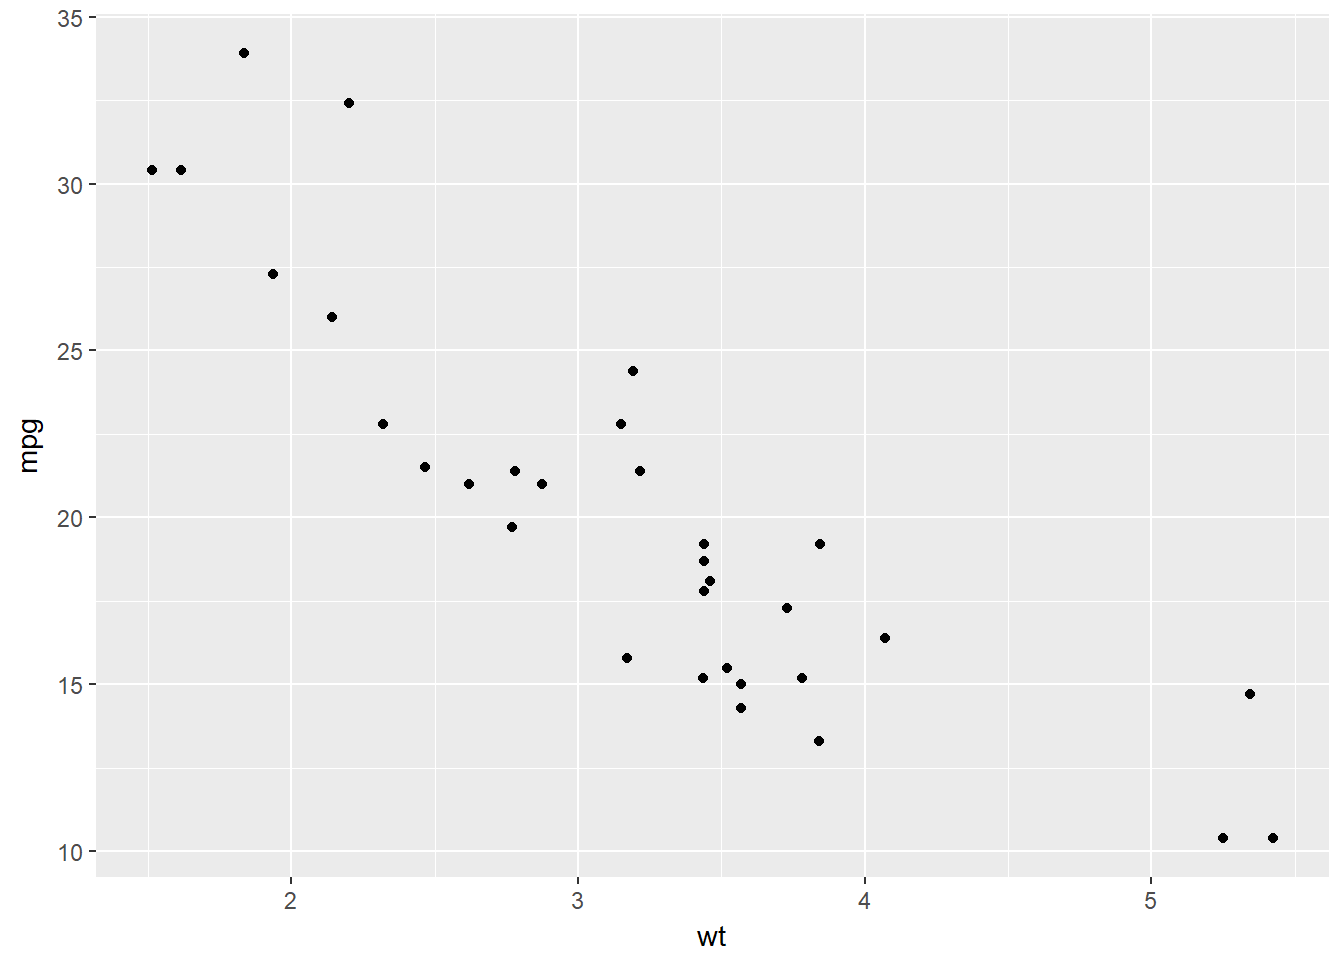
\includegraphics{osnoveR_files/figure-latex/unnamed-chunk-368-1.pdf}

Osnovna funkcija za izgradnju jest funkcija \texttt{ggplot}. Ona zapravo
inicijalizira objekt klase \texttt{ggplot}. Naime, za \texttt{ggplot2}
vizualizacije specifično je da su grafovi zapravo objekti, a ono što
inače smatramo grafom je samo njihova vizualna reprezentacija. Ovdje
zapravo leži moć ovakvog tipa reprezentacija - graf je nešto što možemo
po volji mijenjati, preoblikovati, proširivati i pohranjivati, a
vizualizacija predstavlja konačni nusproizvod upravljanja tim objektom.

Ovakvom objektu potom dodajemo ``slojeve'' uz pomoć funkcije
\texttt{layer}. Sloj objektu dodajemo uz pomoć operatora \texttt{+}, što
predstavlja intuitivan prikaz i olakšava rad sa ovakvim tipom grafova.
Sloj kao takav ima one gramatičke aspekte o kojima smo ranije govorili -
podatke, estetike i geometrije. U pozivu vidimo još dva aspekta grafičke
gramatike - statistike i poziciju - koje ćemo objasniti kasnije.
Dovoljno je napomenuti da \texttt{"identity"} zapravo znači ``ostavi
onako kakvo jest'', tj. radi se o nekoj dodatnoj obradi unutar procesa
vizualizacije koju za sada zanemarujemo, tj. ne koristimo.

Iako formalno svaki sloj ima svoje gramatičke aspekte, gotovo uvijek
postoje aspekti koji su zajednički svim slojevima (npr. vrlo često jedan
graf prikazuje jedan podatkovni skup a svi slojevi ``dijele'' x i y os).
Ukoliko imamo ovakve zajedničke aspekte onda ih možemo definirati odmah
kod stvaranja objekta \texttt{ggplot} koji onda postaju ``default-ni''
parametri slojeva koje dodajemo (iako oni uvijek imaju opciju
``gaženja'' tih parametara svojim aspektima). Isto tako, za stvaranje
dodatnih slojeva često se koristimo pomoćnim funkcijama intuitivnog
imena koje imaju unaprijed podešene najčešće korištene parametre kako ih
ne bismo morali stalno ponovo upisivati. Tako npr. funkcija
\texttt{geom\_point} dodaje sloj koji nasljeđuje već definirane aspekte
a kao geometriju koristi točke.

Pogledajmo sljedeći primjer koji koristi ``skraćeni'' način stvaranja
navedenog grafa:

\begin{Shaded}
\begin{Highlighting}[]
\CommentTok{# prvi `ggplot2` graf, skraćeni način izgradnje grafa}
\KeywordTok{ggplot}\NormalTok{(mtcars, }\KeywordTok{aes}\NormalTok{(}\DataTypeTok{x =}\NormalTok{ wt, }\DataTypeTok{y =}\NormalTok{ mpg)) }\OperatorTok{+}\StringTok{ }\KeywordTok{geom_point}\NormalTok{()}
\end{Highlighting}
\end{Shaded}

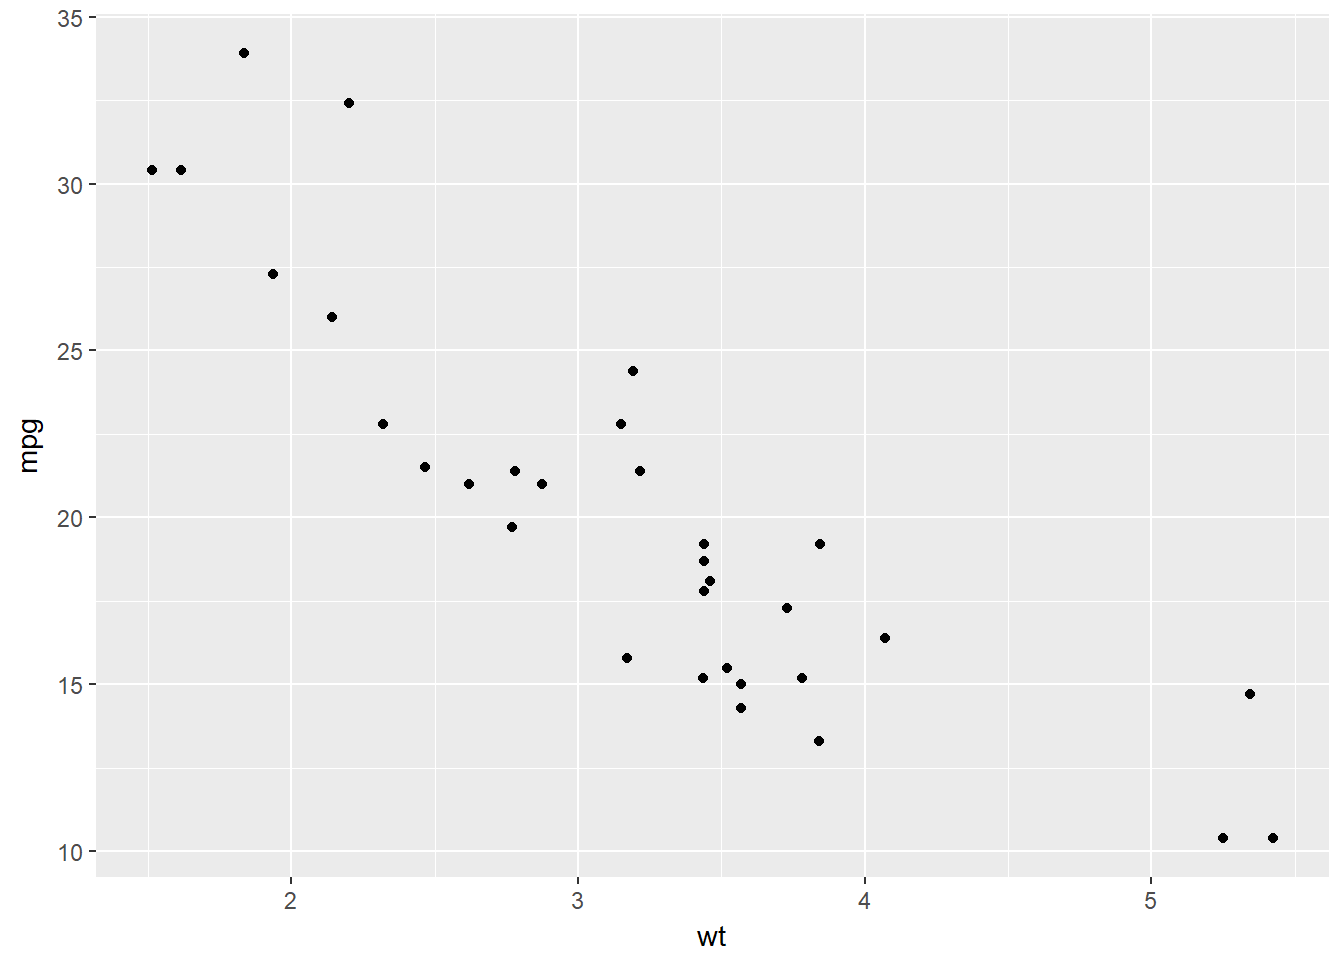
\includegraphics{osnoveR_files/figure-latex/unnamed-chunk-369-1.pdf}

Postoji još jedan ``pojednostavljeni'' način stvaranja \texttt{ggplot}
grafova, a to je uz pomoć funkcije \texttt{qplot} (od ``*quick plot``).
Ova funkcija zapravo je omotač koji omogućuje da \texttt{ggplot} grafove
stvaramo sintaksom vrlo sličnom sintaksi funkcije \texttt{plot}.

\begin{Shaded}
\begin{Highlighting}[]
\CommentTok{# prvi `ggplot2` graf, funkcija `qplot`}
\KeywordTok{qplot}\NormalTok{(}\DataTypeTok{x =}\NormalTok{ wt, }\DataTypeTok{y =}\NormalTok{ mpg, }\DataTypeTok{data =}\NormalTok{ mtcars)}
\end{Highlighting}
\end{Shaded}

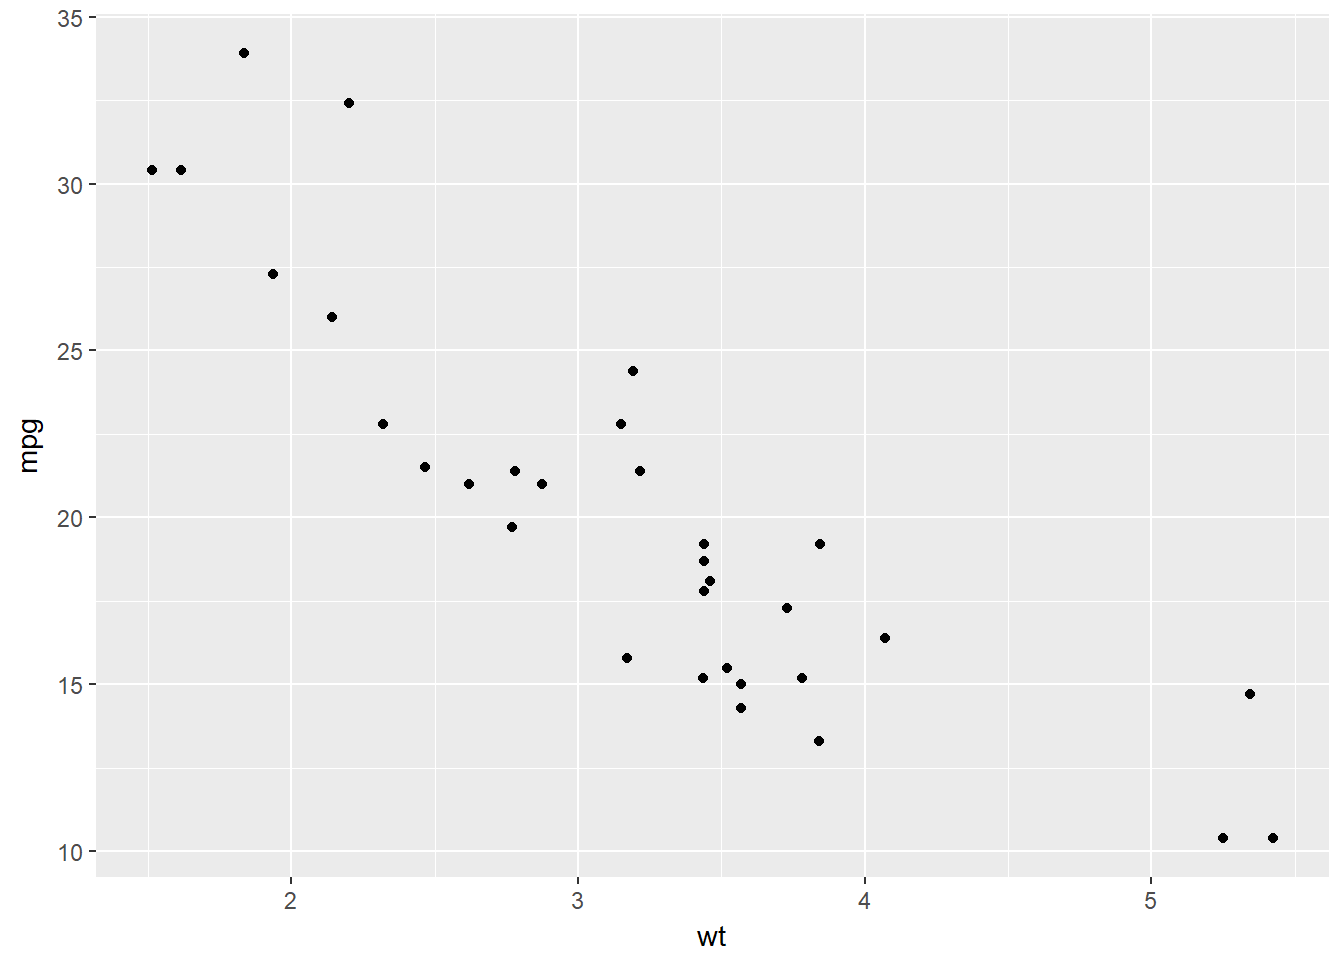
\includegraphics{osnoveR_files/figure-latex/unnamed-chunk-370-1.pdf}

Glavni razlog postojanja ove funkcije jest orijentiranost korisnicima
koji traže brzu i učinkovitu alternativu \texttt{plot} funkciji bez
potrebe za učenjem novih koncepata. Iako se možda ovakav način stvaranja
grafova možda čini zgodan i jednostavan, dugoročno se ipak isplati
naučiti ``pravu'' \emph{ggplot2} sintaksu budući da je \texttt{qplot}
funkcija dosta limitirana i - poput funkcije \texttt{plot} - inicijalna
jednostavnost se sve više gubi što više prilagodbi vizualizacije želimo
provesti.

Vratimo se sada na naš graf - što ako želimo na njemu prikazati dodatni
stupac tj. varijablu? Npr. možemo vidjeti da svi auti imaju 4, 6 ili 8
cilindara, što znači da se ova varijabla može tretirati i kao
kategorijska, tj. možemo ju faktorizirati. No graf koji imamo je
dvodimenzionalan - kako dodati ``treću dimenziju''? Odgovor je -
koristimo neku dosad neiskorištenu estetiku, npr. boju, veličinu ili
oblik točaka.

Dodajte broj cilindara u gornji graf. Koristite \texttt{ggplot} funkciju
i \texttt{shape} ili \texttt{color} estetiku kojoj ćete pridružiti
varijablu \texttt{cyl}. Prije stvaranja grafa faktorizirajte varijablu
\texttt{cyl}.

\begin{center}\rule{0.5\linewidth}{\linethickness}\end{center}

\textbf{Zadatak 12.3 - `shape' estetika}

\begin{Shaded}
\begin{Highlighting}[]
\CommentTok{# stvorite `ggplot` graf skupa `mtcars` sa mapiranjima:  x = wt, y = mpg, shape = cyl}
\CommentTok{# koristite geometriju točke}
\CommentTok{# što se događa ako zaboravimo faktorizirati stupac `cyl`?}
\end{Highlighting}
\end{Shaded}

\begin{Shaded}
\begin{Highlighting}[]
\NormalTok{mtcars}\OperatorTok{$}\NormalTok{cyl <-}\StringTok{ }\KeywordTok{as.factor}\NormalTok{(mtcars}\OperatorTok{$}\NormalTok{cyl)}

\KeywordTok{ggplot}\NormalTok{(mtcars, }\KeywordTok{aes}\NormalTok{(}\DataTypeTok{x =}\NormalTok{ wt, }\DataTypeTok{y =}\NormalTok{ mpg, }\DataTypeTok{shape =}\NormalTok{ cyl)) }\OperatorTok{+}\StringTok{ }\KeywordTok{geom_point}\NormalTok{()}
\end{Highlighting}
\end{Shaded}

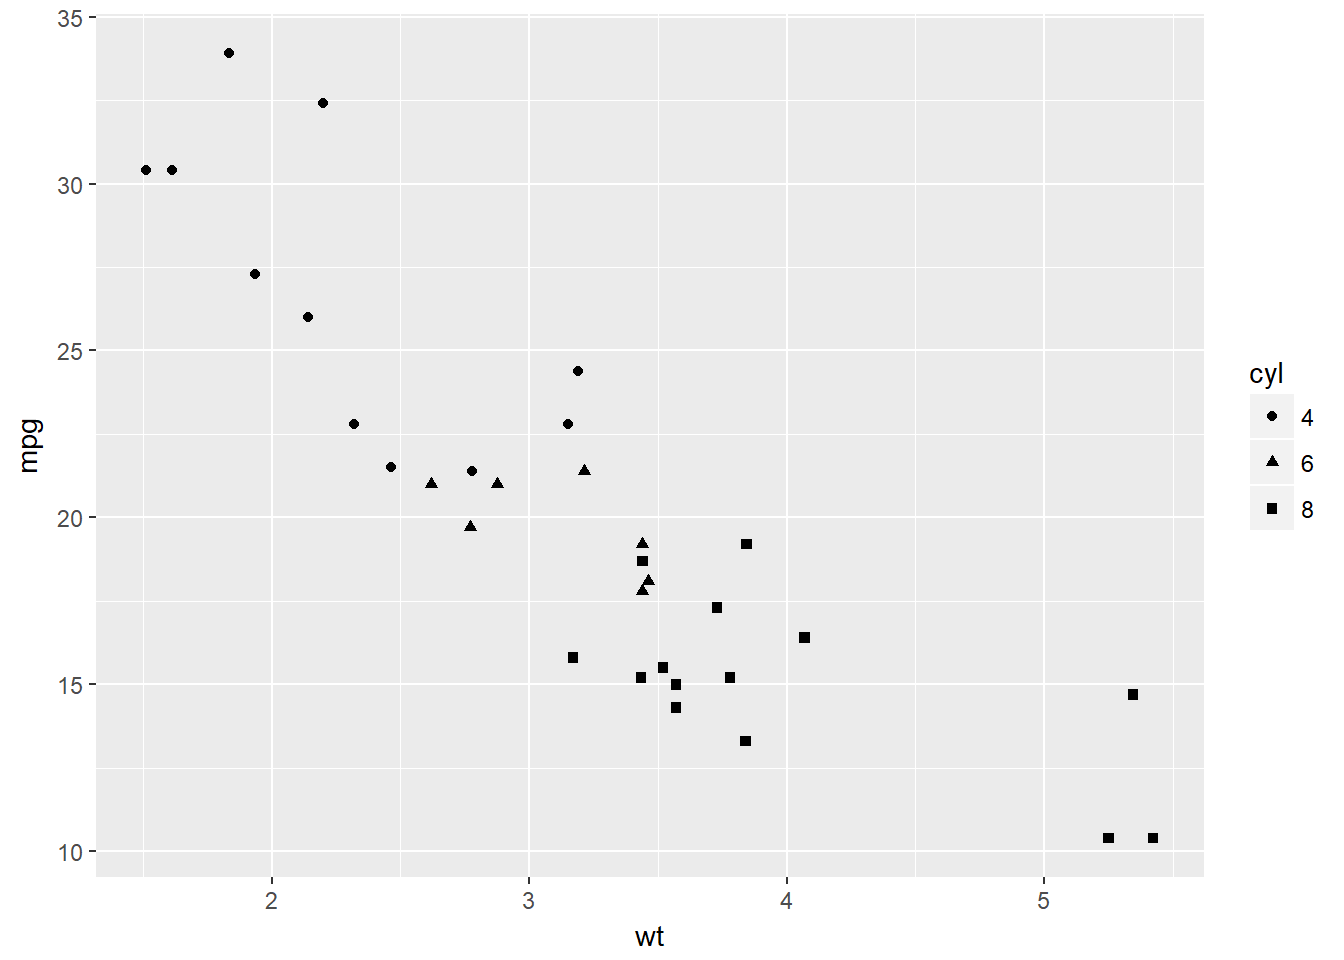
\includegraphics{osnoveR_files/figure-latex/unnamed-chunk-372-1.pdf}

\begin{center}\rule{0.5\linewidth}{\linethickness}\end{center}

\textbf{Zadatak 12.4 - `color' estetika}

\begin{Shaded}
\begin{Highlighting}[]
\CommentTok{# ponovite isti graf, ali umjesto estetike `shape` koristite estetiku `color`}
\end{Highlighting}
\end{Shaded}

\begin{Shaded}
\begin{Highlighting}[]
\KeywordTok{ggplot}\NormalTok{(mtcars, }\KeywordTok{aes}\NormalTok{(}\DataTypeTok{x =}\NormalTok{ wt, }\DataTypeTok{y =}\NormalTok{ mpg, }\DataTypeTok{color =}\NormalTok{ cyl)) }\OperatorTok{+}\StringTok{ }\KeywordTok{geom_point}\NormalTok{()}
\end{Highlighting}
\end{Shaded}

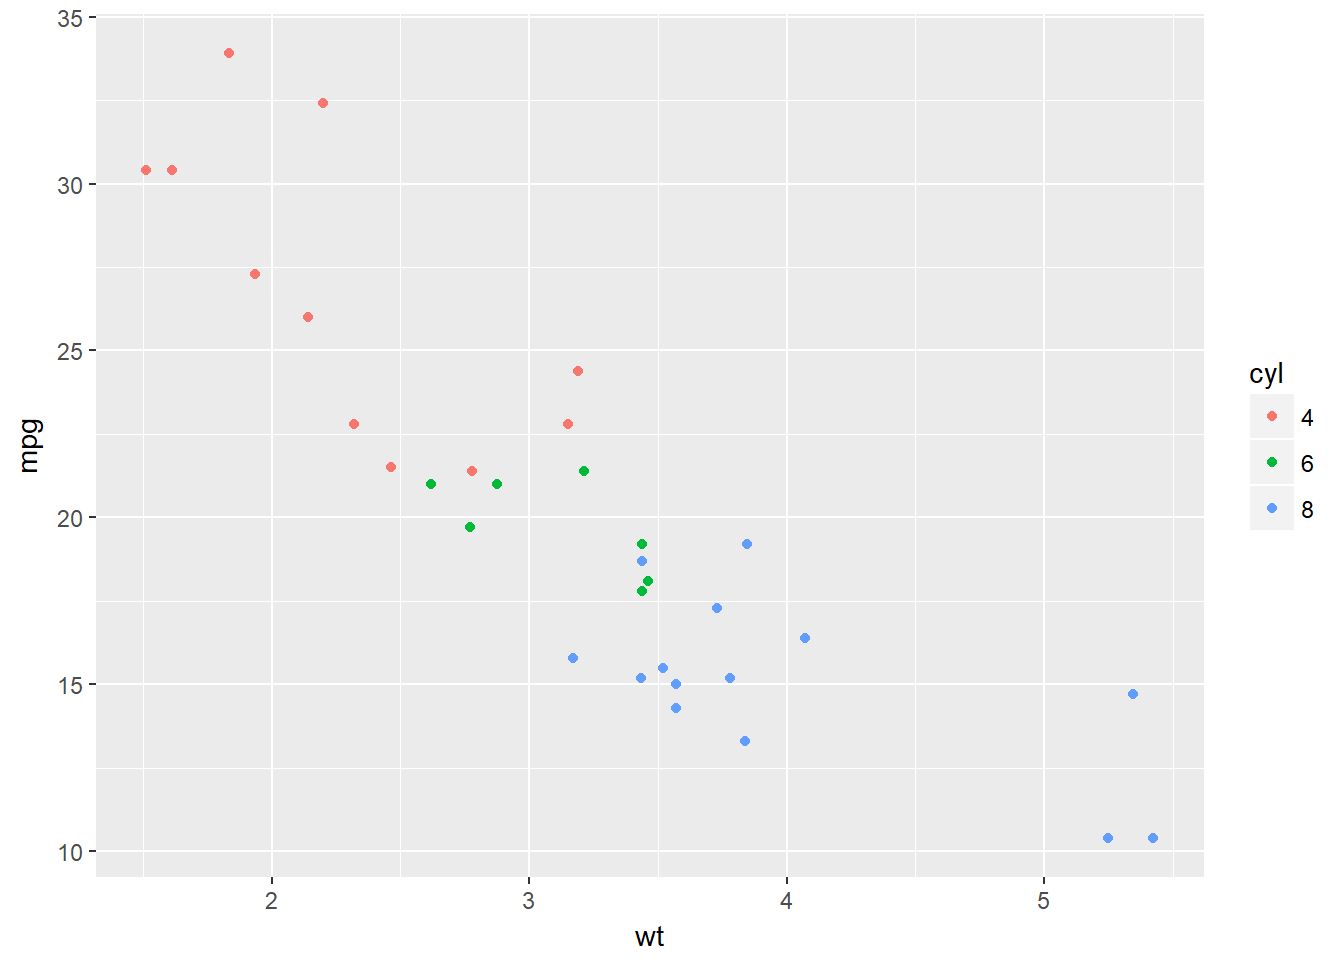
\includegraphics{osnoveR_files/figure-latex/unnamed-chunk-374-1.pdf}

\begin{center}\rule{0.5\linewidth}{\linethickness}\end{center}

\textbf{Zadatak 12.5 - 1.5 - kombiniranje estetika}

\begin{Shaded}
\begin{Highlighting}[]
\CommentTok{# ponovite isti graf, ali sada za `cyl` stupac kombinirajte i `shape` i `color` estetiku}
\end{Highlighting}
\end{Shaded}

\begin{Shaded}
\begin{Highlighting}[]
\KeywordTok{ggplot}\NormalTok{(mtcars, }\KeywordTok{aes}\NormalTok{(}\DataTypeTok{x =}\NormalTok{ wt, }\DataTypeTok{y =}\NormalTok{ mpg, }\DataTypeTok{color =}\NormalTok{ cyl, }\DataTypeTok{shape =}\NormalTok{ cyl)) }\OperatorTok{+}\StringTok{ }\KeywordTok{geom_point}\NormalTok{()}
\end{Highlighting}
\end{Shaded}

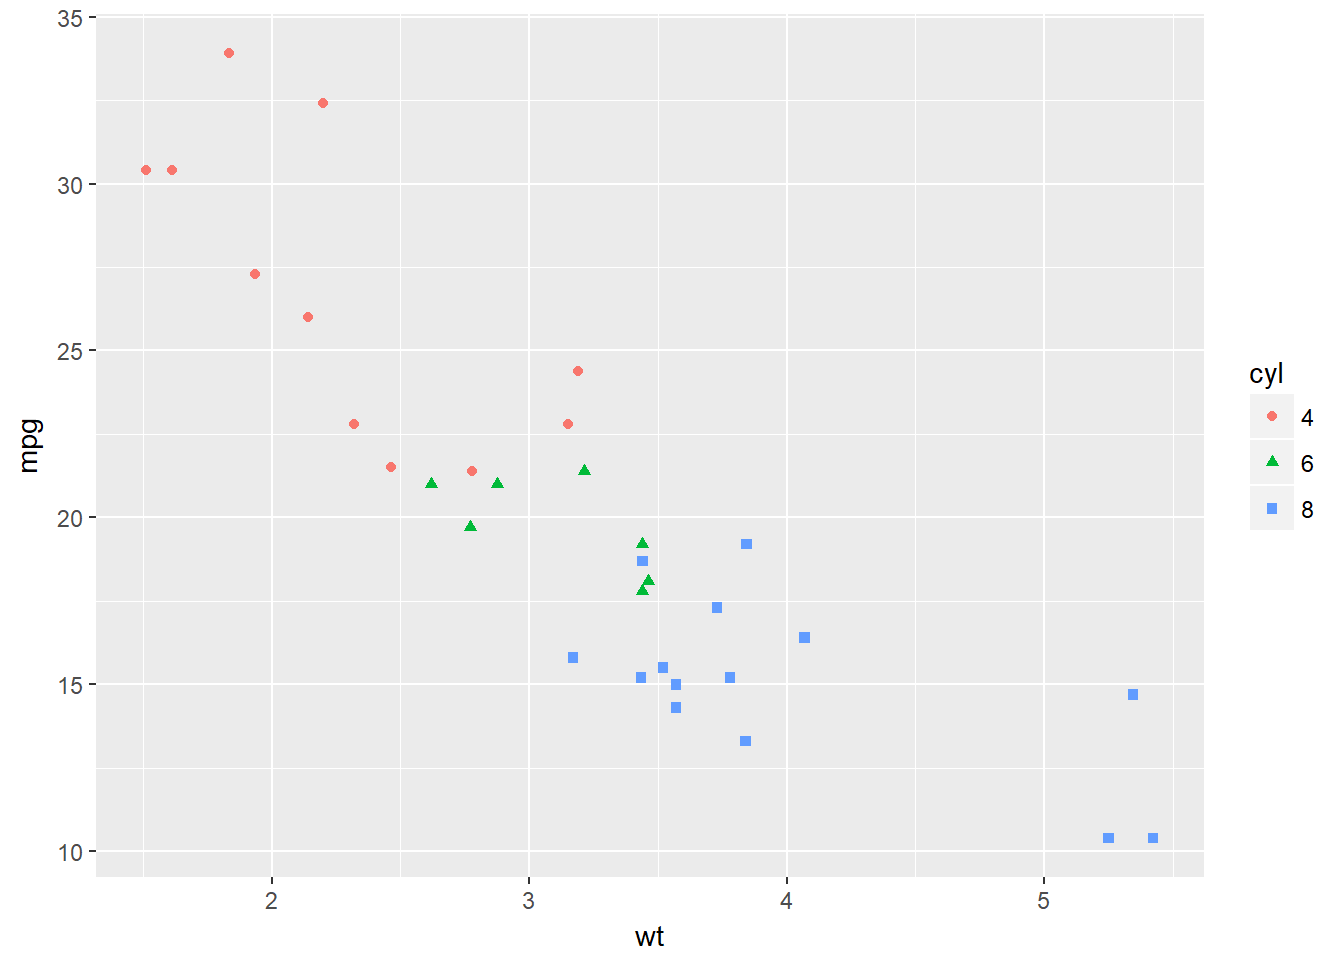
\includegraphics{osnoveR_files/figure-latex/unnamed-chunk-376-1.pdf}

\begin{center}\rule{0.5\linewidth}{\linethickness}\end{center}

Usporedbom grafova možemo zaključiti da je boju puno lakše vizualno
interpetirati od oblika, što znači da je ona često preferirana estetika
(ali nije primjerena ako nam grafovi moraju biti crno-bijeli). Isto
tako, uočite da možemo lako kombinirati dvije estetike nad istom
varijablom, ukoliko želimo.

\begin{center}\rule{0.5\linewidth}{\linethickness}\end{center}

\subsubsection{\texorpdfstring{Funkcija
\texttt{labs}}{Funkcija labs}}\label{funkcija-labs}

Vidjeli smo kako \texttt{ggplot} automatski stvara legendu za svoje
estetike te da imenuje osi imenom varijable (osi \emph{x} i \emph{y}
također možemo smatrati svojevrsnim ``legendama''). Ukoliko želimo ručno
imenovati osi i legende, ali i dodati naslov grafu možemo se poslužiti
funkcijom \texttt{labs} koju također dodajemo kao novi sloj i koja može
imati sljedeću sintaksu:

\begin{Shaded}
\begin{Highlighting}[]
\KeywordTok{ggplot}\NormalTok{(... ) }\OperatorTok{+}\StringTok{ }\NormalTok{...}

\OperatorTok{+}\StringTok{ }\KeywordTok{labs}\NormalTok{(}\DataTypeTok{x =} \StringTok{"x os"}\NormalTok{, }\DataTypeTok{y =} \StringTok{"y os"}\NormalTok{, }\DataTypeTok{title =} \StringTok{"Naslov"}\NormalTok{)}
\end{Highlighting}
\end{Shaded}

Isprobajmo ovo na primjeru.

\textbf{Zadatak 12.6 - funkcija `labs'}

\begin{Shaded}
\begin{Highlighting}[]
\CommentTok{# na sljedećem grafu preimenujte osi i legendu}
\CommentTok{# te dodajte adekvatni naslov (najbolje nešto što objašnjava graf)}
\KeywordTok{ggplot}\NormalTok{(mtcars, }\KeywordTok{aes}\NormalTok{(}\DataTypeTok{x =}\NormalTok{ wt, }\DataTypeTok{y =}\NormalTok{ mpg, }\DataTypeTok{color =}\NormalTok{ cyl, }\DataTypeTok{shape =}\NormalTok{ cyl)) }\OperatorTok{+}\StringTok{ }\KeywordTok{geom_point}\NormalTok{() }
\end{Highlighting}
\end{Shaded}

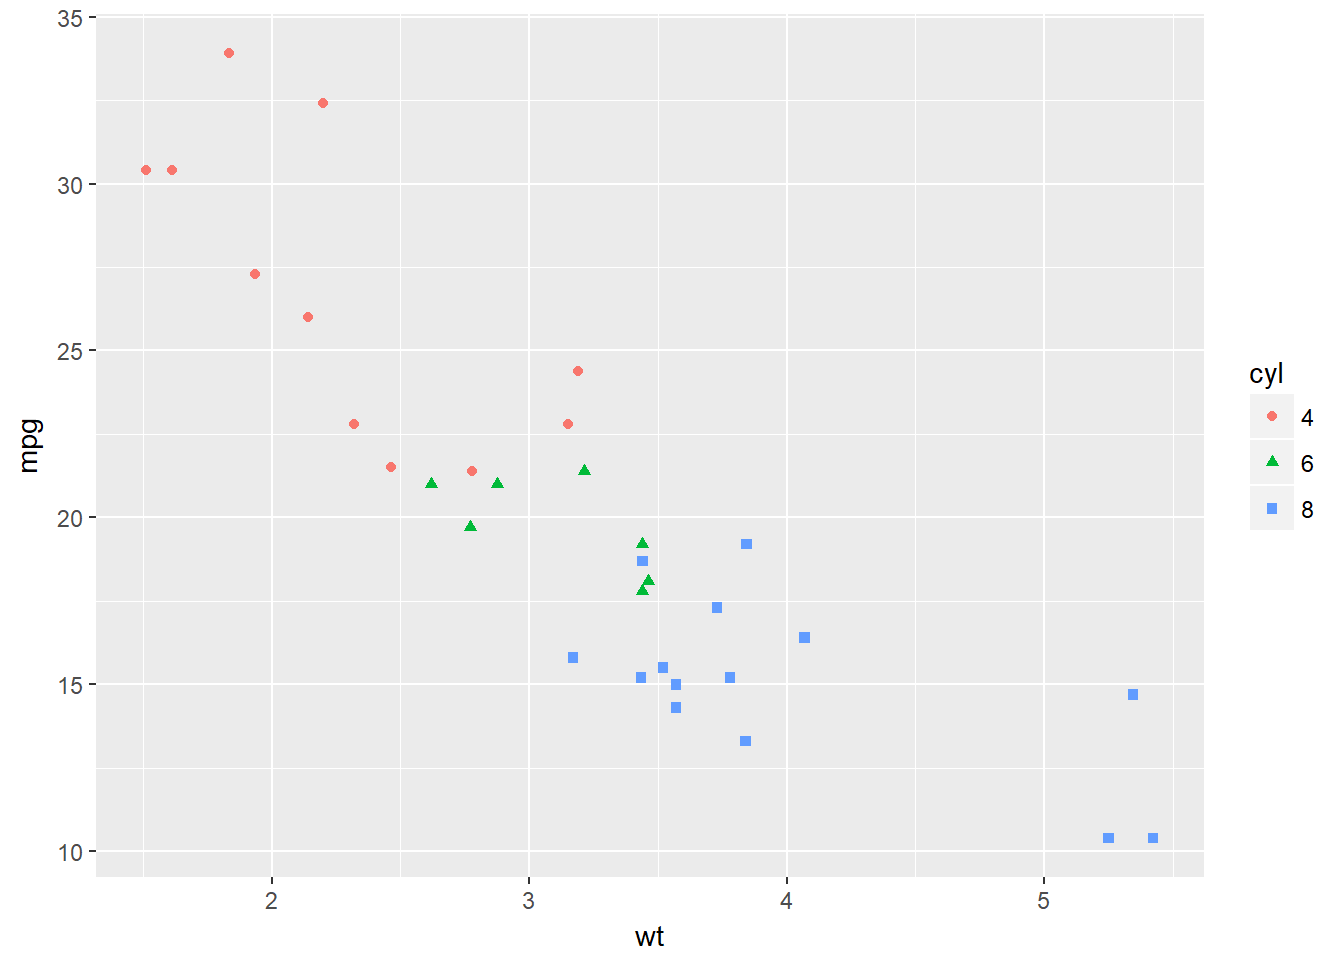
\includegraphics{osnoveR_files/figure-latex/unnamed-chunk-378-1.pdf}

\begin{Shaded}
\begin{Highlighting}[]
\CommentTok{# na sljedećem grafu preimenujte osi i legendu}
\CommentTok{# te dodajte adekvatni naslov (najbolje nešto što objašnjava graf)}
\KeywordTok{ggplot}\NormalTok{(mtcars, }\KeywordTok{aes}\NormalTok{(}\DataTypeTok{x =}\NormalTok{ wt, }\DataTypeTok{y =}\NormalTok{ mpg, }\DataTypeTok{color =}\NormalTok{ cyl, }\DataTypeTok{shape =}\NormalTok{ cyl)) }\OperatorTok{+}\StringTok{ }\KeywordTok{geom_point}\NormalTok{() }\OperatorTok{+}
\KeywordTok{labs}\NormalTok{(}\DataTypeTok{x =} \StringTok{"Težina / 1000 lb"}\NormalTok{, }\DataTypeTok{y =} \StringTok{"Potrošnja / milja po galonu"}\NormalTok{,}
     \DataTypeTok{color =} \StringTok{"Broj cilindara"}\NormalTok{, }\DataTypeTok{shape =} \StringTok{"Broj cilindara"}\NormalTok{,}
   \DataTypeTok{title =} \StringTok{"Teži auti više troše (manje milja na jedan galon benzina)"}\NormalTok{)}
\end{Highlighting}
\end{Shaded}

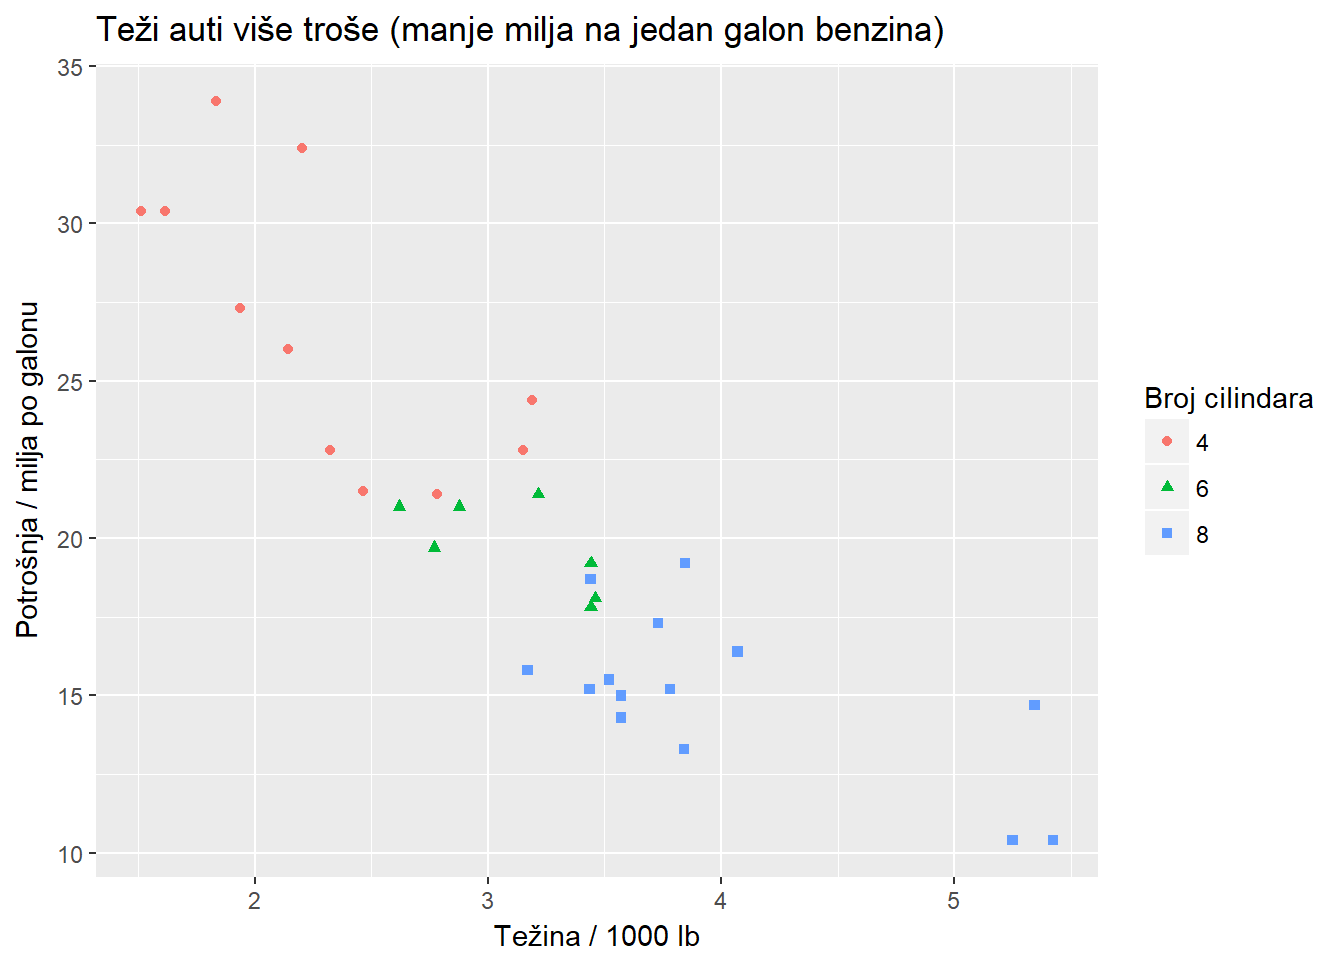
\includegraphics{osnoveR_files/figure-latex/unnamed-chunk-379-1.pdf}

\begin{center}\rule{0.5\linewidth}{\linethickness}\end{center}

\subsection{Fiksni parametri
geometrije}\label{fiksni-parametri-geometrije}

Prije nastavka, obratimo pažnju na jednu prilično važnu stvar koju do
sada nismo razjasnili: što kada želimo utjecati na određene parametre
odabrane geometrije, ali želimo ih odrediti fiksno, umjesto da budu
povezani sa određenom estetikom, tj. mapiranjem na određenu varijablu?
Ili, konkretno - što ako želim napraviti graf ovisnosti maksimalne
brzine o težini automobila, ali želim da graf ima točke crvene boje, ili
oblika ``X'' - tj. da su boja i oblik fiksni, umjesto da ovise o nekoj
varijabli? Odgovor je zapravo vrlo jednostavan - umjesto da za parametar
postavimo ime varijable (npr. \texttt{wt}), mi ga inicijaliziramo na
znakovnu ili numeričku vrijednost koja je smislena za taj parametar
(npr. \texttt{"red"} ili \texttt{"\#FF0000"} za boju, broj od 0 do 25 za
oblik).

Primjer sintakse:

\begin{Shaded}
\begin{Highlighting}[]
\KeywordTok{ggplot}\NormalTok{(mtcars, }\KeywordTok{aes}\NormalTok{(wt, mpg)) }\OperatorTok{+}\StringTok{ }\KeywordTok{geom_point}\NormalTok{(}\DataTypeTok{color =} \StringTok{"blue"}\NormalTok{)}
\end{Highlighting}
\end{Shaded}

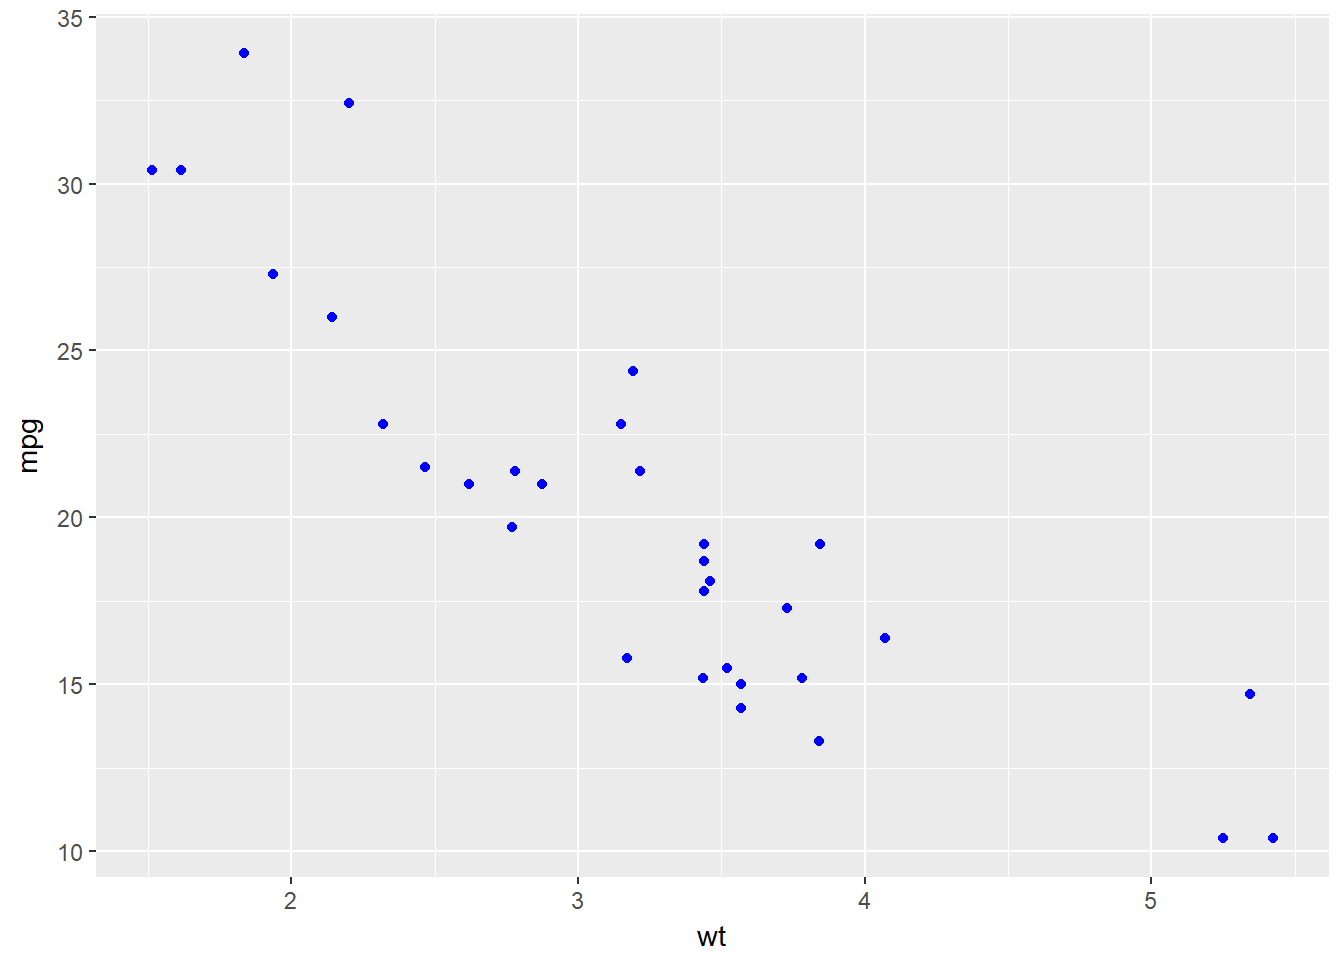
\includegraphics{osnoveR_files/figure-latex/unnamed-chunk-380-1.pdf}

Primjer \textbf{krive} sintakse:

\begin{Shaded}
\begin{Highlighting}[]
\CommentTok{# ggplot će raditi mapiranje riječi "blue" na estetiku `color`}
\KeywordTok{ggplot}\NormalTok{(mtcars, }\KeywordTok{aes}\NormalTok{(wt, mpg)) }\OperatorTok{+}\StringTok{ }\KeywordTok{geom_point}\NormalTok{(}\KeywordTok{aes}\NormalTok{(}\DataTypeTok{color =} \StringTok{"blue"}\NormalTok{))}
\end{Highlighting}
\end{Shaded}

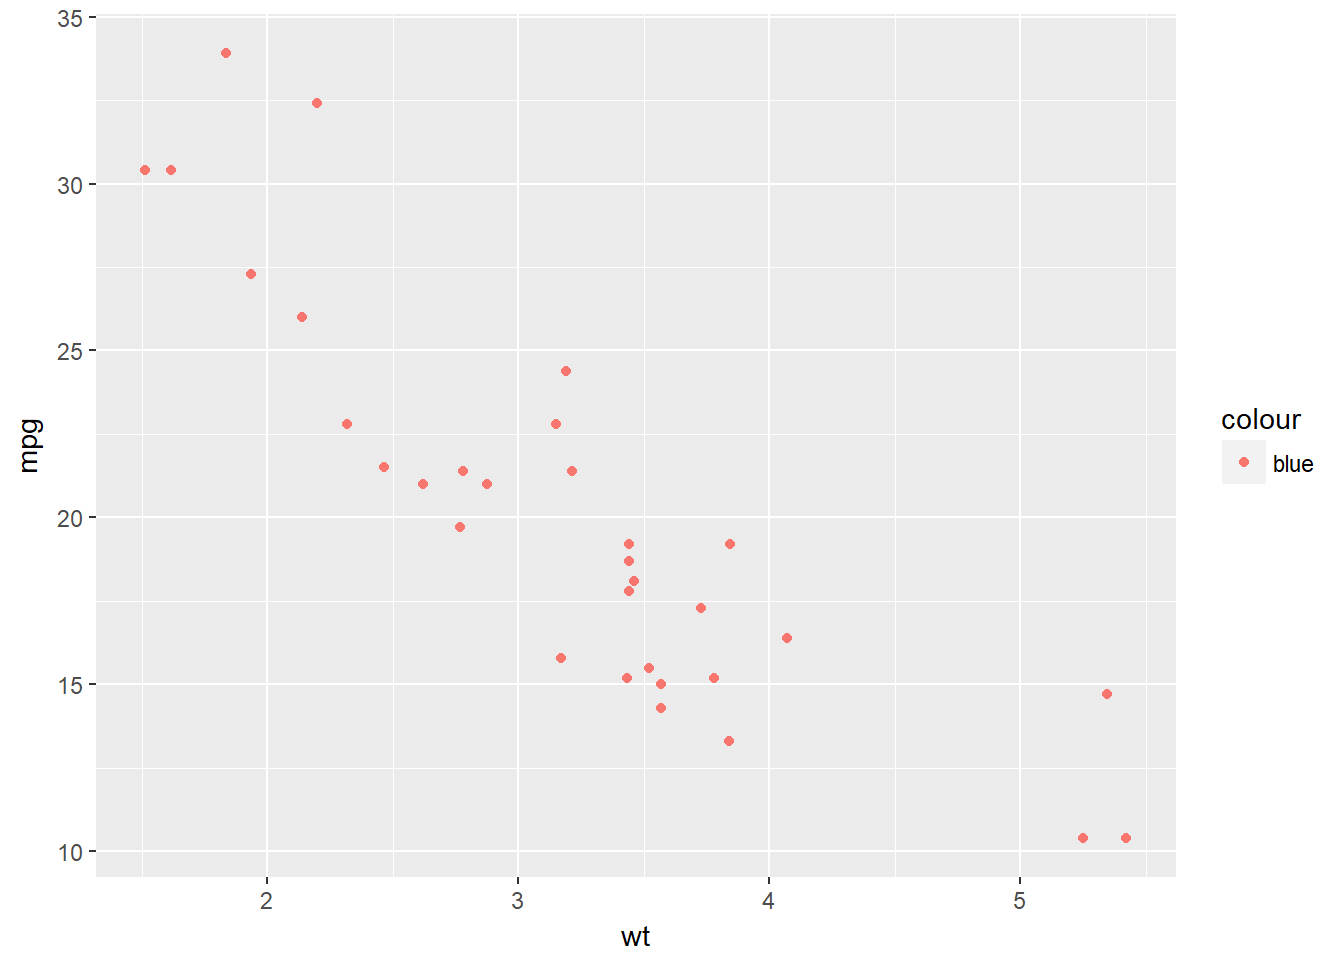
\includegraphics{osnoveR_files/figure-latex/unnamed-chunk-381-1.pdf}

Pokušajte ovo primijeniti na primjeru.

\begin{center}\rule{0.5\linewidth}{\linethickness}\end{center}

\textbf{Zadatak 12.7 - fiksni parametri geometrije}

\begin{Shaded}
\begin{Highlighting}[]
\CommentTok{# nacrtajte graf ovisnosti maksimalne brzine o težini automobila}
\CommentTok{# koristite geometriju točke}
\CommentTok{# točke neka budu crvene boje, neka oblik broj 4 (iksić) i veličinu 3}
\end{Highlighting}
\end{Shaded}

\begin{Shaded}
\begin{Highlighting}[]
\KeywordTok{ggplot}\NormalTok{(mtcars, }\KeywordTok{aes}\NormalTok{(}\DataTypeTok{x =}\NormalTok{ wt, }\DataTypeTok{y =}\NormalTok{ mpg)) }\OperatorTok{+}\StringTok{ }\KeywordTok{geom_point}\NormalTok{(}\DataTypeTok{color =} \StringTok{"red"}\NormalTok{, }\DataTypeTok{shape =} \DecValTok{4}\NormalTok{, }\DataTypeTok{size =} \DecValTok{3}\NormalTok{)}
\end{Highlighting}
\end{Shaded}

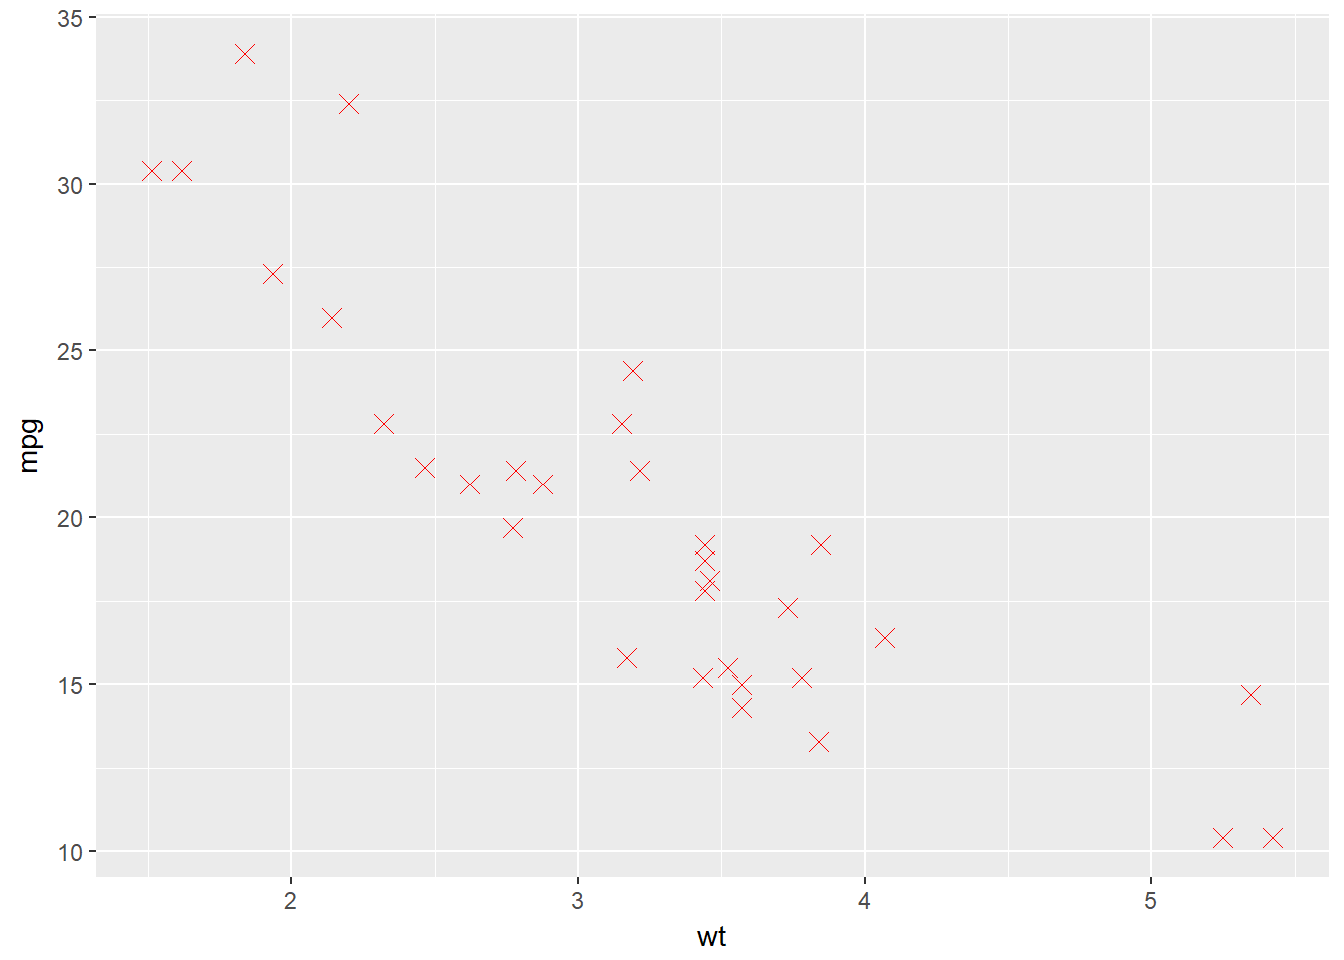
\includegraphics{osnoveR_files/figure-latex/unnamed-chunk-383-1.pdf}

\begin{center}\rule{0.5\linewidth}{\linethickness}\end{center}

\subsection{Aspekti statistike i
pozicije}\label{aspekti-statistike-i-pozicije}

Vratimo se sada na prvi graf koji je uspoređivao težinu i maksimalnu
brzinu. Što ako smo htjeli ovu povezanost prikazati linijom? Pokušajte
donjem pozivu dodati sloj koji koristi postojeće aspekte, ali koristi
linijsku geometriju. Možete koristiti funkciju \texttt{layer} sa
postavljenim \texttt{geom} parametrom na \texttt{"line"}, no popularniji
pristup je korištenje pomoćne funkcije \texttt{geom\_line} koja radi
slično kao funkcija \texttt{geom\_point}.

\begin{center}\rule{0.5\linewidth}{\linethickness}\end{center}

\textbf{Zadatak 12.8 - dodavanje linijskog sloja}

\begin{Shaded}
\begin{Highlighting}[]
\CommentTok{# budući da stalno koristimo istu "osnovicu" grafa možemo ju}
\CommentTok{# pohraniti u zasebnu varijablu npr. imena `graf`}

\NormalTok{graf <-}\StringTok{ }\KeywordTok{ggplot}\NormalTok{(mtcars, }\KeywordTok{aes}\NormalTok{(}\DataTypeTok{x =}\NormalTok{ wt, }\DataTypeTok{y =}\NormalTok{ mpg)) }

\CommentTok{# dodajte varijabli `graf` geometriju točaka a potom linijsku geometriju}
\end{Highlighting}
\end{Shaded}

\begin{Shaded}
\begin{Highlighting}[]
\NormalTok{graf }\OperatorTok{+}\StringTok{ }\KeywordTok{geom_point}\NormalTok{() }\OperatorTok{+}\StringTok{ }\KeywordTok{geom_line}\NormalTok{()}
\end{Highlighting}
\end{Shaded}

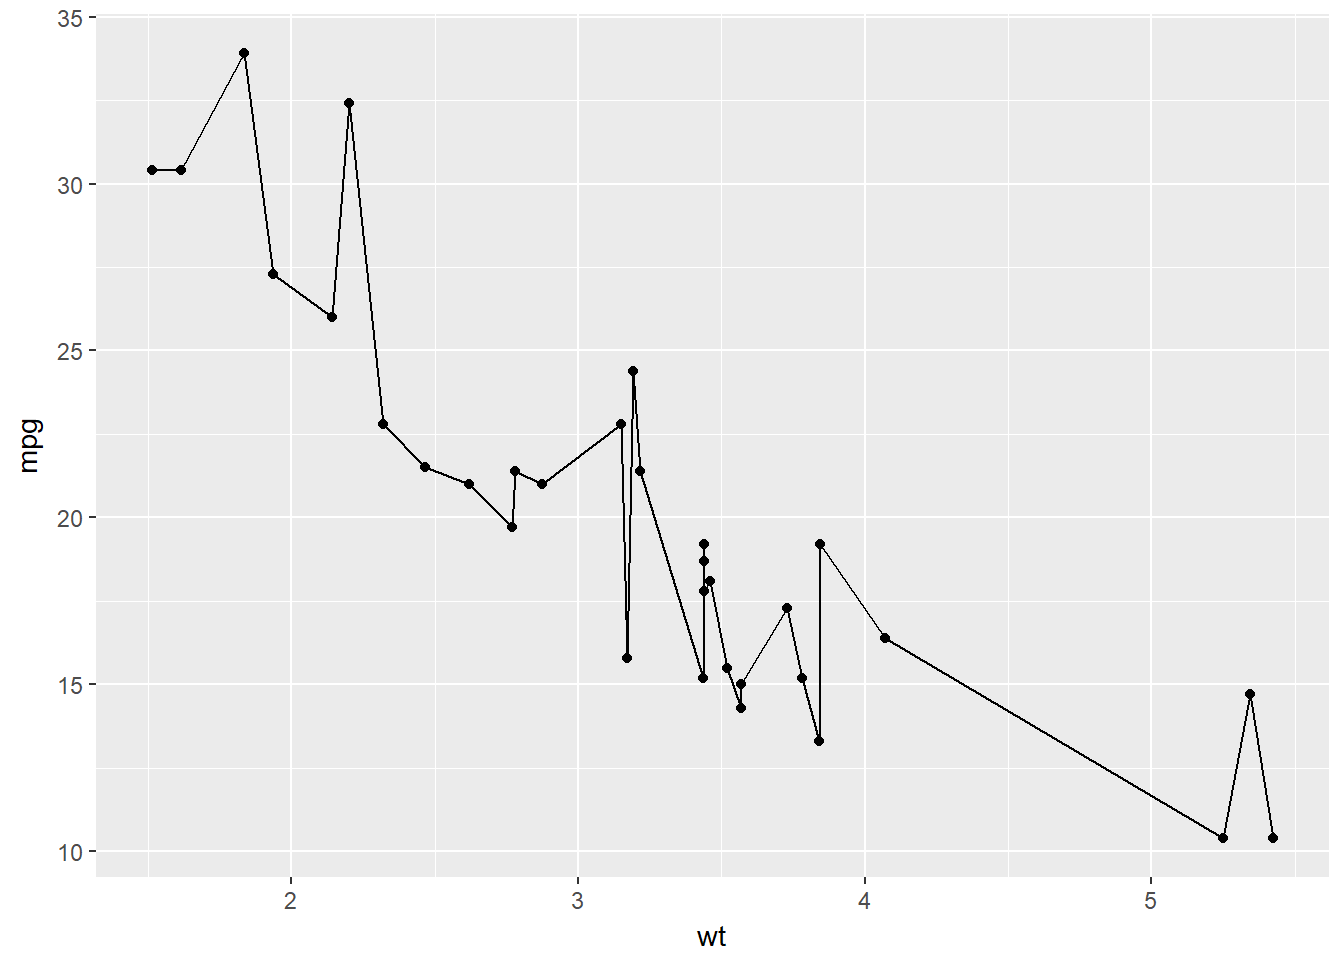
\includegraphics{osnoveR_files/figure-latex/unnamed-chunk-385-1.pdf}

\begin{center}\rule{0.5\linewidth}{\linethickness}\end{center}

Dobili smo što smo tražili, no rezultat nije pretjerano uspješan jer je
linija isprekidana i vizualno ``zakrčuje'' graf umjesto da nam donosi
dodatnu informaciju (inače, linijska geometrija je vrlo popularna kada
radimo sa vremenskim nizovima). Ono što bi nam vjerojatno bilo podesnije
jest ``izglađena'' linija, tj. linija koja aproksimira položaje točaka
koje opisuju težinu i maksimalnu brzinu, umjesto da ih direktno opisuje.
Za ovo su nam potrebni dodatni aspekti koje smo već vidjeli u
inicijalnom pozivu funkcije \texttt{ggplot} (točnije, funkcije
\texttt{layer}) a koje smo u tom trenutku zanemarili, a to su aspekti
statistike i pozicije.

\textbf{Statistika} je aspekt koji provodi neke dodatne izračune nad
podatkovnim skupom prije njegove vizualizacije. To su najčešće izračuni
koje lako možemo i sami provesti ``ručno'', no koje je puno praktičnije
ostaviti na odgovornost vizualizacijskom alatu, pogotovo ako se radi o
izračunu koji se koristi samo za potrebe vizualizacije i nije nam trajno
potreban (npr. stupčasti graf - \emph{bar chart} - prebrojava koliko
puta se pojavljuje koja kategorijska varijabla i to prikazuje visinom
stupca).

Većina statistika provode agregaciju, ali nije pravilo. Neke od češće
korištenih statistika su:

\begin{itemize}
\tightlist
\item
  \texttt{count} - prebrojavanje pojava (za kategorijske varijable)
\item
  \texttt{bin} - raspoređivanje pojava u ladice i prebrojavanje (za
  kontinuirane varijable)
\item
  \texttt{smooth} - ``zaglađivanje'' tj. ``usrednjenje'' korištenjem
  odabrane metode (najčešće \texttt{lm} za linearno ili \texttt{loess}
  za zakrivljeno zaglađivanje)
\item
  \texttt{unique} - uklanjanje duplikata
\item
  \texttt{identity} - direktno preslikavanje, tj. ``ostavljanje kako
  jest''
\end{itemize}

Ovo su samo neke statistike, a dodatne se mogu naći u dokumentaciji.

Svaka statistika ima svoju pomoćnu funkciju koja prati oblik
\texttt{stat\_\textless{}ime\_statistike\textgreater{}} i koja stvara
vlastiti sloj vezan uz tu statistiku.

Vratimo se na naš graf ovisnosti potrošnje o težini automobila, ali ovaj
put umjesto dodavanja sloja linijske geometrije dodajmo sloj koji će
prikazati ``zaglađivanje'' (tj. statistiku \texttt{smooth}). Ovo je
odličan primjer korištenja statističkog aspekta - umjesto da se točke
direktno povežu linijom, uz pomoć posebne funkcije ćemo ``usrednjiti''
vrijednosti a potom ćemo tako usrednjene vrijednosti povezati linijom
ili krivuljom. Za ovo je idealna funkcija \texttt{stat\_smooth} koja će
- ukoliko koristimo default-ne parametre - stvoriti novi sloj sa
``zaglađenim'' prikazom osi \emph{y} u ovisnosti o osi \emph{x},
korištenjem tzv. \texttt{loess} metode, uz prikaz intervala pouzdanosti.
Ovakav sloj možemo lako dodati već prije definiranoj varijabli graf.

\begin{center}\rule{0.5\linewidth}{\linethickness}\end{center}

\textbf{Zadatak 12.9 - funkcija `stat\_smooth' i metoda `lm'}

\begin{Shaded}
\begin{Highlighting}[]
\CommentTok{# dodajte geometriju točaka na varijablu `graf`}
\CommentTok{# te potom dodatni sloj sa krivuljom zaglađivanja}
\CommentTok{# koristite funkciju `stat_smooth` uz parametar `method` }
\CommentTok{# postavljen na `lm` (linearno zaglađivanje)}
\end{Highlighting}
\end{Shaded}

\begin{Shaded}
\begin{Highlighting}[]
\NormalTok{graf }\OperatorTok{+}\StringTok{ }\KeywordTok{geom_point}\NormalTok{() }\OperatorTok{+}\StringTok{ }\KeywordTok{stat_smooth}\NormalTok{(}\DataTypeTok{method =} \StringTok{'lm'}\NormalTok{)}
\end{Highlighting}
\end{Shaded}

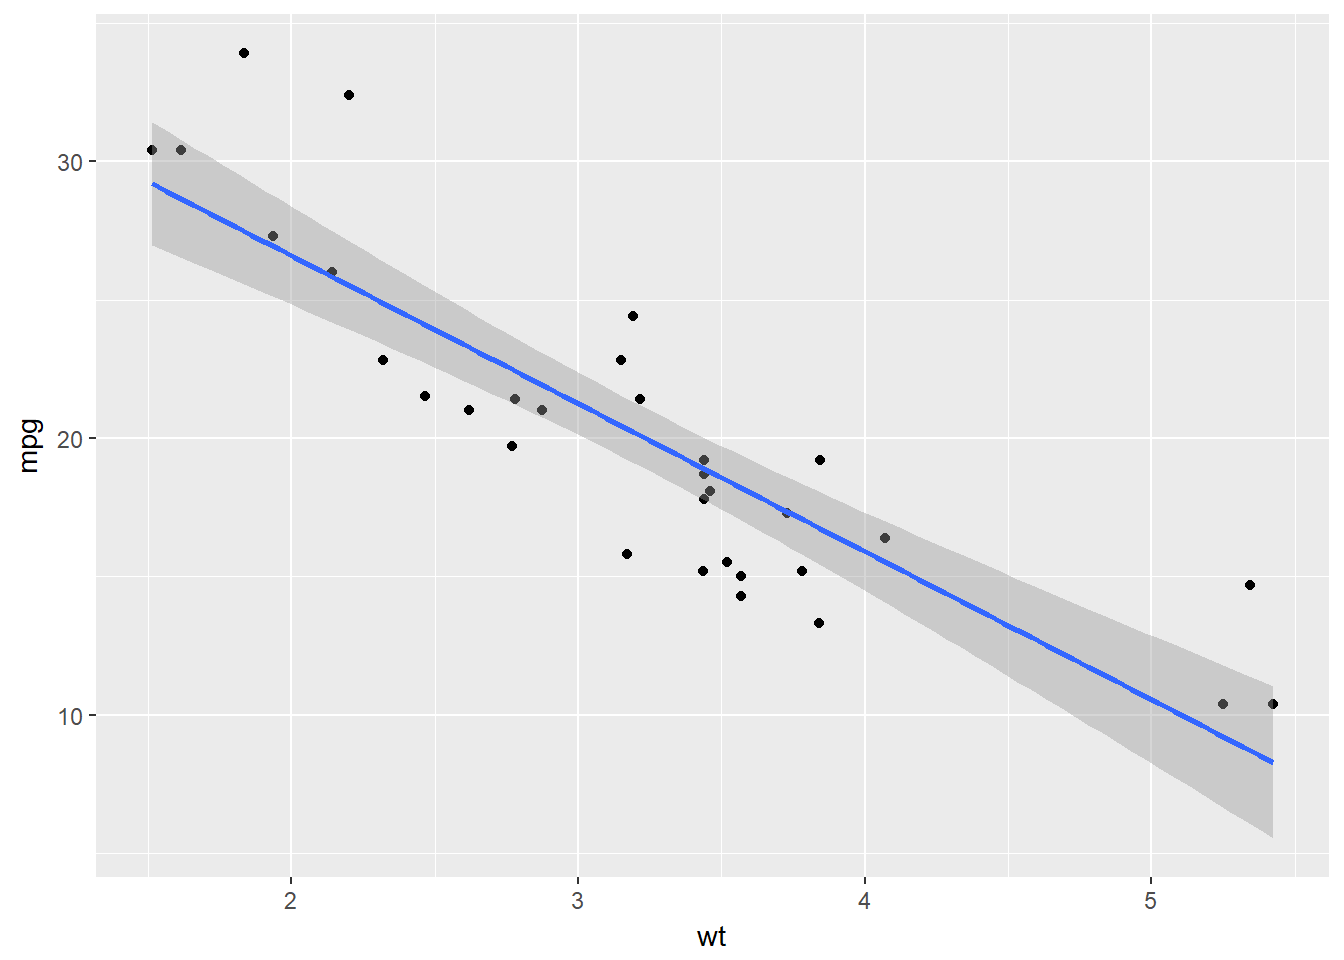
\includegraphics{osnoveR_files/figure-latex/unnamed-chunk-387-1.pdf}

\begin{center}\rule{0.5\linewidth}{\linethickness}\end{center}

\textbf{Zadatak 12.10 - funkcija `stat\_smooth' i metoda `loess'}

\begin{Shaded}
\begin{Highlighting}[]
\CommentTok{# ponovite postupak ali metodu zaglađivanja}
\CommentTok{# postavite na `loess` }
\end{Highlighting}
\end{Shaded}

\begin{Shaded}
\begin{Highlighting}[]
\NormalTok{graf }\OperatorTok{+}\StringTok{ }\KeywordTok{geom_point}\NormalTok{() }\OperatorTok{+}\StringTok{ }\KeywordTok{stat_smooth}\NormalTok{(}\DataTypeTok{method =} \StringTok{'loess'}\NormalTok{)}
\end{Highlighting}
\end{Shaded}

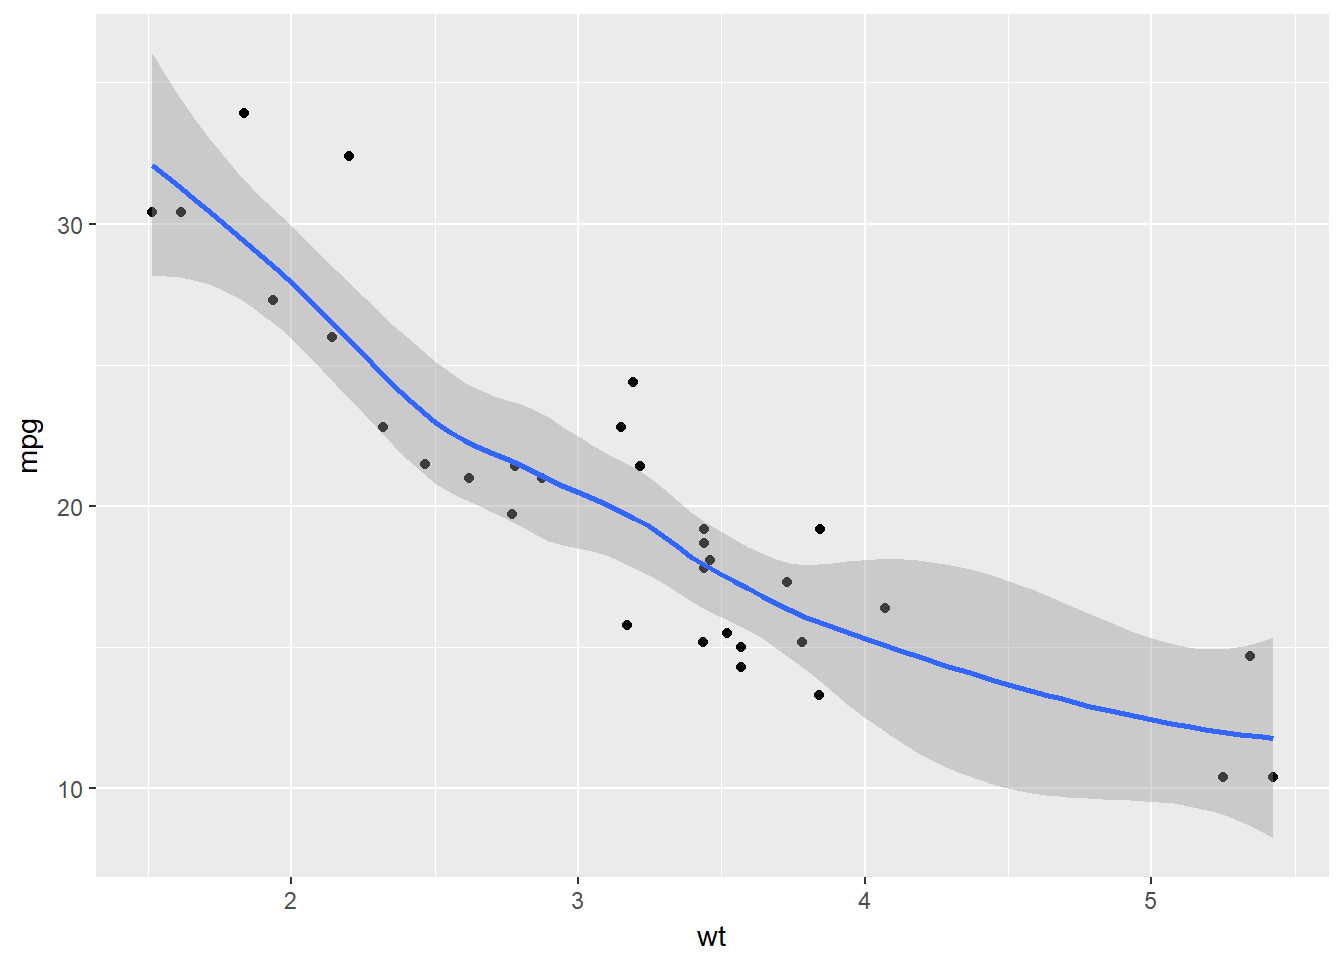
\includegraphics{osnoveR_files/figure-latex/unnamed-chunk-389-1.pdf}

\begin{center}\rule{0.5\linewidth}{\linethickness}\end{center}

\textbf{Zadatak 12.11 - `group' estetika}

\begin{Shaded}
\begin{Highlighting}[]
\CommentTok{# stvorite još jednom isti graf ali sloju zaglađivanja}
\CommentTok{# dodajte estetiku `group` postavljenu na `cyl`}
\CommentTok{# Što smo ovime postigli?}
\end{Highlighting}
\end{Shaded}

\begin{Shaded}
\begin{Highlighting}[]
\NormalTok{graf }\OperatorTok{+}\StringTok{ }\KeywordTok{geom_point}\NormalTok{() }\OperatorTok{+}\StringTok{ }\KeywordTok{stat_smooth}\NormalTok{(}\KeywordTok{aes}\NormalTok{(}\DataTypeTok{group =}\NormalTok{ cyl), }\DataTypeTok{method =} \StringTok{'loess'}\NormalTok{)}
\end{Highlighting}
\end{Shaded}

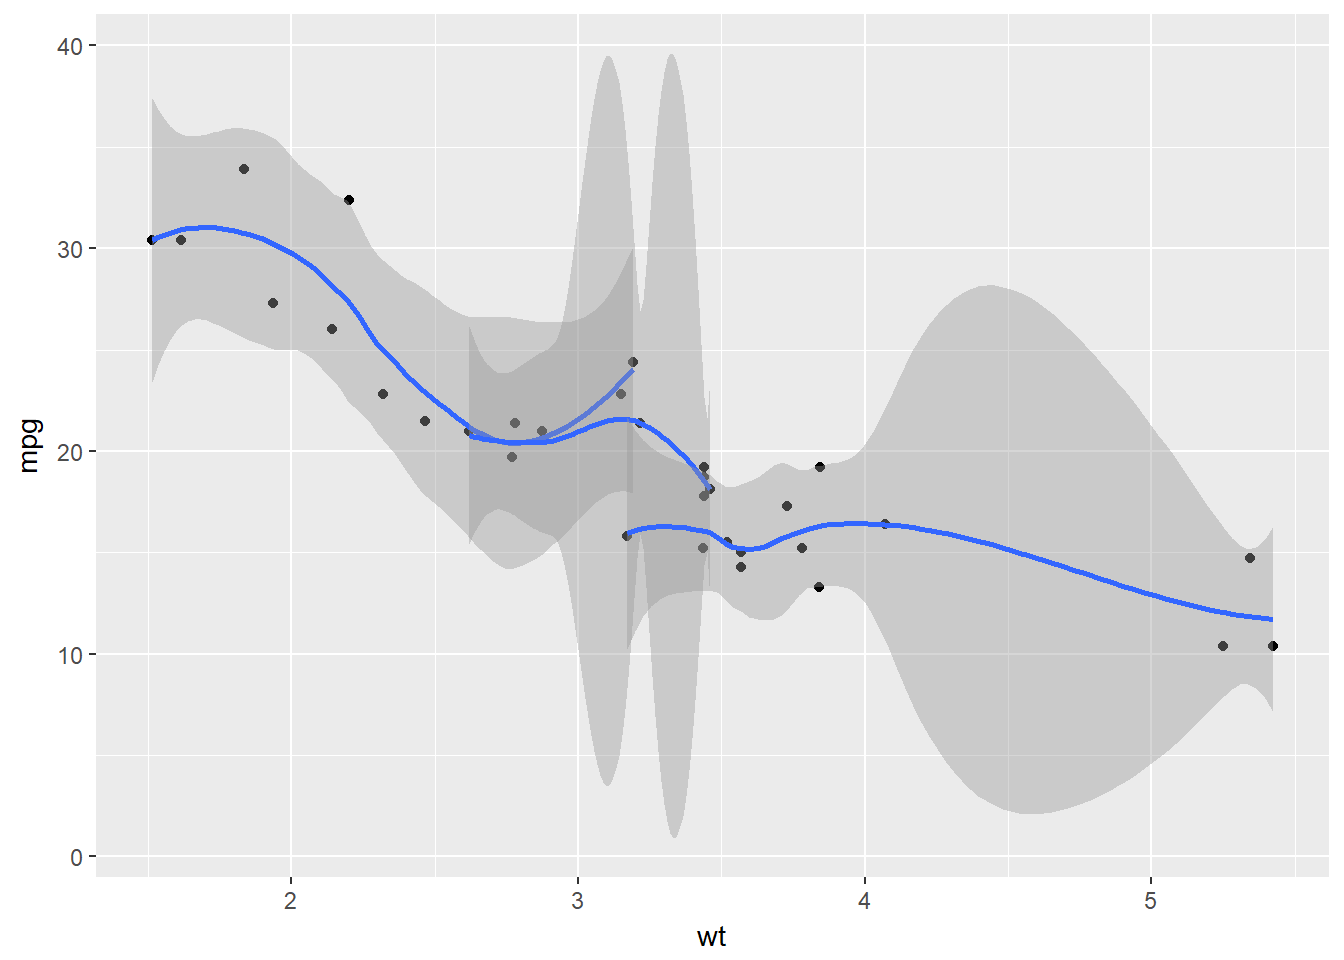
\includegraphics{osnoveR_files/figure-latex/unnamed-chunk-391-1.pdf}

\begin{center}\rule{0.5\linewidth}{\linethickness}\end{center}

U zadnjem primjeru vidjeli smo tzv. \texttt{group} estetiku. Ona radi
slično \emph{group\_by} funkciji iz SQL-a ili \texttt{dplyr}-a, tj. ako
računamo agregacije nad nekim skupom podataka, onda se umjesto nad
cijelim podatkovnim skupom one rade nad svakom definiranom grupom
zasebno. Korištenjem ove estetike možemo na grafu prikazati zasebne
izračune prema odabranoj grupi, pa tako je i u ovom primjeru
zaglađivanje rađeno po ``podgrupama'' ovisno o broju cilindara.

Kod nekih vizualizacija može se dogoditi da su podaci već ``grupirani''
ali mi želimo dodati geometriju koja radi nad cijelim podatkovnim skupom
- u tom slučaju najlakše je jednostavno postaviti \texttt{group}
estetiku na brojku \texttt{1}, što će R interpretirati kao ``sve je
jedna grupa'' te to tako i prikazati.

\begin{center}\rule{0.5\linewidth}{\linethickness}\end{center}

\subsection{Povezanost geometrije i
statistike}\label{povezanost-geometrije-i-statistike}

U pravilu određene geometrije prirodno koriste ``svoje'' statistike
(npr. stupčasti graf nastaje tako što se prebrojavaju pojave određene
kategorije što se onda reprezentira visinom stupca). U praksi ovo znači
da kod vizualizacije ``statističkih'' slojeva zapravo imamo mogućnost
definiranja \texttt{geom} sloja sa \texttt{stat} parametrom ili
\texttt{stat} sloja sa \texttt{geom} parametrom - pri čemu često nije
potrebno ni posebno podešavati ``prateći'' parametar budući da je po
\emph{default}-u postavljen na onaj koji nam treba. Tako npr.
\texttt{geom\_bar} već unaprijed koristi \texttt{count} statistiku, a
ponaša se analogno \texttt{stat\_count} funkciji koja već ima
postavljenu \texttt{bar} geometriju.

Koju onda pomoćnu funkciju izabrati, \texttt{stat} ili \texttt{geom}?
Ovo je zapravo potpuno nebitno, budući da je učinak isti, ali u praksi
se nešto češće koriste \texttt{geom} funkcije većinom zbog malo
konzistentnije sintakse izgradnje grafa.

Pokušajmo sada napraviti stupčani graf (engl. \emph{bar plot}) koji će
visinom stupića prikazati broj pojavljivanja određene kategorije - npr.
zastupljenost pojedinog broja cilindara u okviru \texttt{mtcars}. Za ovo
koristimo pomoćnu funkciju \texttt{geom\_bar} koja ima unaprijed
postavljenu \texttt{count} statistiku.

\begin{center}\rule{0.5\linewidth}{\linethickness}\end{center}

\textbf{Zadatak 12.12 - stupčasti graf}

\begin{Shaded}
\begin{Highlighting}[]
\CommentTok{# nacrtajte stupčani graf varijable `cyl` tablice `mtcars` }
\CommentTok{# koristite funkciju `geom_bar` ili `stat_count`}
\end{Highlighting}
\end{Shaded}

\begin{Shaded}
\begin{Highlighting}[]
\KeywordTok{ggplot}\NormalTok{(mtcars, }\KeywordTok{aes}\NormalTok{(}\DataTypeTok{x =}\NormalTok{ cyl)) }\OperatorTok{+}\StringTok{ }\KeywordTok{geom_bar}\NormalTok{()}
\end{Highlighting}
\end{Shaded}

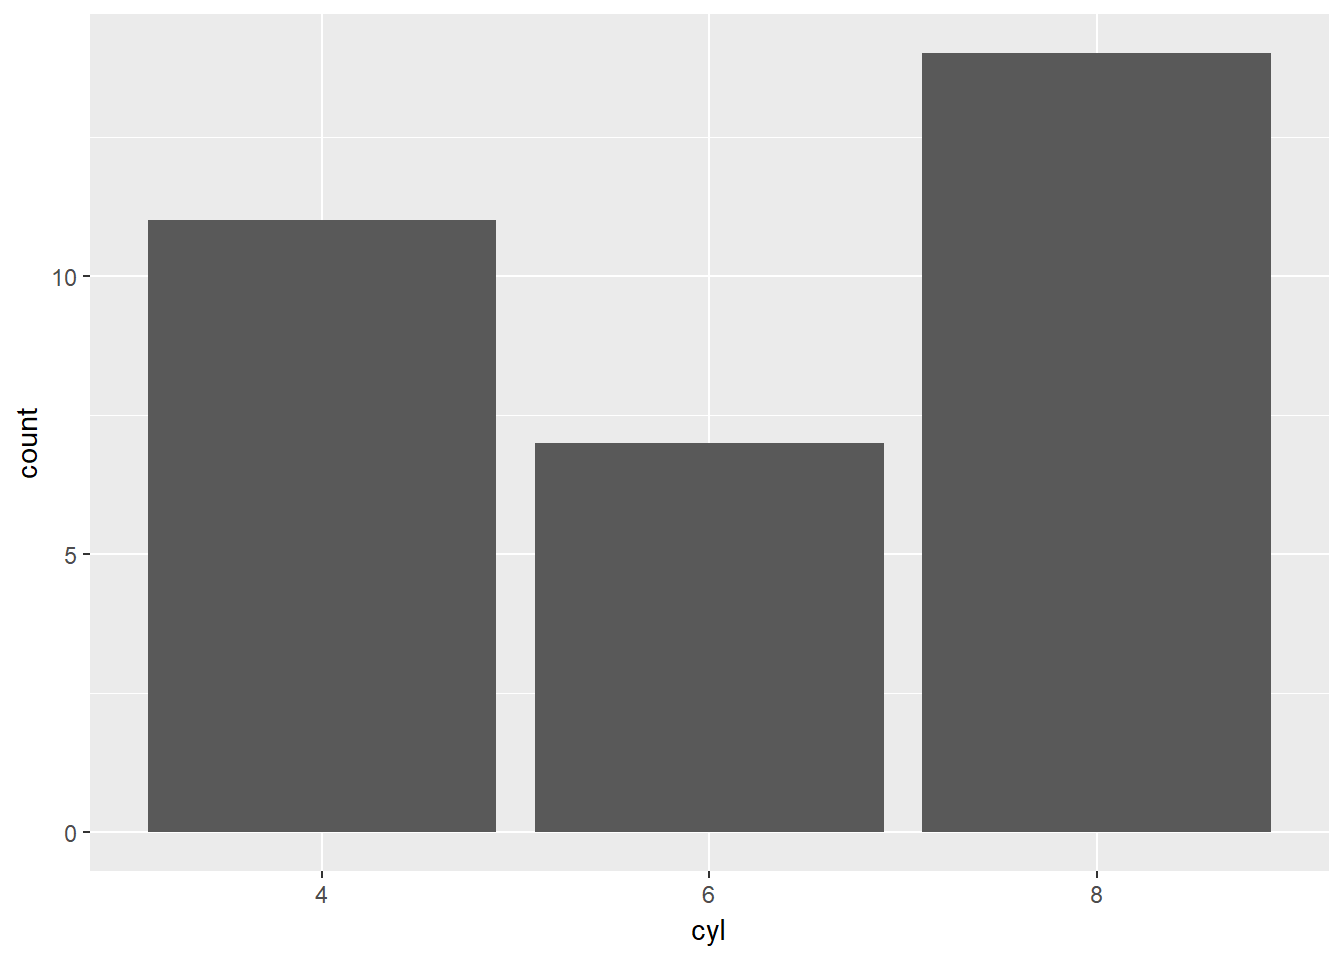
\includegraphics{osnoveR_files/figure-latex/unnamed-chunk-393-1.pdf}

\begin{center}\rule{0.5\linewidth}{\linethickness}\end{center}

Na sličan način možemo prikazati i kontinuirane varijable. Za razliku od
stupčanog grafa, gdje imamo jasno definirane kategorije, ovdje ćemo
morati prvo grupirati vrijednosti u tzv. ``ladice'' (engl. \emph{bins})
na osnovu kojih gradimo graf koji se zove \emph{histogram}. Opet
koristimo statistiku \texttt{bin}, a za samo stvaranje histograma
koristit ćemo pomoćnu funkciju \texttt{geom\_histogram}.

\begin{center}\rule{0.5\linewidth}{\linethickness}\end{center}

\textbf{Zadatak 12.13 - histogram}

\begin{Shaded}
\begin{Highlighting}[]
\CommentTok{# nacrtajte histogram varijable `wt` tablice `mtcars`}
\CommentTok{# težine podijelite jednoliko u četiri ladice}
\CommentTok{# koristite funkciju `geom_histogram`}
\end{Highlighting}
\end{Shaded}

\begin{Shaded}
\begin{Highlighting}[]
\KeywordTok{ggplot}\NormalTok{(mtcars, }\KeywordTok{aes}\NormalTok{(}\DataTypeTok{x =}\NormalTok{ wt)) }\OperatorTok{+}\StringTok{ }\KeywordTok{geom_histogram}\NormalTok{(}\DataTypeTok{bins =} \DecValTok{4}\NormalTok{)}
\end{Highlighting}
\end{Shaded}

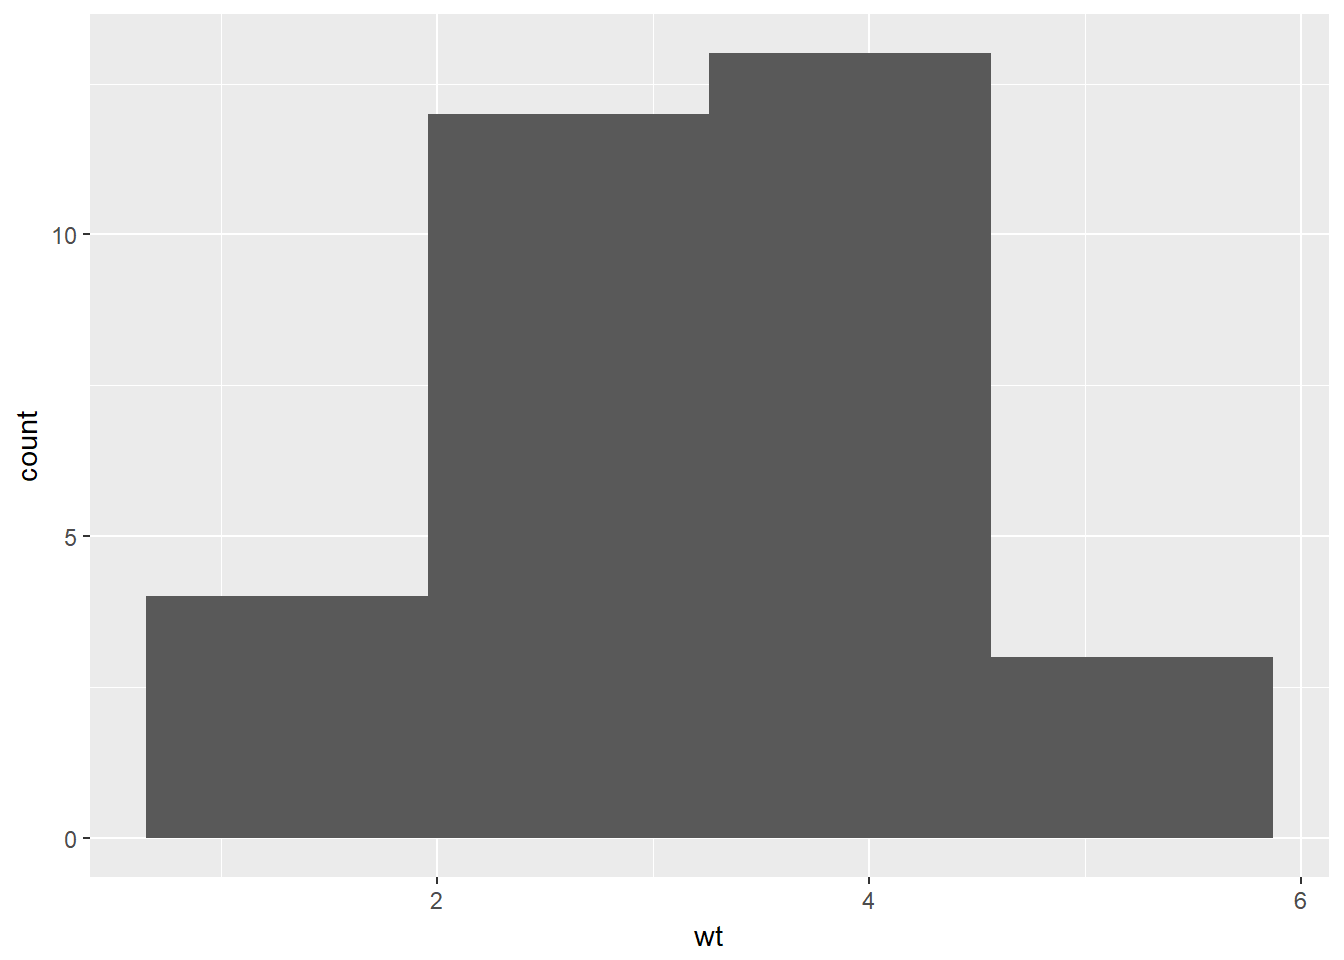
\includegraphics{osnoveR_files/figure-latex/unnamed-chunk-395-1.pdf}

\begin{center}\rule{0.5\linewidth}{\linethickness}\end{center}

Kako zapravo radi statistički aspekt? U pravilu se na osnovu postojećih
varijabli izračunavaju jedna ili više novih, najčešće agregiranih
varijabli. U dokumentaciji možemo naći konkretne informacije o nazivima
tih novih varijabli i njihovom značenju. Na primjer, ako pogledamo
dokumentaciju za funkciju \texttt{stat\_bin}, možemo vidjeti da ona
stvara varijable imena \texttt{count}, \texttt{ncount}, \texttt{density}
i \texttt{ndensity}. Bilo koja od ovih varijabli može se koristiti kao
``visina stupića'', tj. kao estetika \emph{y}. Razlog zašto ovu estetiku
nismo eksplicitno navodili u prethodnom primjeru jest činjenica da
funkcija statistike automatski odabire onu agregatnu funkciju koja se
očekivano najčešće koristi (u našem slučaju je to bila \texttt{count}).
Ukoliko želimo obaviti neku drugu agregaciju, možemo i eksplicitno
postaviti estetiku y na odabranu varijablu, samo moramo koristiti
\texttt{ggplot2} konvenciju gdje takvim varijablama kao prefiks i sufiks
postavljamo \texttt{..}, kao npr:

\begin{Shaded}
\begin{Highlighting}[]
\KeywordTok{aes}\NormalTok{(}\DataTypeTok{x =}\NormalTok{ hp, }\DataTypeTok{y =}\NormalTok{ ..density..)}
\end{Highlighting}
\end{Shaded}

Pokušajmo ovo isprobati na primjeru.

\textbf{Zadatak 12.14 - histogram / `ncount'}

\begin{Shaded}
\begin{Highlighting}[]
\CommentTok{# nacrtajte histogram varijable `wt` tablice `mtcars`}
\CommentTok{# težine podijelite jednoliko u četiri ladice}
\CommentTok{# koristite funkciju `geom_histogram`}
\CommentTok{# za agregacijsku varijablu postavite `ncount` }
\CommentTok{# prokomentirajte dobiveni rezultat}
\end{Highlighting}
\end{Shaded}

\begin{Shaded}
\begin{Highlighting}[]
\KeywordTok{ggplot}\NormalTok{(mtcars, }\KeywordTok{aes}\NormalTok{(}\DataTypeTok{x =}\NormalTok{ wt, }\DataTypeTok{y =}\NormalTok{ ..ncount..)) }\OperatorTok{+}\StringTok{ }\KeywordTok{geom_histogram}\NormalTok{(}\DataTypeTok{bins =} \DecValTok{4}\NormalTok{)}
\end{Highlighting}
\end{Shaded}

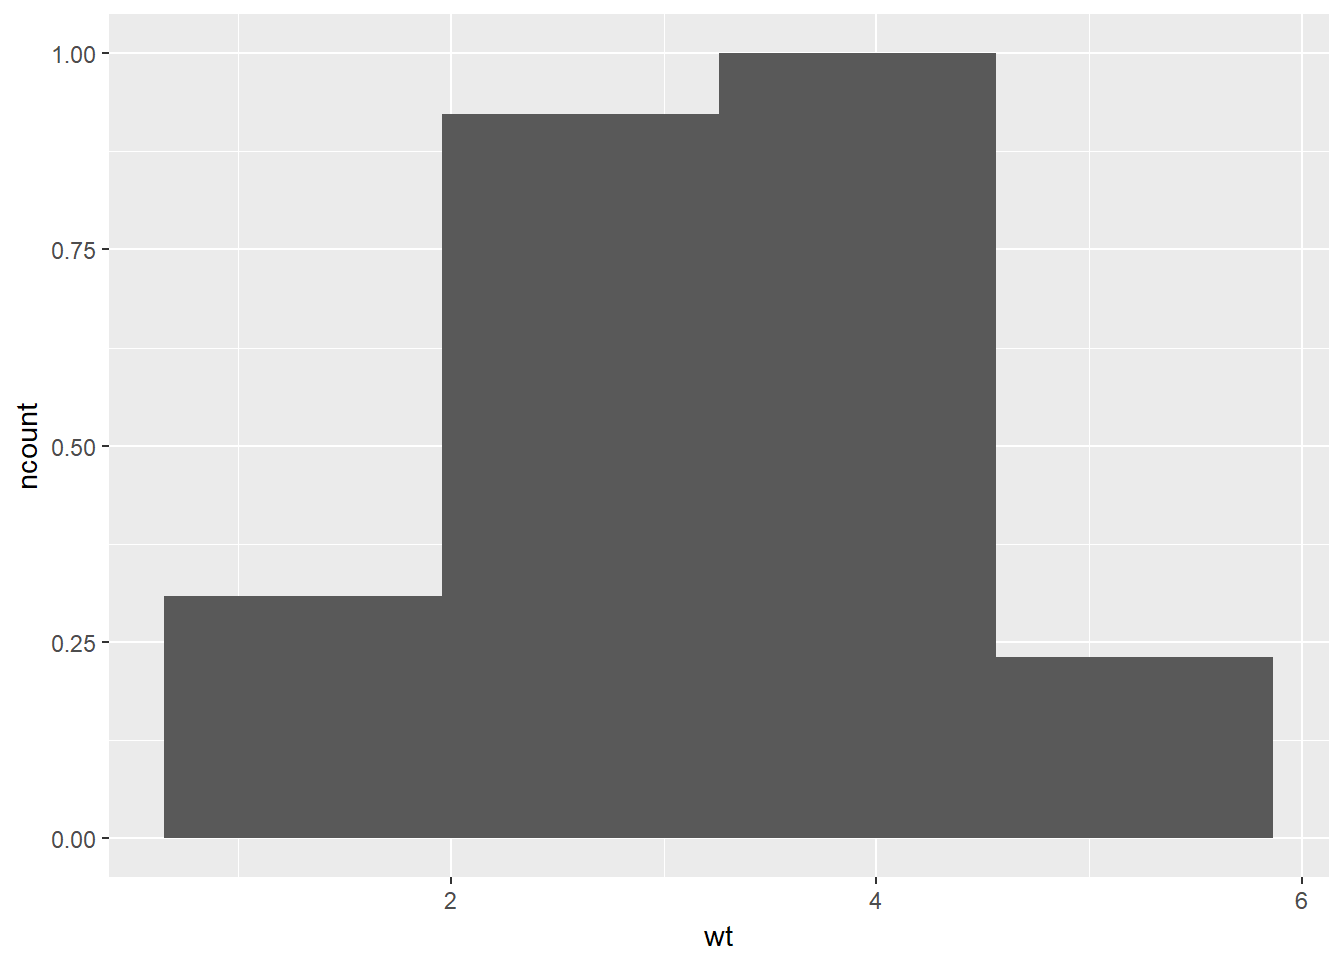
\includegraphics{osnoveR_files/figure-latex/unnamed-chunk-398-1.pdf}

\begin{center}\rule{0.5\linewidth}{\linethickness}\end{center}

Otiđimo sada korak dalje. Nacrtajte isti histogram (sa
\emph{default}-nom \texttt{count} agregacijom), no prikažite na njemu i
koliko je unutar svake kategorije zastupljen koji broj cilindara. Ovo
ćete lako izvesti dodavanjem estetike \texttt{fill} koja reprezentira
``punjenje'' stupića bojom (za razliku od estetike \texttt{color} koja
bi u slučaju stupčanog grafa bojala linije oko pravokutnika).

\begin{center}\rule{0.5\linewidth}{\linethickness}\end{center}

\textbf{Zadatak 12.15 - `fill' estetika u histogramu}

\begin{Shaded}
\begin{Highlighting}[]
\CommentTok{# nacrtajte histogram varijable `wt`, uz dodanu varijablu `cyl` na estetici `fill`}
\end{Highlighting}
\end{Shaded}

\begin{Shaded}
\begin{Highlighting}[]
\KeywordTok{ggplot}\NormalTok{(mtcars, }\KeywordTok{aes}\NormalTok{(}\DataTypeTok{x =}\NormalTok{ wt, }\DataTypeTok{fill =}\NormalTok{ cyl)) }\OperatorTok{+}\StringTok{ }\KeywordTok{geom_histogram}\NormalTok{(}\DataTypeTok{bins =} \DecValTok{4}\NormalTok{)}
\end{Highlighting}
\end{Shaded}

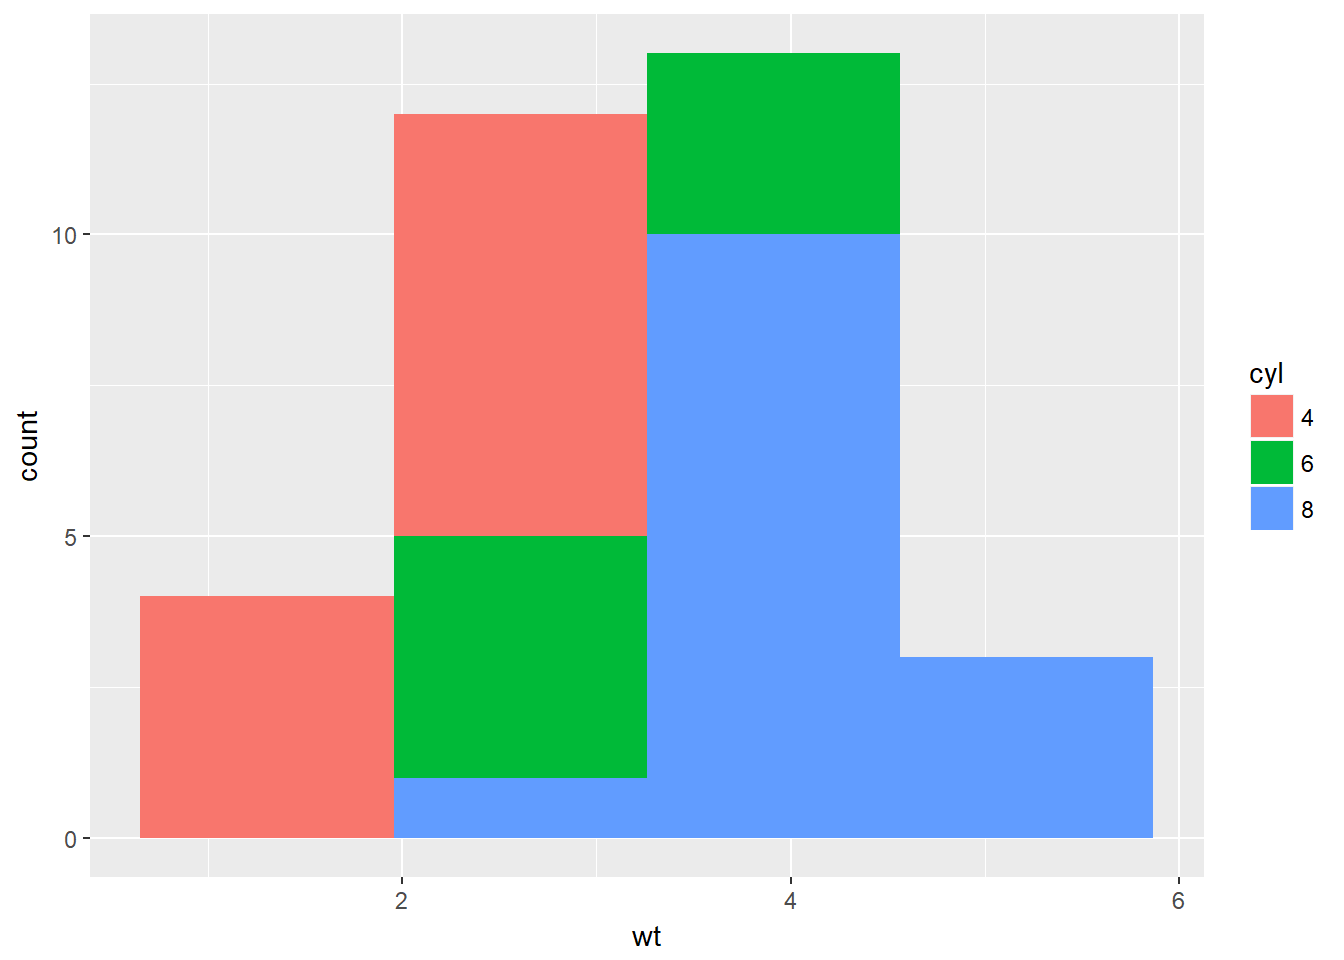
\includegraphics{osnoveR_files/figure-latex/unnamed-chunk-400-1.pdf}

\begin{center}\rule{0.5\linewidth}{\linethickness}\end{center}

Ovdje vidimo primjer ``kombiniranog'' histograma - funkcija će zapravo
izračunati frekvencije pojavljivanja za svaku kategoriju težine te za
svaki broj cilindara. Jedan od načina kako ovo prikazati bio bi
trodimenzionalni graf gdje bi u baznoj ravnini bile kombinacije dvije
navedene varijable dok bi treća dimenzija bila rezervirana za visinu
stupića - no kod projekcije takvog grafa na dvodimenzionalnu ravninu
stupići bi se međusobno prekrivali. Kako bi se rezultati mogli
učinkovito prikazati na dvodimenzionalnom grafu, stupići su
``repozicionirani'' tako da su je stupić za pojedine cilindre postavljen
jedan na drugi u sklopu iste kategorije težine. Ovo je zapravo primjer
korištenja tzv. \emph{pozicijskog aspekta} ili jednostavno
\emph{pozicije}.

\textbf{Pozicija} je aspekt koji omogućuje ``razmještanje'' određenog
aspekta grafa ukoliko je to potrebno zbog jasnoće prikaza. U prethodnom
primjeru već smo uočili ``raslojavanje'' stupića prema kategorijskoj
varijabli. U ovom slučaju funkcija je zapravo koristila pozicijski
aspekt \texttt{"stack"} koji ``male'' stupiće razmješta tako da ih slaže
jedan na drugi. Alternativa je postavljanje aspekta pozicije
(\texttt{position}) na ``izbjegavanje'' - \texttt{"dodge"}- kod kojeg će
stupići biti nacrtani u grupicama jedan pored drugog.

\begin{center}\rule{0.5\linewidth}{\linethickness}\end{center}

\textbf{Zadatak 12.16 - pozicijski aspekt `dodge'}

\begin{Shaded}
\begin{Highlighting}[]
\CommentTok{# nacrtajte isti histogram, ali pozicijski aspekt `position` postavite na `"dodge"`}
\end{Highlighting}
\end{Shaded}

\begin{Shaded}
\begin{Highlighting}[]
\KeywordTok{ggplot}\NormalTok{(mtcars, }\KeywordTok{aes}\NormalTok{(}\DataTypeTok{x =}\NormalTok{ wt, }\DataTypeTok{fill =}\NormalTok{ cyl)) }\OperatorTok{+}\StringTok{ }\KeywordTok{geom_histogram}\NormalTok{(}\DataTypeTok{bins =} \DecValTok{4}\NormalTok{, }\DataTypeTok{position =} \StringTok{"dodge"}\NormalTok{)}
\end{Highlighting}
\end{Shaded}

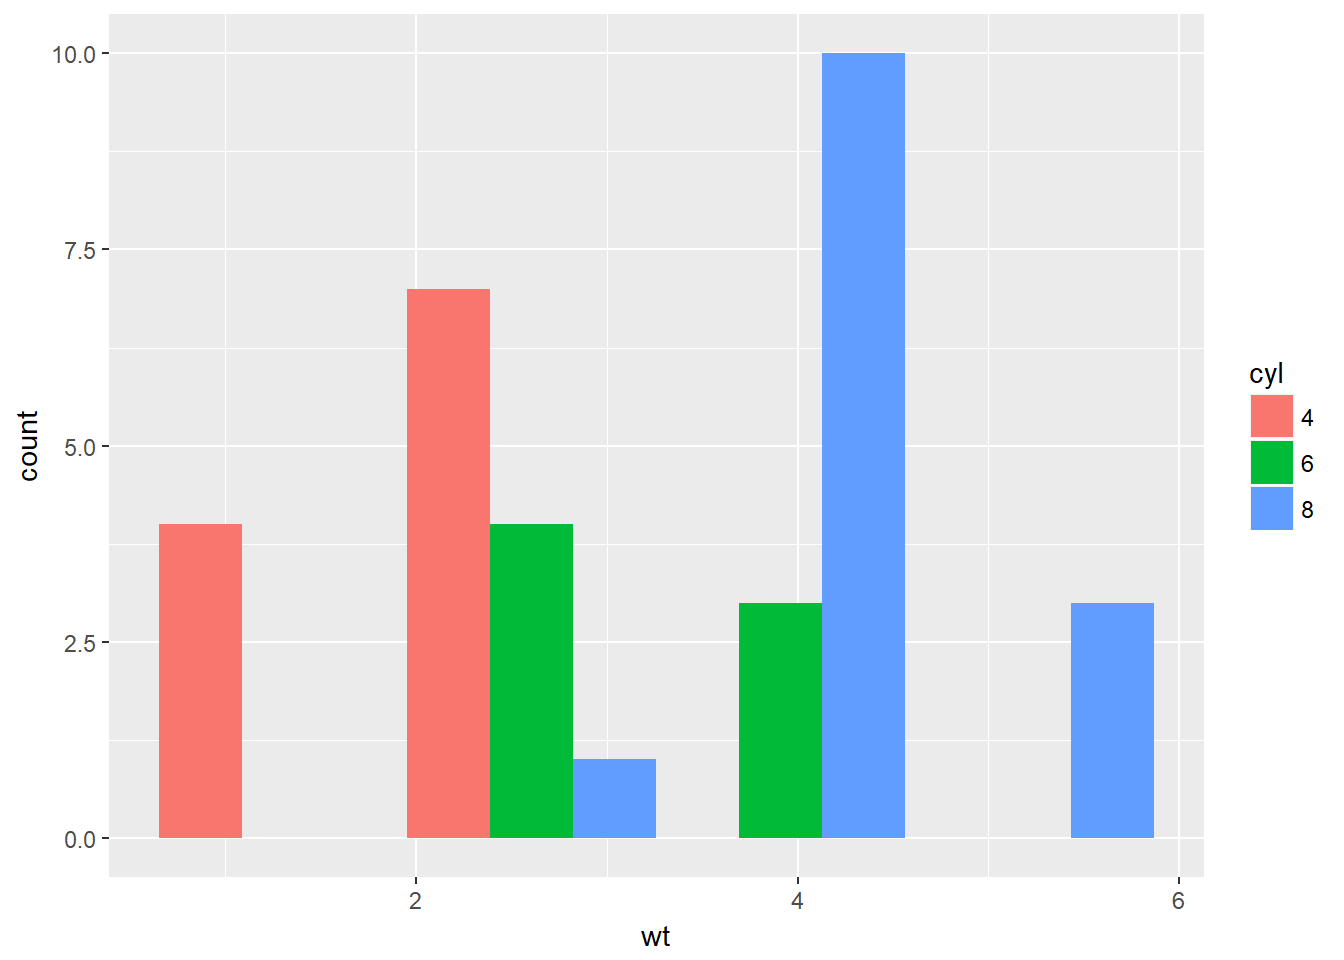
\includegraphics{osnoveR_files/figure-latex/unnamed-chunk-402-1.pdf}

\begin{center}\rule{0.5\linewidth}{\linethickness}\end{center}

Uočite da smo korištenjem ``izbjegavanja'' izgubili precizan prikaz
intervala pojedine ladice, ali smo dobili jasniji prikaz odnosa između
zastupljenosti pojedinih kategorija unutar pojedine ladice.

\begin{center}\rule{0.5\linewidth}{\linethickness}\end{center}

\textbf{Zadatak 12.17 - pozicijski aspekt `identity'}

\begin{Shaded}
\begin{Highlighting}[]
\CommentTok{# nacrtajte opet isti histogram, ali pozicijski aspekt }
\CommentTok{# `position` postavite na `"identity"`}
\CommentTok{# parametar geometrije `alpha` postavite na 0.2 }
\end{Highlighting}
\end{Shaded}

\begin{Shaded}
\begin{Highlighting}[]
\KeywordTok{ggplot}\NormalTok{(mtcars, }\KeywordTok{aes}\NormalTok{(}\DataTypeTok{x =}\NormalTok{ wt, }\DataTypeTok{fill =}\NormalTok{ cyl)) }\OperatorTok{+}\StringTok{ }
\StringTok{  }\KeywordTok{geom_histogram}\NormalTok{(}\DataTypeTok{bins =} \DecValTok{4}\NormalTok{, }\DataTypeTok{position =} \StringTok{"identity"}\NormalTok{, }\DataTypeTok{alpha =} \FloatTok{0.4}\NormalTok{)}
\end{Highlighting}
\end{Shaded}

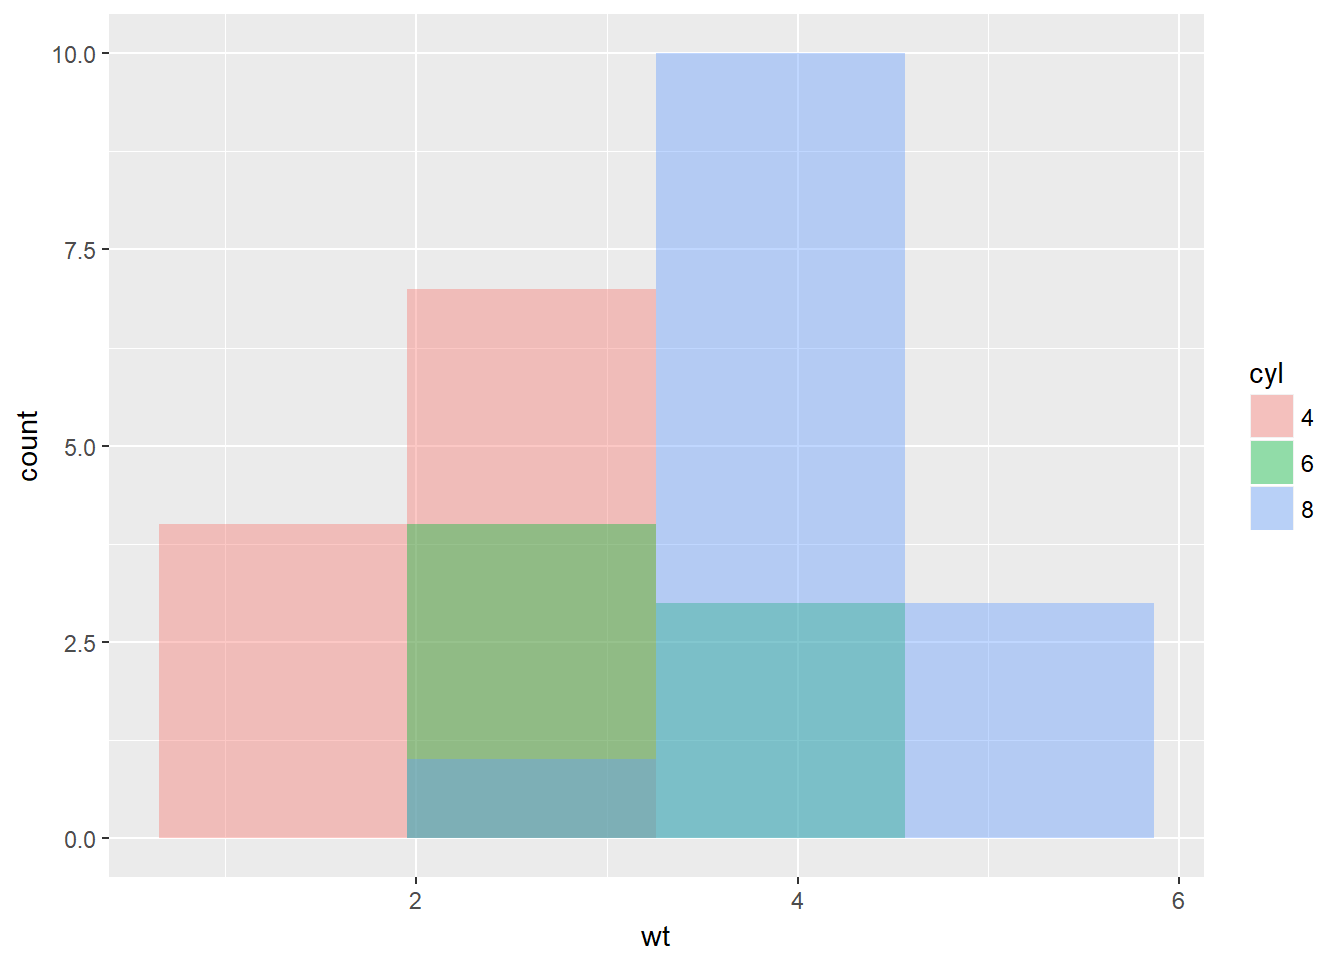
\includegraphics{osnoveR_files/figure-latex/unnamed-chunk-404-1.pdf}

\begin{center}\rule{0.5\linewidth}{\linethickness}\end{center}

Kao što vidimo, pozicijski aspekt \texttt{"identity"} znači ``bez
repozicioniranja''.

Pokažimo još jedan pozicijski aspekt - \texttt{"fill"} (nemojte ga
miješati sa estetikom \texttt{fill}!).

\begin{center}\rule{0.5\linewidth}{\linethickness}\end{center}

\textbf{Zadatak 12.18 - pozicijski aspekt `fill'}

\begin{Shaded}
\begin{Highlighting}[]
\CommentTok{# nacrtajte isti histogram, ali uz pozicijski aspekt postavljen na `fill`}
\CommentTok{# radi bolje vidljivosti pravokutnike uokvirite crnom linijom}
\CommentTok{# objasnite rezultat. Što smo postigli ovakvim histogramom?}
\end{Highlighting}
\end{Shaded}

\begin{Shaded}
\begin{Highlighting}[]
\KeywordTok{ggplot}\NormalTok{(mtcars, }\KeywordTok{aes}\NormalTok{(}\DataTypeTok{x =}\NormalTok{ wt, }\DataTypeTok{fill =}\NormalTok{ cyl)) }\OperatorTok{+}\StringTok{ }
\StringTok{  }\KeywordTok{geom_histogram}\NormalTok{(}\DataTypeTok{bins =} \DecValTok{4}\NormalTok{, }\DataTypeTok{color =} \StringTok{"Black"}\NormalTok{, }\DataTypeTok{position =} \StringTok{"fill"}\NormalTok{)}
\end{Highlighting}
\end{Shaded}

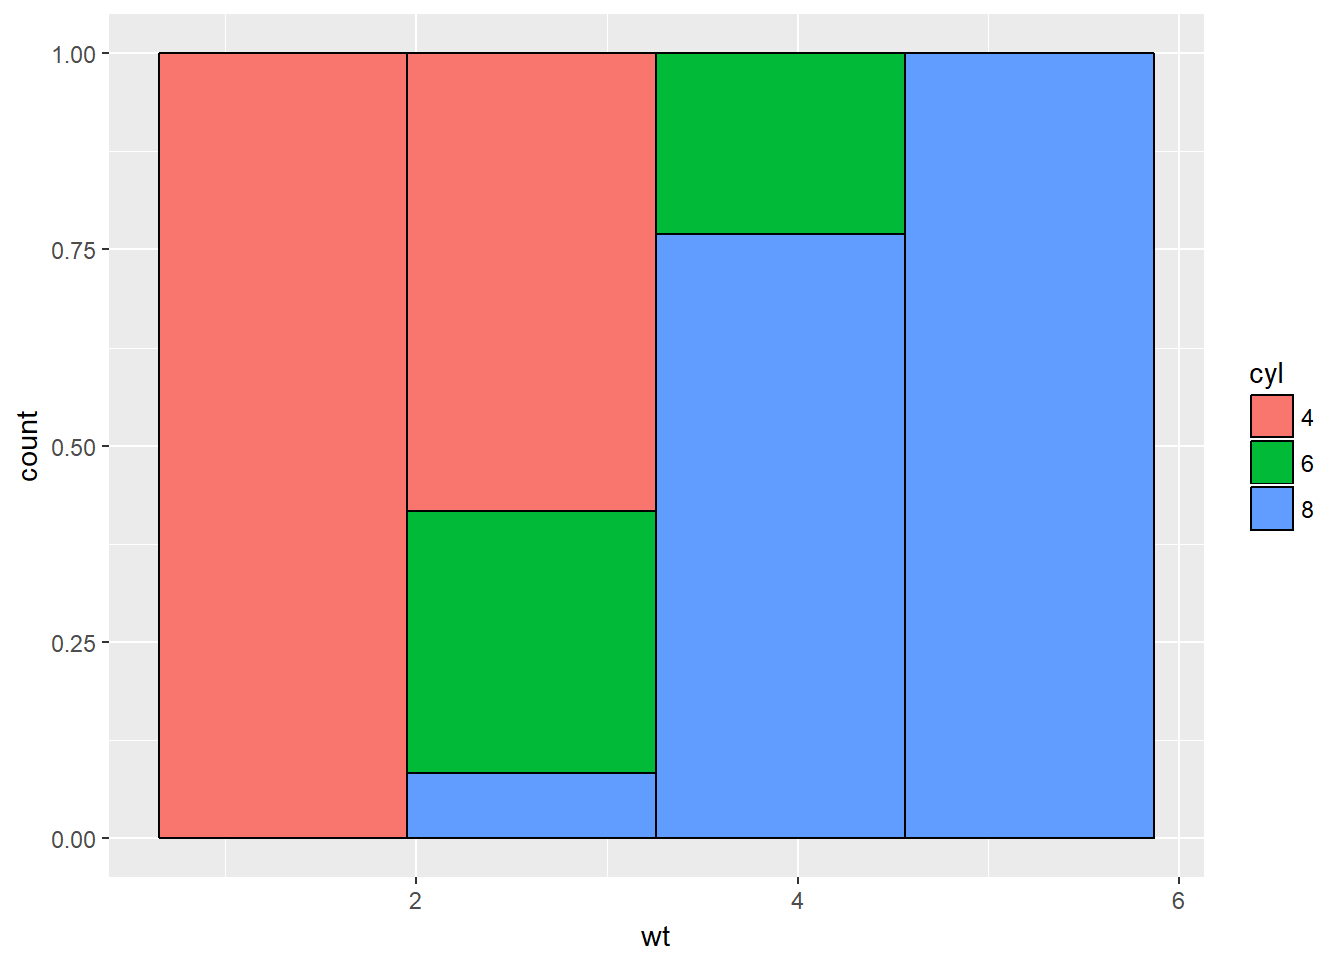
\includegraphics{osnoveR_files/figure-latex/unnamed-chunk-406-1.pdf}

\begin{center}\rule{0.5\linewidth}{\linethickness}\end{center}

Konačni primjer pozicijskog aspekta kojeg ćemo prikazati je dodavanje
``šuma'' obzervacijama koje prikazujemo točkastim grafom a koje
prekrivaju jedna drugu te djeluju kao jedna obzervacija. Dodavanjem
pozicijskog aspekta \texttt{jitter} možemo bolje vizualno komunicirati
da se radi o većem broju obzervacija (ovo je učinkovito za manje
podatkovne skupove, za veće ćemo često bolje rezultate postići
korištenjem parametra transparentnosti, smanjivanjem veličine točaka ili
uzorkovanjem skupa prije vizualizacije).

Za primjer ćemo stvoriti jedan ``umjetni'' podatkovni okvir od 100
``prekrivajućih'' obzervacija.

\begin{center}\rule{0.5\linewidth}{\linethickness}\end{center}

\textbf{Zadatak 12.19 - pozicijski aspekt `jitter'}

\begin{Shaded}
\begin{Highlighting}[]
\NormalTok{df <-}\StringTok{ }\KeywordTok{data.frame}\NormalTok{( }\DataTypeTok{x =} \KeywordTok{c}\NormalTok{(}\KeywordTok{rep}\NormalTok{(}\DecValTok{1}\NormalTok{, }\DecValTok{90}\NormalTok{), }\KeywordTok{rep}\NormalTok{(}\DecValTok{2}\NormalTok{, }\DecValTok{9}\NormalTok{), }\DecValTok{3}\NormalTok{),}
                  \DataTypeTok{y =} \KeywordTok{c}\NormalTok{(}\KeywordTok{rep}\NormalTok{(}\DecValTok{1}\NormalTok{, }\DecValTok{70}\NormalTok{), }\KeywordTok{rep}\NormalTok{(}\DecValTok{2}\NormalTok{, }\DecValTok{25}\NormalTok{), }\KeywordTok{rep}\NormalTok{(}\DecValTok{3}\NormalTok{, }\DecValTok{5}\NormalTok{)))}
\CommentTok{# prikažite navedeni okvir uz pomoć `scatterplot` grafa, tj. točkaste geometrije}
\end{Highlighting}
\end{Shaded}

\begin{Shaded}
\begin{Highlighting}[]
\KeywordTok{ggplot}\NormalTok{(df, }\KeywordTok{aes}\NormalTok{(}\DataTypeTok{x =}\NormalTok{ x, }\DataTypeTok{y =}\NormalTok{ y)) }\OperatorTok{+}\StringTok{ }\KeywordTok{geom_point}\NormalTok{()}
\end{Highlighting}
\end{Shaded}

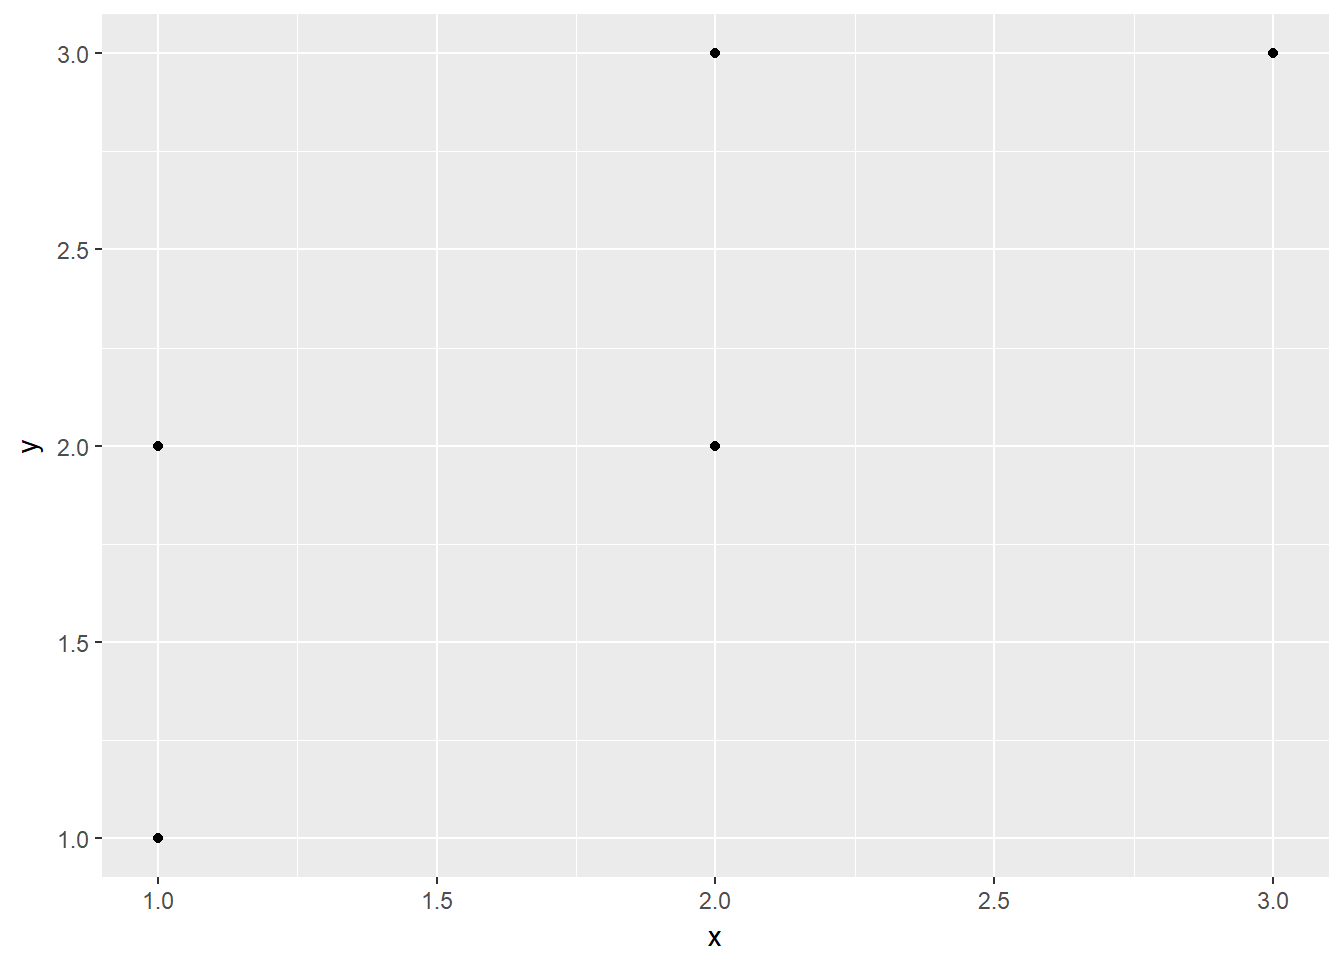
\includegraphics{osnoveR_files/figure-latex/unnamed-chunk-408-1.pdf}

\begin{center}\rule{0.5\linewidth}{\linethickness}\end{center}

\textbf{Zadatak 12.20 - pozicijski aspekt `jitter' (2)}

\begin{Shaded}
\begin{Highlighting}[]
\CommentTok{# prikažite isti graf, ali umjesto `geom_point` upotrijebite}
\CommentTok{# pomoćnu funkciju `geom_jitter` koja ima ugrađen `jitter` pozicijski aspekt}
\CommentTok{# postavite `width` i `height` parametre na 0.3 (30% dodanog šuma)}
\CommentTok{# dodatno postavite `color` parametar geometrije na "blue" }
\CommentTok{# i `alpha` parametar ("prozirnost") na 0.4 }
\end{Highlighting}
\end{Shaded}

\begin{Shaded}
\begin{Highlighting}[]
\KeywordTok{ggplot}\NormalTok{(df, }\KeywordTok{aes}\NormalTok{(}\DataTypeTok{x =}\NormalTok{ x, }\DataTypeTok{y =}\NormalTok{ y)) }\OperatorTok{+}\StringTok{ }
\StringTok{  }\KeywordTok{geom_jitter}\NormalTok{(}\DataTypeTok{width =} \FloatTok{0.3}\NormalTok{, }\DataTypeTok{height =} \FloatTok{0.3}\NormalTok{, }\DataTypeTok{alpha =} \FloatTok{0.4}\NormalTok{, }\DataTypeTok{color =} \StringTok{"blue"}\NormalTok{)}
\end{Highlighting}
\end{Shaded}

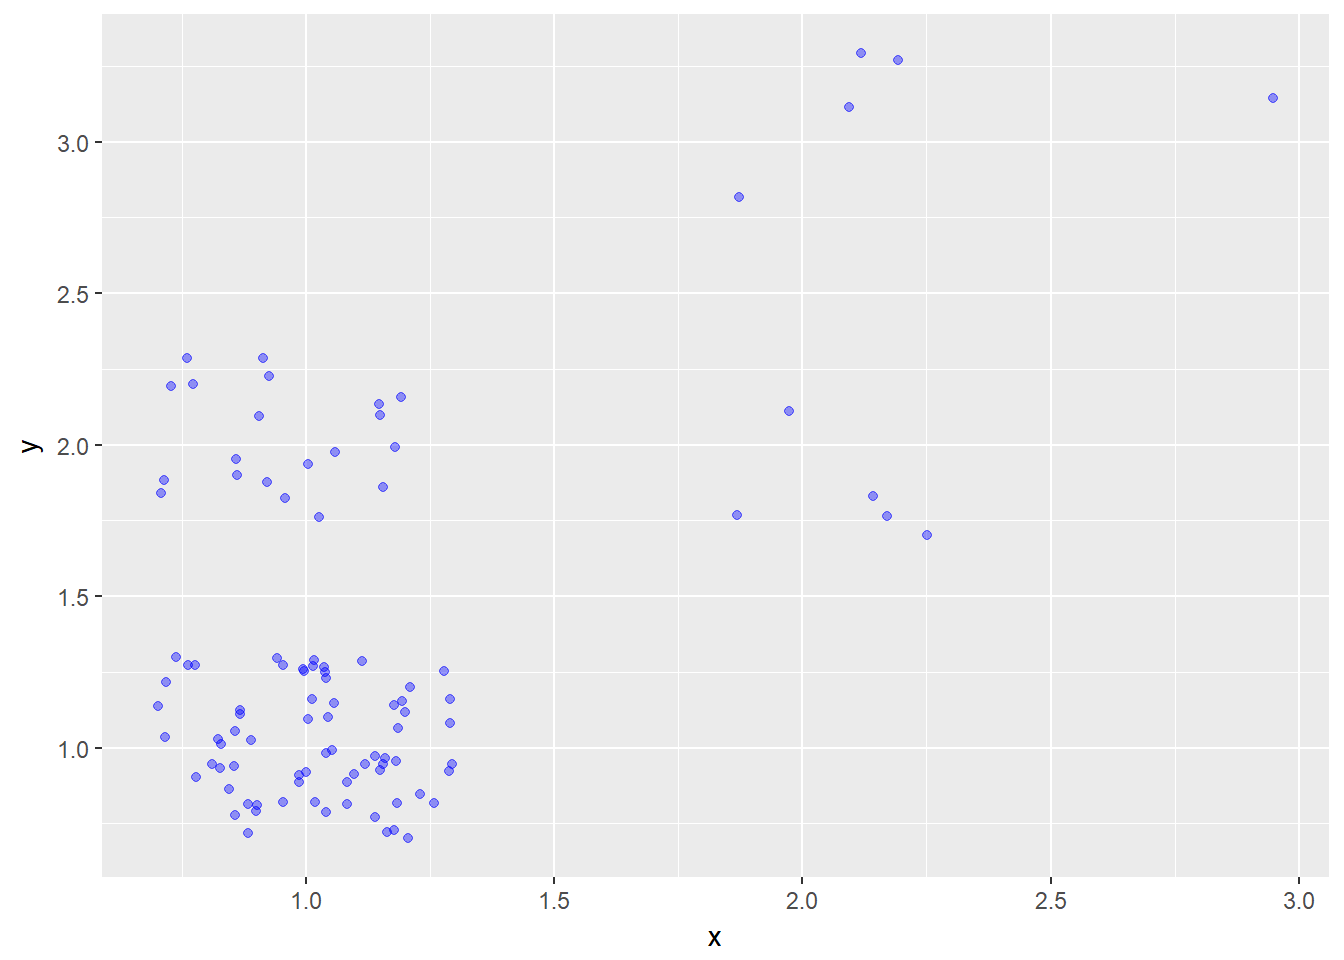
\includegraphics{osnoveR_files/figure-latex/unnamed-chunk-410-1.pdf}

\begin{center}\rule{0.5\linewidth}{\linethickness}\end{center}

\subsubsection{Spremanje slike u
datoteku}\label{spremanje-slike-u-datoteku}

Za kraj ovog dijela naučimo spremiti sliku u datoteku kako bi ju mogli
lako ugraditi u neki drugi izvještajni dokument, znanstveni rad,
proslijediti elektroničkom poštom i sl.

R po default-u koristi zaslon kao ``grafički uređaj'' (engl.
\emph{graphical device}). Opcionalno, grafiku možemo ``preusmjeriti'' na
neki drugi ``uređaj'', najčešće datoteku određenog tipa (\texttt{png},
\texttt{tiff}, \texttt{pdf} i sl.). Popis svih mogućnosti možemo
pogledati uz pomoć naredbe \texttt{?Devices}. Za spremanje grafova u
rasterskom formatu preporučuju se \texttt{png} i \texttt{tiff} formati,
dok je za vektorski format uobičajeno koristiti \texttt{pdf}.

Spremanje grafova može se obaviti pozivom funkcije koja odgovara formatu
u kojeg želimo pohraniti sliku (npr. funkcija \texttt{pdf} spremiti će
\emph{iduću} sliku u \emph{pdf datoteku), no paket \texttt{ggplot2} nudi
nešto praktičniji način - funkcija \texttt{ggsave} pohraniti će }zadnje
iscrtani* graf u datoteku odabranog imena, pri čemu će format slike
zaključiti sama iz ekstenzije datoteke koju odaberemo. Ovaj način je
bolji utoliko što imamo šansu prvo vidjeti graf i tek onda se odlučiti
na pohranu.

\begin{center}\rule{0.5\linewidth}{\linethickness}\end{center}

\textbf{Zadatak 12.21 - spremanje grafa u datoteku}

\begin{Shaded}
\begin{Highlighting}[]
\CommentTok{# spremite sljedeći graf u datoteke `figure1.pdf`i `figure1.png`}
\KeywordTok{ggplot}\NormalTok{(mtcars, }\KeywordTok{aes}\NormalTok{(}\DataTypeTok{x =}\NormalTok{ hp, }\DataTypeTok{y =}\NormalTok{ mpg, }\DataTypeTok{col =} \KeywordTok{as.factor}\NormalTok{(cyl))) }\OperatorTok{+}\StringTok{ }
\StringTok{  }\KeywordTok{geom_point}\NormalTok{() }\OperatorTok{+}\StringTok{ }
\KeywordTok{geom_smooth}\NormalTok{(}\KeywordTok{aes}\NormalTok{(}\DataTypeTok{x =}\NormalTok{ hp, }\DataTypeTok{y =}\NormalTok{ mpg), }\DataTypeTok{method =} \StringTok{'loess'}\NormalTok{, }
            \DataTypeTok{linetype =} \DecValTok{4}\NormalTok{, }\DataTypeTok{color =} \StringTok{"grey"}\NormalTok{, }\DataTypeTok{se =}\NormalTok{ F, }\DataTypeTok{inherit.aes =}\NormalTok{ F) }\OperatorTok{+}
\KeywordTok{labs}\NormalTok{(}\DataTypeTok{x =} \StringTok{"broj konjskih snaga"}\NormalTok{, }\DataTypeTok{y =} \StringTok{"potrošnja"}\NormalTok{, }\DataTypeTok{col =} \StringTok{"broj cilindara"}\NormalTok{)}
\end{Highlighting}
\end{Shaded}

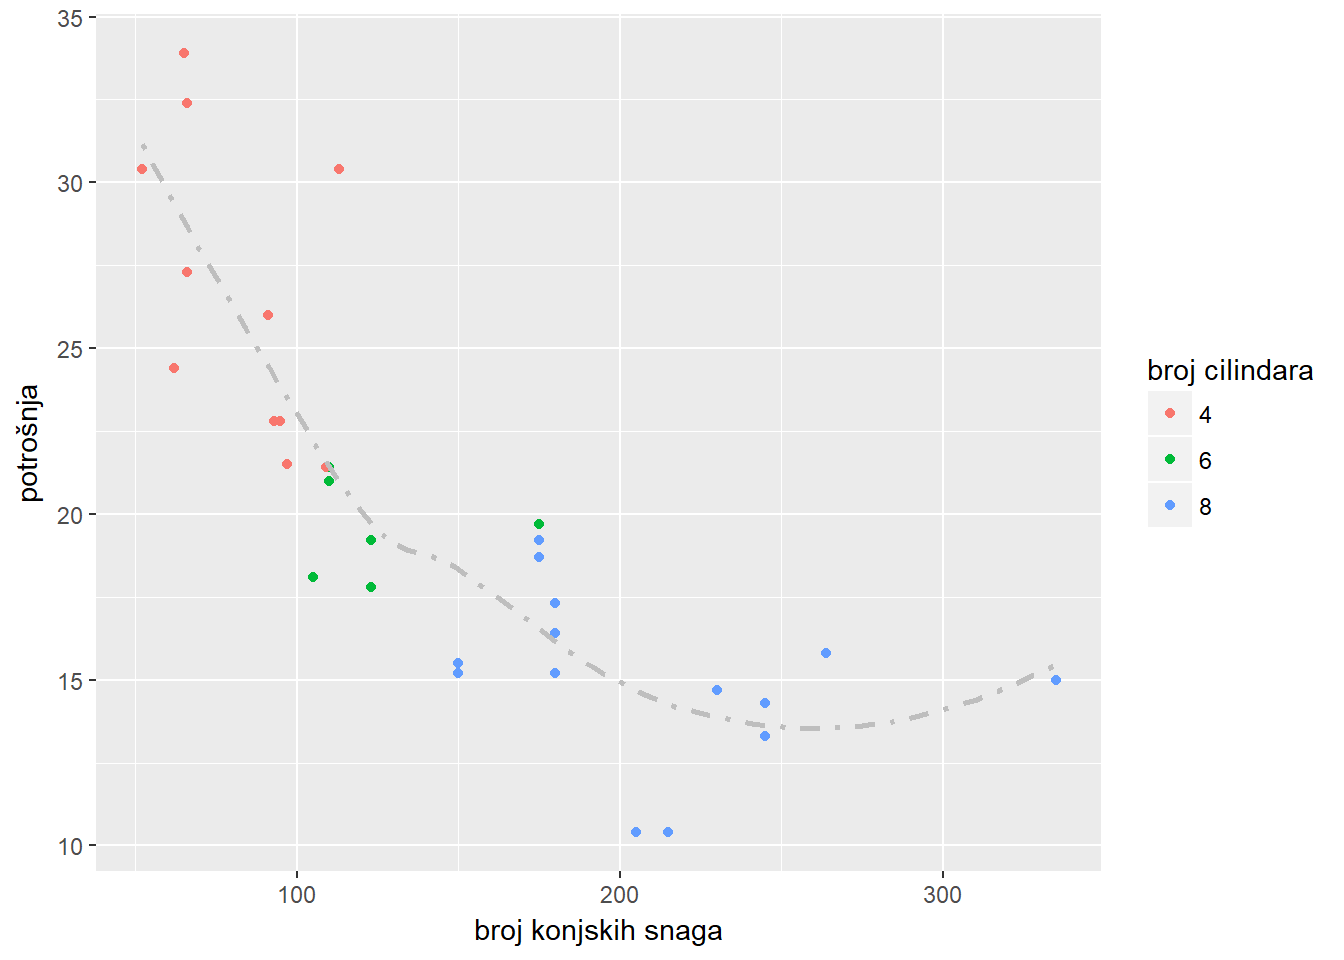
\includegraphics{osnoveR_files/figure-latex/unnamed-chunk-411-1.pdf}

\begin{Shaded}
\begin{Highlighting}[]
\KeywordTok{ggsave}\NormalTok{(}\StringTok{"figure1.pdf"}\NormalTok{)}
\KeywordTok{ggsave}\NormalTok{(}\StringTok{"figure1.png"}\NormalTok{)}
\end{Highlighting}
\end{Shaded}

\begin{center}\rule{0.5\linewidth}{\linethickness}\end{center}

\subsection{Aspekti skale, koordinatnog sustava i
teme}\label{aspekti-skale-koordinatnog-sustava-i-teme}

Već smo ponovili da se stvaranje \texttt{ggplot2} grafova često svodi na
mapiranje stupaca podatkovnog skupa na estetike grafa. \textbf{Skale} su
aspekt koji kontrolira način kako se to mapiranje provodi, tj. metodu
preslikavanja samih podataka na vizualne elemente estetike. U slučaju
koordinatnih osi tu se radi o preslikavanju numeričkih ili kategorijskih
vrijednosti na konkretne udaljenosti na samim osima, dok npr. kod
estetike boje skala odlučuje koja boja označava koju vrijednost
originalnih podataka. Skala je također osnovica za stvaranje legende
grafa.

Ovaj aspekt je do sada uvijek bio implicitno prisutan, ali smo dopuštali
\texttt{ggplot2} paketu da ``odabere'' \emph{default}-ne vrijednosti za
nas. U općenitom slučaju \texttt{ggplot2} relativno dobro kontrolira
aspekt skale neovisno o estetikama koje koristimo, ali vrlo često iz
raznih razloga želimo utjecati na samo mapiranje kako bi npr.
promijenili opseg vrijednosti koje se nalaze na grafu, oznake na osima,
boje ili oblike koji se koriste i sl.

U ovoj lekciji usredotočiti ćemo se samo na one skale koje se relativno
često susreću u praksi. Ostale funkcije i opcije vezane uz aspekte
skaliranje mogu se pronaći u dokumentaciji (ili na \emph{RStudio
ggplot2} podsjetniku).

\begin{center}\rule{0.5\linewidth}{\linethickness}\end{center}

Kada radimo sa skalama, najčešće se koristimo ovim pomoćnim funkcijama
(\texttt{*} predstavlja ``ime estetike'', kao npr. \texttt{x},
\texttt{y}, \texttt{color} itd.):

\begin{itemize}
\tightlist
\item
  \texttt{scale\_*\_continuous} - za mapiranje kontinuiranih
  (numeričkih) vrijednosti
\item
  \texttt{scale\_*\_discrete} - za mapiranje diskretnih vrijednosti
\end{itemize}

Svaka od ovih funkcija ima niz parametara koje možemo koristiti kako bi
utjecali na postupak mapiranja. Npr. ako pogledamo dokumentaciju za
\texttt{scale\_x\_continuous} možemo vidjeti da između ostalog možemo
postaviti parametre:

\begin{itemize}
\tightlist
\item
  \texttt{name} - ime skale koje ujedno postaje i naziv osi/legende
\item
  \texttt{breaks} - na kojim pozicijama se stavljaju crtice
\item
  \texttt{labels} - koje vrijednosti se ispisuju ispod crtica
\item
  \texttt{limits} - raspon vrijednosti koji će se nalaziti na osi
\item
  itd.
\end{itemize}

Važno je napomenuti da \texttt{ggplot2} ima puno dodatnih pomoćnih
funkcija koje omogućuju da na neke od ovih stvari podešavamo i mimo
funkcija skaliranja, kao npr. već viđeni \texttt{labs} s kojim smo
preimenovali naziv grafa, osi i legendi, ali također i funkcije
\texttt{xlim}/\texttt{ylim} kojima utječemo samo na raspon osi i sl.
Često se isplati pomno pogledati dokumentaciju budući da se mogu naći
zgodne funkcije koje nam uvelike olakšavaju posao skraćivanjem sintakse
za vizualizacijske zadatke koje obavljamo.

Isprobajmo neke od navedenih funkcija na primjerima. Koristiti ćemo se
podatkovnim skupom \texttt{diamonds} paketa \texttt{ggplot2}, kojeg smo
upoznali u zadacima za vježbu iz prethodne lekcije, a koji opisuje
značajke dijamanata uz njihovu procijenjenu vrijednost.

\begin{center}\rule{0.5\linewidth}{\linethickness}\end{center}

\textbf{Zadatak 12.22 - upoznavanje sa podatkovnim skupom `diamonds'}

\begin{Shaded}
\begin{Highlighting}[]
\CommentTok{# proučite podatkovni okvir `diamonds`}
\end{Highlighting}
\end{Shaded}

\begin{Shaded}
\begin{Highlighting}[]
\CommentTok{# proučite podatkovni okvir `diamonds`}
\KeywordTok{glimpse}\NormalTok{(diamonds)}
\KeywordTok{head}\NormalTok{(diamonds)}
\end{Highlighting}
\end{Shaded}

\begin{verbatim}
## Observations: 53,940
## Variables: 10
## $ carat   <dbl> 0.23, 0.21, 0.23, 0.29, 0.31, 0.24, 0.24, 0.26, 0.22, ...
## $ cut     <ord> Ideal, Premium, Good, Premium, Good, Very Good, Very G...
## $ color   <ord> E, E, E, I, J, J, I, H, E, H, J, J, F, J, E, E, I, J, ...
## $ clarity <ord> SI2, SI1, VS1, VS2, SI2, VVS2, VVS1, SI1, VS2, VS1, SI...
## $ depth   <dbl> 61.5, 59.8, 56.9, 62.4, 63.3, 62.8, 62.3, 61.9, 65.1, ...
## $ table   <dbl> 55, 61, 65, 58, 58, 57, 57, 55, 61, 61, 55, 56, 61, 54...
## $ price   <int> 326, 326, 327, 334, 335, 336, 336, 337, 337, 338, 339,...
## $ x       <dbl> 3.95, 3.89, 4.05, 4.20, 4.34, 3.94, 3.95, 4.07, 3.87, ...
## $ y       <dbl> 3.98, 3.84, 4.07, 4.23, 4.35, 3.96, 3.98, 4.11, 3.78, ...
## $ z       <dbl> 2.43, 2.31, 2.31, 2.63, 2.75, 2.48, 2.47, 2.53, 2.49, ...
## # A tibble: 6 x 10
##   carat       cut color clarity depth table price     x     y     z
##   <dbl>     <ord> <ord>   <ord> <dbl> <dbl> <int> <dbl> <dbl> <dbl>
## 1  0.23     Ideal     E     SI2  61.5    55   326  3.95  3.98  2.43
## 2  0.21   Premium     E     SI1  59.8    61   326  3.89  3.84  2.31
## 3  0.23      Good     E     VS1  56.9    65   327  4.05  4.07  2.31
## 4  0.29   Premium     I     VS2  62.4    58   334  4.20  4.23  2.63
## 5  0.31      Good     J     SI2  63.3    58   335  4.34  4.35  2.75
## 6  0.24 Very Good     J    VVS2  62.8    57   336  3.94  3.96  2.48
\end{verbatim}

\begin{center}\rule{0.5\linewidth}{\linethickness}\end{center}

\textbf{Zadatak 12.23 - uzorkovanje skupa `diamonds'}

\begin{Shaded}
\begin{Highlighting}[]
\KeywordTok{set.seed}\NormalTok{(}\DecValTok{1001}\NormalTok{)}
\CommentTok{# stvorite okvir `diamondsSample` u koji ćete staviti}
\CommentTok{# 5000 nasumičnih redaka iz okvira `diamonds`}
\end{Highlighting}
\end{Shaded}

\begin{Shaded}
\begin{Highlighting}[]
\KeywordTok{set.seed}\NormalTok{(}\DecValTok{1001}\NormalTok{)}
\CommentTok{# stvorite okvir `diamondsSample` u koji ćete staviti}
\CommentTok{# 5000 nasumičnih redaka iz okvira `diamonds`}
\NormalTok{diamondsSample <-}\StringTok{ }\KeywordTok{sample_n}\NormalTok{(diamonds, }\DecValTok{5000}\NormalTok{)}
\end{Highlighting}
\end{Shaded}

\begin{center}\rule{0.5\linewidth}{\linethickness}\end{center}

\textbf{Zadatak 12.24 - korištenje aspekta skale}

\begin{Shaded}
\begin{Highlighting}[]
\CommentTok{# "popravite" osi i legendu grafa koji prikazuje ovisnost }
\CommentTok{# veličine dijamanta, boje i cijene}
\CommentTok{# - osi x i y nazovite "volumen u mm3" i "cijena u $"}
\CommentTok{# - legendu nazovite "kvaliteta boje"}
\CommentTok{# - os x ograničite od 0 do 500}
\CommentTok{# - na osi y postavite crtice na 1000, 5000, 10000 i 20000}
\CommentTok{# - kategorije kvalitete boje postavite na brojeve }
\CommentTok{# od 1 do 7 gdje 1 predstavlja "najbolju" boju}
\KeywordTok{ggplot}\NormalTok{(diamondsSample, }\KeywordTok{aes}\NormalTok{(x}\OperatorTok{*}\NormalTok{y}\OperatorTok{*}\NormalTok{z, price, }\DataTypeTok{color =}\NormalTok{ color)) }\OperatorTok{+}\StringTok{ }\KeywordTok{geom_point}\NormalTok{(}\DataTypeTok{alpha =} \FloatTok{0.4}\NormalTok{) }
\end{Highlighting}
\end{Shaded}

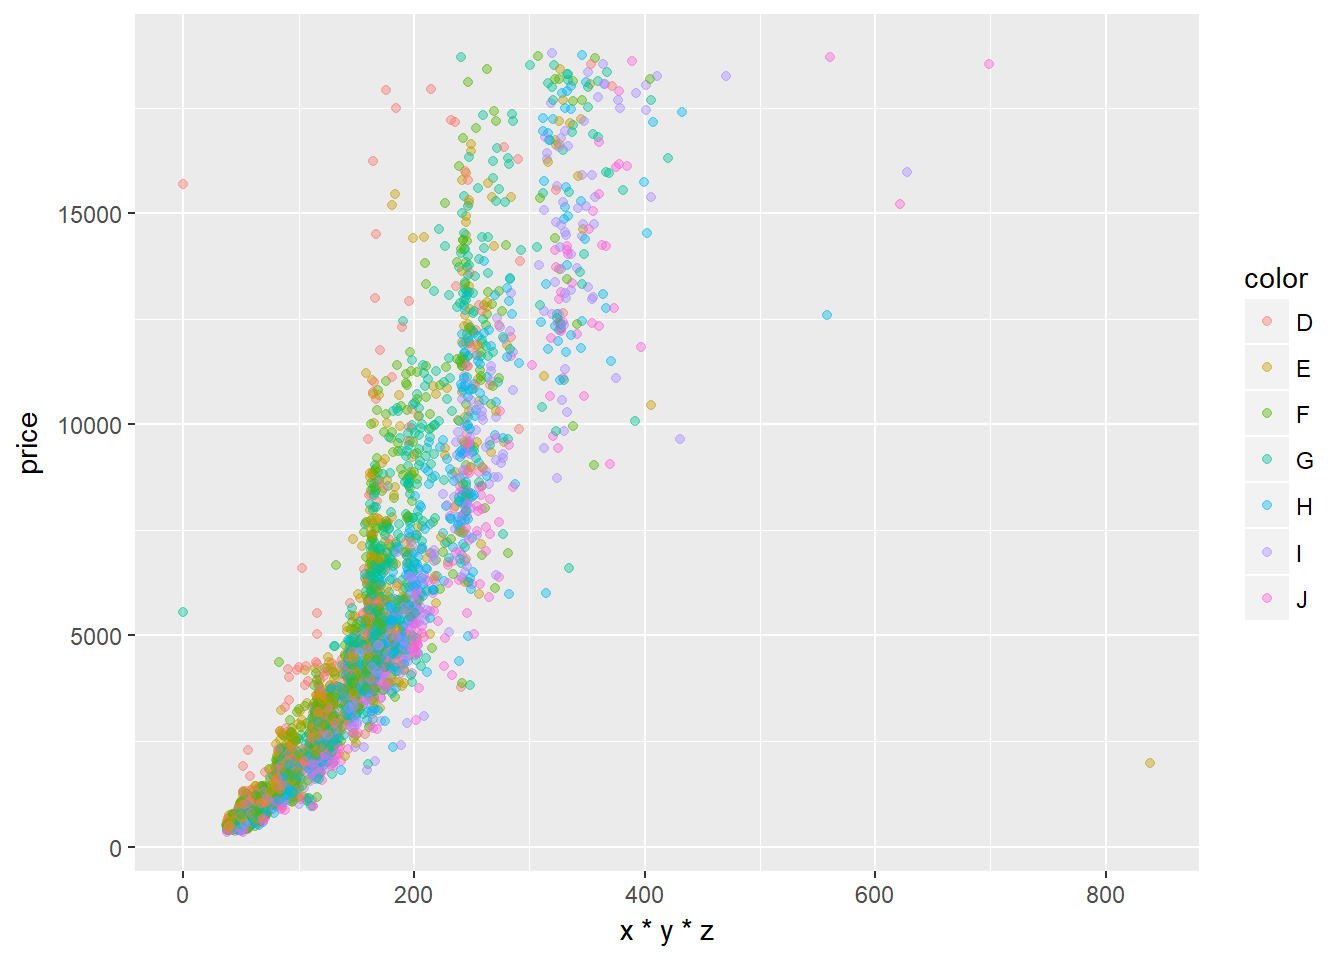
\includegraphics{osnoveR_files/figure-latex/unnamed-chunk-417-1.pdf}

\begin{Shaded}
\begin{Highlighting}[]
\KeywordTok{ggplot}\NormalTok{(diamondsSample, }\KeywordTok{aes}\NormalTok{(x}\OperatorTok{*}\NormalTok{y}\OperatorTok{*}\NormalTok{z, price, }\DataTypeTok{color =}\NormalTok{ color)) }\OperatorTok{+}\StringTok{ }
\StringTok{  }\KeywordTok{geom_point}\NormalTok{(}\DataTypeTok{alpha =} \FloatTok{0.6}\NormalTok{) }\OperatorTok{+}
\StringTok{  }\KeywordTok{scale_x_continuous}\NormalTok{(}\DataTypeTok{name =} \StringTok{"volumen u mm3"}\NormalTok{ , }\DataTypeTok{limits =} \KeywordTok{c}\NormalTok{(}\DecValTok{0}\NormalTok{, }\DecValTok{450}\NormalTok{)) }\OperatorTok{+}
\StringTok{  }\KeywordTok{scale_y_continuous}\NormalTok{(}\DataTypeTok{name =} \StringTok{"cijena u $"}\NormalTok{, }
                     \DataTypeTok{breaks =} \KeywordTok{c}\NormalTok{(}\DecValTok{1000}\NormalTok{, }\DecValTok{5000}\NormalTok{, }\DecValTok{10000}\NormalTok{, }\DecValTok{15000}\NormalTok{)) }\OperatorTok{+}
\StringTok{  }\KeywordTok{scale_color_discrete}\NormalTok{(}\DataTypeTok{name =} \StringTok{"kvaliteta boje"}\NormalTok{, }\DataTypeTok{labels =} \DecValTok{1}\OperatorTok{:}\DecValTok{7}\NormalTok{)}
\end{Highlighting}
\end{Shaded}

\begin{verbatim}
## Warning: Removed 7 rows containing missing values (geom_point).
\end{verbatim}

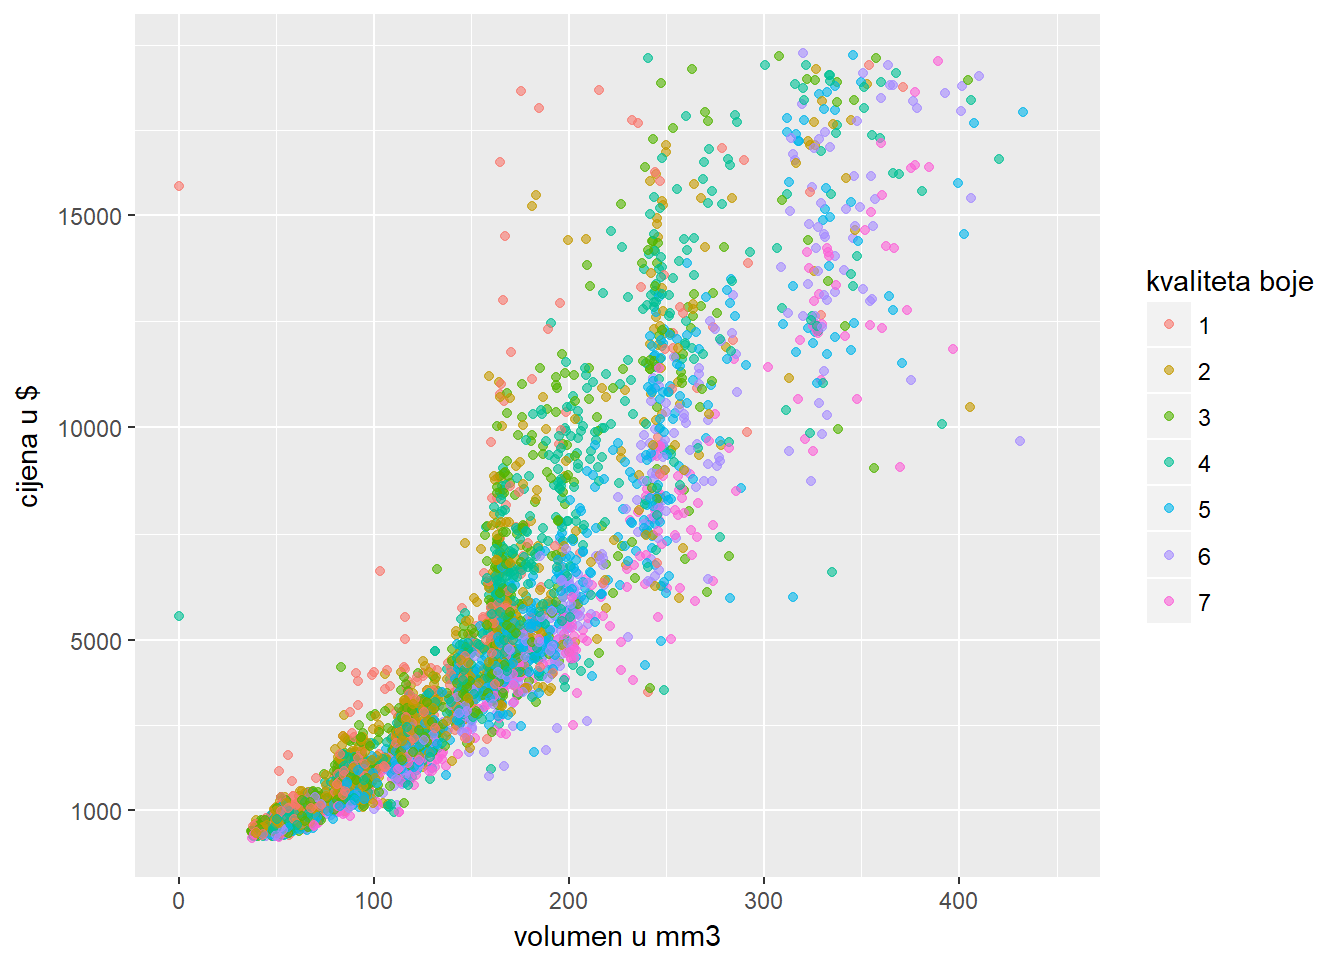
\includegraphics{osnoveR_files/figure-latex/unnamed-chunk-418-1.pdf}

\begin{center}\rule{0.5\linewidth}{\linethickness}\end{center}

Uočite kako \texttt{ggplot} za svaki slučaj javlja kako neke obzervacije
nisu prikazane. Ukoliko želimo spriječiti ovo upozorenje, dovoljno je
dodati argument \texttt{na.rm\ =\ T} u sloj geometrije.

Vrlo često se događa da na grafovima uočavamo tzv. ``eksponencijalni
trend'', tj. da nas ovisnost jedna varijable u drugoj podsjeća na
eksponencijalnu funkciju. Prethodni graf također je primjer takvog
scenarija - može se primijetiti da cijena dijamanta na početku ``blago''
raste sa veličinom dijamanta, da bi kasnije počela strmije rasti.

U analizi podataka u ovakvim slučajevima često provodimo transformacije
podataka - npr. u ovom slučaju mogli bismo logaritmirati cijenu kako bi
eksponencijalni trend pretvorili u linearni kojeg u općenitom slučaju
preferiramo. No transformacija cijene u logaritam nosi sa sobom problem
interpretacije - graf bolje komunicira informaciju ako se na njemu
nalazi doslovni, a ne izvedeni podatak (1000 dolara naspram 3
``logaritma od dolara'').

Skale nam u ovome slučaju mogu pomoći - umjesto da ``diramo'' podatke,
mi jednostavno koristimo logaritmiranu (ili neku drugu) skalu.
Konkretno, umjesto funkcije \texttt{scale\_*\_continuous} možemo
odabrati:

\begin{itemize}
\tightlist
\item
  \texttt{scale\_*\_log10} - logaritmira skalu po bazi 10
\item
  \texttt{scale\_*\_reverse} - ``obrće'' skalu s desna na lijevo
\item
  \texttt{scale\_*\_sqrt} - ``korjenuje'' vrijednosti skale
\end{itemize}

\begin{center}\rule{0.5\linewidth}{\linethickness}\end{center}

\textbf{Zadatak 12.25 - logaritamska skala}

\begin{Shaded}
\begin{Highlighting}[]
\CommentTok{# logaritmirajte cijenu dijamanta u prethodno izvedenom grafu}
\KeywordTok{ggplot}\NormalTok{(diamondsSample, }\KeywordTok{aes}\NormalTok{(x}\OperatorTok{*}\NormalTok{y}\OperatorTok{*}\NormalTok{z, price, }\DataTypeTok{color =}\NormalTok{ color)) }\OperatorTok{+}\StringTok{ }\KeywordTok{geom_point}\NormalTok{(}\DataTypeTok{na.rm =}\NormalTok{ T, }\DataTypeTok{alpha =} \FloatTok{0.6}\NormalTok{) }\OperatorTok{+}
\StringTok{  }\KeywordTok{scale_x_continuous}\NormalTok{(}\DataTypeTok{name =} \StringTok{"volumen u mm3"}\NormalTok{ , }\DataTypeTok{limits =} \KeywordTok{c}\NormalTok{(}\DecValTok{0}\NormalTok{, }\DecValTok{450}\NormalTok{)) }\OperatorTok{+}
\StringTok{  }\KeywordTok{scale_y_continuous}\NormalTok{(}\DataTypeTok{name =} \StringTok{"cijena u $"}\NormalTok{, }\DataTypeTok{breaks =} \KeywordTok{c}\NormalTok{(}\DecValTok{1000}\NormalTok{, }\DecValTok{5000}\NormalTok{, }\DecValTok{10000}\NormalTok{, }\DecValTok{15000}\NormalTok{)) }\OperatorTok{+}
\StringTok{  }\KeywordTok{scale_color_discrete}\NormalTok{(}\DataTypeTok{name =} \StringTok{"kvaliteta boje"}\NormalTok{, }\DataTypeTok{labels =} \DecValTok{1}\OperatorTok{:}\DecValTok{7}\NormalTok{)}
\end{Highlighting}
\end{Shaded}

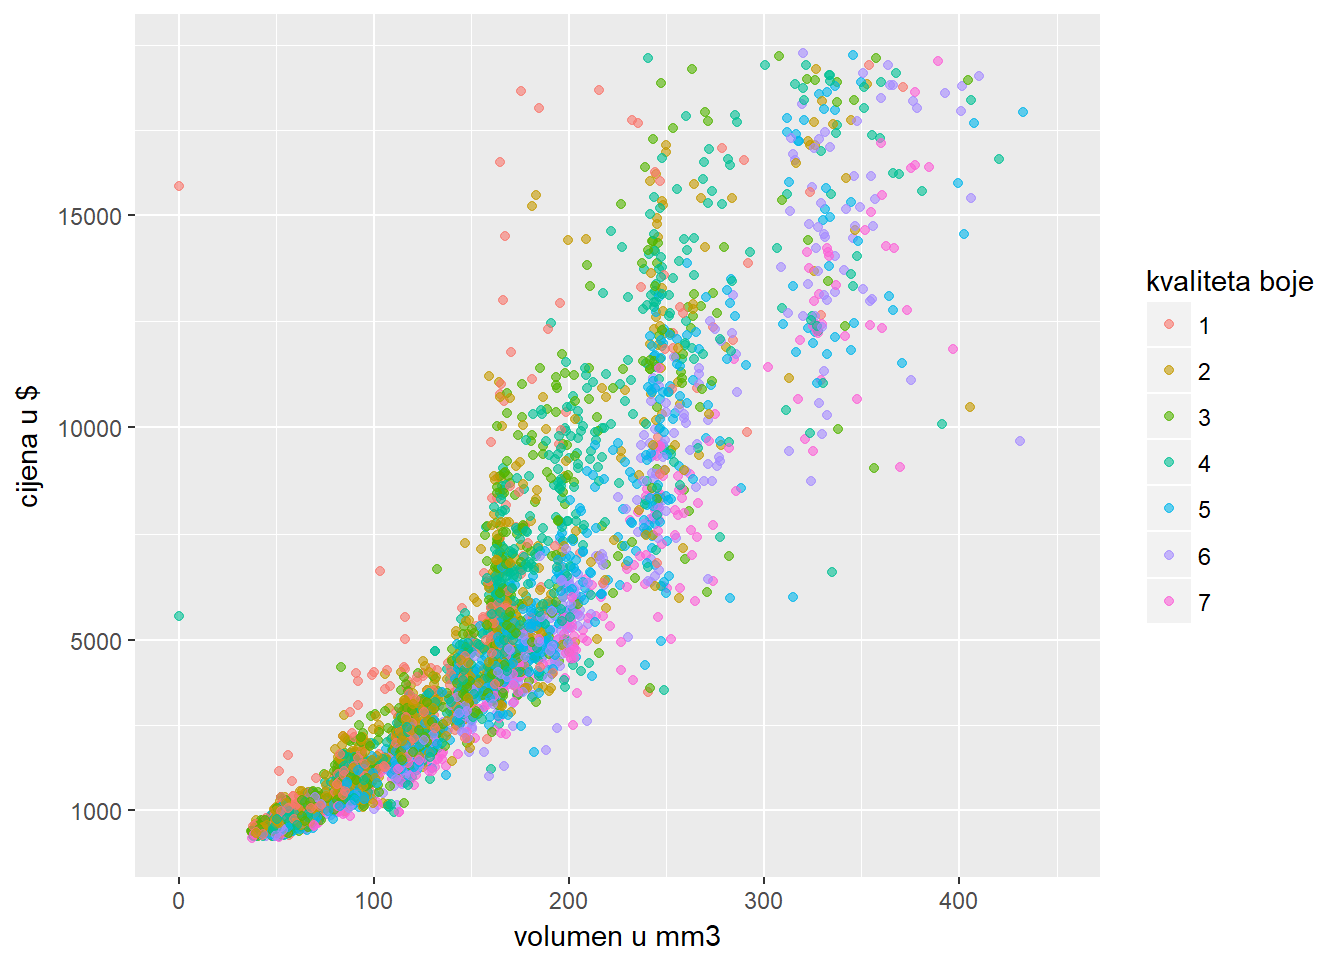
\includegraphics{osnoveR_files/figure-latex/unnamed-chunk-419-1.pdf}

\begin{Shaded}
\begin{Highlighting}[]
\CommentTok{# logaritmirajte cijenu dijamanta u prethodno izvedenom grafu}
\KeywordTok{ggplot}\NormalTok{(diamondsSample, }\KeywordTok{aes}\NormalTok{(x}\OperatorTok{*}\NormalTok{y}\OperatorTok{*}\NormalTok{z, price, }\DataTypeTok{color =}\NormalTok{ color)) }\OperatorTok{+}\StringTok{ }
\StringTok{  }\KeywordTok{geom_point}\NormalTok{(}\DataTypeTok{na.rm =}\NormalTok{ T, }\DataTypeTok{alpha =} \FloatTok{0.6}\NormalTok{) }\OperatorTok{+}
\StringTok{  }\KeywordTok{scale_x_continuous}\NormalTok{(}\DataTypeTok{name =} \StringTok{"volumen u mm3"}\NormalTok{ , }\DataTypeTok{limits =} \KeywordTok{c}\NormalTok{(}\DecValTok{0}\NormalTok{, }\DecValTok{450}\NormalTok{)) }\OperatorTok{+}
\StringTok{  }\KeywordTok{scale_y_log10}\NormalTok{(}\DataTypeTok{name =} \StringTok{"cijena u $"}\NormalTok{, }
                \DataTypeTok{breaks =} \KeywordTok{c}\NormalTok{(}\DecValTok{1000}\NormalTok{, }\DecValTok{5000}\NormalTok{, }\DecValTok{10000}\NormalTok{, }\DecValTok{15000}\NormalTok{)) }\OperatorTok{+}
\StringTok{  }\KeywordTok{scale_color_discrete}\NormalTok{(}\DataTypeTok{name =} \StringTok{"kvaliteta boje"}\NormalTok{, }\DataTypeTok{labels =} \DecValTok{1}\OperatorTok{:}\DecValTok{7}\NormalTok{)}
\end{Highlighting}
\end{Shaded}

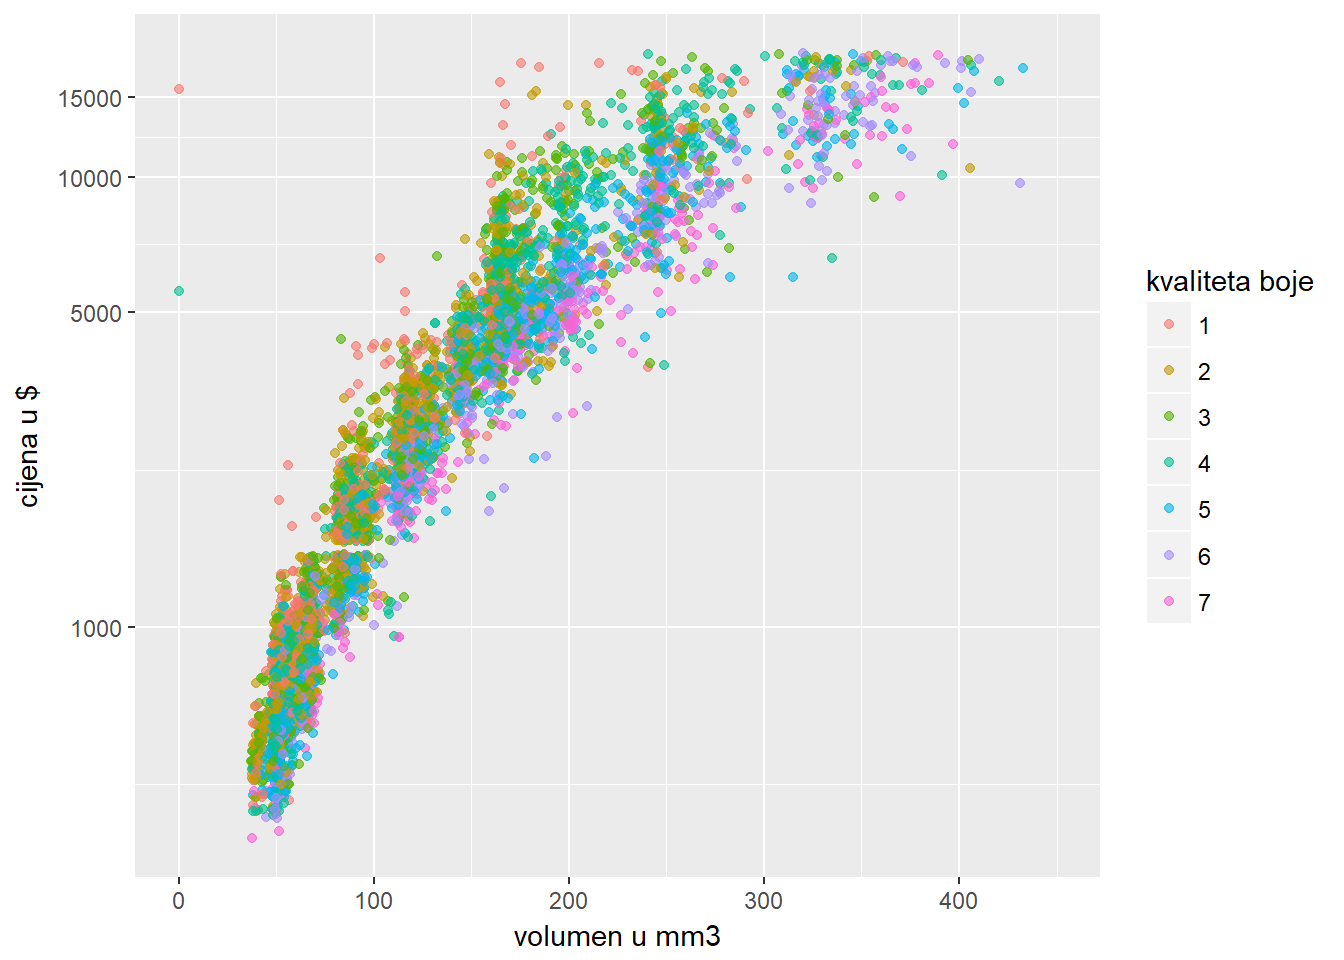
\includegraphics{osnoveR_files/figure-latex/unnamed-chunk-420-1.pdf}

\begin{center}\rule{0.5\linewidth}{\linethickness}\end{center}

Jedna stvar koju vrlo često volimo ``popravljati'' na grafovima su boje
- bilo da želimo bolje naglasiti informacije koje graf prenosi, uklopiti
graf u okolinu u kojoj se nalazi, ili jednostavno želimo da nam graf
koristi boje koje nalazimo estetski ugodnima. Upravo zbog toga estetike
\texttt{color} i \texttt{fill} se vrlo često dodatno podešavaju uz pomoć
skala. Za ovo imamo zgodne funkcije (dajemo primjere za \texttt{fill}
estetike iako većina funkcija postoji i za \texttt{color}):

\begin{itemize}
\tightlist
\item
  \texttt{scale\_fill\_brewer} - odabir jedne od unaprijed pripremljenih
  paleta boja namijenjenih prikazu diskretnih vrijednosti; imena paleta
  mogu se pogledati u dokumentaciji
\item
  \texttt{scale\_fill\_distiller} - prilagođava palete za diskretne
  vrijednosti kontinuiranim varijablama
\item
  \texttt{scale\_fill\_gradient} - odabir početne i konačne boje koje će
  se ``prelijevati'' jedna u drugu; koristimo za prikaz kontinuiranih
  vrijednosti
\item
  \texttt{scale\_fill\_gradient2}, \texttt{scale\_fill\_gradientn} - ako
  želimo više ``prelijevanja''
\item
  \texttt{scale\_fill\_grey} - za crno bijele vizualizacije
\end{itemize}

\begin{center}\rule{0.5\linewidth}{\linethickness}\end{center}

\textbf{Zadatak 12.26 - prilagodba boja na grafu}

\begin{Shaded}
\begin{Highlighting}[]
\CommentTok{# podesite `fill` estetiku sljedećeg grafa korištenjem }
\CommentTok{# funkcije `scale_fill_brewer`}
\CommentTok{# parametar `palette` postavite na jednu od sljedećih paleta:}
\CommentTok{# Blues, BuPu, Greens, Greys, Oranges, OrRd, PuBu, }
\CommentTok{#     PuRd, Purples, YlGn, YlOrRd}
\CommentTok{# (još paleta možete naći u dokumentaciji)}
\KeywordTok{ggplot}\NormalTok{(diamondsSample, }\KeywordTok{aes}\NormalTok{(}\DataTypeTok{x =}\NormalTok{ x}\OperatorTok{*}\NormalTok{y}\OperatorTok{*}\NormalTok{z, }\DataTypeTok{fill =}\NormalTok{ color)) }\OperatorTok{+}\StringTok{ }
\StringTok{  }\KeywordTok{geom_histogram}\NormalTok{(}\DataTypeTok{bins =} \DecValTok{30}\NormalTok{, }\DataTypeTok{na.rm =}\NormalTok{ T) }\OperatorTok{+}\StringTok{ }
\StringTok{  }\KeywordTok{xlim}\NormalTok{(}\DecValTok{0}\NormalTok{, }\DecValTok{500}\NormalTok{)}
\end{Highlighting}
\end{Shaded}

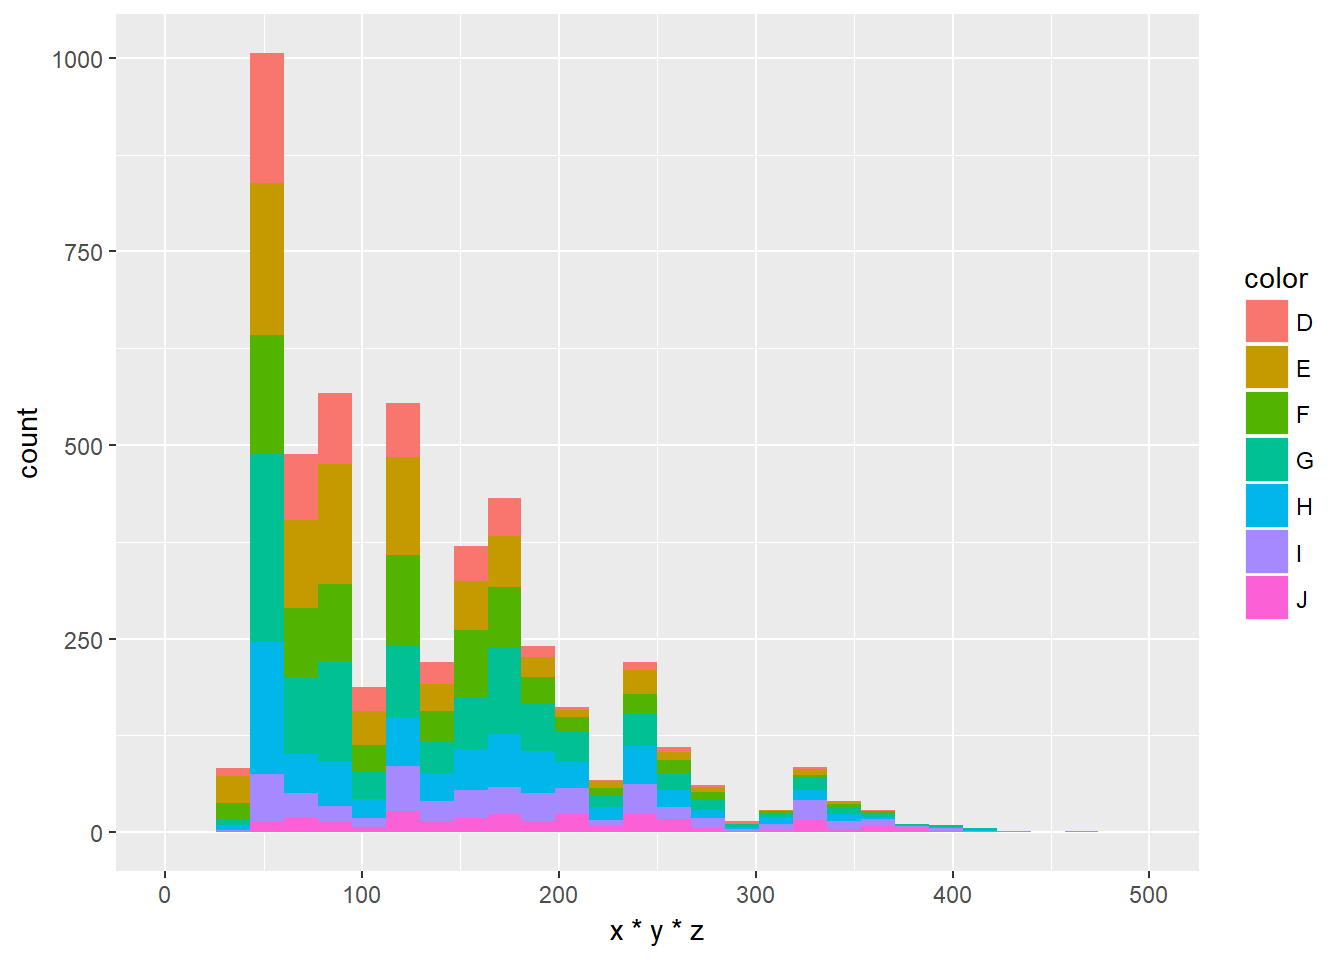
\includegraphics{osnoveR_files/figure-latex/unnamed-chunk-421-1.pdf}

\begin{Shaded}
\begin{Highlighting}[]
\CommentTok{# podesite `fill` estetiku sljedećeg grafa korištenjem }
\CommentTok{# funkcije `scale_fill_brewer`}
\CommentTok{# parametar `palette` postavite na jednu od sljedećih paleta:}
\CommentTok{# Blues, BuPu, Greens, Greys, Oranges, OrRd, PuBu, }
\CommentTok{#      PuRd, Purples, YlGn, YlOrRd}
\CommentTok{# (još paleta možete naći u dokumentaciji)}
\KeywordTok{ggplot}\NormalTok{(diamondsSample, }\KeywordTok{aes}\NormalTok{(}\DataTypeTok{x =}\NormalTok{ x}\OperatorTok{*}\NormalTok{y}\OperatorTok{*}\NormalTok{z, }\DataTypeTok{fill =}\NormalTok{ color)) }\OperatorTok{+}\StringTok{ }
\StringTok{  }\KeywordTok{geom_histogram}\NormalTok{(}\DataTypeTok{bins =} \DecValTok{30}\NormalTok{, }\DataTypeTok{na.rm =}\NormalTok{ T) }\OperatorTok{+}\StringTok{ }
\StringTok{  }\KeywordTok{xlim}\NormalTok{(}\DecValTok{0}\NormalTok{, }\DecValTok{500}\NormalTok{) }\OperatorTok{+}\StringTok{ }\KeywordTok{scale_fill_brewer}\NormalTok{(}\DataTypeTok{palette =} \StringTok{"Greens"}\NormalTok{)}
\end{Highlighting}
\end{Shaded}

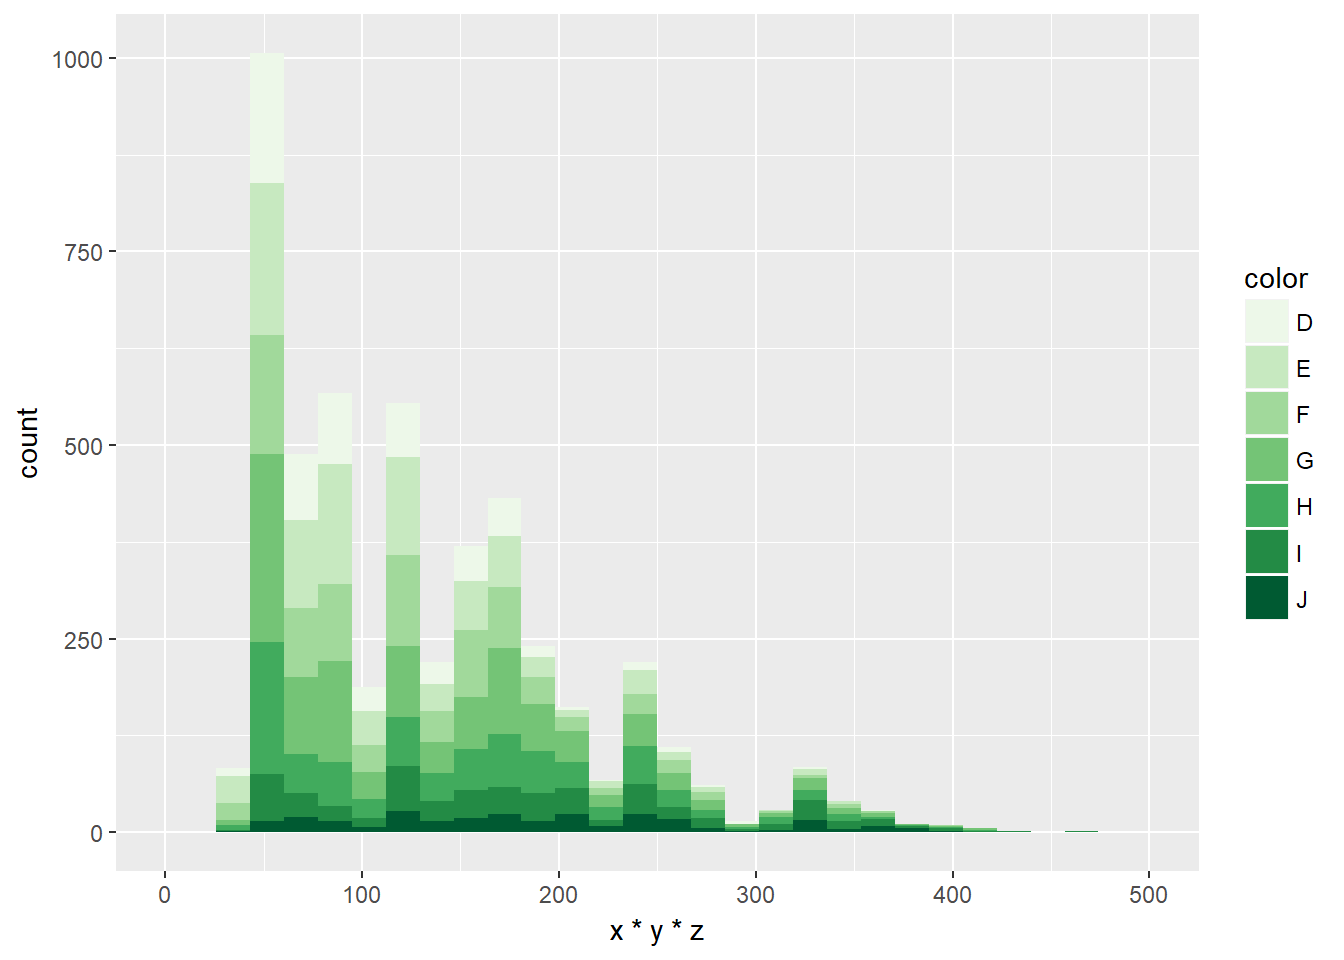
\includegraphics{osnoveR_files/figure-latex/unnamed-chunk-422-1.pdf}

\begin{Shaded}
\begin{Highlighting}[]
\CommentTok{# podesite `fill` estetiku sljedećeg grafa korištenjem }
\CommentTok{# funkcije `scale_fill_brewer`}
\CommentTok{# parametar `palette` postavite na jednu od sljedećih paleta:}
\CommentTok{# Blues, BuPu, Greens, Greys, Oranges, OrRd, PuBu, }
\CommentTok{#   PuRd, Purples, YlGn, YlOrRd}
\CommentTok{# (još paleta možete naći u dokumentaciji)}
\KeywordTok{ggplot}\NormalTok{(diamondsSample, }\KeywordTok{aes}\NormalTok{(}\DataTypeTok{x =}\NormalTok{ x}\OperatorTok{*}\NormalTok{y}\OperatorTok{*}\NormalTok{z, }\DataTypeTok{fill =}\NormalTok{ color)) }\OperatorTok{+}\StringTok{ }
\StringTok{  }\KeywordTok{geom_histogram}\NormalTok{(}\DataTypeTok{bins =} \DecValTok{30}\NormalTok{, }\DataTypeTok{na.rm =}\NormalTok{ T) }\OperatorTok{+}\StringTok{ }
\StringTok{  }\KeywordTok{xlim}\NormalTok{(}\DecValTok{0}\NormalTok{, }\DecValTok{500}\NormalTok{) }\OperatorTok{+}\StringTok{ }\KeywordTok{scale_fill_brewer}\NormalTok{(}\DataTypeTok{palette =} \StringTok{"YlOrRd"}\NormalTok{)}
\end{Highlighting}
\end{Shaded}

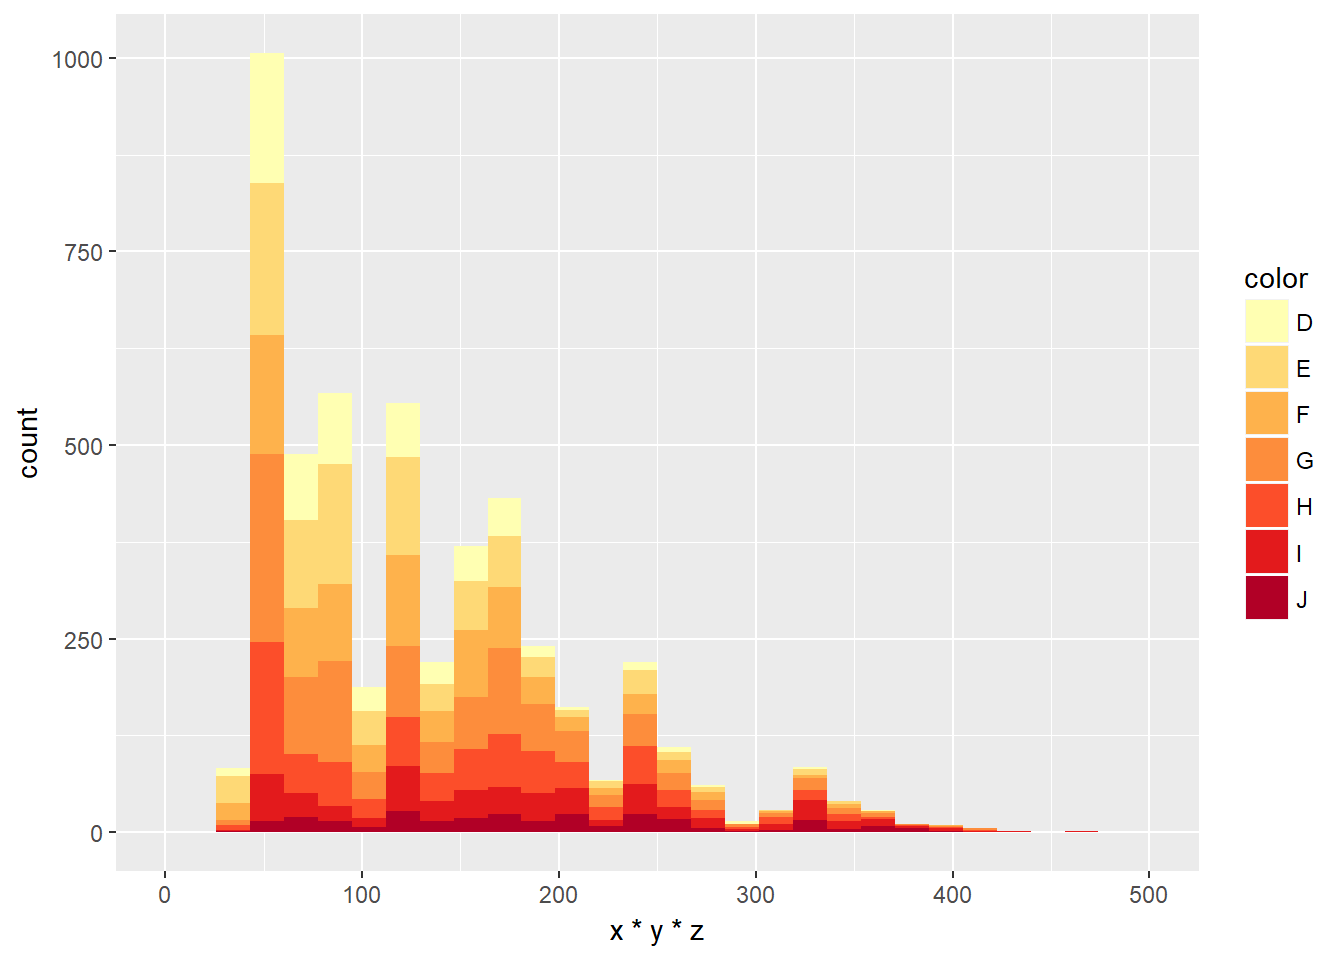
\includegraphics{osnoveR_files/figure-latex/unnamed-chunk-423-1.pdf}

\begin{center}\rule{0.5\linewidth}{\linethickness}\end{center}

Aspekt \textbf{koordinatnog sustava} vrlo rijetko mijenjamo. Razlog tome
je što u najvećem broju slučajeva želimo koristiti Kartezijev
koordinatni sustav koji \texttt{ggplot} koristi po \emph{default}-u.
Ukoliko smatramo da naša vizualizacija zahtijeva nešto drugo - bilo da
se radi o polarnom koordinatnom sustavu, ili želimo ``izvrnuti'' naš
Kartezijev sustav na stranu, ili - što je posebno važno kod analize
zemljopisnih podataka - želimo da naša vizualizacija prikazuje
zemljopisnu kartu, možemo između ostalog koristiti sljedeće funkcije:

\begin{itemize}
\tightlist
\item
  \texttt{coord\_polar} - polarni koordinatni sustav
\item
  \texttt{coord\_flip} - mijenja \texttt{x} i \texttt{y} osi
\item
  \texttt{coord\_map} - koristi karte iz paketa \texttt{maps} i
  \texttt{mapproj}
\end{itemize}

Trenutno nažalost još ne postoje karte Republike Hrvatske, no
ambiciozniji čitatelji mogu pokušati stvoriti istu (i podijeliti sa
lokalnom R zajednicom) prateći upute na ovoj i ovoj poveznici.

\begin{center}\rule{0.5\linewidth}{\linethickness}\end{center}

\textbf{Zadatak 12.27 - izvrnuti i polarni koordinatni sustavi}

\begin{Shaded}
\begin{Highlighting}[]
\CommentTok{# pogledajte kako sljedeći graf izgleda u "izvrnutom" a kako u polarnom koordinatnom sustavu}
\KeywordTok{ggplot}\NormalTok{(diamondsSample, }\KeywordTok{aes}\NormalTok{(}\DataTypeTok{x =}\NormalTok{ x}\OperatorTok{*}\NormalTok{y}\OperatorTok{*}\NormalTok{z, }\DataTypeTok{fill =}\NormalTok{ color)) }\OperatorTok{+}\StringTok{ }\KeywordTok{geom_histogram}\NormalTok{(}\DataTypeTok{bins =} \DecValTok{30}\NormalTok{, }\DataTypeTok{na.rm =}\NormalTok{ T) }\OperatorTok{+}\StringTok{ }
\StringTok{  }\KeywordTok{xlim}\NormalTok{(}\DecValTok{40}\NormalTok{, }\DecValTok{100}\NormalTok{) }
\end{Highlighting}
\end{Shaded}

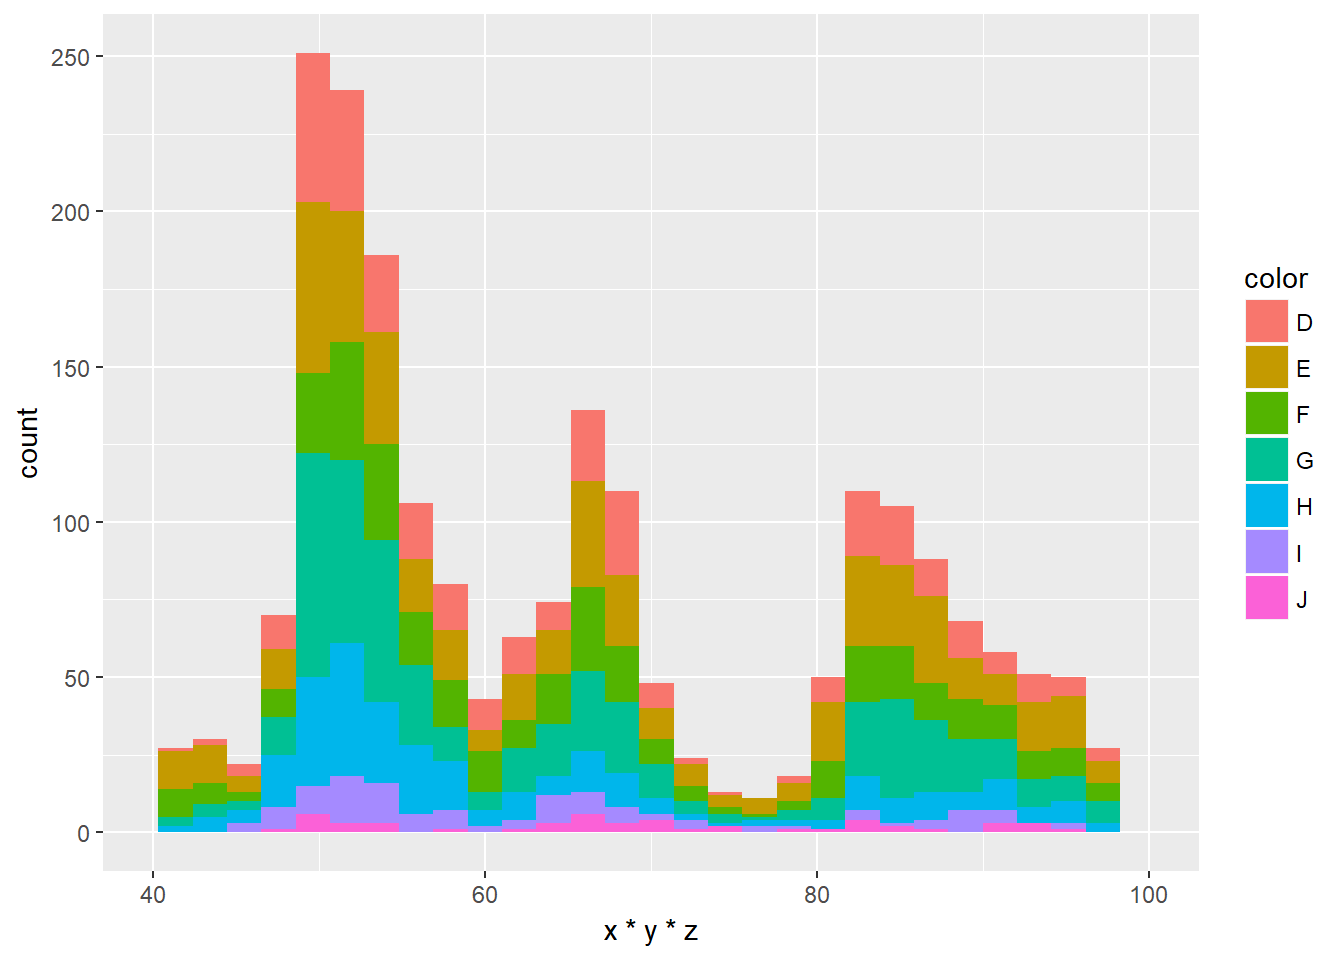
\includegraphics{osnoveR_files/figure-latex/unnamed-chunk-424-1.pdf}

\begin{Shaded}
\begin{Highlighting}[]
\CommentTok{# pogledajte kako sljedeći graf izgleda u "izvrnutom" }
\CommentTok{# a kako u polarnom koordinatnom sustavu}
\KeywordTok{ggplot}\NormalTok{(diamondsSample, }\KeywordTok{aes}\NormalTok{(}\DataTypeTok{x =}\NormalTok{ x}\OperatorTok{*}\NormalTok{y}\OperatorTok{*}\NormalTok{z, }\DataTypeTok{fill =}\NormalTok{ color)) }\OperatorTok{+}\StringTok{ }
\StringTok{  }\KeywordTok{geom_histogram}\NormalTok{(}\DataTypeTok{bins =} \DecValTok{30}\NormalTok{, }\DataTypeTok{na.rm =}\NormalTok{ T) }\OperatorTok{+}\StringTok{ }
\StringTok{  }\KeywordTok{xlim}\NormalTok{(}\DecValTok{40}\NormalTok{, }\DecValTok{100}\NormalTok{) }\OperatorTok{+}\StringTok{ }\KeywordTok{coord_polar}\NormalTok{()}
\end{Highlighting}
\end{Shaded}

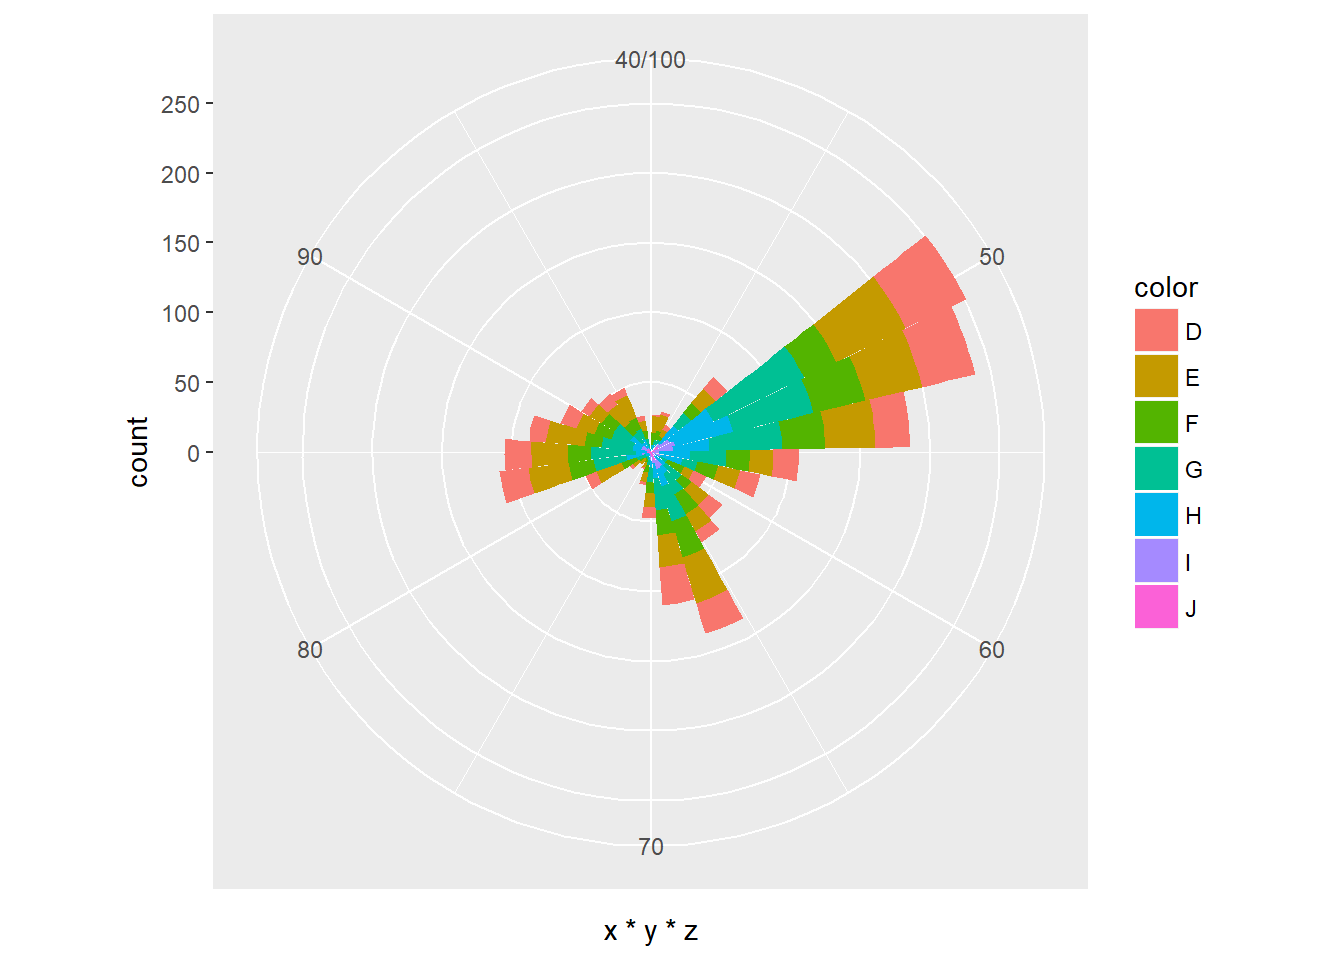
\includegraphics{osnoveR_files/figure-latex/unnamed-chunk-425-1.pdf}

\begin{Shaded}
\begin{Highlighting}[]
\CommentTok{# pogledajte kako sljedeći graf izgleda u "izvrnutom" }
\CommentTok{# a kako u polarnom koordinatnom sustavu}
\KeywordTok{ggplot}\NormalTok{(diamondsSample, }\KeywordTok{aes}\NormalTok{(}\DataTypeTok{x =}\NormalTok{ x}\OperatorTok{*}\NormalTok{y}\OperatorTok{*}\NormalTok{z, }\DataTypeTok{fill =}\NormalTok{ color)) }\OperatorTok{+}\StringTok{ }
\StringTok{  }\KeywordTok{geom_histogram}\NormalTok{(}\DataTypeTok{bins =} \DecValTok{30}\NormalTok{, }\DataTypeTok{na.rm =}\NormalTok{ T) }\OperatorTok{+}\StringTok{ }
\StringTok{  }\KeywordTok{xlim}\NormalTok{(}\DecValTok{40}\NormalTok{, }\DecValTok{100}\NormalTok{) }\OperatorTok{+}\StringTok{ }\KeywordTok{coord_flip}\NormalTok{() }
\end{Highlighting}
\end{Shaded}

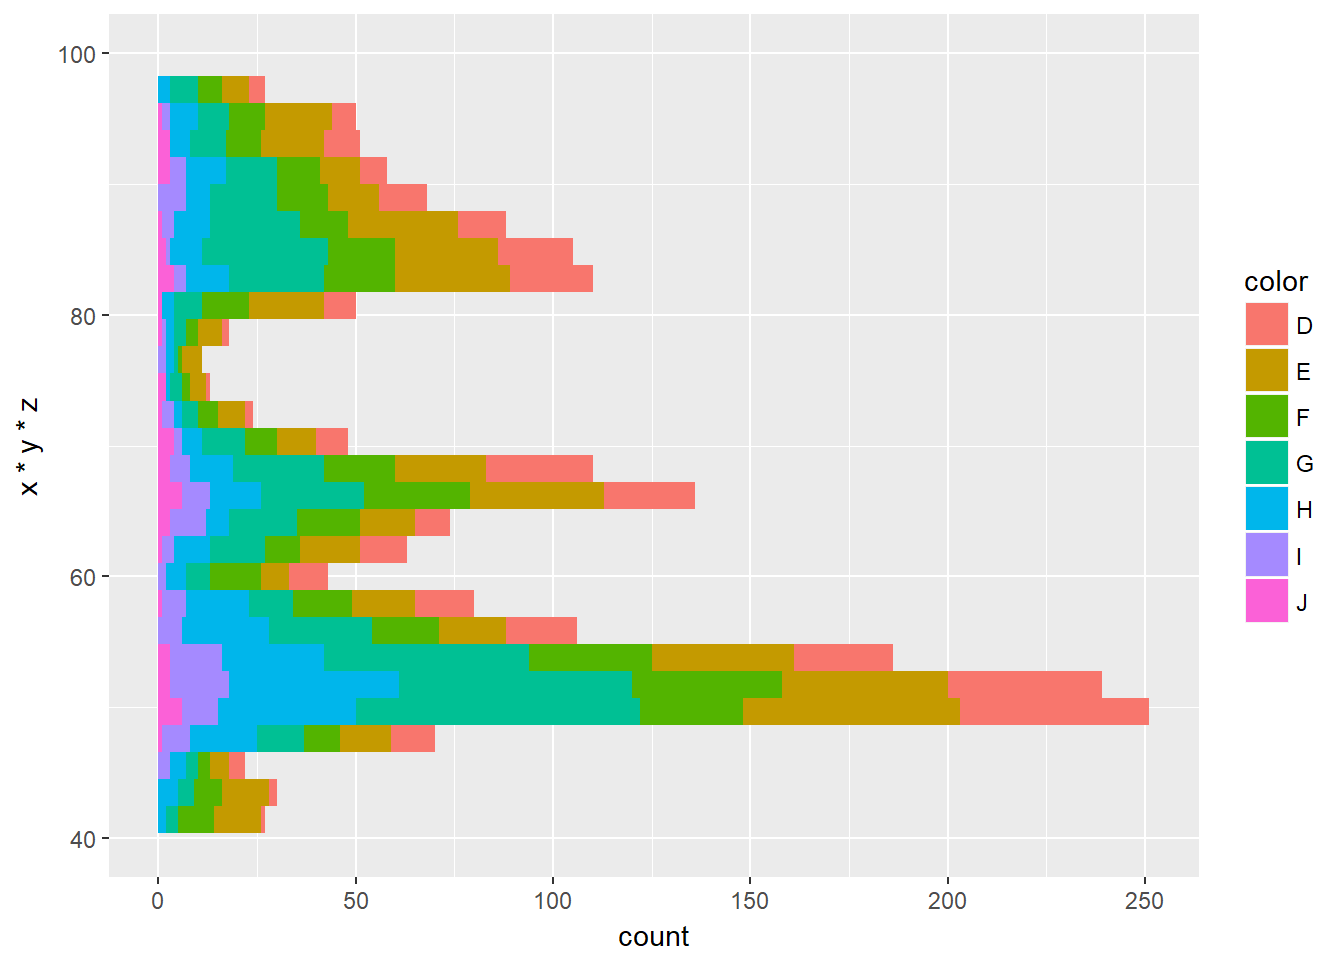
\includegraphics{osnoveR_files/figure-latex/unnamed-chunk-426-1.pdf}

\begin{center}\rule{0.5\linewidth}{\linethickness}\end{center}

Jedna od stvari koju je zgodno zapamtiti jest ta da \texttt{xlim} i
\texttt{ylim} parametri rade drugačije ovisno o tome da li ih koristimo
u aspektu skale ili koordinatnog sustava; limitiranje osi u aspektu
skale će ``izbaciti'' obzervacije koje su izvan zadanog intervala, što
može utjecati na izračun sumarnih statistika, krivulja zaglađivanja i
sl. S druge strane, limesi zadani u aspektu koordinatnog sustava
jednostavno će ``zumirati'' graf na odabrano područje a i dalje će sve
obzervacije ulaziti u izračune. I jedna i druga opcija su korisne,
ovisno o tome želimo li graf koji prikazuje sve relevantne podatke za
danu vizualizaciju ili graf koji predstavlja uvećani segment nekog
drugog grafa.

\begin{center}\rule{0.5\linewidth}{\linethickness}\end{center}

Konačno \textbf{aspekt teme grafa} nam omogućuje da utječemo na sve
vizualne aspekte grafa koji nisu povezani s podacima. To znači da možemo
birati boju i izgled pozadine, font i veličinu slova, margine,
poravnavanja i još niz drugih parametara grafa. Tema nam daje iznimno
detaljnu kontrolu nad izgledom grafa, a budući da se zapravo radi o
objektu (klase \texttt{theme}), temu grafa možemo pohraniti i
reciklirati za sve buduće vizualizacije. Isto tako, \texttt{ggplot2}
nudi niz već unaprijed pripremljenih tema za korištenje i daljnju
prilagodbu, a koje dohvaćamo uz skup pomoćnih funkcija od kojih su neke:

\begin{itemize}
\tightlist
\item
  \texttt{theme\_gray} - \emph{default}-na tema
\item
  \texttt{theme\_bw} - crno-bijele osi, pogodna za projiciranje grafova
\item
  \texttt{theme\_classic} - ``klasična'' tema slična onoj koju producira
  \texttt{plot} funkcija
\item
  \texttt{theme\_void} - ``prazna'' tema
\end{itemize}

\begin{center}\rule{0.5\linewidth}{\linethickness}\end{center}

\textbf{Zadatak 12.28 - odabir druge teme grafa}

\begin{Shaded}
\begin{Highlighting}[]
\CommentTok{# promijenite temu sljedećem grafu na `theme_classic`}
\KeywordTok{ggplot}\NormalTok{(diamondsSample, }\KeywordTok{aes}\NormalTok{(}\DataTypeTok{x =}\NormalTok{ x}\OperatorTok{*}\NormalTok{y}\OperatorTok{*}\NormalTok{z, }\DataTypeTok{fill =}\NormalTok{ color)) }\OperatorTok{+}\StringTok{ }
\StringTok{  }\KeywordTok{geom_histogram}\NormalTok{(}\DataTypeTok{bins =} \DecValTok{30}\NormalTok{, }\DataTypeTok{na.rm =}\NormalTok{ T) }\OperatorTok{+}\StringTok{ }
\StringTok{  }\KeywordTok{xlim}\NormalTok{(}\DecValTok{0}\NormalTok{, }\DecValTok{500}\NormalTok{) }
\end{Highlighting}
\end{Shaded}

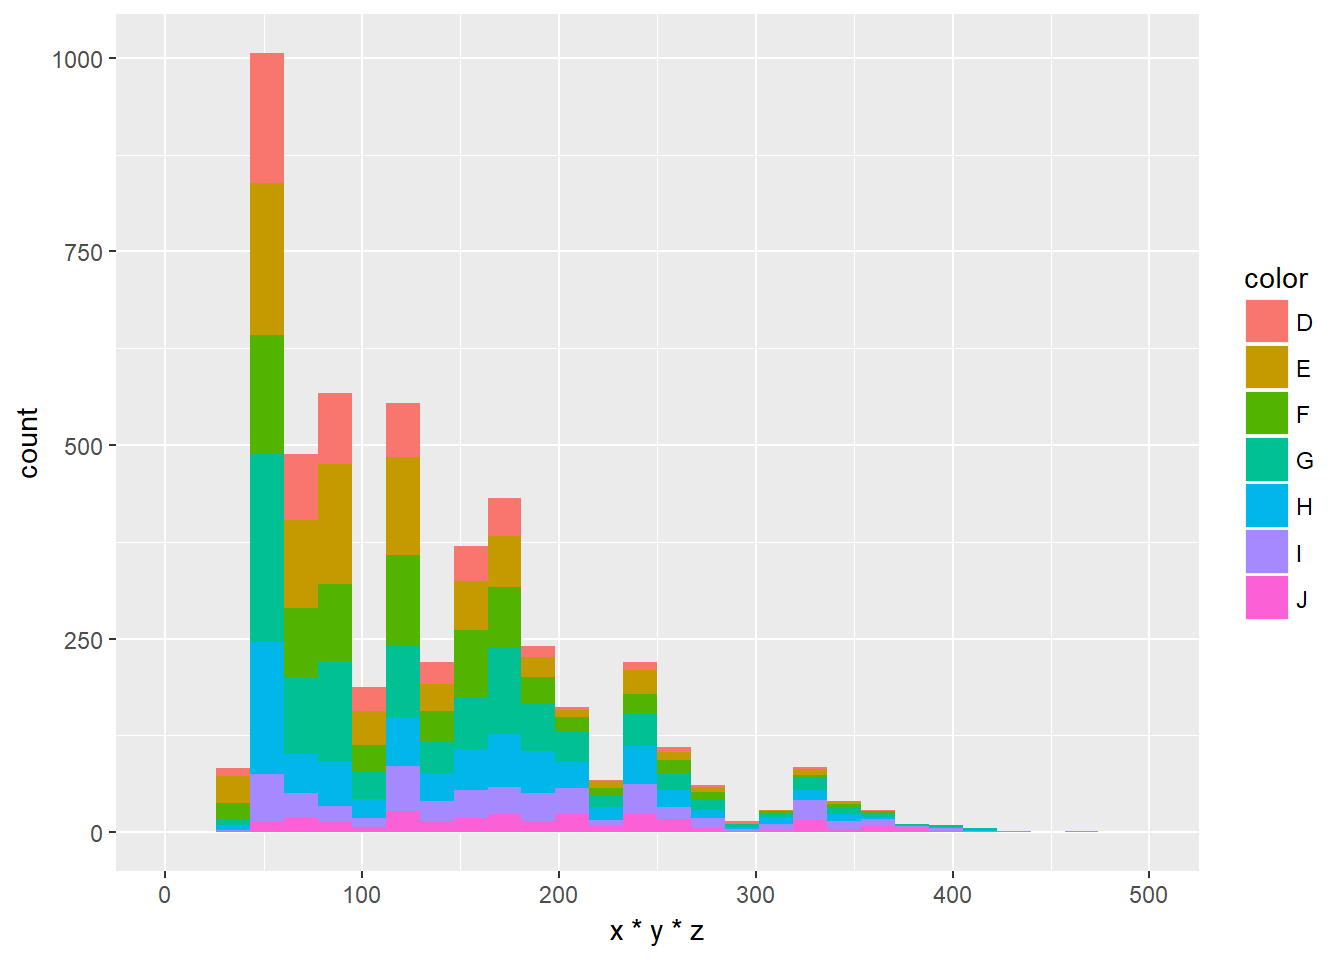
\includegraphics{osnoveR_files/figure-latex/unnamed-chunk-427-1.pdf}

\begin{Shaded}
\begin{Highlighting}[]
\CommentTok{# promijenite temu sljedećem grafu po izboru}
\KeywordTok{ggplot}\NormalTok{(diamondsSample, }\KeywordTok{aes}\NormalTok{(}\DataTypeTok{x =}\NormalTok{ x}\OperatorTok{*}\NormalTok{y}\OperatorTok{*}\NormalTok{z, }\DataTypeTok{fill =}\NormalTok{ color)) }\OperatorTok{+}\StringTok{ }
\StringTok{  }\KeywordTok{geom_histogram}\NormalTok{(}\DataTypeTok{bins =} \DecValTok{30}\NormalTok{, }\DataTypeTok{na.rm =}\NormalTok{ T) }\OperatorTok{+}\StringTok{ }
\StringTok{  }\KeywordTok{xlim}\NormalTok{(}\DecValTok{0}\NormalTok{, }\DecValTok{500}\NormalTok{) }\OperatorTok{+}\StringTok{ }\KeywordTok{theme_classic}\NormalTok{()}
\end{Highlighting}
\end{Shaded}

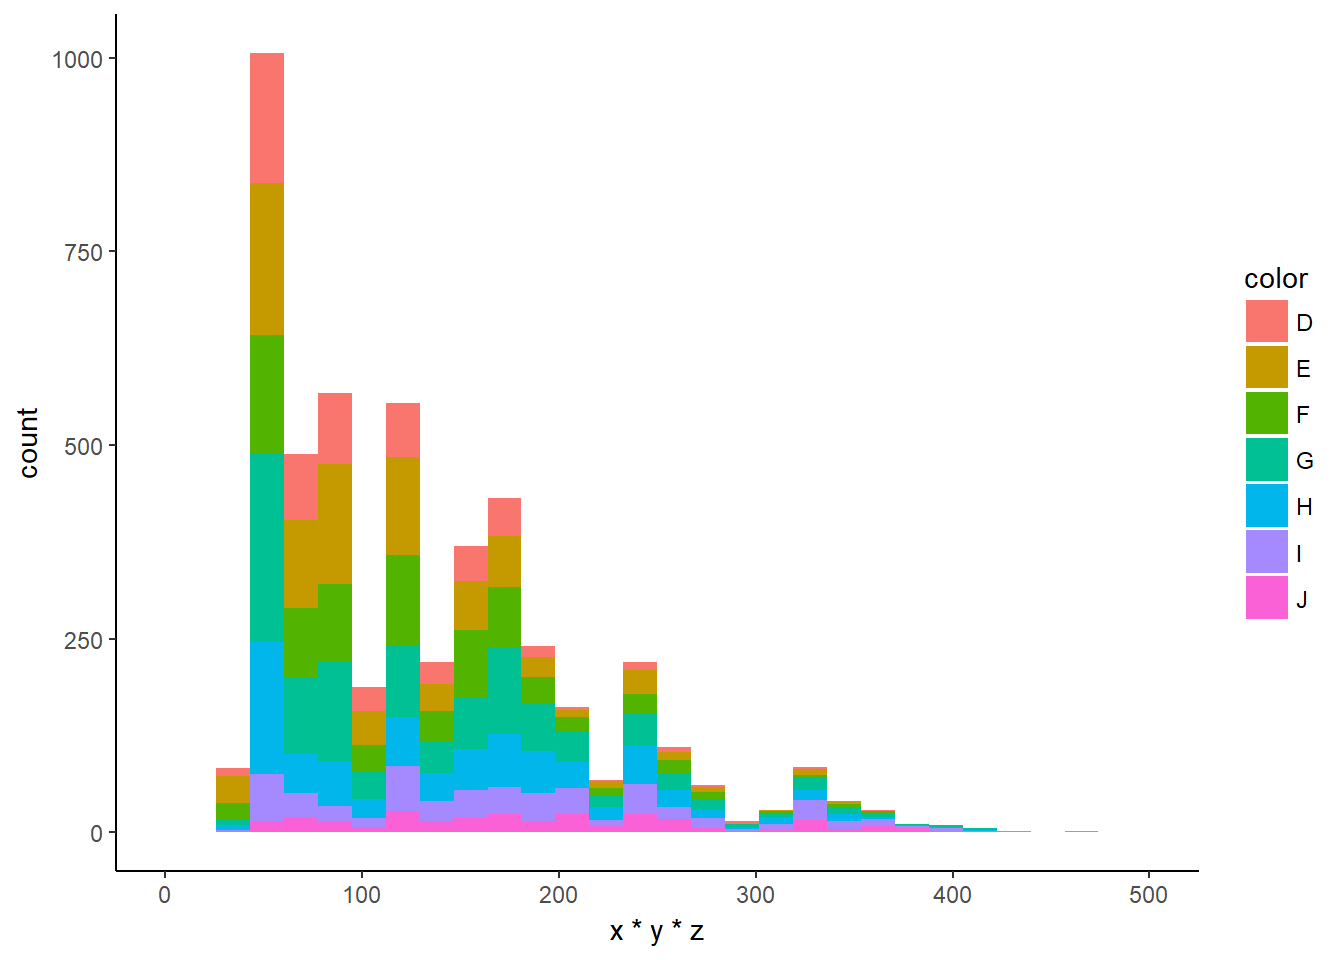
\includegraphics{osnoveR_files/figure-latex/unnamed-chunk-428-1.pdf}

Često želimo promijeniti samo neki od aspekata grafa koji nije vezan uz
podatke (npr. veličina ili orijentacija slova, izgled crtica na osima i
sl.). Za ove stvari koristimo funkciju \texttt{theme} koja sadrži vrlo
bogati niz parametara (pogledati dokumentaciju!). Neke od tih parametara
su tzv. ``elementi'' teme (npr. \texttt{element\_line},
\texttt{element\_text}) koje namještamo pozivom pripadne funkcije unutar
poziva funkcije \texttt{theme}, npr:

\begin{Shaded}
\begin{Highlighting}[]
\CommentTok{# mijenjamo izgled naziva grafa }
\CommentTok{# (za obitelj fontova preporučeno koristiti }
\CommentTok{#`serif`, `sans` ili `mono`)}
\NormalTok{... }\OperatorTok{+}\StringTok{ }\KeywordTok{theme}\NormalTok{( }\DataTypeTok{title =} \KeywordTok{element_text}\NormalTok{(}\DataTypeTok{family =} \StringTok{'serif'}\NormalTok{, }\DataTypeTok{face =} \StringTok{'bold.italic'}\NormalTok{))}
\end{Highlighting}
\end{Shaded}

\begin{center}\rule{0.5\linewidth}{\linethickness}\end{center}

\textbf{Zadatak 12.29 - izmjena elementa teme grafa}

\begin{Shaded}
\begin{Highlighting}[]
\CommentTok{# promijenite orijentaciju slova na x osi }
\CommentTok{# tako da budu pod kutem od 45 stupnjeva}
\KeywordTok{ggplot}\NormalTok{(diamondsSample, }\KeywordTok{aes}\NormalTok{(cut)) }\OperatorTok{+}\StringTok{ }\KeywordTok{geom_bar}\NormalTok{() }
\end{Highlighting}
\end{Shaded}

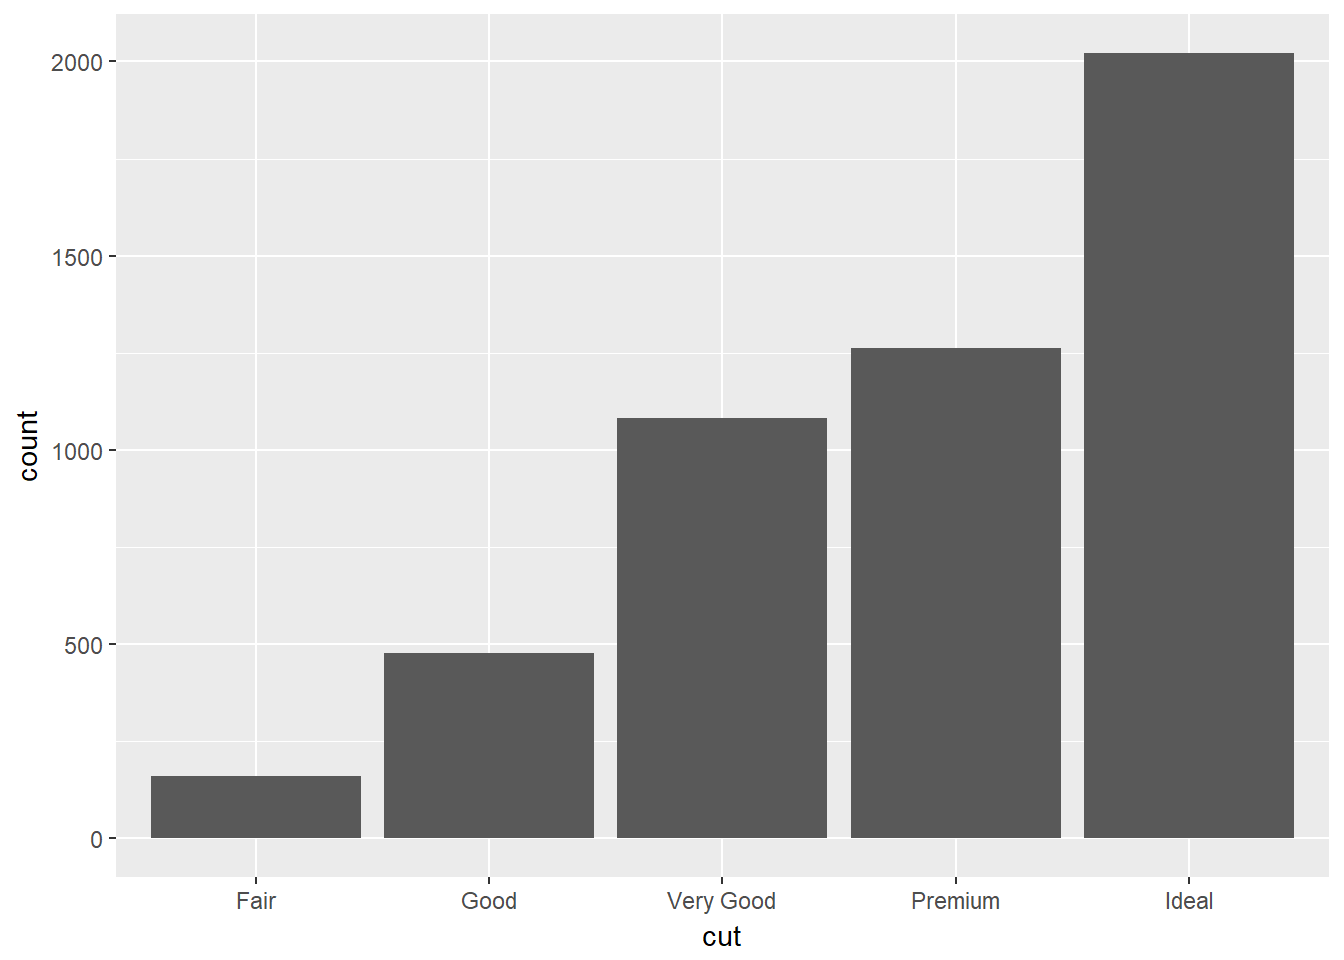
\includegraphics{osnoveR_files/figure-latex/unnamed-chunk-430-1.pdf}

\begin{Shaded}
\begin{Highlighting}[]
\KeywordTok{ggplot}\NormalTok{(diamondsSample, }\KeywordTok{aes}\NormalTok{(cut)) }\OperatorTok{+}\StringTok{ }\KeywordTok{geom_bar}\NormalTok{() }\OperatorTok{+}\StringTok{ }
\StringTok{  }\KeywordTok{theme}\NormalTok{(}\DataTypeTok{axis.text.x =} \KeywordTok{element_text}\NormalTok{(}\DataTypeTok{angle =} \DecValTok{45}\NormalTok{))}
\end{Highlighting}
\end{Shaded}

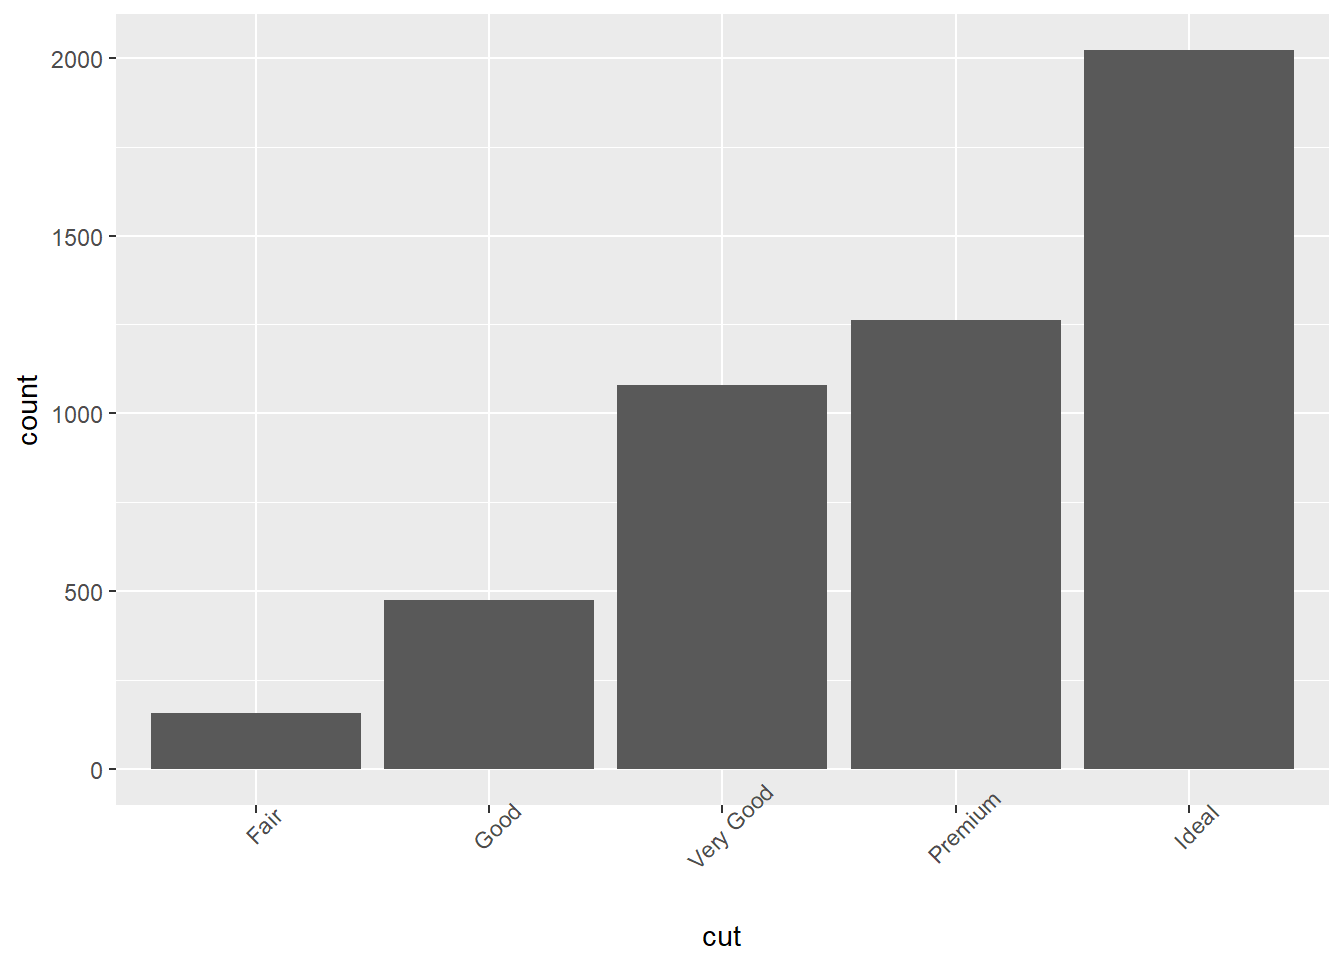
\includegraphics{osnoveR_files/figure-latex/unnamed-chunk-431-1.pdf}

\begin{center}\rule{0.5\linewidth}{\linethickness}\end{center}

\subsection{Uvjetni (facetirani)
grafovi}\label{uvjetni-facetirani-grafovi}

Već smo se upoznali sa estetikom grupiranja, koja prije vizualizacije
unutar skupa podataka radi podskupove po odabranoj varijabli te ih
shodno tome na adekvatan način vizualizira. Također smo naučili da
možemo raditi implicitna grupiranja uz pomoć estetika boje, oblika,
veličine i sl.

Ono što je zajedničko navedenim principima jest da se vizualno
razdvajanje u ovisnosti o nekoj varijabli provodi na istom grafu, tj.
koristimo se raznim estetikama kako bi prikazali nekoliko različitih
vizualizacijama u sklopu jedinstvenog grafa.

Uvjetni (facetirani) grafovi rade na istom principu, ali razdvajanje po
odabranoj varijabli (ili varijablama) radi se na način da se vizualizira
više grafova koji se onda prikazuju jedan pored drugoga. Rezultantni
grafovi prikazuju istu informaciju kao i estetika (implicitne ili
eksplicitne) grupe, ali je ovako nešto lakše proučiti svaki podgraf
zasebno.

Prije demonstracije kako radimo uvjetno grafove moramo objasniti pojam
tzv. ``notacije statističkih formula'' (\emph{statistical formula
notation}). Ova notacija se često koristi u R-u, pogotovo kod treniranja
raznih statističkih modela, a radi se zapravo o formalnoj notaciji
međuovisnosti varijabli nekog podatkovnog skupa zamišljenoj na način da
se može na što kraći i jednostavniji način zapisati i ugraditi u
programski kod.

Formule ćemo detaljnije obrađivati kasnije, a za sada ćemo pokazati samo
vrlo jednostavan primjer. Ako želimo zapisati ``y u ovisnosti o x-u'',
onda formula izgleda ovako:

\begin{Shaded}
\begin{Highlighting}[]
\NormalTok{y }\OperatorTok{~}\StringTok{ }\NormalTok{x          }\CommentTok{# znači "y u ovisnosti o x-u"}
\end{Highlighting}
\end{Shaded}

ovo možemo čitati i kao ``y kao funkcija od x'' ili - u slučaju
linearnih modela - ``y = ax + b''. Dakle, znak tilda
(\texttt{\textasciitilde{}}) zapravo znači ``u ovisnosti o''.

Prikažimo još neke jednostavnije oblike formula:

\begin{Shaded}
\begin{Highlighting}[]
\CommentTok{# z u ovisnost o x i y (plus ovdje nije aritmetičko zbrajanje!)}
\NormalTok{z }\OperatorTok{~}\StringTok{ }\NormalTok{x }\OperatorTok{+}\StringTok{ }\NormalTok{y  }

\CommentTok{# y u ovisnosti o "svim ostalim varijablama"}
\NormalTok{y }\OperatorTok{~}\StringTok{ }\NormalTok{. }

\CommentTok{# "sve ostale varijable" u ovisnosti o y}
\NormalTok{. }\OperatorTok{~}\StringTok{ }\NormalTok{y   }

\CommentTok{# tzv. "jednostrana" formula, "u ovisnosti o y"}
\OperatorTok{~}\StringTok{ }\NormalTok{y        }
\end{Highlighting}
\end{Shaded}

Zadnja dva primjera je malo teže matematički definirati no znaju se
koristiti u pozivima funkcija za različite svrhe, većinom zbog
jednostavnog zapisa i lake interpretacije.

Vratimo se sada na uvjetne grafove. Postoji dva osnovna načina stvaranja
uvjetnih grafova, a to je uz pomoć funkcija

\begin{itemize}
\tightlist
\item
  \texttt{facet\_grid} - za organizaciju ``podgrafova'' u mrežu tj.
  matricu
\item
  \texttt{facet\_wrap} - za organizaciju ``podgrafova'' u jedan ili više
  redaka
\end{itemize}

Funkciju \texttt{facet\_grid} koristimo kad podskupove radimo po jednoj
ili dvije kategorijske varijable. Rastavljanje po dvije varijable
prirodno radi ``matricu'', dok rastavljanje po jednoj će napraviti redak
ili stupac, što možemo kontrolirati formulom. Funkciju
\texttt{facet\_wrap} koristimo kada želimo rastaviti po jednoj
varijabli, ali ne želimo da svi budu u jednom stupcu ili retku već ih
želimo presložiti u više redaka (zato je i \emph{wrap}, slično kao
\emph{word wrap} u uređivaču teksta koji prenosi tekst u drugi red).

\begin{center}\rule{0.5\linewidth}{\linethickness}\end{center}

\textbf{Zadatak 12.30 - funkcija `facet\_grid'}

\begin{Shaded}
\begin{Highlighting}[]
\CommentTok{# reduciramo uzorak kako bi radili sa }
\CommentTok{# faktorima sa manjim brojem razina}
\NormalTok{diamondsSample }\OperatorTok\StringTok{ }
\StringTok{  }\KeywordTok{filter}\NormalTok{(color }\OperatorTok\StringTok{ }\KeywordTok{c}\NormalTok{(}\StringTok{"G"}\NormalTok{, }\StringTok{"H"}\NormalTok{, }\StringTok{"I"}\NormalTok{, }\StringTok{"J"}\NormalTok{),}
\NormalTok{         cut }\OperatorTok\StringTok{ }\KeywordTok{c}\NormalTok{(}\StringTok{"Very Good"}\NormalTok{, }
                    \StringTok{"Premium"}\NormalTok{, }\StringTok{"Ideal"}\NormalTok{)) ->}\StringTok{ }\NormalTok{diamondsSample2}

\CommentTok{# napravite uvjetni graf u ovisnosti o kombinaciji }
\CommentTok{# boje (`color`) i reza (`cut`)}
\CommentTok{# koristite funkciju `facet_grid` i }
\CommentTok{# formulu kao parametar}
\KeywordTok{ggplot}\NormalTok{(diamondsSample2, }\KeywordTok{aes}\NormalTok{(depth, }\DataTypeTok{fill =}\NormalTok{ clarity)) }\OperatorTok{+}\StringTok{ }
\StringTok{  }\KeywordTok{geom_histogram}\NormalTok{(}\DataTypeTok{bins =} \DecValTok{5}\NormalTok{,  }\DataTypeTok{position =} \StringTok{'dodge'}\NormalTok{)}
\end{Highlighting}
\end{Shaded}

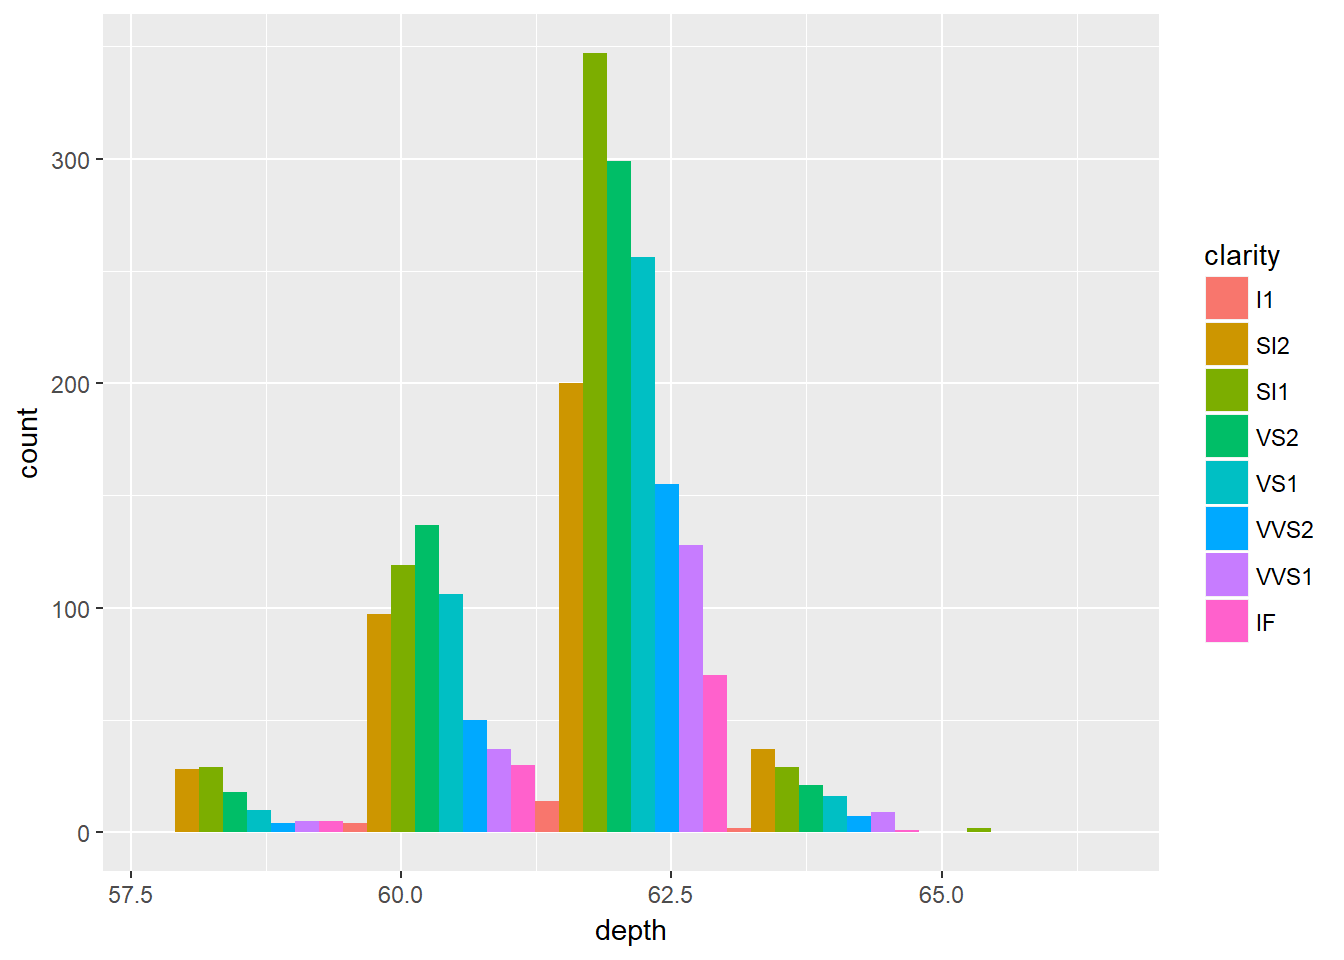
\includegraphics{osnoveR_files/figure-latex/unnamed-chunk-434-1.pdf}

\begin{Shaded}
\begin{Highlighting}[]
\KeywordTok{ggplot}\NormalTok{(diamondsSample2, }\KeywordTok{aes}\NormalTok{(depth, }\DataTypeTok{fill =}\NormalTok{ clarity)) }\OperatorTok{+}\StringTok{ }
\StringTok{  }\KeywordTok{geom_histogram}\NormalTok{(}\DataTypeTok{bins =} \DecValTok{5}\NormalTok{,  }\DataTypeTok{position =} \StringTok{'dodge'}\NormalTok{) }\OperatorTok{+}\StringTok{ }
\StringTok{  }\KeywordTok{facet_grid}\NormalTok{(color }\OperatorTok{~}\StringTok{ }\NormalTok{cut)}
\end{Highlighting}
\end{Shaded}

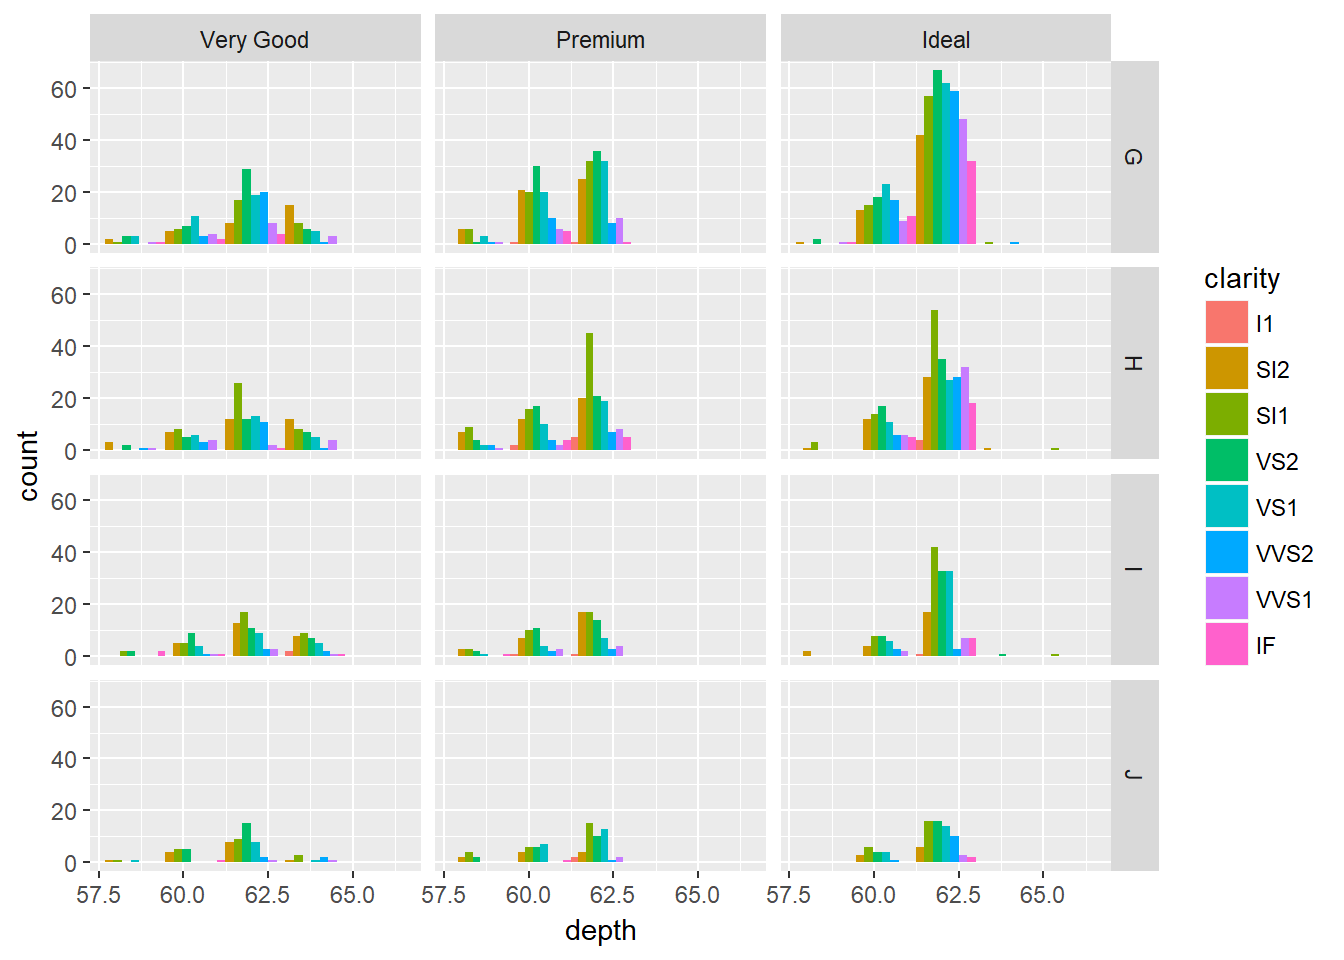
\includegraphics{osnoveR_files/figure-latex/unnamed-chunk-435-1.pdf}

\begin{center}\rule{0.5\linewidth}{\linethickness}\end{center}

\textbf{Zadatak 12.31 - funkcija `facet\_grid' (2)}

\begin{Shaded}
\begin{Highlighting}[]
\CommentTok{# ponovite postupak, ali sada rastavite samo po boji}
\CommentTok{# grafove organizirajte u stupac}
\CommentTok{# koristite funkciju `facet_grid` i notaciju formule sa točkom}
\KeywordTok{ggplot}\NormalTok{(diamondsSample2, }\KeywordTok{aes}\NormalTok{(depth, }\DataTypeTok{fill =}\NormalTok{ clarity)) }\OperatorTok{+}\StringTok{ }
\StringTok{  }\KeywordTok{geom_histogram}\NormalTok{(}\DataTypeTok{bins =} \DecValTok{5}\NormalTok{,  }\DataTypeTok{position =} \StringTok{'dodge'}\NormalTok{)}
\end{Highlighting}
\end{Shaded}

\begin{Shaded}
\begin{Highlighting}[]
\KeywordTok{ggplot}\NormalTok{(diamondsSample2, }\KeywordTok{aes}\NormalTok{(depth, }\DataTypeTok{fill =}\NormalTok{ clarity)) }\OperatorTok{+}\StringTok{ }
\StringTok{  }\KeywordTok{geom_histogram}\NormalTok{(}\DataTypeTok{bins =} \DecValTok{5}\NormalTok{,  }\DataTypeTok{position =} \StringTok{'dodge'}\NormalTok{) }\OperatorTok{+}\StringTok{ }\KeywordTok{facet_grid}\NormalTok{(color }\OperatorTok{~}\StringTok{ }\NormalTok{.)}
\end{Highlighting}
\end{Shaded}

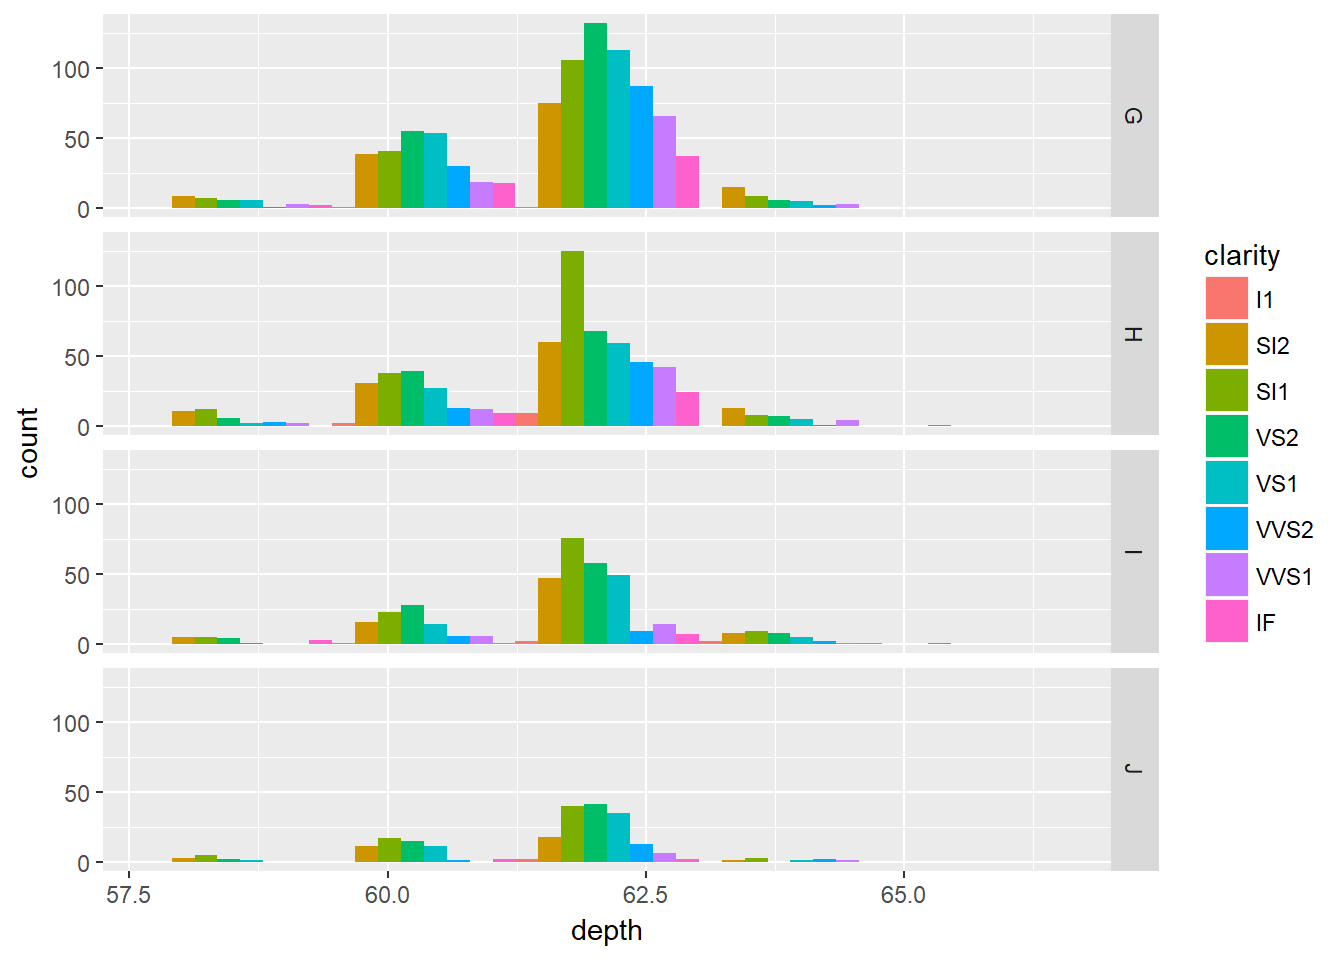
\includegraphics{osnoveR_files/figure-latex/unnamed-chunk-437-1.pdf}

\begin{center}\rule{0.5\linewidth}{\linethickness}\end{center}

Uočite jednu bitnu značajku uvjetnih grafova - koordinatne osi (tj.
skale) su poravnate. Naime, prije vizualizacije, \texttt{ggplot} prvo
``trenira'' skale na način da pronađe maksimalni raspon koji se onda
koristi kao zajednička značajka svih grafova. Ukoliko to ne želimo, može
određenu os (ili obje) učiniti slobodnom uz pomoć parametra
\texttt{scales} kojeg postavimo na \texttt{"free"} (za obje osi) ili
\texttt{"free\_x"} odnosno \texttt{"free\_y"} (ako želimo da samo jedna
os bude poravnata a druga ``slobodna'').

Pogledajmo još kako radi funkcija \texttt{facet\_wrap}:

\begin{center}\rule{0.5\linewidth}{\linethickness}\end{center}

\textbf{Zadatak 12.32 - funkcija `facet\_wrap'}

\begin{Shaded}
\begin{Highlighting}[]
\CommentTok{# razdvojite sljedeći graf u ovisnosti o prozirnosti (`clarity`)}
\CommentTok{# koristite funkciju `facet_wrap` i jednostranu formulu}
\KeywordTok{ggplot}\NormalTok{(diamondsSample2, }\KeywordTok{aes}\NormalTok{(x}\OperatorTok{*}\NormalTok{y}\OperatorTok{*}\NormalTok{z, price)) }\OperatorTok{+}\StringTok{ }\KeywordTok{geom_point}\NormalTok{() }
\end{Highlighting}
\end{Shaded}

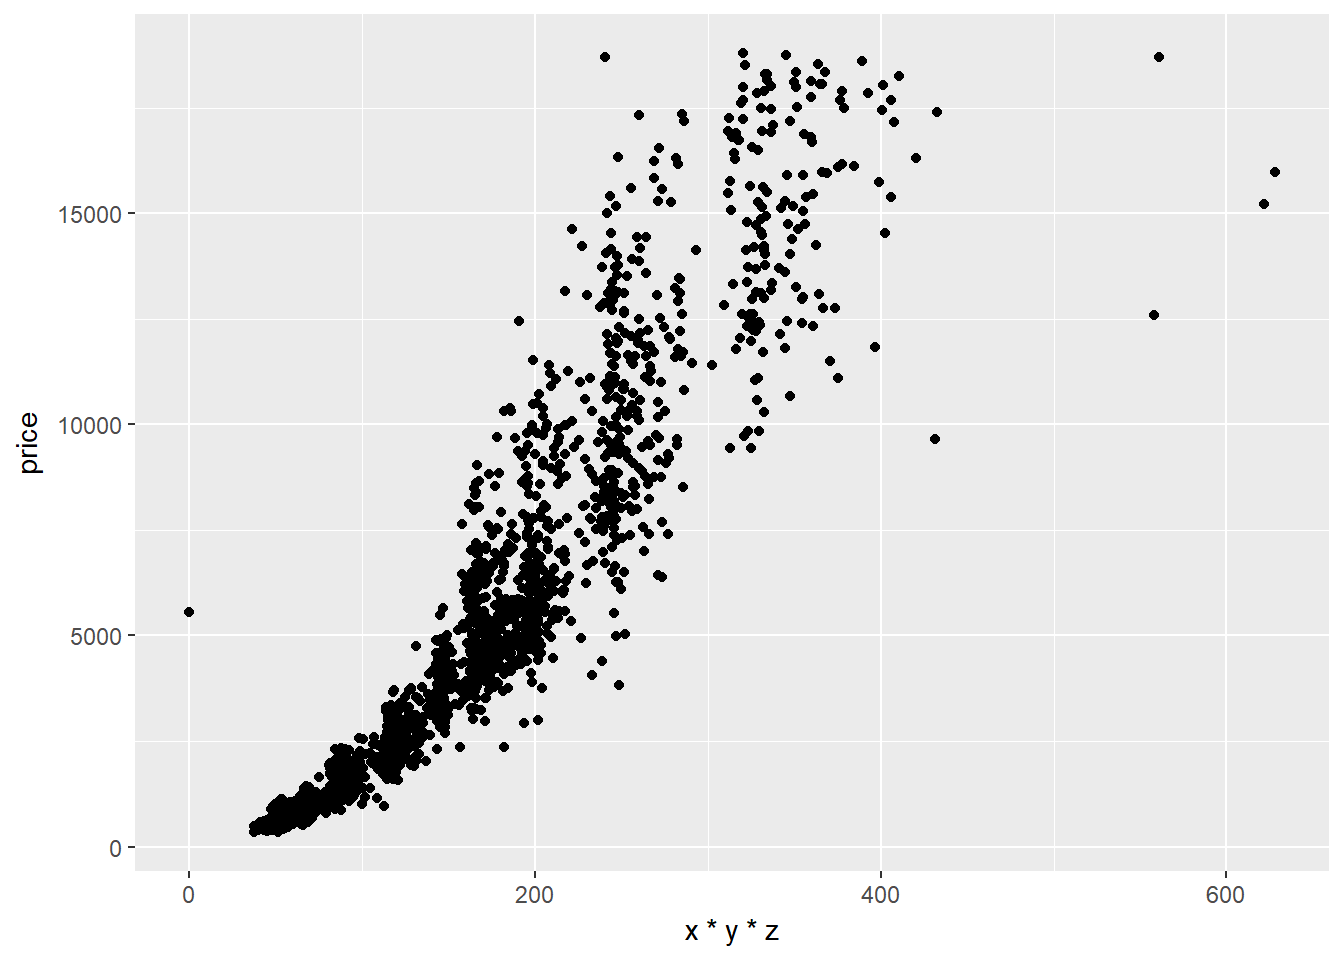
\includegraphics{osnoveR_files/figure-latex/unnamed-chunk-438-1.pdf}

\begin{Shaded}
\begin{Highlighting}[]
\KeywordTok{ggplot}\NormalTok{(diamondsSample2, }\KeywordTok{aes}\NormalTok{(x}\OperatorTok{*}\NormalTok{y}\OperatorTok{*}\NormalTok{z, price)) }\OperatorTok{+}\StringTok{ }
\StringTok{  }\KeywordTok{geom_point}\NormalTok{() }\OperatorTok{+}\StringTok{ }\KeywordTok{facet_wrap}\NormalTok{( }\OperatorTok{~}\StringTok{ }\NormalTok{clarity)}
\end{Highlighting}
\end{Shaded}

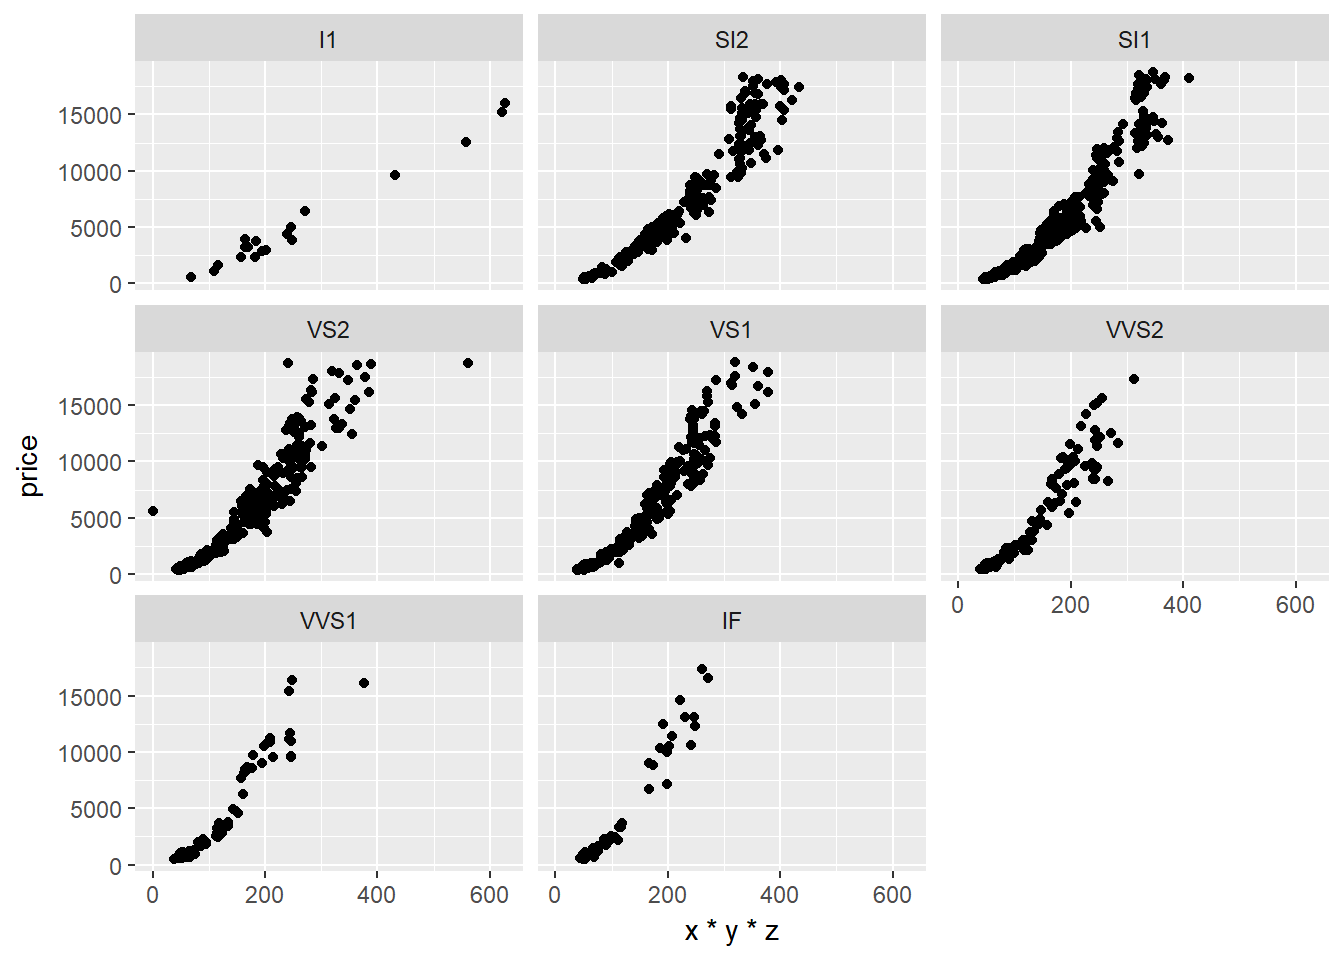
\includegraphics{osnoveR_files/figure-latex/unnamed-chunk-439-1.pdf}

\begin{center}\rule{0.5\linewidth}{\linethickness}\end{center}

Ovime završavamo priču o gramatičkoj geometriji, njezinim aspektima i
primjeni uz pomoć paketa \texttt{ggplot2}. Ovdje nisu ni približno
objašnjenje sve mogućnosti ovoga paketa, zbog čega se snažno preporučuje
dodatno čitanje dokumentacije i referenciranje na podsjetnik koji sadrži
niz geometrija i opcija za koje u ovim lekcijama nije bilo mjesta.
Također, ne treba zaboraviti na niz dodatnih paketa koji dodatno
proširuju mogućnosti paketa \texttt{ggplot2}, a koje bi trebalo
potražiti u ovisnosti o našim zahtjevima i željama glede vizualizacija
koje želimo stvoriti za naše projekte podatkovne analize. Za inspiraciju
zgodno je pogledati galeriju grafova i slika nastalih uz pomoć jezika R,
a koja je dostupna na ovoj poveznici .

\begin{center}\rule{0.5\linewidth}{\linethickness}\end{center}

\section{Grafovi u eksploratornoj analizi i
izvještavanju}\label{grafovi-u-eksploratornoj-analizi-i-izvjestavanju}

Za kraj možemo se kratko osvrnuti na razliku između grafova rađenih za
eksploratornu analizu podataka i onih koje koristimo u izvještajima, za
komunikaciju naših zaključaka drugim ljudima i prenošenje dobivenih
saznanja.

Kod eksploratorne analize podataka često je glavni cilj - kvantiteta.
Već je rečeno da se eksploratorna analiza svodi na traženje odgovora za
niz pitanja koje analitičar postavlja vezano uz podatke. Estetika ovdje
često nije bitna - glavno je da grafovi imaju dovoljno informacija da se
kod naknadnog pregledavanja može ono što je predočeno staviti u
odgovarajući kontekst. Analitičar će također često isprobavati različite
kombinacije estetika, geometrija i statistika. Ponekad je zgodno
koristiti i dodatne pakete koji omogućuju prikaz većeg broja varijabli
na istom grafu, npr. funkcija \texttt{ggpairs} paketa \texttt{GGally}:

\begin{Shaded}
\begin{Highlighting}[]
\CommentTok{#library(GGally)        #ako je potrebno}
\CommentTok{# uzimamo samo četiri stupca zbog jasnijeg prikaza}
\KeywordTok{ggpairs}\NormalTok{(}\DataTypeTok{data =}\NormalTok{ diamondsSample[,}\KeywordTok{c}\NormalTok{(}\DecValTok{1}\NormalTok{, }\DecValTok{2}\NormalTok{, }\DecValTok{5}\NormalTok{, }\DecValTok{7}\NormalTok{)])}
\end{Highlighting}
\end{Shaded}

\includegraphics{osnoveR_files/figure-latex/unnamed-chunk-440-1.pdf}

Eksploratorne grafove analitičar koristi radi predočavanja \textbf{samih
podataka}, kako bi potražio uzorke, prepoznao distribucije ili prirodna
grupiranja podataka ili uočio iskočne vrijednosti (tzv.
\emph{outlier}-e). Isto tako, eksploratorni grafovi se koriste za
predočavanje raznih \textbf{agregiranih statistika}. Ukoliko se radi o
prediktivnoj analizi podataka, tj. cilj analize jest razviti metodu
predviđanja nekih varijabli na osnovu drugih varijabli podatkovnog
skupa, analitičar će često u tijeku eksploratorne analize stvoriti
nekoliko jednostavnijih prediktivnih modela koje će onda vizualizirati
na grafu kako bi mogao slikom predočiti učinkovitost modela te na osnovu
uočenih nedostataka razviti strategiju za daljnje korake analize.

Kod izvještavanja s druge strane ključna je kvaliteta grafa u smislu
jasnog i preglednog predstavljanja informacije. Graf mora jasno
komunicirati informacije koje su njime predočene, uz pažljivo odabrana
objašnjenja i pomno odabrano korištenje tzv. \textbf{metapodataka}, tj.
dodatnog teksta i anotacija. Za stvaranje izvještajnih grafova
preporučuje se koristiti dodatne \texttt{geom\_text} slojeve za
tekstualnim oznakama na odgovarajućim područjima grafa gdje one mogu
najviše doprinijeti, a također i kreativno korištenje
\texttt{geom\_point}, \texttt{geom\_hline}, \texttt{geom\_vline},
\texttt{geom\_rect} i sličnih geometrijskih slojeva koji će dodatno
pojasniti određene segmente grafa. Isto tako, preporučuje se unaprijed
pripremiti temu koju ćemo onda konzistentno primjenjivati na sve
grafove.

U velikom broju slučajeva grafovi u izvještajima su zapravo probrani i
``uljepšani'' grafovi dobiveni tijekom eksploratorne analize. No
analitičar bi trebao posebnu pažnju posvetiti činjenici da se grafovi u
izvještajima često rade za publiku koja je daleko manje upoznata sa
podatkovnim skupom i raznim detaljnim saznanjima koje je analitičar
dobio tijekom eksploratorne analize. Izvještajni grafovi stoga moraju
biti orijentirani krajnjem korisniku, te s tim ciljem i pažljivo
dizajnirani. Zbog toga se preporučuje da svi elementi grafa -
uključujući i naslov, legende i sl. budu orijentirani komunikaciji
informacije i razjašnjenju što graf prikazuje, a što je u skladu sa
zaključcima koje publikacija iznosi.

Konačno, ponekad želimo zbog štednje prostora unutar jedne slike staviti
više različitih grafova. Ovo obično radimo uz pomoć više zasebnih slika
koje slažemo unutar sučelja kojeg koristimo za pisanje publikacije čiji
su dio navedeni grafovi, no možemo i unaprijed pripremiti grafove uz
pomoć paketa \texttt{gridExtra}. Između ostalog, ovaj paket nudi
funkciju \texttt{grid.arrange} uz pomoć koje grafove slažemo u matricu s
odabranim brojem redaka i stupaca.

\begin{Shaded}
\begin{Highlighting}[]
\CommentTok{#library(gridExtra)    # ukoliko je potrebno}

\CommentTok{# grafove koje slažem u matricu pohranjujem u varijable}
\NormalTok{g1 <-}\StringTok{ }\KeywordTok{ggplot}\NormalTok{(diamondsSample, }\KeywordTok{aes}\NormalTok{(x}\OperatorTok{*}\NormalTok{y}\OperatorTok{*}\NormalTok{z, price, }\DataTypeTok{color =}\NormalTok{ color)) }\OperatorTok{+}\StringTok{ }
\StringTok{  }\KeywordTok{geom_point}\NormalTok{(}\DataTypeTok{alpha =} \FloatTok{0.6}\NormalTok{)}

\NormalTok{g2 <-}\StringTok{ }\KeywordTok{ggplot}\NormalTok{(diamondsSample, }\KeywordTok{aes}\NormalTok{(}\DataTypeTok{x =}\NormalTok{ x}\OperatorTok{*}\NormalTok{y}\OperatorTok{*}\NormalTok{z, }\DataTypeTok{fill =}\NormalTok{ color)) }\OperatorTok{+}\StringTok{ }
\StringTok{  }\KeywordTok{geom_histogram}\NormalTok{(}\DataTypeTok{bins =} \DecValTok{30}\NormalTok{, }\DataTypeTok{na.rm =}\NormalTok{ T) }\OperatorTok{+}\StringTok{ }
\StringTok{  }\KeywordTok{scale_fill_brewer}\NormalTok{(}\DataTypeTok{palette =} \StringTok{"Greens"}\NormalTok{)}

\NormalTok{g3 <-}\StringTok{ }\KeywordTok{ggplot}\NormalTok{(diamondsSample, }\KeywordTok{aes}\NormalTok{(}\DataTypeTok{x =}\NormalTok{ cut)) }\OperatorTok{+}\StringTok{ }
\StringTok{  }\KeywordTok{geom_bar}\NormalTok{(}\DataTypeTok{fill =} \StringTok{"blue"}\NormalTok{, }\DataTypeTok{alpha =} \FloatTok{0.5}\NormalTok{)}

\NormalTok{g4 <-}\StringTok{ }\KeywordTok{ggplot}\NormalTok{(diamondsSample, }\KeywordTok{aes}\NormalTok{(}\DataTypeTok{x =}\NormalTok{ color, }\DataTypeTok{fill =}\NormalTok{ clarity)) }\OperatorTok{+}\StringTok{ }
\StringTok{  }\KeywordTok{geom_bar}\NormalTok{() }\OperatorTok{+}\StringTok{ }\KeywordTok{coord_polar}\NormalTok{()}

\CommentTok{# pozivam funkciju `grid.arrange`}
\KeywordTok{grid.arrange}\NormalTok{(g1, g2, g3, g4, }\DataTypeTok{nrow =} \DecValTok{2}\NormalTok{, }\DataTypeTok{ncol =} \DecValTok{2}\NormalTok{)}
\end{Highlighting}
\end{Shaded}

\includegraphics{osnoveR_files/figure-latex/unnamed-chunk-441-1.pdf}

\begin{center}\rule{0.5\linewidth}{\linethickness}\end{center}

\section*{Zadaci za vježbu}\label{zadaci-za-vjezbu-10}
\addcontentsline{toc}{section}{Zadaci za vježbu}

\begin{enumerate}
\def\labelenumi{\arabic{enumi}.}
\tightlist
\item
  Učitajte i proučite podatkovni skup \texttt{diamonds} koji dolazi
  zajedno s paketom \texttt{ggplot2}.
\end{enumerate}

\begin{enumerate}
\def\labelenumi{\alph{enumi})}
\item
  Prikažite raspodjelu cijene dijamanata uz pomoć dva grafa - histograma
  i tzv. \emph{frekvencijskih poligona} (funkcija
  \texttt{geom\_freqpoly})). Cijene podijelite u 10 ladica.
\item
  Grafovima iz a) dodajte ``čistoću'' dijamanta (stupac
  \texttt{clarity}) koji ćete postaviti na \texttt{fill} estetiku
  (histogram) odnosno \texttt{color} estetiku (frekvencijski poligoni).
  Koju razliku između grafova uočavate obzirom na \emph{default}-ni
  aspekt pozicije?
\end{enumerate}

\begin{enumerate}
\def\labelenumi{\arabic{enumi}.}
\setcounter{enumi}{1}
\tightlist
\item
  Učitajte i proučite podatkovni skup \texttt{mpg}. Pokušajte
  rekonstruirati sljedeće grafove. Nepoznate geometrije identificirajte
  uz pomoć podsjetnika.
\end{enumerate}

\includegraphics{osnoveR_files/figure-latex/unnamed-chunk-442-1.pdf}

\begin{center}\rule{0.5\linewidth}{\linethickness}\end{center}

\includegraphics{osnoveR_files/figure-latex/unnamed-chunk-443-1.pdf}

\begin{center}\rule{0.5\linewidth}{\linethickness}\end{center}

\includegraphics{osnoveR_files/figure-latex/unnamed-chunk-444-1.pdf}

\begin{center}\rule{0.5\linewidth}{\linethickness}\end{center}

\begin{enumerate}
\def\labelenumi{\arabic{enumi}.}
\setcounter{enumi}{2}
\tightlist
\item
  Uz pomoć funkcija skaliranja na sljedećem grafu:
\end{enumerate}

\begin{enumerate}
\def\labelenumi{\alph{enumi})}
\tightlist
\item
  os x nazovite \texttt{"broj\ cilindara"}
\item
  os y nazovite \texttt{"ukupno"} i povećajte raspon do 100
\item
  legendu za godine nazovite \texttt{"godina"}
\item
  za boju pravokutnika odaberite paletu \texttt{"Dark2"}
\end{enumerate}

\begin{Shaded}
\begin{Highlighting}[]
\KeywordTok{ggplot}\NormalTok{(mpg, }\KeywordTok{aes}\NormalTok{(}\DataTypeTok{x =} \KeywordTok{as.factor}\NormalTok{(cyl), }
                \DataTypeTok{fill =} \KeywordTok{as.factor}\NormalTok{(year))) }\OperatorTok{+}\StringTok{ }\KeywordTok{geom_bar}\NormalTok{()}
\end{Highlighting}
\end{Shaded}

\includegraphics{osnoveR_files/figure-latex/unnamed-chunk-445-1.pdf}

\begin{enumerate}
\def\labelenumi{\arabic{enumi}.}
\setcounter{enumi}{3}
\tightlist
\item
  Promijenite temu sljedećeg grafa na sljedeći način:

  \begin{enumerate}
  \def\labelenumii{\alph{enumii})}
  \tightlist
  \item
    prilagodite prikaz projekciji na platno
  \item
    okrenite nazive na x osi vertikalno
  \end{enumerate}
\end{enumerate}

\begin{Shaded}
\begin{Highlighting}[]
\KeywordTok{ggplot}\NormalTok{(mpg, }\KeywordTok{aes}\NormalTok{(}\DataTypeTok{x =} \KeywordTok{as.factor}\NormalTok{(trans), }\DataTypeTok{y =}\NormalTok{ displ)) }\OperatorTok{+}\StringTok{ }
\StringTok{  }\KeywordTok{geom_boxplot}\NormalTok{() }
\end{Highlighting}
\end{Shaded}

\includegraphics{osnoveR_files/figure-latex/unnamed-chunk-446-1.pdf}

\begin{enumerate}
\def\labelenumi{\arabic{enumi}.}
\setcounter{enumi}{4}
\tightlist
\item
  Sljedeći graf prikazuje histogram potrošnje na autocesti pri čemu boja
  pravokutnika odražava broj cilindara. Pokušajte poboljšati
  interpretabilnost grafa tako da estetiku boje zamijenite prikazom više
  grafova uvjetovanih brojem cilindara. Grafove organizirajte u matricu
  2 x 2.
\end{enumerate}

\begin{Shaded}
\begin{Highlighting}[]
\KeywordTok{ggplot}\NormalTok{(mpg, }\KeywordTok{aes}\NormalTok{(hwy, }\DataTypeTok{fill =} \KeywordTok{as.factor}\NormalTok{(cyl))) }\OperatorTok{+}\StringTok{ }
\StringTok{  }\KeywordTok{geom_histogram}\NormalTok{(}\DataTypeTok{bins =} \DecValTok{10}\NormalTok{, }\DataTypeTok{position =} \StringTok{"dodge"}\NormalTok{)}
\end{Highlighting}
\end{Shaded}

\includegraphics{osnoveR_files/figure-latex/unnamed-chunk-447-1.pdf}

\begin{enumerate}
\def\labelenumi{\arabic{enumi}.}
\setcounter{enumi}{5}
\tightlist
\item
  Pretpostavimo da imamo sljedeći podatkovni okvir:
\end{enumerate}

\begin{Shaded}
\begin{Highlighting}[]
\NormalTok{prodaja <-}\StringTok{ }\KeywordTok{data.frame}\NormalTok{(}\DataTypeTok{mjesec =} \DecValTok{1}\OperatorTok{:}\DecValTok{12}\NormalTok{,}
          \DataTypeTok{ukupno =} \KeywordTok{c}\NormalTok{(}\DecValTok{10000}\NormalTok{, }\DecValTok{5000}\NormalTok{, }\DecValTok{12000}\NormalTok{, }\DecValTok{3000}\NormalTok{, }\DecValTok{5000}\NormalTok{, }\DecValTok{7000}\NormalTok{, }
                   \DecValTok{10000}\NormalTok{, }\DecValTok{2000}\NormalTok{, }\DecValTok{4000}\NormalTok{, }\DecValTok{8000}\NormalTok{, }\DecValTok{11000}\NormalTok{, }\DecValTok{14000}\NormalTok{))}
\end{Highlighting}
\end{Shaded}

i da ga želimo predočiti stupčastim grafom (engl. \emph{bar chart}), no
funkcija \texttt{geom\_bar} po \emph{default}-u radi sa samo jednom
varijablom za koju računa sumarne statistike. Kako riješiti ovaj
problem? Predložite rješenje i stvorite odgovarajući stupčasti graf.

\begin{center}\rule{0.5\linewidth}{\linethickness}\end{center}

{Programirajmo u R-u} by Damir Pintar is licensed under a Creative
Commons Attribution-NonCommercial-NoDerivatives 4.0 International
License.Based on a work at https://ratnip.github.io/FER\_OPJR/

\part{Statistika i strojno učenje u jeziku
R}\label{part-statistika-i-strojno-ucenje-u-jeziku-r}

\chapter{Statističko programiranje, razdiobe i
simulacije}\label{razdiobe}

R se između ostalog definira kao jezik za ``statističko programiranje''
što znači da je jedna od njegovih osnovnih funkcija omogućiti provođenje
statističkih analiza. Za razliku od drugih programskih jezika, za R se
često kaže da je stvoren ``od statističara, za statističare'', što znači
da usprkos činjenici da je R kao jezik uvelike napredovao i evoluirao od
svojih početaka kao izvedenice jezika S, statistika je i dalje u srži
samog jezika a R kao takav sadrži iznimno bogatu podršku orijentiranu
upravo statističarima i njihovim potrebama.

Cilj lekcije koja slijedi nije naučiti čitatelja statistiku. Budući da
se radi o kompleksnom i relativno zahtjevnom znanstvenom polju za bilo
kakav svrsishodan pregled trebalo bi daleko više prostora od onoga koji
imamo ovdje na raspolaganju. Ideja lekcije jest primarno prikazati
funkcije rada sa razdiobama, objasniti osnove provedbe simulacija te
objasniti neke osnovne metode deskriptivne i inferencijalne statistike
uz naglasak na njihovo provođenje kroz programski jezik R. Čitatelji
koji nisu upoznati sa statistikom mogu lekciju koristiti kao prvi korak
prema upoznavanju svijeta statistike, dok oni koji upravljaju znanjem
barem osnovnih statističkih metoda mogu saznati kako neke poslove (koje
su možda obavljali uz pomoć nekih drugih alata) mogu izvršavati
programski uz pomoć podrške koju nudi jezik R.

Kao puno opsežniji uvod u statistiku snažno preporučujemo knjigu
``OpenIntro Statistics'' \citep{diez2015openintro}. Važno je napomenuti
da knjiga ima i svoj prateći CRAN paket, zvan `openintro', koji
omogućuje paralelno čitanje knjige i rješavanje zadanih problema
direktno u R-u na istim podatkovnim skupovima koji se referenciraju u
knjizi.

\begin{center}\rule{0.5\linewidth}{\linethickness}\end{center}

\section{Rad sa razdiobama vjerojatnosti u jeziku
R}\label{rad-sa-razdiobama-vjerojatnosti-u-jeziku-r}

U ovom dijelu lekcije prikazat ćemo podršku jezika R za rad sa
različitim razdiobama vjerojatnosti. Važno je naglasiti da se ovdje
nećemo baviti temeljitim pregledom teorije vezanim uz pojmove razdiobe
vjerojatnosti diskretne i kontinuirane slučajne varijable (već spomenuti
izvor ``OpenIntro Statistics'' može pružiti vrlo kvalitetan uvod ove
tematike). Cilj lekcije koja slijedi primarno je prikazati što jezik R -
ili konkretnije paket \texttt{stats} - nudi kao podršku za lak i
učinkovit rad sa razdiobama.

Pojam \emph{razdiobe vjerojatnosti} predstavlja funkciju koja opisuje
vjerojatnost pojave nekog slučajnog događaja. Tako kod bacanja novčića
imamo dva moguća ishoda - ``pismo'' ili ``glava'', a ako je novčić
regularan vjerojatnost pojedinog ishoda jest 0.5, tj. 50\%. Zbroj
brojeva kod bacanja dvije kockice može biti od 2 do 12, pri čemu svi
ishodi nemaju istu vjerojatnost; npr. broj 7 ima najveću vjerojatnost
(17\%) dok 2 i 12 imaju najmanju (samo 3\%).

Možemo razlikovati \emph{diskretne} i \emph{kontinuirane} razdiobe
vjerojatnosti. Najveća razlika među njima jest ta što kod kontinuiranih
razdiobi slučajna varijabla koju opisuju teoretski može poprimiti jednu
od beskonačnog broja mogućih vrijednosti tako da ne možemo pričati o
vjerojatnosti konkretnog ishoda; zbog toga kod kontinuiranih razdioba
pričamo o vjerojatnosti da varijabla bude \emph{manja ili jednaka} nekoj
vrijednosti.

Postoji veliki broj razdioba vjerojatnosti koje nam mogu poslužiti u
različitim scenarijima. \emph{Binomna razdioba} opisuje vjerojatnost
uočavanja nekog događaja u eksperimentu kojeg ponavljamo određeni broj
puta (npr. vjerojatnost da u 10 bacanja novčića dobijemo pismo 8 puta).
\emph{Geometrijska razdioba} opisuje vjerojatnost broja ponavljanja
nekog eksperimenta dok ne dočekamo neki ishod ishoda (npr. vjerojatnost
da se prvo ``pismo'' pojavi tek u petom bacanju novčića). Konačno, možda
najpoznatija razdioba je \emph{Gaussova} ili \emph{normalna razdioba}
koja se često pojavljuje u prirodi i koju statističari vrlo često
koriste za potrebe inferencijalne statistike.

Poznavanje funkcija za rad sa različitim razdiobama može nam uvelike
pomoći u različitim scenarijima. Na sreću, ne moramo poznavati veliki
broj razdiobi niti u detalje učiti matematičku podlogu svake od njih.
Dovoljno je početi sa nekoliko osnovnih razdiobi (npr. normalna i
uniformna) a potom polako širiti znanje o ostalim razdiobama kada se
suočimo sa problemima gdje se one mogu pokazati korisnima. Jezik R nam
ovdje prilično pomaže budući da koristi jedinstven predložak za podršku
svim funkcijama razdiobe koje imamo na raspolaganju tako da kad naučimo
upravljati podrškom za jednu razdiobu imamo kvalitetnu podlogu za
korištenje bilo koje druge razdiobe, jednom kad se upoznamo s njenim
specifičnostima i scenarijima uporabe.

Broj razdiobi koje imaju ugrađenu podršku u jeziku R je prilično velik.
Popis razdiobi koje imamo na raspolaganju - ne računajući dodatne CRAN
pakete! - možemo dobiti naredbom:

\begin{Shaded}
\begin{Highlighting}[]
\KeywordTok{help}\NormalTok{(Distributions)}
\end{Highlighting}
\end{Shaded}

\begin{center}\rule{0.5\linewidth}{\linethickness}\end{center}

U pravilu za svaku raspodjelu imamo na raspolaganju četiri funkcije koje
prate isti uzorak imenovanja - funkcije slijede naziv distribucije (npr.
\texttt{norm} za normalnu razdiobu, \texttt{unif} za uniformnu,
\texttt{binom} za binomnu i sl.). Ovom nazivu daje se prefiks od jednog
slova kako slijedi:

\begin{itemize}
\tightlist
\item
  \texttt{d} - za funkciju gustoće razdiobe
\item
  \texttt{p} - za funkciju razdiobe (kumulativna funkcija)
\item
  \texttt{q} - za funkciju kvantila (inverz od funkcije razdiobe)
\item
  \texttt{r} - za nasumično generiranje jedne ili više varijabli iz
  odabrane razdiobe
\end{itemize}

Svaka od ovih funkcija prima parametre specifične za njenu
funkcionalnost (tako funkcija za nasumični odabir varijabli iz razdiobe
prima parametar \texttt{n} koji joj daje informaciju broju slučajnih
varijabli koje želimo generirati) te parametre specifične za tu razdiobu
(tako sve funkcije za normalnu razdiobu primaju aritmetičku sredinu i
standardnu devijaciju tj. parametre \texttt{mean} i \texttt{sd},
geometrijska razdioba traži vektor vjerojatnosti \texttt{prob}, a
Poissonova parametar \texttt{lambda}).

U nastavku ćemo se (uglavnom) usredotočiti na normalnu (Gaussovu)
razdiobu, budući da se radi o poznatoj, sveprisutnoj razdiobi s koju
ćemo i najčešće susretati u praksi. No bitno je napomenuti da će većina
stvari prikazanih na normalnoj razdiobi biti primjenjiva i na druge
razdiobe, obzirom na činjenicu da su pripadajuće \emph{R}-ove funkcije
za rad sa razdiobama dizajnirane prema istom, gore prikazanom predlošku.
Za normalnu razdiobu tako imamo funkcije \texttt{dnorm}, \texttt{pnorm},
\texttt{qnorm} i \texttt{rnorm}. Potonju smo već upoznali u primjerima u
kojima smo generirali vektor slučajnih vrijednosti iz normalne razdiobe.
Pogledajmo u nastavku kako nam i preostale tri mogu poslužiti u praksi.

Već smo rekli da funkcije normalne razdiobe primaju parametre
\texttt{mean} i \texttt{sd} kojima definiramo aritmetičku sredinu i
standardnu devijaciju normalne razdiobe s kojom želimo raditi. Ukoliko
te parametre ne navedemo pretpostaviti će se razdioba sa sredinom
\texttt{0} i devijacijom \texttt{1}.

\begin{center}\rule{0.5\linewidth}{\linethickness}\end{center}

Počnimo sa funkcijom \texttt{pnorm} zbog njene relativno lake
interpretacije. Ako pretpostavimo neku normalnu razdiobu i neku
proizvoljno odabranu vrijednost \texttt{x}, funkcija \texttt{pnorm}
odgovara na pitanje ``Kolika je vjerojatnost da slučajno odabrani broj
iz odabrane normalne razdiobe bude manji (ili jednak) od \texttt{x}''?
Podsjetimo se da kod razdioba kontinuiranih varijabli nikad ne možemo
samo postaviti pitanje o vjerojatnosti pripadanja broja nekom intervalu,
budući da zbog prirode kontinuiranih brojeva mogućih opcija ima
beskonačno tako da je vjerojatnost pojave točno odabranog broja
infinitezimalno mala.

\begin{center}\rule{0.5\linewidth}{\linethickness}\end{center}

\textbf{Zadatak 13.1 - funkcija `pnorm'}

\begin{Shaded}
\begin{Highlighting}[]
\CommentTok{# pretpostavimo normalnu razdiobu sa sredinom 50 i std. devijacijom 10}
\CommentTok{# kolika je vjerojatnost da slučajno odabrani broj iz ove razdiobe }
\CommentTok{# bude manji ili jednak 10, 25, 50, 75 ili 100?}
\end{Highlighting}
\end{Shaded}

\begin{Shaded}
\begin{Highlighting}[]
\NormalTok{x <-}\StringTok{ }\KeywordTok{c}\NormalTok{(}\DecValTok{10}\NormalTok{, }\DecValTok{25}\NormalTok{, }\DecValTok{50}\NormalTok{, }\DecValTok{75}\NormalTok{, }\DecValTok{100}\NormalTok{)}
\KeywordTok{pnorm}\NormalTok{(x, }\DataTypeTok{mean =} \DecValTok{50}\NormalTok{, }\DataTypeTok{sd =} \DecValTok{10}\NormalTok{) }\OperatorTok\StringTok{ }\KeywordTok{round}\NormalTok{(}\DecValTok{2}\NormalTok{)}
\end{Highlighting}
\end{Shaded}

\begin{verbatim}
## [1] 0.00 0.01 0.50 0.99 1.00
\end{verbatim}

\begin{center}\rule{0.5\linewidth}{\linethickness}\end{center}

Ukoliko želimo vjerojatnost da je slučajni broj \emph{veći} od zadanog
broja, možemo postaviti parametar \texttt{lower.tail\ =\ FALSE}.

Funkciju \texttt{pnorm} možemo koristiti i za vizualizaciju funkcije
razdiobe korištenjem već poznatih metoda iz paketa \texttt{ggplot2}
(samo moramo prvo prirediti odgovarajući podatkovni okvir, budući da
funkcije tog paketa očekuju da podaci dolaze upravo u takvoj podatkovnoj
strukturi).

\begin{center}\rule{0.5\linewidth}{\linethickness}\end{center}

\textbf{Zadatak 13.2 - vizualizacija funkcije razdiobe}

\begin{Shaded}
\begin{Highlighting}[]
\NormalTok{x <-}\StringTok{ }\KeywordTok{seq}\NormalTok{(}\DecValTok{0}\NormalTok{, }\DecValTok{100}\NormalTok{, }\FloatTok{0.5}\NormalTok{)}
\NormalTok{df <-}\StringTok{ }\KeywordTok{data.frame}\NormalTok{(}\DataTypeTok{x =}\NormalTok{ x, }\DataTypeTok{y =} \KeywordTok{pnorm}\NormalTok{(x, }\DataTypeTok{mean =} \DecValTok{50}\NormalTok{, }\DataTypeTok{sd =} \DecValTok{10}\NormalTok{))}

\CommentTok{# nacrtajte točkasti graf podatkovnog okvira `df`}
\end{Highlighting}
\end{Shaded}

\begin{Shaded}
\begin{Highlighting}[]
\KeywordTok{ggplot}\NormalTok{(df, }\KeywordTok{aes}\NormalTok{(x, y)) }\OperatorTok{+}\StringTok{ }\KeywordTok{geom_point}\NormalTok{()}
\end{Highlighting}
\end{Shaded}

\includegraphics{osnoveR_files/figure-latex/unnamed-chunk-453-1.pdf}

\begin{center}\rule{0.5\linewidth}{\linethickness}\end{center}

Funkcija \texttt{qnorm} predstavlja inverz funkcije \texttt{pnorm} tj.
za zadanu vjerojatnost i neku normalnu razdiobu funkcija vraća
vrijednost koja se nalazi ``na granici'' te vjerojatnosti. To znači da
prosljeđivanjem nekog proizvoljnog postotka funkciji možemo dobiti točno
određenu vrijednost koja se nalazi na tako odabranom ``percentilu''.

\begin{center}\rule{0.5\linewidth}{\linethickness}\end{center}

\textbf{Zadatak 13.3 - funkcija `qnorm'}

\begin{Shaded}
\begin{Highlighting}[]
\CommentTok{# ako pretpostavimo normalnu razdiobu sa sredinom 500 i std. devijacijom 20}
\CommentTok{# koja se vrijednost nalazi na 1., 25., 50., 75. i 99.-om percentilu?}
\end{Highlighting}
\end{Shaded}

\begin{Shaded}
\begin{Highlighting}[]
\NormalTok{x <-}\StringTok{ }\KeywordTok{c}\NormalTok{(}\FloatTok{0.01}\NormalTok{, }\FloatTok{0.25}\NormalTok{, }\FloatTok{0.50}\NormalTok{, }\FloatTok{0.75}\NormalTok{, }\FloatTok{0.99}\NormalTok{)}
\KeywordTok{qnorm}\NormalTok{(x, }\DecValTok{500}\NormalTok{, }\DecValTok{20}\NormalTok{)}
\end{Highlighting}
\end{Shaded}

\begin{verbatim}
## [1] 453.4730 486.5102 500.0000 513.4898 546.5270
\end{verbatim}

\begin{center}\rule{0.5\linewidth}{\linethickness}\end{center}

Funkcija \texttt{dnorm} nam za odabranu vrijednost \texttt{x} i neku
normalnu razdiobu vraća iznos funkcije gustoće razdiobe. Ona se iznimno
često koristi za vizualizaciju neke razdiobe.

\begin{center}\rule{0.5\linewidth}{\linethickness}\end{center}

\textbf{Zadatak 13.4 - funkcija `dnorm'}

\begin{Shaded}
\begin{Highlighting}[]
\CommentTok{# n istom grafu prikažite funkcije gustoće razdiobe sa sljedećim parametrima}
\CommentTok{#   - sredina: 50, st.dev: 5   (plava linija)}
\CommentTok{#   - sredina: 50, st.dev: 20  (crvena linija)}
\CommentTok{#   - sredina: 70, st.dev: 5   (zelena linija)}
\CommentTok{#}
\CommentTok{# NAPUTAK: koristite se vektorom `x` iz zadatka 5.1.2. kako bi napravili podatkovni okvir u kojem}
\CommentTok{#          će stupci imati pripadajuće vrijenosti funkcija gustoća razdiobi}
\CommentTok{#          potom grafu dodajte linijske geometrije u kojoj svaka koristi vlastitu estetiku `y`}
\end{Highlighting}
\end{Shaded}

\begin{Shaded}
\begin{Highlighting}[]
\NormalTok{x <-}\StringTok{ }\KeywordTok{seq}\NormalTok{(}\DecValTok{0}\NormalTok{, }\DecValTok{100}\NormalTok{, }\FloatTok{0.5}\NormalTok{)}
\NormalTok{df <-}\StringTok{ }\KeywordTok{data.frame}\NormalTok{(}\DataTypeTok{x =}\NormalTok{ x, }\DataTypeTok{y1 =} \KeywordTok{dnorm}\NormalTok{(x, }\DecValTok{50}\NormalTok{, }\DecValTok{5}\NormalTok{), }\DataTypeTok{y2 =} \KeywordTok{dnorm}\NormalTok{(x, }\DecValTok{50}\NormalTok{, }\DecValTok{20}\NormalTok{), }\DataTypeTok{y3 =} \KeywordTok{dnorm}\NormalTok{(x, }\DecValTok{70}\NormalTok{, }\DecValTok{5}\NormalTok{))}

\KeywordTok{ggplot}\NormalTok{(df, }\KeywordTok{aes}\NormalTok{(}\DataTypeTok{x =}\NormalTok{ x)) }\OperatorTok{+}\StringTok{ }\KeywordTok{geom_line}\NormalTok{(}\KeywordTok{aes}\NormalTok{(}\DataTypeTok{y =}\NormalTok{ y1), }\DataTypeTok{color =} \StringTok{"blue"}\NormalTok{) }\OperatorTok{+}
\StringTok{        }\KeywordTok{geom_line}\NormalTok{(}\KeywordTok{aes}\NormalTok{(}\DataTypeTok{y =}\NormalTok{ y2), }\DataTypeTok{color =} \StringTok{"red"}\NormalTok{) }\OperatorTok{+}\StringTok{ }\KeywordTok{geom_line}\NormalTok{(}\KeywordTok{aes}\NormalTok{(}\DataTypeTok{y =}\NormalTok{ y3), }\DataTypeTok{color =} \StringTok{"green"}\NormalTok{) }
\end{Highlighting}
\end{Shaded}

\includegraphics{osnoveR_files/figure-latex/unnamed-chunk-457-1.pdf}

\begin{center}\rule{0.5\linewidth}{\linethickness}\end{center}

Kada radimo sa realnim podacima kontinuiranog tipa, često želimo
provjeriti odgovaraju li oni nekoj normalnoj razdiobi. Jedan od načina
kako ovo izvesti jest uz pomoć histograma koje smo već spominjali u
poglavlju o vizualizaciji te kojima ćemo se vratiti u poglavlju o
deskriptivnoj statistici. Drugi način jest koristiti funkciju
\texttt{geom\_density} paketa \texttt{ggplot2} koja će uz pomoć posebnog
algoritma pokušati ``pogoditi'' funkciju razdiobe te ju vizualizirati na
grafu.

Prikažimo kako uz pomoć spomenute funkcije vizualno provjeriti da li se
skup vrijednosti nekih obzervacija ravna po nekoj normalnoj razdiobi.

\begin{center}\rule{0.5\linewidth}{\linethickness}\end{center}

Za iduće primjere generiramo po 1000 obzervacija:

\begin{itemize}
\tightlist
\item
  nasumično iz normalne razdiobe
\item
  nasumično iz lijevo i desno nagnute razdiobe
\item
  iz bimodalne razdiobe (razdiobe sa dva ``vrha'')
\end{itemize}

Lijevo i desno nagnute razdiobe su razdiobe sa ``dugim repovima''
(orijentacija repa definira ``nagnutost'', tj. ``lijevo nagnuta'' ima
rep na lijevoj strani). Ove razdiobe stvoriti ćemo uz pomoć funkcije
\texttt{rsn} paketa \texttt{sn} kojeg ovdje nećemo posebno objašnjavati
(znatiželjni čitatelji detalje oko ovog paketa i spomenute funkcije mogu
potražiti u dokumentaciji). Bimodalnu razdiobu stvorili smo jednostavnim
kombiniranjem slučajnih vrijednosti iz dvije različite normalne
razdiobe.

\begin{Shaded}
\begin{Highlighting}[]
\CommentTok{#library(sn)    # ukoliko je potrebno}
\KeywordTok{set.seed}\NormalTok{(}\DecValTok{123}\NormalTok{)}
\NormalTok{podaci_normal <-}\StringTok{ }\KeywordTok{rnorm}\NormalTok{(}\DecValTok{1000}\NormalTok{, }\DecValTok{170}\NormalTok{, }\DecValTok{3}\NormalTok{)}
\NormalTok{podaci_lijevo<-}\StringTok{ }\KeywordTok{rsn}\NormalTok{(}\DecValTok{1000}\NormalTok{, }\DecValTok{175}\NormalTok{, }\OperatorTok{-}\DecValTok{1}\NormalTok{, }\DecValTok{15}\NormalTok{)}
\NormalTok{podaci_desno <-}\StringTok{ }\KeywordTok{rsn}\NormalTok{(}\DecValTok{1000}\NormalTok{, }\DecValTok{163}\NormalTok{, }\DecValTok{2}\NormalTok{, }\DecValTok{10}\NormalTok{)}
\NormalTok{podaci_bimodal <-}\StringTok{ }\KeywordTok{c}\NormalTok{(}\KeywordTok{rnorm}\NormalTok{(}\DecValTok{700}\NormalTok{, }\DecValTok{170}\NormalTok{, }\DecValTok{5}\NormalTok{), }\KeywordTok{rnorm}\NormalTok{(}\DecValTok{300}\NormalTok{, }\DecValTok{120}\NormalTok{, }\DecValTok{10}\NormalTok{))}

\NormalTok{df <-}\StringTok{ }\KeywordTok{data.frame}\NormalTok{(}\DataTypeTok{x =} \DecValTok{1}\OperatorTok{:}\DecValTok{1000}\NormalTok{, }\DataTypeTok{normal =}\NormalTok{ podaci_normal, }\DataTypeTok{lijevo =}\NormalTok{ podaci_lijevo, }
                 \DataTypeTok{desno =}\NormalTok{ podaci_desno, }\DataTypeTok{bimodal =}\NormalTok{ podaci_bimodal )}
\end{Highlighting}
\end{Shaded}

\begin{center}\rule{0.5\linewidth}{\linethickness}\end{center}

Uz pomoć već spomenute funkcije \texttt{geom\_density} možemo
vizualizirati funkcije gustoće razdiobe vjerojatnosti naših nasumično
odabranih varijabli. Grafove ćemo zbog lakše usporedbe složiti u matricu
2 x 2 uz pomoć funkcije \texttt{grid.arrange} iz paketa
\texttt{gridExtras}.

\begin{Shaded}
\begin{Highlighting}[]
\NormalTok{g1 <-}\StringTok{ }\KeywordTok{ggplot}\NormalTok{(df, }\KeywordTok{aes}\NormalTok{(normal)) }\OperatorTok{+}\StringTok{ }\KeywordTok{geom_density}\NormalTok{() }\OperatorTok{+}\StringTok{ }\KeywordTok{labs}\NormalTok{(}\DataTypeTok{x =} \StringTok{""}\NormalTok{, }\DataTypeTok{title =} \StringTok{"Normalna"}\NormalTok{) }\OperatorTok{+}\StringTok{ }\KeywordTok{xlim}\NormalTok{(}\KeywordTok{c}\NormalTok{(}\DecValTok{160}\NormalTok{, }\DecValTok{180}\NormalTok{))}
\NormalTok{g2 <-}\StringTok{ }\KeywordTok{ggplot}\NormalTok{(df, }\KeywordTok{aes}\NormalTok{(lijevo)) }\OperatorTok{+}\StringTok{ }\KeywordTok{geom_density}\NormalTok{() }\OperatorTok{+}\StringTok{ }\KeywordTok{labs}\NormalTok{(}\DataTypeTok{x =} \StringTok{""}\NormalTok{, }\DataTypeTok{title =} \StringTok{"Lijevo nagnuta"}\NormalTok{) }\OperatorTok{+}\StringTok{ }\KeywordTok{xlim}\NormalTok{(}\KeywordTok{c}\NormalTok{(}\DecValTok{170}\NormalTok{, }\DecValTok{176}\NormalTok{))}
\NormalTok{g3 <-}\StringTok{ }\KeywordTok{ggplot}\NormalTok{(df, }\KeywordTok{aes}\NormalTok{(desno)) }\OperatorTok{+}\StringTok{ }\KeywordTok{geom_density}\NormalTok{() }\OperatorTok{+}\StringTok{ }\KeywordTok{labs}\NormalTok{(}\DataTypeTok{x =} \StringTok{""}\NormalTok{, }\DataTypeTok{title =} \StringTok{"Desno nagnuta"}\NormalTok{) }\OperatorTok{+}\StringTok{ }\KeywordTok{xlim}\NormalTok{(}\KeywordTok{c}\NormalTok{(}\DecValTok{160}\NormalTok{, }\DecValTok{170}\NormalTok{))}
\NormalTok{g4 <-}\StringTok{ }\KeywordTok{ggplot}\NormalTok{(df, }\KeywordTok{aes}\NormalTok{(bimodal)) }\OperatorTok{+}\StringTok{ }\KeywordTok{geom_density}\NormalTok{() }\OperatorTok{+}\StringTok{ }\KeywordTok{labs}\NormalTok{(}\DataTypeTok{x =} \StringTok{""}\NormalTok{, }\DataTypeTok{title =} \StringTok{"Bimodalna"}\NormalTok{) }\OperatorTok{+}\StringTok{ }\KeywordTok{xlim}\NormalTok{(}\KeywordTok{c}\NormalTok{(}\DecValTok{90}\NormalTok{, }\DecValTok{190}\NormalTok{))}

\KeywordTok{grid.arrange}\NormalTok{(g1, g2, g3, g4, }\DataTypeTok{nrow =} \DecValTok{2}\NormalTok{, }\DataTypeTok{ncol =} \DecValTok{2}\NormalTok{)}
\end{Highlighting}
\end{Shaded}

\includegraphics{osnoveR_files/figure-latex/unnamed-chunk-459-1.pdf}

\begin{center}\rule{0.5\linewidth}{\linethickness}\end{center}

Za provjeru ``normalnosti'' često se koristi i tzv. ``QQ graf'' (od
engl. \emph{quantile-quantile}). Ovaj graf radi na sljedeći način:
obzervacije se poredaju na jednu os prema svojoj vrijednosti dok na
drugu os stavljamo njihovu očekivanu Z-vrijednost (engl. \emph{Z-score})
koji predstavlja ``udaljenost od sredine po broju standardnih
devijacija''). Kod normalne razdiobe QQ graf leži na dijagonali grafa,
dok se odstupanje od normalne razdiobe očituje u ``izvijenosti'' grafa
tj. odstupanju od ``pravca normalnosti''

Pogledajmo kako izgledaju QQ-grafovi naših razdiobi (koristimo
\texttt{ggplot} i funkciju geometrije \texttt{geom\_qq}):

\begin{Shaded}
\begin{Highlighting}[]
\CommentTok{#library(gridExtras)    # ukoliko je potrebno}
\NormalTok{g1 <-}\StringTok{ }\KeywordTok{ggplot}\NormalTok{(df, }\KeywordTok{aes}\NormalTok{(}\DataTypeTok{sample =}\NormalTok{ normal)) }\OperatorTok{+}\StringTok{ }\KeywordTok{geom_qq}\NormalTok{() }\OperatorTok{+}\StringTok{ }\KeywordTok{labs}\NormalTok{(}\DataTypeTok{title =} \StringTok{"Normalna"}\NormalTok{)}
\NormalTok{g2 <-}\StringTok{ }\KeywordTok{ggplot}\NormalTok{(df, }\KeywordTok{aes}\NormalTok{(}\DataTypeTok{sample =}\NormalTok{ lijevo)) }\OperatorTok{+}\StringTok{ }\KeywordTok{geom_qq}\NormalTok{() }\OperatorTok{+}\StringTok{ }\KeywordTok{labs}\NormalTok{(}\DataTypeTok{title =} \StringTok{"Lijevo nagnuta"}\NormalTok{)}
\NormalTok{g3 <-}\StringTok{ }\KeywordTok{ggplot}\NormalTok{(df, }\KeywordTok{aes}\NormalTok{(}\DataTypeTok{sample =}\NormalTok{ desno)) }\OperatorTok{+}\StringTok{ }\KeywordTok{geom_qq}\NormalTok{() }\OperatorTok{+}\StringTok{ }\KeywordTok{labs}\NormalTok{(}\DataTypeTok{title =} \StringTok{"Desno nagnuta"}\NormalTok{)}
\NormalTok{g4 <-}\StringTok{ }\KeywordTok{ggplot}\NormalTok{(df, }\KeywordTok{aes}\NormalTok{(}\DataTypeTok{sample =}\NormalTok{ bimodal)) }\OperatorTok{+}\StringTok{ }\KeywordTok{geom_qq}\NormalTok{() }\OperatorTok{+}\StringTok{ }\KeywordTok{labs}\NormalTok{(}\DataTypeTok{title =} \StringTok{"Bimodalna"}\NormalTok{)}

\KeywordTok{grid.arrange}\NormalTok{(g1, g2, g3, g4, }\DataTypeTok{nrow =} \DecValTok{2}\NormalTok{, }\DataTypeTok{ncol =} \DecValTok{2}\NormalTok{)}
\end{Highlighting}
\end{Shaded}

\includegraphics{osnoveR_files/figure-latex/unnamed-chunk-460-1.pdf}

\begin{center}\rule{0.5\linewidth}{\linethickness}\end{center}

Ovdje završavamo priču o razdiobama. Ponovimo da prikazane funkcije
imaju svoje korespondentne alternative za niz drugih razdiobi, pa tako
npr. Poissonova razdioba ima funkcije \texttt{dpois}, \texttt{ppois},
\texttt{qpois} i \texttt{rpois} s kojima radimo vrlo slično prikazanim
metodama normalne razdiobe, vodeći naravno računa o specifičnostima
odabrane razdiobe (kao što smo već rekli, Poissonova razdioba očekivano
nema parametre \texttt{mean} i \texttt{sd} već samo parametar
\texttt{lambda}).

\begin{center}\rule{0.5\linewidth}{\linethickness}\end{center}

\section{Simulacije}\label{simulacije}

Jezik \emph{R} vrlo je pogodan za stvaranje raznovrsnih simulacija.
Osnovni mehanizmi provođenja simulacija su funkcija \texttt{sample} te
porodica funkcija razdiobi spomenuta u prethodnom poglavlju, točnije
funkcije iz navedene porodice sa prefiksom \texttt{r} koje omogućuju
nasumični odabir iz zadane razdiobe.

Funkciju \texttt{sample} smo već upoznali budući da se radi o vrlo
praktičnoj funkciji za scenarije koji zahtijevaju slučajni odabir
elemenata nekog vektora. Puni potpis ove funkcije izgleda ovako:

\begin{Shaded}
\begin{Highlighting}[]
\KeywordTok{sample}\NormalTok{(x, size, }\DataTypeTok{replace =} \OtherTok{FALSE}\NormalTok{, }\DataTypeTok{prob =} \OtherTok{NULL}\NormalTok{)}
\end{Highlighting}
\end{Shaded}

gdje je \texttt{x} vektor iz kojeg odabiremo vrijednosti, \texttt{size}
broj vrijednosti koje želimo odabrati, \texttt{replace} zastavica koja
opisuje da li se vrijednosti mogu ponavljati te konačno vektor
\texttt{probs} pomoću kojeg zadajemo vjerojatnosti odabira pojedinih
elemenata. Po \emph{default}-u svi elementi imaju jednake vjerojatnosti,
a ukoliko koristimo ovaj parametar moramo voditi računa da broj
elemenata odgovara broju elemenata originalnog vektora; vjerojatnosti ne
moraju imati zbroj 1 budući da će ih \emph{R} skalirati prije uporabe
(tako da ih više možemo tretirati kao ``težine'').

Podsjetimo se kako radi \texttt{sample} funkcija na vrlo jednostavnom
primjeru Monte Carlo simulacije bacanja novčića (``Monte Carlo''
simulacija u pravilu znači ponavljanje nekog scenarija veliki broj puta
uz pomoć računalnog algoritma kako bi se mogli donijeti određeni
zaključci o navedenom scenariju, npr. glede vjerojatnosti pojave nekog
događaja).

\begin{center}\rule{0.5\linewidth}{\linethickness}\end{center}

\textbf{Zadatak 13.5 - funkcija `sample'}

\begin{Shaded}
\begin{Highlighting}[]
\KeywordTok{set.seed}\NormalTok{(}\DecValTok{1234}\NormalTok{)}
\CommentTok{# napišite funkciju `baciNovcic(n)` koja će vratiti vektor duljine `n` sa nasumično }
\CommentTok{# odabranim vrijednostima 0 (pismo) i 1 (glava)}
\CommentTok{# bacite novčić 10, 100, 1000 i 100,000 puta te ispišite postotak slučajeva kada je ispala "glava"}
\end{Highlighting}
\end{Shaded}

\begin{Shaded}
\begin{Highlighting}[]
\NormalTok{baciNovcic <-}\StringTok{ }\ControlFlowTok{function}\NormalTok{(n) }
  \KeywordTok{sample}\NormalTok{(}\KeywordTok{c}\NormalTok{(}\DecValTok{0}\NormalTok{,}\DecValTok{1}\NormalTok{), n, }\DataTypeTok{replace =}\NormalTok{ T)}

\KeywordTok{baciNovcic}\NormalTok{(}\DecValTok{10}\NormalTok{) }\OperatorTok\StringTok{ }\NormalTok{mean}
\KeywordTok{baciNovcic}\NormalTok{(}\DecValTok{100}\NormalTok{) }\OperatorTok\StringTok{ }\NormalTok{mean}
\KeywordTok{baciNovcic}\NormalTok{(}\DecValTok{1000}\NormalTok{) }\OperatorTok\StringTok{ }\NormalTok{mean}
\KeywordTok{baciNovcic}\NormalTok{(}\DecValTok{100000}\NormalTok{) }\OperatorTok\StringTok{ }\NormalTok{mean}
\end{Highlighting}
\end{Shaded}

\begin{verbatim}
## [1] 0.7
## [1] 0.39
## [1] 0.519
## [1] 0.50057
\end{verbatim}

\begin{center}\rule{0.5\linewidth}{\linethickness}\end{center}

Na sličan način možemo provjeriti kolika je vjerojatnost pojedinog
zbroja kod bacanja dvije kockice. Ovdje nam nije dosta jedan poziv
funkcije \texttt{sample}, već trebamo zbroj dva poziva te funkcije kojeg
ćemo računati velikih broj puta. Jedno od mogućih rješenja kako ovo
isprogramirati jest uz pomoć petlje, no budući da znamo kako je u jeziku
\emph{R} poželjno izbjeći petlje ukoliko je to moguće, preporučljivije
je koristiti funkciju \texttt{replicate}:

\begin{Shaded}
\begin{Highlighting}[]
\KeywordTok{replicate}\NormalTok{(n, expr, }\DataTypeTok{simplify =} \StringTok{"array"}\NormalTok{)}
\end{Highlighting}
\end{Shaded}

Ova funkcija uzima izraz \texttt{expr} i ponavlja ga \texttt{n} puta,
pri čemu slaže međurezultate u prikladnu strukturu (ukoliko pogledamo
dokumentaciju, uvidjet ćemo da je ova funkcija zapravo izvedenica
funkcije \texttt{sapply}).

\begin{center}\rule{0.5\linewidth}{\linethickness}\end{center}

\textbf{Zadatak 13.6 - funkcija `replicate'}

\begin{Shaded}
\begin{Highlighting}[]
\KeywordTok{set.seed}\NormalTok{(}\DecValTok{1234}\NormalTok{)}
\CommentTok{# napravite funkciju `baci2kockice(n)` koja vraća vektor od n elemenata}
\CommentTok{# gdje je svaki element zbroj rezultata jednog bacanja dvije kockice}

\CommentTok{# ispišite vjerojatnosti svakog mogućeg zbroja za 100, 1000 i 1,000,000 bacanja kockice}
\end{Highlighting}
\end{Shaded}

\begin{Shaded}
\begin{Highlighting}[]
\NormalTok{baci2kockice <-}\StringTok{ }\ControlFlowTok{function}\NormalTok{(n) }
  \KeywordTok{replicate}\NormalTok{(n, }\KeywordTok{sample}\NormalTok{(}\DecValTok{1}\OperatorTok{:}\DecValTok{6}\NormalTok{, }\DecValTok{1}\NormalTok{) }\OperatorTok{+}\StringTok{ }\KeywordTok{sample}\NormalTok{(}\DecValTok{1}\OperatorTok{:}\DecValTok{6}\NormalTok{, }\DecValTok{1}\NormalTok{))}

\KeywordTok{table}\NormalTok{(}\KeywordTok{baci2kockice}\NormalTok{(}\DecValTok{100}\NormalTok{)) }\OperatorTok{/}\StringTok{ }\DecValTok{100}
\KeywordTok{table}\NormalTok{(}\KeywordTok{baci2kockice}\NormalTok{(}\DecValTok{1000}\NormalTok{)) }\OperatorTok{/}\StringTok{ }\DecValTok{1000}
\KeywordTok{round}\NormalTok{(}\KeywordTok{table}\NormalTok{(}\KeywordTok{baci2kockice}\NormalTok{(}\DecValTok{1000000}\NormalTok{)) }\OperatorTok{/}\StringTok{ }\DecValTok{1000000}\NormalTok{, }\DecValTok{3}\NormalTok{)}
\end{Highlighting}
\end{Shaded}

\begin{verbatim}
## 
##    2    3    4    5    6    7    8    9   10   11   12 
## 0.03 0.06 0.09 0.16 0.10 0.20 0.14 0.06 0.12 0.03 0.01 
## 
##     2     3     4     5     6     7     8     9    10    11    12 
## 0.028 0.052 0.072 0.110 0.157 0.186 0.139 0.111 0.070 0.048 0.027 
## 
##     2     3     4     5     6     7     8     9    10    11    12 
## 0.028 0.056 0.084 0.111 0.139 0.167 0.139 0.111 0.083 0.056 0.028
\end{verbatim}

\begin{center}\rule{0.5\linewidth}{\linethickness}\end{center}

Ponekad želimo imati zapis svih provedenih simulacija. Npr. recimo da
želimo 1000 puta ponoviti simulaciju bacanja kockice 100 puta te da sve
rezultate želimo imati trajno pohranjene kako bi nad njima mogli raditi
različite izračune. Za ovo nam je pogodno koristiti matricu dimenzija
1000 x 100 gdje svaki redak predstavlja jednu simulaciju od 100 bacanja.

Već smo prikazali funkciju \texttt{replicate} koja će u slučaju da dani
izraz \texttt{expr} vraća jednu vrijednost kao konačni rezultat vratiti
vektor. Ukoliko \texttt{expr} vraća vektor konzistentne duljine
\texttt{replicate} će vratiti matricu. Potencijalni problem nam može
predstavljati činjenica da će \texttt{replicate} rezultate poredati ``po
stupcima'', tako da je uputno njezin rezultat prije daljnjeg korištenja
transponirati uz pomoć funkcije \texttt{t}.

\begin{center}\rule{0.5\linewidth}{\linethickness}\end{center}

\textbf{Zadatak 13.7 - matrica kao rezultat funkcije `replicate'}

\begin{Shaded}
\begin{Highlighting}[]
\KeywordTok{set.seed}\NormalTok{(}\DecValTok{1234}\NormalTok{)}
\CommentTok{# 1000 puta ponovite simulaciju bacanja kockice 100 puta}
\CommentTok{# rezultate pohranite u varijablu `rez`}
\CommentTok{# koristite funkciju `replicate` čiji rezultat ćete transponirati}
\CommentTok{# budite oprezni ako koristite ternarni operator (razmislite zašto!)}
\end{Highlighting}
\end{Shaded}

\begin{Shaded}
\begin{Highlighting}[]
\KeywordTok{replicate}\NormalTok{(}\DecValTok{1000}\NormalTok{, }\KeywordTok{sample}\NormalTok{(}\DecValTok{1}\OperatorTok{:}\DecValTok{6}\NormalTok{, }\DecValTok{100}\NormalTok{, T)) }\OperatorTok\StringTok{ }\NormalTok{t ->}\StringTok{ }\NormalTok{rez }
\end{Highlighting}
\end{Shaded}

\begin{center}\rule{0.5\linewidth}{\linethickness}\end{center}

\textbf{Zadatak 13.8 - vizualizacija rezultata simulacije}

\begin{Shaded}
\begin{Highlighting}[]
\CommentTok{# nacrtajte razdiobu suma bacanja dobivenih u simulacijama pohranjenim u varijabli `rez`}
\CommentTok{# za računanje sumi koristite funkciju `apply` ili `rowSums`}
\CommentTok{# u varijablu `prosjSum` upišite prosječnu sumu zaokruženu na 2 decimale}
\CommentTok{# za crtanje razdiobe koristite `ggplot` i `geom_density`}
\CommentTok{# dodajte crvenu vertikalnu liniju na sredini uz pomoć fukcije `geom_vline`}
\CommentTok{#    (estetika `xintercept` postavljena na `prosjSum`)}
\CommentTok{# i iznos sredine crvene boje uz pomoć funkcije `geom_text` }
\CommentTok{#    ( parametar `label` postavljen na `prosjSum`, parametri `x` i `y` uz liniju)}
\end{Highlighting}
\end{Shaded}

\begin{Shaded}
\begin{Highlighting}[]
\NormalTok{df <-}\StringTok{ }\KeywordTok{data.frame}\NormalTok{(}\DataTypeTok{x =} \DecValTok{1}\OperatorTok{:}\DecValTok{1000}\NormalTok{, }\DataTypeTok{y =} \KeywordTok{rowSums}\NormalTok{(rez))}
\NormalTok{prosjSum <-}\StringTok{ }\KeywordTok{mean}\NormalTok{(df}\OperatorTok{$}\NormalTok{y)}
\KeywordTok{ggplot}\NormalTok{(df, }\KeywordTok{aes}\NormalTok{(y)) }\OperatorTok{+}\StringTok{ }\KeywordTok{geom_density}\NormalTok{() }\OperatorTok{+}\StringTok{ }\KeywordTok{geom_vline}\NormalTok{(}\KeywordTok{aes}\NormalTok{(}\DataTypeTok{xintercept =}\NormalTok{ prosjSum), }\DataTypeTok{color =} \StringTok{"red"}\NormalTok{) }\OperatorTok{+}\StringTok{ }
\StringTok{  }\KeywordTok{geom_text}\NormalTok{(}\DataTypeTok{x =}\NormalTok{ prosjSum }\OperatorTok{+}\StringTok{ }\DecValTok{6}\NormalTok{, }\DataTypeTok{y =} \FloatTok{0.0015}\NormalTok{, }\DataTypeTok{label =} \KeywordTok{round}\NormalTok{(prosjSum,}\DecValTok{2}\NormalTok{), }\DataTypeTok{color =} \StringTok{"red"}\NormalTok{)}
\end{Highlighting}
\end{Shaded}

\includegraphics{osnoveR_files/figure-latex/unnamed-chunk-470-1.pdf}

\begin{center}\rule{0.5\linewidth}{\linethickness}\end{center}

Pokušajmo sada uz pomoć Monte Carlo simulacije izračunati vjerojatnost
da u 10 bacanja novčića 8 puta novčić padne na ``pismo''. Jedan od
načina jest sličan već prikazanima - napravimo funkciju koja uz pomoć
funkcije \texttt{sample} simulira bacanje novčića te potom pozivamo
funkciju veliki broj puta i računamo koliko puta smo osam puta dobili
``pismo''. No postoji i jednostavniji način.

Jezik \emph{R} sadrži funkciju \texttt{rbinom}, koja daje vektor
proizvoljne duljine sa vrijednostima dobivenim nasumično iz zadane
binomne razdiobe. Ukoliko ne znamo, binomna razdioba zasnovana je na
događaju čija je vjerojatnost pojave \texttt{p} te opisuje kolika je
šansa da u \texttt{n} slučajeva događaj uočimo neki zadani broj puta. U
našem slučaju vjerojatnost pojave događaja je 50\%, eksperiment
ponavljamo 10 puta a traženi broj puta je 8. Pokušajmo prvo dobiti
vjerojatnost uz pomoć slučajnih vrijednosti generiranih iz binomne
razdiobe.

\begin{center}\rule{0.5\linewidth}{\linethickness}\end{center}

\textbf{Zadatak 13.9 - funkcija `rbinom'}

\begin{Shaded}
\begin{Highlighting}[]
\KeywordTok{set.seed}\NormalTok{(}\DecValTok{1234}\NormalTok{)}
\CommentTok{# stvorite 100, 1000 i 1000,000 slučajnih vrijednosti}
\CommentTok{# iz binomne razdiobe sa 10 ponavljanja i vjerojatnosti 0.5}
\CommentTok{# izračunajte vjerojatnost da se događaj pojavio točno 8 puta}
\end{Highlighting}
\end{Shaded}

\begin{Shaded}
\begin{Highlighting}[]
\NormalTok{(}\KeywordTok{rbinom}\NormalTok{(}\DecValTok{100}\NormalTok{, }\DecValTok{10}\NormalTok{, }\FloatTok{0.5}\NormalTok{) }\OperatorTok{==}\StringTok{ }\DecValTok{8}\NormalTok{) }\OperatorTok\StringTok{ }\NormalTok{mean}
\NormalTok{(}\KeywordTok{rbinom}\NormalTok{(}\DecValTok{1000}\NormalTok{, }\DecValTok{10}\NormalTok{, }\FloatTok{0.5}\NormalTok{) }\OperatorTok{==}\StringTok{ }\DecValTok{8}\NormalTok{) }\OperatorTok\StringTok{ }\NormalTok{mean}
\NormalTok{(}\KeywordTok{rbinom}\NormalTok{(}\DecValTok{1000000}\NormalTok{, }\DecValTok{10}\NormalTok{, }\FloatTok{0.5}\NormalTok{) }\OperatorTok{==}\StringTok{ }\DecValTok{8}\NormalTok{) }\OperatorTok\StringTok{ }\NormalTok{mean}
\end{Highlighting}
\end{Shaded}

\begin{verbatim}
## [1] 0
## [1] 0.064
## [1] 0.043845
\end{verbatim}

\begin{center}\rule{0.5\linewidth}{\linethickness}\end{center}

Točnu vjerojatnost možemo odrediti matematički, ali i uz pomoć funkcije
\texttt{dbinom} koja radi slično funkciji \texttt{dnorm}, s time da kod
diskretne slučajne varijable možemo direktno iz funkcije gustoće očitati
vjerojatnost.

Funkciju \texttt{dbinom} možemo i vizualizirati uz pomoć stupčanog
grafa. Budući da visinu stupića ne računamo, već direktno čitamo, za
parametar \texttt{stat} moramo staviti \texttt{identity}.

\begin{Shaded}
\begin{Highlighting}[]
\CommentTok{# izgled funkcija dbinom za 10 bacanja novčića}
\NormalTok{df <-}\StringTok{ }\KeywordTok{data.frame}\NormalTok{(x <-}\StringTok{ }\DecValTok{0}\OperatorTok{:}\DecValTok{10}\NormalTok{, y <-}\StringTok{ }\KeywordTok{dbinom}\NormalTok{(x, }\DecValTok{10}\NormalTok{, }\FloatTok{0.5}\NormalTok{))}
\KeywordTok{ggplot}\NormalTok{(df, }\KeywordTok{aes}\NormalTok{(x, y)) }\OperatorTok{+}\StringTok{ }\KeywordTok{geom_bar}\NormalTok{(}\DataTypeTok{stat =} \StringTok{"identity"}\NormalTok{) }\OperatorTok{+}\StringTok{ }\KeywordTok{labs}\NormalTok{(}\DataTypeTok{title =} \StringTok{"funkcija `dbinom`"}\NormalTok{) }\OperatorTok{+}
\StringTok{  }\KeywordTok{scale_x_continuous}\NormalTok{(}\DataTypeTok{breaks =} \DecValTok{0}\OperatorTok{:}\DecValTok{10}\NormalTok{)}
\end{Highlighting}
\end{Shaded}

\includegraphics{osnoveR_files/figure-latex/unnamed-chunk-473-1.pdf}

\begin{center}\rule{0.5\linewidth}{\linethickness}\end{center}

\textbf{Zadatak 13.10 - funkcija `dbinom'}

\begin{Shaded}
\begin{Highlighting}[]
\CommentTok{# uz pomoć funkcije `dbinom` izračunajte vjerojatnost da u 10 bacanja novčića}
\CommentTok{# dobijemo "pismo" točno 8 puta}
\CommentTok{# usporedite s rezultatom dobivenim simulacijom}
\end{Highlighting}
\end{Shaded}

\begin{Shaded}
\begin{Highlighting}[]
\KeywordTok{dbinom}\NormalTok{(}\DecValTok{8}\NormalTok{, }\DecValTok{10}\NormalTok{, }\FloatTok{0.5}\NormalTok{)}
\end{Highlighting}
\end{Shaded}

\begin{verbatim}
## [1] 0.04394531
\end{verbatim}

\begin{center}\rule{0.5\linewidth}{\linethickness}\end{center}

U ovome dijelu saznali smo neke osnovne alate jezika R za provođenje
simulacija:

\begin{itemize}
\tightlist
\item
  kod simulacija se uglavnom koristimo funkcijom \texttt{sample} te
  funkcijama razdiobi sa prefiksom \texttt{r}
\item
  funkcija \texttt{replicate} je vrlo korisna za ponavljanje velikog
  broja simulacija i pomaže nam da izbjegnemo korištenje petlje (iako i
  petlje mogu biti korisne i ne treba ih u potpunosti zanemariti)
\item
  matematičke metode te \texttt{d} i \texttt{p} funkcije razdiobi nam
  često mogu pomoći kod izračuna i ocjene vjerojatnosti dobivene
  simulacijom
\end{itemize}

Simulacijama ćemo se vratiti u poglavlju o inferencijalnoj statistici,
budući da one predstavljaju jednu od metoda provjere koliko je neka
uočena pojava ``vjerojatna'' ako pretpostavimo da pripada određenoj
razdiobi. Za više informacija o simulacijama te njihovoj uporabi za
potrebe statistike možemo preporučiti knjigu \textbf{``IntroStat with
Randomization and Simulation''} koja je otvoreno dostupna na ovoj
poveznici. Ova knjiga okvirno prolazi kroz iste teme kao i knjiga
\textbf{``OpenIntro Statistics''}, no s većim naglaskom na simulacije i
korištenje nasumično odabranih vrijednosti uz pomoć jezika R.

\begin{center}\rule{0.5\linewidth}{\linethickness}\end{center}

{Programirajmo u R-u} by Damir Pintar is licensed under a Creative
Commons Attribution-NonCommercial-NoDerivatives 4.0 International
License.Based on a work at https://ratnip.github.io/FER\_OPJR/

\chapter{Deskriptivna i inferencijalna statistika u jeziku
R}\label{deskriptivna}

Općenito rečeno, statistika je matematička disciplina koja proučava
načine sakupljanja, sažimanja i prikazivanja zaključaka iz nekih
podataka. U praksi statistiku najčešće koristimo kako bi na sažeti način
opisali neki podatkovni skup budući da se niz tabličnih podataka
relativno teško može interpretirati u svojem integralnom obliku.
Statističke metode omogućuje nam razumijevanje varijabli podatkovnog
skupa i njihovih međuodnosa te nam daju temelje za lakšu komunikaciju
dobivenih zaključaka.

Literatura koja se bavi uvodom u statistiku često radi distinkciju
između deskriptivne i inferencijalne statistike, ne zbog toga što su to
dva izdvojena segmenta statistike, već uglavnom kako bi se lakše mogli
objasniti neki osnovni statistički pojmovi u odgovarajućem kontekstu. Mi
ćemo se u nastavku također držati ove distinkcije, budući da nam daje
dobru podlogu za pregled dostupnih metoda jezika R za obavljanje
određenih poslova statističke analize.

\begin{center}\rule{0.5\linewidth}{\linethickness}\end{center}

\section{Deskriptivna statistika}\label{deskriptivna-statistika}

Glavni cilj deskriptivne statistike jest sažeto opisati neke podatke uz
pomoć numeričkih vrijednosti ili vizualizacija. Spomenuti pojam
eksploratorne analize podataka zapravo se može objasniti i kao primjena
metoda deskriptivne statistike nad novim podatkovnim skupom.

Kada gledamo novi, nepoznati podatkovni skup, jedna od prvih stvari koju
proučavamo su tipovi varijabli (stupaca) u dobivenom podatkovnom skupu.
Statistika varijable često razvrstava na \emph{nominalne, ordinalne,
intervalne i omjerne}, no mi ćemo u nastavku uglavnom koristiti
jednostavnu podjelu na

\begin{itemize}
\tightlist
\item
  numeričke i
\item
  kategorijske
\end{itemize}

zbog bržeg i jednostavnijeg prikaza metoda njihove obrade (pri čemu ćemo
voditi računa o tome da diskretne numeričke varijable - kao što je npr.
bacanje kockice - imaju svojstva i jedne i druge vrste tj. za njihovu
obradu možemo koristiti i određene metode prilagođene numeričkim, ali i
one namijenjene prvenstveno kategorijskim varijablama).

Učitajmo ponovo podatkovni skup \texttt{Titanic} kojeg smo upoznali u
lekciji o upravljanju podatkovnim skupovima.

\begin{center}\rule{0.5\linewidth}{\linethickness}\end{center}

\begin{Shaded}
\begin{Highlighting}[]
\CommentTok{# učitajte podatke iz datoteke `Titanic.csv` u varijablu `titanic`}
\CommentTok{# nemojte koristiti parametar `stringsAsFactors = F` budući da nam u ovom podatkovnom skupu}
\CommentTok{# uglavnom odgovara faktoriziranje znakovnih varijabli}
\NormalTok{titanic <-}\StringTok{ }\KeywordTok{read.csv}\NormalTok{(}\StringTok{"Titanic.csv"}\NormalTok{)}
\NormalTok{titanic}\OperatorTok{$}\NormalTok{Survived <-}\StringTok{ }\KeywordTok{as.factor}\NormalTok{(titanic}\OperatorTok{$}\NormalTok{Survived) }\CommentTok{# ovo su također faktori}
\NormalTok{titanic}\OperatorTok{$}\NormalTok{Pclass <-}\StringTok{ }\KeywordTok{as.factor}\NormalTok{(titanic}\OperatorTok{$}\NormalTok{Pclass)}

\CommentTok{# proučite podatkovni okvir `Titanic`}
\KeywordTok{glimpse}\NormalTok{(titanic)}
\end{Highlighting}
\end{Shaded}

\begin{verbatim}
## Observations: 891
## Variables: 12
## $ PassengerId <int> 1, 2, 3, 4, 5, 6, 7, 8, 9, 10, 11, 12, 13, 14, 15,...
## $ Survived    <fctr> 0, 1, 1, 1, 0, 0, 0, 0, 1, 1, 1, 1, 0, 0, 0, 1, 0...
## $ Pclass      <fctr> 3, 1, 3, 1, 3, 3, 1, 3, 3, 2, 3, 1, 3, 3, 3, 2, 3...
## $ Name        <fctr> Braund, Mr. Owen Harris, Cumings, Mrs. John Bradl...
## $ Sex         <fctr> male, female, female, female, male, male, male, m...
## $ Age         <dbl> 22, 38, 26, 35, 35, NA, 54, 2, 27, 14, 4, 58, 20, ...
## $ SibSp       <int> 1, 1, 0, 1, 0, 0, 0, 3, 0, 1, 1, 0, 0, 1, 0, 0, 4,...
## $ Parch       <int> 0, 0, 0, 0, 0, 0, 0, 1, 2, 0, 1, 0, 0, 5, 0, 0, 1,...
## $ Ticket      <fctr> A/5 21171, PC 17599, STON/O2. 3101282, 113803, 37...
## $ Fare        <dbl> 7.2500, 71.2833, 7.9250, 53.1000, 8.0500, 8.4583, ...
## $ Cabin       <fctr> , C85, , C123, , , E46, , , , G6, C103, , , , , ,...
## $ Embarked    <fctr> S, C, S, S, S, Q, S, S, S, C, S, S, S, S, S, S, Q...
\end{verbatim}

\begin{center}\rule{0.5\linewidth}{\linethickness}\end{center}

\subsection{Univarijantna deskriptivna
statistika}\label{univarijantna-deskriptivna-statistika}

Pod pojmom \emph{univarijantne deskriptivne statistike} zapravo mislimo
da gledamo samo jednu varijablu podatkovnog skupa. Drugim riječima,
zanima nas ponašanje tj. varijabilnost podataka unutar jednog stupca.

Kod \textbf{kategorijskih} podataka u pravilu možemo postaviti samo
jedno pitanje:

\begin{itemize}
\tightlist
\item
  koja je zastupljenost pojedine kategorije?
\end{itemize}

Odgovor na ovo pitanje možemo prikazati:

\begin{itemize}
\tightlist
\item
  numerički (npr. uz pomoć funkcije \texttt{table} ili funkcije
  \texttt{describe} iz paketa \texttt{Hmisc})
\item
  vizualizacijom (npr. uz pomoć stupčanog grafa)
\end{itemize}

Svi daljnji zadaci odnose se na podatkovni okvir \texttt{titanic}.

\begin{center}\rule{0.5\linewidth}{\linethickness}\end{center}

\textbf{Zadatak 14.1 - numerički ispis zastupljenosti kategorija}

\begin{Shaded}
\begin{Highlighting}[]
\CommentTok{# numerički prikažite zastupljenost pojedinih kategorijama}
\CommentTok{# za varijable `Sex`,  `Pclass` i `Survived`}
\CommentTok{# isprobajte funkciju `table` i funkciju `describe` (iz paketa `Hmisc`)}
\end{Highlighting}
\end{Shaded}

\begin{Shaded}
\begin{Highlighting}[]
\CommentTok{# numerički prikažite zastupljenost pojedinih kategorijama}
\CommentTok{# za varijable `Sex`,  `Pclass` i `Survived` }
\KeywordTok{table}\NormalTok{(titanic}\OperatorTok{$}\NormalTok{Sex)}
\KeywordTok{cat}\NormalTok{(}\StringTok{"--------------}\CharTok{\textbackslash{}n}\StringTok{"}\NormalTok{)}
\KeywordTok{table}\NormalTok{(titanic}\OperatorTok{$}\NormalTok{Pclass)}
\KeywordTok{cat}\NormalTok{(}\StringTok{"--------------}\CharTok{\textbackslash{}n}\StringTok{"}\NormalTok{)}
\KeywordTok{table}\NormalTok{(titanic}\OperatorTok{$}\NormalTok{Survived)}
\KeywordTok{cat}\NormalTok{(}\StringTok{"--------------}\CharTok{\textbackslash{}n}\StringTok{"}\NormalTok{)}

\CommentTok{#library(Hmisc) #ukoliko je potrebno}
\KeywordTok{describe}\NormalTok{(titanic}\OperatorTok{$}\NormalTok{Sex)}
\KeywordTok{cat}\NormalTok{(}\StringTok{"--------------}\CharTok{\textbackslash{}n}\StringTok{"}\NormalTok{)}
\KeywordTok{describe}\NormalTok{(titanic}\OperatorTok{$}\NormalTok{Pclass)}
\KeywordTok{cat}\NormalTok{(}\StringTok{"--------------}\CharTok{\textbackslash{}n}\StringTok{"}\NormalTok{)}
\KeywordTok{describe}\NormalTok{(titanic}\OperatorTok{$}\NormalTok{Survived)}
\end{Highlighting}
\end{Shaded}

\begin{verbatim}
## 
## female   male 
##    314    577 
## --------------
## 
##   1   2   3 
## 216 184 491 
## --------------
## 
##   0   1 
## 549 342 
## --------------
## titanic$Sex 
##        n  missing distinct 
##      891        0        2 
##                         
## Value      female   male
## Frequency     314    577
## Proportion  0.352  0.648
## --------------
## titanic$Pclass 
##        n  missing distinct 
##      891        0        3 
##                             
## Value          1     2     3
## Frequency    216   184   491
## Proportion 0.242 0.207 0.551
## --------------
## titanic$Survived 
##        n  missing distinct 
##      891        0        2 
##                       
## Value          0     1
## Frequency    549   342
## Proportion 0.616 0.384
\end{verbatim}

\begin{center}\rule{0.5\linewidth}{\linethickness}\end{center}

\textbf{Zadatak 14.2 - vizualizacija zastupljenosti kategorija}

\begin{Shaded}
\begin{Highlighting}[]
\CommentTok{# vizualizirajte zastupljenost kategorija varijable `Pclass`}
\end{Highlighting}
\end{Shaded}

\begin{Shaded}
\begin{Highlighting}[]
\CommentTok{# vizualizirajte zastupljenost kategorija varijable `Pclass`}

\KeywordTok{ggplot}\NormalTok{(titanic, }\KeywordTok{aes}\NormalTok{(Pclass)) }\OperatorTok{+}\StringTok{ }\KeywordTok{geom_bar}\NormalTok{()}
\end{Highlighting}
\end{Shaded}

\includegraphics{osnoveR_files/figure-latex/unnamed-chunk-481-1.pdf}

\begin{center}\rule{0.5\linewidth}{\linethickness}\end{center}

Za numeričke varijable imamo nešto više opcija. Kod ovakvog tipa
varijabli statističare često zanima njihova tzv. \textbf{``centralna
tendencija''} (tj. da li se varijabla grupira oko neke središnje
vrijednosti) te njihova \textbf{``disperzija''} (koliko se ``daleko''
varijabla širi oko te srednje vrijednosti i na koji način, npr.
simetrično ili ``nakrivljeno''). Kraće rečeno, statističara zapravo
zanima \textbf{razdioba} ili \textbf{gustoća razdiobe} varijable, o
kojima smo pričali u prethodnoj lekciji.

``Srednju vrijednost'' odabrane numeričke varijable možemo računati na
više načina. Najčešće odabrane sredine su:

\begin{itemize}
\tightlist
\item
  aritmetička sredina (funkcija \texttt{mean})
\item
  medijan (funkcija \texttt{median}) - vrijednost u ``sredini'' svih
  vrijednosti ako ih poredamo po veličini
\end{itemize}

Ključna razlika između ove dvije sredine jest ta što aritmetička sredina
ima jasno definiranu matematičku podlogu ali je vrlo ovisna o
karakteristikama podatkovnog skupa - pogotovo o tzv. ``iskočnim
vrijednostima'' (engl. \emph{outliers}). Medijan je robustnija mjera
koju često odabiremo u slučajevima kada nas brine postojanje iskočnica
unutar našeg podatkovnog skupa.

\begin{center}\rule{0.5\linewidth}{\linethickness}\end{center}

Za ocjenu ``disperzije'' varijable koristimo:

\begin{itemize}
\tightlist
\item
  standardnu devijaciju / varijancu (funkcije \texttt{sd} i
  \texttt{var})
\item
  raspon varijabli (funkcija \texttt{range})
\item
  ``interkvartalni'' raspon (funkcija \texttt{IQR})
\end{itemize}

Varijanca i standardna devijacija zapravo opisuju usrednjenje kvadrata
udaljenosti od sredine (standardna devijacija je korjenovana varijanca).
Raspon varijabli je jednostavno razlika između najmanje i najveće
vrijednosti unutar skupa. Budući da ova mjera zapravo ovisi o samo dvije
obzervacije, koje vrlo često mogu biti iskočnice, za procjenu raspona
varijabli često se preporučuje korištenje tzv. ``interkvartalnog''
raspona koji gleda razliku između vrijednosti na 25. percentilu i one na
75. percentilu (tj. ``prvi kvartil'' i ``treći kvartil''. Iako na ovaj
način ``odbacujemo'' pola podatkovnog skupa, dobivamo puno robustniju
mjeru koja neće ovisiti isključivo o najekstremnijim vrijednostima
unutar skupa.

\begin{center}\rule{0.5\linewidth}{\linethickness}\end{center}

U statistici ćemo tako često čuti za pojam ``sažetak kroz pet brojeva''
(engl. \emph{five-number summary}). Ti brojevi su \emph{minimum}.
\emph{prvi kvartil}, \emph{sredina}, \emph{treći kvartil},
\emph{maksimum}. Pod pojmom ``sredine'' obično mislimo medijan, iako
statistički alati u ovaj sažetak često ubacuju i aritmetičku sredinu,
čime on zapravo formalno postaje ``sažetak od šest brojeva''.

Već smo gore spomenuli koje funkcije jezika R omogućuju izračun pojedine
vrijednosti, no R također nudi i funkcije koje nam vraćaju više
rezultata odjednom. Najčešće funkcije su:

\begin{itemize}
\tightlist
\item
  \texttt{summary} - za numeričke varijable nam da je ``sažetak od šest
  brojeva''
\item
  \texttt{describe} (paket \texttt{Hmisc}) - daje sažetak ali i mnoštvo
  dodatnih korisnih informacija
\end{itemize}

\begin{center}\rule{0.5\linewidth}{\linethickness}\end{center}

\textbf{Zadatak 14.3 - izračun pojedinačnih stastistika numeričke
varijable}

\begin{Shaded}
\begin{Highlighting}[]
\CommentTok{# ispišite aritmetičku sredinu, medijan, standardnu devijaciju, raspon i interkvartalni raspon}
\CommentTok{# varijable `Age` podatkovnog okvira `Titanic`}
\CommentTok{# pripazite na nedostajuće vrijednosti!  (sjetite se parametra `na.rm`)}
\end{Highlighting}
\end{Shaded}

\begin{Shaded}
\begin{Highlighting}[]
\KeywordTok{mean}\NormalTok{(titanic}\OperatorTok{$}\NormalTok{Age, }\DataTypeTok{na.rm =}\NormalTok{ T)}
\KeywordTok{median}\NormalTok{(titanic}\OperatorTok{$}\NormalTok{Age, }\DataTypeTok{na.rm =}\NormalTok{ T)}
\KeywordTok{sd}\NormalTok{(titanic}\OperatorTok{$}\NormalTok{Age, }\DataTypeTok{na.rm =}\NormalTok{ T)}
\KeywordTok{range}\NormalTok{(titanic}\OperatorTok{$}\NormalTok{Age, }\DataTypeTok{na.rm =}\NormalTok{ T)}
\KeywordTok{IQR}\NormalTok{(titanic}\OperatorTok{$}\NormalTok{Age, }\DataTypeTok{na.rm =}\NormalTok{ T)}
\end{Highlighting}
\end{Shaded}

\begin{verbatim}
## [1] 29.69912
## [1] 28
## [1] 14.5265
## [1]  0.42 80.00
## [1] 17.875
\end{verbatim}

\begin{center}\rule{0.5\linewidth}{\linethickness}\end{center}

\textbf{Zadatak 14.4 - skupni izračun stastistika numeričke varijable}

\begin{Shaded}
\begin{Highlighting}[]
\CommentTok{# uz pomoć funkcije `summary` ispišite statistike varijable `Fare` podatkovnog okvira `Titanic`}

\CommentTok{# uz pomoć funkcije `describe` ispišite statistike varijable `Age` podatkovnog okvira `Titanic`}
\end{Highlighting}
\end{Shaded}

\begin{Shaded}
\begin{Highlighting}[]
\KeywordTok{summary}\NormalTok{(titanic}\OperatorTok{$}\NormalTok{Fare)}
\KeywordTok{cat}\NormalTok{(}\StringTok{"--------------}\CharTok{\textbackslash{}n}\StringTok{"}\NormalTok{)}

\CommentTok{#library(Hmisc) # ukoliko je potrebno}
\KeywordTok{describe}\NormalTok{(titanic}\OperatorTok{$}\NormalTok{Age)}
\end{Highlighting}
\end{Shaded}

\begin{verbatim}
##    Min. 1st Qu.  Median    Mean 3rd Qu.    Max. 
##    0.00    7.91   14.45   32.20   31.00  512.33 
## --------------
## titanic$Age 
##        n  missing distinct     Info     Mean      Gmd      .05      .10 
##      714      177       88    0.999     29.7    16.21     4.00    14.00 
##      .25      .50      .75      .90      .95 
##    20.12    28.00    38.00    50.00    56.00 
## 
## lowest :  0.42  0.67  0.75  0.83  0.92, highest: 70.00 70.50 71.00 74.00 80.00
\end{verbatim}

\begin{center}\rule{0.5\linewidth}{\linethickness}\end{center}

Za vizualizaciju numeričke varijable najčešće koristimo:

\begin{itemize}
\tightlist
\item
  histogram (geometrija \texttt{geom\_hist} paketa \texttt{ggplot2})
\item
  poligram frekvencija (geometrija \texttt{freq\_poly})
\item
  gustoću razdiobe (geometrija \texttt{geom\_density})
\end{itemize}

Za histogram i poligram frekvencija moramo paziti na odabir veličine
ladice što može znatno utjecati na izgled grafa, dok kod grafa gustoće
razdiobe moramo voditi računa da se radi o procjeni funkcije razdiobe
koja ne mora odražavati stvarne karakteristike skupa (npr. ako
vrijednosti nisu kontinuirane ili stvarna gustoća razdiobe nije glatka
funkcija).

\begin{center}\rule{0.5\linewidth}{\linethickness}\end{center}

\textbf{Zadatak 14.5 - vizualizacija numeričke varijable}

\begin{Shaded}
\begin{Highlighting}[]
\CommentTok{# nacrtajte histogram varijable `Age` (proizovljno odaberite broj ladica)}

\CommentTok{# nacrtajte gustoću razdiobe varijable `Fare`}
\end{Highlighting}
\end{Shaded}

\begin{Shaded}
\begin{Highlighting}[]
\KeywordTok{ggplot}\NormalTok{(titanic, }\KeywordTok{aes}\NormalTok{(Age)) }\OperatorTok{+}\StringTok{ }\KeywordTok{geom_histogram}\NormalTok{(}\DataTypeTok{bins =} \DecValTok{10}\NormalTok{, }\DataTypeTok{na.rm =}\NormalTok{ T)}
\end{Highlighting}
\end{Shaded}

\includegraphics{osnoveR_files/figure-latex/unnamed-chunk-487-1.pdf}

\begin{Shaded}
\begin{Highlighting}[]
\KeywordTok{ggplot}\NormalTok{(titanic, }\KeywordTok{aes}\NormalTok{(Fare)) }\OperatorTok{+}\StringTok{ }\KeywordTok{geom_density}\NormalTok{()}
\end{Highlighting}
\end{Shaded}

\includegraphics{osnoveR_files/figure-latex/unnamed-chunk-488-1.pdf}

\begin{center}\rule{0.5\linewidth}{\linethickness}\end{center}

\subsection{Bivarijantna i multivarijantna deskriptivna
statistika}\label{bivarijantna-i-multivarijantna-deskriptivna-statistika}

Dok se univarijantna deskriptivna statistika bavila samo jednom
varijablom, kod bivarijantne i multivarijantne deskriptivne statistike
zanimaju nas odnosi \emph{dvije ili više varijabli}. Budući da ovi
odnosi mogu biti vrlo kompleksni, kao i metode otkrivanja i
interpretacije istih, mi ćemo se ovdje uglavnom usredotočiti na pregled
odnosa dvije varijable te uočavanja:

\begin{itemize}
\tightlist
\item
  postoji li međuovisnost između dvije varijable i ako da, kakve je
  prirode
\item
  pojavljuju li se određena grupiranja
\item
  uočavaju li se određene iskočnice
\end{itemize}

Kao i kod univarijantne deskriptivne statistike, konkretne metode
analize često ovise o tipu varijabli koje gledamo. Isto tako, kod
analize obično gledamo određene numeričke pokazatelje ali se vrlo često
oslanjamo na vizualizacije.

Kod bivarijantne analize \textbf{dvije numeričke varijable} često nas
zanima pojava tzv. \textbf{kolinearnosti}, tj. linearne zavisnosti među
varijablama. Ukoliko uočimo da su varijable povezane pozitivnom ili
negativnom linearnom vezom, tu informaciju često možemo iskoristiti na
različite načine (npr. ako je u novom podatkovnom skupu jedna od te
vrijednosti nepoznata druga nam može poslužiti do procijenimo njezin
iznos).

Kolinearnost možemo izračunati uz pomoć funkcije \texttt{cor}. Ova
funkcija može računati različite vrste korelacije među varijablama, a
\emph{default}-na postavka je tzv. ``Pearson-ov koeficijent korelacije''
koji računa snagu linearne povezanosti varijabli. Kao njezin rezultat
dobivamo \emph{vrijednost između -1 i 1}; što je rezultat po apsolutnom
iznosu bliži jedinici, to su varijable jače linearno korelirane.

\begin{center}\rule{0.5\linewidth}{\linethickness}\end{center}

\textbf{Zadatak 14.6 - kolinearnost dvije numeričke varijable}

\begin{Shaded}
\begin{Highlighting}[]
\CommentTok{# izračunajte koeficijent kolinearnosti između varijabli `Age` i `Fare`}
\CommentTok{# koristite funkciju `cor`}
\CommentTok{# budući da u skupu ima nedostajućih vrijednosti, dodajte parametar}
\CommentTok{#       `use = 'complete'`  (tj. "koristi samo kompletne parove")}
\end{Highlighting}
\end{Shaded}

\begin{Shaded}
\begin{Highlighting}[]
\KeywordTok{cor}\NormalTok{(titanic}\OperatorTok{$}\NormalTok{Age, titanic}\OperatorTok{$}\NormalTok{Fare, }\DataTypeTok{use =} \StringTok{"complete"}\NormalTok{)}
\end{Highlighting}
\end{Shaded}

\begin{verbatim}
## [1] 0.09606669
\end{verbatim}

\begin{center}\rule{0.5\linewidth}{\linethickness}\end{center}

Za vizualizaciju dvije numeričke varijable (uz pomoć paketa
\texttt{ggplot2}) imamo puno opcija. Neke od češćih su:

\begin{itemize}
\tightlist
\item
  točkasti graf (geometrija \texttt{geom\_point})
\item
  prikaz trenda (geometrija \texttt{geom\_smooth})
\end{itemize}

U pravilu ako prikazujemo trend onda ga dodajemo na točkasti graf kako
bismo dobili vizualni dojam u kojoj mjeri izračunati trend odgovara
prikazanim vrijednostima obzervacija.

\begin{center}\rule{0.5\linewidth}{\linethickness}\end{center}

\textbf{Zadatak 14.7 - vizualizacija dvije numeričke varijable}

\begin{Shaded}
\begin{Highlighting}[]
\CommentTok{# vizualizirajte odnos između numeričkih varijabli `Age` i `Fare`}
\CommentTok{# graf mora prikazivati i obzervacije i linearni trend}
\end{Highlighting}
\end{Shaded}

\begin{Shaded}
\begin{Highlighting}[]
\KeywordTok{ggplot}\NormalTok{(titanic, }\KeywordTok{aes}\NormalTok{(Age, Fare)) }\OperatorTok{+}\StringTok{ }\KeywordTok{geom_point}\NormalTok{(}\DataTypeTok{na.rm =}\NormalTok{ T) }\OperatorTok{+}\StringTok{ }\KeywordTok{geom_smooth}\NormalTok{(}\DataTypeTok{method =} \StringTok{'lm'}\NormalTok{, }\DataTypeTok{na.rm =}\NormalTok{ T)}
\end{Highlighting}
\end{Shaded}

\includegraphics{osnoveR_files/figure-latex/unnamed-chunk-492-1.pdf}

\begin{center}\rule{0.5\linewidth}{\linethickness}\end{center}

Za analizu \emph{dvije kategorijske varijable} često se koristimo tzv.
\textbf{kontingencijskom tablicom}. Ovo zapravo nije ništa drugo već
matrica frekvencija koja jednu kategorijsku varijablu stavlja u retke,
drugu u stupce. U jeziku R se za izradu kontingencijske tablice
koristimo istom funkcijom koju smo koristili kod univarijantne analize
jedne kategorijske varijable - funkcijom \texttt{table} - kojoj ovaj put
prosljeđujemo dvije varijable kao parametre.

\begin{center}\rule{0.5\linewidth}{\linethickness}\end{center}

\textbf{Zadatak 14.8 - kontingencijska tablica}

\begin{Shaded}
\begin{Highlighting}[]
\CommentTok{# ispišite kontingencijsku tablicu varijabli `Pclass` i `Survived`}
\end{Highlighting}
\end{Shaded}

\begin{Shaded}
\begin{Highlighting}[]
\KeywordTok{table}\NormalTok{(titanic}\OperatorTok{$}\NormalTok{Pclass, titanic}\OperatorTok{$}\NormalTok{Survived)}
\end{Highlighting}
\end{Shaded}

\begin{verbatim}
##    
##       0   1
##   1  80 136
##   2  97  87
##   3 372 119
\end{verbatim}

\begin{center}\rule{0.5\linewidth}{\linethickness}\end{center}

Za vizualizaciju odnosa između dvije kategorijske varijable često se
koristimo tzv. \textbf{mozaik grafom} (engl. \emph{mosaic plot}). Budući
da paket \texttt{ggplot2} trenutno nema podršku za ovakav tip grafa,
možemo se poslužiti funkcijom \texttt{mosaicplot} iz osnovnog paketa
jezika R, koja kao parametar prima kontingencijsku tablicu.

\begin{center}\rule{0.5\linewidth}{\linethickness}\end{center}

\textbf{Zadatak 14.9 - vizualizacija dvije kategorijske varijable -
mozaik graf}

\begin{Shaded}
\begin{Highlighting}[]
\CommentTok{# funkciji `mosaicplot` proslijedite }
\CommentTok{# kontingencijsku tablicu varijabli `Pclass` i `Survived`}
\end{Highlighting}
\end{Shaded}

\begin{Shaded}
\begin{Highlighting}[]
\KeywordTok{mosaicplot}\NormalTok{(}\KeywordTok{table}\NormalTok{(titanic}\OperatorTok{$}\NormalTok{Pclass, titanic}\OperatorTok{$}\NormalTok{Survived))}
\end{Highlighting}
\end{Shaded}

\includegraphics{osnoveR_files/figure-latex/unnamed-chunk-496-1.pdf}

\begin{center}\rule{0.5\linewidth}{\linethickness}\end{center}

Ukoliko želimo crtati mozaik grafove uz pomoć paketa \texttt{ggplot2},
jedna od opcija koje imamo na raspolaganju jest proučiti paket
\texttt{ggmosaic} dostupan na CRAN repozitoriju ali kojeg ovdje nećemo
posebno obrađivati.

Za proučavanje odnosa numeričke i kategorijske varijable imamo više
opcija na raspolaganju, a jedna od najpopularnijih je tzv.
\emph{boxplot} koji postavlja kategorije na os \texttt{x} te za svaku
pojedinu kategoriju koristi vizualizaciju sa intuitivnim prikazom
medijana, interkvartalnog raspona i mogućih iskočnica numeričke
varijable na y-osi.

\begin{center}\rule{0.5\linewidth}{\linethickness}\end{center}

\textbf{Zadatak 14.10 - `boxplot' vizualizacija}

\begin{Shaded}
\begin{Highlighting}[]
\CommentTok{# uz pomoć `boxplot` grafa vizualizirajte odnos}
\CommentTok{#  varijabli `Pclass` i `Age`}
\end{Highlighting}
\end{Shaded}

\begin{Shaded}
\begin{Highlighting}[]
\KeywordTok{ggplot}\NormalTok{(titanic, }\KeywordTok{aes}\NormalTok{(Pclass, Age)) }\OperatorTok{+}\StringTok{ }\KeywordTok{geom_boxplot}\NormalTok{(}\DataTypeTok{na.rm =}\NormalTok{ T)}
\end{Highlighting}
\end{Shaded}

\includegraphics{osnoveR_files/figure-latex/unnamed-chunk-498-1.pdf}

\begin{center}\rule{0.5\linewidth}{\linethickness}\end{center}

Alternativa prethodnom grafu je tzv. ``violinski graf'' koji će umjesto
``kutija'' nacrtati vertikalno orijentirane procijenjene gustoće
razdiobi, tako da podsjećaju na izgled violine. U paketu
\texttt{ggplot2} ovo radi geometrija \texttt{geom\_violin}.

\begin{center}\rule{0.5\linewidth}{\linethickness}\end{center}

\textbf{Zadatak 14.11 - vizualizacija uz pomoć violinskog grafa}

\begin{Shaded}
\begin{Highlighting}[]
\CommentTok{# uz pomoć violinskog grafa vizualizirajte odnos}
\CommentTok{#  varijabli `Pclass` i `Age`}
\end{Highlighting}
\end{Shaded}

\begin{Shaded}
\begin{Highlighting}[]
\KeywordTok{ggplot}\NormalTok{(titanic, }\KeywordTok{aes}\NormalTok{(}\KeywordTok{as.factor}\NormalTok{(Pclass), Age)) }\OperatorTok{+}\StringTok{ }\KeywordTok{geom_violin}\NormalTok{(}\DataTypeTok{na.rm =}\NormalTok{ T)}
\end{Highlighting}
\end{Shaded}

\includegraphics{osnoveR_files/figure-latex/unnamed-chunk-500-1.pdf}

\begin{center}\rule{0.5\linewidth}{\linethickness}\end{center}

\textbf{Multivarijantnu deskriptivnu statistiku} nećemo posebno
obrađivati zbog ograničenog mjesta, no podsjetiti ćemo čitatelje da kod
stvaranja vizualizacija za više od dvije varijable uvijek imaju opcije
korištenja estetika boje, oblika i sl. te da postoji mogućnost crtanja
uvjetnih (facetiranih) grafova. Na ovaj način možemo na
dvodimenzionalnom grafu staviti veći broj varijabli, no moramo biti
pažljivi oko načina interpretacije i donošenja zaključaka.

Ovdje ćemo završiti priču o deskriptivnoj statistici. Za kraj,
podsjetimo se već prikazane funkcije \texttt{ggpairs} paketa
\texttt{GGally} koja nam omogućuje ``masovnu vizualizaciju'' podatkovnog
skupa primjenom univarijantne i bivarijantne analize danog podatkovnog
okvira u sklopu jedinstvenog grafa.

\begin{center}\rule{0.5\linewidth}{\linethickness}\end{center}

\textbf{Zadatak 14.12 - funkcija `ggpairs'}

\begin{Shaded}
\begin{Highlighting}[]
\CommentTok{# uz pomoć funkcije `ggpairs` vizualizirajte podatkovni okvir `Titanic`}
\CommentTok{# zbog jasnoće prikaza izaberite samo stupce:}
\CommentTok{#    `Survived`, `Pclass`, `Sex`, `Age`, `Fare`, `Embarked`}
\end{Highlighting}
\end{Shaded}

\begin{Shaded}
\begin{Highlighting}[]
\CommentTok{#library(GGally) ukoliko je potrebno}
\KeywordTok{ggpairs}\NormalTok{(}\KeywordTok{select}\NormalTok{(titanic, Survived, Pclass, Sex, Age, Fare, Embarked))}
\end{Highlighting}
\end{Shaded}

\includegraphics{osnoveR_files/figure-latex/unnamed-chunk-502-1.pdf}

\begin{center}\rule{0.5\linewidth}{\linethickness}\end{center}

\section{Inferencijalna statistika}\label{inferencijalna-statistika}

Deskriptivna statistika bavi se sažetim prikazom podatkovnog skupa uz
pomoć različitih statističkih parametara vizualizacija. Kod
inferencijalne statistike statističara zanimaju ista pitanja kao i kod
deskriptivne, no razlika je u tome što na raspolaganju ima samo djelić
ukupnog podatkovnog skupa - cijeli podatkovni skup se tako naziva
``populacija'' a dio koji imamo na raspolaganju se zove ``uzorak'' Naziv
``inferencijalna'' upravo upućuje na to da se tražene vrijednosti ne
računaju direktno, one se ``zaključuju''. Inferencijalna statistika bavi
se pitanjima kao što su kako odabrati uzorak i koje veličine kako bi on
dobro ``reprezentirao'' populaciju, procjenom koliko možemo
``vjerovati'' statistikama dobivenim analizom uzorka i sl.

Budući da nemamo mjesta temeljito obraditi inferencijalnu statistiku na
onoj razini koliko to područje zaslužuje, čitatelje opet upućujemo na
alternative resursne koji se bave detaljnim uvodom i pregledom
statistike. U nastavku ćemo zato tek predstaviti neke osnovne ideje
inferencijalne statistike i uz pomoć jezika R demonstrirati kako one
funkcioniraju u praksi.

Počnimo sa sljedećim primjerom: zamislimo da imamo populaciju od 100,000
osoba čija visina se ravna po normalnoj razdiobi sa sredinom 175 cm i
standardnom devijacijom od 25 cm. Statističar ne zna ove podatke, budući
da nema praktičnog načina za ispitati cijelu populaciju - pretpostavimo
da može samo prikupiti podatke slučajno odabranog uzorka. Može se
postaviti pitanje - ako odaberemo slučajni uzorak od \texttt{n} osoba,
zapišemo njihove visine i izračunamo aritmetičku sredinu tih visina,
koliko ćemo ``točno pogoditi'' aritmetičku sredinu visine cijele
populacije?

Pokušajmo riješiti ovaj problem uz pomoć simulacije. Stvorit ćemo
navedenu populaciju uz pomoć funkcije \texttt{rnorm}, a potom ćemo
odabrati veličinu uzorka. Potom ćemo zadati R-u da za svaku veličinu
uzorka deset puta ponovi uzorkovanje i za svaki pojedini uzorak predoči
svojom linijom gustoće razdiobe. Ono što nas zanima jest kako će ta
gustoća razdiobe izgledati naspram gustoće razdiobe populacije.

\begin{Shaded}
\begin{Highlighting}[]
\KeywordTok{set.seed}\NormalTok{(}\DecValTok{1234}\NormalTok{)}

\CommentTok{# populacija od 100,000 osoba}
\NormalTok{pop <-}\StringTok{ }\KeywordTok{data.frame}\NormalTok{(}\DataTypeTok{ind =} \DecValTok{1}\OperatorTok{:}\DecValTok{100000}\NormalTok{, }\DataTypeTok{visina =} \KeywordTok{rnorm}\NormalTok{(}\DecValTok{100000}\NormalTok{, }\DecValTok{175}\NormalTok{, }\DecValTok{25}\NormalTok{))}

\CommentTok{# sljedeća funkcija će nacrtati funkciju gustoće populacije (crno)}
\CommentTok{# te potom uzeti 10 uzoraka zadane veličine i njihove}
\CommentTok{# gustoće nacrtati na istom grafu (u zadanoj boji)}

\NormalTok{createSamplingPlot <-}\StringTok{ }\ControlFlowTok{function}\NormalTok{(sample_size, }\DataTypeTok{color =} \StringTok{"#5577FF"}\NormalTok{) \{}
\NormalTok{  g <-}\StringTok{ }\KeywordTok{ggplot}\NormalTok{() }\OperatorTok{+}\StringTok{ }\KeywordTok{geom_density}\NormalTok{(}\DataTypeTok{data =}\NormalTok{ pop, }\KeywordTok{aes}\NormalTok{(visina)) }
  \ControlFlowTok{for}\NormalTok{ (i }\ControlFlowTok{in} \DecValTok{1}\OperatorTok{:}\DecValTok{10}\NormalTok{) g <-}\StringTok{ }\NormalTok{g }\OperatorTok{+}\StringTok{ }
\StringTok{    }\KeywordTok{geom_density}\NormalTok{(}\DataTypeTok{data =} \KeywordTok{sample_n}\NormalTok{(pop, sample_size), }\KeywordTok{aes}\NormalTok{(visina),  }\DataTypeTok{linetype =} \DecValTok{2}\NormalTok{, }\DataTypeTok{color =}\NormalTok{ color, }\DataTypeTok{alpha =} \FloatTok{0.02}\NormalTok{) }
\NormalTok{  g}
\NormalTok{\}}
\end{Highlighting}
\end{Shaded}

\begin{center}\rule{0.5\linewidth}{\linethickness}\end{center}

\textbf{Zadatak 14.13 - gustoće razdiobe uzoraka populacije}

\begin{Shaded}
\begin{Highlighting}[]
\CommentTok{# nacrtajte kako izgledaju gustoće uzoraka od 10, 100 i 1000 obzervacija}
\end{Highlighting}
\end{Shaded}

\begin{Shaded}
\begin{Highlighting}[]
\KeywordTok{createSamplingPlot}\NormalTok{(}\DecValTok{10}\NormalTok{)}
\end{Highlighting}
\end{Shaded}

\includegraphics{osnoveR_files/figure-latex/unnamed-chunk-505-1.pdf}

\begin{Shaded}
\begin{Highlighting}[]
\KeywordTok{createSamplingPlot}\NormalTok{(}\DecValTok{100}\NormalTok{)}
\end{Highlighting}
\end{Shaded}

\includegraphics{osnoveR_files/figure-latex/unnamed-chunk-506-1.pdf}

\begin{Shaded}
\begin{Highlighting}[]
\KeywordTok{createSamplingPlot}\NormalTok{(}\DecValTok{1000}\NormalTok{)}
\end{Highlighting}
\end{Shaded}

\includegraphics{osnoveR_files/figure-latex/unnamed-chunk-507-1.pdf}

\begin{center}\rule{0.5\linewidth}{\linethickness}\end{center}

Vidimo da s povećanjem veličine uzorka njegova distribucija sve više i
više liči na originalnu distribuciju te da već uzorak od 100 elemenata
(koji predstavlja tek 0.01\% populacije) zapravo sasvim dobro
reprezentira populaciju. Ovo znači da možemo biti relativno sigurni kako
njegova aritmetička sredina i standardna devijacija zapravo dovoljno
dobro odgovaraju sredini i devijaciji cijele populacije. Ovo je zapravo
srž inferencijalne statistike - ako koristimo dovoljno velik nasumično
odabran uzorak populacije koja se ravna po normalnoj razdiobi, onda
statistike uzorka dovoljno dobro odražavaju statistike populacije.

U pravilu za reprezentativan uzorak tražimo sljedeće:

\begin{itemize}
\tightlist
\item
  nasumičan odabir barem 30 uzoraka
\item
  normalnu razdiobu gledanog parametra u populaciji
\end{itemize}

Nasumični odabir uzorka u praksi često predstavlja najveći problem (npr.
anketiranjem obično ne dobivamo pravi slučajni uzorak populacije ljudi
već samo onih koji su voljni ispuniti anketu). Zbog toga je ponekad jako
teško ukloniti pristranost iz uzorka tj. dobiti uzorak koji je uistinu
``nasumičan''. S druge strane, normalnost razdiobe parametra kojeg
procjenjujemo nije nužno problematična - ako je razdioba ``nakrivljena''
često je dovoljno odabrati tek malo veći uzorak kako bi dobili dobru
procjenu.

Dakle, zaključili smo da odabirom dovoljno velikog, slučajno odabranog
uzorka možemo očekivati dobru procjenu parametra (npr. aritmetičke
sredine) populacije. No isto tako jasno je da će svaki uzorak imati
``svoju'' sredinu, koja može biti manje ili više udaljena od stvarne
sredine. Ovdje se pojavljuje interesantan fenomen koji se naziva
\emph{centralni teorem}.

Pojam \emph{centralnog teorema} ćemo parafrazirati (i malo
pojednostaviti) ovako: ako ponavljamo uzorkovanje i zapisujemo
aritmetičke sredine svakog pojedinog uzorka, onda ćemo se uvjeriti da se
te sredine ravnaju po ``svojoj'' normalnoj razdiobi čija je sredina
jednaka aritmetičkoj sredini originalne populacije, a devijacija jednaka
standardnoj devijaciji populacije podijeljenoj sa korijenom veličine
uzorka (tzv. ``standardnom greškom'').

Ovo možemo interpretirati i ovako - za dovoljno veliki nasumični uzorak
vrlo su male šanse da isti nije ``reprezentativan'', tj. možemo biti
prilično sigurni da njegove statistike odgovaraju statistikama
originalne populacije.

Dokažimo ovo simulacijom.

\begin{center}\rule{0.5\linewidth}{\linethickness}\end{center}

\textbf{Zadatak 14.14 - centralni teorem - simulacija}

\begin{Shaded}
\begin{Highlighting}[]
\KeywordTok{set.seed}\NormalTok{(}\DecValTok{1234}\NormalTok{)}

\CommentTok{# stvorite matricu 1000 x 100, gdje svaki redak predstavlja}
\CommentTok{# slučajni uzorak od 100 vrijednosti varijable pop$visine iz prethodnog zadatka}
\CommentTok{# matricu pohranite u varijablu `uzorci`}


\CommentTok{# izračunajte aritmetičku sredinu svakog uzorka}
\CommentTok{# koristite funkciju `apply`}
\CommentTok{# rezultate pohranite u vektor `sredineUzorci`}


\CommentTok{# ispišite aritmetičku sredinu i standardnu devijaciju vektora `sredineUzorci`}

\CommentTok{# ispišite aritmetičku sredinu i standardnu devijaciju vektora `pop$visina`}


\CommentTok{# uz pomoć sljedeće funkcije na istom grafu nacrtajte gustoću }
\CommentTok{# razdiobe vektora pop$visine i vektora `sredineUzorci`}
\CommentTok{# ggplot(pop, aes(visina)) + geom_density() +}
\CommentTok{#  geom_density(data = data.frame(x = 1:1000, sredine = sredineUzorci), }
\CommentTok{#   aes(sredine), color = "red")}
\end{Highlighting}
\end{Shaded}

\begin{Shaded}
\begin{Highlighting}[]
\KeywordTok{set.seed}\NormalTok{(}\DecValTok{1234}\NormalTok{)}

\CommentTok{# stvorite matricu 1000 x 100, gdje svaki redak predstavlja}
\CommentTok{# slučajni uzorak od 100 vrijednosti varijable pop$visine iz prethodnog zadatka}
\CommentTok{# matricu pohranite u varijablu `uzorci`}

\KeywordTok{replicate}\NormalTok{(}\DecValTok{1000}\NormalTok{, }\KeywordTok{sample}\NormalTok{(pop}\OperatorTok{$}\NormalTok{visina, }\DecValTok{100}\NormalTok{)) }\OperatorTok\StringTok{ }\NormalTok{t ->}\StringTok{ }\NormalTok{uzorci}

\CommentTok{# izračunajte aritmetičku sredinu svakog uzorka}
\CommentTok{# koristite funkciju `apply`}
\CommentTok{# rezultate pohranite u vektor `sredineUzorci`}
\NormalTok{sredineUzorci <-}\StringTok{ }\KeywordTok{apply}\NormalTok{(uzorci, }\DecValTok{1}\NormalTok{, mean)}

\CommentTok{# ispišite aritmetičku sredinu i standardnu devijaciju vektora `sredineUzorci`}
\KeywordTok{mean}\NormalTok{(sredineUzorci)}
\KeywordTok{sd}\NormalTok{(sredineUzorci)}
\KeywordTok{cat}\NormalTok{(}\StringTok{"--------------}\CharTok{\textbackslash{}n}\StringTok{"}\NormalTok{)}

\CommentTok{# ispišite aritmetičku sredinu i standardnu devijaciju vektora `pop$visina`}
\KeywordTok{mean}\NormalTok{(pop}\OperatorTok{$}\NormalTok{visina)}
\KeywordTok{sd}\NormalTok{(pop}\OperatorTok{$}\NormalTok{visina)}

\CommentTok{# uz pomoć sljedeće funkcije na istom grafu nacrtajte gustoću }
\CommentTok{# razdiobe vektora pop$visine i vektora `sredineUzorci`}
 \KeywordTok{ggplot}\NormalTok{(pop, }\KeywordTok{aes}\NormalTok{(visina)) }\OperatorTok{+}\StringTok{ }\KeywordTok{geom_density}\NormalTok{() }\OperatorTok{+}
\StringTok{  }\KeywordTok{geom_density}\NormalTok{(}\DataTypeTok{data =} \KeywordTok{data.frame}\NormalTok{(}\DataTypeTok{x =} \DecValTok{1}\OperatorTok{:}\DecValTok{1000}\NormalTok{, }\DataTypeTok{sredine =}\NormalTok{ sredineUzorci), }
   \KeywordTok{aes}\NormalTok{(sredine), }\DataTypeTok{color =} \StringTok{"red"}\NormalTok{)}
\end{Highlighting}
\end{Shaded}

\includegraphics{osnoveR_files/figure-latex/unnamed-chunk-509-1.pdf}

\begin{verbatim}
## [1] 175.1648
## [1] 2.506297
## --------------
## [1] 175.0732
## [1] 24.98646
\end{verbatim}

\subsection{Testiranje hipoteza}\label{testiranje-hipoteza}

Dakle centralni teorem nam pomaže da ``vjerujemo'' inferencijalnoj
statistici. Njime se možemo koristiti i kod tzv. \emph{testiranja
hipoteza}.

``Testiranje hipoteza'' je statistički postupak u kojem na osnovu danog
uzorka pokušavamo odrediti da li imamo dovoljno dokaza da li neka
tvrdnja vrijedi za cijelu populaciju. Naziv postupka kreće se od toga da
je ta tvrdnja zapravo ``hipoteza'' koju onda pokušavamo dokazati.
Formalno to provodimo korištenjem dvije hipoteze:

\begin{itemize}
\tightlist
\item
  \emph{nul-hipoteza} ili \(H_0\), koja predstavlja ``položaj
  skeptika''; to je uglavnom hipoteza koja tvrdi da promjene nema ili da
  nešto ne vrijedi
\item
  \emph{alternativna hipoteza}, ili \(H_A\) koja tvrdi da neke promjene
  ima i za to pokušava uz pomoć uzorka pružiti dovoljne dokaze
\end{itemize}

Kako alternativna hipoteza ``dokazuje'' tvrdnju? Uglavnom se koristimo
poznavanjem centralnog teorema i činjenice da dovoljno veliki uzorak
zapravo vrlo dobro procjenjuje neki parametar populacije. Ako uzmemo u
obzir izračun standardne greške (standardna devijacija uzorka
podijeljena sa veličinom uzorka), te centralni teorem koji navodi da se
parametar uzorak ``normalno rasipa'' oko stvarne vrijednosti s
devijacijom standardne greške, onda se s tim možemo poslužiti kao
dokazom da je prilično nevjerojatno uočiti određene parametre uzorke ako
je nul-hipoteza istinita.

Točne metode provedbe testa hipoteza za različite tipove varijabli i
scenarije potražite u knjizi ``OpenIntro statistics'' koja daje vrlo
detaljan pregled ovog postupka uz mnoštvo primjera. Mi ćemo u nastavku
opet samo demonstrirati osnovne ideje uz pomoć prikladne simulacije.

Pretpostavimo sljedeći scenarij: populacija od 60 studenata ide na
usmeni ispit. Studenti su nasumično raspoređeni kod dva profesora
(nazovimo ih ``A'' i ``B''), gdje svaki ispituje po 30 studenata. Nakon
ispita kod profesora A ispit je položilo 20 studenata, dok je kod
profesora B ispit položilo samo 12 studenata. Studenti koji su
odgovarali ispit kod profesora B žale se da je za njih ispit bio
``stroži'' tj. da profesori nisu imali jednake kriterije. Možemo li
simulacijom provjeriti da li za to postoje konkretni statistički dokazi?

Pretpostavimo da je ``strogost'' profesora jednaka, tj. da bi studenti
bili jednako uspješni neovisno o tome kod kojeg profesora su polagali
ispit. Naša nul-hipoteza je dakle sljedeća:

\emph{Odabir profesora ne utječe na ishod polaganja ispita.}

dok bi alternativna hipoteza bila, naravno, da je to netočno i da će
konačni rezultat biti između ostaloga ovisan i tome kod kojeg je
profesora student završio.

Provedimo simulaciju na sljedeći način:

\begin{itemize}
\tightlist
\item
  svakog studenta opišemo rednim brojem i varijablom koja opisuje da li
  je prošao ili pao

  \begin{itemize}
  \tightlist
  \item
    32 studenta je prošlo ispit, oni dobivaju oznaku \texttt{T}
  \item
    28 je palo, oni dobivaju oznaku \texttt{F}
  \end{itemize}
\item
  studente slučajno rasporedimo kod profesora \texttt{A} i \texttt{B}

  \begin{itemize}
  \tightlist
  \item
    nasumično odabranih 30 studenata dobiva oznaku \texttt{A}
  \item
    ostatak dobiva oznaku \texttt{B}
  \end{itemize}
\item
  izračunamo apsolutnu razliku broja položenih ispita kod profesora
  \texttt{A} i \texttt{B}
\item
  ponavljamo cijeli postupak veći broj puta i gledamo kako se ponašaju
  razlike prolaznosti
\end{itemize}

Nakon što ponovimo ovaj postupak veći broj puta možemo pogledati u kojem
postotku slučajeva je razlika u broju polaganja bila veća ili jednaka 8.
Ako je to manje od 5\% slučajeva, što se u statistici smatra nekom
okvirnom granicom kada stvari postaju ``nevjerojatne'', možemo
pretpostaviti da profesori nisu jednako strogi.

Pokušajmo provesti ovu simulaciju u jeziku R. Iako smo rekli da u jeziku
R u pravilu ne bi trebali koristiti petlje, kako čitatelji ne bi dobili
dojam da su one apsolutno nedopustive, u ovom zadatku ćemo se poslužiti
\texttt{for} petljom kako bi bilo jasnije što simulacijom želimo
postići. Čitatelji mogu za vježbu preinačiti kod tako da se izbjegne
korištenje petlje te provjeriti postiže li se s tim veća učinkovitost
simulacije.

\begin{center}\rule{0.5\linewidth}{\linethickness}\end{center}

\textbf{Zadatak 14.15 - test hipoteza - simulacija}

\begin{Shaded}
\begin{Highlighting}[]
\KeywordTok{set.seed}\NormalTok{(}\DecValTok{1234}\NormalTok{)}
\NormalTok{studenti <-}\StringTok{ }\KeywordTok{data.frame}\NormalTok{(}\DataTypeTok{id =} \DecValTok{1}\OperatorTok{:}\DecValTok{60}\NormalTok{, }\DataTypeTok{prosao =} \KeywordTok{c}\NormalTok{(}\KeywordTok{rep}\NormalTok{(T, }\DecValTok{32}\NormalTok{), }\KeywordTok{rep}\NormalTok{(F, }\DecValTok{28}\NormalTok{)),}
                       \DataTypeTok{profesor =} \KeywordTok{rep}\NormalTok{(}\OtherTok{NA}\NormalTok{, }\DecValTok{60}\NormalTok{))}

\NormalTok{rez <-}\StringTok{ }\KeywordTok{numeric}\NormalTok{(}\DecValTok{10000}\NormalTok{)}

\ControlFlowTok{for}\NormalTok{ (i }\ControlFlowTok{in} \DecValTok{1}\OperatorTok{:}\DecValTok{10000}\NormalTok{) \{}
  \CommentTok{# stupac profesor napunite sa 30 slova A i 30 slova B, nasumično raspoređenim}
  \CommentTok{# izračunajte apsolutnu razliku položenih ispita kod oba profesora}
  \CommentTok{# upišite razliku u varijablu `rez` na indeks `i`}
\NormalTok{\}}

\CommentTok{# nacrtajte stupčani graf razlika}


\CommentTok{# izračunajte u koliko slučajeva je apsolutna razlika}
\CommentTok{# jednaka ili veća broju od 8 studenata}
\end{Highlighting}
\end{Shaded}

\begin{Shaded}
\begin{Highlighting}[]
\KeywordTok{set.seed}\NormalTok{(}\DecValTok{1234}\NormalTok{)}
\NormalTok{studenti <-}\StringTok{ }\KeywordTok{data.frame}\NormalTok{(}\DataTypeTok{id =} \DecValTok{1}\OperatorTok{:}\DecValTok{60}\NormalTok{, }\DataTypeTok{prosao =} \KeywordTok{c}\NormalTok{(}\KeywordTok{rep}\NormalTok{(T, }\DecValTok{32}\NormalTok{), }\KeywordTok{rep}\NormalTok{(F, }\DecValTok{28}\NormalTok{)),}
                       \DataTypeTok{profesor =} \KeywordTok{rep}\NormalTok{(}\OtherTok{NA}\NormalTok{, }\DecValTok{60}\NormalTok{))}

\NormalTok{rez <-}\StringTok{ }\KeywordTok{numeric}\NormalTok{(}\DecValTok{10000}\NormalTok{)}

\ControlFlowTok{for}\NormalTok{ (i }\ControlFlowTok{in} \DecValTok{1}\OperatorTok{:}\DecValTok{10000}\NormalTok{) \{}
\NormalTok{  studenti}\OperatorTok{$}\NormalTok{profesor <-}\StringTok{ }\KeywordTok{sample}\NormalTok{(}\KeywordTok{rep}\NormalTok{(}\KeywordTok{c}\NormalTok{(}\StringTok{"A"}\NormalTok{, }\StringTok{"B"}\NormalTok{), }\DataTypeTok{each =} \DecValTok{30}\NormalTok{), }\DecValTok{60}\NormalTok{)}
  
\NormalTok{  rez[i] <-}\StringTok{ }\KeywordTok{sum}\NormalTok{(studenti[studenti}\OperatorTok{$}\NormalTok{profesor }\OperatorTok{==}\StringTok{ "A"}\NormalTok{, }\KeywordTok{c}\NormalTok{(}\StringTok{"prosao"}\NormalTok{)]) }\OperatorTok{-}\StringTok{ }
\StringTok{              }\KeywordTok{sum}\NormalTok{(studenti[studenti}\OperatorTok{$}\NormalTok{profesor }\OperatorTok{==}\StringTok{ "B"}\NormalTok{, }\KeywordTok{c}\NormalTok{(}\StringTok{"prosao"}\NormalTok{)])}
\NormalTok{\}}

\CommentTok{# nacrtajte stupčani graf razlika}
\KeywordTok{ggplot}\NormalTok{(}\KeywordTok{data.frame}\NormalTok{(}\DataTypeTok{x =} \DecValTok{1}\OperatorTok{:}\DecValTok{10000}\NormalTok{, }\DataTypeTok{y =}\NormalTok{ rez), }\KeywordTok{aes}\NormalTok{(y, ..prop..)) }\OperatorTok{+}\StringTok{ }\KeywordTok{geom_bar}\NormalTok{() }\OperatorTok{+}
\StringTok{  }\KeywordTok{scale_x_continuous}\NormalTok{(}\DataTypeTok{breaks =} \KeywordTok{seq}\NormalTok{(}\OperatorTok{-}\DecValTok{20}\NormalTok{, }\DecValTok{20}\NormalTok{, }\DecValTok{2}\NormalTok{))}
\end{Highlighting}
\end{Shaded}

\includegraphics{osnoveR_files/figure-latex/unnamed-chunk-511-1.pdf}

\begin{Shaded}
\begin{Highlighting}[]
\CommentTok{# izračunajte u koliko slučajeva je apsolutna razlika}
\CommentTok{# jednaka ili veća broju od 8 studenata}
\KeywordTok{mean}\NormalTok{(}\KeywordTok{abs}\NormalTok{(rez) }\OperatorTok{>=}\StringTok{ }\DecValTok{8}\NormalTok{)}
\end{Highlighting}
\end{Shaded}

\begin{verbatim}
## [1] 0.0707
\end{verbatim}

Rezultat od oko 7\% nam zapravo govori sljedeće: iako je relativno malo
vjerojatno da bi kod profesora sa jednakim kriterijima postojala tolika
razlika u prolaznosti, to i dalje nije toliko malo vjerojatno da bi
mogli u potpunosti izuzeti hipotezu da su profesori ``jednako strogi''.
Drugim riječima, rezultati simulacije su takvi da ne možemo pobiti
nul-hipotezu.

Vratimo se još malo primjeru. Što bi se dogodilo da u našem izračunu
vjerojatnosti nismo gledali apsolutnu vrijednost razlike, već da smo
samo gledali koliko je vjerojatno da profesor A ima 8 studenata koji su
položili ispit više od profesora B? U tom slučaju bismo izračunali
vjerojatnost od samo 3.5\%, te bismo zaključili da pobijamo nul-hipotezu
- što bi bilo pogrešno, budući da smo u ovom scenariju zanemarili sve
slučajeve kada je (iz razloga slučajnog odabira) profesor A ``stroži''
od profesora B. Ovo nam govori da moramo biti vrlo pažljivi kako kod
postavljanja hipoteza, tako i kod provedbe analize i interpretacije
rezultata.

\begin{center}\rule{0.5\linewidth}{\linethickness}\end{center}

{Programirajmo u R-u} by Damir Pintar is licensed under a Creative
Commons Attribution-NonCommercial-NoDerivatives 4.0 International
License.Based on a work at https://ratnip.github.io/FER\_OPJR/

\chapter{Odabrane metode strojnog učenja: regresijska
analiza}\label{regresija}

\begin{center}\rule{0.5\linewidth}{\linethickness}\end{center}

\section{Strojno učenje i prediktivna
analiza}\label{strojno-ucenje-i-prediktivna-analiza}

\emph{Strojno učenje} je polje računalne znanosti koje se bavi
specifičnim načinom programiranja u kojem računalu ne dajemo eksplicitne
instrukcije, već očekujemo da računalo samostalno dođe do određenih
spoznaja na osnovu odabranih podatkovnih skupova i određene metode
``učenja''. Strojno učenje se često dijeli na tzv. ``nadzirano učenje''
(engl. \emph{supervised learning}), gdje imamo jasno definirane ulaze i
izlaze tj. ciljeve, te ``nenadzirano učenje'', gdje nemamo unaprijed
definirane izlaze već očekujemo da će računalo analizirajući samo ulaze
doći do nekih korisnih spoznaja o samim podacima.

Prediktivna analiza podataka jest vrsta statističke i dubinske analize
podataka koja koristi metode nadziranog strojnog učenja kako bi na
osnovu povijesnih podataka omogućila predviđanje određenih varijabli za
buduće slučajeve. Na primjer, za internetske aukcije često nas zanima
koju konačnu cijenu možemo očekivati za određeni predmet. Ako imamo
podatke o sličnim aukcijama iz prošlosti, prediktivna analiza nam može
pomoći da stvorimo tzv. ``model'' koji će iz karakteristika predmeta
kojeg još nismo stavili na aukciju pokušati predvidjeti koliku konačnu
cijenu možemo očekivati.

Ako koristimo pojednostavljenu podjelu tipova varijabli iz prethodne
lekcije, onda možemo reći da ciljna vrijednost koju želimo ``pogoditi''
po tipu može biti:

\begin{itemize}
\tightlist
\item
  numerička ili
\item
  kategorijska
\end{itemize}

Pogađanje numeričke varijable često se naziva \emph{regresijskom
analizom} dok se pogađanje kategorijske naziva \emph{klasifikacijskom
analizom}. Ovo nije previše čvrsta podjela, budući da se neke
regresijske metode mogu koristiti za klasifikaciju i obrnuto.

\begin{center}\rule{0.5\linewidth}{\linethickness}\end{center}

\subsection{Stvaranje prediktivnog
modela}\label{stvaranje-prediktivnog-modela}

Za stvaranje prediktivnog modela potrebne su nam dvije stvari:

\begin{itemize}
\tightlist
\item
  skup podataka za treniranje koji sadržava ulazne varijable
  (prediktore) i ciljnu varijablu
\item
  odabrana metoda nadziranog strojnog učenja (tj. njezina implementacija
  u odabranom programskom jeziku ili analitičkom alatu)
\end{itemize}

Metoda strojnog učenja će na osnovu primljenog podatkovnog skupa i
odabranih ulaznih parametara stvoriti prediktivni model - formulu ili
algoritam koji iz ulaznih varijabli računa tj. procjenjuje izlaznu
varijablu. Ovisno o odabranoj metodi, model može biti tzv. ``bijela
kutija'', tj. može nam pružiti informacije o tome kako računa izlaznu
vrijednost iz čega se potencijalno mogu izvući korisne informacije o
stvarima iz stvarnog svijeta koje analizirani podaci opisuju. Ponekad
nam je ova \emph{interpretabilnost modela} važnija od njegove
\emph{prediktivne snage}, tj. nije nam toliko bitna sama točnost
predikcija koliko prikupljanje znanja o tome kako ulazne varijable
utječu na izlaznu i u kojoj mjeri. S druge strane, modeli ``crne
kutije'' nisu interpretabilni, ne daju nam lako iskoristivo znanje o
tome kako od ulaznih varijabli računaju izlazne, ali mogu biti vrlo
uspješni glede točnosti predikcija. Iz ovih razloga odabir modela često
ovisi i o željama krajnjih korisnika koji nisu nužno sami analitičari
koji upravljaju podacima i provode analizu.

\begin{center}\rule{0.5\linewidth}{\linethickness}\end{center}

Kada stvorimo prediktivni model, moramo procijeniti koliko je on zapravo
učinkovit u stvaranju predikcija. Tipičan način provjere modela
uključuje usporedbu predikcija i stvarnih vrijednosti, tj. analizu
``grešaka'' (koje često zovemo ``ostacima'' ili \emph{rezidualima}).
Jedna od češćih načina računanja greške kod predikcije numeričkih
vrijednosti je ``srednja kvadratna greška reziduala'' (engl. \emph{RMSE
- residual mean squared error}) gdje računamo koliko u prosjeku
``promašujemo'' ciljanu vrijednost, pri čemu kvadrat greške sprječava
kompenziranje pozitivnih grešaka negativnim te jače penalizira veće
greške.

Stvaranje modela često zovemo ``treniranjem'', pa se tako i ulazni
podatkovni skup zove ``skup za treniranje''. Kod treniranja odabrana
metoda strojnog učenja poznaje i ulaze i izlaze te na osnovu tih
informacija stvara model. Ovdje postoji moguća zamka - prediktivni model
inherentno u neku ruku ``vara'', budući da su mu izlazi unaprijed
poznati, pa se može opravdano postaviti pitanje da li je njegova
učinkovitost na trening skupu zapravo dobra reprezentacija učinkovitosti
modela općenito, tj. na novim, nepoznatim podacima.

Upravo iz tog razloga prije treniranja modela analitičar inicijalni
podatkovni skup rastavlja na dva dijela:

\begin{itemize}
\tightlist
\item
  skup za treniranje (obično oko 70\% podataka)
\item
  skup za testiranje (preostalih 30\% podataka)
\end{itemize}

Na ovaj način učinkovitost modela procjenjujemo na ``nepoznatim''
podacima te dobivamo objektivniju mjeru stvarne učinkovitosti. Gore
navedena metoda nije jedina - moguće je rastaviti skup na više dijelova
(npr. na tri dijela, gdje ``srednji'' dio može služiti za
``popravljanje'' modela prije konačnog testiranja) ili možemo provesti
više rezanja cijelog skupa i onda ``usrednjiti grešku'' (kako bi
spriječili da nam slučajni odabir neobičnog testnog skupa ``zamaskira''
učinkovitost modela).

Pogledajmo jedan od načina rastavljanja inicijalnog podatkovnog skupa na
skupove za trening i testiranje.

\begin{center}\rule{0.5\linewidth}{\linethickness}\end{center}

\textbf{Zadatak 15.1 - razdvajanje podatkovnog skupa na trening i test
skup}

\begin{Shaded}
\begin{Highlighting}[]
\CommentTok{# umjetni podatkovni okvir koji predstavlja ulazne podatke}
\NormalTok{df <-}\StringTok{ }\KeywordTok{data.frame}\NormalTok{(}\DataTypeTok{id =} \DecValTok{1}\OperatorTok{:}\DecValTok{100}\NormalTok{, }\DataTypeTok{a =} \DecValTok{100}\OperatorTok{*}\KeywordTok{runif}\NormalTok{(}\DecValTok{100}\NormalTok{) }\OperatorTok\StringTok{ }\KeywordTok{round}\NormalTok{(}\DecValTok{4}\NormalTok{), }
                 \DataTypeTok{b =} \KeywordTok{sample}\NormalTok{(}\KeywordTok{c}\NormalTok{(}\StringTok{"A"}\NormalTok{,}\StringTok{"B"}\NormalTok{,}\StringTok{"C"}\NormalTok{,}\StringTok{"D"}\NormalTok{), }\DecValTok{100}\NormalTok{, T, }\DataTypeTok{prob =} \KeywordTok{c}\NormalTok{(}\DecValTok{1}\NormalTok{, }\DecValTok{2}\NormalTok{, }\DecValTok{3}\NormalTok{, }\DecValTok{4}\NormalTok{)),}
                 \DataTypeTok{c =} \DecValTok{1}\OperatorTok{:}\DecValTok{100} \OperatorTok{+}\StringTok{ }\KeywordTok{rnorm}\NormalTok{(}\DecValTok{100}\NormalTok{, }\DecValTok{5}\NormalTok{, }\DecValTok{2}\NormalTok{) }\OperatorTok\StringTok{ }\KeywordTok{round}\NormalTok{(}\DecValTok{2}\NormalTok{))}

\CommentTok{# podijelite okvir na skup za treniranje i skup za testiranje}
\CommentTok{# okvire nazovite }
\CommentTok{#   `trening` -  sadrži 70% redaka okvira `df` }
\CommentTok{#   `test` - sadrži sve preostale retke}
\CommentTok{#}
\CommentTok{# savjet: možete napraviti pomoćni vektor `indeksi_trening` koji će sadržavati}
\CommentTok{#         nasumično odabranih 70% indekasa redaka okvira `df`}
\end{Highlighting}
\end{Shaded}

\begin{Shaded}
\begin{Highlighting}[]
\NormalTok{indeksi_trening <-}\StringTok{ }\KeywordTok{sample}\NormalTok{(}\DecValTok{1}\OperatorTok{:}\KeywordTok{nrow}\NormalTok{(df), }\KeywordTok{round}\NormalTok{(}\FloatTok{0.7} \OperatorTok{*}\StringTok{ }\KeywordTok{nrow}\NormalTok{(df)))}
\NormalTok{trening <-}\StringTok{ }\NormalTok{df[indeksi_trening, ]}
\NormalTok{test <-}\StringTok{ }\NormalTok{df[}\OperatorTok{-}\NormalTok{indeksi_trening, ]}

\KeywordTok{nrow}\NormalTok{(trening)}
\KeywordTok{nrow}\NormalTok{(test)}
\KeywordTok{head}\NormalTok{(trening)}
\end{Highlighting}
\end{Shaded}

\begin{verbatim}
## [1] 70
## [1] 30
##    id     a b     c
## 28 28 84.54 D 34.09
## 56 56 69.26 C 61.97
## 59 59 39.37 D 66.82
## 44 44 62.57 D 51.50
## 40 40  5.03 D 44.59
## 32 32 15.20 C 36.25
\end{verbatim}

U nastavku lekcije ćemo zbog preglednosti i jednostavnosti uglavnom
zanemariti ovaj pristup te koristiti cijeli podatkovni skup za
treniranje i prikaz rezultata, no usprkos tome moramo imati u vidu da za
objektivnu konačnu evaluaciju prediktivnih modela u praksi uvijek moramo
koristiti ``novi'', nepoznati skup podataka.

\begin{center}\rule{0.5\linewidth}{\linethickness}\end{center}

U ovoj lekciji obradit ćemo metodu \textbf{linearne regresije}. Ovo je
iznimno popularna metoda prediktivne analize koja se usprkos svojoj
relativnoj jednostavnosti često pokaže kao vrlo učinkovita. Uz to,
razumijevanje linearne regresije postavlja čvrste temelje za učenje i
razumijevanje naprednijih metoda. Zbog svega toga, linearna regresija
predstavlja logičan i vrlo važan prvi korak za ulazak u svijet
prediktivne analize.

\begin{center}\rule{0.5\linewidth}{\linethickness}\end{center}

\subsection{Jednostavna linearna
regresija}\label{jednostavna-linearna-regresija}

Jednostavna linearna regresija je metoda nadziranog strojnog učenja za
predviđanje ciljne numeričke varijable uz pomoć linearne funkcije ulazne
varijable. Na ovaj način stvaranje prediktivnog modela svodi se na
postupak određivanja koeficijenta smjera i odsječka koji će tvoriti
jednostavnu formulu za izračun ciljne varijable uz pomoć ulaznog
parametra. Budući da se ova metoda svodi na pogađanje navedenih
parametara, metoda linearne regresije spada u tzv. ``parametarske
metode'' strojnog učenja, tj. prediktivne analize.

Motivaciju za provođenje jednostavne linearne regresije često nalazimo
tijekom procesa eksploratorne analize podataka, poglavito tijekom
vizualizacije dvije numeričke varijable točkastim grafovima. Ukoliko je
jedna od tih varijabli nama interesantna kao ciljna varijabla
prediktivnog modela, a na grafu povijesnih podataka vidimo kako u
međuodnosu s nekom drugom varijablu točke tvore približni oblik pravca,
onda se tu radi o očitom kandidatu za metodu jednostavne linearne
regresije.

\begin{center}\rule{0.5\linewidth}{\linethickness}\end{center}

Pogledajmo sljedeći zadatak. U njemu se koristi ``umjetni'' podatkovni
okvir u kojem imamo ulaznu varijablu \texttt{x} i četiri moguće ciljne
varijable \texttt{y1}, \texttt{y2}, \texttt{y3} i \texttt{y4}. Svaka od
tih varijabli nastala je određenom transformacijom ulaza uz dodavanje
određene količine šuma. Ideja zadatka jest proučiti odnos između ulazne
i mogućih izlaznih varijabli te uočiti koji od tih odnosa je dobar
kandidat za jednostavnu linearnu regresiju.

\begin{center}\rule{0.5\linewidth}{\linethickness}\end{center}

\textbf{Zadatak 15.2 - uočavanje linearne povezanosti varijabli}

\begin{Shaded}
\begin{Highlighting}[]
\CommentTok{# u varijablu `df` učitajte podatke iz datoteke `podaci1.csv`}
\CommentTok{# proučite učitani podatkovni okvir}


\CommentTok{# nacrtajte točkaste grafove odnosa varijable }
\CommentTok{# x sa svakom pojedinom varijablom y iz gornjeg podatkovnog okvira}
\CommentTok{# svakom grafu dodajte i geometriju zaglađivanja, metoda `lm`}

\CommentTok{# odgovorite na pitanja:}
\CommentTok{# na kojim grafovima uočavate moguću linearnu povezanost varijabli?}
\CommentTok{# koji graf predočava nelinearnu povezanost?}
\CommentTok{# za koji graf biste mogli reći da su varijable nezavisne?}
\end{Highlighting}
\end{Shaded}

\begin{Shaded}
\begin{Highlighting}[]
\NormalTok{df <-}\StringTok{ }\KeywordTok{read.csv}\NormalTok{(}\StringTok{"podaci1.csv"}\NormalTok{, }\DataTypeTok{stringsAsFactors =}\NormalTok{ F, }\DataTypeTok{encoding =} \StringTok{"UTF-8"}\NormalTok{)}
\NormalTok{g1 <-}\StringTok{ }\KeywordTok{ggplot}\NormalTok{(df, }\KeywordTok{aes}\NormalTok{(x, y1)) }\OperatorTok{+}\StringTok{ }\KeywordTok{geom_point}\NormalTok{() }\OperatorTok{+}\StringTok{ }\KeywordTok{geom_smooth}\NormalTok{(}\DataTypeTok{method =} \StringTok{'lm'}\NormalTok{) }
\NormalTok{g2 <-}\StringTok{ }\KeywordTok{ggplot}\NormalTok{(df, }\KeywordTok{aes}\NormalTok{(x, y2)) }\OperatorTok{+}\StringTok{ }\KeywordTok{geom_point}\NormalTok{() }\OperatorTok{+}\StringTok{ }\KeywordTok{geom_smooth}\NormalTok{(}\DataTypeTok{method =} \StringTok{'lm'}\NormalTok{) }
\NormalTok{g3 <-}\StringTok{ }\KeywordTok{ggplot}\NormalTok{(df, }\KeywordTok{aes}\NormalTok{(x, y3)) }\OperatorTok{+}\StringTok{ }\KeywordTok{geom_point}\NormalTok{() }\OperatorTok{+}\StringTok{ }\KeywordTok{geom_smooth}\NormalTok{(}\DataTypeTok{method =} \StringTok{'lm'}\NormalTok{) }
\NormalTok{g4 <-}\StringTok{ }\KeywordTok{ggplot}\NormalTok{(df, }\KeywordTok{aes}\NormalTok{(x, y4)) }\OperatorTok{+}\StringTok{ }\KeywordTok{geom_point}\NormalTok{() }\OperatorTok{+}\StringTok{ }\KeywordTok{geom_smooth}\NormalTok{(}\DataTypeTok{method =} \StringTok{'lm'}\NormalTok{) }


\KeywordTok{grid.arrange}\NormalTok{(g1, g2, g3, g4)}
\end{Highlighting}
\end{Shaded}

\includegraphics{osnoveR_files/figure-latex/unnamed-chunk-517-1.pdf}

\begin{center}\rule{0.5\linewidth}{\linethickness}\end{center}

Vizualizacija odnosa dvaju varijabli nam obično daje relativno dobru
intuiciju kada možemo očekivati dobro funkcioniranje linearnog modela. U
prethodnoj lekciji smo naučili da postoji i numerička vrijednost za opis
snage linearnog odnosa dvaju varijabli - tzv. ``Pearson-ov koeficijent
korelacije'' kojeg možemo dobiti uz pomoć funkcije \texttt{cor}.

Izračunajmo koeficijent korelacije za parove ulazne i izlaznih varijabli
prikazane na grafovima iz prethodnog zadatka.

\begin{center}\rule{0.5\linewidth}{\linethickness}\end{center}

\textbf{Zadatak 15.3 - izračun koeficijenta korelacije}

\begin{Shaded}
\begin{Highlighting}[]
\CommentTok{# za svaki graf iz prethodnog zadatka izračunajte i ispišite}
\CommentTok{# koeficijent korelacije između prikazanih varijabl (funkcija `cor`)}
\end{Highlighting}
\end{Shaded}

\begin{Shaded}
\begin{Highlighting}[]
\KeywordTok{cor}\NormalTok{(df}\OperatorTok{$}\NormalTok{x, df}\OperatorTok{$}\NormalTok{y1)}
\KeywordTok{cor}\NormalTok{(df}\OperatorTok{$}\NormalTok{x, df}\OperatorTok{$}\NormalTok{y2)}
\KeywordTok{cor}\NormalTok{(df}\OperatorTok{$}\NormalTok{x, df}\OperatorTok{$}\NormalTok{y3)}
\KeywordTok{cor}\NormalTok{(df}\OperatorTok{$}\NormalTok{x, df}\OperatorTok{$}\NormalTok{y4)}
\end{Highlighting}
\end{Shaded}

\begin{verbatim}
## [1] 0.9758326
## [1] 0.6765991
## [1] -0.04977038
## [1] 0.1783745
\end{verbatim}

\begin{center}\rule{0.5\linewidth}{\linethickness}\end{center}

Pored ove mjere za opisivanje snage linearnog odnosa često koristimo i
varijablu nazvanu ``koeficijent determinacije'' ili - poznatije - ``R
kvadrat'' (engl. \emph{R squared}). Naziv ove varijable potječe od
činjenice da se koeficijent korelacije kod jednostavnog linearnog modela
(kojeg smo računali u prethodnom zadatku) često naziva \texttt{R}, a
veličina \texttt{R\ kvadrat} je kod jednostavnog linearnog modela točno
jednaka njezinom kvadratu. Ova veličina može poprimiti vrijednosti od 0
do 1, gdje vrijednost bliska 1 označava gotovo savršenu linearnu vezu
dok vrijednost bliska 0 njezine nepostojanje.

Interpretacija mjere ``R kvadrat'' je dosta bitna te ju nije naodmet
naučiti - ona se definira kao ``količina varijabilnosti koja je
objašnjena modelom''. Ovo možemo jednostavno objasniti na sljedeći način
- gledamo omjer koliko su točke na grafu ``raspršene'' oko zamišljenog
pravca s obzirom na njihovu ``općenitu raspršenost'' oko horizontalnog
pravca koji bi prolazio njihovom aritmetičkom sredinom.

Važno je napomenuti da je ``R kvadrat'' jedna od važnijih kriterija za
ocjenu kvalitete linearnog modela te je kao takva često sadržana u opisu
rezultata modela. Usprkos tome, nema jasne granice što predstavlja
``dobar'' iznos ove mjere - čak i model sa malim iznosom ``R kvadrata''
se može pokazati korisnim, ovisno o ostalim kriterijima i konkretnom
scenariju primjene.

Prikažimo sada kako stvaramo linearne modele u jeziku R.

\begin{center}\rule{0.5\linewidth}{\linethickness}\end{center}

\subsection{\texorpdfstring{Funkcija
\texttt{lm}}{Funkcija lm}}\label{funkcija-lm}

U jeziku R jednostavne linearne modele stvaramo uz pomoć funkcije
\texttt{lm}, što je skraćeno od \emph{linear model}. Ova funkcija ima
niz parametara, a mi ćemo koristiti najvažnije - statističku formulu i
podatkovni skup na kojem treniramo:

\begin{Shaded}
\begin{Highlighting}[]
\KeywordTok{lm}\NormalTok{(formula, data)}
\end{Highlighting}
\end{Shaded}

Pojam formule već smo objasnili u poglavlju o vizualizaciji, budući da
su istu kao parametar koristili uvjetni (facetirani) grafovi. Podsjetimo
se o čemu se radi - ``formula'' je zapravo skraćeni zapis notacije gdje
želimo reći da lijeva strana formule ``ovisi'' o desnoj strani formule.
Ako želimo trenirati linearnu regresiju ciljne varijable \texttt{y} u
ovisnosti o varijabli \texttt{x} za podatkovni okvir \texttt{df} i
konačni model spremiti u varijablu \texttt{linMod}, onda to u
programskom kodu izgleda ovako:

\begin{Shaded}
\begin{Highlighting}[]
\NormalTok{linMod <-}\StringTok{ }\KeywordTok{lm}\NormalTok{(y }\OperatorTok{~}\StringTok{ }\NormalTok{x, }\DataTypeTok{data =}\NormalTok{ df)}
\end{Highlighting}
\end{Shaded}

Pokušajmo ovo izvesti samostalno u sljedećem zadatku.

\begin{center}\rule{0.5\linewidth}{\linethickness}\end{center}

\textbf{Zadatak 15.4 - stvaranje jednostavnog linearnog modela}

\begin{Shaded}
\begin{Highlighting}[]
\CommentTok{# uz pomoć funkcije `lm` stvorite linearni model podataka iz tablice `df`}
\CommentTok{# gdje je `x` ulazna a `y1` izlazna varijabla}
\CommentTok{# rezultat spremite u varijablu `linMod`}


\CommentTok{# ispišite varijablu `linMod`}
\end{Highlighting}
\end{Shaded}

\begin{Shaded}
\begin{Highlighting}[]
\CommentTok{# uz pomoć funkcije `lm` stvorite linearni model podataka iz tablice `df`}
\CommentTok{# gdje je `x` ulazna a `y1` izlazna varijabla}
\CommentTok{# rezultat spremite u varijablu `linMod`}
\NormalTok{linMod <-}\StringTok{ }\KeywordTok{lm}\NormalTok{(y1 }\OperatorTok{~}\StringTok{ }\NormalTok{x, }\DataTypeTok{data =}\NormalTok{ df)}

\CommentTok{# ispišite varijablu `linMod`}
\NormalTok{linMod}
\end{Highlighting}
\end{Shaded}

\begin{verbatim}
## 
## Call:
## lm(formula = y1 ~ x, data = df)
## 
## Coefficients:
## (Intercept)            x  
##      46.733        3.999
\end{verbatim}

\begin{center}\rule{0.5\linewidth}{\linethickness}\end{center}

Ispis varijable \texttt{linMod} nam ispisuje formulu koja je korištena
za stvaranje modela te izračunate parametre - koeficijent smjera i
odsječak (koji nam u pravilu nije interesantan). Koeficijent
interpretiramo na sljedeći način - \emph{za pomak od jedne jedinice
ulazne varijable, izlazna se mijenja za iznos koeficijenta}.

Varijabla \texttt{linMod} iz prethodnog primjera je objekt klase
\texttt{lm}. Ovo je relativno složen objekt, iako je to teško naslutiti
samim ispisivanjem modela, pri čemu dobivamo samo izračunate
koeficijent. Ovaj objekt zapravo sadržava ne samo koeficijente, već i
bogati skup informacija vezanih uz stvoreni linearni model, što
uključuje čak i sam podatkovni skup pomoću kojeg je model stvoren.

\begin{center}\rule{0.5\linewidth}{\linethickness}\end{center}

Nad ovim objektom možemo izvesti sljedeće funkcije:

\begin{itemize}
\tightlist
\item
  \texttt{coef} - vraća koeficijente u obliku vektora
\item
  \texttt{fitted.values} - vraća vektor predikcija dobiven primjenom
  modela na skup za treniranje
\item
  \texttt{residuals} - vraća vektor grešaka dobiven primjenom modela na
  skup za treniranje
\item
  \texttt{summary} - daje sažetak najvažnijih informacija o modelu
\end{itemize}

Isprobajmo funkciju sažetka - \texttt{summary} - nad našim linearnim
modelom.

\begin{center}\rule{0.5\linewidth}{\linethickness}\end{center}

\textbf{Zadatak 15.5 - sažetak linearnog modela}

\begin{Shaded}
\begin{Highlighting}[]
\CommentTok{# izvršite funkciju `summary` nad linearnim modelom `linMod`}
\end{Highlighting}
\end{Shaded}

\begin{Shaded}
\begin{Highlighting}[]
\KeywordTok{summary}\NormalTok{(linMod)}
\end{Highlighting}
\end{Shaded}

\begin{verbatim}
## 
## Call:
## lm(formula = y1 ~ x, data = df)
## 
## Residuals:
##     Min      1Q  Median      3Q     Max 
## -74.010 -15.492  -1.021  15.613  77.371 
## 
## Coefficients:
##             Estimate Std. Error t value Pr(>|t|)    
## (Intercept) 46.73328    5.26089   8.883  3.2e-14 ***
## x            3.99851    0.09045  44.208  < 2e-16 ***
## ---
## Signif. codes:  0 '***' 0.001 '**' 0.01 '*' 0.05 '.' 0.1 ' ' 1
## 
## Residual standard error: 26.35 on 98 degrees of freedom
## Multiple R-squared:  0.9522, Adjusted R-squared:  0.9518 
## F-statistic:  1954 on 1 and 98 DF,  p-value: < 2.2e-16
\end{verbatim}

\begin{center}\rule{0.5\linewidth}{\linethickness}\end{center}

Vidimo da smo dobili niz informacija vezanih uz naš prediktivni model. U
nastavku ćemo pokušati jednostavnim jezikom, bez previše oslanjanja na
znanje statistike, objasniti što nam govori veći dio dobivenih
informacija.

Za početak uočimo da kod stvaranja linearnog modela iz nekih podataka
imamo nekoliko različitih ``nesigurnosti'' u rezultat:

\begin{enumerate}
\def\labelenumi{\arabic{enumi})}
\tightlist
\item
  Da li linearna međuzavisnost uopće postoji, ili se uočena kolinearnost
  mogla pojaviti slučajno?
\item
  Ako koeficijent postoji, koliko smo sigurni da je izračunati
  koeficijent upravo taj?
\item
  Ako međuzavisnost postoji a mi smo uspjeli pogoditi ``pravi''
  koeficijent, koliko nam ``neobjašnjiva varijabilnost'' utječe na
  točnost predikcija?
\end{enumerate}

Prikazani sažetak nam pruža odgovor na neka od ovih pitanja.

\begin{center}\rule{0.5\linewidth}{\linethickness}\end{center}

Pogledajmo prvo stupce \texttt{t\ value} i
\texttt{Pr(\textgreater{}\textbar{}t\textbar{})}, tj. njihove
vrijednosti koje se tiču naše ulazne varijable \texttt{x}. Oni
odgovaraju na pitanje - da li uopće imamo dovoljno dokaza za to da
postoji linearna veza između ulaza i izlaza?

Odgovor na ovo pitanje daje tzv. \emph{t - test}, tj. mjera jačine
dokaza protiv nul-hipoteze koja tvrdi da linearna međuzavisnost ne
postoji te da je koeficijent smjera pravca zapravo nula. Vrijednost pod
\texttt{Pr(\textgreater{}\textbar{}t\textbar{})} je tzv.
``p-vrijednost'', tj. procjena vjerojatnosti da je kolinearnost uočena
slučajno, a ovdje vidimo da je ona iznimno mala. U interpretaciji nam
pomaži i zvjezdice pored, čiji značaj je objašnjen u retku ispod, a koje
pomažu da vizualno identificiramo koeficijente za koje smo relativno
sigurni da imaju linearnu povezanost sa ciljnom varijablom.

Ako smo zadovoljni dokazom da koeficijent smjera nije nula, onda možemo
pogledati i stupac \texttt{Std.\ Error} koji nam opisuje koliko smo
``sigurni'' u dobiveni koeficijent smjera. Ovdje koristimo isti princip
kao i kod procjene sigurnosti u izračunati parametar slučajnog uzorka
dobivenog iz neke populacije, tj. koristimo centralni teorem i smatramo
da sa 95\% sigurnošću možemo reći da je ``stvarni'' koeficijent u
intervalu dvije standardne greške od dobivenog koeficijenta.

\begin{center}\rule{0.5\linewidth}{\linethickness}\end{center}

Ono što nam je potencijalno najzanimljivije iz sažetka su informacije
dane pod stavkama \texttt{Residual\ standard\ error} i
\texttt{Adjusted\ R-squared}.

Prva mjera je tzv. ``standardna greška reziduala'', tj. procjena koliko
(prosječno!) model ``promašuje'' kod svojih predviđanja ciljne
varijable. Iznos ``prihvatljive'' greške razlikovati će se ovisno o
konkretnom scenariju. Ovdje moramo upozoriti na jednu čestu početničku
grešku kod interpretacije ove vrijednosti - ova veličina nam opisuje
koliko model promašuje gledano sve predikcije zajedno, ne koliko će
``promašiti'' neka odabrana predikcija. Ako odaberemo neku točno
određenu obzervaciju i zanima nas gdje možemo očekivati ``stvarnu''
vrijednost, onda pored greške modela moramo uračunati i varijabilnost
koja nije objašnjena modelom, tj. ``raspršenje'' točaka oko pravca
regresije. Što je manja količina varijabilnosti objašnjena modelom, to
će i predikcije biti ``nesigurnije''.

Mjeru \texttt{R-squared} smo već spominjali (prefiks \texttt{Adjusted}
ćemo objasniti kad budemo pričali o više ulaznih varijabli) a upravo ona
daje procjenu koliko je varijabilnosti objašnjeno modelom. U idealnom
slučaju naš model će imati malu grešku reziduala i visok ``R kvadrat'',
no u praksi često moramo za svaki pojedini scenarij procijeniti što
smatramo ``dovoljno dobrim'' budući da statistika ne može dati egzaktan
odgovor na to pitanje.

\begin{center}\rule{0.5\linewidth}{\linethickness}\end{center}

Konačno, još neki detalji koji su dobiveni u sažetku su:

\begin{itemize}
\tightlist
\item
  ``sažetak 5 brojeva'' reziduala koji nam pomaže u procjeni razdiobe
  dobivenih grešaka
\item
  ``F-statistika'' nam govori kolike su šanse da nijedna od ulaznih
  varijabli ne utječe na izlaz (ova statistika ima više smisla za
  multiplu linearnu regresiju )
\end{itemize}

\begin{center}\rule{0.5\linewidth}{\linethickness}\end{center}

Kako upotrijebiti model za stvaranje novih predikcija?

U jeziku R u općenitom slučaju za to koristimo generičku metodu
\texttt{predict} kojoj kao parametre šaljemo stvoreni prediktivni model
i \textbf{podatkovni okvir} sa novim podacima, pri čemu moramo voditi
računa da podatkovni okvir ima stupce koji odgovaraju očekivanim ulazima
modela. Ako ovoj funkciji ne proslijedimo nove podatke, ona će vratiti
niz predikcija vezanih uz trening skup (tj. isti rezultat koji bi nam
dala funkcija \texttt{fitted.values}).

\begin{center}\rule{0.5\linewidth}{\linethickness}\end{center}

\textbf{Zadatak 15.6 - stvaranje novih predikcija}

\begin{Shaded}
\begin{Highlighting}[]
\CommentTok{# sljedeći vektor prikazuje "nove" vrijednosti ulazne varijable `x`}
\NormalTok{novi_x <-}\StringTok{ }\KeywordTok{c}\NormalTok{(}\OperatorTok{-}\DecValTok{5}\NormalTok{, }\DecValTok{10}\NormalTok{, }\DecValTok{50}\NormalTok{, }\DecValTok{102}\NormalTok{)}

\CommentTok{# stvorite i ispišite predikcije za gornji vektor pomoću }
\CommentTok{# funkcije `predict` i linearnog modela `linMod` linearnog modela `linMod`}
\CommentTok{# pripazite da nove podatke šaljete u obliku podatkovnog okvira}


\CommentTok{# izračunajte predikcije "ručno", korištenjem jednadžbe pravca}
\CommentTok{# i dobivenih koeficijenata linearnog modela}
\end{Highlighting}
\end{Shaded}

\begin{Shaded}
\begin{Highlighting}[]
\CommentTok{# stvorite i ispišite predikcije za gornji vektor pomoću }
\CommentTok{# funkcije `predict` i linearnog modela `linMod`}
\CommentTok{# pripazite da nove podatke šaljete u obliku podatkovnog okvira}
\KeywordTok{predict}\NormalTok{(linMod, }\KeywordTok{data.frame}\NormalTok{(}\DataTypeTok{x =}\NormalTok{ novi_x))}

\CommentTok{# izračunajte predikcije "ručno", korištenjem jednadžbe pravca}
\CommentTok{# i dobivenih koeficijenata linearnog modela}
\KeywordTok{coef}\NormalTok{(linMod)[}\DecValTok{1}\NormalTok{] }\OperatorTok{+}\StringTok{ }\NormalTok{novi_x }\OperatorTok{*}\StringTok{ }\KeywordTok{coef}\NormalTok{(linMod)[}\DecValTok{2}\NormalTok{] }
\end{Highlighting}
\end{Shaded}

\begin{verbatim}
##         1         2         3         4 
##  26.74074  86.71835 246.65864 454.58101 
## [1]  26.74074  86.71835 246.65864 454.58101
\end{verbatim}

\begin{center}\rule{0.5\linewidth}{\linethickness}\end{center}

Jedan od potencijalnih problema u radu s objektom klase \texttt{lm} jest
ta što zahtjeva dosta dodatnog programiranja ako želimo provoditi neka
dodatna istraživanja dobivenih rezultata, poglavito glede vizualizacija
(koje su nam često prilično važne za ocjenu kvalitete modela i detekciju
mogućih problema). Za izvlačenje korisnih informacija potreban je i
poznavanje niza generičkih metoda, a rezultati koje oni daju često su
minimalni - npr. funkcije \texttt{fitted.values} i \texttt{residuals}
kao rezultat daju numeričke vektore koje onda moramo ``ručno''
organizirati u neki podatkovni okvir kako bi ih smisleno analizirali,
vizualizirali uz pomoć paketa \texttt{ggplot2}.

Zbog svega toga za brži i učinkovitiji rad sa linearnim (ali i drugim
prediktivnim) modelima preporučujemo paket \texttt{broom}, koji je
nastao kao rezultat rada grupe programera između kojih je i poznati
Hadley Wickham. Ovaj paket nudi niz funkcija za ``uređivanje'' stvorenih
prediktivnih modela i njihovo uobličavanje u podatkovne strukture s
kojima lako provodimo uobičajene aktivnosti nastavka analize.

\begin{center}\rule{0.5\linewidth}{\linethickness}\end{center}

Ovdje ćemo spomenuti tri zgodne funkcije za rad sa linearnim modelima:

\begin{itemize}
\tightlist
\item
  \texttt{tidy} - daje nam odgovor na pitanje ``koji su rezultati modela
  (izračunati koeficijenti i sl.)?'' u obliku podatkovnog okvira
\item
  \texttt{glance} - daje nam odgovor na pitanje ``koliko je dobar
  model'' u obliku podatkovnog okvira od jednog retka
\item
  \texttt{augment} - detaljni rezultati modela u obliku podatkovnog
  okvira (originalni podaci + predikcije, reziduali i sl.)
\end{itemize}

\begin{center}\rule{0.5\linewidth}{\linethickness}\end{center}

\textbf{Zadatak 15.7 - paket `broom'}

\begin{Shaded}
\begin{Highlighting}[]
\CommentTok{# primjenite funkciju `tidy` nad linearnim modelom `linMod`}
\CommentTok{# rezultat ispišite na zaslon}

\CommentTok{# primjenite funkciju `glance` nad linearnim modelom `linMod`}
\CommentTok{# rezultat ispišite na zaslon}

\CommentTok{# primjenite funkciju `augment` nad linearnim modelom `linMod`}
\CommentTok{# rezultantni podatkovni okvir pohranite u varijablu `predikcije`}

\CommentTok{# proučite prvih nekoliko redaka okvira `predikcije`}
\end{Highlighting}
\end{Shaded}

\begin{Shaded}
\begin{Highlighting}[]
\CommentTok{#library(broom)   # ako je potrebno}
\KeywordTok{tidy}\NormalTok{(linMod)}
\KeywordTok{cat}\NormalTok{(}\StringTok{"}\CharTok{\textbackslash{}n}\StringTok{---------------}\CharTok{\textbackslash{}n}\StringTok{"}\NormalTok{)}
\KeywordTok{glance}\NormalTok{(linMod)}
\KeywordTok{cat}\NormalTok{(}\StringTok{"}\CharTok{\textbackslash{}n}\StringTok{---------------}\CharTok{\textbackslash{}n}\StringTok{"}\NormalTok{)}
\NormalTok{predikcije <-}\StringTok{ }\KeywordTok{augment}\NormalTok{(linMod)}
\end{Highlighting}
\end{Shaded}

\begin{verbatim}
## Warning: Deprecated: please use `purrr::possibly()` instead
\end{verbatim}

\begin{verbatim}
## Warning: Deprecated: please use `purrr::possibly()` instead
\end{verbatim}

\begin{verbatim}
## Warning: Deprecated: please use `purrr::possibly()` instead
\end{verbatim}

\begin{verbatim}
## Warning: Deprecated: please use `purrr::possibly()` instead
\end{verbatim}

\begin{verbatim}
## Warning: Deprecated: please use `purrr::possibly()` instead
\end{verbatim}

\begin{Shaded}
\begin{Highlighting}[]
\KeywordTok{head}\NormalTok{(predikcije)}
\end{Highlighting}
\end{Shaded}

\begin{verbatim}
##          term  estimate  std.error statistic      p.value
## 1 (Intercept) 46.733280 5.26088548  8.883159 3.202135e-14
## 2           x  3.998507 0.09044818 44.207715 1.533464e-66
## 
## ---------------
##   r.squared adj.r.squared    sigma statistic      p.value df    logLik
## 1 0.9522492      0.951762 26.34952  1954.322 1.533464e-66  2 -468.0287
##        AIC     BIC deviance df.residual
## 1 942.0575 949.873 68041.13          98
## 
## ---------------
##          y1        x  .fitted  .se.fit     .resid       .hat   .sigma
## 1 391.34672 83.82621 381.9130 4.014303   9.433729 0.02320998 26.46726
## 2 253.65682 48.47617 240.5656 2.640358  13.091214 0.01004107 26.45128
## 3  84.10163 10.52281  88.8088 4.462635  -4.707166 0.02868384 26.48055
## 4 143.74748 33.37091 180.1671 3.049517 -36.419613 0.01339420 26.22204
## 5 295.44411 74.64829 345.2150 3.431574 -49.770875 0.01696061 25.98994
## 6 148.29385 36.65901 193.3146 2.911169 -45.020733 0.01220645 26.08258
##        .cooksd .std.resid
## 1 0.0015590635  0.3622514
## 2 0.0012645333  0.4993426
## 3 0.0004851317 -0.1812619
## 4 0.0131439110 -1.3915242
## 5 0.0313093962 -1.9050970
## 6 0.0182602564 -1.7191222
\end{verbatim}

\begin{center}\rule{0.5\linewidth}{\linethickness}\end{center}

Uočite da nam metoda \texttt{augment} zapravo proširuje originalni
podatkovni okvir nizom stupaca relevantnih za dobiveni linearni model.
Ovdje nećemo objašnjavati sve dobivene stupce, no neki od njih su:

\begin{itemize}
\tightlist
\item
  \texttt{.fitted} - predikcije dobivene iz modela
\item
  \texttt{.se.fit} - standardna greška pojedine predikcije
\item
  \texttt{.resid} - iznos reziduala, tj. greške
\item
  \texttt{.std.resid} - reziduali standardizirani na interval {[}0,1{]}
\item
  \texttt{.hat} - mjera ``ekstremnosti'' ulazne varijable ove
  obzervacije (engl. \emph{leverage})
\item
  \texttt{.cooksd} - mjera ``utjecajnosti'' obzervacije (engl.
  \emph{influential point}); radi se o obzervacijama koju imaju visoku
  ``\emph{leverage}'' mjeru i visoki rezidual
\end{itemize}

Metodu \texttt{augment} možemo koristiti i kao alternativu generičkoj
metodi \texttt{predict} - samo joj moramo proslijediti nove podatke uz
pomoć parametra \texttt{newdata}.

\begin{center}\rule{0.5\linewidth}{\linethickness}\end{center}

Jedna od karakteristika dobrog linearnog modela jest normalno rasipanje
reziduala oko izračunatog pravca. Neke od vizualizacijskih metoda
provjere ovog kriterija su:

\begin{itemize}
\tightlist
\item
  stvaranje točkastog grafa sa predikcijama na osi \texttt{x} i
  (standardiziranim) rezidualima na osi \texttt{y}
\item
  stvaranje grafa procjene gustoće razdiobe standardiziranih reziduala
\item
  stvaranje kvantil-kvantil grafa standardiziranih reziduala
\end{itemize}

Razlog zašto radimo sa standardiziranim a ne ``pravim'' rezidualima jest
lakša interpretacija, budući da nam standardizacija omogućuje doslovni
prikaz standardnih devijacija na grafu.

\begin{center}\rule{0.5\linewidth}{\linethickness}\end{center}

\textbf{Zadatak 15.8 - provjera `normalnosti' reziduala}

\begin{Shaded}
\begin{Highlighting}[]
\CommentTok{# uz pomoć podatkovnog okvira `predikcije`}
\CommentTok{# stvorite točkasti graf predikcija i std. reziduala}
\CommentTok{# na grafu nacrtajte i horizontalnu liniju koja prolazi kroz nulu}

\CommentTok{# stvorite kvantil-kvantil graf std. reziduala}
\end{Highlighting}
\end{Shaded}

\begin{Shaded}
\begin{Highlighting}[]
\CommentTok{#library(gridExtras)  # ako je potrebno}
\NormalTok{g1 <-}\StringTok{ }\KeywordTok{ggplot}\NormalTok{(predikcije, }\KeywordTok{aes}\NormalTok{(.fitted, .std.resid)) }\OperatorTok{+}\StringTok{ }\KeywordTok{geom_point}\NormalTok{() }\OperatorTok{+}
\StringTok{  }\KeywordTok{geom_hline}\NormalTok{(}\DataTypeTok{yintercept =} \DecValTok{0}\NormalTok{, }\DataTypeTok{color =} \StringTok{"blue"}\NormalTok{)}
\NormalTok{g2 <-}\StringTok{ }\KeywordTok{ggplot}\NormalTok{(predikcije, }\KeywordTok{aes}\NormalTok{(}\DataTypeTok{sample =}\NormalTok{ .std.resid)) }\OperatorTok{+}\StringTok{ }\KeywordTok{geom_qq}\NormalTok{()}
\KeywordTok{grid.arrange}\NormalTok{(g1, g2, }\DataTypeTok{ncol =} \DecValTok{2}\NormalTok{)}
\end{Highlighting}
\end{Shaded}

\includegraphics{osnoveR_files/figure-latex/unnamed-chunk-531-1.pdf}

\begin{center}\rule{0.5\linewidth}{\linethickness}\end{center}

Graf sa predikcijama na osi \texttt{x} i rezidualima na osi \texttt{y}
nam je posebno koristan kod uočavanja potencijalnih problema sa modelom.
Ovdje nemamo mjesta detaljno obraditi moguće scenarije, uzroke mogućih
problema i metode rješavanja, no možemo pružiti neke općenite naputke:

\begin{itemize}
\tightlist
\item
  reziduali moraju biti ``normalno'' raspršeni oko nule
\item
  bilo kakvi očiti uzorci predstavljaju indikaciju da trenutni linearni
  model možda nije pogodan te da bi trebalo razmotriti alternative kroz
  transformaciju ulaznih ili izlaznih varijabli, promjene formule,
  odabira kompleksnijeg modela i sl.
\item
  ``iskačuće'' vrijednosti se jasno vide u grafu reziduala te često
  zahtijevaju posebnu pažnju
\end{itemize}

\begin{center}\rule{0.5\linewidth}{\linethickness}\end{center}

Moramo biti oprezni ako radimo sa podacima zasnovanima na tzv.
``vremenskim serijama'' (engl. \emph{time series data}). Kod takvih
podataka greške će biti korelirane, što kao rezultat može imati
činjenicu da model naizgled daje puno bolje rezultate nego što je to
realno slučaj. Vremenske serije podataka zahtijevaju specijalizirane
analitičke metode, koje ovdje nećemo posebno obrađivati. Bitno je samo
znati kako uočiti da radimo nad vremenskom serijom podataka (ako toga
nismo unaprijed svjesni poznavanjem domene) - trik je pogledati graf
reziduala posloženih redoslijedom kako su poredane originalne
obzervacije. Umjesto nasumično raspršenih reziduala kod vremenske serije
vidjet ćemo jasni kontinuirani uzorak tj. greške koje ``prate'' jedna
drugu i očito su jasno međusobno povezane. U ovom slučaju trebamo
zanemariti rezultate analize i odabrati specijaliziranu metodu koja je
prilagođena analizi ovakvog tipa podataka.

\begin{center}\rule{0.5\linewidth}{\linethickness}\end{center}

\subsection{Linearna regresija i kategorijske
varijable}\label{linearna-regresija-i-kategorijske-varijable}

\begin{center}\rule{0.5\linewidth}{\linethickness}\end{center}

U prethodnom poglavlju prikazali smo razvoj prediktivnog modela linearne
regresije gdje je ulazna varijabla bila numeričkog tipa. Opravdano je
zapitati se - može li kategorijska varijabla biti ulaz u prediktivni
model?

Odgovor je - može, uz određenu prilagodbu. Prikažimo kako na
jednostavnom primjeru dvorazinske kategorijske varijable, što kasnije
lako proširujemo na varijable sa više od dvije kategorije.

Kategorijska varijabla prema svojoj prirodi ne može biti dio jednadžbe
pravca, budući da kategorija sama po sebi nema numerički ekvivalent koji
bi se mogao smisleno koristiti za izračun ciljne varijable. No ono što
možemo učiniti jest pretvoriti kategorijsku varijablu u binarnu
(indikatorsku) varijablu koja opisuje pripada li određena obzervacija
odabranoj kategoriji (ako ne pripada, onda logično pripada onoj drugoj,
referentnoj ili \emph{baseline} kategoriji). Linearna regresija će potom
odrediti koeficijent koji će definirati pravac na način da se
koeficijent pribraja ako je indikatorska varijabla \texttt{1}, ili se ne
uzima u obzir ako je indikatorska varijabla \texttt{0}.

\begin{center}\rule{0.5\linewidth}{\linethickness}\end{center}

Za dvorazinsku kategorijsku varijablu dovoljna nam je dakle jedna
indikatorska varijabla (druga bi bila komplement prve i ne bi nosila
nikakvu dodatnu informaciju). Koliko nam treba indikatorskih varijabli
za kategorijsku varijablu sa više od dvije kategorije? Odgovor je
logičan - jedna manje od broja kategorija, budući da ``nepripadanje''
svim kategorijama osim jedne nužno označava pripadanje toj jednoj,
preostaloj kategoriji.

U nastavku ćemo prikazati linearnu regresiju sa dvorazinskom
kategorijskom varijablom, budući da se radi o inačici jednostavne
linearne regresije. Za veći broj kategorija problem se svodi na
višestruku linearnu regresiju koju ćemo obrađivati nakon ovog poglavlja.

Učitajmo sada novi, također umjetno stvoreni podatkovni okvir, sa jednom
dvorazinskom kategorijskom varijablom \texttt{x} koja predstavlja ulaz
te ciljnom numeričkom varijablom \texttt{y}.

\begin{center}\rule{0.5\linewidth}{\linethickness}\end{center}

\textbf{Zadatak 15.9 - kategorijska ulazna varijabla}

\begin{Shaded}
\begin{Highlighting}[]
\CommentTok{# u varijablu `df` učitajte podatke iz datoteke `podaci2.csv`}
\CommentTok{# proučite učitani podatkovni okvir}

\CommentTok{# nacrtajte točkasti graf ovisnosti varijable `y` o varijabli `x`}
\end{Highlighting}
\end{Shaded}

\begin{Shaded}
\begin{Highlighting}[]
\CommentTok{# u varijablu `df` učitajte podatke iz datoteke `podaci2.csv`}
\CommentTok{# proučite učitani podatkovni okvir}
\NormalTok{df <-}\StringTok{ }\KeywordTok{read.csv}\NormalTok{(}\StringTok{"podaci2.csv"}\NormalTok{)}
\KeywordTok{glimpse}\NormalTok{(df)}
\end{Highlighting}
\end{Shaded}

\begin{verbatim}
## Observations: 100
## Variables: 2
## $ x <fctr> B, B, A, B, B, B, A, A, A, B, B, A, A, B, B, B, B, B, A, B,...
## $ y <dbl> 63.61392, 63.91110, 20.24407, 95.70271, 56.93969, 78.36473, ...
\end{verbatim}

\begin{Shaded}
\begin{Highlighting}[]
\CommentTok{# nacrtajte točkasti graf ovisnosti varijable `y` o varijabli `x`}
\KeywordTok{ggplot}\NormalTok{(df, }\KeywordTok{aes}\NormalTok{(x, y)) }\OperatorTok{+}\StringTok{ }\KeywordTok{geom_point}\NormalTok{() }
\end{Highlighting}
\end{Shaded}

\includegraphics{osnoveR_files/figure-latex/unnamed-chunk-536-1.pdf}

\begin{center}\rule{0.5\linewidth}{\linethickness}\end{center}

Vidimo da je razdioba ciljne varijable različita za različite kategorije
ulazne varijable. Ovaj porast možemo modelirati linearnom regresijom,
iako će interpretacija modela biti nešto drugačija s obzirom na
intepretaciju numeričkih ulaza, kako ćemo vidjeti nakon izgradnje samog
modela.

Jedna od prednosti korištenja faktorskih varijabli u jeziku R jest ta
što kod treniranja linearnih modela ne moramo ``ručno'' stvarati
indikatorske varijable. Mi samo trebamo staviti faktore kao ulazne
varijable u formulu za treniranje modela, a R će automatski stvoriti
indikatorske varijable za nas (ovo vrijedi i za stvaranje predikcija
jednom kad je model stvoren - pod uvjetom da faktori u novim podacima ne
sadržavaju ``nepoznate'' kategorije).

\begin{center}\rule{0.5\linewidth}{\linethickness}\end{center}

\textbf{Zadatak 15.10 - stvaranje linearnog modela sa kategorijskim
ulazom}

\begin{Shaded}
\begin{Highlighting}[]
\CommentTok{# uz pomoć funkcije `lm` stvorite linearni model podataka iz tablice `df`}
\CommentTok{# gdje je `x` ulazna a `y` izlazna varijabla}
\CommentTok{# rezultat spremite u varijablu `linMod`}
\end{Highlighting}
\end{Shaded}

\begin{Shaded}
\begin{Highlighting}[]
\NormalTok{linMod <-}\StringTok{ }\KeywordTok{lm}\NormalTok{(y }\OperatorTok{~}\StringTok{ }\NormalTok{x, }\DataTypeTok{data =}\NormalTok{ df)}
\KeywordTok{summary}\NormalTok{(linMod)}
\end{Highlighting}
\end{Shaded}

\begin{verbatim}
## 
## Call:
## lm(formula = y ~ x, data = df)
## 
## Residuals:
##     Min      1Q  Median      3Q     Max 
## -19.206  -6.104  -1.367   5.523  28.665 
## 
## Coefficients:
##             Estimate Std. Error t value Pr(>|t|)    
## (Intercept)   20.493      1.398   14.66   <2e-16 ***
## xB            55.652      1.938   28.71   <2e-16 ***
## ---
## Signif. codes:  0 '***' 0.001 '**' 0.01 '*' 0.05 '.' 0.1 ' ' 1
## 
## Residual standard error: 9.684 on 98 degrees of freedom
## Multiple R-squared:  0.8938, Adjusted R-squared:  0.8927 
## F-statistic: 824.4 on 1 and 98 DF,  p-value: < 2.2e-16
\end{verbatim}

Vidimo da je sažetak linearnog modela vrlo sličan već prikazanom sažetku
gdje je ulazna varijabla bila numeričkog tipa. Razlika u interpretaciji
je sljedeća - koeficijent smjera veže se uz konkretnu kategoriju
(navedenu uz ime varijable), a tiče se očekivane razlike u iznosu ciljne
varijable kad obzervacija ima navedenu kategoriju, u odnosu na
referentnu kategoriju.

Za kraj ovog dijela naglasimo samo da je kod korištenja kategorijskih
varijabli kao ulaze u linearni model bitno voditi računa o
zastupljenosti kategorija, tj. da nemamo kategorije koje su vrlo slabo
zastupljene u podatkovnom skupu za treniranje. Razlog je taj što ovakve
obzervacije vrlo često imaju veliki utjecaj na regresijski pravac, a što
može imati nepovoljne posljedice na kvalitetu linearnog modela.

\begin{center}\rule{0.5\linewidth}{\linethickness}\end{center}

\section{Višestruka (multipla) linearna
regresija}\label{visestruka-multipla-linearna-regresija}

\begin{center}\rule{0.5\linewidth}{\linethickness}\end{center}

Princip jednostavne linearne regresije lako se proširuje na scenarij
kada imamo više ulaznih varijabli - jednostavno rečeno, tražimo funkciju
koja će ciljnu varijablu izraziti kao linearnu kombinaciju ulaznih
varijabli. Problem izgradnje modela opet se svodi na traženje ``dobrih''
koeficijenata smjera koji će ići uz svaku ulaznu varijablu (plus
odsječak), iako formalno sada ne možemo pričati o ``pravcu'' regresije
već se radi o nešto kompleksnijem pojmu ``hiper-ravnine''.

Kod višestruke linearne regresije pojavljuje se niz dodatnih izazova s
kojima se moramo suočiti, no za samo treniranje modela koristimo već
upoznatu funkciju \texttt{lm}, kojoj je dovoljno proslijediti željenu
formulu, npr:

\begin{Shaded}
\begin{Highlighting}[]
\NormalTok{y }\OperatorTok{~}\StringTok{ }\NormalTok{x1 }\OperatorTok{+}\StringTok{ }\NormalTok{x2              }\CommentTok{# `y` kao linearna kombinacija `x1` i `x2`}
\NormalTok{y }\OperatorTok{~}\StringTok{ }\NormalTok{.                    }\CommentTok{# `y` kao linearna kombinacija svih ostalih varijabli}
\NormalTok{y }\OperatorTok{~}\StringTok{ }\NormalTok{. }\OperatorTok{-}\StringTok{ }\NormalTok{x1 }\OperatorTok{-}\StringTok{ }\NormalTok{x2          }\CommentTok{# `y` kao linearna kombinacija svih ostalih varijabli OSIM x1 i x2}
\KeywordTok{log}\NormalTok{(y)  }\OperatorTok{~}\StringTok{ }\NormalTok{x1 }\OperatorTok{+}\StringTok{ }\KeywordTok{log}\NormalTok{(x2)   }\CommentTok{#  prirodni logaritam od `y` kao linearna kombinacija `x1` i}
                              \CommentTok{# prirodnog logaritma od `x2`}
\NormalTok{y }\OperatorTok{~}\StringTok{ }\NormalTok{x1 }\OperatorTok{+}\StringTok{ }\KeywordTok{I}\NormalTok{(x2}\OperatorTok{^}\DecValTok{2}\NormalTok{)         }\CommentTok{# `y` kao linearna kombinacija `x1` i kvadrata od `x2`}
\end{Highlighting}
\end{Shaded}

Uočimo da formula može sadržavati i transformirane ulaze (i izlaze!).
Ovdje moramo biti u izvjesnoj mjeri oprezni jer se ponekad matematička
notacija ``sukobljava'' sa notacijom formule (npr. vidimo da \texttt{-}
zapravo nije aritmetičko oduzimanje već metoda određivanja nepoželjne
varijable). Zbog toga smo u zadnjem primjeru koristili funkciju
\texttt{I}, koja jednostavno označava da se izraz između zagrada treba
tretirati ``onakav kakav je''.

Prikazanim transformacijama ulaza i izlaza udaljavamo se od
jednostavnijih modela linearne regresije sa više ulaza tako da ih u
nastavku nećemo koristiti. Ovdje ih navodimo samo iz razloga potpunosti
te kao motivaciju za isprobavanje složenijih regresijskih formula u
situacijama kada se ukaže potreba za takvim pristupom.

Pokušajmo sada stvoriti prediktivni model sa više ulaznih varijabli. U
zadatku ćemo koristiti otprije upoznati podatkovni skup \texttt{mtcars}
(ako je potrebno podsjetite se dodatnih detalja o ovom skupu uz pomoć
dokumentacije).

\begin{center}\rule{0.5\linewidth}{\linethickness}\end{center}

\begin{Shaded}
\begin{Highlighting}[]
\KeywordTok{data}\NormalTok{(mtcars)}
\CommentTok{# faktoriziramo stupce  `vs` i `am`}
\NormalTok{cols <-}\StringTok{ }\KeywordTok{c}\NormalTok{(}\StringTok{"vs"}\NormalTok{, }\StringTok{"am"}\NormalTok{)}
\NormalTok{mtcars[, cols] <-}\StringTok{ }\KeywordTok{lapply}\NormalTok{(mtcars[, cols], factor)}

\KeywordTok{glimpse}\NormalTok{(mtcars)}
\end{Highlighting}
\end{Shaded}

\begin{verbatim}
## Observations: 32
## Variables: 11
## $ mpg  <dbl> 21.0, 21.0, 22.8, 21.4, 18.7, 18.1, 14.3, 24.4, 22.8, 19....
## $ cyl  <dbl> 6, 6, 4, 6, 8, 6, 8, 4, 4, 6, 6, 8, 8, 8, 8, 8, 8, 4, 4, ...
## $ disp <dbl> 160.0, 160.0, 108.0, 258.0, 360.0, 225.0, 360.0, 146.7, 1...
## $ hp   <dbl> 110, 110, 93, 110, 175, 105, 245, 62, 95, 123, 123, 180, ...
## $ drat <dbl> 3.90, 3.90, 3.85, 3.08, 3.15, 2.76, 3.21, 3.69, 3.92, 3.9...
## $ wt   <dbl> 2.620, 2.875, 2.320, 3.215, 3.440, 3.460, 3.570, 3.190, 3...
## $ qsec <dbl> 16.46, 17.02, 18.61, 19.44, 17.02, 20.22, 15.84, 20.00, 2...
## $ vs   <fctr> 0, 0, 1, 1, 0, 1, 0, 1, 1, 1, 1, 0, 0, 0, 0, 0, 0, 1, 1,...
## $ am   <fctr> 1, 1, 1, 0, 0, 0, 0, 0, 0, 0, 0, 0, 0, 0, 0, 0, 0, 1, 1,...
## $ gear <dbl> 4, 4, 4, 3, 3, 3, 3, 4, 4, 4, 4, 3, 3, 3, 3, 3, 3, 4, 4, ...
## $ carb <dbl> 4, 4, 1, 1, 2, 1, 4, 2, 2, 4, 4, 3, 3, 3, 4, 4, 4, 1, 2, ...
\end{verbatim}

\begin{center}\rule{0.5\linewidth}{\linethickness}\end{center}

\textbf{Zadatak 15.11 - stvaranje linearnog modela sa više ulaza}

\begin{Shaded}
\begin{Highlighting}[]
\CommentTok{# uz pomoć funkcije `lm` stvorite linearni model podataka iz tablice `mtcars`}
\CommentTok{# koristite varijable `am`,  `cyl` i `wt` kao ulaz}
\CommentTok{# i varijablu `mpg` kao izlaz}
\CommentTok{#}
\CommentTok{# proučite sažetak modela}
\end{Highlighting}
\end{Shaded}

\begin{Shaded}
\begin{Highlighting}[]
\NormalTok{linMod <-}\StringTok{ }\KeywordTok{lm}\NormalTok{(mpg }\OperatorTok{~}\StringTok{ }\NormalTok{am }\OperatorTok{+}\StringTok{ }\NormalTok{cyl }\OperatorTok{+}\StringTok{ }\NormalTok{wt, }\DataTypeTok{data =}\NormalTok{ mtcars)}
\KeywordTok{summary}\NormalTok{(linMod)}
\end{Highlighting}
\end{Shaded}

\begin{verbatim}
## 
## Call:
## lm(formula = mpg ~ am + cyl + wt, data = mtcars)
## 
## Residuals:
##     Min      1Q  Median      3Q     Max 
## -4.1735 -1.5340 -0.5386  1.5864  6.0812 
## 
## Coefficients:
##             Estimate Std. Error t value Pr(>|t|)    
## (Intercept)  39.4179     2.6415  14.923 7.42e-15 ***
## am1           0.1765     1.3045   0.135  0.89334    
## cyl          -1.5102     0.4223  -3.576  0.00129 ** 
## wt           -3.1251     0.9109  -3.431  0.00189 ** 
## ---
## Signif. codes:  0 '***' 0.001 '**' 0.01 '*' 0.05 '.' 0.1 ' ' 1
## 
## Residual standard error: 2.612 on 28 degrees of freedom
## Multiple R-squared:  0.8303, Adjusted R-squared:  0.8122 
## F-statistic: 45.68 on 3 and 28 DF,  p-value: 6.51e-11
\end{verbatim}

\begin{center}\rule{0.5\linewidth}{\linethickness}\end{center}

Vidimo da se niti ovaj sažetak naizgled ne razlikuje od sažetaka koje
smo viđali kada smo radili jednostavne linearne modele. Najveća razlika
jest u tome što je svaka ulazna numerička varijabla dobija svoj
pripadajući koeficijent, kao i svaka kategorija osim referentne za svaku
pojedinu kategorijsku varijablu. Isto tako, svaki koeficijent ima svoju
vlastitu ``p-vrijednost'' tj. vjerojatnost da je linearni odnos sa
ciljnom varijablom slučajan - tako u ovom slučaju zbog visoke
p-vrijednosti ulazne varijable \texttt{am} (kategorija \texttt{1})
možemo zaključiti je razlika između automatskog i ručnog mjenjača vrlo
vjerojatno nebitna kad gledamo potrošnju automobila (što nije neobičan
zaključak).

No postoji i nekoliko bitnih razlika u interpretaciji dobivenih
rezultata. Tako recimo koeficijent predstavlja pomak ciljne varijable za
jednu jedinicu ulazne varijable, \emph{ali pod uvjetom da svi ostali
ulazni parametri ostaju fiksni}. Drugim riječima, koeficijenti se
tretiraju kao da su nezavisni jedni od drugih (što često nije slučaj, a
o čemu će više riječi biti kasnije).

\begin{center}\rule{0.5\linewidth}{\linethickness}\end{center}

Nadalje, iako ``R-kvadrat'' vrijednost ima svoju inačicu za višestruku
regresiju, ona može biti ponešto problematična zbog činjenice da se
višestruka R-kvadrat vrijednost u pravilu uvijek smanjuje kako dodajemo
varijable u model. Zbog toga kod višestruke regresije gledamo
\textbf{prilagođenu} R-kvadrat vrijednost (engl. \emph{adjusted
R-squared}) koja to kompenzira, tj. koja penalizira veći broj varijabli.

Konačno, F-statistika ovdje ima više smisla nego u modelu jednostavne
regresije. Ona nam govori kolika je šansa da nijedna ulazna varijabla
nije povezana sa ciljnom. Ovo pogotovo postaje važno što više ulaznih
varijabli koristimo, budući da kod velikog broja varijabli mogućnost
slučajnog uočavanja nepostojećeg odnosa postaje puno više vjerojatno.

\begin{center}\rule{0.5\linewidth}{\linethickness}\end{center}

Vratimo se navedenoj tvrdnji da koeficijenti višestruke linearne
regresije tretiraju ulazne varijable kao da su nezavisne jedna od druge.
To relativno često nije slučaj tj. ulazne varijable nisu samo kolinearne
sa ciljem, nego i između sebe. Ovo je poznati problem
\emph{kolinearnosti ulaznih varijabli}.

Ako možda nije odmah jasno zašto je ovo problematično, dovoljno je
ponovo pogledati interpretaciju koeficijenata višestruke linearne
regresije. Pretpostavka da se jedan ulazni parametar mijenja dok njemu
kolinearan ostaje fiksan je nerealan, što se odražava u podatkovnom
skupu a samim time i u porastu ``nesigurnosti'' linearnog modela. Zbog
toga u konačnom rezultatu modela možemo dobiti veće p-vrijednosti
ulaznih varijabli, tj. one mogu biti tretirane kao irelevantne, iako su
zapravo snažno linearno povezane s ciljem.

Kolinearnost ulaznih varijabli možemo provjeriti uz pomoć već korištene
funkcije \texttt{cor}, koja će nam kao rezultat dati korelacijsku
matricu. Čvrste granice što predstavlja ``previsoku'' kolinearnost nema,
ali vrijednosti koje su po apsolutnom iznosu iznad 0.7 vjerojatno
zaslužuju posebnu pažnju. Alternativno, možemo pozvati funkciju
\texttt{ggpairs} koja će nam dati iznose koeficijenta korelacije, ali i
vizualizacije pomoću kojih možemo uočiti linearne trendove između
ulaznih varijabli.

\begin{center}\rule{0.5\linewidth}{\linethickness}\end{center}

\textbf{Zadatak 15.12 - kolinearnost ulaznih varijabli}

\begin{Shaded}
\begin{Highlighting}[]
\CommentTok{# u podatkovni okvir `mtcarsNumInputs` ubacite sve numeričke}
\CommentTok{# varijable podatkovnog okvira `mtcars` osim ciljne varijable `mpg`}

\CommentTok{# uz pomoć funkcije `cor` ispišite korelacijsku matricu}
\CommentTok{# numeričkih stupaca okvira `mtcarsNumInputs`}

\CommentTok{# proslijedite taj okvir funkciji `ggpairs` paketa `GGally`}
\end{Highlighting}
\end{Shaded}

\begin{Shaded}
\begin{Highlighting}[]
\NormalTok{mtcarsNumInputs <-}\StringTok{ }\NormalTok{mtcars[, }\KeywordTok{sapply}\NormalTok{(mtcars, is.numeric)]}
\NormalTok{mtcarsNumInputs <-}\StringTok{ }\KeywordTok{select}\NormalTok{(mtcarsNumInputs, }\OperatorTok{-}\NormalTok{mpg)}

\KeywordTok{cor}\NormalTok{(mtcarsNumInputs)}
\end{Highlighting}
\end{Shaded}

\begin{verbatim}
##             cyl       disp         hp        drat         wt        qsec
## cyl   1.0000000  0.9020329  0.8324475 -0.69993811  0.7824958 -0.59124207
## disp  0.9020329  1.0000000  0.7909486 -0.71021393  0.8879799 -0.43369788
## hp    0.8324475  0.7909486  1.0000000 -0.44875912  0.6587479 -0.70822339
## drat -0.6999381 -0.7102139 -0.4487591  1.00000000 -0.7124406  0.09120476
## wt    0.7824958  0.8879799  0.6587479 -0.71244065  1.0000000 -0.17471588
## qsec -0.5912421 -0.4336979 -0.7082234  0.09120476 -0.1747159  1.00000000
## gear -0.4926866 -0.5555692 -0.1257043  0.69961013 -0.5832870 -0.21268223
## carb  0.5269883  0.3949769  0.7498125 -0.09078980  0.4276059 -0.65624923
##            gear       carb
## cyl  -0.4926866  0.5269883
## disp -0.5555692  0.3949769
## hp   -0.1257043  0.7498125
## drat  0.6996101 -0.0907898
## wt   -0.5832870  0.4276059
## qsec -0.2126822 -0.6562492
## gear  1.0000000  0.2740728
## carb  0.2740728  1.0000000
\end{verbatim}

\begin{Shaded}
\begin{Highlighting}[]
\CommentTok{#library(GGally) # ukoliko je potrebno}
\KeywordTok{ggpairs}\NormalTok{(mtcarsNumInputs)}
\end{Highlighting}
\end{Shaded}

\includegraphics{osnoveR_files/figure-latex/unnamed-chunk-545-1.pdf}

\begin{center}\rule{0.5\linewidth}{\linethickness}\end{center}

Vidimo da neke varijable (npr. \texttt{disp} i \texttt{wt}, koje
predstavljaju volumen motora i težinu vozila) imaju vrlo visoku razinu
kolinearnosti, što znači da zahtijevaju posebnu pažnju.

Kolinearnost varijabli koju smo gledali tiče se parova varijablu, no
moguća je i jedna interesantna pojava - tzv. \emph{multikolinearnost}.
Kod ove pojave moguće je da se kolinearnost očituje tek u kombinaciji
tri i više varijabli, tj. kod gledanja zasebnih parova ne vidimo ništa
neobično ali negativni učinak kolinearnosti i dalje postoji.

Kako bi se olakšalo uočavanje ove pojave, razvijena je tzv. VIF mjera
(engl. \emph{variance inflation factor}). Ovdje nećemo detaljno
objašnjavati značenje i teoriju iza ove mjere, nego samo navesti
činjenicu kako ju upotrijebiti u našem linearnom modelu te kako
interpretirati dobivene vrijednosti.

VIF mjeru izračunavamo uz pomoć funkcije \texttt{vif} koju možemo naći u
paketu \texttt{car}. Ova funkcija kao parametar očekuje linearni model
kojeg analiziramo. Kao rezultat dobivamo numerički vektor sa VIF
vrijednostima svake ulazne varijable. Opet, nema egzaktne granice što
predstavlja ``visoku'' VIF vrijednost - u literaturi nailazimo na
različite naputke, a kao granica se spominje vrijednost 5, vrijednost 10
i sl. Kao općenito pravilo možemo zapamtiti da dvoznamenkasti VIF
označava ``problematičnu'' ulaznu varijablu.

\begin{center}\rule{0.5\linewidth}{\linethickness}\end{center}

\textbf{Zadatak 15.13 - multikolinearnost}

\begin{Shaded}
\begin{Highlighting}[]
\CommentTok{# istrenirajte linearni model `lm_sve` koja za okvir `mtcars`}
\CommentTok{# gleda ovisnost varijable `mpg` o svim ostalim varijablama}
\CommentTok{#}
\CommentTok{# navedeni model proslijedite funkciji `vif` paketa `cars` i ispišite rezultat}
\end{Highlighting}
\end{Shaded}

\begin{Shaded}
\begin{Highlighting}[]
\CommentTok{#library(car)  # ako je potrebno}
\NormalTok{lm_sve <-}\StringTok{ }\KeywordTok{lm}\NormalTok{(mpg }\OperatorTok{~}\StringTok{ }\NormalTok{., }\DataTypeTok{data =}\NormalTok{ mtcars)}
\KeywordTok{vif}\NormalTok{(lm_sve)}
\end{Highlighting}
\end{Shaded}

\begin{verbatim}
##       cyl      disp        hp      drat        wt      qsec        vs 
## 15.373833 21.620241  9.832037  3.374620 15.164887  7.527958  4.965873 
##        am      gear      carb 
##  4.648487  5.357452  7.908747
\end{verbatim}

\begin{center}\rule{0.5\linewidth}{\linethickness}\end{center}

Sad kada znamo da je kolinearnost ulaznih varijabli potencijalni
problem, možemo postaviti pitanje - što učiniti kada uočimo navedenu
pojavu? Neke od mogućih rješenja su:

\begin{itemize}
\tightlist
\item
  izbaciti jednu od para problematičnih varijabli
\item
  transformirati kolinearne varijable u alternativnu jedinstvenu ulaznu
  varijablu
\end{itemize}

\begin{center}\rule{0.5\linewidth}{\linethickness}\end{center}

\textbf{Zadatak 15.14 - linearni model sa kolinearnim ulazima}

\begin{Shaded}
\begin{Highlighting}[]
\CommentTok{# trenirajte sljedeće linearne modele:}
\CommentTok{#  `lm1` - `mpg` u ovisnosti o `disp`}
\CommentTok{#  `lm2` - `mpg` u ovisnosti o `wt`}
\CommentTok{#  `lm3` - `mpg` u ovisnosti o `disp` i `wt`}

\CommentTok{# proučite sažetke dobivenih linearnih modela,}
\CommentTok{# poglavito t-vrijednosti parametara i prilagođenu R-kvadrat mjeru}
\end{Highlighting}
\end{Shaded}

\begin{Shaded}
\begin{Highlighting}[]
\NormalTok{lm1 <-}\StringTok{ }\KeywordTok{lm}\NormalTok{(mpg }\OperatorTok{~}\StringTok{ }\NormalTok{disp, }\DataTypeTok{data =}\NormalTok{ mtcars)}
\NormalTok{lm2 <-}\StringTok{ }\KeywordTok{lm}\NormalTok{(mpg }\OperatorTok{~}\StringTok{ }\NormalTok{wt, }\DataTypeTok{data =}\NormalTok{ mtcars)}
\NormalTok{lm3 <-}\StringTok{ }\KeywordTok{lm}\NormalTok{(mpg }\OperatorTok{~}\StringTok{ }\NormalTok{disp }\OperatorTok{+}\StringTok{ }\NormalTok{wt, }\DataTypeTok{data =}\NormalTok{ mtcars)}
\end{Highlighting}
\end{Shaded}

\begin{Shaded}
\begin{Highlighting}[]
\KeywordTok{summary}\NormalTok{(lm1)}
\end{Highlighting}
\end{Shaded}

\begin{verbatim}
## 
## Call:
## lm(formula = mpg ~ disp, data = mtcars)
## 
## Residuals:
##     Min      1Q  Median      3Q     Max 
## -4.8922 -2.2022 -0.9631  1.6272  7.2305 
## 
## Coefficients:
##              Estimate Std. Error t value Pr(>|t|)    
## (Intercept) 29.599855   1.229720  24.070  < 2e-16 ***
## disp        -0.041215   0.004712  -8.747 9.38e-10 ***
## ---
## Signif. codes:  0 '***' 0.001 '**' 0.01 '*' 0.05 '.' 0.1 ' ' 1
## 
## Residual standard error: 3.251 on 30 degrees of freedom
## Multiple R-squared:  0.7183, Adjusted R-squared:  0.709 
## F-statistic: 76.51 on 1 and 30 DF,  p-value: 9.38e-10
\end{verbatim}

\begin{Shaded}
\begin{Highlighting}[]
\KeywordTok{summary}\NormalTok{(lm2)}
\end{Highlighting}
\end{Shaded}

\begin{verbatim}
## 
## Call:
## lm(formula = mpg ~ wt, data = mtcars)
## 
## Residuals:
##     Min      1Q  Median      3Q     Max 
## -4.5432 -2.3647 -0.1252  1.4096  6.8727 
## 
## Coefficients:
##             Estimate Std. Error t value Pr(>|t|)    
## (Intercept)  37.2851     1.8776  19.858  < 2e-16 ***
## wt           -5.3445     0.5591  -9.559 1.29e-10 ***
## ---
## Signif. codes:  0 '***' 0.001 '**' 0.01 '*' 0.05 '.' 0.1 ' ' 1
## 
## Residual standard error: 3.046 on 30 degrees of freedom
## Multiple R-squared:  0.7528, Adjusted R-squared:  0.7446 
## F-statistic: 91.38 on 1 and 30 DF,  p-value: 1.294e-10
\end{verbatim}

\begin{Shaded}
\begin{Highlighting}[]
\KeywordTok{summary}\NormalTok{(lm3)}
\end{Highlighting}
\end{Shaded}

\begin{verbatim}
## 
## Call:
## lm(formula = mpg ~ disp + wt, data = mtcars)
## 
## Residuals:
##     Min      1Q  Median      3Q     Max 
## -3.4087 -2.3243 -0.7683  1.7721  6.3484 
## 
## Coefficients:
##             Estimate Std. Error t value Pr(>|t|)    
## (Intercept) 34.96055    2.16454  16.151 4.91e-16 ***
## disp        -0.01773    0.00919  -1.929  0.06362 .  
## wt          -3.35082    1.16413  -2.878  0.00743 ** 
## ---
## Signif. codes:  0 '***' 0.001 '**' 0.01 '*' 0.05 '.' 0.1 ' ' 1
## 
## Residual standard error: 2.917 on 29 degrees of freedom
## Multiple R-squared:  0.7809, Adjusted R-squared:  0.7658 
## F-statistic: 51.69 on 2 and 29 DF,  p-value: 2.744e-10
\end{verbatim}

\begin{center}\rule{0.5\linewidth}{\linethickness}\end{center}

Usporedivši rezultate dobivenih linearnih modela možemo zaključiti kako
linearni model \texttt{lm3} ima najmanju standardnu grešku reziduala i
najveću ``R-kvadrat'' mjeru te je time najbolja od tri opcije. No
potencijalni problem se očituje kada pogledamo p-vrijednosti, koje su
obje znatno veće nego kada smo trenirali modele sa svakom varijablom
zasebno. Dakle, kolinearnost varijabli ne mora nužno utjecati na
prediktivnu moć modela, ali unosi potencijalno veliku nesigurnost u
modelu smislu da sve kolinearne prediktore izbacimo iz modela kao
irelevantne. To bi se mogao pokazati kao velik problem kada imamo više
potencijalnih prediktora i pokušavamo odabrati relevantni podskup, što
je tema kojom ćemo se baviti u nastavku.

\begin{center}\rule{0.5\linewidth}{\linethickness}\end{center}

U prethodnom zadatku vidjeli smo kako se i kod relativno jednostavne
prediktivne metode višestruke regresije sa dvije potencijalne ulazne
varijable pojavljuje niz pitanja vezanih uz odabir formule tj. ulaznih
varijabli. Ova problematika se višestruko komplicira kako broj
potencijalnih ulaznih varijabli raste. Zbog toga je odabir varijabli
(\emph{variable selection}) jedan od ključnih izazova s kojima se
suočavamo u izradi prediktivnih modela, ne samo kod linearne regresije
već i općenito.

Očito je da bi dobar model trebao sadržavati ulazne varijable koje dobro
``objašnjavaju'' ciljnu varijablu a koje su što više međusobno
nezavisne. Mogući kriterij za odluku koje varijablu odabrati za
ugrađivanje u model tako može biti utjecaj na povećanje zajedničke
``R-kvadrat'' mjere, smanjenje standardne greške reziduala ili
p-vrijednost koeficijenta za tu ulaznu varijablu. Pored ovih
``standardnih'' kriterija postoje i razni drugi, kao npr. popularni AIC
(engl. \emph{Akaike information criterion}) koji procjenjuje
informativnost modela uz penaliziranje većeg broj varijabli.

\begin{center}\rule{0.5\linewidth}{\linethickness}\end{center}

Varijable možemo odabirati ručno, no puno je lakše taj posao ostaviti
računalu. Statistički alati, uključujući i jezik R, često imaju ugrađene
algoritme koji na osnovu zadanog kriterija izgrađuju prediktivni model
iterativnim odabirom varijabli. Najčešće strategije izgradnje modela su:

\begin{itemize}
\tightlist
\item
  ``unatrag'' od potpunog modela, npr. iterativno se izbacuju varijable
  sa najvećom p-vrijednosti
\item
  ``unaprijed'' od praznog modela, npr. iterativno se dodaju varijable
  koje najviše smanjuju RSME
\item
  razne hibridne metode
\end{itemize}

\begin{center}\rule{0.5\linewidth}{\linethickness}\end{center}

Jezik R ima funkciju \texttt{step} za iterativno (engl. \emph{stepwise})
stvaranje prediktivnih modela, no u praksi se preporučuje puno bolja
funkcija \texttt{stepAIC} koju možemo naći u paketu \texttt{MASS}. Ova
funkcija između ostalog očekuje sljedeće parametre:

\begin{itemize}
\tightlist
\item
  \texttt{object} - inicijalni (linearni) model
\item
  \texttt{scope} - raspon modela koje uključujemo u strategiju; potreban
  je samo za izgradnju ``unaprijed'' a prosljeđujemo joj listu sa
  ``najsiromašnijim'' (\texttt{lower}) i ``najbogatijim''
  (\texttt{upper}) modelom
\item
  \texttt{direction} - unaprijed (\texttt{forward}), unatrag
  (\texttt{backward}) ili hibridno (\texttt{both})
\item
  \texttt{trace} - binarna varijabla koja opisuje želimo li ispis
  cijelog procesa odabira varijabli
\end{itemize}

(Napomena: paket \texttt{MASS} ima ``svoju'' funkciju \texttt{select}
koja može ``prekriti'' funkciju \texttt{select} iz paketa
\texttt{dplyr}; ovo ne znači da je ta funkcija nedostupna, već da ju
nakon učitavanja paketa \texttt{MASS} moramo pozivati sa njenim
``punim'' imenom, \texttt{dplyr::select})

Za kraj ćemo iterativno stvoriti prediktivni model za podatkovni okvir
\texttt{mtcars} gdje će opet ciljna varijabla biti potrošnja (varijabla
\texttt{mpg}) dok će kandidati za ulaznu varijablu biti sve ostale
varijable.

\begin{center}\rule{0.5\linewidth}{\linethickness}\end{center}

\textbf{Zadatak 15.15 - iterativna selekcija varijabli za linearnu
regresiju}

\begin{Shaded}
\begin{Highlighting}[]
\CommentTok{#library(MASS) # ako je potrebno}

\CommentTok{# stvaramo "potpuni" i "prazni" model }
\NormalTok{lm_sve <-}\StringTok{ }\KeywordTok{lm}\NormalTok{(mpg }\OperatorTok{~}\StringTok{ }\NormalTok{., }\DataTypeTok{data =}\NormalTok{ mtcars)   }
\NormalTok{lm_prazan <-}\StringTok{ }\KeywordTok{lm}\NormalTok{(mpg }\OperatorTok{~}\StringTok{ }\DecValTok{1}\NormalTok{, }\DataTypeTok{data =}\NormalTok{ mtcars)}

\CommentTok{# pogledajte sažetke gornjih modela kako bi }
\CommentTok{# dobili dojam kako rade "ekstremi"}

\CommentTok{# uz pomoć funkcije `stepAIC` stvorite modele `lm1` i `lm2` }
\CommentTok{# na sljedeći način}
\CommentTok{# `lm1` - nastaje selekcijom "unatrag" od punog modela}
\CommentTok{#         (parametar direction = "backward")}
\CommentTok{# `lm2` - nastaje selekcijom "unaprijed" od praznog modela}
\CommentTok{#         (parametri direction = "forward" , }
\CommentTok{#         scope = list(upper = lm_sve, lower = lm_prazan))}
\CommentTok{#}
\CommentTok{# proučite sažetke dobivenih modela}
\end{Highlighting}
\end{Shaded}

\begin{Shaded}
\begin{Highlighting}[]
\KeywordTok{summary}\NormalTok{(lm_sve)}
\end{Highlighting}
\end{Shaded}

\begin{verbatim}
## 
## Call:
## lm(formula = mpg ~ ., data = mtcars)
## 
## Residuals:
##     Min      1Q  Median      3Q     Max 
## -3.4506 -1.6044 -0.1196  1.2193  4.6271 
## 
## Coefficients:
##             Estimate Std. Error t value Pr(>|t|)  
## (Intercept) 12.30337   18.71788   0.657   0.5181  
## cyl         -0.11144    1.04502  -0.107   0.9161  
## disp         0.01334    0.01786   0.747   0.4635  
## hp          -0.02148    0.02177  -0.987   0.3350  
## drat         0.78711    1.63537   0.481   0.6353  
## wt          -3.71530    1.89441  -1.961   0.0633 .
## qsec         0.82104    0.73084   1.123   0.2739  
## vs1          0.31776    2.10451   0.151   0.8814  
## am1          2.52023    2.05665   1.225   0.2340  
## gear         0.65541    1.49326   0.439   0.6652  
## carb        -0.19942    0.82875  -0.241   0.8122  
## ---
## Signif. codes:  0 '***' 0.001 '**' 0.01 '*' 0.05 '.' 0.1 ' ' 1
## 
## Residual standard error: 2.65 on 21 degrees of freedom
## Multiple R-squared:  0.869,  Adjusted R-squared:  0.8066 
## F-statistic: 13.93 on 10 and 21 DF,  p-value: 3.793e-07
\end{verbatim}

\begin{Shaded}
\begin{Highlighting}[]
\KeywordTok{summary}\NormalTok{(lm_prazan)}
\end{Highlighting}
\end{Shaded}

\begin{verbatim}
## 
## Call:
## lm(formula = mpg ~ 1, data = mtcars)
## 
## Residuals:
##     Min      1Q  Median      3Q     Max 
## -9.6906 -4.6656 -0.8906  2.7094 13.8094 
## 
## Coefficients:
##             Estimate Std. Error t value Pr(>|t|)    
## (Intercept)   20.091      1.065   18.86   <2e-16 ***
## ---
## Signif. codes:  0 '***' 0.001 '**' 0.01 '*' 0.05 '.' 0.1 ' ' 1
## 
## Residual standard error: 6.027 on 31 degrees of freedom
\end{verbatim}

\begin{Shaded}
\begin{Highlighting}[]
\NormalTok{lm1 <-}\StringTok{ }\KeywordTok{stepAIC}\NormalTok{(lm_sve, }\DataTypeTok{direction=}\StringTok{"backward"}\NormalTok{, }\DataTypeTok{trace =} \DecValTok{0}\NormalTok{) }
\KeywordTok{summary}\NormalTok{(lm1)}
\end{Highlighting}
\end{Shaded}

\begin{verbatim}
## 
## Call:
## lm(formula = mpg ~ wt + qsec + am, data = mtcars)
## 
## Residuals:
##     Min      1Q  Median      3Q     Max 
## -3.4811 -1.5555 -0.7257  1.4110  4.6610 
## 
## Coefficients:
##             Estimate Std. Error t value Pr(>|t|)    
## (Intercept)   9.6178     6.9596   1.382 0.177915    
## wt           -3.9165     0.7112  -5.507 6.95e-06 ***
## qsec          1.2259     0.2887   4.247 0.000216 ***
## am1           2.9358     1.4109   2.081 0.046716 *  
## ---
## Signif. codes:  0 '***' 0.001 '**' 0.01 '*' 0.05 '.' 0.1 ' ' 1
## 
## Residual standard error: 2.459 on 28 degrees of freedom
## Multiple R-squared:  0.8497, Adjusted R-squared:  0.8336 
## F-statistic: 52.75 on 3 and 28 DF,  p-value: 1.21e-11
\end{verbatim}

\begin{Shaded}
\begin{Highlighting}[]
\NormalTok{lm2 <-}\StringTok{ }\KeywordTok{stepAIC}\NormalTok{(lm_prazan, }\DataTypeTok{scope =} \KeywordTok{list}\NormalTok{(}\DataTypeTok{upper =}\NormalTok{ lm_sve, }\DataTypeTok{lower =}\NormalTok{ lm_prazan), }
                \DataTypeTok{direction=}\StringTok{"forward"}\NormalTok{, }\DataTypeTok{trace =} \DecValTok{0}\NormalTok{)}
\KeywordTok{summary}\NormalTok{(lm2)}
\end{Highlighting}
\end{Shaded}

\begin{verbatim}
## 
## Call:
## lm(formula = mpg ~ wt + cyl + hp, data = mtcars)
## 
## Residuals:
##     Min      1Q  Median      3Q     Max 
## -3.9290 -1.5598 -0.5311  1.1850  5.8986 
## 
## Coefficients:
##             Estimate Std. Error t value Pr(>|t|)    
## (Intercept) 38.75179    1.78686  21.687  < 2e-16 ***
## wt          -3.16697    0.74058  -4.276 0.000199 ***
## cyl         -0.94162    0.55092  -1.709 0.098480 .  
## hp          -0.01804    0.01188  -1.519 0.140015    
## ---
## Signif. codes:  0 '***' 0.001 '**' 0.01 '*' 0.05 '.' 0.1 ' ' 1
## 
## Residual standard error: 2.512 on 28 degrees of freedom
## Multiple R-squared:  0.8431, Adjusted R-squared:  0.8263 
## F-statistic: 50.17 on 3 and 28 DF,  p-value: 2.184e-11
\end{verbatim}

\begin{center}\rule{0.5\linewidth}{\linethickness}\end{center}

Vidimo da su dvije strategije rezultirale sa dva potpuno različita
modela sličnih performansi. To znači da ne možemo očekivati pronalazak
optimalnog modela, već samo automatizirani pokušaj pronalaska
``najboljeg'' uz kriterije i uvjete koje smo inicijalno postavili.
Ukoliko nismo zadovoljni rezultatom, uvijek možemo pokušati sa
alternativnim parametrima funkcije, drugom strategijom ili inicijalnim
skupom ulaznih varijabli. U svakom slučaju, pronalazak zadovoljavajućeg
prediktivnog modela nije jednostavan problem, a uvijek je poželjno
sjetiti se citata koji se često pronalazi u knjigama o statistici i
strojnom učenju, a kojeg je navodno izrekao statističar George Box -
``Svi modeli su pogrešni, ali neki su korisni''.

\begin{center}\rule{0.5\linewidth}{\linethickness}\end{center}

{Programirajmo u R-u} by Damir Pintar is licensed under a Creative
Commons Attribution-NonCommercial-NoDerivatives 4.0 International
License.Based on a work at https://ratnip.github.io/FER\_OPJR/

\bibliography{packages,book}


\end{document}
